\documentclass[
	ngerman,
	11pt,
	twoside,
	a4paper,
	headsepline,
	footsepline,
	toc=bib
]{scrbook}
% \makeatletter
\DeclareOldFontCommand{\rm}{\normalfont\rmfamily}{\mathrm}
% \DeclareOldFontCommand{\sf}{\normalfont\sffamily}{\mathsf}
% \DeclareOldFontCommand{\tt}{\normalfont\ttfamily}{\mathtt}
\DeclareOldFontCommand{\bf}{\normalfont\bfseries}{\mathbf}
% \DeclareOldFontCommand{\it}{\normalfont\itshape}{\mathit}
% \DeclareOldFontCommand{\sl}{\normalfont\slshape}{\@nomath\sl}
\DeclareOldFontCommand{\sc}{\normalfont\scshape}{\@nomath\sc}


%!TEX root = thesis.tex
% \KOMAoption{toc}{listof,bib,idx}

%------------------------------------------------------------------------------
%- PAKETE
%------------------------------------------------------------------------------
	%DIN A4
		\usepackage{a4}

	%Direkte Eingabe von Umlauten mit Angabe von Schriftsatz
	%in Kombination mit 'german' sind jetzt ä direkt erlaubt!
		\usepackage[T1]{fontenc}
		%\usepackage[latin1]{inputenc}
		\usepackage[utf8]{inputenc}

	%Sprache einstellen (Inhaltsverzeichnis, ...)
		\usepackage[ngerman]{babel} %american,italian,german,english


	%Euro Zeichen
		\usepackage{eurosym}

	% Vereinfachtes Eingeben von Leerschlägen hinter Shortcut-Commands
	% Beispiel: \newcommand{\DNA}{desoxyribose nucleid acid\xspace}
		\usepackage{xspace}

	%Sortierte Literaturverweise
		%\usepackage{cite}

	% Kommentare
		\usepackage{verbatim}

	%Verbessertes Beschriften mir div. Optionen
		\usepackage[format=plain]{caption}
		\captionsetup{labelfont=bf}		

	%Zusaetzliche Symbole und Schriften (ams: american mathematical soc)
		\usepackage{amssymb}
		\usepackage{amsmath}
		%\usepackage{amstext		%\usepackage{amsfonts}
		%\usepackage{amsbsy}
		%\usepackage{amscd}
		%\usepackage{latexsym}

	%Text Companion fonts which provide many text symbols (such as baht, bullet, copyright, musicalnote, onequarter, section, and yen) in the TS1 encoding.
		\usepackage{textcomp}

	%Drehen von Text, Tabellen, Seiten
		%\usepackage{rotating}

	%Subfigures
		%\usepackage{subfigure}
		\usepackage{subcaption}
			
	%Farbunterstützung (ausserhalb der Bilder)
		%\usepackage{xcolor}
		\PassOptionsToPackage{table}{xcolor}
		\usepackage{uzlcolor}
		\definecolor{gray}{gray}{.75}
		\definecolor{colorUzLgreen}{RGB}{0,75,90}
		\definecolor{colorUzLred}{RGB}{228,32,50}
		\definecolor{colorUzLblue}{RGB}{0,106,163}
		\definecolor{colorUzLgray}{RGB}{208,208,208}
		%\usepackage[table]{xcolor}
	
	% Definitionen für die DNA Adressierungs Abbildung
		\usepackage{etoolbox}
		
		% 1. Structure
		\newcommand{\buildBaseA}[3][up]{ 
			\begin{scope}[shift={(#2,#3)}]
				\ifstrequal{#1}{down}
					{\pgftransformyscale{-1}}
					{}
				\filldraw[fill=uzl_orange_2, draw=uzl_orange_4] (0,0) -- (1,0) -- (1,0.5) -- (0.5,0.7) -- (0,0.5) -- (0,0) -- cycle;
			\end{scope}
		}
		
		% 2. Structure
		\newcommand{\buildBaseT}[3][up]{ 
			\begin{scope}[shift={(#2,#3)}]
				\ifstrequal{#1}{down}
					{\pgftransformyscale{-1}}
					{}
				\filldraw[fill=uzl_oceanblue_2, draw=uzl_oceanblue_4] (0,0) -- (1,0) -- (1,0.5) -- (0.5,0.3) -- (0,0.5) -- (0,0) -- cycle;
			\end{scope}
		}
		
		% 3. Structure
		\newcommand{\buildBaseG}[3][up]{ 
			\begin{scope}[shift={(#2,#3)}]
				\ifstrequal{#1}{down}
					{\pgftransformyscale{-1}}
					{}
				\filldraw[fill=uzl_red_2, draw=uzl_red_4] 
				(0,0) -- (1,0) 
				-- (1,0.4) .. controls (0.75,0.7) and (0.25,0.7) .. (0,0.4)
				-- cycle;
			\end{scope}
		}

		% 4. Structure
		\newcommand{\buildBaseC}[3][up]{ 
			\begin{scope}[shift={(#2,#3)}]
				\ifstrequal{#1}{down}
					{\pgftransformyscale{-1}}
					{}
				\filldraw[fill=uzl_green_2, draw=uzl_green_4] 
				(0,0) -- (1,0)
				-- (1,0.6) .. controls (0.75,0.4) and (0.25,0.4) .. (0,0.6)
				-- cycle;
			\end{scope}
		}


	%Schöne professionelle Tabellen mit
		\usepackage{booktabs}
		\usepackage{array}
		\usepackage{tabularx}
		\usepackage{tabulary}
		\usepackage{multirow}

	%including graphics files, rotating parts of a page, and scaling parts of a page
		\usepackage{graphicx}

	%Nice drawing package
		\usepackage{tikz}
		\usetikzlibrary{patterns}
		\usetikzlibrary{backgrounds}
		\usepackage{contour}
		\usepackage{pgfplots}
		
		% Lädt das Boxplot-Modul
		\usepgfplotslibrary{statistics}

	% Plotting Command
		\newcommand{\plottingTilesetWeights}[8]{%
			\begin{axis}[
				axis y line*=left,
				xlabel={Gewichtung Tileset:Assembly ($1:x$)},
				xlabel near ticks,
				ylabel={Tileset Größe},
				ylabel near ticks,
				xmin=1,
				xmax={#1},
				ymin={#2},
				ymax={#3},
				]
				\addplot[uzl_oceangreen] coordinates {#7}; 
				\label{plot_one}
			\end{axis}
			\begin{axis}[
				axis y line*=right,
				axis x line=none,
				ylabel={Assembly Größe},
				ylabel near ticks,
				xmin=1,
				xmax={#4},
				ymin={#5},
				ymax={#6},
				legend pos=north west,
				]
				\addlegendimage{/pgfplots/refstyle=plot_one}\addlegendentry{Tileset Größe}
				\addplot[uzl_red_2] coordinates {#8}; 
				\addlegendentry{Assembly Größe}
			\end{axis}
		}

		\newcommand{\plottingAssemblyWeights}[8]{%
			\begin{axis}[
				axis y line*=left,
				xlabel={Gewichtung Tileset:Assembly ($x:1$)},
				xlabel near ticks,
				ylabel={Tileset Größe},
				ylabel near ticks,
				xmin=1,
				xmax={#1},
				ymin={#2},
				ymax={#3},
				]
				\addplot[uzl_oceangreen] coordinates {#7}; 
				\label{plot_one}
			\end{axis}
			\begin{axis}[
				axis y line*=right,
				axis x line=none,
				ylabel={Assembly Größe},
				ylabel near ticks,
				xmin=1,
				xmax={#4},
				ymin={#5},
				ymax={#6},
				legend pos=north west,
				]
				\addlegendimage{/pgfplots/refstyle=plot_one}\addlegendentry{Tileset Größe}
				\addplot[uzl_red_2] coordinates {#8}; 
				\addlegendentry{Assembly Größe}
			\end{axis}
		}

		\newcommand{\plottingChecksumGrowth}[8]{%
			\begin{axis}[
				axis y line*=left,
				xlabel={Nachrichtenmenge},
				xlabel near ticks,
				ylabel={Tileset Größe},
				ylabel near ticks,
				xmin=1,
				xmax={#1},
				ymin={#2},
				ymax={#3},
				]
				\addplot[uzl_oceangreen] coordinates {#7}; 
				\label{plot_one}
			\end{axis}
			\begin{axis}[
				axis y line*=right,
				axis x line=none,
				ylabel={Assembly Größe},
				ylabel near ticks,
				xmin=1,
				xmax={#4},
				ymin={#5},
				ymax={#6},
				legend pos=north west,
				]
				\addlegendimage{/pgfplots/refstyle=plot_one}\addlegendentry{Tileset Größe}
				\addplot[uzl_red_2] coordinates {#8}; 
				\addlegendentry{Assembly Größe}
			\end{axis}
		}

	%besserer eps import: \eps import ERSETZEN durch \epsfig
		\usepackage{epsf}

	% Ändern der Ränder für das Titelblatt
		\usepackage[]{geometry} % showframe
		
	% QR Code für die Verlinkung des Repos
		\usepackage{qrcode}
		\usepackage{marginnote}
	
	% Anhang
		\usepackage{appendix}

	%Postcript einbinden, wobei Text ersetzt werden kann
		%\usepackage{psfrag}

	%Für den Index
		\usepackage{makeidx}
		\makeindex %Muss vor begin{document}, sonst passiert nix

	%Erleichterungen fürs Deutsche inkl Silbentrennung
		%\usepackage{german}

	%Ensure minimal spacing of table cells (http://www.ctan.org/tex-archive/help/Catalogue/entries/cellspace.html)
		%\usepackage{cellspace}

	%Source code Listings
		\usepackage{listings}

		% Aktiviere das JSON-Sprachmodul manuell
		\lstdefinelanguage{json}{
			basicstyle=\normalfont\ttfamily,
			numbers=left,
			numberstyle=\scriptsize,
			stepnumber=1,
			numbersep=8pt,
			showstringspaces=false,
			breaklines=true,
			frame=lines,
			commentstyle=\color{green},
			keywordstyle=\color{blue},
			stringstyle=\color{red},
			morestring=[b],
			morecomment=[l]{//},
			morecomment=[s]{/*}{*/},
			morekeywords={true,false,null},
		}

	% Ignore float add to list warning
	\usepackage{scrhack}

	%Automatically adds the bibliography and/or the index and/or the contents, etc., to the Table of Contents listing.
		%\usepackage[nottoc]{tocbibind} %,notlot,notlof

	%Add Bibliography Packages
		\usepackage[
  		style=ACM-Reference-Format,
  		backend=biber,
  		sortcites=true,
  		maxbibnames=99,
  		defernumbers=true
		]{biblatex}
		\usepackage{csquotes}

	%St Mary Road symbols for theoretical computer science.
		%\usepackage{stmaryrd}

	%URL Darstellung
		\usepackage{url}

	%PDF und Standard Latex Unterscheidung
		\usepackage{ifpdf}

	%Abkürzungsverzeichnis
		\usepackage[intoc]{nomencl}
		  \let\abbrev\nomenclature
		  \renewcommand{\nomname}{Abkürzungsverzeichnis}
		  \setlength{\nomlabelwidth}{.25\hsize}
		  \renewcommand{\nomlabel}[1]{#1 \dotfill}
		  \setlength{\nomitemsep}{-\parsep}
		  \makenomenclature

	  \newcommand{\abk}[2]{#1\abbrev{#1}{#2}}

	%With \usepackage{ulem}, you have the following new commands:
		%    * \uline{important} underlined text
		%    * \uuline{urgent} double-underlined text
		%    * \uwave{boat} wavy underline
		%    * \sout{wrong} line drawn through word
		%    * \xout{removed} marked over with //////.
		%    * {\em phasized\/} and \emph{asized} In LaTeX, by default, these are underlined; use \normalem or [normalem] to restore italics
		%    * \useunder{\uwave}{\bfseries}{\textbf} use wavy underline in place of bold face
		%Note that this package changes \em and \emph to be underline. To change this behavior back to normal, use the \normalem command, for example
		%\usepackage{ulem}
		%\normalem
		%\usepackage[normalem]{ulem}

	  %\newcommand{\markup}[1]{\uline{#1}}

	% package to customize the three basic lists (enumerate, itemize and description)
	% by means of a set of parameters, and to clone them to define new "logical" lists.
		\usepackage{enumitem}
		\setitemize{enumsep=-3pt}
		\setitemize{itemsep=-3pt}

	%Definitionen
		\usepackage{theorem}
		\newcounter{theorem}
		\newtheorem{definition}[theorem]{Definition}


	\usepackage[bookmarks=true,
					bookmarksopen=true,
   					% Lesezeichen ausgeklappt
					bookmarksnumbered=true,
					colorlinks=false,
				   	%Einfärbung von Links
					linkcolor=black
					% Linkfarbe: schwarz
					]
				    % Anzeige der Kapitelzahlen am Anfang der Namen der Lesezeichen
				   {hyperref}


	% Todos
		% Alle Todos und Liste aller Todos zeigen
		\usepackage[colorinlistoftodos]{todonotes}
		% Alle Todos und Liste aller Todos deaktivieren
		%\usepackage[disable]{todonotes}

	%Darstellung von Algorithmen
	\usepackage{algorithm}
	\usepackage{algorithmic}

	%Zitate
		\newcounter{quotectr}
		\newtheorem{myquote}[quotectr]{Zitat}

%------------------------------------------------------------------------------
%- Layout
%------------------------------------------------------------------------------

	%Tiefe des Inhaltsverzeichnisses und der Nummerierung der Kapitel
		\setcounter{secnumdepth}{2}
		\setcounter{tocdepth}{2}

	%Call this after each chapter to avoid headlines on empty pages
		\newcommand{\chapterfin}{\clearpage{\pagestyle{empty}\cleardoublepage}}
		\newcommand{\sectionfin}{\clearpage{\pagestyle{empty}\cleardoublepage}}

% % 	% Listings schoen machen
% % 		\renewcommand*\ttdefault{txtt}

 	%Umbenennung
 	\renewcommand{\lstlistingname}{Programmcode}
	
	\lstset{
		backgroundcolor=\color{white},
 		basicstyle=\footnotesize,
		breaklines=true,
 		captionpos=b,
 		commentstyle=\color{colorUzLgreen}\itshape,
 		escapeinside={\%*}{*)},
 		frame=single,
 		keepspaces=true,
 		keywordstyle=\color{colorUzLblue},
 		numbers=left,
  		numberstyle=\tiny\color{gray},
 		rulecolor=\color{black},
  		showspaces=false,
 		showstringspaces=false,
 		showtabs=false,
 		stepnumber=1,
 		tabsize=2,title=\lstname,
 		%language=Python,
 		stringstyle=\color{colorUzLred}
	}

	% \lstset{
	% 	backgroundcolor=\color{white},
	% 	basicstyle=\footnotesize\listingsfont,
	% 	breaklines=true,
	% 	captionpos=b,
	% 	commentstyle=\color{colorUzLgreen}\itshape,
	% 	escapeinside={\%*}{*)},
	% 	frame=single,
	% 	keepspaces=true,
	% 	keywordstyle=\color{colorUzLblue},
	% 	numbers=left,
	% 	numberstyle=\tiny\color{gray},
	% 	rulecolor=\color{black},
	% 	showspaces=false,
	% 	showstringspaces=false,
	% 	showtabs=false,
	% 	stepnumber=1,
	% 	tabsize=2,title=\lstname,
	% 	language=C++,
	% 	stringstyle=\color{colorUzLred}
	% }

% 		\lstdefinelanguage{XMLSchema}
% 			{morekeywords={schema,element,annotation,appinfo,complexType,simpleType,choice,all,sequence},
% 			sensitive=true,
% %			morecomment=[l]{//},
% %			morecomment=[s]{/*}{*/},
% 			morestring=[b]",
% 		}

% 		\lstdefinelanguage{ASN1}
% 			{morekeywords={},
% 			sensitive=true,
% %			morecomment=[l]{//},
% %			morecomment=[s]{/*}{*/},
% 			morestring=[b]",
% 		}


	% Font
	%
	%	Danach muss man die Standardschriftart setzen mit dem Befehl \fontfamily{abr}\selectfont,
	% der für das gesamte restliche Dokument gilt, oder mit {\fontfamily{abr}\selectfont Some Text}
	% um nur den eingeklammerten Bereich zu betreffen. abr ist die Abkürzung für die Schriftart. Die
	% häufigsten sind ptm (Times), phv (Helvetica), pcr (Courier), pbk (Bookman), pag (Avant Garde),
	% ppl (Palatino), bch (Charter), pnc (New Century Schoolbook), pzc (Zapf Chancery), put (Utopia ).

	% Schönerer tt font:
		%\renewcommand{\ttdefault}{pcr}
		%\selectfont

	% Times
		%\usepackage{times}

	%	Helvetica
			%\usepackage{helvet}
			%\renewcommand{\familydefault}{\sfdefault}
			%\renewcommand{\familydefault}{phv}
			%\fontfamily{abr}\selectfont

	%	Courier
			%\usepackage{courier} \raggedright
			%\renewcommand{\familydefault}{\ttdefault}

	% Absatzformatierungen:
	% Keeps the distance between paragraphs constant
		\setlength{\parskip}{1.5ex plus 0.0ex minus 0.0ex}
		\setlength{\parindent}{0pt}

	% Zeilenabstand
		\renewcommand{\baselinestretch}{1.0}


	% % Chapter page must be set sparately
	% % http://tex.stackexchange.com/q/117328/8411
	% \fancypagestyle{plain}{%
	% 	\fancyhf{} % Delete all fields
	%     \renewcommand{\headrulewidth}{0pt}
	% 	\fancyfoot[EL,OR]{\thepage}
	% }

 %  % Generelles Page Style für die Hauptkapitel
	% \fancypagestyle{itm}{%
 %    \fancyhf{} % Delete all fields
 %    \renewcommand{\headrulewidth}{1pt}
 %    \fancyhead[EL]{\nouppercase{\leftmark}}
 %    \fancyhead[OR]{\nouppercase{\rightmark}}
 %    \fancyfoot[EL,OR]{\thepage}
	% }

 %  % Page style for Erklärung, Kurzfassung und Aufgabenstellung
	% \fancypagestyle{itmpreface}{%
 %    \fancyhf{} % Delete all fields
 %    \renewcommand{\headrulewidth}{0pt}
 %    \renewcommand{\footrulewidth}{0pt}
 %    \fancyfoot[EL,OR]{\thepage}
	% }

	% % Itemize look and feel
	% 	\renewcommand{\labelitemi}{\rule[+0.9mm]{2.7pt}{2.7pt}}
	% 	\renewcommand{\labelitemii}{--}
	% 	%\renewcommand{\labelitemiii}{}
	% 	%\renewcommand{\labelitemiv}{\#}


%------------------------------------------------------------------------------
%- Textbausteine
%------------------------------------------------------------------------------

	%Helpers
		\newcommand{\eigenname}[1]	{{\em #1}}

	%Deutsch
%		\newcommand{\figref}[1]{Abbildung~\ref{fig:#1}}
%		\newcommand{\tabref}[1]{Tabelle~\ref{tab:#1}}
%		\newcommand{\equref}[1]{Gleichung~\ref{equ:#1}}
%		\newcommand{\chapref}[1]{Kapitel~\ref{cha:#1}}
%		\newcommand{\appref}[1]{Anhang~\ref{cha:#1}}
%		\newcommand{\secref}[1]{Abschnitt~\ref{sec:#1}}
		\newcommand{\lstcref}[1]{Algorithmus~\cref{lst:#1}}
		\newcommand{\algref}[1]{Algorithmus~\ref{alg:#1}}
%		\newcommand{\ssecref}[1]{Unterabschnitt~\ref{ssec:#1}}
		\newcommand{\quoteref}[1]{Zitat~\ref{quote:#1}}


	%Englisch
		%\newcommand{\figref}[1]		{Figure~\ref{fig:#1}}
		%\newcommand{\tabref}[1]		{Table~\ref{tab:#1}}
		%\newcommand{\equref}[1]		{Equation~\ref{equ:#1}}
		%\newcommand{\algref}[1]		{Algorithm~\ref{alg:#1}}
		%\newcommand{\defref}[1]		{Definition~\ref{def:#1}}
		%\newcommand{\quoteref}[1]	{Quote~\ref{quote:#1}}

		%\newcommand{\chapref}[1]	{Chapter~\ref{cha:#1}}
		%\newcommand{\appref}[1]		{Appendix~\ref{cha:#1}}
		%\newcommand{\secref}[1]		{Section~\ref{sec:#1}}
		%\newcommand{\ssecref}[1]	{Section~\ref{ssec:#1}}
		%\newcommand{\sssecref}[1]	{Section~\ref{sssec:#1}}

	% REDEFINE UGLY STUFF
		\renewcommand{\leq}		{\leqslant}
		\renewcommand{\geq}		{\geqslant}
		\renewcommand{\epsilon}	{\varepsilon}
		\newcommand{\musec}		{$\mu sec$\xspace}
		\newcommand{\muW}		{$\mu W$\xspace}
		\newcommand{\plusminus}	{$\pm $\xspace}

%------------------------------------------------------------------------------
%- Worttrennung
%------------------------------------------------------------------------------

	%\hyphenation{Ge-samt-ozon}
	\hyphenation{name-space}
	\hyphenation{name-spaces}
	\hyphenation{ge-samten}

%------------------------------------------------------------------------------
%- Grafiken
%------------------------------------------------------------------------------

	\ifpdf
	  \DeclareGraphicsExtensions{.jpg,.pdf,.png}   % for pdftex driver
	\else
	  \DeclareGraphicsExtensions{.eps}             % for dvips driver
	\fi

	% Vereinfacht die Einbettung von Grafiken
	% Beispiel: \myfig[5cm]{psdatei}{Übersicht über das Gesamtsystem}
	\newcommand{\myfig}[3][\columnwidth]
	{
	 \begin{figure}[htbp]
		 \begin{center}
			 \includegraphics[width=#1]{#2}
			 \caption{#3}
			 \label{fig:#2}
		 \end{center}
	 \end{figure}
	}

	\newcommand{\myfigtwo}[4][\columnwidth]
	{
		 \begin{figure}[htbp]
				\begin{center}
				  \mbox
				  {
				    \subfigure[#2]
				    { \includegraphics[width=.45\columnwidth]{#1-a} \label{fig:#1-a} }
				    \quad
				    \subfigure[#3]
				    { \includegraphics[width=.45\columnwidth]{#1-b} \label{fig:#1-b} }
			    }
				  \caption{#4}
					\label{fig:#1}
				\end{center}
			\end{figure}
	}

	\newcommand{\myfigthree}[5][\columnwidth]
	{
		 \begin{figure}[htbp]
				\begin{center}
				  \mbox{
				    \subfigure[#2]
				    {
				    	\includegraphics[width=.3\columnwidth]{#1-a}
				    	\label{fig:#1-a}
				    }
				    \subfigure[#3]
				    {
							\includegraphics[width=.3\columnwidth]{#1-b}
				    	\label{fig:#1-b}
				    }
				    \subfigure[#4]
				    {
							\includegraphics[width=.3\columnwidth]{#1-c}
				    	\label{fig:#1-c}
				    }
			    }
				  \caption{#5}
					\label{fig:#1}
				\end{center}
			\end{figure}
	}

	\newcommand{\myfigfour}[6][\columnwidth]
	{
		 \begin{figure}[htbp]
				\begin{center}
				  \mbox
				  {
				    \subfigure[#2]
				    { \includegraphics[width=.45\columnwidth]{#1-a} \label{fig:#1-a} }
				    \quad
				    \subfigure[#3]
				    { \includegraphics[width=.45\columnwidth]{#1-b} \label{fig:#1-b} }
			    }
				  \mbox
				  {
				    \subfigure[#4]
				    { \includegraphics[width=.45\columnwidth]{#1-c} \label{fig:#1-c} }
				    \quad
				    \subfigure[#5]
				    { \includegraphics[width=.45\columnwidth]{#1-d} \label{fig:#1-d} }
			    }

				  \caption{#6}
				\label{fig:#1}
				\end{center}
			\end{figure}
	}

	% Unterverzeichniss(e) der einzubindenden Bilder,
	% wenn mehrere dann z.B. so: \graphicspath{{fotos/}{logos/}}
	\graphicspath{{images/}}

  % Deutscher Name für das Literaturverzeichnis
	\renewcommand\bibname{Bibliographie}



  \makeindex

%Extra tex-Datei für alle definierten Tikz-Tiles
% Einzelnes Beispiel Tile im Grundlagen Kapitel

\newcommand{\tileBsp}[2]{
    \draw[fill=white] (#1-.5,#2-.5) rectangle (#1+.5,#2+.5);
    \node[scale = 1.7] at (#1,#2) {1};
    \fill (#1+-0.10,#2+0.50) rectangle (#1+0.10,#2+0.70);
    \fill (#1+0.50,#2+-0.10) rectangle (#1+0.70,#2+0.10);
    \fill (#1+-0.10,#2+-0.70) rectangle (#1+0.10,#2+-0.50);
    \fill (#1+-0.70,#2+-0.10) rectangle (#1+-0.50,#2+0.10);
    \node[scale = 1] at (#1,#2+.35) {A};
    \node[scale = 1] at (#1+.35,#2) {B};
    \node[scale = 1] at (#1,#2-.37) {C};
    \node[scale = 1] at (#1-.4,#2) {D};
}

%%%%%%%%%%%%%%%%%%%%%%%%%%%%%%%%%%%%%%%%%%%%%%%%%%%%%%%%%%%%%%%%

% Beispiel 4 Tile Assembly in Grundlagen

\newcommand{\tileAssemblySigma}[2]{
    \draw[fill=white] (#1-.5,#2-.5) rectangle (#1+.5,#2+.5);
    \node[scale = 1] at (#1,#2) {$\sigma$};
    \fill (#1+-0.35,#2+0.50) rectangle (#1+-0.15,#2+0.70);
    \fill (#1+0.15,#2+0.50) rectangle (#1+0.35,#2+0.70);
    \fill (#1+-0.70,#2+-0.35) rectangle (#1+-0.50,#2+-0.15);
    \fill (#1+-0.70,#2+0.15) rectangle (#1+-0.50,#2+0.35);
    \node[scale = 0.65] at (#1,#2+.35) {a};
    \node[scale = 0.65] at (#1+.35,#2) {};
    \node[scale = 0.65] at (#1,#2-.37) {};
    \node[scale = 0.65] at (#1-.4,#2) {b};
}
\newcommand{\tileAssemblyA}[2]{
    \draw[fill=white] (#1-.5,#2-.5) rectangle (#1+.5,#2+.5);
    \node[scale = 1] at (#1,#2) {A};
    \fill (#1+-0.35,#2+-0.70) rectangle (#1+-0.15,#2+-0.50);
    \fill (#1+0.15,#2+-0.70) rectangle (#1+0.35,#2+-0.50);
    \fill (#1+-0.70,#2+-0.10) rectangle (#1+-0.50,#2+0.10);
    \node[scale = 0.65] at (#1,#2+.35) {};
    \node[scale = 0.65] at (#1+.35,#2) {};
    \node[scale = 0.65] at (#1,#2-.37) {a};
    \node[scale = 0.65] at (#1-.4,#2) {c};
}
\newcommand{\tileAssemblyB}[2]{
    \draw[fill=white] (#1-.5,#2-.5) rectangle (#1+.5,#2+.5);
    \node[scale = 1] at (#1,#2) {B};
    \fill (#1+-0.10,#2+0.50) rectangle (#1+0.10,#2+0.70);
    \fill (#1+0.50,#2+-0.35) rectangle (#1+0.70,#2+-0.15);
    \fill (#1+0.50,#2+0.15) rectangle (#1+0.70,#2+0.35);
    \node[scale = 0.65] at (#1,#2+.35) {c};
    \node[scale = 0.65] at (#1+.35,#2) {b};
    \node[scale = 0.65] at (#1,#2-.37) {};
    \node[scale = 0.65] at (#1-.4,#2) {};
}
\newcommand{\tileAssemblyC}[2]{
    \draw[fill=white] (#1-.5,#2-.5) rectangle (#1+.5,#2+.5);
    \node[scale = 1] at (#1,#2) {C};
    \fill (#1+-0.10,#2+0.50) rectangle (#1+0.10,#2+0.70);
    \fill (#1+0.50,#2+-0.10) rectangle (#1+0.70,#2+0.10);
    \fill (#1+-0.10,#2+-0.70) rectangle (#1+0.10,#2+-0.50);
    \fill (#1+-0.70,#2+-0.10) rectangle (#1+-0.50,#2+0.10);
    \node[scale = 0.65] at (#1,#2+.35) {c};
    \node[scale = 0.65] at (#1+.35,#2) {c};
    \node[scale = 0.65] at (#1,#2-.37) {c};
    \node[scale = 0.65] at (#1-.4,#2) {c};
}

%%%%%%%%%%%%%%%%%%%%%%%%%%%%%%%%%%%%%%%%%%%%%%%%%%%%%%%%%%%%%%%%

% EQ Tile Beispiel

\newcommand{\tileEQSigma}[2]{
    \draw[fill=uzl_yellow_1] (#1-.5,#2-.5) rectangle (#1+.5,#2+.5);
    \node[scale = 1] at (#1,#2) {$\sigma$};
    \fill (#1+-0.43,#2+0.50) rectangle (#1+-0.23,#2+0.70);
    \fill (#1+-0.10,#2+0.50) rectangle (#1+0.10,#2+0.70);
    \fill (#1+0.23,#2+0.50) rectangle (#1+0.43,#2+0.70);
    \fill (#1+-0.43,#2+-0.70) rectangle (#1+-0.23,#2+-0.50);
    \fill (#1+-0.10,#2+-0.70) rectangle (#1+0.10,#2+-0.50);
    \fill (#1+0.23,#2+-0.70) rectangle (#1+0.43,#2+-0.50);
    \fill (#1+-0.70,#2+-0.10) rectangle (#1+-0.50,#2+0.10);
    \node[scale = 0.65] at (#1,#2+.35) {a};
    \node[scale = 0.65] at (#1+.35,#2) {};
    \node[scale = 0.65] at (#1,#2-.37) {b};
    \node[scale = 0.65] at (#1-.4,#2) {k};
 
}
\newcommand{\tileEQA}[2]{
    \draw[fill=uzl_red_1] (#1-.5,#2-.5) rectangle (#1+.5,#2+.5);
    \node[scale = 1] at (#1,#2) {A};
    \fill (#1+-0.43,#2+-0.70) rectangle (#1+-0.23,#2+-0.50);
    \fill (#1+-0.10,#2+-0.70) rectangle (#1+0.10,#2+-0.50);
    \fill (#1+0.23,#2+-0.70) rectangle (#1+0.43,#2+-0.50);
    \fill (#1+-0.70,#2+-0.43) rectangle (#1+-0.50,#2+-0.23);
    \fill (#1+-0.70,#2+-0.10) rectangle (#1+-0.50,#2+0.10);
    \fill (#1+-0.70,#2+0.23) rectangle (#1+-0.50,#2+0.43);
    \node[scale = 0.65] at (#1,#2+.35) {};
    \node[scale = 0.65] at (#1+.35,#2) {};
    \node[scale = 0.65] at (#1,#2-.37) {a};
    \node[scale = 0.65] at (#1-.37,#2) {u0};
 
}
\newcommand{\tileEQB}[2]{
    \draw[fill=uzl_mediumblue_1] (#1-.5,#2-.5) rectangle (#1+.5,#2+.5);
    \node[scale = 1] at (#1,#2) {B};
    \fill (#1+-0.43,#2+0.50) rectangle (#1+-0.23,#2+0.70);
    \fill (#1+-0.10,#2+0.50) rectangle (#1+0.10,#2+0.70);
    \fill (#1+0.23,#2+0.50) rectangle (#1+0.43,#2+0.70);
    \fill (#1+-0.70,#2+-0.43) rectangle (#1+-0.50,#2+-0.23);
    \fill (#1+-0.70,#2+-0.10) rectangle (#1+-0.50,#2+0.10);
    \fill (#1+-0.70,#2+0.23) rectangle (#1+-0.50,#2+0.43);
    \node[scale = 0.65] at (#1,#2+.35) {b};
    \node[scale = 0.65] at (#1+.35,#2) {};
    \node[scale = 0.65] at (#1,#2-.37) {};
    \node[scale = 0.65] at (#1-.38,#2) {l0};
 
}
\newcommand{\tileEQeqNull}[2]{
    \draw[fill=white] (#1-.5,#2-.5) rectangle (#1+.5,#2+.5);
    \node[scale = 1] at (#1,#2) {eq0};
    \fill (#1+-0.10,#2+0.50) rectangle (#1+0.10,#2+0.70);
    \fill (#1+0.50,#2+-0.10) rectangle (#1+0.70,#2+0.10);
    \fill (#1+-0.10,#2+-0.70) rectangle (#1+0.10,#2+-0.50);
    \fill (#1+-0.70,#2+-0.10) rectangle (#1+-0.50,#2+0.10);
    \node[scale = 0.65] at (#1,#2+.35) {0};
    \node[scale = 0.65] at (#1+.35,#2) {k};
    \node[scale = 0.65] at (#1,#2-.37) {0};
    \node[scale = 0.65] at (#1-.4,#2) {k};
 
}
\newcommand{\tileEQeqEins}[2]{
    \draw[fill=white] (#1-.5,#2-.5) rectangle (#1+.5,#2+.5);
    \node[scale = 1] at (#1,#2) {eq1};
    \fill (#1+-0.10,#2+0.50) rectangle (#1+0.10,#2+0.70);
    \fill (#1+0.50,#2+-0.10) rectangle (#1+0.70,#2+0.10);
    \fill (#1+-0.10,#2+-0.70) rectangle (#1+0.10,#2+-0.50);
    \fill (#1+-0.70,#2+-0.10) rectangle (#1+-0.50,#2+0.10);
    \node[scale = 0.65] at (#1,#2+.35) {1};
    \node[scale = 0.65] at (#1+.35,#2) {k};
    \node[scale = 0.65] at (#1,#2-.37) {1};
    \node[scale = 0.65] at (#1-.4,#2) {k};
 
}
\newcommand{\tileEQNullEins}[2]{
    \draw[fill=white] (#1-.5,#2-.5) rectangle (#1+.5,#2+.5);
    \node[scale = 1] at (#1,#2) {01};
    \fill (#1+-0.10,#2+0.50) rectangle (#1+0.10,#2+0.70);
    \fill (#1+0.50,#2+-0.10) rectangle (#1+0.70,#2+0.10);
    \fill (#1+-0.10,#2+-0.70) rectangle (#1+0.10,#2+-0.50);
    \fill (#1+-0.70,#2+-0.10) rectangle (#1+-0.50,#2+0.10);
    \node[scale = 0.65] at (#1,#2+.35) {0};
    \node[scale = 0.65] at (#1+.35,#2) {n};
    \node[scale = 0.65] at (#1,#2-.37) {1};
    \node[scale = 0.65] at (#1-.4,#2) {n};
 
}
\newcommand{\tileEQEinsNull}[2]{
    \draw[fill=white] (#1-.5,#2-.5) rectangle (#1+.5,#2+.5);
    \node[scale = 1] at (#1,#2) {10};
    \fill (#1+-0.10,#2+0.50) rectangle (#1+0.10,#2+0.70);
    \fill (#1+0.50,#2+-0.10) rectangle (#1+0.70,#2+0.10);
    \fill (#1+-0.10,#2+-0.70) rectangle (#1+0.10,#2+-0.50);
    \fill (#1+-0.70,#2+-0.10) rectangle (#1+-0.50,#2+0.10);
    \node[scale = 0.65] at (#1,#2+.35) {1};
    \node[scale = 0.65] at (#1+.35,#2) {n};
    \node[scale = 0.65] at (#1,#2-.37) {0};
    \node[scale = 0.65] at (#1-.4,#2) {n};
 
}
\newcommand{\tileEQUNull}[2]{
    \draw[fill=uzl_red_2] (#1-.5,#2-.5) rectangle (#1+.5,#2+.5);
    \node[scale = 1] at (#1,#2) {U0};
    \fill (#1+0.50,#2+-0.43) rectangle (#1+0.70,#2+-0.23);
    \fill (#1+0.50,#2+-0.10) rectangle (#1+0.70,#2+0.10);
    \fill (#1+0.50,#2+0.23) rectangle (#1+0.70,#2+0.43);
    \fill (#1+-0.10,#2+-0.70) rectangle (#1+0.10,#2+-0.50);
    \fill (#1+-0.70,#2+-0.43) rectangle (#1+-0.50,#2+-0.23);
    \fill (#1+-0.70,#2+-0.10) rectangle (#1+-0.50,#2+0.10);
    \fill (#1+-0.70,#2+0.23) rectangle (#1+-0.50,#2+0.43);
    \node[scale = 0.65] at (#1,#2+.35) {};
    \node[scale = 0.65] at (#1+.35,#2) {u0};
    \node[scale = 0.65] at (#1,#2-.37) {0};
    \node[scale = 0.65] at (#1-.37,#2) {u1};
 
}
\newcommand{\tileEQUEins}[2]{
    \draw[fill=uzl_red_2] (#1-.5,#2-.5) rectangle (#1+.5,#2+.5);
    \node[scale = 1] at (#1,#2) {U1};
    \fill (#1+0.50,#2+-0.43) rectangle (#1+0.70,#2+-0.23);
    \fill (#1+0.50,#2+-0.10) rectangle (#1+0.70,#2+0.10);
    \fill (#1+0.50,#2+0.23) rectangle (#1+0.70,#2+0.43);
    \fill (#1+-0.10,#2+-0.70) rectangle (#1+0.10,#2+-0.50);
    \fill (#1+-0.70,#2+-0.43) rectangle (#1+-0.50,#2+-0.23);
    \fill (#1+-0.70,#2+-0.10) rectangle (#1+-0.50,#2+0.10);
    \fill (#1+-0.70,#2+0.23) rectangle (#1+-0.50,#2+0.43);
    \node[scale = 0.65] at (#1,#2+.35) {};
    \node[scale = 0.65] at (#1+.35,#2) {u1};
    \node[scale = 0.65] at (#1,#2-.37) {0};
    \node[scale = 0.65] at (#1-.37,#2) {u2};
 
}
\newcommand{\tileEQUZwei}[2]{
    \draw[fill=uzl_red_2] (#1-.5,#2-.5) rectangle (#1+.5,#2+.5);
    \node[scale = 1] at (#1,#2) {U2};
    \fill (#1+0.50,#2+-0.43) rectangle (#1+0.70,#2+-0.23);
    \fill (#1+0.50,#2+-0.10) rectangle (#1+0.70,#2+0.10);
    \fill (#1+0.50,#2+0.23) rectangle (#1+0.70,#2+0.43);
    \fill (#1+-0.10,#2+-0.70) rectangle (#1+0.10,#2+-0.50);
    \fill (#1+-0.70,#2+-0.43) rectangle (#1+-0.50,#2+-0.23);
    \fill (#1+-0.70,#2+-0.10) rectangle (#1+-0.50,#2+0.10);
    \fill (#1+-0.70,#2+0.23) rectangle (#1+-0.50,#2+0.43);
    \node[scale = 0.65] at (#1,#2+.35) {};
    \node[scale = 0.65] at (#1+.35,#2) {u2};
    \node[scale = 0.65] at (#1,#2-.37) {1};
    \node[scale = 0.65] at (#1-.37,#2) {u3};
 
}
\newcommand{\tileEQUDrei}[2]{
    \draw[fill=uzl_red_2] (#1-.5,#2-.5) rectangle (#1+.5,#2+.5);
    \node[scale = 1] at (#1,#2) {U3};
    \fill (#1+0.50,#2+-0.43) rectangle (#1+0.70,#2+-0.23);
    \fill (#1+0.50,#2+-0.10) rectangle (#1+0.70,#2+0.10);
    \fill (#1+0.50,#2+0.23) rectangle (#1+0.70,#2+0.43);
    \fill (#1+-0.10,#2+-0.70) rectangle (#1+0.10,#2+-0.50);
    \fill (#1+-0.70,#2+-0.43) rectangle (#1+-0.50,#2+-0.23);
    \fill (#1+-0.70,#2+-0.10) rectangle (#1+-0.50,#2+0.10);
    \fill (#1+-0.70,#2+0.23) rectangle (#1+-0.50,#2+0.43);
    \node[scale = 0.65] at (#1,#2+.35) {};
    \node[scale = 0.65] at (#1+.35,#2) {u3};
    \node[scale = 0.65] at (#1,#2-.37) {1};
    \node[scale = 0.65] at (#1-.37,#2) {u4};
 
}
\newcommand{\tileEQLNull}[2]{
    \draw[fill=uzl_mediumblue_2] (#1-.5,#2-.5) rectangle (#1+.5,#2+.5);
    \node[scale = 1] at (#1,#2) {L0};
    \fill (#1+-0.10,#2+0.50) rectangle (#1+0.10,#2+0.70);
    \fill (#1+0.50,#2+-0.43) rectangle (#1+0.70,#2+-0.23);
    \fill (#1+0.50,#2+-0.10) rectangle (#1+0.70,#2+0.10);
    \fill (#1+0.50,#2+0.23) rectangle (#1+0.70,#2+0.43);
    \fill (#1+-0.70,#2+-0.43) rectangle (#1+-0.50,#2+-0.23);
    \fill (#1+-0.70,#2+-0.10) rectangle (#1+-0.50,#2+0.10);
    \fill (#1+-0.70,#2+0.23) rectangle (#1+-0.50,#2+0.43);
    \node[scale = 0.65] at (#1,#2+.35) {0};
    \node[scale = 0.65] at (#1+.35,#2) {l0};
    \node[scale = 0.65] at (#1,#2-.37) {};
    \node[scale = 0.65] at (#1-.38,#2) {l1};
 
}
\newcommand{\tileEQLEins}[2]{
    \draw[fill=uzl_mediumblue_2] (#1-.5,#2-.5) rectangle (#1+.5,#2+.5);
    \node[scale = 1] at (#1,#2) {L1};
    \fill (#1+-0.10,#2+0.50) rectangle (#1+0.10,#2+0.70);
    \fill (#1+0.50,#2+-0.43) rectangle (#1+0.70,#2+-0.23);
    \fill (#1+0.50,#2+-0.10) rectangle (#1+0.70,#2+0.10);
    \fill (#1+0.50,#2+0.23) rectangle (#1+0.70,#2+0.43);
    \fill (#1+-0.70,#2+-0.43) rectangle (#1+-0.50,#2+-0.23);
    \fill (#1+-0.70,#2+-0.10) rectangle (#1+-0.50,#2+0.10);
    \fill (#1+-0.70,#2+0.23) rectangle (#1+-0.50,#2+0.43);
    \node[scale = 0.65] at (#1,#2+.35) {0};
    \node[scale = 0.65] at (#1+.35,#2) {l1};
    \node[scale = 0.65] at (#1,#2-.37) {};
    \node[scale = 0.65] at (#1-.38,#2) {l2};
 
}
\newcommand{\tileEQLZwei}[2]{
    \draw[fill=uzl_mediumblue_2] (#1-.5,#2-.5) rectangle (#1+.5,#2+.5);
    \node[scale = 1] at (#1,#2) {L2};
    \fill (#1+-0.10,#2+0.50) rectangle (#1+0.10,#2+0.70);
    \fill (#1+0.50,#2+-0.43) rectangle (#1+0.70,#2+-0.23);
    \fill (#1+0.50,#2+-0.10) rectangle (#1+0.70,#2+0.10);
    \fill (#1+0.50,#2+0.23) rectangle (#1+0.70,#2+0.43);
    \fill (#1+-0.70,#2+-0.43) rectangle (#1+-0.50,#2+-0.23);
    \fill (#1+-0.70,#2+-0.10) rectangle (#1+-0.50,#2+0.10);
    \fill (#1+-0.70,#2+0.23) rectangle (#1+-0.50,#2+0.43);
    \node[scale = 0.65] at (#1,#2+.35) {0};
    \node[scale = 0.65] at (#1+.35,#2) {l2};
    \node[scale = 0.65] at (#1,#2-.37) {};
    \node[scale = 0.65] at (#1-.38,#2) {l3};
 
}
\newcommand{\tileEQLDrei}[2]{
    \draw[fill=uzl_mediumblue_2] (#1-.5,#2-.5) rectangle (#1+.5,#2+.5);
    \node[scale = 1] at (#1,#2) {L3};
    \fill (#1+-0.10,#2+0.50) rectangle (#1+0.10,#2+0.70);
    \fill (#1+0.50,#2+-0.43) rectangle (#1+0.70,#2+-0.23);
    \fill (#1+0.50,#2+-0.10) rectangle (#1+0.70,#2+0.10);
    \fill (#1+0.50,#2+0.23) rectangle (#1+0.70,#2+0.43);
    \fill (#1+-0.70,#2+-0.43) rectangle (#1+-0.50,#2+-0.23);
    \fill (#1+-0.70,#2+-0.10) rectangle (#1+-0.50,#2+0.10);
    \fill (#1+-0.70,#2+0.23) rectangle (#1+-0.50,#2+0.43);
    \node[scale = 0.65] at (#1,#2+.35) {1};
    \node[scale = 0.65] at (#1+.35,#2) {l3};
    \node[scale = 0.65] at (#1,#2-.37) {};
    \node[scale = 0.65] at (#1-.38,#2) {l4};
 
}
\newcommand{\tileEQfEinsNull}[2]{
    \draw[fill=white] (#1-.5,#2-.5) rectangle (#1+.5,#2+.5);
    \node[scale = 1] at (#1,#2) {f10};
    \fill (#1+-0.10,#2+0.50) rectangle (#1+0.10,#2+0.70);
    \fill (#1+0.50,#2+-0.10) rectangle (#1+0.70,#2+0.10);
    \fill (#1+-0.10,#2+-0.70) rectangle (#1+0.10,#2+-0.50);
    \fill (#1+-0.70,#2+-0.10) rectangle (#1+-0.50,#2+0.10);
    \node[scale = 0.65] at (#1,#2+.35) {1};
    \node[scale = 0.65] at (#1+.35,#2) {k};
    \node[scale = 0.65] at (#1,#2-.37) {0};
    \node[scale = 0.65] at (#1-.4,#2) {n};
 
}
\newcommand{\tileEQfNullEins}[2]{
    \draw[fill=white] (#1-.5,#2-.5) rectangle (#1+.5,#2+.5);
    \node[scale = 1] at (#1,#2) {f01};
    \fill (#1+-0.10,#2+0.50) rectangle (#1+0.10,#2+0.70);
    \fill (#1+0.50,#2+-0.10) rectangle (#1+0.70,#2+0.10);
    \fill (#1+-0.10,#2+-0.70) rectangle (#1+0.10,#2+-0.50);
    \fill (#1+-0.70,#2+-0.10) rectangle (#1+-0.50,#2+0.10);
    \node[scale = 0.65] at (#1,#2+.35) {0};
    \node[scale = 0.65] at (#1+.35,#2) {k};
    \node[scale = 0.65] at (#1,#2-.37) {1};
    \node[scale = 0.65] at (#1-.4,#2) {n};
 
}
\newcommand{\tileEQNullNull}[2]{
    \draw[fill=white] (#1-.5,#2-.5) rectangle (#1+.5,#2+.5);
    \node[scale = 1] at (#1,#2) {00};
    \fill (#1+-0.10,#2+0.50) rectangle (#1+0.10,#2+0.70);
    \fill (#1+0.50,#2+-0.10) rectangle (#1+0.70,#2+0.10);
    \fill (#1+-0.10,#2+-0.70) rectangle (#1+0.10,#2+-0.50);
    \fill (#1+-0.70,#2+-0.10) rectangle (#1+-0.50,#2+0.10);
    \node[scale = 0.65] at (#1,#2+.35) {0};
    \node[scale = 0.65] at (#1+.35,#2) {n};
    \node[scale = 0.65] at (#1,#2-.37) {0};
    \node[scale = 0.65] at (#1-.4,#2) {n};
 
}
\newcommand{\tileEQEinsEins}[2]{
    \draw[fill=white] (#1-.5,#2-.5) rectangle (#1+.5,#2+.5);
    \node[scale = 1] at (#1,#2) {11};
    \fill (#1+-0.10,#2+0.50) rectangle (#1+0.10,#2+0.70);
    \fill (#1+0.50,#2+-0.10) rectangle (#1+0.70,#2+0.10);
    \fill (#1+-0.10,#2+-0.70) rectangle (#1+0.10,#2+-0.50);
    \fill (#1+-0.70,#2+-0.10) rectangle (#1+-0.50,#2+0.10);
    \node[scale = 0.65] at (#1,#2+.35) {1};
    \node[scale = 0.65] at (#1+.35,#2) {n};
    \node[scale = 0.65] at (#1,#2-.37) {1};
    \node[scale = 0.65] at (#1-.4,#2) {n};
 
}
\newcommand{\tileEQNotUE}[2]{
    \draw[fill=uzl_red_3] (#1-.5,#2-.5) rectangle (#1+.5,#2+.5);
    \node[scale = 0.8] at (#1,#2) {!UE};
    \fill (#1+-0.10,#2+0.50) rectangle (#1+0.10,#2+0.70);
    \fill (#1+0.50,#2+-0.35) rectangle (#1+0.70,#2+-0.15);
    \fill (#1+0.50,#2+0.15) rectangle (#1+0.70,#2+0.35);
    \fill (#1+-0.10,#2+-0.70) rectangle (#1+0.10,#2+-0.50);
    \node[scale = 0.65] at (#1,#2+.35) {neq};
    \node[scale = 0.65] at (#1+.39,#2) {u};
    \node[scale = 0.65] at (#1,#2-.37) {uneq};
    \node[scale = 0.65] at (#1-.4,#2) {};
 
}
\newcommand{\tileEQNotLE}[2]{
    \draw[fill=uzl_mediumblue_3] (#1-.5,#2-.5) rectangle (#1+.5,#2+.5);
    \node[scale = 0.8] at (#1,#2) {!LE};
    \fill (#1+-0.10,#2+0.50) rectangle (#1+0.10,#2+0.70);
    \fill (#1+0.50,#2+-0.35) rectangle (#1+0.70,#2+-0.15);
    \fill (#1+0.50,#2+0.15) rectangle (#1+0.70,#2+0.35);
    \fill (#1+-0.10,#2+-0.70) rectangle (#1+0.10,#2+-0.50);
    \node[scale = 0.65] at (#1,#2+.35) {lneq};
    \node[scale = 0.65] at (#1+.39,#2) {l};
    \node[scale = 0.65] at (#1,#2-.37) {neq};
    \node[scale = 0.65] at (#1-.4,#2) {};
 
}
\newcommand{\tileEQUE}[2]{
    \draw[fill=uzl_red_3] (#1-.5,#2-.5) rectangle (#1+.5,#2+.5);
    \node[scale = 1] at (#1,#2) {UE};
    \fill (#1+-0.10,#2+0.50) rectangle (#1+0.10,#2+0.70);
    \fill (#1+0.50,#2+-0.35) rectangle (#1+0.70,#2+-0.15);
    \fill (#1+0.50,#2+0.15) rectangle (#1+0.70,#2+0.35);
    \fill (#1+-0.10,#2+-0.70) rectangle (#1+0.10,#2+-0.50);
    \node[scale = 0.65] at (#1,#2+.35) {eq};
    \node[scale = 0.65] at (#1+.35,#2) {u};
    \node[scale = 0.65] at (#1,#2-.37) {ueq};
    \node[scale = 0.65] at (#1-.4,#2) {};
 
}
\newcommand{\tileEQLE}[2]{
    \draw[fill=uzl_mediumblue_3] (#1-.5,#2-.5) rectangle (#1+.5,#2+.5);
    \node[scale = 1] at (#1,#2) {LE};
    \fill (#1+-0.10,#2+0.50) rectangle (#1+0.10,#2+0.70);
    \fill (#1+0.50,#2+-0.35) rectangle (#1+0.70,#2+-0.15);
    \fill (#1+0.50,#2+0.15) rectangle (#1+0.70,#2+0.35);
    \fill (#1+-0.10,#2+-0.70) rectangle (#1+0.10,#2+-0.50);
    \node[scale = 0.65] at (#1,#2+.35) {leq};
    \node[scale = 0.65] at (#1+.35,#2) {l};
    \node[scale = 0.65] at (#1,#2-.37) {eq};
    \node[scale = 0.65] at (#1-.4,#2) {};
 
}
\newcommand{\tileEQNEQ}[2]{
    \draw[fill=white] (#1-.5,#2-.5) rectangle (#1+.5,#2+.5);
    \node[scale = 0.7] at (#1,#2) {NEQ};
    \fill (#1+-0.10,#2+0.50) rectangle (#1+0.10,#2+0.70);
    \fill (#1+0.50,#2+-0.43) rectangle (#1+0.70,#2+-0.23);
    \fill (#1+0.50,#2+-0.10) rectangle (#1+0.70,#2+0.10);
    \fill (#1+0.50,#2+0.23) rectangle (#1+0.70,#2+0.43);
    \fill (#1+-0.10,#2+-0.70) rectangle (#1+0.10,#2+-0.50);
    \node[scale = 0.65] at (#1,#2+.35) {uneq};
    \node[scale = 0.65] at (#1+.39,#2) {n};
    \node[scale = 0.65] at (#1,#2-.37) {lneq};
    \node[scale = 0.65] at (#1-.4,#2) {};
 
}
\newcommand{\tileEQEQ}[2]{
    \draw[fill=white] (#1-.5,#2-.5) rectangle (#1+.5,#2+.5);
    \node[scale = 1] at (#1,#2) {EQ};
    \fill (#1+-0.10,#2+0.50) rectangle (#1+0.10,#2+0.70);
    \fill (#1+0.50,#2+-0.43) rectangle (#1+0.70,#2+-0.23);
    \fill (#1+0.50,#2+-0.10) rectangle (#1+0.70,#2+0.10);
    \fill (#1+0.50,#2+0.23) rectangle (#1+0.70,#2+0.43);
    \fill (#1+-0.10,#2+-0.70) rectangle (#1+0.10,#2+-0.50);
    \node[scale = 0.65] at (#1,#2+.35) {ueq};
    \node[scale = 0.65] at (#1+.35,#2) {k};
    \node[scale = 0.65] at (#1,#2-.37) {leq};
    \node[scale = 0.65] at (#1-.4,#2) {};
 
}
\newcommand{\tileEQC}[2]{
    \draw[fill=uzl_red_2] (#1-.5,#2-.5) rectangle (#1+.5,#2+.5);
    \node[scale = 1] at (#1,#2) {C};
    \fill (#1+0.50,#2+-0.43) rectangle (#1+0.70,#2+-0.23);
    \fill (#1+0.50,#2+-0.10) rectangle (#1+0.70,#2+0.10);
    \fill (#1+0.50,#2+0.23) rectangle (#1+0.70,#2+0.43);
    \fill (#1+-0.10,#2+-0.70) rectangle (#1+0.10,#2+-0.50);
    \fill (#1+-0.70,#2+-0.35) rectangle (#1+-0.50,#2+-0.15);
    \fill (#1+-0.70,#2+0.15) rectangle (#1+-0.50,#2+0.35);
    \node[scale = 0.65] at (#1,#2+.35) {};
    \node[scale = 0.65] at (#1+.35,#2) {u4};
    \node[scale = 0.65] at (#1,#2-.37) {c};
    \node[scale = 0.65] at (#1-.4,#2) {u};
 
}
\newcommand{\tileEQD}[2]{
    \draw[fill=uzl_mediumblue_2] (#1-.5,#2-.5) rectangle (#1+.5,#2+.5);
    \node[scale = 1] at (#1,#2) {D};
    \fill (#1+-0.10,#2+0.50) rectangle (#1+0.10,#2+0.70);
    \fill (#1+0.50,#2+-0.43) rectangle (#1+0.70,#2+-0.23);
    \fill (#1+0.50,#2+-0.10) rectangle (#1+0.70,#2+0.10);
    \fill (#1+0.50,#2+0.23) rectangle (#1+0.70,#2+0.43);
    \fill (#1+-0.70,#2+-0.35) rectangle (#1+-0.50,#2+-0.15);
    \fill (#1+-0.70,#2+0.15) rectangle (#1+-0.50,#2+0.35);
    \node[scale = 0.65] at (#1,#2+.35) {d};
    \node[scale = 0.65] at (#1+.35,#2) {l4};
    \node[scale = 0.65] at (#1,#2-.37) {};
    \node[scale = 0.65] at (#1-.4,#2) {l};
 
}
\newcommand{\tileEQEn}[2]{
    \draw[fill=white] (#1-.5,#2-.5) rectangle (#1+.5,#2+.5);
    \node[scale = 1] at (#1,#2) {En};
    \fill (#1+-0.10,#2+0.50) rectangle (#1+0.10,#2+0.70);
    \fill (#1+0.50,#2+-0.10) rectangle (#1+0.70,#2+0.10);
    \fill (#1+-0.10,#2+-0.70) rectangle (#1+0.10,#2+-0.50);
    \fill (#1+-0.70,#2+-0.43) rectangle (#1+-0.50,#2+-0.23);
    \fill (#1+-0.70,#2+-0.10) rectangle (#1+-0.50,#2+0.10);
    \fill (#1+-0.70,#2+0.23) rectangle (#1+-0.50,#2+0.43);
    \node[scale = 0.65] at (#1,#2+.35) {c};
    \node[scale = 0.65] at (#1+.35,#2) {n};
    \node[scale = 0.65] at (#1,#2-.37) {d};
    \node[scale = 0.65] at (#1-.4,#2) {n};
 
}
\newcommand{\tileEQEk}[2]{
    \draw[fill=white] (#1-.5,#2-.5) rectangle (#1+.5,#2+.5);
    \node[scale = 1] at (#1,#2) {Ek};
    \fill (#1+-0.10,#2+0.50) rectangle (#1+0.10,#2+0.70);
    \fill (#1+0.50,#2+-0.10) rectangle (#1+0.70,#2+0.10);
    \fill (#1+-0.10,#2+-0.70) rectangle (#1+0.10,#2+-0.50);
    \fill (#1+-0.70,#2+-0.43) rectangle (#1+-0.50,#2+-0.23);
    \fill (#1+-0.70,#2+-0.10) rectangle (#1+-0.50,#2+0.10);
    \fill (#1+-0.70,#2+0.23) rectangle (#1+-0.50,#2+0.43);
    \node[scale = 0.65] at (#1,#2+.35) {c};
    \node[scale = 0.65] at (#1+.35,#2) {k};
    \node[scale = 0.65] at (#1,#2-.37) {d};
    \node[scale = 0.65] at (#1-.4,#2) {k};
 
}

%%%%%%%%%%%%%%%%%%%%%%%%%%%%%%%%%%%%%%%%%%%%%%%%%%%%%%%%%%%%%%%%%

% kxk und Snaked Proofreading Tiles

\newcommand{\tileProofStart}[2]{
    \draw[fill=white] (#1-.5,#2-.5) rectangle (#1+.5,#2+.5);
    \fill (#1+-0.10,#2+0.50) rectangle (#1+0.10,#2+0.70);
    \fill (#1+0.50,#2+-0.10) rectangle (#1+0.70,#2+0.10);
    \fill (#1+-0.10,#2+-0.70) rectangle (#1+0.10,#2+-0.50);
    \fill (#1+-0.70,#2+-0.10) rectangle (#1+-0.50,#2+0.10);
    \node[scale = 1.1] at (#1,#2+.35) {a};
    \node[scale = 1.1] at (#1+.32,#2) {d};
    \node[scale = 1.1] at (#1,#2-.35) {c};
    \node[scale = 1.1] at (#1-.32,#2) {b};
 
}
\newcommand{\tileProofkxkLO}[2]{
    \draw[fill=white] (#1-.5,#2-.5) rectangle (#1+.5,#2+.5);
    \fill (#1+-0.10,#2+0.50) rectangle (#1+0.10,#2+0.70);
    \fill (#1+0.50,#2+-0.10) rectangle (#1+0.70,#2+0.10);
    \fill (#1+-0.10,#2+-0.70) rectangle (#1+0.10,#2+-0.50);
    \fill (#1+-0.70,#2+-0.10) rectangle (#1+-0.50,#2+0.10);
    \node[scale = 1.1] at (#1,#2+.35) {a};
    \node[scale = 1.1] at (#1+.32,#2) {$x_2$};
    \node[scale = 1.1] at (#1,#2-.35) {$x_1$};
    \node[scale = 1.1] at (#1-.32,#2) {b};
 
}
\newcommand{\tileProofkxkRO}[2]{
    \draw[fill=white] (#1-.5,#2-.5) rectangle (#1+.5,#2+.5);
    \fill (#1+-0.10,#2+0.50) rectangle (#1+0.10,#2+0.70);
    \fill (#1+0.50,#2+-0.10) rectangle (#1+0.70,#2+0.10);
    \fill (#1+-0.10,#2+-0.70) rectangle (#1+0.10,#2+-0.50);
    \fill (#1+-0.70,#2+-0.10) rectangle (#1+-0.50,#2+0.10);
    \node[scale = 1.1] at (#1,#2+.35) {a'};
    \node[scale = 1.1] at (#1+.32,#2) {d};
    \node[scale = 1.1] at (#1,#2-.35) {$x_3$};
    \node[scale = 1.1] at (#1-.32,#2) {$x_2$};
 
}
\newcommand{\tileProofkxkLU}[2]{
    \draw[fill=white] (#1-.5,#2-.5) rectangle (#1+.5,#2+.5);
    \fill (#1+-0.10,#2+0.50) rectangle (#1+0.10,#2+0.70);
    \fill (#1+0.50,#2+-0.10) rectangle (#1+0.70,#2+0.10);
    \fill (#1+-0.10,#2+-0.70) rectangle (#1+0.10,#2+-0.50);
    \fill (#1+-0.70,#2+-0.10) rectangle (#1+-0.50,#2+0.10);
    \node[scale = 1.1] at (#1,#2+.35) {$x_1$};
    \node[scale = 1.1] at (#1+.32,#2) {$x_4$};
    \node[scale = 1.1] at (#1,#2-.35) {c};
    \node[scale = 1.1] at (#1-.32,#2) {b'};
 
}
\newcommand{\tileProofkxkRU}[2]{
    \draw[fill=white] (#1-.5,#2-.5) rectangle (#1+.5,#2+.5);
    \fill (#1+-0.10,#2+0.50) rectangle (#1+0.10,#2+0.70);
    \fill (#1+0.50,#2+-0.10) rectangle (#1+0.70,#2+0.10);
    \fill (#1+-0.10,#2+-0.70) rectangle (#1+0.10,#2+-0.50);
    \fill (#1+-0.70,#2+-0.10) rectangle (#1+-0.50,#2+0.10);
    \node[scale = 1.1] at (#1,#2+.35) {$x_3$};
    \node[scale = 1.1] at (#1+.32,#2) {d'};
    \node[scale = 1.1] at (#1,#2-.35) {c'};
    \node[scale = 1.1] at (#1-.32,#2) {$x_4$};
 
}
\newcommand{\tileProofSnakedLO}[2]{
    \draw[fill=white] (#1-.5,#2-.5) rectangle (#1+.5,#2+.5);
    \fill (#1+-0.10,#2+0.50) rectangle (#1+0.10,#2+0.70);
    \fill (#1+0.50,#2+-0.35) rectangle (#1+0.70,#2+-0.15);
    \fill (#1+0.50,#2+0.15) rectangle (#1+0.70,#2+0.35);
    \fill (#1+-0.10,#2+-0.70) rectangle (#1+0.10,#2+-0.50);
    \fill (#1+-0.70,#2+-0.10) rectangle (#1+-0.50,#2+0.10);
    \node[scale = 1.1] at (#1,#2+.35) {a};
    \node[scale = 1.1] at (#1+.32,#2) {$x_2$};
    \node[scale = 1.1] at (#1,#2-.35) {$x_1$};
    \node[scale = 1.1] at (#1-.32,#2) {b};
 
}
\newcommand{\tileProofSnakedRO}[2]{
    \draw[fill=white] (#1-.5,#2-.5) rectangle (#1+.5,#2+.5);
    \fill (#1+-0.10,#2+0.50) rectangle (#1+0.10,#2+0.70);
    \fill (#1+0.50,#2+-0.10) rectangle (#1+0.70,#2+0.10);
    \fill (#1+-0.10,#2+-0.70) rectangle (#1+0.10,#2+-0.50);
    \fill (#1+-0.70,#2+-0.35) rectangle (#1+-0.50,#2+-0.15);
    \fill (#1+-0.70,#2+0.15) rectangle (#1+-0.50,#2+0.35);
    \node[scale = 1.1] at (#1,#2+.35) {a'};
    \node[scale = 1.1] at (#1+.32,#2) {d};
    \node[scale = 1.1] at (#1,#2-.35) {$x_3$};
    \node[scale = 1.1] at (#1-.32,#2) {$x_2$};
 
}
\newcommand{\tileProofSnakedLU}[2]{
    \draw[fill=white] (#1-.5,#2-.5) rectangle (#1+.5,#2+.5);
    \fill (#1+-0.10,#2+0.50) rectangle (#1+0.10,#2+0.70);
    \fill (#1+-0.10,#2+-0.70) rectangle (#1+0.10,#2+-0.50);
    \fill (#1+-0.70,#2+-0.10) rectangle (#1+-0.50,#2+0.10);
    \node[scale = 1.1] at (#1,#2+.35) {$x_1$};
    \node[scale = 1.1] at (#1+.32,#2) {};
    \node[scale = 1.1] at (#1,#2-.35) {c};
    \node[scale = 1.1] at (#1-.32,#2) {b'};
 
}
\newcommand{\tileProofSnakedRU}[2]{
    \draw[fill=white] (#1-.5,#2-.5) rectangle (#1+.5,#2+.5);
    \fill (#1+-0.10,#2+0.50) rectangle (#1+0.10,#2+0.70);
    \fill (#1+0.50,#2+-0.10) rectangle (#1+0.70,#2+0.10);
    \fill (#1+-0.10,#2+-0.70) rectangle (#1+0.10,#2+-0.50);
    \node[scale = 1.1] at (#1,#2+.35) {$x_3$};
    \node[scale = 1.1] at (#1+.32,#2) {d'};
    \node[scale = 1.1] at (#1,#2-.35) {c'};
    \node[scale = 1.1] at (#1-.32,#2) {};
 
}

%%%%%%%%%%%%%%%%%%%%%%%%%%%%%%%%%%%%%%%%%%%%%%%%
% EQ Beispiel fuer Snaked Proofreading (kurze Beschriftungen)

\newcommand{\tileEQsnakedSigma}[2]{
    \draw[fill=uzl_yellow_1] (#1-.5,#2-.5) rectangle (#1+.5,#2+.5);
    \node[scale = 1] at (#1,#2) {$\sigma$};
    \fill (#1+-0.43,#2+0.50) rectangle (#1+-0.23,#2+0.70);
    \fill (#1+-0.10,#2+0.50) rectangle (#1+0.10,#2+0.70);
    \fill (#1+0.23,#2+0.50) rectangle (#1+0.43,#2+0.70);
    \fill (#1+-0.43,#2+-0.70) rectangle (#1+-0.23,#2+-0.50);
    \fill (#1+-0.10,#2+-0.70) rectangle (#1+0.10,#2+-0.50);
    \fill (#1+0.23,#2+-0.70) rectangle (#1+0.43,#2+-0.50);
    \fill (#1+-0.70,#2+-0.10) rectangle (#1+-0.50,#2+0.10);
    \node[scale = 0.65] at (#1,#2+.35) {a};
    \node[scale = 0.65] at (#1+.35,#2) {};
    \node[scale = 0.65] at (#1,#2-.37) {b};
    \node[scale = 0.65] at (#1-.4,#2) {k};
 
}
\newcommand{\tileEQsnakedA}[2]{
    \draw[fill=uzl_red_1] (#1-.5,#2-.5) rectangle (#1+.5,#2+.5);
    \node[scale = 1] at (#1,#2) {A};
    \fill (#1+-0.43,#2+-0.70) rectangle (#1+-0.23,#2+-0.50);
    \fill (#1+-0.10,#2+-0.70) rectangle (#1+0.10,#2+-0.50);
    \fill (#1+0.23,#2+-0.70) rectangle (#1+0.43,#2+-0.50);
    \fill (#1+-0.70,#2+-0.43) rectangle (#1+-0.50,#2+-0.23);
    \fill (#1+-0.70,#2+-0.10) rectangle (#1+-0.50,#2+0.10);
    \fill (#1+-0.70,#2+0.23) rectangle (#1+-0.50,#2+0.43);
    \node[scale = 0.65] at (#1,#2+.35) {};
    \node[scale = 0.65] at (#1+.35,#2) {};
    \node[scale = 0.65] at (#1,#2-.37) {a};
    \node[scale = 0.65] at (#1-.35,#2) {0u};
 
}
\newcommand{\tileEQsnakedB}[2]{
    \draw[fill=uzl_mediumblue_1] (#1-.5,#2-.5) rectangle (#1+.5,#2+.5);
    \node[scale = 1] at (#1,#2) {B};
    \fill (#1+-0.43,#2+0.50) rectangle (#1+-0.23,#2+0.70);
    \fill (#1+-0.10,#2+0.50) rectangle (#1+0.10,#2+0.70);
    \fill (#1+0.23,#2+0.50) rectangle (#1+0.43,#2+0.70);
    \fill (#1+-0.70,#2+-0.43) rectangle (#1+-0.50,#2+-0.23);
    \fill (#1+-0.70,#2+-0.10) rectangle (#1+-0.50,#2+0.10);
    \fill (#1+-0.70,#2+0.23) rectangle (#1+-0.50,#2+0.43);
    \node[scale = 0.65] at (#1,#2+.35) {b};
    \node[scale = 0.65] at (#1+.35,#2) {};
    \node[scale = 0.65] at (#1,#2-.37) {};
    \node[scale = 0.65] at (#1-.35,#2) {0l};
 
}
\newcommand{\tileEQsnakedC}[2]{
    \draw[fill=uzl_red_2] (#1-.5,#2-.5) rectangle (#1+.5,#2+.5);
    \node[scale = 1] at (#1,#2) {C};
    \fill (#1+0.50,#2+-0.43) rectangle (#1+0.70,#2+-0.23);
    \fill (#1+0.50,#2+-0.10) rectangle (#1+0.70,#2+0.10);
    \fill (#1+0.50,#2+0.23) rectangle (#1+0.70,#2+0.43);
    \fill (#1+-0.10,#2+-0.70) rectangle (#1+0.10,#2+-0.50);
    \fill (#1+-0.70,#2+-0.35) rectangle (#1+-0.50,#2+-0.15);
    \fill (#1+-0.70,#2+0.15) rectangle (#1+-0.50,#2+0.35);
    \node[scale = 0.65] at (#1,#2+.35) {};
    \node[scale = 0.65] at (#1+.35,#2) {4u};
    \node[scale = 0.65] at (#1,#2-.37) {c};
    \node[scale = 0.65] at (#1-.4,#2) {u};
 
}
\newcommand{\tileEQsnakedD}[2]{
    \draw[fill=uzl_mediumblue_2] (#1-.5,#2-.5) rectangle (#1+.5,#2+.5);
    \node[scale = 1] at (#1,#2) {D};
    \fill (#1+-0.10,#2+0.50) rectangle (#1+0.10,#2+0.70);
    \fill (#1+0.50,#2+-0.43) rectangle (#1+0.70,#2+-0.23);
    \fill (#1+0.50,#2+-0.10) rectangle (#1+0.70,#2+0.10);
    \fill (#1+0.50,#2+0.23) rectangle (#1+0.70,#2+0.43);
    \fill (#1+-0.70,#2+-0.35) rectangle (#1+-0.50,#2+-0.15);
    \fill (#1+-0.70,#2+0.15) rectangle (#1+-0.50,#2+0.35);
    \node[scale = 0.65] at (#1,#2+.35) {d};
    \node[scale = 0.65] at (#1+.35,#2) {4l};
    \node[scale = 0.65] at (#1,#2-.37) {};
    \node[scale = 0.65] at (#1-.4,#2) {l};
 
}
\newcommand{\tileEQsnakedE}[2]{
    \draw[fill=white] (#1-.5,#2-.5) rectangle (#1+.5,#2+.5);
    \node[scale = 1] at (#1,#2) {E};
    \fill (#1+-0.10,#2+0.50) rectangle (#1+0.10,#2+0.70);
    \fill (#1+0.50,#2+-0.10) rectangle (#1+0.70,#2+0.10);
    \fill (#1+-0.10,#2+-0.70) rectangle (#1+0.10,#2+-0.50);
    \fill (#1+-0.70,#2+-0.10) rectangle (#1+-0.50,#2+0.10);
    \node[scale = 0.65] at (#1,#2+.35) {0};
    \node[scale = 0.65] at (#1+.35,#2) {k};
    \node[scale = 0.65] at (#1,#2-.37) {0};
    \node[scale = 0.65] at (#1-.4,#2) {k};
 
}
\newcommand{\tileEQsnakedF}[2]{
    \draw[fill=white] (#1-.5,#2-.5) rectangle (#1+.5,#2+.5);
    \node[scale = 1] at (#1,#2) {F};
    \fill (#1+-0.10,#2+0.50) rectangle (#1+0.10,#2+0.70);
    \fill (#1+0.50,#2+-0.10) rectangle (#1+0.70,#2+0.10);
    \fill (#1+-0.10,#2+-0.70) rectangle (#1+0.10,#2+-0.50);
    \fill (#1+-0.70,#2+-0.10) rectangle (#1+-0.50,#2+0.10);
    \node[scale = 0.65] at (#1,#2+.35) {1};
    \node[scale = 0.65] at (#1+.35,#2) {k};
    \node[scale = 0.65] at (#1,#2-.37) {1};
    \node[scale = 0.65] at (#1-.4,#2) {k};
 
}
\newcommand{\tileEQsnakedG}[2]{
    \draw[fill=white] (#1-.5,#2-.5) rectangle (#1+.5,#2+.5);
    \node[scale = 1] at (#1,#2) {G};
    \fill (#1+-0.10,#2+0.50) rectangle (#1+0.10,#2+0.70);
    \fill (#1+0.50,#2+-0.10) rectangle (#1+0.70,#2+0.10);
    \fill (#1+-0.10,#2+-0.70) rectangle (#1+0.10,#2+-0.50);
    \fill (#1+-0.70,#2+-0.10) rectangle (#1+-0.50,#2+0.10);
    \node[scale = 0.65] at (#1,#2+.35) {1};
    \node[scale = 0.65] at (#1+.35,#2) {k};
    \node[scale = 0.65] at (#1,#2-.37) {0};
    \node[scale = 0.65] at (#1-.4,#2) {n};
 
}
\newcommand{\tileEQsnakedH}[2]{
    \draw[fill=white] (#1-.5,#2-.5) rectangle (#1+.5,#2+.5);
    \node[scale = 1] at (#1,#2) {H};
    \fill (#1+-0.10,#2+0.50) rectangle (#1+0.10,#2+0.70);
    \fill (#1+0.50,#2+-0.10) rectangle (#1+0.70,#2+0.10);
    \fill (#1+-0.10,#2+-0.70) rectangle (#1+0.10,#2+-0.50);
    \fill (#1+-0.70,#2+-0.10) rectangle (#1+-0.50,#2+0.10);
    \node[scale = 0.65] at (#1,#2+.35) {0};
    \node[scale = 0.65] at (#1+.35,#2) {k};
    \node[scale = 0.65] at (#1,#2-.37) {1};
    \node[scale = 0.65] at (#1-.4,#2) {n};
 
}
\newcommand{\tileEQsnakedI}[2]{
    \draw[fill=white] (#1-.5,#2-.5) rectangle (#1+.5,#2+.5);
    \node[scale = 1] at (#1,#2) {I};
    \fill (#1+-0.10,#2+0.50) rectangle (#1+0.10,#2+0.70);
    \fill (#1+0.50,#2+-0.10) rectangle (#1+0.70,#2+0.10);
    \fill (#1+-0.10,#2+-0.70) rectangle (#1+0.10,#2+-0.50);
    \fill (#1+-0.70,#2+-0.10) rectangle (#1+-0.50,#2+0.10);
    \node[scale = 0.65] at (#1,#2+.35) {0};
    \node[scale = 0.65] at (#1+.35,#2) {n};
    \node[scale = 0.65] at (#1,#2-.37) {1};
    \node[scale = 0.65] at (#1-.4,#2) {n};
 
}
\newcommand{\tileEQsnakedJ}[2]{
    \draw[fill=white] (#1-.5,#2-.5) rectangle (#1+.5,#2+.5);
    \node[scale = 1] at (#1,#2) {J};
    \fill (#1+-0.10,#2+0.50) rectangle (#1+0.10,#2+0.70);
    \fill (#1+0.50,#2+-0.10) rectangle (#1+0.70,#2+0.10);
    \fill (#1+-0.10,#2+-0.70) rectangle (#1+0.10,#2+-0.50);
    \fill (#1+-0.70,#2+-0.10) rectangle (#1+-0.50,#2+0.10);
    \node[scale = 0.65] at (#1,#2+.35) {1};
    \node[scale = 0.65] at (#1+.35,#2) {n};
    \node[scale = 0.65] at (#1,#2-.37) {0};
    \node[scale = 0.65] at (#1-.4,#2) {n};
 
}
\newcommand{\tileEQsnakedK}[2]{
    \draw[fill=white] (#1-.5,#2-.5) rectangle (#1+.5,#2+.5);
    \node[scale = 1] at (#1,#2) {K};
    \fill (#1+-0.10,#2+0.50) rectangle (#1+0.10,#2+0.70);
    \fill (#1+0.50,#2+-0.10) rectangle (#1+0.70,#2+0.10);
    \fill (#1+-0.10,#2+-0.70) rectangle (#1+0.10,#2+-0.50);
    \fill (#1+-0.70,#2+-0.10) rectangle (#1+-0.50,#2+0.10);
    \node[scale = 0.65] at (#1,#2+.35) {1};
    \node[scale = 0.65] at (#1+.35,#2) {n};
    \node[scale = 0.65] at (#1,#2-.37) {1};
    \node[scale = 0.65] at (#1-.4,#2) {n};
 
}
\newcommand{\tileEQsnakedL}[2]{
    \draw[fill=white] (#1-.5,#2-.5) rectangle (#1+.5,#2+.5);
    \node[scale = 1] at (#1,#2) {L};
    \fill (#1+-0.10,#2+0.50) rectangle (#1+0.10,#2+0.70);
    \fill (#1+0.50,#2+-0.10) rectangle (#1+0.70,#2+0.10);
    \fill (#1+-0.10,#2+-0.70) rectangle (#1+0.10,#2+-0.50);
    \fill (#1+-0.70,#2+-0.10) rectangle (#1+-0.50,#2+0.10);
    \node[scale = 0.65] at (#1,#2+.35) {0};
    \node[scale = 0.65] at (#1+.35,#2) {n};
    \node[scale = 0.65] at (#1,#2-.37) {0};
    \node[scale = 0.65] at (#1-.4,#2) {n};
 
}
\newcommand{\tileEQsnakedM}[2]{
    \draw[fill=uzl_mediumblue_3] (#1-.5,#2-.5) rectangle (#1+.5,#2+.5);
    \node[scale = 1] at (#1,#2) {M};
    \fill (#1+-0.10,#2+0.50) rectangle (#1+0.10,#2+0.70);
    \fill (#1+0.50,#2+-0.35) rectangle (#1+0.70,#2+-0.15);
    \fill (#1+0.50,#2+0.15) rectangle (#1+0.70,#2+0.35);
    \fill (#1+-0.10,#2+-0.70) rectangle (#1+0.10,#2+-0.50);
    \node[scale = 0.65] at (#1,#2+.35) {lneq};
    \node[scale = 0.65] at (#1+.35,#2) {l};
    \node[scale = 0.65] at (#1,#2-.37) {neq};
    \node[scale = 0.65] at (#1-.4,#2) {};
 
}
\newcommand{\tileEQsnakedN}[2]{
    \draw[fill=uzl_red_3] (#1-.5,#2-.5) rectangle (#1+.5,#2+.5);
    \node[scale = 1] at (#1,#2) {N};
    \fill (#1+-0.10,#2+0.50) rectangle (#1+0.10,#2+0.70);
    \fill (#1+0.50,#2+-0.35) rectangle (#1+0.70,#2+-0.15);
    \fill (#1+0.50,#2+0.15) rectangle (#1+0.70,#2+0.35);
    \fill (#1+-0.10,#2+-0.70) rectangle (#1+0.10,#2+-0.50);
    \node[scale = 0.65] at (#1,#2+.35) {neq};
    \node[scale = 0.65] at (#1+.35,#2) {u};
    \node[scale = 0.65] at (#1,#2-.37) {uneq};
    \node[scale = 0.65] at (#1-.4,#2) {};
 
}
\newcommand{\tileEQsnakedO}[2]{
    \draw[fill=uzl_mediumblue_3] (#1-.5,#2-.5) rectangle (#1+.5,#2+.5);
    \node[scale = 1] at (#1,#2) {O};
    \fill (#1+-0.10,#2+0.50) rectangle (#1+0.10,#2+0.70);
    \fill (#1+0.50,#2+-0.35) rectangle (#1+0.70,#2+-0.15);
    \fill (#1+0.50,#2+0.15) rectangle (#1+0.70,#2+0.35);
    \fill (#1+-0.10,#2+-0.70) rectangle (#1+0.10,#2+-0.50);
    \node[scale = 0.65] at (#1,#2+.35) {leq};
    \node[scale = 0.65] at (#1+.35,#2) {l};
    \node[scale = 0.65] at (#1,#2-.37) {eq};
    \node[scale = 0.65] at (#1-.4,#2) {};
 
}
\newcommand{\tileEQsnakedP}[2]{
    \draw[fill=uzl_red_3] (#1-.5,#2-.5) rectangle (#1+.5,#2+.5);
    \node[scale = 1] at (#1,#2) {P};
    \fill (#1+-0.10,#2+0.50) rectangle (#1+0.10,#2+0.70);
    \fill (#1+0.50,#2+-0.35) rectangle (#1+0.70,#2+-0.15);
    \fill (#1+0.50,#2+0.15) rectangle (#1+0.70,#2+0.35);
    \fill (#1+-0.10,#2+-0.70) rectangle (#1+0.10,#2+-0.50);
    \node[scale = 0.65] at (#1,#2+.35) {eq};
    \node[scale = 0.65] at (#1+.35,#2) {u};
    \node[scale = 0.65] at (#1,#2-.37) {ueq};
    \node[scale = 0.65] at (#1-.4,#2) {};
 
}
\newcommand{\tileEQsnakedQ}[2]{
    \draw[fill=white] (#1-.5,#2-.5) rectangle (#1+.5,#2+.5);
    \node[scale = 1] at (#1,#2) {Q};
    \fill (#1+-0.10,#2+0.50) rectangle (#1+0.10,#2+0.70);
    \fill (#1+0.50,#2+-0.43) rectangle (#1+0.70,#2+-0.23);
    \fill (#1+0.50,#2+-0.10) rectangle (#1+0.70,#2+0.10);
    \fill (#1+0.50,#2+0.23) rectangle (#1+0.70,#2+0.43);
    \fill (#1+-0.10,#2+-0.70) rectangle (#1+0.10,#2+-0.50);
    \node[scale = 0.65] at (#1,#2+.35) {uneq};
    \node[scale = 0.65] at (#1+.35,#2) {n};
    \node[scale = 0.65] at (#1,#2-.37) {lneq};
    \node[scale = 0.65] at (#1-.4,#2) {};
 
}
\newcommand{\tileEQsnakedR}[2]{
    \draw[fill=white] (#1-.5,#2-.5) rectangle (#1+.5,#2+.5);
    \node[scale = 1] at (#1,#2) {R};
    \fill (#1+-0.10,#2+0.50) rectangle (#1+0.10,#2+0.70);
    \fill (#1+0.50,#2+-0.43) rectangle (#1+0.70,#2+-0.23);
    \fill (#1+0.50,#2+-0.10) rectangle (#1+0.70,#2+0.10);
    \fill (#1+0.50,#2+0.23) rectangle (#1+0.70,#2+0.43);
    \fill (#1+-0.10,#2+-0.70) rectangle (#1+0.10,#2+-0.50);
    \node[scale = 0.65] at (#1,#2+.35) {ueq};
    \node[scale = 0.65] at (#1+.35,#2) {k};
    \node[scale = 0.65] at (#1,#2-.37) {leq};
    \node[scale = 0.65] at (#1-.4,#2) {};
 
}
\newcommand{\tileEQsnakedS}[2]{
    \draw[fill=white] (#1-.5,#2-.5) rectangle (#1+.5,#2+.5);
    \node[scale = 1] at (#1,#2) {S};
    \fill (#1+-0.10,#2+0.50) rectangle (#1+0.10,#2+0.70);
    \fill (#1+0.50,#2+-0.10) rectangle (#1+0.70,#2+0.10);
    \fill (#1+-0.10,#2+-0.70) rectangle (#1+0.10,#2+-0.50);
    \fill (#1+-0.70,#2+-0.43) rectangle (#1+-0.50,#2+-0.23);
    \fill (#1+-0.70,#2+-0.10) rectangle (#1+-0.50,#2+0.10);
    \fill (#1+-0.70,#2+0.23) rectangle (#1+-0.50,#2+0.43);
    \node[scale = 0.65] at (#1,#2+.35) {c};
    \node[scale = 0.65] at (#1+.35,#2) {n};
    \node[scale = 0.65] at (#1,#2-.37) {d};
    \node[scale = 0.65] at (#1-.4,#2) {n};
 
}
\newcommand{\tileEQsnakedT}[2]{
    \draw[fill=white] (#1-.5,#2-.5) rectangle (#1+.5,#2+.5);
    \node[scale = 1] at (#1,#2) {T};
    \fill (#1+-0.10,#2+0.50) rectangle (#1+0.10,#2+0.70);
    \fill (#1+0.50,#2+-0.10) rectangle (#1+0.70,#2+0.10);
    \fill (#1+-0.10,#2+-0.70) rectangle (#1+0.10,#2+-0.50);
    \fill (#1+-0.70,#2+-0.43) rectangle (#1+-0.50,#2+-0.23);
    \fill (#1+-0.70,#2+-0.10) rectangle (#1+-0.50,#2+0.10);
    \fill (#1+-0.70,#2+0.23) rectangle (#1+-0.50,#2+0.43);
    \node[scale = 0.65] at (#1,#2+.35) {c};
    \node[scale = 0.65] at (#1+.35,#2) {k};
    \node[scale = 0.65] at (#1,#2-.37) {d};
    \node[scale = 0.65] at (#1-.4,#2) {k};
 
}
\newcommand{\tileEQsnakedU}[2]{
    \draw[fill=uzl_red_2] (#1-.5,#2-.5) rectangle (#1+.5,#2+.5);
    \node[scale = 1] at (#1,#2) {U};
    \fill (#1+0.50,#2+-0.43) rectangle (#1+0.70,#2+-0.23);
    \fill (#1+0.50,#2+-0.10) rectangle (#1+0.70,#2+0.10);
    \fill (#1+0.50,#2+0.23) rectangle (#1+0.70,#2+0.43);
    \fill (#1+-0.10,#2+-0.70) rectangle (#1+0.10,#2+-0.50);
    \fill (#1+-0.70,#2+-0.43) rectangle (#1+-0.50,#2+-0.23);
    \fill (#1+-0.70,#2+-0.10) rectangle (#1+-0.50,#2+0.10);
    \fill (#1+-0.70,#2+0.23) rectangle (#1+-0.50,#2+0.43);
    \node[scale = 0.65] at (#1,#2+.35) {};
    \node[scale = 0.65] at (#1+.35,#2) {0u};
    \node[scale = 0.65] at (#1,#2-.37) {0};
    \node[scale = 0.65] at (#1-.35,#2) {1u};
 
}
\newcommand{\tileEQsnakedV}[2]{
    \draw[fill=uzl_red_2] (#1-.5,#2-.5) rectangle (#1+.5,#2+.5);
    \node[scale = 1] at (#1,#2) {V};
    \fill (#1+0.50,#2+-0.43) rectangle (#1+0.70,#2+-0.23);
    \fill (#1+0.50,#2+-0.10) rectangle (#1+0.70,#2+0.10);
    \fill (#1+0.50,#2+0.23) rectangle (#1+0.70,#2+0.43);
    \fill (#1+-0.10,#2+-0.70) rectangle (#1+0.10,#2+-0.50);
    \fill (#1+-0.70,#2+-0.43) rectangle (#1+-0.50,#2+-0.23);
    \fill (#1+-0.70,#2+-0.10) rectangle (#1+-0.50,#2+0.10);
    \fill (#1+-0.70,#2+0.23) rectangle (#1+-0.50,#2+0.43);
    \node[scale = 0.65] at (#1,#2+.35) {};
    \node[scale = 0.65] at (#1+.35,#2) {1u};
    \node[scale = 0.65] at (#1,#2-.37) {0};
    \node[scale = 0.65] at (#1-.35,#2) {2u};
 
}
\newcommand{\tileEQsnakedW}[2]{
    \draw[fill=uzl_red_2] (#1-.5,#2-.5) rectangle (#1+.5,#2+.5);
    \node[scale = 1] at (#1,#2) {W};
    \fill (#1+0.50,#2+-0.43) rectangle (#1+0.70,#2+-0.23);
    \fill (#1+0.50,#2+-0.10) rectangle (#1+0.70,#2+0.10);
    \fill (#1+0.50,#2+0.23) rectangle (#1+0.70,#2+0.43);
    \fill (#1+-0.10,#2+-0.70) rectangle (#1+0.10,#2+-0.50);
    \fill (#1+-0.70,#2+-0.43) rectangle (#1+-0.50,#2+-0.23);
    \fill (#1+-0.70,#2+-0.10) rectangle (#1+-0.50,#2+0.10);
    \fill (#1+-0.70,#2+0.23) rectangle (#1+-0.50,#2+0.43);
    \node[scale = 0.65] at (#1,#2+.35) {};
    \node[scale = 0.65] at (#1+.35,#2) {2u};
    \node[scale = 0.65] at (#1,#2-.37) {1};
    \node[scale = 0.65] at (#1-.35,#2) {3u};
 
}
\newcommand{\tileEQsnakedX}[2]{
    \draw[fill=uzl_red_2] (#1-.5,#2-.5) rectangle (#1+.5,#2+.5);
    \node[scale = 1] at (#1,#2) {X};
    \fill (#1+0.50,#2+-0.43) rectangle (#1+0.70,#2+-0.23);
    \fill (#1+0.50,#2+-0.10) rectangle (#1+0.70,#2+0.10);
    \fill (#1+0.50,#2+0.23) rectangle (#1+0.70,#2+0.43);
    \fill (#1+-0.10,#2+-0.70) rectangle (#1+0.10,#2+-0.50);
    \fill (#1+-0.70,#2+-0.43) rectangle (#1+-0.50,#2+-0.23);
    \fill (#1+-0.70,#2+-0.10) rectangle (#1+-0.50,#2+0.10);
    \fill (#1+-0.70,#2+0.23) rectangle (#1+-0.50,#2+0.43);
    \node[scale = 0.65] at (#1,#2+.35) {};
    \node[scale = 0.65] at (#1+.35,#2) {3u};
    \node[scale = 0.65] at (#1,#2-.37) {1};
    \node[scale = 0.65] at (#1-.35,#2) {4u};
 
}
\newcommand{\tileEQsnakedY}[2]{
    \draw[fill=uzl_mediumblue_2] (#1-.5,#2-.5) rectangle (#1+.5,#2+.5);
    \node[scale = 1] at (#1,#2) {Y};
    \fill (#1+-0.10,#2+0.50) rectangle (#1+0.10,#2+0.70);
    \fill (#1+0.50,#2+-0.43) rectangle (#1+0.70,#2+-0.23);
    \fill (#1+0.50,#2+-0.10) rectangle (#1+0.70,#2+0.10);
    \fill (#1+0.50,#2+0.23) rectangle (#1+0.70,#2+0.43);
    \fill (#1+-0.70,#2+-0.43) rectangle (#1+-0.50,#2+-0.23);
    \fill (#1+-0.70,#2+-0.10) rectangle (#1+-0.50,#2+0.10);
    \fill (#1+-0.70,#2+0.23) rectangle (#1+-0.50,#2+0.43);
    \node[scale = 0.65] at (#1,#2+.35) {0};
    \node[scale = 0.65] at (#1+.35,#2) {0l};
    \node[scale = 0.65] at (#1,#2-.37) {};
    \node[scale = 0.65] at (#1-.35,#2) {1l};
 
}
\newcommand{\tileEQsnakedZ}[2]{
    \draw[fill=uzl_mediumblue_2] (#1-.5,#2-.5) rectangle (#1+.5,#2+.5);
    \node[scale = 1] at (#1,#2) {Z};
    \fill (#1+-0.10,#2+0.50) rectangle (#1+0.10,#2+0.70);
    \fill (#1+0.50,#2+-0.43) rectangle (#1+0.70,#2+-0.23);
    \fill (#1+0.50,#2+-0.10) rectangle (#1+0.70,#2+0.10);
    \fill (#1+0.50,#2+0.23) rectangle (#1+0.70,#2+0.43);
    \fill (#1+-0.70,#2+-0.43) rectangle (#1+-0.50,#2+-0.23);
    \fill (#1+-0.70,#2+-0.10) rectangle (#1+-0.50,#2+0.10);
    \fill (#1+-0.70,#2+0.23) rectangle (#1+-0.50,#2+0.43);
    \node[scale = 0.65] at (#1,#2+.35) {0};
    \node[scale = 0.65] at (#1+.35,#2) {1l};
    \node[scale = 0.65] at (#1,#2-.37) {};
    \node[scale = 0.65] at (#1-.35,#2) {2l};
 
}
\newcommand{\tileEQsnakedEins}[2]{
    \draw[fill=uzl_mediumblue_2] (#1-.5,#2-.5) rectangle (#1+.5,#2+.5);
    \node[scale = 1] at (#1,#2) {1};
    \fill (#1+-0.10,#2+0.50) rectangle (#1+0.10,#2+0.70);
    \fill (#1+0.50,#2+-0.43) rectangle (#1+0.70,#2+-0.23);
    \fill (#1+0.50,#2+-0.10) rectangle (#1+0.70,#2+0.10);
    \fill (#1+0.50,#2+0.23) rectangle (#1+0.70,#2+0.43);
    \fill (#1+-0.70,#2+-0.43) rectangle (#1+-0.50,#2+-0.23);
    \fill (#1+-0.70,#2+-0.10) rectangle (#1+-0.50,#2+0.10);
    \fill (#1+-0.70,#2+0.23) rectangle (#1+-0.50,#2+0.43);
    \node[scale = 0.65] at (#1,#2+.35) {0};
    \node[scale = 0.65] at (#1+.35,#2) {2l};
    \node[scale = 0.65] at (#1,#2-.37) {};
    \node[scale = 0.65] at (#1-.35,#2) {3l};
 
}

\newcommand{\tileEQsnakedEinskorrekt}[2]{
    \draw[fill=uzl_mediumblue_2] (#1-.5,#2-.5) rectangle (#1+.5,#2+.5);
    \node[scale = 1] at (#1,#2) {1};
    \fill (#1+-0.10,#2+0.50) rectangle (#1+0.10,#2+0.70);
    \fill (#1+0.50,#2+-0.43) rectangle (#1+0.70,#2+-0.23);
    \fill (#1+0.50,#2+-0.10) rectangle (#1+0.70,#2+0.10);
    \fill (#1+0.50,#2+0.23) rectangle (#1+0.70,#2+0.43);
    \fill (#1+-0.70,#2+-0.43) rectangle (#1+-0.50,#2+-0.23);
    \fill (#1+-0.70,#2+-0.10) rectangle (#1+-0.50,#2+0.10);
    \fill (#1+-0.70,#2+0.23) rectangle (#1+-0.50,#2+0.43);
    \node[scale = 0.65] at (#1,#2+.35) {1};
    \node[scale = 0.65] at (#1+.35,#2) {2l};
    \node[scale = 0.65] at (#1,#2-.37) {};
    \node[scale = 0.65] at (#1-.35,#2) {3l};
 
}

\newcommand{\tileEQsnakedZwei}[2]{
    \draw[fill=uzl_mediumblue_2] (#1-.5,#2-.5) rectangle (#1+.5,#2+.5);
    \node[scale = 1] at (#1,#2) {2};
    \fill (#1+-0.10,#2+0.50) rectangle (#1+0.10,#2+0.70);
    \fill (#1+0.50,#2+-0.43) rectangle (#1+0.70,#2+-0.23);
    \fill (#1+0.50,#2+-0.10) rectangle (#1+0.70,#2+0.10);
    \fill (#1+0.50,#2+0.23) rectangle (#1+0.70,#2+0.43);
    \fill (#1+-0.70,#2+-0.43) rectangle (#1+-0.50,#2+-0.23);
    \fill (#1+-0.70,#2+-0.10) rectangle (#1+-0.50,#2+0.10);
    \fill (#1+-0.70,#2+0.23) rectangle (#1+-0.50,#2+0.43);
    \node[scale = 0.65] at (#1,#2+.35) {1};
    \node[scale = 0.65] at (#1+.35,#2) {3l};
    \node[scale = 0.65] at (#1,#2-.37) {};
    \node[scale = 0.65] at (#1-.35,#2) {4l};
 
}

%%%%%%%%%%%%%%%%%%%%%%%%%%%%%%%%%%%%%%%%%%%%%%%%%%%%%%%%%%%%%%
% EQ Bsp Snaked

\newcommand{\tileEQproofSigmaa}[2]{
    \draw[fill=uzl_yellow_1] (#1-.5,#2-.5) rectangle (#1+.5,#2+.5);
    \node[scale = 1] at (#1,#2) {$\sigma$};
    \fill (#1+-0.35,#2+0.50) rectangle (#1+-0.15,#2+0.70);
    \fill (#1+0.15,#2+0.50) rectangle (#1+0.35,#2+0.70);
    \fill (#1+0.50,#2+-0.43) rectangle (#1+0.70,#2+-0.23);
    \fill (#1+0.50,#2+-0.10) rectangle (#1+0.70,#2+0.10);
    \fill (#1+0.50,#2+0.23) rectangle (#1+0.70,#2+0.43);
    \fill (#1+-0.43,#2+-0.70) rectangle (#1+-0.23,#2+-0.50);
    \fill (#1+-0.10,#2+-0.70) rectangle (#1+0.10,#2+-0.50);
    \fill (#1+0.23,#2+-0.70) rectangle (#1+0.43,#2+-0.50);
    \fill (#1+-0.70,#2+-0.10) rectangle (#1+-0.50,#2+0.10);
    \node[scale = 0.65] at (#1,#2+.35) {a};
    \node[scale = 0.65] at (#1+.35,#2) {$\sigma 2$};
    \node[scale = 0.65] at (#1,#2-.37) {$\sigma 1$};
    \node[scale = 0.65] at (#1-.4,#2) {k};

}
\newcommand{\tileEQproofSigmab}[2]{
    \draw[fill=uzl_yellow_1] (#1-.5,#2-.5) rectangle (#1+.5,#2+.5);
    \node[scale = 1] at (#1,#2) {$\sigma$};
    \fill (#1+-0.43,#2+0.50) rectangle (#1+-0.23,#2+0.70);
    \fill (#1+-0.10,#2+0.50) rectangle (#1+0.10,#2+0.70);
    \fill (#1+0.23,#2+0.50) rectangle (#1+0.43,#2+0.70);
    \fill (#1+-0.43,#2+-0.70) rectangle (#1+-0.23,#2+-0.50);
    \fill (#1+-0.10,#2+-0.70) rectangle (#1+0.10,#2+-0.50);
    \fill (#1+0.23,#2+-0.70) rectangle (#1+0.43,#2+-0.50);
    \fill (#1+-0.70,#2+-0.43) rectangle (#1+-0.50,#2+-0.23);
    \fill (#1+-0.70,#2+-0.10) rectangle (#1+-0.50,#2+0.10);
    \fill (#1+-0.70,#2+0.23) rectangle (#1+-0.50,#2+0.43);
    \node[scale = 0.65] at (#1,#2+.35) {a'};
    \node[scale = 0.65] at (#1+.35,#2) {};
    \node[scale = 0.65] at (#1,#2-.37) {$\sigma 3$};
    \node[scale = 0.65] at (#1-.4,#2) {$\sigma 2$};
 
}
\newcommand{\tileEQproofSigmac}[2]{
    \draw[fill=uzl_yellow_1] (#1-.5,#2-.5) rectangle (#1+.5,#2+.5);
    \node[scale = 1] at (#1,#2) {$\sigma$};
    \fill (#1+-0.43,#2+0.50) rectangle (#1+-0.23,#2+0.70);
    \fill (#1+-0.10,#2+0.50) rectangle (#1+0.10,#2+0.70);
    \fill (#1+0.23,#2+0.50) rectangle (#1+0.43,#2+0.70);
    \fill (#1+-0.35,#2+-0.70) rectangle (#1+-0.15,#2+-0.50);
    \fill (#1+0.15,#2+-0.70) rectangle (#1+0.35,#2+-0.50);
    \fill (#1+-0.70,#2+-0.10) rectangle (#1+-0.50,#2+0.10);
    \node[scale = 0.65] at (#1,#2+.35) {$\sigma 1$};
    \node[scale = 0.65] at (#1+.35,#2) {};
    \node[scale = 0.65] at (#1,#2-.37) {b};
    \node[scale = 0.65] at (#1-.4,#2) {k'};
 
}
\newcommand{\tileEQproofSigmad}[2]{
    \draw[fill=uzl_yellow_1] (#1-.5,#2-.5) rectangle (#1+.5,#2+.5);
    \node[scale = 1] at (#1,#2) {$\sigma$};
    \fill (#1+-0.43,#2+0.50) rectangle (#1+-0.23,#2+0.70);
    \fill (#1+-0.10,#2+0.50) rectangle (#1+0.10,#2+0.70);
    \fill (#1+0.23,#2+0.50) rectangle (#1+0.43,#2+0.70);
    \fill (#1+-0.43,#2+-0.70) rectangle (#1+-0.23,#2+-0.50);
    \fill (#1+-0.10,#2+-0.70) rectangle (#1+0.10,#2+-0.50);
    \fill (#1+0.23,#2+-0.70) rectangle (#1+0.43,#2+-0.50);
    \node[scale = 0.65] at (#1,#2+.35) {$\sigma 3$};
    \node[scale = 0.65] at (#1+.35,#2) {};
    \node[scale = 0.65] at (#1,#2-.37) {b'};
    \node[scale = 0.65] at (#1-.4,#2) {};
 
}
\newcommand{\tileEQproofAa}[2]{
    \draw[fill=uzl_red_1] (#1-.5,#2-.5) rectangle (#1+.5,#2+.5);
    \node[scale = 1] at (#1,#2) {A};
    \fill (#1+0.50,#2+-0.43) rectangle (#1+0.70,#2+-0.23);
    \fill (#1+0.50,#2+-0.10) rectangle (#1+0.70,#2+0.10);
    \fill (#1+0.50,#2+0.23) rectangle (#1+0.70,#2+0.43);
    \fill (#1+-0.10,#2+-0.70) rectangle (#1+0.10,#2+-0.50);
    \fill (#1+-0.70,#2+-0.35) rectangle (#1+-0.50,#2+-0.15);
    \fill (#1+-0.70,#2+0.15) rectangle (#1+-0.50,#2+0.35);
    \node[scale = 0.65] at (#1,#2+.35) {};
    \node[scale = 0.65] at (#1+.35,#2) {a2};
    \node[scale = 0.65] at (#1,#2-.37) {a3};
    \node[scale = 0.65] at (#1-.35,#2) {0u};
 
}
\newcommand{\tileEQproofAb}[2]{
    \draw[fill=uzl_red_1] (#1-.5,#2-.5) rectangle (#1+.5,#2+.5);
    \node[scale = 1] at (#1,#2) {A};
    \fill (#1+-0.43,#2+-0.70) rectangle (#1+-0.23,#2+-0.50);
    \fill (#1+-0.10,#2+-0.70) rectangle (#1+0.10,#2+-0.50);
    \fill (#1+0.23,#2+-0.70) rectangle (#1+0.43,#2+-0.50);
    \fill (#1+-0.70,#2+-0.43) rectangle (#1+-0.50,#2+-0.23);
    \fill (#1+-0.70,#2+-0.10) rectangle (#1+-0.50,#2+0.10);
    \fill (#1+-0.70,#2+0.23) rectangle (#1+-0.50,#2+0.43);
    \node[scale = 0.65] at (#1,#2+.35) {};
    \node[scale = 0.65] at (#1+.35,#2) {};
    \node[scale = 0.65] at (#1,#2-.37) {a1};
    \node[scale = 0.65] at (#1-.4,#2) {a2};
 
}
\newcommand{\tileEQproofAc}[2]{
    \draw[fill=uzl_red_1] (#1-.5,#2-.5) rectangle (#1+.5,#2+.5);
    \node[scale = 1] at (#1,#2) {A};
    \fill (#1+-0.10,#2+0.50) rectangle (#1+0.10,#2+0.70);
    \fill (#1+-0.35,#2+-0.70) rectangle (#1+-0.15,#2+-0.50);
    \fill (#1+0.15,#2+-0.70) rectangle (#1+0.35,#2+-0.50);
    \fill (#1+-0.70,#2+-0.43) rectangle (#1+-0.50,#2+-0.23);
    \fill (#1+-0.70,#2+-0.10) rectangle (#1+-0.50,#2+0.10);
    \fill (#1+-0.70,#2+0.23) rectangle (#1+-0.50,#2+0.43);
    \node[scale = 0.65] at (#1,#2+.35) {a3};
    \node[scale = 0.65] at (#1+.35,#2) {};
    \node[scale = 0.65] at (#1,#2-.37) {a};
    \node[scale = 0.65] at (#1-.35,#2) {0u'};
 
}
\newcommand{\tileEQproofAd}[2]{
    \draw[fill=uzl_red_1] (#1-.5,#2-.5) rectangle (#1+.5,#2+.5);
    \node[scale = 1] at (#1,#2) {A};
    \fill (#1+-0.43,#2+0.50) rectangle (#1+-0.23,#2+0.70);
    \fill (#1+-0.10,#2+0.50) rectangle (#1+0.10,#2+0.70);
    \fill (#1+0.23,#2+0.50) rectangle (#1+0.43,#2+0.70);
    \fill (#1+-0.43,#2+-0.70) rectangle (#1+-0.23,#2+-0.50);
    \fill (#1+-0.10,#2+-0.70) rectangle (#1+0.10,#2+-0.50);
    \fill (#1+0.23,#2+-0.70) rectangle (#1+0.43,#2+-0.50);
    \node[scale = 0.65] at (#1,#2+.35) {a1};
    \node[scale = 0.65] at (#1+.35,#2) {};
    \node[scale = 0.65] at (#1,#2-.37) {a'};
    \node[scale = 0.65] at (#1-.4,#2) {};
 
}
\newcommand{\tileEQproofBa}[2]{
    \draw[fill=uzl_mediumblue_1] (#1-.5,#2-.5) rectangle (#1+.5,#2+.5);
    \node[scale = 1] at (#1,#2) {B};
    \fill (#1+-0.35,#2+0.50) rectangle (#1+-0.15,#2+0.70);
    \fill (#1+0.15,#2+0.50) rectangle (#1+0.35,#2+0.70);
    \fill (#1+-0.10,#2+-0.70) rectangle (#1+0.10,#2+-0.50);
    \fill (#1+-0.70,#2+-0.43) rectangle (#1+-0.50,#2+-0.23);
    \fill (#1+-0.70,#2+-0.10) rectangle (#1+-0.50,#2+0.10);
    \fill (#1+-0.70,#2+0.23) rectangle (#1+-0.50,#2+0.43);
    \node[scale = 0.65] at (#1,#2+.35) {b};
    \node[scale = 0.65] at (#1+.35,#2) {};
    \node[scale = 0.65] at (#1,#2-.37) {b3};
    \node[scale = 0.65] at (#1-.35,#2) {0l};
 
}
\newcommand{\tileEQproofBb}[2]{
    \draw[fill=uzl_mediumblue_1] (#1-.5,#2-.5) rectangle (#1+.5,#2+.5);
    \node[scale = 1] at (#1,#2) {B};
    \fill (#1+-0.43,#2+0.50) rectangle (#1+-0.23,#2+0.70);
    \fill (#1+-0.10,#2+0.50) rectangle (#1+0.10,#2+0.70);
    \fill (#1+0.23,#2+0.50) rectangle (#1+0.43,#2+0.70);
    \fill (#1+-0.43,#2+-0.70) rectangle (#1+-0.23,#2+-0.50);
    \fill (#1+-0.10,#2+-0.70) rectangle (#1+0.10,#2+-0.50);
    \fill (#1+0.23,#2+-0.70) rectangle (#1+0.43,#2+-0.50);
    \node[scale = 0.65] at (#1,#2+.35) {b'};
    \node[scale = 0.65] at (#1+.35,#2) {};
    \node[scale = 0.65] at (#1,#2-.37) {b1};
    \node[scale = 0.65] at (#1-.4,#2) {};
 
}
\newcommand{\tileEQproofBc}[2]{
    \draw[fill=uzl_mediumblue_1] (#1-.5,#2-.5) rectangle (#1+.5,#2+.5);
    \node[scale = 1] at (#1,#2) {B};
    \fill (#1+-0.10,#2+0.50) rectangle (#1+0.10,#2+0.70);
    \fill (#1+0.50,#2+-0.43) rectangle (#1+0.70,#2+-0.23);
    \fill (#1+0.50,#2+-0.10) rectangle (#1+0.70,#2+0.10);
    \fill (#1+0.50,#2+0.23) rectangle (#1+0.70,#2+0.43);
    \fill (#1+-0.70,#2+-0.35) rectangle (#1+-0.50,#2+-0.15);
    \fill (#1+-0.70,#2+0.15) rectangle (#1+-0.50,#2+0.35);
    \node[scale = 0.65] at (#1,#2+.35) {b3};
    \node[scale = 0.65] at (#1+.35,#2) {b2};
    \node[scale = 0.65] at (#1,#2-.37) {};
    \node[scale = 0.65] at (#1-.35,#2) {0l'};

}
\newcommand{\tileEQproofBd}[2]{
   \draw[fill=uzl_mediumblue_1] (#1-.5,#2-.5) rectangle (#1+.5,#2+.5);
    \node[scale = 1] at (#1,#2) {B};
    \fill (#1+-0.43,#2+0.50) rectangle (#1+-0.23,#2+0.70);
    \fill (#1+-0.10,#2+0.50) rectangle (#1+0.10,#2+0.70);
    \fill (#1+0.23,#2+0.50) rectangle (#1+0.43,#2+0.70);
    \fill (#1+-0.70,#2+-0.43) rectangle (#1+-0.50,#2+-0.23);
    \fill (#1+-0.70,#2+-0.10) rectangle (#1+-0.50,#2+0.10);
    \fill (#1+-0.70,#2+0.23) rectangle (#1+-0.50,#2+0.43);
    \node[scale = 0.65] at (#1,#2+.35) {b1};
    \node[scale = 0.65] at (#1+.35,#2) {};
    \node[scale = 0.65] at (#1,#2-.37) {};
    \node[scale = 0.65] at (#1-.4,#2) {b2};
 
}
\newcommand{\tileEQproofCa}[2]{
    \draw[fill=uzl_red_2] (#1-.5,#2-.5) rectangle (#1+.5,#2+.5);
    \node[scale = 1] at (#1,#2) {C};
    \fill (#1+0.50,#2+-0.43) rectangle (#1+0.70,#2+-0.23);
    \fill (#1+0.50,#2+-0.10) rectangle (#1+0.70,#2+0.10);
    \fill (#1+0.50,#2+0.23) rectangle (#1+0.70,#2+0.43);
    \fill (#1+-0.43,#2+-0.70) rectangle (#1+-0.23,#2+-0.50);
    \fill (#1+-0.10,#2+-0.70) rectangle (#1+0.10,#2+-0.50);
    \fill (#1+0.23,#2+-0.70) rectangle (#1+0.43,#2+-0.50);
    \fill (#1+-0.70,#2+-0.10) rectangle (#1+-0.50,#2+0.10);
    \node[scale = 0.65] at (#1,#2+.35) {};
    \node[scale = 0.65] at (#1+.35,#2) {c2};
    \node[scale = 0.65] at (#1,#2-.37) {c3};
    \node[scale = 0.65] at (#1-.4,#2) {u};
 
}
\newcommand{\tileEQproofCb}[2]{
    \draw[fill=uzl_red_2] (#1-.5,#2-.5) rectangle (#1+.5,#2+.5);
    \node[scale = 1] at (#1,#2) {C};
    \fill (#1+0.50,#2+-0.35) rectangle (#1+0.70,#2+-0.15);
    \fill (#1+0.50,#2+0.15) rectangle (#1+0.70,#2+0.35);
    \fill (#1+-0.10,#2+-0.70) rectangle (#1+0.10,#2+-0.50);
    \fill (#1+-0.70,#2+-0.43) rectangle (#1+-0.50,#2+-0.23);
    \fill (#1+-0.70,#2+-0.10) rectangle (#1+-0.50,#2+0.10);
    \fill (#1+-0.70,#2+0.23) rectangle (#1+-0.50,#2+0.43);
    \node[scale = 0.65] at (#1,#2+.35) {};
    \node[scale = 0.65] at (#1+.35,#2) {4u};
    \node[scale = 0.65] at (#1,#2-.37) {c1};
    \node[scale = 0.65] at (#1-.4,#2) {c2};
 
}
\newcommand{\tileEQproofCc}[2]{
    \draw[fill=uzl_red_2] (#1-.5,#2-.5) rectangle (#1+.5,#2+.5);
    \node[scale = 1] at (#1,#2) {C};
    \fill (#1+-0.43,#2+0.50) rectangle (#1+-0.23,#2+0.70);
    \fill (#1+-0.10,#2+0.50) rectangle (#1+0.10,#2+0.70);
    \fill (#1+0.23,#2+0.50) rectangle (#1+0.43,#2+0.70);
    \fill (#1+-0.10,#2+-0.70) rectangle (#1+0.10,#2+-0.50);
    \fill (#1+-0.70,#2+-0.35) rectangle (#1+-0.50,#2+-0.15);
    \fill (#1+-0.70,#2+0.15) rectangle (#1+-0.50,#2+0.35);
    \node[scale = 0.65] at (#1,#2+.35) {c3};
    \node[scale = 0.65] at (#1+.35,#2) {};
    \node[scale = 0.65] at (#1,#2-.37) {c};
    \node[scale = 0.65] at (#1-.4,#2) {u'};
 
}
\newcommand{\tileEQproofCd}[2]{
    \draw[fill=uzl_red_2] (#1-.5,#2-.5) rectangle (#1+.5,#2+.5);
    \node[scale = 1] at (#1,#2) {C};
    \fill (#1+-0.10,#2+0.50) rectangle (#1+0.10,#2+0.70);
    \fill (#1+0.50,#2+-0.43) rectangle (#1+0.70,#2+-0.23);
    \fill (#1+0.50,#2+-0.10) rectangle (#1+0.70,#2+0.10);
    \fill (#1+0.50,#2+0.23) rectangle (#1+0.70,#2+0.43);
    \fill (#1+-0.10,#2+-0.70) rectangle (#1+0.10,#2+-0.50);
    \node[scale = 0.65] at (#1,#2+.35) {c1};
    \node[scale = 0.65] at (#1+.35,#2) {4u'};
    \node[scale = 0.65] at (#1,#2-.37) {c'};
    \node[scale = 0.65] at (#1-.4,#2) {};
 
}
\newcommand{\tileEQproofDa}[2]{
    \draw[fill=uzl_mediumblue_2] (#1-.5,#2-.5) rectangle (#1+.5,#2+.5);
    \node[scale = 1] at (#1,#2) {D};
    \fill (#1+-0.10,#2+0.50) rectangle (#1+0.10,#2+0.70);
    \fill (#1+-0.43,#2+-0.70) rectangle (#1+-0.23,#2+-0.50);
    \fill (#1+-0.10,#2+-0.70) rectangle (#1+0.10,#2+-0.50);
    \fill (#1+0.23,#2+-0.70) rectangle (#1+0.43,#2+-0.50);
    \fill (#1+-0.70,#2+-0.35) rectangle (#1+-0.50,#2+-0.15);
    \fill (#1+-0.70,#2+0.15) rectangle (#1+-0.50,#2+0.35);
    \node[scale = 0.65] at (#1,#2+.35) {d};
    \node[scale = 0.65] at (#1+.35,#2) {};
    \node[scale = 0.65] at (#1,#2-.37) {d3};
    \node[scale = 0.65] at (#1-.4,#2) {l};
 
}
\newcommand{\tileEQproofDb}[2]{
    \draw[fill=uzl_mediumblue_2] (#1-.5,#2-.5) rectangle (#1+.5,#2+.5);
    \node[scale = 1] at (#1,#2) {D};
    \fill (#1+-0.35,#2+0.50) rectangle (#1+-0.15,#2+0.70);
    \fill (#1+0.15,#2+0.50) rectangle (#1+0.35,#2+0.70);
    \fill (#1+0.50,#2+-0.43) rectangle (#1+0.70,#2+-0.23);
    \fill (#1+0.50,#2+-0.10) rectangle (#1+0.70,#2+0.10);
    \fill (#1+0.50,#2+0.23) rectangle (#1+0.70,#2+0.43);
    \fill (#1+-0.10,#2+-0.70) rectangle (#1+0.10,#2+-0.50);
    \node[scale = 0.65] at (#1,#2+.35) {d'};
    \node[scale = 0.65] at (#1+.35,#2) {4l};
    \node[scale = 0.65] at (#1,#2-.37) {d1};
    \node[scale = 0.65] at (#1-.4,#2) {};
 
}
\newcommand{\tileEQproofDc}[2]{
    \draw[fill=uzl_mediumblue_2] (#1-.5,#2-.5) rectangle (#1+.5,#2+.5);
    \node[scale = 1] at (#1,#2) {D};
    \fill (#1+-0.43,#2+0.50) rectangle (#1+-0.23,#2+0.70);
    \fill (#1+-0.10,#2+0.50) rectangle (#1+0.10,#2+0.70);
    \fill (#1+0.23,#2+0.50) rectangle (#1+0.43,#2+0.70);
    \fill (#1+0.50,#2+-0.43) rectangle (#1+0.70,#2+-0.23);
    \fill (#1+0.50,#2+-0.10) rectangle (#1+0.70,#2+0.10);
    \fill (#1+0.50,#2+0.23) rectangle (#1+0.70,#2+0.43);
    \fill (#1+-0.70,#2+-0.10) rectangle (#1+-0.50,#2+0.10);
    \node[scale = 0.65] at (#1,#2+.35) {d3};
    \node[scale = 0.65] at (#1+.35,#2) {d2};
    \node[scale = 0.65] at (#1,#2-.37) {};
    \node[scale = 0.65] at (#1-.4,#2) {l'};
 
}
\newcommand{\tileEQproofDd}[2]{
    \draw[fill=uzl_mediumblue_2] (#1-.5,#2-.5) rectangle (#1+.5,#2+.5);
    \node[scale = 1] at (#1,#2) {D};
    \fill (#1+-0.10,#2+0.50) rectangle (#1+0.10,#2+0.70);
    \fill (#1+0.50,#2+-0.35) rectangle (#1+0.70,#2+-0.15);
    \fill (#1+0.50,#2+0.15) rectangle (#1+0.70,#2+0.35);
    \fill (#1+-0.70,#2+-0.43) rectangle (#1+-0.50,#2+-0.23);
    \fill (#1+-0.70,#2+-0.10) rectangle (#1+-0.50,#2+0.10);
    \fill (#1+-0.70,#2+0.23) rectangle (#1+-0.50,#2+0.43);
    \node[scale = 0.65] at (#1,#2+.35) {d1};
    \node[scale = 0.65] at (#1+.35,#2) {4l'};
    \node[scale = 0.65] at (#1,#2-.37) {};
    \node[scale = 0.65] at (#1-.4,#2) {d2};
 
}
\newcommand{\tileEQproofEa}[2]{
    \draw[fill=white] (#1-.5,#2-.5) rectangle (#1+.5,#2+.5);
    \node[scale = 1] at (#1,#2) {E};
    \fill (#1+-0.10,#2+0.50) rectangle (#1+0.10,#2+0.70);
    \fill (#1+0.50,#2+-0.35) rectangle (#1+0.70,#2+-0.15);
    \fill (#1+0.50,#2+0.15) rectangle (#1+0.70,#2+0.35);
    \fill (#1+-0.35,#2+-0.70) rectangle (#1+-0.15,#2+-0.50);
    \fill (#1+0.15,#2+-0.70) rectangle (#1+0.35,#2+-0.50);
    \fill (#1+-0.70,#2+-0.10) rectangle (#1+-0.50,#2+0.10);
    \node[scale = 0.65] at (#1,#2+.35) {0};
    \node[scale = 0.65] at (#1+.35,#2) {e1};
    \node[scale = 0.65] at (#1,#2-.37) {e2};
    \node[scale = 0.65] at (#1-.4,#2) {k};
 
}
\newcommand{\tileEQproofEb}[2]{
    \draw[fill=white] (#1-.5,#2-.5) rectangle (#1+.5,#2+.5);
    \node[scale = 1] at (#1,#2) {E};
    \fill (#1+-0.10,#2+0.50) rectangle (#1+0.10,#2+0.70);
    \fill (#1+0.50,#2+-0.10) rectangle (#1+0.70,#2+0.10);
    \fill (#1+-0.10,#2+-0.70) rectangle (#1+0.10,#2+-0.50);
    \fill (#1+-0.70,#2+-0.35) rectangle (#1+-0.50,#2+-0.15);
    \fill (#1+-0.70,#2+0.15) rectangle (#1+-0.50,#2+0.35);
    \node[scale = 0.65] at (#1,#2+.35) {0'};
    \node[scale = 0.65] at (#1+.35,#2) {k};
    \node[scale = 0.65] at (#1,#2-.37) {0b};
    \node[scale = 0.65] at (#1-.4,#2) {e1};
 
}
\newcommand{\tileEQproofEc}[2]{
    \draw[fill=white] (#1-.5,#2-.5) rectangle (#1+.5,#2+.5);
    \node[scale = 1] at (#1,#2) {E};
    \fill (#1+-0.35,#2+0.50) rectangle (#1+-0.15,#2+0.70);
    \fill (#1+0.15,#2+0.50) rectangle (#1+0.35,#2+0.70);
    \fill (#1+-0.10,#2+-0.70) rectangle (#1+0.10,#2+-0.50);
    \fill (#1+-0.70,#2+-0.10) rectangle (#1+-0.50,#2+0.10);
    \node[scale = 0.65] at (#1,#2+.35) {e2};
    \node[scale = 0.65] at (#1+.35,#2) {};
    \node[scale = 0.65] at (#1,#2-.37) {0};
    \node[scale = 0.65] at (#1-.4,#2) {k'};
 
}
\newcommand{\tileEQproofEd}[2]{
    \draw[fill=white] (#1-.5,#2-.5) rectangle (#1+.5,#2+.5);
    \node[scale = 1] at (#1,#2) {E};
    \fill (#1+-0.10,#2+0.50) rectangle (#1+0.10,#2+0.70);
    \fill (#1+0.50,#2+-0.10) rectangle (#1+0.70,#2+0.10);
    \fill (#1+-0.35,#2+-0.70) rectangle (#1+-0.15,#2+-0.50);
    \fill (#1+0.15,#2+-0.70) rectangle (#1+0.35,#2+-0.50);
    \node[scale = 0.65] at (#1,#2+.35) {0b};
    \node[scale = 0.65] at (#1+.35,#2) {k'};
    \node[scale = 0.65] at (#1,#2-.37) {0'};
    \node[scale = 0.65] at (#1-.4,#2) {};
 
}
\newcommand{\tileEQproofFa}[2]{
    \draw[fill=white] (#1-.5,#2-.5) rectangle (#1+.5,#2+.5);
    \node[scale = 1] at (#1,#2) {F};
    \fill (#1+-0.10,#2+0.50) rectangle (#1+0.10,#2+0.70);
    \fill (#1+0.50,#2+-0.35) rectangle (#1+0.70,#2+-0.15);
    \fill (#1+0.50,#2+0.15) rectangle (#1+0.70,#2+0.35);
    \fill (#1+-0.35,#2+-0.70) rectangle (#1+-0.15,#2+-0.50);
    \fill (#1+0.15,#2+-0.70) rectangle (#1+0.35,#2+-0.50);
    \fill (#1+-0.70,#2+-0.10) rectangle (#1+-0.50,#2+0.10);
    \node[scale = 0.65] at (#1,#2+.35) {1};
    \node[scale = 0.65] at (#1+.35,#2) {f1};
    \node[scale = 0.65] at (#1,#2-.37) {f2};
    \node[scale = 0.65] at (#1-.4,#2) {k};
 
}
\newcommand{\tileEQproofFb}[2]{
    \draw[fill=white] (#1-.5,#2-.5) rectangle (#1+.5,#2+.5);
    \node[scale = 1] at (#1,#2) {F};
    \fill (#1+-0.10,#2+0.50) rectangle (#1+0.10,#2+0.70);
    \fill (#1+0.50,#2+-0.10) rectangle (#1+0.70,#2+0.10);
    \fill (#1+-0.10,#2+-0.70) rectangle (#1+0.10,#2+-0.50);
    \fill (#1+-0.70,#2+-0.35) rectangle (#1+-0.50,#2+-0.15);
    \fill (#1+-0.70,#2+0.15) rectangle (#1+-0.50,#2+0.35);
    \node[scale = 0.65] at (#1,#2+.35) {1'};
    \node[scale = 0.65] at (#1+.35,#2) {k};
    \node[scale = 0.65] at (#1,#2-.37) {1b};
    \node[scale = 0.65] at (#1-.4,#2) {f1};
 
}
\newcommand{\tileEQproofFc}[2]{
    \draw[fill=white] (#1-.5,#2-.5) rectangle (#1+.5,#2+.5);
    \node[scale = 1] at (#1,#2) {F};
    \fill (#1+-0.35,#2+0.50) rectangle (#1+-0.15,#2+0.70);
    \fill (#1+0.15,#2+0.50) rectangle (#1+0.35,#2+0.70);
    \fill (#1+-0.10,#2+-0.70) rectangle (#1+0.10,#2+-0.50);
    \fill (#1+-0.70,#2+-0.10) rectangle (#1+-0.50,#2+0.10);
    \node[scale = 0.65] at (#1,#2+.35) {f2};
    \node[scale = 0.65] at (#1+.35,#2) {};
    \node[scale = 0.65] at (#1,#2-.37) {1};
    \node[scale = 0.65] at (#1-.4,#2) {k'};
 
}
\newcommand{\tileEQproofFd}[2]{
    \draw[fill=white] (#1-.5,#2-.5) rectangle (#1+.5,#2+.5);
    \node[scale = 1] at (#1,#2) {F};
    \fill (#1+-0.10,#2+0.50) rectangle (#1+0.10,#2+0.70);
    \fill (#1+0.50,#2+-0.10) rectangle (#1+0.70,#2+0.10);
    \fill (#1+-0.35,#2+-0.70) rectangle (#1+-0.15,#2+-0.50);
    \fill (#1+0.15,#2+-0.70) rectangle (#1+0.35,#2+-0.50);
    \node[scale = 0.65] at (#1,#2+.35) {1b};
    \node[scale = 0.65] at (#1+.35,#2) {k'};
    \node[scale = 0.65] at (#1,#2-.37) {1'};
    \node[scale = 0.65] at (#1-.4,#2) {};
 
}
\newcommand{\tileEQproofGa}[2]{
    \draw[fill=white] (#1-.5,#2-.5) rectangle (#1+.5,#2+.5);
    \node[scale = 1] at (#1,#2) {G};
    \fill (#1+-0.10,#2+0.50) rectangle (#1+0.10,#2+0.70);
    \fill (#1+0.50,#2+-0.35) rectangle (#1+0.70,#2+-0.15);
    \fill (#1+0.50,#2+0.15) rectangle (#1+0.70,#2+0.35);
    \fill (#1+-0.35,#2+-0.70) rectangle (#1+-0.15,#2+-0.50);
    \fill (#1+0.15,#2+-0.70) rectangle (#1+0.35,#2+-0.50);
    \fill (#1+-0.70,#2+-0.10) rectangle (#1+-0.50,#2+0.10);
    \node[scale = 0.65] at (#1,#2+.35) {1};
    \node[scale = 0.65] at (#1+.35,#2) {g1};
    \node[scale = 0.65] at (#1,#2-.37) {g2};
    \node[scale = 0.65] at (#1-.4,#2) {n};
 
}
\newcommand{\tileEQproofGb}[2]{
    \draw[fill=white] (#1-.5,#2-.5) rectangle (#1+.5,#2+.5);
    \node[scale = 1] at (#1,#2) {G};
    \fill (#1+-0.10,#2+0.50) rectangle (#1+0.10,#2+0.70);
    \fill (#1+0.50,#2+-0.10) rectangle (#1+0.70,#2+0.10);
    \fill (#1+-0.10,#2+-0.70) rectangle (#1+0.10,#2+-0.50);
    \fill (#1+-0.70,#2+-0.35) rectangle (#1+-0.50,#2+-0.15);
    \fill (#1+-0.70,#2+0.15) rectangle (#1+-0.50,#2+0.35);
    \node[scale = 0.65] at (#1,#2+.35) {1'};
    \node[scale = 0.65] at (#1+.35,#2) {k};
    \node[scale = 0.65] at (#1,#2-.37) {0b};
    \node[scale = 0.65] at (#1-.4,#2) {g1};
 
}
\newcommand{\tileEQproofGc}[2]{
    \draw[fill=white] (#1-.5,#2-.5) rectangle (#1+.5,#2+.5);
    \node[scale = 1] at (#1,#2) {G};
    \fill (#1+-0.35,#2+0.50) rectangle (#1+-0.15,#2+0.70);
    \fill (#1+0.15,#2+0.50) rectangle (#1+0.35,#2+0.70);
    \fill (#1+-0.10,#2+-0.70) rectangle (#1+0.10,#2+-0.50);
    \fill (#1+-0.70,#2+-0.10) rectangle (#1+-0.50,#2+0.10);
    \node[scale = 0.65] at (#1,#2+.35) {g2};
    \node[scale = 0.65] at (#1+.35,#2) {};
    \node[scale = 0.65] at (#1,#2-.37) {0};
    \node[scale = 0.65] at (#1-.4,#2) {n'};
 
}
\newcommand{\tileEQproofGd}[2]{
    \draw[fill=white] (#1-.5,#2-.5) rectangle (#1+.5,#2+.5);
    \node[scale = 1] at (#1,#2) {G};
    \fill (#1+-0.10,#2+0.50) rectangle (#1+0.10,#2+0.70);
    \fill (#1+0.50,#2+-0.10) rectangle (#1+0.70,#2+0.10);
    \fill (#1+-0.35,#2+-0.70) rectangle (#1+-0.15,#2+-0.50);
    \fill (#1+0.15,#2+-0.70) rectangle (#1+0.35,#2+-0.50);
    \node[scale = 0.65] at (#1,#2+.35) {0b};
    \node[scale = 0.65] at (#1+.35,#2) {k'};
    \node[scale = 0.65] at (#1,#2-.37) {0'};
    \node[scale = 0.65] at (#1-.4,#2) {};
 
}
\newcommand{\tileEQproofHa}[2]{
    \draw[fill=white] (#1-.5,#2-.5) rectangle (#1+.5,#2+.5);
    \node[scale = 1] at (#1,#2) {H};
    \fill (#1+-0.10,#2+0.50) rectangle (#1+0.10,#2+0.70);
    \fill (#1+0.50,#2+-0.35) rectangle (#1+0.70,#2+-0.15);
    \fill (#1+0.50,#2+0.15) rectangle (#1+0.70,#2+0.35);
    \fill (#1+-0.35,#2+-0.70) rectangle (#1+-0.15,#2+-0.50);
    \fill (#1+0.15,#2+-0.70) rectangle (#1+0.35,#2+-0.50);
    \fill (#1+-0.70,#2+-0.10) rectangle (#1+-0.50,#2+0.10);
    \node[scale = 0.65] at (#1,#2+.35) {0};
    \node[scale = 0.65] at (#1+.35,#2) {h1};
    \node[scale = 0.65] at (#1,#2-.37) {h2};
    \node[scale = 0.65] at (#1-.4,#2) {n};
 
}
\newcommand{\tileEQproofHb}[2]{
    \draw[fill=white] (#1-.5,#2-.5) rectangle (#1+.5,#2+.5);
    \node[scale = 1] at (#1,#2) {H};
    \fill (#1+-0.10,#2+0.50) rectangle (#1+0.10,#2+0.70);
    \fill (#1+0.50,#2+-0.10) rectangle (#1+0.70,#2+0.10);
    \fill (#1+-0.10,#2+-0.70) rectangle (#1+0.10,#2+-0.50);
    \fill (#1+-0.70,#2+-0.35) rectangle (#1+-0.50,#2+-0.15);
    \fill (#1+-0.70,#2+0.15) rectangle (#1+-0.50,#2+0.35);
    \node[scale = 0.65] at (#1,#2+.35) {0'};
    \node[scale = 0.65] at (#1+.35,#2) {k};
    \node[scale = 0.65] at (#1,#2-.37) {1b};
    \node[scale = 0.65] at (#1-.4,#2) {h1};
 
}
\newcommand{\tileEQproofHc}[2]{
    \draw[fill=white] (#1-.5,#2-.5) rectangle (#1+.5,#2+.5);
    \node[scale = 1] at (#1,#2) {H};
    \fill (#1+-0.35,#2+0.50) rectangle (#1+-0.15,#2+0.70);
    \fill (#1+0.15,#2+0.50) rectangle (#1+0.35,#2+0.70);
    \fill (#1+-0.10,#2+-0.70) rectangle (#1+0.10,#2+-0.50);
    \fill (#1+-0.70,#2+-0.10) rectangle (#1+-0.50,#2+0.10);
    \node[scale = 0.65] at (#1,#2+.35) {h2};
    \node[scale = 0.65] at (#1+.35,#2) {};
    \node[scale = 0.65] at (#1,#2-.37) {1};
    \node[scale = 0.65] at (#1-.4,#2) {n'};
 
}
\newcommand{\tileEQproofHd}[2]{
    \draw[fill=white] (#1-.5,#2-.5) rectangle (#1+.5,#2+.5);
    \node[scale = 1] at (#1,#2) {H};
    \fill (#1+-0.10,#2+0.50) rectangle (#1+0.10,#2+0.70);
    \fill (#1+0.50,#2+-0.10) rectangle (#1+0.70,#2+0.10);
    \fill (#1+-0.35,#2+-0.70) rectangle (#1+-0.15,#2+-0.50);
    \fill (#1+0.15,#2+-0.70) rectangle (#1+0.35,#2+-0.50);
    \node[scale = 0.65] at (#1,#2+.35) {1b};
    \node[scale = 0.65] at (#1+.35,#2) {k'};
    \node[scale = 0.65] at (#1,#2-.37) {1'};
    \node[scale = 0.65] at (#1-.4,#2) {};
 
}
\newcommand{\tileEQproofIa}[2]{
    \draw[fill=white] (#1-.5,#2-.5) rectangle (#1+.5,#2+.5);
    \node[scale = 1] at (#1,#2) {I};
    \fill (#1+-0.10,#2+0.50) rectangle (#1+0.10,#2+0.70);
    \fill (#1+0.50,#2+-0.35) rectangle (#1+0.70,#2+-0.15);
    \fill (#1+0.50,#2+0.15) rectangle (#1+0.70,#2+0.35);
    \fill (#1+-0.35,#2+-0.70) rectangle (#1+-0.15,#2+-0.50);
    \fill (#1+0.15,#2+-0.70) rectangle (#1+0.35,#2+-0.50);
    \fill (#1+-0.70,#2+-0.10) rectangle (#1+-0.50,#2+0.10);
    \node[scale = 0.65] at (#1,#2+.35) {0};
    \node[scale = 0.65] at (#1+.35,#2) {i1};
    \node[scale = 0.65] at (#1,#2-.37) {i2};
    \node[scale = 0.65] at (#1-.4,#2) {n};
 
}
\newcommand{\tileEQproofIb}[2]{
    \draw[fill=white] (#1-.5,#2-.5) rectangle (#1+.5,#2+.5);
    \node[scale = 1] at (#1,#2) {I};
    \fill (#1+-0.10,#2+0.50) rectangle (#1+0.10,#2+0.70);
    \fill (#1+0.50,#2+-0.10) rectangle (#1+0.70,#2+0.10);
    \fill (#1+-0.10,#2+-0.70) rectangle (#1+0.10,#2+-0.50);
    \fill (#1+-0.70,#2+-0.35) rectangle (#1+-0.50,#2+-0.15);
    \fill (#1+-0.70,#2+0.15) rectangle (#1+-0.50,#2+0.35);
    \node[scale = 0.65] at (#1,#2+.35) {0'};
    \node[scale = 0.65] at (#1+.35,#2) {n};
    \node[scale = 0.65] at (#1,#2-.37) {1b};
    \node[scale = 0.65] at (#1-.4,#2) {i1};
 
}
\newcommand{\tileEQproofIc}[2]{
    \draw[fill=white] (#1-.5,#2-.5) rectangle (#1+.5,#2+.5);
    \node[scale = 1] at (#1,#2) {I};
    \fill (#1+-0.35,#2+0.50) rectangle (#1+-0.15,#2+0.70);
    \fill (#1+0.15,#2+0.50) rectangle (#1+0.35,#2+0.70);
    \fill (#1+-0.10,#2+-0.70) rectangle (#1+0.10,#2+-0.50);
    \fill (#1+-0.70,#2+-0.10) rectangle (#1+-0.50,#2+0.10);
    \node[scale = 0.65] at (#1,#2+.35) {i2};
    \node[scale = 0.65] at (#1+.35,#2) {};
    \node[scale = 0.65] at (#1,#2-.37) {1};
    \node[scale = 0.65] at (#1-.4,#2) {n'};
 
}
\newcommand{\tileEQproofId}[2]{
    \draw[fill=white] (#1-.5,#2-.5) rectangle (#1+.5,#2+.5);
    \node[scale = 1] at (#1,#2) {I};
    \fill (#1+-0.10,#2+0.50) rectangle (#1+0.10,#2+0.70);
    \fill (#1+0.50,#2+-0.10) rectangle (#1+0.70,#2+0.10);
    \fill (#1+-0.35,#2+-0.70) rectangle (#1+-0.15,#2+-0.50);
    \fill (#1+0.15,#2+-0.70) rectangle (#1+0.35,#2+-0.50);
    \node[scale = 0.65] at (#1,#2+.35) {1b};
    \node[scale = 0.65] at (#1+.35,#2) {n'};
    \node[scale = 0.65] at (#1,#2-.37) {1'};
    \node[scale = 0.65] at (#1-.4,#2) {};
 
}
\newcommand{\tileEQproofJa}[2]{
    \draw[fill=white] (#1-.5,#2-.5) rectangle (#1+.5,#2+.5);
    \node[scale = 1] at (#1,#2) {J};
    \fill (#1+-0.10,#2+0.50) rectangle (#1+0.10,#2+0.70);
    \fill (#1+0.50,#2+-0.35) rectangle (#1+0.70,#2+-0.15);
    \fill (#1+0.50,#2+0.15) rectangle (#1+0.70,#2+0.35);
    \fill (#1+-0.35,#2+-0.70) rectangle (#1+-0.15,#2+-0.50);
    \fill (#1+0.15,#2+-0.70) rectangle (#1+0.35,#2+-0.50);
    \fill (#1+-0.70,#2+-0.10) rectangle (#1+-0.50,#2+0.10);
    \node[scale = 0.65] at (#1,#2+.35) {1};
    \node[scale = 0.65] at (#1+.35,#2) {j1};
    \node[scale = 0.65] at (#1,#2-.37) {j2};
    \node[scale = 0.65] at (#1-.4,#2) {n};
 
}
\newcommand{\tileEQproofJb}[2]{
    \draw[fill=white] (#1-.5,#2-.5) rectangle (#1+.5,#2+.5);
    \node[scale = 1] at (#1,#2) {J};
    \fill (#1+-0.10,#2+0.50) rectangle (#1+0.10,#2+0.70);
    \fill (#1+0.50,#2+-0.10) rectangle (#1+0.70,#2+0.10);
    \fill (#1+-0.10,#2+-0.70) rectangle (#1+0.10,#2+-0.50);
    \fill (#1+-0.70,#2+-0.35) rectangle (#1+-0.50,#2+-0.15);
    \fill (#1+-0.70,#2+0.15) rectangle (#1+-0.50,#2+0.35);
    \node[scale = 0.65] at (#1,#2+.35) {1'};
    \node[scale = 0.65] at (#1+.35,#2) {n};
    \node[scale = 0.65] at (#1,#2-.37) {0b};
    \node[scale = 0.65] at (#1-.4,#2) {j1};
 
}
\newcommand{\tileEQproofJc}[2]{
    \draw[fill=white] (#1-.5,#2-.5) rectangle (#1+.5,#2+.5);
    \node[scale = 1] at (#1,#2) {J};
    \fill (#1+-0.35,#2+0.50) rectangle (#1+-0.15,#2+0.70);
    \fill (#1+0.15,#2+0.50) rectangle (#1+0.35,#2+0.70);
    \fill (#1+-0.10,#2+-0.70) rectangle (#1+0.10,#2+-0.50);
    \fill (#1+-0.70,#2+-0.10) rectangle (#1+-0.50,#2+0.10);
    \node[scale = 0.65] at (#1,#2+.35) {j2};
    \node[scale = 0.65] at (#1+.35,#2) {};
    \node[scale = 0.65] at (#1,#2-.37) {0};
    \node[scale = 0.65] at (#1-.4,#2) {n'};
 
}
\newcommand{\tileEQproofJd}[2]{
    \draw[fill=white] (#1-.5,#2-.5) rectangle (#1+.5,#2+.5);
    \node[scale = 1] at (#1,#2) {J};
    \fill (#1+-0.10,#2+0.50) rectangle (#1+0.10,#2+0.70);
    \fill (#1+0.50,#2+-0.10) rectangle (#1+0.70,#2+0.10);
    \fill (#1+-0.35,#2+-0.70) rectangle (#1+-0.15,#2+-0.50);
    \fill (#1+0.15,#2+-0.70) rectangle (#1+0.35,#2+-0.50);
    \node[scale = 0.65] at (#1,#2+.35) {0b};
    \node[scale = 0.65] at (#1+.35,#2) {n'};
    \node[scale = 0.65] at (#1,#2-.37) {0'};
    \node[scale = 0.65] at (#1-.4,#2) {};
 
}
\newcommand{\tileEQproofKa}[2]{
    \draw[fill=white] (#1-.5,#2-.5) rectangle (#1+.5,#2+.5);
    \node[scale = 1] at (#1,#2) {K};
    \fill (#1+-0.10,#2+0.50) rectangle (#1+0.10,#2+0.70);
    \fill (#1+0.50,#2+-0.35) rectangle (#1+0.70,#2+-0.15);
    \fill (#1+0.50,#2+0.15) rectangle (#1+0.70,#2+0.35);
    \fill (#1+-0.35,#2+-0.70) rectangle (#1+-0.15,#2+-0.50);
    \fill (#1+0.15,#2+-0.70) rectangle (#1+0.35,#2+-0.50);
    \fill (#1+-0.70,#2+-0.10) rectangle (#1+-0.50,#2+0.10);
    \node[scale = 0.65] at (#1,#2+.35) {1};
    \node[scale = 0.65] at (#1+.35,#2) {k1};
    \node[scale = 0.65] at (#1,#2-.37) {k2};
    \node[scale = 0.65] at (#1-.4,#2) {n};
 
}
\newcommand{\tileEQproofKb}[2]{
    \draw[fill=white] (#1-.5,#2-.5) rectangle (#1+.5,#2+.5);
    \node[scale = 1] at (#1,#2) {K};
    \fill (#1+-0.10,#2+0.50) rectangle (#1+0.10,#2+0.70);
    \fill (#1+0.50,#2+-0.10) rectangle (#1+0.70,#2+0.10);
    \fill (#1+-0.10,#2+-0.70) rectangle (#1+0.10,#2+-0.50);
    \fill (#1+-0.70,#2+-0.35) rectangle (#1+-0.50,#2+-0.15);
    \fill (#1+-0.70,#2+0.15) rectangle (#1+-0.50,#2+0.35);
    \node[scale = 0.65] at (#1,#2+.35) {1'};
    \node[scale = 0.65] at (#1+.35,#2) {n};
    \node[scale = 0.65] at (#1,#2-.37) {1b};
    \node[scale = 0.65] at (#1-.4,#2) {k1};
 
}
\newcommand{\tileEQproofKc}[2]{
    \draw[fill=white] (#1-.5,#2-.5) rectangle (#1+.5,#2+.5);
    \node[scale = 1] at (#1,#2) {K};
    \fill (#1+-0.35,#2+0.50) rectangle (#1+-0.15,#2+0.70);
    \fill (#1+0.15,#2+0.50) rectangle (#1+0.35,#2+0.70);
    \fill (#1+-0.10,#2+-0.70) rectangle (#1+0.10,#2+-0.50);
    \fill (#1+-0.70,#2+-0.10) rectangle (#1+-0.50,#2+0.10);
    \node[scale = 0.65] at (#1,#2+.35) {k2};
    \node[scale = 0.65] at (#1+.35,#2) {};
    \node[scale = 0.65] at (#1,#2-.37) {1};
    \node[scale = 0.65] at (#1-.4,#2) {n'};
 
}
\newcommand{\tileEQproofKd}[2]{
    \draw[fill=white] (#1-.5,#2-.5) rectangle (#1+.5,#2+.5);
    \node[scale = 1] at (#1,#2) {K};
    \fill (#1+-0.10,#2+0.50) rectangle (#1+0.10,#2+0.70);
    \fill (#1+0.50,#2+-0.10) rectangle (#1+0.70,#2+0.10);
    \fill (#1+-0.35,#2+-0.70) rectangle (#1+-0.15,#2+-0.50);
    \fill (#1+0.15,#2+-0.70) rectangle (#1+0.35,#2+-0.50);
    \node[scale = 0.65] at (#1,#2+.35) {1b};
    \node[scale = 0.65] at (#1+.35,#2) {n'};
    \node[scale = 0.65] at (#1,#2-.37) {1'};
    \node[scale = 0.65] at (#1-.4,#2) {};
 
}
\newcommand{\tileEQproofLa}[2]{
    \draw[fill=white] (#1-.5,#2-.5) rectangle (#1+.5,#2+.5);
    \node[scale = 1] at (#1,#2) {L};
    \fill (#1+-0.10,#2+0.50) rectangle (#1+0.10,#2+0.70);
    \fill (#1+0.50,#2+-0.35) rectangle (#1+0.70,#2+-0.15);
    \fill (#1+0.50,#2+0.15) rectangle (#1+0.70,#2+0.35);
    \fill (#1+-0.35,#2+-0.70) rectangle (#1+-0.15,#2+-0.50);
    \fill (#1+0.15,#2+-0.70) rectangle (#1+0.35,#2+-0.50);
    \fill (#1+-0.70,#2+-0.10) rectangle (#1+-0.50,#2+0.10);
    \node[scale = 0.65] at (#1,#2+.35) {0};
    \node[scale = 0.65] at (#1+.35,#2) {l1};
    \node[scale = 0.65] at (#1,#2-.37) {l2};
    \node[scale = 0.65] at (#1-.4,#2) {n};
 
}
\newcommand{\tileEQproofLb}[2]{
    \draw[fill=white] (#1-.5,#2-.5) rectangle (#1+.5,#2+.5);
    \node[scale = 1] at (#1,#2) {L};
    \fill (#1+-0.10,#2+0.50) rectangle (#1+0.10,#2+0.70);
    \fill (#1+0.50,#2+-0.10) rectangle (#1+0.70,#2+0.10);
    \fill (#1+-0.10,#2+-0.70) rectangle (#1+0.10,#2+-0.50);
    \fill (#1+-0.70,#2+-0.35) rectangle (#1+-0.50,#2+-0.15);
    \fill (#1+-0.70,#2+0.15) rectangle (#1+-0.50,#2+0.35);
    \node[scale = 0.65] at (#1,#2+.35) {0'};
    \node[scale = 0.65] at (#1+.35,#2) {n};
    \node[scale = 0.65] at (#1,#2-.37) {0b};
    \node[scale = 0.65] at (#1-.4,#2) {l1};
 
}
\newcommand{\tileEQproofLc}[2]{
    \draw[fill=white] (#1-.5,#2-.5) rectangle (#1+.5,#2+.5);
    \node[scale = 1] at (#1,#2) {L};
    \fill (#1+-0.35,#2+0.50) rectangle (#1+-0.15,#2+0.70);
    \fill (#1+0.15,#2+0.50) rectangle (#1+0.35,#2+0.70);
    \fill (#1+-0.10,#2+-0.70) rectangle (#1+0.10,#2+-0.50);
    \fill (#1+-0.70,#2+-0.10) rectangle (#1+-0.50,#2+0.10);
    \node[scale = 0.65] at (#1,#2+.35) {l2};
    \node[scale = 0.65] at (#1+.35,#2) {};
    \node[scale = 0.65] at (#1,#2-.37) {0};
    \node[scale = 0.65] at (#1-.4,#2) {n'};
 
}
\newcommand{\tileEQproofLd}[2]{
    \draw[fill=white] (#1-.5,#2-.5) rectangle (#1+.5,#2+.5);
    \node[scale = 1] at (#1,#2) {L};
    \fill (#1+-0.10,#2+0.50) rectangle (#1+0.10,#2+0.70);
    \fill (#1+0.50,#2+-0.10) rectangle (#1+0.70,#2+0.10);
    \fill (#1+-0.35,#2+-0.70) rectangle (#1+-0.15,#2+-0.50);
    \fill (#1+0.15,#2+-0.70) rectangle (#1+0.35,#2+-0.50);
    \node[scale = 0.65] at (#1,#2+.35) {0b};
    \node[scale = 0.65] at (#1+.35,#2) {n'};
    \node[scale = 0.65] at (#1,#2-.37) {0'};
    \node[scale = 0.65] at (#1-.4,#2) {};
 
}
\newcommand{\tileEQproofMa}[2]{
    \draw[fill=uzl_mediumblue_3] (#1-.5,#2-.5) rectangle (#1+.5,#2+.5);
    \node[scale = 1] at (#1,#2) {M};
    \fill (#1+-0.10,#2+0.50) rectangle (#1+0.10,#2+0.70);
    \fill (#1+-0.43,#2+-0.70) rectangle (#1+-0.23,#2+-0.50);
    \fill (#1+-0.10,#2+-0.70) rectangle (#1+0.10,#2+-0.50);
    \fill (#1+0.23,#2+-0.70) rectangle (#1+0.43,#2+-0.50);
    \node[scale = 0.65] at (#1,#2+.35) {lneq};
    \node[scale = 0.65] at (#1+.35,#2) {};
    \node[scale = 0.65] at (#1,#2-.37) {m3};
    \node[scale = 0.65] at (#1-.4,#2) {};
 
}
\newcommand{\tileEQproofMb}[2]{
    \draw[fill=uzl_mediumblue_3] (#1-.5,#2-.5) rectangle (#1+.5,#2+.5);
    \node[scale = 1] at (#1,#2) {M};
    \fill (#1+-0.35,#2+0.50) rectangle (#1+-0.15,#2+0.70);
    \fill (#1+0.15,#2+0.50) rectangle (#1+0.35,#2+0.70);
    \fill (#1+0.50,#2+-0.35) rectangle (#1+0.70,#2+-0.15);
    \fill (#1+0.50,#2+0.15) rectangle (#1+0.70,#2+0.35);
    \fill (#1+-0.35,#2+-0.70) rectangle (#1+-0.15,#2+-0.50);
    \fill (#1+0.15,#2+-0.70) rectangle (#1+0.35,#2+-0.50);
    \node[scale = 0.65] at (#1,#2+.35) {lneq'};
    \node[scale = 0.65] at (#1+.35,#2) {l};
    \node[scale = 0.65] at (#1,#2-.37) {m1};
    \node[scale = 0.65] at (#1-.4,#2) {};
 
}
\newcommand{\tileEQproofMc}[2]{
    \draw[fill=uzl_mediumblue_3] (#1-.5,#2-.5) rectangle (#1+.5,#2+.5);
    \node[scale = 1] at (#1,#2) {M};
    \fill (#1+-0.43,#2+0.50) rectangle (#1+-0.23,#2+0.70);
    \fill (#1+-0.10,#2+0.50) rectangle (#1+0.10,#2+0.70);
    \fill (#1+0.23,#2+0.50) rectangle (#1+0.43,#2+0.70);
    \fill (#1+0.50,#2+-0.43) rectangle (#1+0.70,#2+-0.23);
    \fill (#1+0.50,#2+-0.10) rectangle (#1+0.70,#2+0.10);
    \fill (#1+0.50,#2+0.23) rectangle (#1+0.70,#2+0.43);
    \fill (#1+-0.10,#2+-0.70) rectangle (#1+0.10,#2+-0.50);
    \node[scale = 0.65] at (#1,#2+.35) {m3};
    \node[scale = 0.65] at (#1+.35,#2) {m2};
    \node[scale = 0.65] at (#1,#2-.37) {neq};
    \node[scale = 0.65] at (#1-.4,#2) {};
 
}
\newcommand{\tileEQproofMd}[2]{
    \draw[fill=uzl_mediumblue_3] (#1-.5,#2-.5) rectangle (#1+.5,#2+.5);
    \node[scale = 1] at (#1,#2) {M};
    \fill (#1+-0.35,#2+0.50) rectangle (#1+-0.15,#2+0.70);
    \fill (#1+0.15,#2+0.50) rectangle (#1+0.35,#2+0.70);
    \fill (#1+0.50,#2+-0.10) rectangle (#1+0.70,#2+0.10);
    \fill (#1+-0.10,#2+-0.70) rectangle (#1+0.10,#2+-0.50);
    \fill (#1+-0.70,#2+-0.43) rectangle (#1+-0.50,#2+-0.23);
    \fill (#1+-0.70,#2+-0.10) rectangle (#1+-0.50,#2+0.10);
    \fill (#1+-0.70,#2+0.23) rectangle (#1+-0.50,#2+0.43);
    \node[scale = 0.65] at (#1,#2+.35) {m1};
    \node[scale = 0.65] at (#1+.35,#2) {l'};
    \node[scale = 0.65] at (#1,#2-.37) {neq'};
    \node[scale = 0.65] at (#1-.4,#2) {m2};
}
\newcommand{\tileEQproofNa}[2]{
    \draw[fill=uzl_red_3] (#1-.5,#2-.5) rectangle (#1+.5,#2+.5);
    \node[scale = 1] at (#1,#2) {N};
    \fill (#1+-0.10,#2+0.50) rectangle (#1+0.10,#2+0.70);
    \fill (#1+0.50,#2+-0.43) rectangle (#1+0.70,#2+-0.23);
    \fill (#1+0.50,#2+-0.10) rectangle (#1+0.70,#2+0.10);
    \fill (#1+0.50,#2+0.23) rectangle (#1+0.70,#2+0.43);
    \fill (#1+-0.43,#2+-0.70) rectangle (#1+-0.23,#2+-0.50);
    \fill (#1+-0.10,#2+-0.70) rectangle (#1+0.10,#2+-0.50);
    \fill (#1+0.23,#2+-0.70) rectangle (#1+0.43,#2+-0.50);
    \node[scale = 0.65] at (#1,#2+.35) {neq};
    \node[scale = 0.65] at (#1+.35,#2) {n2};
    \node[scale = 0.65] at (#1,#2-.37) {n3};
    \node[scale = 0.65] at (#1-.4,#2) {};
 
}
\newcommand{\tileEQproofNb}[2]{
    \draw[fill=uzl_red_3] (#1-.5,#2-.5) rectangle (#1+.5,#2+.5);
    \node[scale = 1] at (#1,#2) {N};
    \fill (#1+-0.10,#2+0.50) rectangle (#1+0.10,#2+0.70);
    \fill (#1+0.50,#2+-0.10) rectangle (#1+0.70,#2+0.10);
    \fill (#1+-0.35,#2+-0.70) rectangle (#1+-0.15,#2+-0.50);
    \fill (#1+0.15,#2+-0.70) rectangle (#1+0.35,#2+-0.50);
    \fill (#1+-0.70,#2+-0.43) rectangle (#1+-0.50,#2+-0.23);
    \fill (#1+-0.70,#2+-0.10) rectangle (#1+-0.50,#2+0.10);
    \fill (#1+-0.70,#2+0.23) rectangle (#1+-0.50,#2+0.43);
    \node[scale = 0.65] at (#1,#2+.35) {neq'};
    \node[scale = 0.65] at (#1+.35,#2) {u};
    \node[scale = 0.65] at (#1,#2-.37) {n1};
    \node[scale = 0.65] at (#1-.4,#2) {n2};
 
}
\newcommand{\tileEQproofNc}[2]{
    \draw[fill=uzl_red_3] (#1-.5,#2-.5) rectangle (#1+.5,#2+.5);
    \node[scale = 1] at (#1,#2) {N};
    \fill (#1+-0.43,#2+0.50) rectangle (#1+-0.23,#2+0.70);
    \fill (#1+-0.10,#2+0.50) rectangle (#1+0.10,#2+0.70);
    \fill (#1+0.23,#2+0.50) rectangle (#1+0.43,#2+0.70);
    \fill (#1+-0.10,#2+-0.70) rectangle (#1+0.10,#2+-0.50);
    \node[scale = 0.65] at (#1,#2+.35) {n3};
    \node[scale = 0.65] at (#1+.35,#2) {};
    \node[scale = 0.65] at (#1,#2-.37) {uneq};
    \node[scale = 0.65] at (#1-.4,#2) {};
 
}
\newcommand{\tileEQproofNd}[2]{
    \draw[fill=uzl_red_3] (#1-.5,#2-.5) rectangle (#1+.5,#2+.5);
    \node[scale = 1] at (#1,#2) {N};
    \fill (#1+-0.35,#2+0.50) rectangle (#1+-0.15,#2+0.70);
    \fill (#1+0.15,#2+0.50) rectangle (#1+0.35,#2+0.70);
    \fill (#1+0.50,#2+-0.35) rectangle (#1+0.70,#2+-0.15);
    \fill (#1+0.50,#2+0.15) rectangle (#1+0.70,#2+0.35);
    \fill (#1+-0.10,#2+-0.70) rectangle (#1+0.10,#2+-0.50);
    \node[scale = 0.65] at (#1,#2+.35) {n1};
    \node[scale = 0.65] at (#1+.35,#2) {u'};
    \node[scale = 0.65] at (#1,#2-.37) {uneq'};
    \node[scale = 0.65] at (#1-.4,#2) {};
 
}
\newcommand{\tileEQproofOa}[2]{
    \draw[fill=uzl_mediumblue_3] (#1-.5,#2-.5) rectangle (#1+.5,#2+.5);
    \node[scale = 1] at (#1,#2) {O};
    \fill (#1+-0.10,#2+0.50) rectangle (#1+0.10,#2+0.70);
    \fill (#1+-0.43,#2+-0.70) rectangle (#1+-0.23,#2+-0.50);
    \fill (#1+-0.10,#2+-0.70) rectangle (#1+0.10,#2+-0.50);
    \fill (#1+0.23,#2+-0.70) rectangle (#1+0.43,#2+-0.50);
    \node[scale = 0.65] at (#1,#2+.35) {leq};
    \node[scale = 0.65] at (#1+.35,#2) {};
    \node[scale = 0.65] at (#1,#2-.37) {o3};
    \node[scale = 0.65] at (#1-.4,#2) {};
 
}
\newcommand{\tileEQproofOb}[2]{
    \draw[fill=uzl_mediumblue_3] (#1-.5,#2-.5) rectangle (#1+.5,#2+.5);
    \node[scale = 1] at (#1,#2) {O};
    \fill (#1+-0.35,#2+0.50) rectangle (#1+-0.15,#2+0.70);
    \fill (#1+0.15,#2+0.50) rectangle (#1+0.35,#2+0.70);
    \fill (#1+0.50,#2+-0.35) rectangle (#1+0.70,#2+-0.15);
    \fill (#1+0.50,#2+0.15) rectangle (#1+0.70,#2+0.35);
    \fill (#1+-0.35,#2+-0.70) rectangle (#1+-0.15,#2+-0.50);
    \fill (#1+0.15,#2+-0.70) rectangle (#1+0.35,#2+-0.50);
    \node[scale = 0.65] at (#1,#2+.35) {leq'};
    \node[scale = 0.65] at (#1+.35,#2) {l};
    \node[scale = 0.65] at (#1,#2-.37) {o1};
    \node[scale = 0.65] at (#1-.4,#2) {};
 
}
\newcommand{\tileEQproofOc}[2]{
    \draw[fill=uzl_mediumblue_3] (#1-.5,#2-.5) rectangle (#1+.5,#2+.5);
    \node[scale = 1] at (#1,#2) {O};
    \fill (#1+-0.43,#2+0.50) rectangle (#1+-0.23,#2+0.70);
    \fill (#1+-0.10,#2+0.50) rectangle (#1+0.10,#2+0.70);
    \fill (#1+0.23,#2+0.50) rectangle (#1+0.43,#2+0.70);
    \fill (#1+0.50,#2+-0.43) rectangle (#1+0.70,#2+-0.23);
    \fill (#1+0.50,#2+-0.10) rectangle (#1+0.70,#2+0.10);
    \fill (#1+0.50,#2+0.23) rectangle (#1+0.70,#2+0.43);
    \fill (#1+-0.10,#2+-0.70) rectangle (#1+0.10,#2+-0.50);
    \node[scale = 0.65] at (#1,#2+.35) {o3};
    \node[scale = 0.65] at (#1+.35,#2) {o2};
    \node[scale = 0.65] at (#1,#2-.37) {eq};
    \node[scale = 0.65] at (#1-.4,#2) {};
 
}
\newcommand{\tileEQproofOd}[2]{
    \draw[fill=uzl_mediumblue_3] (#1-.5,#2-.5) rectangle (#1+.5,#2+.5);
    \node[scale = 1] at (#1,#2) {O};
    \fill (#1+-0.35,#2+0.50) rectangle (#1+-0.15,#2+0.70);
    \fill (#1+0.15,#2+0.50) rectangle (#1+0.35,#2+0.70);
    \fill (#1+0.50,#2+-0.10) rectangle (#1+0.70,#2+0.10);
    \fill (#1+-0.10,#2+-0.70) rectangle (#1+0.10,#2+-0.50);
    \fill (#1+-0.70,#2+-0.43) rectangle (#1+-0.50,#2+-0.23);
    \fill (#1+-0.70,#2+-0.10) rectangle (#1+-0.50,#2+0.10);
    \fill (#1+-0.70,#2+0.23) rectangle (#1+-0.50,#2+0.43);
    \node[scale = 0.65] at (#1,#2+.35) {o1};
    \node[scale = 0.65] at (#1+.35,#2) {l'};
    \node[scale = 0.65] at (#1,#2-.37) {eq'};
    \node[scale = 0.65] at (#1-.4,#2) {o2};
 
}
\newcommand{\tileEQproofPa}[2]{
    \draw[fill=uzl_red_3] (#1-.5,#2-.5) rectangle (#1+.5,#2+.5);
    \node[scale = 1] at (#1,#2) {P};
    \fill (#1+-0.10,#2+0.50) rectangle (#1+0.10,#2+0.70);
    \fill (#1+0.50,#2+-0.43) rectangle (#1+0.70,#2+-0.23);
    \fill (#1+0.50,#2+-0.10) rectangle (#1+0.70,#2+0.10);
    \fill (#1+0.50,#2+0.23) rectangle (#1+0.70,#2+0.43);
    \fill (#1+-0.43,#2+-0.70) rectangle (#1+-0.23,#2+-0.50);
    \fill (#1+-0.10,#2+-0.70) rectangle (#1+0.10,#2+-0.50);
    \fill (#1+0.23,#2+-0.70) rectangle (#1+0.43,#2+-0.50);
    \node[scale = 0.65] at (#1,#2+.35) {eq};
    \node[scale = 0.65] at (#1+.35,#2) {p2};
    \node[scale = 0.65] at (#1,#2-.37) {p3};
    \node[scale = 0.65] at (#1-.4,#2) {};
 
}
\newcommand{\tileEQproofPb}[2]{
    \draw[fill=uzl_red_3] (#1-.5,#2-.5) rectangle (#1+.5,#2+.5);
    \node[scale = 1] at (#1,#2) {P};
    \fill (#1+-0.10,#2+0.50) rectangle (#1+0.10,#2+0.70);
    \fill (#1+0.50,#2+-0.10) rectangle (#1+0.70,#2+0.10);
    \fill (#1+-0.35,#2+-0.70) rectangle (#1+-0.15,#2+-0.50);
    \fill (#1+0.15,#2+-0.70) rectangle (#1+0.35,#2+-0.50);
    \fill (#1+-0.70,#2+-0.43) rectangle (#1+-0.50,#2+-0.23);
    \fill (#1+-0.70,#2+-0.10) rectangle (#1+-0.50,#2+0.10);
    \fill (#1+-0.70,#2+0.23) rectangle (#1+-0.50,#2+0.43);
    \node[scale = 0.65] at (#1,#2+.35) {eq'};
    \node[scale = 0.65] at (#1+.35,#2) {u};
    \node[scale = 0.65] at (#1,#2-.37) {p1};
    \node[scale = 0.65] at (#1-.4,#2) {p2};
 
}
\newcommand{\tileEQproofPc}[2]{
    \draw[fill=uzl_red_3] (#1-.5,#2-.5) rectangle (#1+.5,#2+.5);
    \node[scale = 1] at (#1,#2) {P};
    \fill (#1+-0.43,#2+0.50) rectangle (#1+-0.23,#2+0.70);
    \fill (#1+-0.10,#2+0.50) rectangle (#1+0.10,#2+0.70);
    \fill (#1+0.23,#2+0.50) rectangle (#1+0.43,#2+0.70);
    \fill (#1+-0.10,#2+-0.70) rectangle (#1+0.10,#2+-0.50);
    \node[scale = 0.65] at (#1,#2+.35) {p3};
    \node[scale = 0.65] at (#1+.35,#2) {};
    \node[scale = 0.65] at (#1,#2-.37) {ueq};
    \node[scale = 0.65] at (#1-.4,#2) {};
 
}
\newcommand{\tileEQproofPd}[2]{
    \draw[fill=uzl_red_3] (#1-.5,#2-.5) rectangle (#1+.5,#2+.5);
    \node[scale = 1] at (#1,#2) {P};
    \fill (#1+-0.35,#2+0.50) rectangle (#1+-0.15,#2+0.70);
    \fill (#1+0.15,#2+0.50) rectangle (#1+0.35,#2+0.70);
    \fill (#1+0.50,#2+-0.35) rectangle (#1+0.70,#2+-0.15);
    \fill (#1+0.50,#2+0.15) rectangle (#1+0.70,#2+0.35);
    \fill (#1+-0.10,#2+-0.70) rectangle (#1+0.10,#2+-0.50);
    \node[scale = 0.65] at (#1,#2+.35) {p1};
    \node[scale = 0.65] at (#1+.35,#2) {u'};
    \node[scale = 0.65] at (#1,#2-.37) {ueq'};
    \node[scale = 0.65] at (#1-.4,#2) {};
 
}
\newcommand{\tileEQproofQa}[2]{
    \draw[fill=white] (#1-.5,#2-.5) rectangle (#1+.5,#2+.5);
    \node[scale = 1] at (#1,#2) {Q};
    \fill (#1+-0.10,#2+0.50) rectangle (#1+0.10,#2+0.70);
    \fill (#1+0.50,#2+-0.35) rectangle (#1+0.70,#2+-0.15);
    \fill (#1+0.50,#2+0.15) rectangle (#1+0.70,#2+0.35);
    \fill (#1+-0.35,#2+-0.70) rectangle (#1+-0.15,#2+-0.50);
    \fill (#1+0.15,#2+-0.70) rectangle (#1+0.35,#2+-0.50);
    \node[scale = 0.65] at (#1,#2+.35) {uneq};
    \node[scale = 0.65] at (#1+.35,#2) {q1};
    \node[scale = 0.65] at (#1,#2-.37) {q2};
    \node[scale = 0.65] at (#1-.4,#2) {};
 
}
\newcommand{\tileEQproofQb}[2]{
    \draw[fill=white] (#1-.5,#2-.5) rectangle (#1+.5,#2+.5);
    \node[scale = 1] at (#1,#2) {Q};
    \fill (#1+-0.10,#2+0.50) rectangle (#1+0.10,#2+0.70);
    \fill (#1+0.50,#2+-0.43) rectangle (#1+0.70,#2+-0.23);
    \fill (#1+0.50,#2+-0.10) rectangle (#1+0.70,#2+0.10);
    \fill (#1+0.50,#2+0.23) rectangle (#1+0.70,#2+0.43);
    \fill (#1+-0.10,#2+-0.70) rectangle (#1+0.10,#2+-0.50);
    \fill (#1+-0.70,#2+-0.35) rectangle (#1+-0.50,#2+-0.15);
    \fill (#1+-0.70,#2+0.15) rectangle (#1+-0.50,#2+0.35);
    \node[scale = 0.65] at (#1,#2+.35) {uneq'};
    \node[scale = 0.65] at (#1+.35,#2) {n};
    \node[scale = 0.65] at (#1,#2-.37) {lneqb};
    \node[scale = 0.65] at (#1-.4,#2) {q1};
 
}
\newcommand{\tileEQproofQc}[2]{
    \draw[fill=white] (#1-.5,#2-.5) rectangle (#1+.5,#2+.5);
    \node[scale = 1] at (#1,#2) {Q};
    \fill (#1+-0.35,#2+0.50) rectangle (#1+-0.15,#2+0.70);
    \fill (#1+0.15,#2+0.50) rectangle (#1+0.35,#2+0.70);
    \fill (#1+-0.10,#2+-0.70) rectangle (#1+0.10,#2+-0.50);
    \node[scale = 0.65] at (#1,#2+.35) {q2};
    \node[scale = 0.65] at (#1+.35,#2) {};
    \node[scale = 0.65] at (#1,#2-.37) {lneq};
    \node[scale = 0.65] at (#1-.4,#2) {};
 
}
\newcommand{\tileEQproofQd}[2]{
    \draw[fill=white] (#1-.5,#2-.5) rectangle (#1+.5,#2+.5);
    \node[scale = 1] at (#1,#2) {Q};
    \fill (#1+-0.10,#2+0.50) rectangle (#1+0.10,#2+0.70);
    \fill (#1+0.50,#2+-0.43) rectangle (#1+0.70,#2+-0.23);
    \fill (#1+0.50,#2+-0.10) rectangle (#1+0.70,#2+0.10);
    \fill (#1+0.50,#2+0.23) rectangle (#1+0.70,#2+0.43);
    \fill (#1+-0.35,#2+-0.70) rectangle (#1+-0.15,#2+-0.50);
    \fill (#1+0.15,#2+-0.70) rectangle (#1+0.35,#2+-0.50);
    \node[scale = 0.65] at (#1,#2+.35) {lneqb};
    \node[scale = 0.65] at (#1+.35,#2) {n'};
    \node[scale = 0.65] at (#1,#2-.37) {lneq'};
    \node[scale = 0.65] at (#1-.4,#2) {};
 
}
\newcommand{\tileEQproofRa}[2]{
    \draw[fill=white] (#1-.5,#2-.5) rectangle (#1+.5,#2+.5);
    \node[scale = 1] at (#1,#2) {R};
    \fill (#1+-0.10,#2+0.50) rectangle (#1+0.10,#2+0.70);
    \fill (#1+0.50,#2+-0.35) rectangle (#1+0.70,#2+-0.15);
    \fill (#1+0.50,#2+0.15) rectangle (#1+0.70,#2+0.35);
    \fill (#1+-0.35,#2+-0.70) rectangle (#1+-0.15,#2+-0.50);
    \fill (#1+0.15,#2+-0.70) rectangle (#1+0.35,#2+-0.50);
    \node[scale = 0.65] at (#1,#2+.35) {ueq};
    \node[scale = 0.65] at (#1+.35,#2) {r1};
    \node[scale = 0.65] at (#1,#2-.37) {r2};
    \node[scale = 0.65] at (#1-.4,#2) {};
 
}
\newcommand{\tileEQproofRb}[2]{
    \draw[fill=white] (#1-.5,#2-.5) rectangle (#1+.5,#2+.5);
    \node[scale = 1] at (#1,#2) {R};
    \fill (#1+-0.10,#2+0.50) rectangle (#1+0.10,#2+0.70);
    \fill (#1+0.50,#2+-0.43) rectangle (#1+0.70,#2+-0.23);
    \fill (#1+0.50,#2+-0.10) rectangle (#1+0.70,#2+0.10);
    \fill (#1+0.50,#2+0.23) rectangle (#1+0.70,#2+0.43);
    \fill (#1+-0.10,#2+-0.70) rectangle (#1+0.10,#2+-0.50);
    \fill (#1+-0.70,#2+-0.35) rectangle (#1+-0.50,#2+-0.15);
    \fill (#1+-0.70,#2+0.15) rectangle (#1+-0.50,#2+0.35);
    \node[scale = 0.65] at (#1,#2+.35) {ueq'};
    \node[scale = 0.65] at (#1+.35,#2) {k};
    \node[scale = 0.65] at (#1,#2-.37) {leqb};
    \node[scale = 0.65] at (#1-.4,#2) {r1};
 
}
\newcommand{\tileEQproofRc}[2]{
    \draw[fill=white] (#1-.5,#2-.5) rectangle (#1+.5,#2+.5);
    \node[scale = 1] at (#1,#2) {R};
    \fill (#1+-0.35,#2+0.50) rectangle (#1+-0.15,#2+0.70);
    \fill (#1+0.15,#2+0.50) rectangle (#1+0.35,#2+0.70);
    \fill (#1+-0.10,#2+-0.70) rectangle (#1+0.10,#2+-0.50);
    \node[scale = 0.65] at (#1,#2+.35) {r2};
    \node[scale = 0.65] at (#1+.35,#2) {};
    \node[scale = 0.65] at (#1,#2-.37) {leq};
    \node[scale = 0.65] at (#1-.4,#2) {};
 
}
\newcommand{\tileEQproofRd}[2]{
    \draw[fill=white] (#1-.5,#2-.5) rectangle (#1+.5,#2+.5);
    \node[scale = 1] at (#1,#2) {R};
    \fill (#1+-0.10,#2+0.50) rectangle (#1+0.10,#2+0.70);
    \fill (#1+0.50,#2+-0.43) rectangle (#1+0.70,#2+-0.23);
    \fill (#1+0.50,#2+-0.10) rectangle (#1+0.70,#2+0.10);
    \fill (#1+0.50,#2+0.23) rectangle (#1+0.70,#2+0.43);
    \fill (#1+-0.35,#2+-0.70) rectangle (#1+-0.15,#2+-0.50);
    \fill (#1+0.15,#2+-0.70) rectangle (#1+0.35,#2+-0.50);
    \node[scale = 0.65] at (#1,#2+.35) {leqb};
    \node[scale = 0.65] at (#1+.35,#2) {k'};
    \node[scale = 0.65] at (#1,#2-.37) {leq'};
    \node[scale = 0.65] at (#1-.4,#2) {};
 
}
\newcommand{\tileEQproofSa}[2]{
    \draw[fill=white] (#1-.5,#2-.5) rectangle (#1+.5,#2+.5);
    \node[scale = 1] at (#1,#2) {S};
    \fill (#1+-0.10,#2+0.50) rectangle (#1+0.10,#2+0.70);
    \fill (#1+0.50,#2+-0.35) rectangle (#1+0.70,#2+-0.15);
    \fill (#1+0.50,#2+0.15) rectangle (#1+0.70,#2+0.35);
    \fill (#1+-0.35,#2+-0.70) rectangle (#1+-0.15,#2+-0.50);
    \fill (#1+0.15,#2+-0.70) rectangle (#1+0.35,#2+-0.50);
    \fill (#1+-0.70,#2+-0.43) rectangle (#1+-0.50,#2+-0.23);
    \fill (#1+-0.70,#2+-0.10) rectangle (#1+-0.50,#2+0.10);
    \fill (#1+-0.70,#2+0.23) rectangle (#1+-0.50,#2+0.43);
    \node[scale = 0.65] at (#1,#2+.35) {c};
    \node[scale = 0.65] at (#1+.35,#2) {s1};
    \node[scale = 0.65] at (#1,#2-.37) {s2};
    \node[scale = 0.65] at (#1-.4,#2) {n};
 
}
\newcommand{\tileEQproofSb}[2]{
    \draw[fill=white] (#1-.5,#2-.5) rectangle (#1+.5,#2+.5);
    \node[scale = 1] at (#1,#2) {S};
    \fill (#1+-0.10,#2+0.50) rectangle (#1+0.10,#2+0.70);
    \fill (#1+0.50,#2+-0.10) rectangle (#1+0.70,#2+0.10);
    \fill (#1+-0.10,#2+-0.70) rectangle (#1+0.10,#2+-0.50);
    \fill (#1+-0.70,#2+-0.35) rectangle (#1+-0.50,#2+-0.15);
    \fill (#1+-0.70,#2+0.15) rectangle (#1+-0.50,#2+0.35);
    \node[scale = 0.65] at (#1,#2+.35) {c'};
    \node[scale = 0.65] at (#1+.35,#2) {n};
    \node[scale = 0.65] at (#1,#2-.37) {db};
    \node[scale = 0.65] at (#1-.4,#2) {s1};
 
}
\newcommand{\tileEQproofSc}[2]{
    \draw[fill=white] (#1-.5,#2-.5) rectangle (#1+.5,#2+.5);
    \node[scale = 1] at (#1,#2) {S};
    \fill (#1+-0.35,#2+0.50) rectangle (#1+-0.15,#2+0.70);
    \fill (#1+0.15,#2+0.50) rectangle (#1+0.35,#2+0.70);
    \fill (#1+-0.10,#2+-0.70) rectangle (#1+0.10,#2+-0.50);
    \fill (#1+-0.70,#2+-0.43) rectangle (#1+-0.50,#2+-0.23);
    \fill (#1+-0.70,#2+-0.10) rectangle (#1+-0.50,#2+0.10);
    \fill (#1+-0.70,#2+0.23) rectangle (#1+-0.50,#2+0.43);
    \node[scale = 0.65] at (#1,#2+.35) {s2};
    \node[scale = 0.65] at (#1+.35,#2) {};
    \node[scale = 0.65] at (#1,#2-.37) {d};
    \node[scale = 0.65] at (#1-.4,#2) {n'};
 
}
\newcommand{\tileEQproofSd}[2]{
    \draw[fill=white] (#1-.5,#2-.5) rectangle (#1+.5,#2+.5);
    \node[scale = 1] at (#1,#2) {S};
    \fill (#1+-0.10,#2+0.50) rectangle (#1+0.10,#2+0.70);
    \fill (#1+0.50,#2+-0.10) rectangle (#1+0.70,#2+0.10);
    \fill (#1+-0.35,#2+-0.70) rectangle (#1+-0.15,#2+-0.50);
    \fill (#1+0.15,#2+-0.70) rectangle (#1+0.35,#2+-0.50);
    \node[scale = 0.65] at (#1,#2+.35) {db};
    \node[scale = 0.65] at (#1+.35,#2) {n'};
    \node[scale = 0.65] at (#1,#2-.37) {d'};
    \node[scale = 0.65] at (#1-.4,#2) {};
 
}
\newcommand{\tileEQproofTa}[2]{
    \draw[fill=white] (#1-.5,#2-.5) rectangle (#1+.5,#2+.5);
    \node[scale = 1] at (#1,#2) {T};
    \fill (#1+-0.10,#2+0.50) rectangle (#1+0.10,#2+0.70);
    \fill (#1+0.50,#2+-0.35) rectangle (#1+0.70,#2+-0.15);
    \fill (#1+0.50,#2+0.15) rectangle (#1+0.70,#2+0.35);
    \fill (#1+-0.35,#2+-0.70) rectangle (#1+-0.15,#2+-0.50);
    \fill (#1+0.15,#2+-0.70) rectangle (#1+0.35,#2+-0.50);
    \fill (#1+-0.70,#2+-0.43) rectangle (#1+-0.50,#2+-0.23);
    \fill (#1+-0.70,#2+-0.10) rectangle (#1+-0.50,#2+0.10);
    \fill (#1+-0.70,#2+0.23) rectangle (#1+-0.50,#2+0.43);
    \node[scale = 0.65] at (#1,#2+.35) {c};
    \node[scale = 0.65] at (#1+.35,#2) {t1};
    \node[scale = 0.65] at (#1,#2-.37) {t2};
    \node[scale = 0.65] at (#1-.4,#2) {k};
 
}
\newcommand{\tileEQproofTb}[2]{
    \draw[fill=white] (#1-.5,#2-.5) rectangle (#1+.5,#2+.5);
    \node[scale = 1] at (#1,#2) {T};
    \fill (#1+-0.10,#2+0.50) rectangle (#1+0.10,#2+0.70);
    \fill (#1+0.50,#2+-0.10) rectangle (#1+0.70,#2+0.10);
    \fill (#1+-0.10,#2+-0.70) rectangle (#1+0.10,#2+-0.50);
    \fill (#1+-0.70,#2+-0.35) rectangle (#1+-0.50,#2+-0.15);
    \fill (#1+-0.70,#2+0.15) rectangle (#1+-0.50,#2+0.35);
    \node[scale = 0.65] at (#1,#2+.35) {c'};
    \node[scale = 0.65] at (#1+.35,#2) {k};
    \node[scale = 0.65] at (#1,#2-.37) {db};
    \node[scale = 0.65] at (#1-.4,#2) {t1};
 
}
\newcommand{\tileEQproofTc}[2]{
    \draw[fill=white] (#1-.5,#2-.5) rectangle (#1+.5,#2+.5);
    \node[scale = 1] at (#1,#2) {T};
    \fill (#1+-0.35,#2+0.50) rectangle (#1+-0.15,#2+0.70);
    \fill (#1+0.15,#2+0.50) rectangle (#1+0.35,#2+0.70);
    \fill (#1+-0.10,#2+-0.70) rectangle (#1+0.10,#2+-0.50);
    \fill (#1+-0.70,#2+-0.43) rectangle (#1+-0.50,#2+-0.23);
    \fill (#1+-0.70,#2+-0.10) rectangle (#1+-0.50,#2+0.10);
    \fill (#1+-0.70,#2+0.23) rectangle (#1+-0.50,#2+0.43);
    \node[scale = 0.65] at (#1,#2+.35) {t2};
    \node[scale = 0.65] at (#1+.35,#2) {};
    \node[scale = 0.65] at (#1,#2-.37) {d};
    \node[scale = 0.65] at (#1-.4,#2) {k'};
 
}
\newcommand{\tileEQproofTd}[2]{
    \draw[fill=white] (#1-.5,#2-.5) rectangle (#1+.5,#2+.5);
    \node[scale = 1] at (#1,#2) {T};
    \fill (#1+-0.10,#2+0.50) rectangle (#1+0.10,#2+0.70);
    \fill (#1+0.50,#2+-0.10) rectangle (#1+0.70,#2+0.10);
    \fill (#1+-0.35,#2+-0.70) rectangle (#1+-0.15,#2+-0.50);
    \fill (#1+0.15,#2+-0.70) rectangle (#1+0.35,#2+-0.50);
    \node[scale = 0.65] at (#1,#2+.35) {db};
    \node[scale = 0.65] at (#1+.35,#2) {k'};
    \node[scale = 0.65] at (#1,#2-.37) {d'};
    \node[scale = 0.65] at (#1-.4,#2) {};
 
}
\newcommand{\tileEQproofUa}[2]{
    \draw[fill=uzl_red_2] (#1-.5,#2-.5) rectangle (#1+.5,#2+.5);
    \node[scale = 1] at (#1,#2) {U};
    \fill (#1+0.50,#2+-0.43) rectangle (#1+0.70,#2+-0.23);
    \fill (#1+0.50,#2+-0.10) rectangle (#1+0.70,#2+0.10);
    \fill (#1+0.50,#2+0.23) rectangle (#1+0.70,#2+0.43);
    \fill (#1+-0.43,#2+-0.70) rectangle (#1+-0.23,#2+-0.50);
    \fill (#1+-0.10,#2+-0.70) rectangle (#1+0.10,#2+-0.50);
    \fill (#1+0.23,#2+-0.70) rectangle (#1+0.43,#2+-0.50);
    \fill (#1+-0.70,#2+-0.35) rectangle (#1+-0.50,#2+-0.15);
    \fill (#1+-0.70,#2+0.15) rectangle (#1+-0.50,#2+0.35);
    \node[scale = 0.65] at (#1,#2+.35) {};
    \node[scale = 0.65] at (#1+.35,#2) {u2};
    \node[scale = 0.65] at (#1,#2-.37) {u3};
    \node[scale = 0.65] at (#1-.35,#2) {1u};
 
}
\newcommand{\tileEQproofUb}[2]{
    \draw[fill=uzl_red_2] (#1-.5,#2-.5) rectangle (#1+.5,#2+.5);
    \node[scale = 1] at (#1,#2) {U};
    \fill (#1+0.50,#2+-0.35) rectangle (#1+0.70,#2+-0.15);
    \fill (#1+0.50,#2+0.15) rectangle (#1+0.70,#2+0.35);
    \fill (#1+-0.10,#2+-0.70) rectangle (#1+0.10,#2+-0.50);
    \fill (#1+-0.70,#2+-0.43) rectangle (#1+-0.50,#2+-0.23);
    \fill (#1+-0.70,#2+-0.10) rectangle (#1+-0.50,#2+0.10);
    \fill (#1+-0.70,#2+0.23) rectangle (#1+-0.50,#2+0.43);
    \node[scale = 0.65] at (#1,#2+.35) {};
    \node[scale = 0.65] at (#1+.35,#2) {0u};
    \node[scale = 0.65] at (#1,#2-.37) {u1};
    \node[scale = 0.65] at (#1-.4,#2) {u2};
 
}
\newcommand{\tileEQproofUc}[2]{
    \draw[fill=uzl_red_2] (#1-.5,#2-.5) rectangle (#1+.5,#2+.5);
    \node[scale = 1] at (#1,#2) {U};
    \fill (#1+-0.43,#2+0.50) rectangle (#1+-0.23,#2+0.70);
    \fill (#1+-0.10,#2+0.50) rectangle (#1+0.10,#2+0.70);
    \fill (#1+0.23,#2+0.50) rectangle (#1+0.43,#2+0.70);
    \fill (#1+-0.10,#2+-0.70) rectangle (#1+0.10,#2+-0.50);
    \fill (#1+-0.70,#2+-0.43) rectangle (#1+-0.50,#2+-0.23);
    \fill (#1+-0.70,#2+-0.10) rectangle (#1+-0.50,#2+0.10);
    \fill (#1+-0.70,#2+0.23) rectangle (#1+-0.50,#2+0.43);
    \node[scale = 0.65] at (#1,#2+.35) {u3};
    \node[scale = 0.65] at (#1+.35,#2) {};
    \node[scale = 0.65] at (#1,#2-.37) {0};
    \node[scale = 0.65] at (#1-.35,#2) {1u'};
 
}
\newcommand{\tileEQproofUd}[2]{
    \draw[fill=uzl_red_2] (#1-.5,#2-.5) rectangle (#1+.5,#2+.5);
    \node[scale = 1] at (#1,#2) {U};
    \fill (#1+-0.10,#2+0.50) rectangle (#1+0.10,#2+0.70);
    \fill (#1+0.50,#2+-0.43) rectangle (#1+0.70,#2+-0.23);
    \fill (#1+0.50,#2+-0.10) rectangle (#1+0.70,#2+0.10);
    \fill (#1+0.50,#2+0.23) rectangle (#1+0.70,#2+0.43);
    \fill (#1+-0.10,#2+-0.70) rectangle (#1+0.10,#2+-0.50);
    \node[scale = 0.65] at (#1,#2+.35) {u1};
    \node[scale = 0.65] at (#1+.35,#2) {0u'};
    \node[scale = 0.65] at (#1,#2-.37) {0'};
    \node[scale = 0.65] at (#1-.4,#2) {};

}
\newcommand{\tileEQproofVa}[2]{
    \draw[fill=uzl_red_2] (#1-.5,#2-.5) rectangle (#1+.5,#2+.5);
    \node[scale = 1] at (#1,#2) {V};
    \fill (#1+0.50,#2+-0.43) rectangle (#1+0.70,#2+-0.23);
    \fill (#1+0.50,#2+-0.10) rectangle (#1+0.70,#2+0.10);
    \fill (#1+0.50,#2+0.23) rectangle (#1+0.70,#2+0.43);
    \fill (#1+-0.43,#2+-0.70) rectangle (#1+-0.23,#2+-0.50);
    \fill (#1+-0.10,#2+-0.70) rectangle (#1+0.10,#2+-0.50);
    \fill (#1+0.23,#2+-0.70) rectangle (#1+0.43,#2+-0.50);
    \fill (#1+-0.70,#2+-0.35) rectangle (#1+-0.50,#2+-0.15);
    \fill (#1+-0.70,#2+0.15) rectangle (#1+-0.50,#2+0.35);
    \node[scale = 0.65] at (#1,#2+.35) {};
    \node[scale = 0.65] at (#1+.35,#2) {v2};
    \node[scale = 0.65] at (#1,#2-.37) {v3};
    \node[scale = 0.65] at (#1-.35,#2) {2u};
 
}
\newcommand{\tileEQproofVb}[2]{
    \draw[fill=uzl_red_2] (#1-.5,#2-.5) rectangle (#1+.5,#2+.5);
    \node[scale = 1] at (#1,#2) {V};
    \fill (#1+0.50,#2+-0.35) rectangle (#1+0.70,#2+-0.15);
    \fill (#1+0.50,#2+0.15) rectangle (#1+0.70,#2+0.35);
    \fill (#1+-0.10,#2+-0.70) rectangle (#1+0.10,#2+-0.50);
    \fill (#1+-0.70,#2+-0.43) rectangle (#1+-0.50,#2+-0.23);
    \fill (#1+-0.70,#2+-0.10) rectangle (#1+-0.50,#2+0.10);
    \fill (#1+-0.70,#2+0.23) rectangle (#1+-0.50,#2+0.43);
    \node[scale = 0.65] at (#1,#2+.35) {};
    \node[scale = 0.65] at (#1+.35,#2) {1u};
    \node[scale = 0.65] at (#1,#2-.37) {v1};
    \node[scale = 0.65] at (#1-.4,#2) {v2};
 
}
\newcommand{\tileEQproofVc}[2]{
    \draw[fill=uzl_red_2] (#1-.5,#2-.5) rectangle (#1+.5,#2+.5);
    \node[scale = 1] at (#1,#2) {V};
    \fill (#1+-0.43,#2+0.50) rectangle (#1+-0.23,#2+0.70);
    \fill (#1+-0.10,#2+0.50) rectangle (#1+0.10,#2+0.70);
    \fill (#1+0.23,#2+0.50) rectangle (#1+0.43,#2+0.70);
    \fill (#1+-0.10,#2+-0.70) rectangle (#1+0.10,#2+-0.50);
    \fill (#1+-0.70,#2+-0.43) rectangle (#1+-0.50,#2+-0.23);
    \fill (#1+-0.70,#2+-0.10) rectangle (#1+-0.50,#2+0.10);
    \fill (#1+-0.70,#2+0.23) rectangle (#1+-0.50,#2+0.43);
    \node[scale = 0.65] at (#1,#2+.35) {v3};
    \node[scale = 0.65] at (#1+.35,#2) {};
    \node[scale = 0.65] at (#1,#2-.37) {0};
    \node[scale = 0.65] at (#1-.35,#2) {2u'};
 
}
\newcommand{\tileEQproofVd}[2]{
    \draw[fill=uzl_red_2] (#1-.5,#2-.5) rectangle (#1+.5,#2+.5);
    \node[scale = 1] at (#1,#2) {V};
    \fill (#1+-0.10,#2+0.50) rectangle (#1+0.10,#2+0.70);
    \fill (#1+0.50,#2+-0.43) rectangle (#1+0.70,#2+-0.23);
    \fill (#1+0.50,#2+-0.10) rectangle (#1+0.70,#2+0.10);
    \fill (#1+0.50,#2+0.23) rectangle (#1+0.70,#2+0.43);
    \fill (#1+-0.10,#2+-0.70) rectangle (#1+0.10,#2+-0.50);
    \node[scale = 0.65] at (#1,#2+.35) {v1};
    \node[scale = 0.65] at (#1+.35,#2) {1u'};
    \node[scale = 0.65] at (#1,#2-.37) {0'};
    \node[scale = 0.65] at (#1-.4,#2) {};
 
}
\newcommand{\tileEQproofWa}[2]{
    \draw[fill=uzl_red_2] (#1-.5,#2-.5) rectangle (#1+.5,#2+.5);
    \node[scale = 1] at (#1,#2) {W};
    \fill (#1+0.50,#2+-0.43) rectangle (#1+0.70,#2+-0.23);
    \fill (#1+0.50,#2+-0.10) rectangle (#1+0.70,#2+0.10);
    \fill (#1+0.50,#2+0.23) rectangle (#1+0.70,#2+0.43);
    \fill (#1+-0.43,#2+-0.70) rectangle (#1+-0.23,#2+-0.50);
    \fill (#1+-0.10,#2+-0.70) rectangle (#1+0.10,#2+-0.50);
    \fill (#1+0.23,#2+-0.70) rectangle (#1+0.43,#2+-0.50);
    \fill (#1+-0.70,#2+-0.35) rectangle (#1+-0.50,#2+-0.15);
    \fill (#1+-0.70,#2+0.15) rectangle (#1+-0.50,#2+0.35);
    \node[scale = 0.65] at (#1,#2+.35) {};
    \node[scale = 0.65] at (#1+.35,#2) {w2};
    \node[scale = 0.65] at (#1,#2-.37) {w3};
    \node[scale = 0.65] at (#1-.35,#2) {3u};
 
}
\newcommand{\tileEQproofWb}[2]{
    \draw[fill=uzl_red_2] (#1-.5,#2-.5) rectangle (#1+.5,#2+.5);
    \node[scale = 1] at (#1,#2) {W};
    \fill (#1+0.50,#2+-0.35) rectangle (#1+0.70,#2+-0.15);
    \fill (#1+0.50,#2+0.15) rectangle (#1+0.70,#2+0.35);
    \fill (#1+-0.10,#2+-0.70) rectangle (#1+0.10,#2+-0.50);
    \fill (#1+-0.70,#2+-0.43) rectangle (#1+-0.50,#2+-0.23);
    \fill (#1+-0.70,#2+-0.10) rectangle (#1+-0.50,#2+0.10);
    \fill (#1+-0.70,#2+0.23) rectangle (#1+-0.50,#2+0.43);
    \node[scale = 0.65] at (#1,#2+.35) {};
    \node[scale = 0.65] at (#1+.35,#2) {2u};
    \node[scale = 0.65] at (#1,#2-.37) {w1};
    \node[scale = 0.65] at (#1-.4,#2) {w2};
 
}
\newcommand{\tileEQproofWc}[2]{
    \draw[fill=uzl_red_2] (#1-.5,#2-.5) rectangle (#1+.5,#2+.5);
    \node[scale = 1] at (#1,#2) {W};
    \fill (#1+-0.43,#2+0.50) rectangle (#1+-0.23,#2+0.70);
    \fill (#1+-0.10,#2+0.50) rectangle (#1+0.10,#2+0.70);
    \fill (#1+0.23,#2+0.50) rectangle (#1+0.43,#2+0.70);
    \fill (#1+-0.10,#2+-0.70) rectangle (#1+0.10,#2+-0.50);
    \fill (#1+-0.70,#2+-0.43) rectangle (#1+-0.50,#2+-0.23);
    \fill (#1+-0.70,#2+-0.10) rectangle (#1+-0.50,#2+0.10);
    \fill (#1+-0.70,#2+0.23) rectangle (#1+-0.50,#2+0.43);
    \node[scale = 0.65] at (#1,#2+.35) {w3};
    \node[scale = 0.65] at (#1+.35,#2) {};
    \node[scale = 0.65] at (#1,#2-.37) {1};
    \node[scale = 0.65] at (#1-.35,#2) {3u'};
 
}
\newcommand{\tileEQproofWd}[2]{
    \draw[fill=uzl_red_2] (#1-.5,#2-.5) rectangle (#1+.5,#2+.5);
    \node[scale = 1] at (#1,#2) {W};
    \fill (#1+-0.10,#2+0.50) rectangle (#1+0.10,#2+0.70);
    \fill (#1+0.50,#2+-0.43) rectangle (#1+0.70,#2+-0.23);
    \fill (#1+0.50,#2+-0.10) rectangle (#1+0.70,#2+0.10);
    \fill (#1+0.50,#2+0.23) rectangle (#1+0.70,#2+0.43);
    \fill (#1+-0.10,#2+-0.70) rectangle (#1+0.10,#2+-0.50);
    \node[scale = 0.65] at (#1,#2+.35) {w1};
    \node[scale = 0.65] at (#1+.35,#2) {2u'};
    \node[scale = 0.65] at (#1,#2-.37) {1'};
    \node[scale = 0.65] at (#1-.4,#2) {};
 
}
\newcommand{\tileEQproofXa}[2]{
    \draw[fill=uzl_red_2] (#1-.5,#2-.5) rectangle (#1+.5,#2+.5);
    \node[scale = 1] at (#1,#2) {X};
    \fill (#1+0.50,#2+-0.43) rectangle (#1+0.70,#2+-0.23);
    \fill (#1+0.50,#2+-0.10) rectangle (#1+0.70,#2+0.10);
    \fill (#1+0.50,#2+0.23) rectangle (#1+0.70,#2+0.43);
    \fill (#1+-0.43,#2+-0.70) rectangle (#1+-0.23,#2+-0.50);
    \fill (#1+-0.10,#2+-0.70) rectangle (#1+0.10,#2+-0.50);
    \fill (#1+0.23,#2+-0.70) rectangle (#1+0.43,#2+-0.50);
    \fill (#1+-0.70,#2+-0.35) rectangle (#1+-0.50,#2+-0.15);
    \fill (#1+-0.70,#2+0.15) rectangle (#1+-0.50,#2+0.35);
    \node[scale = 0.65] at (#1,#2+.35) {};
    \node[scale = 0.65] at (#1+.35,#2) {x2};
    \node[scale = 0.65] at (#1,#2-.37) {x3};
    \node[scale = 0.65] at (#1-.35,#2) {4u};
 
}
\newcommand{\tileEQproofXb}[2]{
    \draw[fill=uzl_red_2] (#1-.5,#2-.5) rectangle (#1+.5,#2+.5);
    \node[scale = 1] at (#1,#2) {X};
    \fill (#1+0.50,#2+-0.35) rectangle (#1+0.70,#2+-0.15);
    \fill (#1+0.50,#2+0.15) rectangle (#1+0.70,#2+0.35);
    \fill (#1+-0.10,#2+-0.70) rectangle (#1+0.10,#2+-0.50);
    \fill (#1+-0.70,#2+-0.43) rectangle (#1+-0.50,#2+-0.23);
    \fill (#1+-0.70,#2+-0.10) rectangle (#1+-0.50,#2+0.10);
    \fill (#1+-0.70,#2+0.23) rectangle (#1+-0.50,#2+0.43);
    \node[scale = 0.65] at (#1,#2+.35) {};
    \node[scale = 0.65] at (#1+.35,#2) {3u};
    \node[scale = 0.65] at (#1,#2-.37) {x1};
    \node[scale = 0.65] at (#1-.4,#2) {x2};
 
}
\newcommand{\tileEQproofXc}[2]{
    \draw[fill=uzl_red_2] (#1-.5,#2-.5) rectangle (#1+.5,#2+.5);
    \node[scale = 1] at (#1,#2) {X};
    \fill (#1+-0.43,#2+0.50) rectangle (#1+-0.23,#2+0.70);
    \fill (#1+-0.10,#2+0.50) rectangle (#1+0.10,#2+0.70);
    \fill (#1+0.23,#2+0.50) rectangle (#1+0.43,#2+0.70);
    \fill (#1+-0.10,#2+-0.70) rectangle (#1+0.10,#2+-0.50);
    \fill (#1+-0.70,#2+-0.43) rectangle (#1+-0.50,#2+-0.23);
    \fill (#1+-0.70,#2+-0.10) rectangle (#1+-0.50,#2+0.10);
    \fill (#1+-0.70,#2+0.23) rectangle (#1+-0.50,#2+0.43);
    \node[scale = 0.65] at (#1,#2+.35) {x3};
    \node[scale = 0.65] at (#1+.35,#2) {};
    \node[scale = 0.65] at (#1,#2-.37) {1};
    \node[scale = 0.65] at (#1-.35,#2) {4u'};
 
}
\newcommand{\tileEQproofXd}[2]{
    \draw[fill=uzl_red_2] (#1-.5,#2-.5) rectangle (#1+.5,#2+.5);
    \node[scale = 1] at (#1,#2) {X};
    \fill (#1+-0.10,#2+0.50) rectangle (#1+0.10,#2+0.70);
    \fill (#1+0.50,#2+-0.43) rectangle (#1+0.70,#2+-0.23);
    \fill (#1+0.50,#2+-0.10) rectangle (#1+0.70,#2+0.10);
    \fill (#1+0.50,#2+0.23) rectangle (#1+0.70,#2+0.43);
    \fill (#1+-0.10,#2+-0.70) rectangle (#1+0.10,#2+-0.50);
    \node[scale = 0.65] at (#1,#2+.35) {x1};
    \node[scale = 0.65] at (#1+.35,#2) {3u'};
    \node[scale = 0.65] at (#1,#2-.37) {1'};
    \node[scale = 0.65] at (#1-.4,#2) {};
 
}
\newcommand{\tileEQproofYa}[2]{
    \draw[fill=uzl_mediumblue_2] (#1-.5,#2-.5) rectangle (#1+.5,#2+.5);
    \node[scale = 1] at (#1,#2) {Y};
    \fill (#1+-0.10,#2+0.50) rectangle (#1+0.10,#2+0.70);
    \fill (#1+-0.43,#2+-0.70) rectangle (#1+-0.23,#2+-0.50);
    \fill (#1+-0.10,#2+-0.70) rectangle (#1+0.10,#2+-0.50);
    \fill (#1+0.23,#2+-0.70) rectangle (#1+0.43,#2+-0.50);
    \fill (#1+-0.70,#2+-0.43) rectangle (#1+-0.50,#2+-0.23);
    \fill (#1+-0.70,#2+-0.10) rectangle (#1+-0.50,#2+0.10);
    \fill (#1+-0.70,#2+0.23) rectangle (#1+-0.50,#2+0.43);
    \node[scale = 0.65] at (#1,#2+.35) {0};
    \node[scale = 0.65] at (#1+.35,#2) {};
    \node[scale = 0.65] at (#1,#2-.37) {y3};
    \node[scale = 0.65] at (#1-.35,#2) {1l};
 
}
\newcommand{\tileEQproofYb}[2]{
    \draw[fill=uzl_mediumblue_2] (#1-.5,#2-.5) rectangle (#1+.5,#2+.5);
    \node[scale = 1] at (#1,#2) {Y};
    \fill (#1+-0.35,#2+0.50) rectangle (#1+-0.15,#2+0.70);
    \fill (#1+0.15,#2+0.50) rectangle (#1+0.35,#2+0.70);
    \fill (#1+0.50,#2+-0.43) rectangle (#1+0.70,#2+-0.23);
    \fill (#1+0.50,#2+-0.10) rectangle (#1+0.70,#2+0.10);
    \fill (#1+0.50,#2+0.23) rectangle (#1+0.70,#2+0.43);
    \fill (#1+-0.10,#2+-0.70) rectangle (#1+0.10,#2+-0.50);
    \node[scale = 0.65] at (#1,#2+.35) {0'};
    \node[scale = 0.65] at (#1+.35,#2) {0l};
    \node[scale = 0.65] at (#1,#2-.37) {y1};
    \node[scale = 0.65] at (#1-.4,#2) {};
 
}
\newcommand{\tileEQproofYc}[2]{
    \draw[fill=uzl_mediumblue_2] (#1-.5,#2-.5) rectangle (#1+.5,#2+.5);
    \node[scale = 1] at (#1,#2) {Y};
    \fill (#1+-0.43,#2+0.50) rectangle (#1+-0.23,#2+0.70);
    \fill (#1+-0.10,#2+0.50) rectangle (#1+0.10,#2+0.70);
    \fill (#1+0.23,#2+0.50) rectangle (#1+0.43,#2+0.70);
    \fill (#1+0.50,#2+-0.43) rectangle (#1+0.70,#2+-0.23);
    \fill (#1+0.50,#2+-0.10) rectangle (#1+0.70,#2+0.10);
    \fill (#1+0.50,#2+0.23) rectangle (#1+0.70,#2+0.43);
    \fill (#1+-0.70,#2+-0.35) rectangle (#1+-0.50,#2+-0.15);
    \fill (#1+-0.70,#2+0.15) rectangle (#1+-0.50,#2+0.35);
    \node[scale = 0.65] at (#1,#2+.35) {y3};
    \node[scale = 0.65] at (#1+.35,#2) {y2};
    \node[scale = 0.65] at (#1,#2-.37) {};
    \node[scale = 0.65] at (#1-.35,#2) {1l'};
 
}
\newcommand{\tileEQproofYd}[2]{
    \draw[fill=uzl_mediumblue_2] (#1-.5,#2-.5) rectangle (#1+.5,#2+.5);
    \node[scale = 1] at (#1,#2) {Y};
    \fill (#1+-0.10,#2+0.50) rectangle (#1+0.10,#2+0.70);
    \fill (#1+0.50,#2+-0.35) rectangle (#1+0.70,#2+-0.15);
    \fill (#1+0.50,#2+0.15) rectangle (#1+0.70,#2+0.35);
    \fill (#1+-0.70,#2+-0.43) rectangle (#1+-0.50,#2+-0.23);
    \fill (#1+-0.70,#2+-0.10) rectangle (#1+-0.50,#2+0.10);
    \fill (#1+-0.70,#2+0.23) rectangle (#1+-0.50,#2+0.43);
    \node[scale = 0.65] at (#1,#2+.35) {y1};
    \node[scale = 0.65] at (#1+.35,#2) {0l'};
    \node[scale = 0.65] at (#1,#2-.37) {};
    \node[scale = 0.65] at (#1-.4,#2) {y2};
 
}
\newcommand{\tileEQproofZa}[2]{
    \draw[fill=uzl_mediumblue_2] (#1-.5,#2-.5) rectangle (#1+.5,#2+.5);
    \node[scale = 1] at (#1,#2) {Z};
    \fill (#1+-0.10,#2+0.50) rectangle (#1+0.10,#2+0.70);
    \fill (#1+-0.43,#2+-0.70) rectangle (#1+-0.23,#2+-0.50);
    \fill (#1+-0.10,#2+-0.70) rectangle (#1+0.10,#2+-0.50);
    \fill (#1+0.23,#2+-0.70) rectangle (#1+0.43,#2+-0.50);
    \fill (#1+-0.70,#2+-0.43) rectangle (#1+-0.50,#2+-0.23);
    \fill (#1+-0.70,#2+-0.10) rectangle (#1+-0.50,#2+0.10);
    \fill (#1+-0.70,#2+0.23) rectangle (#1+-0.50,#2+0.43);
    \node[scale = 0.65] at (#1,#2+.35) {0};
    \node[scale = 0.65] at (#1+.35,#2) {};
    \node[scale = 0.65] at (#1,#2-.37) {z3};
    \node[scale = 0.65] at (#1-.35,#2) {2l};
 
}
\newcommand{\tileEQproofZb}[2]{
    \draw[fill=uzl_mediumblue_2] (#1-.5,#2-.5) rectangle (#1+.5,#2+.5);
    \node[scale = 1] at (#1,#2) {Z};
    \fill (#1+-0.35,#2+0.50) rectangle (#1+-0.15,#2+0.70);
    \fill (#1+0.15,#2+0.50) rectangle (#1+0.35,#2+0.70);
    \fill (#1+0.50,#2+-0.43) rectangle (#1+0.70,#2+-0.23);
    \fill (#1+0.50,#2+-0.10) rectangle (#1+0.70,#2+0.10);
    \fill (#1+0.50,#2+0.23) rectangle (#1+0.70,#2+0.43);
    \fill (#1+-0.10,#2+-0.70) rectangle (#1+0.10,#2+-0.50);
    \node[scale = 0.65] at (#1,#2+.35) {0'};
    \node[scale = 0.65] at (#1+.35,#2) {1l};
    \node[scale = 0.65] at (#1,#2-.37) {z1};
    \node[scale = 0.65] at (#1-.4,#2) {};
 
}
\newcommand{\tileEQproofZc}[2]{
    \draw[fill=uzl_mediumblue_2] (#1-.5,#2-.5) rectangle (#1+.5,#2+.5);
    \node[scale = 1] at (#1,#2) {Z};
    \fill (#1+-0.43,#2+0.50) rectangle (#1+-0.23,#2+0.70);
    \fill (#1+-0.10,#2+0.50) rectangle (#1+0.10,#2+0.70);
    \fill (#1+0.23,#2+0.50) rectangle (#1+0.43,#2+0.70);
    \fill (#1+0.50,#2+-0.43) rectangle (#1+0.70,#2+-0.23);
    \fill (#1+0.50,#2+-0.10) rectangle (#1+0.70,#2+0.10);
    \fill (#1+0.50,#2+0.23) rectangle (#1+0.70,#2+0.43);
    \fill (#1+-0.70,#2+-0.35) rectangle (#1+-0.50,#2+-0.15);
    \fill (#1+-0.70,#2+0.15) rectangle (#1+-0.50,#2+0.35);
    \node[scale = 0.65] at (#1,#2+.35) {z3};
    \node[scale = 0.65] at (#1+.35,#2) {z2};
    \node[scale = 0.65] at (#1,#2-.37) {};
    \node[scale = 0.65] at (#1-.35,#2) {2l'};
 
}
\newcommand{\tileEQproofZd}[2]{
    \draw[fill=uzl_mediumblue_2] (#1-.5,#2-.5) rectangle (#1+.5,#2+.5);
    \node[scale = 1] at (#1,#2) {Z};
    \fill (#1+-0.10,#2+0.50) rectangle (#1+0.10,#2+0.70);
    \fill (#1+0.50,#2+-0.35) rectangle (#1+0.70,#2+-0.15);
    \fill (#1+0.50,#2+0.15) rectangle (#1+0.70,#2+0.35);
    \fill (#1+-0.70,#2+-0.43) rectangle (#1+-0.50,#2+-0.23);
    \fill (#1+-0.70,#2+-0.10) rectangle (#1+-0.50,#2+0.10);
    \fill (#1+-0.70,#2+0.23) rectangle (#1+-0.50,#2+0.43);
    \node[scale = 0.65] at (#1,#2+.35) {z1};
    \node[scale = 0.65] at (#1+.35,#2) {1l'};
    \node[scale = 0.65] at (#1,#2-.37) {};
    \node[scale = 0.65] at (#1-.4,#2) {z2};
 
}
\newcommand{\tileEQproofEinsa}[2]{
    \draw[fill=uzl_mediumblue_2] (#1-.5,#2-.5) rectangle (#1+.5,#2+.5);
    \node[scale = 1] at (#1,#2) {1};
    \fill (#1+-0.10,#2+0.50) rectangle (#1+0.10,#2+0.70);
    \fill (#1+-0.43,#2+-0.70) rectangle (#1+-0.23,#2+-0.50);
    \fill (#1+-0.10,#2+-0.70) rectangle (#1+0.10,#2+-0.50);
    \fill (#1+0.23,#2+-0.70) rectangle (#1+0.43,#2+-0.50);
    \fill (#1+-0.70,#2+-0.43) rectangle (#1+-0.50,#2+-0.23);
    \fill (#1+-0.70,#2+-0.10) rectangle (#1+-0.50,#2+0.10);
    \fill (#1+-0.70,#2+0.23) rectangle (#1+-0.50,#2+0.43);
    \node[scale = 0.65] at (#1,#2+.35) {0};
    \node[scale = 0.65] at (#1+.35,#2) {};
    \node[scale = 0.65] at (#1,#2-.37) {13};
    \node[scale = 0.65] at (#1-.35,#2) {3l};
 
}
\newcommand{\tileEQproofEinsb}[2]{
    \draw[fill=uzl_mediumblue_2] (#1-.5,#2-.5) rectangle (#1+.5,#2+.5);
    \node[scale = 1] at (#1,#2) {1};
    \fill (#1+-0.35,#2+0.50) rectangle (#1+-0.15,#2+0.70);
    \fill (#1+0.15,#2+0.50) rectangle (#1+0.35,#2+0.70);
    \fill (#1+0.50,#2+-0.43) rectangle (#1+0.70,#2+-0.23);
    \fill (#1+0.50,#2+-0.10) rectangle (#1+0.70,#2+0.10);
    \fill (#1+0.50,#2+0.23) rectangle (#1+0.70,#2+0.43);
    \fill (#1+-0.10,#2+-0.70) rectangle (#1+0.10,#2+-0.50);
    \node[scale = 0.65] at (#1,#2+.35) {0'};
    \node[scale = 0.65] at (#1+.35,#2) {2l};
    \node[scale = 0.65] at (#1,#2-.37) {11};
    \node[scale = 0.65] at (#1-.4,#2) {};
 
}
\newcommand{\tileEQproofEinsc}[2]{
    \draw[fill=uzl_mediumblue_2] (#1-.5,#2-.5) rectangle (#1+.5,#2+.5);
    \node[scale = 1] at (#1,#2) {1};
    \fill (#1+-0.43,#2+0.50) rectangle (#1+-0.23,#2+0.70);
    \fill (#1+-0.10,#2+0.50) rectangle (#1+0.10,#2+0.70);
    \fill (#1+0.23,#2+0.50) rectangle (#1+0.43,#2+0.70);
    \fill (#1+0.50,#2+-0.43) rectangle (#1+0.70,#2+-0.23);
    \fill (#1+0.50,#2+-0.10) rectangle (#1+0.70,#2+0.10);
    \fill (#1+0.50,#2+0.23) rectangle (#1+0.70,#2+0.43);
    \fill (#1+-0.70,#2+-0.35) rectangle (#1+-0.50,#2+-0.15);
    \fill (#1+-0.70,#2+0.15) rectangle (#1+-0.50,#2+0.35);
    \node[scale = 0.65] at (#1,#2+.35) {13};
    \node[scale = 0.65] at (#1+.35,#2) {12};
    \node[scale = 0.65] at (#1,#2-.37) {};
    \node[scale = 0.65] at (#1-.35,#2) {3l'};
 
}
\newcommand{\tileEQproofEinsd}[2]{
    \draw[fill=uzl_mediumblue_2] (#1-.5,#2-.5) rectangle (#1+.5,#2+.5);
    \node[scale = 1] at (#1,#2) {1};
    \fill (#1+-0.10,#2+0.50) rectangle (#1+0.10,#2+0.70);
    \fill (#1+0.50,#2+-0.35) rectangle (#1+0.70,#2+-0.15);
    \fill (#1+0.50,#2+0.15) rectangle (#1+0.70,#2+0.35);
    \fill (#1+-0.70,#2+-0.43) rectangle (#1+-0.50,#2+-0.23);
    \fill (#1+-0.70,#2+-0.10) rectangle (#1+-0.50,#2+0.10);
    \fill (#1+-0.70,#2+0.23) rectangle (#1+-0.50,#2+0.43);
    \node[scale = 0.65] at (#1,#2+.35) {11};
    \node[scale = 0.65] at (#1+.35,#2) {2l'};
    \node[scale = 0.65] at (#1,#2-.37) {};
    \node[scale = 0.65] at (#1-.4,#2) {12};
 
}
\newcommand{\tileEQproofZweia}[2]{
    \draw[fill=uzl_mediumblue_2] (#1-.5,#2-.5) rectangle (#1+.5,#2+.5);
    \node[scale = 1] at (#1,#2) {2};
    \fill (#1+-0.10,#2+0.50) rectangle (#1+0.10,#2+0.70);
    \fill (#1+-0.43,#2+-0.70) rectangle (#1+-0.23,#2+-0.50);
    \fill (#1+-0.10,#2+-0.70) rectangle (#1+0.10,#2+-0.50);
    \fill (#1+0.23,#2+-0.70) rectangle (#1+0.43,#2+-0.50);
    \fill (#1+-0.70,#2+-0.43) rectangle (#1+-0.50,#2+-0.23);
    \fill (#1+-0.70,#2+-0.10) rectangle (#1+-0.50,#2+0.10);
    \fill (#1+-0.70,#2+0.23) rectangle (#1+-0.50,#2+0.43);
    \node[scale = 0.65] at (#1,#2+.35) {1};
    \node[scale = 0.65] at (#1+.35,#2) {};
    \node[scale = 0.65] at (#1,#2-.37) {23};
    \node[scale = 0.65] at (#1-.35,#2) {4l};
 
}
\newcommand{\tileEQproofZweib}[2]{
    \draw[fill=uzl_mediumblue_2] (#1-.5,#2-.5) rectangle (#1+.5,#2+.5);
    \node[scale = 1] at (#1,#2) {2};
    \fill (#1+-0.35,#2+0.50) rectangle (#1+-0.15,#2+0.70);
    \fill (#1+0.15,#2+0.50) rectangle (#1+0.35,#2+0.70);
    \fill (#1+0.50,#2+-0.43) rectangle (#1+0.70,#2+-0.23);
    \fill (#1+0.50,#2+-0.10) rectangle (#1+0.70,#2+0.10);
    \fill (#1+0.50,#2+0.23) rectangle (#1+0.70,#2+0.43);
    \fill (#1+-0.10,#2+-0.70) rectangle (#1+0.10,#2+-0.50);
    \node[scale = 0.65] at (#1,#2+.35) {1'};
    \node[scale = 0.65] at (#1+.35,#2) {3l};
    \node[scale = 0.65] at (#1,#2-.37) {21};
    \node[scale = 0.65] at (#1-.4,#2) {};

}
\newcommand{\tileEQproofZweic}[2]{
    \draw[fill=uzl_mediumblue_2] (#1-.5,#2-.5) rectangle (#1+.5,#2+.5);
    \node[scale = 1] at (#1,#2) {2};
    \fill (#1+-0.43,#2+0.50) rectangle (#1+-0.23,#2+0.70);
    \fill (#1+-0.10,#2+0.50) rectangle (#1+0.10,#2+0.70);
    \fill (#1+0.23,#2+0.50) rectangle (#1+0.43,#2+0.70);
    \fill (#1+0.50,#2+-0.43) rectangle (#1+0.70,#2+-0.23);
    \fill (#1+0.50,#2+-0.10) rectangle (#1+0.70,#2+0.10);
    \fill (#1+0.50,#2+0.23) rectangle (#1+0.70,#2+0.43);
    \fill (#1+-0.70,#2+-0.35) rectangle (#1+-0.50,#2+-0.15);
    \fill (#1+-0.70,#2+0.15) rectangle (#1+-0.50,#2+0.35);
    \node[scale = 0.65] at (#1,#2+.35) {23};
    \node[scale = 0.65] at (#1+.35,#2) {22};
    \node[scale = 0.65] at (#1,#2-.37) {};
    \node[scale = 0.65] at (#1-.35,#2) {4l'};
 
}
\newcommand{\tileEQproofZweid}[2]{
    \draw[fill=uzl_mediumblue_2] (#1-.5,#2-.5) rectangle (#1+.5,#2+.5);
    \node[scale = 1] at (#1,#2) {2};
    \fill (#1+-0.10,#2+0.50) rectangle (#1+0.10,#2+0.70);
    \fill (#1+0.50,#2+-0.35) rectangle (#1+0.70,#2+-0.15);
    \fill (#1+0.50,#2+0.15) rectangle (#1+0.70,#2+0.35);
    \fill (#1+-0.70,#2+-0.43) rectangle (#1+-0.50,#2+-0.23);
    \fill (#1+-0.70,#2+-0.10) rectangle (#1+-0.50,#2+0.10);
    \fill (#1+-0.70,#2+0.23) rectangle (#1+-0.50,#2+0.43);
    \node[scale = 0.65] at (#1,#2+.35) {21};
    \node[scale = 0.65] at (#1+.35,#2) {3l'};
    \node[scale = 0.65] at (#1,#2-.37) {};
    \node[scale = 0.65] at (#1-.4,#2) {22};
 
}


%%%%%%%%%%%%%%%%%%%%%%%%%%%%%%%%%%%%%%%%%%%%%%%%
% ACK's Big und Small

\newcommand{\tileBigACKSigma}[2]{
    \draw[fill=uzl_yellow_1] (#1-.5,#2-.5) rectangle (#1+.5,#2+.5);
    \node[scale = 1] at (#1,#2) {$\sigma$};
    \fill (#1+-0.35,#2+0.50) rectangle (#1+-0.15,#2+0.70);
    \fill (#1+0.15,#2+0.50) rectangle (#1+0.35,#2+0.70);
    \fill (#1+-0.35,#2+-0.70) rectangle (#1+-0.15,#2+-0.50);
    \fill (#1+0.15,#2+-0.70) rectangle (#1+0.35,#2+-0.50);
    \fill (#1+-0.70,#2+-0.10) rectangle (#1+-0.50,#2+0.10);
    \node[scale = 0.65] at (#1,#2+.35) {a};
    \node[scale = 0.65] at (#1+.35,#2) {};
    \node[scale = 0.65] at (#1,#2-.37) {d};
    \node[scale = 0.65] at (#1-.4,#2) {k};
 
}
\newcommand{\tileBigACKA}[2]{
    \draw[fill=uzl_red_1] (#1-.5,#2-.5) rectangle (#1+.5,#2+.5);
    \node[scale = 1] at (#1,#2) {A};
    \fill (#1+-0.35,#2+-0.70) rectangle (#1+-0.15,#2+-0.50);
    \fill (#1+0.15,#2+-0.70) rectangle (#1+0.35,#2+-0.50);
    \fill (#1+-0.70,#2+-0.35) rectangle (#1+-0.50,#2+-0.15);
    \fill (#1+-0.70,#2+0.15) rectangle (#1+-0.50,#2+0.35);
    \node[scale = 0.65] at (#1,#2+.35) {};
    \node[scale = 0.65] at (#1+.35,#2) {};
    \node[scale = 0.65] at (#1,#2-.37) {a};
    \node[scale = 0.65] at (#1-.4,#2) {b};
 
}
\newcommand{\tileBigACKD}[2]{
    \draw[fill=uzl_mediumblue_1] (#1-.5,#2-.5) rectangle (#1+.5,#2+.5);
    \node[scale = 1] at (#1,#2) {D};
    \fill (#1+-0.35,#2+0.50) rectangle (#1+-0.15,#2+0.70);
    \fill (#1+0.15,#2+0.50) rectangle (#1+0.35,#2+0.70);
    \fill (#1+-0.70,#2+-0.35) rectangle (#1+-0.50,#2+-0.15);
    \fill (#1+-0.70,#2+0.15) rectangle (#1+-0.50,#2+0.35);
    \node[scale = 0.65] at (#1,#2+.35) {d};
    \node[scale = 0.65] at (#1+.35,#2) {};
    \node[scale = 0.65] at (#1,#2-.37) {};
    \node[scale = 0.65] at (#1-.4,#2) {e};
 
}
\newcommand{\tileBigACKB}[2]{
    \draw[fill=uzl_red_2] (#1-.5,#2-.5) rectangle (#1+.5,#2+.5);
    \node[scale = 1] at (#1,#2) {B};
    \fill (#1+0.50,#2+-0.35) rectangle (#1+0.70,#2+-0.15);
    \fill (#1+0.50,#2+0.15) rectangle (#1+0.70,#2+0.35);
    \fill (#1+-0.10,#2+-0.70) rectangle (#1+0.10,#2+-0.50);
    \fill (#1+-0.70,#2+-0.10) rectangle (#1+-0.50,#2+0.10);
    \node[scale = 0.65] at (#1,#2+.35) {};
    \node[scale = 0.65] at (#1+.35,#2) {b};
    \node[scale = 0.65] at (#1,#2-.37) {k};
    \node[scale = 0.65] at (#1-.4,#2) {c};
 
}
\newcommand{\tileBigACKC}[2]{
    \draw[fill=uzl_red_3] (#1-.5,#2-.5) rectangle (#1+.5,#2+.5);
    \node[scale = 1] at (#1,#2) {C};
    \fill (#1+-0.10,#2+0.50) rectangle (#1+0.10,#2+0.70);
    \fill (#1+0.50,#2+-0.10) rectangle (#1+0.70,#2+0.10);
    \fill (#1+-0.10,#2+-0.70) rectangle (#1+0.10,#2+-0.50);
    \node[scale = 0.65] at (#1,#2+.35) {adr};
    \node[scale = 0.65] at (#1+.35,#2) {c};
    \node[scale = 0.65] at (#1,#2-.37) {m};
    \node[scale = 0.65] at (#1-.4,#2) {};
 
}
\newcommand{\tileBigACKE}[2]{
    \draw[fill=uzl_mediumblue_2] (#1-.5,#2-.5) rectangle (#1+.5,#2+.5);
    \node[scale = 1] at (#1,#2) {E};
    \fill (#1+-0.10,#2+0.50) rectangle (#1+0.10,#2+0.70);
    \fill (#1+0.50,#2+-0.35) rectangle (#1+0.70,#2+-0.15);
    \fill (#1+0.50,#2+0.15) rectangle (#1+0.70,#2+0.35);
    \fill (#1+-0.70,#2+-0.10) rectangle (#1+-0.50,#2+0.10);
    \node[scale = 0.65] at (#1,#2+.35) {k};
    \node[scale = 0.65] at (#1+.35,#2) {e};
    \node[scale = 0.65] at (#1,#2-.37) {};
    \node[scale = 0.65] at (#1-.4,#2) {f};
 
}
\newcommand{\tileBigACKF}[2]{
    \draw[fill=uzl_mediumblue_3] (#1-.5,#2-.5) rectangle (#1+.5,#2+.5);
    \node[scale = 1] at (#1,#2) {F};
    \fill (#1+-0.10,#2+0.50) rectangle (#1+0.10,#2+0.70);
    \fill (#1+0.50,#2+-0.10) rectangle (#1+0.70,#2+0.10);
    \fill (#1+-0.10,#2+-0.70) rectangle (#1+0.10,#2+-0.50);
    \node[scale = 0.65] at (#1,#2+.35) {m};
    \node[scale = 0.65] at (#1+.35,#2) {f};
    \node[scale = 0.65] at (#1,#2-.37) {adr};
    \node[scale = 0.65] at (#1-.4,#2) {};
 
}
\newcommand{\tileBigACKM}[2]{
    \draw[fill=white] (#1-.5,#2-.5) rectangle (#1+.5,#2+.5);
    \node[scale = 1] at (#1,#2) {M};
    \fill (#1+-0.10,#2+0.50) rectangle (#1+0.10,#2+0.70);
    \fill (#1+0.50,#2+-0.35) rectangle (#1+0.70,#2+-0.15);
    \fill (#1+0.50,#2+0.15) rectangle (#1+0.70,#2+0.35);
    \fill (#1+-0.10,#2+-0.70) rectangle (#1+0.10,#2+-0.50);
    \node[scale = 0.65] at (#1,#2+.35) {m};
    \node[scale = 0.65] at (#1+.35,#2) {m};
    \node[scale = 0.65] at (#1,#2-.37) {m};
    \node[scale = 0.65] at (#1-.4,#2) {};
 
}

\newcommand{\tileBigACKKx}[2]{
    \draw[fill=white] (#1-.5,#2-.5) rectangle (#1+.5,#2+.5);
    \node[scale = 1] at (#1,#2) {$K_x$};
    \fill (#1+-0.10,#2+0.50) rectangle (#1+0.10,#2+0.70);
    \fill (#1+0.50,#2+-0.10) rectangle (#1+0.70,#2+0.10);
    \fill (#1+-0.10,#2+-0.70) rectangle (#1+0.10,#2+-0.50);
    \fill (#1+-0.70,#2+-0.35) rectangle (#1+-0.50,#2+-0.15);
    \fill (#1+-0.70,#2+0.15) rectangle (#1+-0.50,#2+0.35);
    \node[scale = 0.65] at (#1,#2+.35) {k};
    \node[scale = 0.65] at (#1+.35,#2) {k};
    \node[scale = 0.65] at (#1,#2-.37) {k};
    \node[scale = 0.65] at (#1-.37,#2) {m};
 
}

\newcommand{\tileSmallACKSigmax}[2]{
    \draw[fill=uzl_yellow_1] (#1-.5,#2-.5) rectangle (#1+.5,#2+.5);
    \node[scale = 1] at (#1,#2) {$\sigma_x$};
    \fill (#1+-0.70,#2+-0.35) rectangle (#1+-0.50,#2+-0.15);
    \fill (#1+-0.70,#2+0.15) rectangle (#1+-0.50,#2+0.35);
    \node[scale = 0.65] at (#1,#2+.35) {};
    \node[scale = 0.65] at (#1+.35,#2) {};
    \node[scale = 0.65] at (#1,#2-.37) {};
    \node[scale = 0.65] at (#1-.4,#2) {a}; 
}

\newcommand{\tileSmallACKA}[2]{
    \draw[fill=white] (#1-.5,#2-.5) rectangle (#1+.5,#2+.5);
    \node[scale = 1] at (#1,#2) {A};
    \fill (#1+-0.10,#2+0.50) rectangle (#1+0.10,#2+0.70);
    \fill (#1+0.50,#2+-0.35) rectangle (#1+0.70,#2+-0.15);
    \fill (#1+0.50,#2+0.15) rectangle (#1+0.70,#2+0.35);
    \fill (#1+-0.10,#2+-0.70) rectangle (#1+0.10,#2+-0.50);
    \node[scale = 0.65] at (#1,#2+.35) {adr};
    \node[scale = 0.65] at (#1+.35,#2) {a};
    \node[scale = 0.65] at (#1,#2-.37) {adr};
    \node[scale = 0.65] at (#1-.4,#2) {};
 
}

%%%%%%%%%%%%%%%%%%%%%%%%%%%%%%%%%%%%%%%%%%%%%%%%%%%%%%%%%%%%%%
% Codierungsbeispiel Kleber-Label

\newcommand{\tileCodeGluesSigma}[2]{
    \draw[fill=uzl_yellow_1] (#1-.5,#2-.5) rectangle (#1+.5,#2+.5);
    \node[scale = 1] at (#1,#2) {$\sigma$};
    \fill (#1+-0.35,#2+0.50) rectangle (#1+-0.15,#2+0.70);
    \fill (#1+0.15,#2+0.50) rectangle (#1+0.35,#2+0.70);
    \fill (#1+-0.70,#2+-0.10) rectangle (#1+-0.50,#2+0.10);
    \node[scale = 0.65] at (#1,#2+.35) {v};
    \node[scale = 0.65] at (#1+.35,#2) {};
    \node[scale = 0.65] at (#1,#2-.37) {};
    \node[scale = 0.65] at (#1-.4,#2) {h};
 
}
\newcommand{\tileCodeGluesV}[2]{
    \draw[fill=uzl_red_1] (#1-.5,#2-.5) rectangle (#1+.5,#2+.5);
    \node[scale = 1] at (#1,#2) {V};
    \fill (#1+-0.35,#2+-0.70) rectangle (#1+-0.15,#2+-0.50);
    \fill (#1+0.15,#2+-0.70) rectangle (#1+0.35,#2+-0.50);
    \fill (#1+-0.70,#2+-0.35) rectangle (#1+-0.50,#2+-0.15);
    \fill (#1+-0.70,#2+0.15) rectangle (#1+-0.50,#2+0.35);
    \node[scale = 0.65] at (#1,#2+.35) {};
    \node[scale = 0.65] at (#1+.35,#2) {};
    \node[scale = 0.65] at (#1,#2-.37) {v};
    \node[scale = 0.65] at (#1-.4,#2) {w};
 
}
\newcommand{\tileCodeGluesWNull}[2]{
    \draw[fill=uzl_red_2] (#1-.5,#2-.5) rectangle (#1+.5,#2+.5);
    \node[scale = 1] at (#1,#2) {W};
    \fill (#1+0.50,#2+-0.35) rectangle (#1+0.70,#2+-0.15);
    \fill (#1+0.50,#2+0.15) rectangle (#1+0.70,#2+0.35);
    \fill (#1+-0.10,#2+-0.70) rectangle (#1+0.10,#2+-0.50);
    \fill (#1+-0.70,#2+-0.35) rectangle (#1+-0.50,#2+-0.15);
    \fill (#1+-0.70,#2+0.15) rectangle (#1+-0.50,#2+0.35);
    \node[scale = 0.65] at (#1,#2+.35) {};
    \node[scale = 0.65] at (#1+.35,#2) {w};
    \node[scale = 0.65] at (#1,#2-.37) {0};
    \node[scale = 0.65] at (#1-.4,#2) {x};
 
}
\newcommand{\tileCodeGluesWEins}[2]{
    \draw[fill=uzl_red_2] (#1-.5,#2-.5) rectangle (#1+.5,#2+.5);
    \node[scale = 1] at (#1,#2) {W};
    \fill (#1+0.50,#2+-0.35) rectangle (#1+0.70,#2+-0.15);
    \fill (#1+0.50,#2+0.15) rectangle (#1+0.70,#2+0.35);
    \fill (#1+-0.10,#2+-0.70) rectangle (#1+0.10,#2+-0.50);
    \fill (#1+-0.70,#2+-0.35) rectangle (#1+-0.50,#2+-0.15);
    \fill (#1+-0.70,#2+0.15) rectangle (#1+-0.50,#2+0.35);
    \node[scale = 0.65] at (#1,#2+.35) {};
    \node[scale = 0.65] at (#1+.35,#2) {w};
    \node[scale = 0.65] at (#1,#2-.37) {1};
    \node[scale = 0.65] at (#1-.4,#2) {x};
 
}
\newcommand{\tileCodeGluesWZwei}[2]{
    \draw[fill=uzl_red_2] (#1-.5,#2-.5) rectangle (#1+.5,#2+.5);
    \node[scale = 1] at (#1,#2) {W};
    \fill (#1+0.50,#2+-0.35) rectangle (#1+0.70,#2+-0.15);
    \fill (#1+0.50,#2+0.15) rectangle (#1+0.70,#2+0.35);
    \fill (#1+-0.10,#2+-0.70) rectangle (#1+0.10,#2+-0.50);
    \fill (#1+-0.70,#2+-0.35) rectangle (#1+-0.50,#2+-0.15);
    \fill (#1+-0.70,#2+0.15) rectangle (#1+-0.50,#2+0.35);
    \node[scale = 0.65] at (#1,#2+.35) {};
    \node[scale = 0.65] at (#1+.35,#2) {w};
    \node[scale = 0.65] at (#1,#2-.37) {2};
    \node[scale = 0.65] at (#1-.4,#2) {x};
 
}
\newcommand{\tileCodeGluesWDrei}[2]{
    \draw[fill=uzl_red_2] (#1-.5,#2-.5) rectangle (#1+.5,#2+.5);
    \node[scale = 1] at (#1,#2) {W};
    \fill (#1+0.50,#2+-0.35) rectangle (#1+0.70,#2+-0.15);
    \fill (#1+0.50,#2+0.15) rectangle (#1+0.70,#2+0.35);
    \fill (#1+-0.10,#2+-0.70) rectangle (#1+0.10,#2+-0.50);
    \fill (#1+-0.70,#2+-0.35) rectangle (#1+-0.50,#2+-0.15);
    \fill (#1+-0.70,#2+0.15) rectangle (#1+-0.50,#2+0.35);
    \node[scale = 0.65] at (#1,#2+.35) {};
    \node[scale = 0.65] at (#1+.35,#2) {w};
    \node[scale = 0.65] at (#1,#2-.37) {3};
    \node[scale = 0.65] at (#1-.4,#2) {x};
 
}
\newcommand{\tileCodeGluesWVier}[2]{
    \draw[fill=uzl_red_2] (#1-.5,#2-.5) rectangle (#1+.5,#2+.5);
    \node[scale = 1] at (#1,#2) {W};
    \fill (#1+0.50,#2+-0.35) rectangle (#1+0.70,#2+-0.15);
    \fill (#1+0.50,#2+0.15) rectangle (#1+0.70,#2+0.35);
    \fill (#1+-0.10,#2+-0.70) rectangle (#1+0.10,#2+-0.50);
    \fill (#1+-0.70,#2+-0.35) rectangle (#1+-0.50,#2+-0.15);
    \fill (#1+-0.70,#2+0.15) rectangle (#1+-0.50,#2+0.35);
    \node[scale = 0.65] at (#1,#2+.35) {};
    \node[scale = 0.65] at (#1+.35,#2) {w};
    \node[scale = 0.65] at (#1,#2-.37) {4};
    \node[scale = 0.65] at (#1-.4,#2) {x};
 
}
\newcommand{\tileCodeGluesWFuenf}[2]{
    \draw[fill=uzl_red_2] (#1-.5,#2-.5) rectangle (#1+.5,#2+.5);
    \node[scale = 1] at (#1,#2) {W};
    \fill (#1+0.50,#2+-0.35) rectangle (#1+0.70,#2+-0.15);
    \fill (#1+0.50,#2+0.15) rectangle (#1+0.70,#2+0.35);
    \fill (#1+-0.10,#2+-0.70) rectangle (#1+0.10,#2+-0.50);
    \fill (#1+-0.70,#2+-0.35) rectangle (#1+-0.50,#2+-0.15);
    \fill (#1+-0.70,#2+0.15) rectangle (#1+-0.50,#2+0.35);
    \node[scale = 0.65] at (#1,#2+.35) {};
    \node[scale = 0.65] at (#1+.35,#2) {w};
    \node[scale = 0.65] at (#1,#2-.37) {5};
    \node[scale = 0.65] at (#1-.4,#2) {x};
 
}
\newcommand{\tileCodeGluesWSechs}[2]{
    \draw[fill=uzl_red_2] (#1-.5,#2-.5) rectangle (#1+.5,#2+.5);
    \node[scale = 1] at (#1,#2) {W};
    \fill (#1+0.50,#2+-0.35) rectangle (#1+0.70,#2+-0.15);
    \fill (#1+0.50,#2+0.15) rectangle (#1+0.70,#2+0.35);
    \fill (#1+-0.10,#2+-0.70) rectangle (#1+0.10,#2+-0.50);
    \fill (#1+-0.70,#2+-0.35) rectangle (#1+-0.50,#2+-0.15);
    \fill (#1+-0.70,#2+0.15) rectangle (#1+-0.50,#2+0.35);
    \node[scale = 0.65] at (#1,#2+.35) {};
    \node[scale = 0.65] at (#1+.35,#2) {w};
    \node[scale = 0.65] at (#1,#2-.37) {6};
    \node[scale = 0.65] at (#1-.4,#2) {x};
 
}
\newcommand{\tileCodeGluesWSieben}[2]{
    \draw[fill=uzl_red_2] (#1-.5,#2-.5) rectangle (#1+.5,#2+.5);
    \node[scale = 1] at (#1,#2) {W};
    \fill (#1+0.50,#2+-0.35) rectangle (#1+0.70,#2+-0.15);
    \fill (#1+0.50,#2+0.15) rectangle (#1+0.70,#2+0.35);
    \fill (#1+-0.10,#2+-0.70) rectangle (#1+0.10,#2+-0.50);
    \fill (#1+-0.70,#2+-0.35) rectangle (#1+-0.50,#2+-0.15);
    \fill (#1+-0.70,#2+0.15) rectangle (#1+-0.50,#2+0.35);
    \node[scale = 0.65] at (#1,#2+.35) {};
    \node[scale = 0.65] at (#1+.35,#2) {w};
    \node[scale = 0.65] at (#1,#2-.37) {7};
    \node[scale = 0.65] at (#1-.4,#2) {x};
 
}
\newcommand{\tileCodeGluesWAcht}[2]{
    \draw[fill=uzl_red_2] (#1-.5,#2-.5) rectangle (#1+.5,#2+.5);
    \node[scale = 1] at (#1,#2) {W};
    \fill (#1+0.50,#2+-0.35) rectangle (#1+0.70,#2+-0.15);
    \fill (#1+0.50,#2+0.15) rectangle (#1+0.70,#2+0.35);
    \fill (#1+-0.10,#2+-0.70) rectangle (#1+0.10,#2+-0.50);
    \fill (#1+-0.70,#2+-0.35) rectangle (#1+-0.50,#2+-0.15);
    \fill (#1+-0.70,#2+0.15) rectangle (#1+-0.50,#2+0.35);
    \node[scale = 0.65] at (#1,#2+.35) {};
    \node[scale = 0.65] at (#1+.35,#2) {w};
    \node[scale = 0.65] at (#1,#2-.37) {8};
    \node[scale = 0.65] at (#1-.4,#2) {x};
 
}
\newcommand{\tileCodeGluesWNeun}[2]{
    \draw[fill=uzl_red_2] (#1-.5,#2-.5) rectangle (#1+.5,#2+.5);
    \node[scale = 1] at (#1,#2) {W};
    \fill (#1+0.50,#2+-0.35) rectangle (#1+0.70,#2+-0.15);
    \fill (#1+0.50,#2+0.15) rectangle (#1+0.70,#2+0.35);
    \fill (#1+-0.10,#2+-0.70) rectangle (#1+0.10,#2+-0.50);
    \fill (#1+-0.70,#2+-0.35) rectangle (#1+-0.50,#2+-0.15);
    \fill (#1+-0.70,#2+0.15) rectangle (#1+-0.50,#2+0.35);
    \node[scale = 0.65] at (#1,#2+.35) {};
    \node[scale = 0.65] at (#1+.35,#2) {w};
    \node[scale = 0.65] at (#1,#2-.37) {9};
    \node[scale = 0.65] at (#1-.4,#2) {x};
 
}
\newcommand{\tileCodeGluesWA}[2]{
    \draw[fill=uzl_red_2] (#1-.5,#2-.5) rectangle (#1+.5,#2+.5);
    \node[scale = 1] at (#1,#2) {W};
    \fill (#1+0.50,#2+-0.35) rectangle (#1+0.70,#2+-0.15);
    \fill (#1+0.50,#2+0.15) rectangle (#1+0.70,#2+0.35);
    \fill (#1+-0.10,#2+-0.70) rectangle (#1+0.10,#2+-0.50);
    \fill (#1+-0.70,#2+-0.35) rectangle (#1+-0.50,#2+-0.15);
    \fill (#1+-0.70,#2+0.15) rectangle (#1+-0.50,#2+0.35);
    \node[scale = 0.65] at (#1,#2+.35) {};
    \node[scale = 0.65] at (#1+.35,#2) {w};
    \node[scale = 0.65] at (#1,#2-.37) {a};
    \node[scale = 0.65] at (#1-.4,#2) {x};
 
}
\newcommand{\tileCodeGluesWB}[2]{
    \draw[fill=uzl_red_2] (#1-.5,#2-.5) rectangle (#1+.5,#2+.5);
    \node[scale = 1] at (#1,#2) {W};
    \fill (#1+0.50,#2+-0.35) rectangle (#1+0.70,#2+-0.15);
    \fill (#1+0.50,#2+0.15) rectangle (#1+0.70,#2+0.35);
    \fill (#1+-0.10,#2+-0.70) rectangle (#1+0.10,#2+-0.50);
    \fill (#1+-0.70,#2+-0.35) rectangle (#1+-0.50,#2+-0.15);
    \fill (#1+-0.70,#2+0.15) rectangle (#1+-0.50,#2+0.35);
    \node[scale = 0.65] at (#1,#2+.35) {};
    \node[scale = 0.65] at (#1+.35,#2) {w};
    \node[scale = 0.65] at (#1,#2-.37) {b};
    \node[scale = 0.65] at (#1-.4,#2) {x};
 
}
\newcommand{\tileCodeGluesWC}[2]{
    \draw[fill=uzl_red_2] (#1-.5,#2-.5) rectangle (#1+.5,#2+.5);
    \node[scale = 1] at (#1,#2) {W};
    \fill (#1+0.50,#2+-0.35) rectangle (#1+0.70,#2+-0.15);
    \fill (#1+0.50,#2+0.15) rectangle (#1+0.70,#2+0.35);
    \fill (#1+-0.10,#2+-0.70) rectangle (#1+0.10,#2+-0.50);
    \fill (#1+-0.70,#2+-0.35) rectangle (#1+-0.50,#2+-0.15);
    \fill (#1+-0.70,#2+0.15) rectangle (#1+-0.50,#2+0.35);
    \node[scale = 0.65] at (#1,#2+.35) {};
    \node[scale = 0.65] at (#1+.35,#2) {w};
    \node[scale = 0.65] at (#1,#2-.37) {c};
    \node[scale = 0.65] at (#1-.4,#2) {x};
 
}
\newcommand{\tileCodeGluesWD}[2]{
    \draw[fill=uzl_red_2] (#1-.5,#2-.5) rectangle (#1+.5,#2+.5);
    \node[scale = 1] at (#1,#2) {W};
    \fill (#1+0.50,#2+-0.35) rectangle (#1+0.70,#2+-0.15);
    \fill (#1+0.50,#2+0.15) rectangle (#1+0.70,#2+0.35);
    \fill (#1+-0.10,#2+-0.70) rectangle (#1+0.10,#2+-0.50);
    \fill (#1+-0.70,#2+-0.35) rectangle (#1+-0.50,#2+-0.15);
    \fill (#1+-0.70,#2+0.15) rectangle (#1+-0.50,#2+0.35);
    \node[scale = 0.65] at (#1,#2+.35) {};
    \node[scale = 0.65] at (#1+.35,#2) {w};
    \node[scale = 0.65] at (#1,#2-.37) {d};
    \node[scale = 0.65] at (#1-.4,#2) {x};
 
}
\newcommand{\tileCodeGluesWE}[2]{
    \draw[fill=uzl_red_2] (#1-.5,#2-.5) rectangle (#1+.5,#2+.5);
    \node[scale = 1] at (#1,#2) {W};
    \fill (#1+0.50,#2+-0.35) rectangle (#1+0.70,#2+-0.15);
    \fill (#1+0.50,#2+0.15) rectangle (#1+0.70,#2+0.35);
    \fill (#1+-0.10,#2+-0.70) rectangle (#1+0.10,#2+-0.50);
    \fill (#1+-0.70,#2+-0.35) rectangle (#1+-0.50,#2+-0.15);
    \fill (#1+-0.70,#2+0.15) rectangle (#1+-0.50,#2+0.35);
    \node[scale = 0.65] at (#1,#2+.35) {};
    \node[scale = 0.65] at (#1+.35,#2) {w};
    \node[scale = 0.65] at (#1,#2-.37) {e};
    \node[scale = 0.65] at (#1-.4,#2) {x};
 
}
\newcommand{\tileCodeGluesWF}[2]{
    \draw[fill=uzl_red_2] (#1-.5,#2-.5) rectangle (#1+.5,#2+.5);
    \node[scale = 1] at (#1,#2) {W};
    \fill (#1+0.50,#2+-0.35) rectangle (#1+0.70,#2+-0.15);
    \fill (#1+0.50,#2+0.15) rectangle (#1+0.70,#2+0.35);
    \fill (#1+-0.10,#2+-0.70) rectangle (#1+0.10,#2+-0.50);
    \fill (#1+-0.70,#2+-0.35) rectangle (#1+-0.50,#2+-0.15);
    \fill (#1+-0.70,#2+0.15) rectangle (#1+-0.50,#2+0.35);
    \node[scale = 0.65] at (#1,#2+.35) {};
    \node[scale = 0.65] at (#1+.35,#2) {w};
    \node[scale = 0.65] at (#1,#2-.37) {f};
    \node[scale = 0.65] at (#1-.4,#2) {x};
 
}
\newcommand{\tileCodeGluesXNull}[2]{
    \draw[fill=uzl_red_2] (#1-.5,#2-.5) rectangle (#1+.5,#2+.5);
    \node[scale = 1] at (#1,#2) {X};
    \fill (#1+0.50,#2+-0.35) rectangle (#1+0.70,#2+-0.15);
    \fill (#1+0.50,#2+0.15) rectangle (#1+0.70,#2+0.35);
    \fill (#1+-0.10,#2+-0.70) rectangle (#1+0.10,#2+-0.50);
    \fill (#1+-0.70,#2+-0.35) rectangle (#1+-0.50,#2+-0.15);
    \fill (#1+-0.70,#2+0.15) rectangle (#1+-0.50,#2+0.35);
    \node[scale = 0.65] at (#1,#2+.35) {};
    \node[scale = 0.65] at (#1+.35,#2) {x};
    \node[scale = 0.65] at (#1,#2-.37) {0};
    \node[scale = 0.65] at (#1-.4,#2) {y};
 
}
\newcommand{\tileCodeGluesXEins}[2]{
    \draw[fill=uzl_red_2] (#1-.5,#2-.5) rectangle (#1+.5,#2+.5);
    \node[scale = 1] at (#1,#2) {X};
    \fill (#1+0.50,#2+-0.35) rectangle (#1+0.70,#2+-0.15);
    \fill (#1+0.50,#2+0.15) rectangle (#1+0.70,#2+0.35);
    \fill (#1+-0.10,#2+-0.70) rectangle (#1+0.10,#2+-0.50);
    \fill (#1+-0.70,#2+-0.35) rectangle (#1+-0.50,#2+-0.15);
    \fill (#1+-0.70,#2+0.15) rectangle (#1+-0.50,#2+0.35);
    \node[scale = 0.65] at (#1,#2+.35) {};
    \node[scale = 0.65] at (#1+.35,#2) {x};
    \node[scale = 0.65] at (#1,#2-.37) {1};
    \node[scale = 0.65] at (#1-.4,#2) {y};
 
}
\newcommand{\tileCodeGluesXZwei}[2]{
    \draw[fill=uzl_red_2] (#1-.5,#2-.5) rectangle (#1+.5,#2+.5);
    \node[scale = 1] at (#1,#2) {X};
    \fill (#1+0.50,#2+-0.35) rectangle (#1+0.70,#2+-0.15);
    \fill (#1+0.50,#2+0.15) rectangle (#1+0.70,#2+0.35);
    \fill (#1+-0.10,#2+-0.70) rectangle (#1+0.10,#2+-0.50);
    \fill (#1+-0.70,#2+-0.35) rectangle (#1+-0.50,#2+-0.15);
    \fill (#1+-0.70,#2+0.15) rectangle (#1+-0.50,#2+0.35);
    \node[scale = 0.65] at (#1,#2+.35) {};
    \node[scale = 0.65] at (#1+.35,#2) {x};
    \node[scale = 0.65] at (#1,#2-.37) {2};
    \node[scale = 0.65] at (#1-.4,#2) {y};
 
}
\newcommand{\tileCodeGluesXDrei}[2]{
    \draw[fill=uzl_red_2] (#1-.5,#2-.5) rectangle (#1+.5,#2+.5);
    \node[scale = 1] at (#1,#2) {X};
    \fill (#1+0.50,#2+-0.35) rectangle (#1+0.70,#2+-0.15);
    \fill (#1+0.50,#2+0.15) rectangle (#1+0.70,#2+0.35);
    \fill (#1+-0.10,#2+-0.70) rectangle (#1+0.10,#2+-0.50);
    \fill (#1+-0.70,#2+-0.35) rectangle (#1+-0.50,#2+-0.15);
    \fill (#1+-0.70,#2+0.15) rectangle (#1+-0.50,#2+0.35);
    \node[scale = 0.65] at (#1,#2+.35) {};
    \node[scale = 0.65] at (#1+.35,#2) {x};
    \node[scale = 0.65] at (#1,#2-.37) {3};
    \node[scale = 0.65] at (#1-.4,#2) {y};
 
}
\newcommand{\tileCodeGluesXVier}[2]{
    \draw[fill=uzl_red_2] (#1-.5,#2-.5) rectangle (#1+.5,#2+.5);
    \node[scale = 1] at (#1,#2) {X};
    \fill (#1+0.50,#2+-0.35) rectangle (#1+0.70,#2+-0.15);
    \fill (#1+0.50,#2+0.15) rectangle (#1+0.70,#2+0.35);
    \fill (#1+-0.10,#2+-0.70) rectangle (#1+0.10,#2+-0.50);
    \fill (#1+-0.70,#2+-0.35) rectangle (#1+-0.50,#2+-0.15);
    \fill (#1+-0.70,#2+0.15) rectangle (#1+-0.50,#2+0.35);
    \node[scale = 0.65] at (#1,#2+.35) {};
    \node[scale = 0.65] at (#1+.35,#2) {x};
    \node[scale = 0.65] at (#1,#2-.37) {4};
    \node[scale = 0.65] at (#1-.4,#2) {y};
 
}
\newcommand{\tileCodeGluesXFuenf}[2]{
    \draw[fill=uzl_red_2] (#1-.5,#2-.5) rectangle (#1+.5,#2+.5);
    \node[scale = 1] at (#1,#2) {X};
    \fill (#1+0.50,#2+-0.35) rectangle (#1+0.70,#2+-0.15);
    \fill (#1+0.50,#2+0.15) rectangle (#1+0.70,#2+0.35);
    \fill (#1+-0.10,#2+-0.70) rectangle (#1+0.10,#2+-0.50);
    \fill (#1+-0.70,#2+-0.35) rectangle (#1+-0.50,#2+-0.15);
    \fill (#1+-0.70,#2+0.15) rectangle (#1+-0.50,#2+0.35);
    \node[scale = 0.65] at (#1,#2+.35) {};
    \node[scale = 0.65] at (#1+.35,#2) {x};
    \node[scale = 0.65] at (#1,#2-.37) {5};
    \node[scale = 0.65] at (#1-.4,#2) {y};
 
}
\newcommand{\tileCodeGluesXSechs}[2]{
    \draw[fill=uzl_red_2] (#1-.5,#2-.5) rectangle (#1+.5,#2+.5);
    \node[scale = 1] at (#1,#2) {X};
    \fill (#1+0.50,#2+-0.35) rectangle (#1+0.70,#2+-0.15);
    \fill (#1+0.50,#2+0.15) rectangle (#1+0.70,#2+0.35);
    \fill (#1+-0.10,#2+-0.70) rectangle (#1+0.10,#2+-0.50);
    \fill (#1+-0.70,#2+-0.35) rectangle (#1+-0.50,#2+-0.15);
    \fill (#1+-0.70,#2+0.15) rectangle (#1+-0.50,#2+0.35);
    \node[scale = 0.65] at (#1,#2+.35) {};
    \node[scale = 0.65] at (#1+.35,#2) {x};
    \node[scale = 0.65] at (#1,#2-.37) {6};
    \node[scale = 0.65] at (#1-.4,#2) {y};
 
}
\newcommand{\tileCodeGluesXSieben}[2]{
    \draw[fill=uzl_red_2] (#1-.5,#2-.5) rectangle (#1+.5,#2+.5);
    \node[scale = 1] at (#1,#2) {X};
    \fill (#1+0.50,#2+-0.35) rectangle (#1+0.70,#2+-0.15);
    \fill (#1+0.50,#2+0.15) rectangle (#1+0.70,#2+0.35);
    \fill (#1+-0.10,#2+-0.70) rectangle (#1+0.10,#2+-0.50);
    \fill (#1+-0.70,#2+-0.35) rectangle (#1+-0.50,#2+-0.15);
    \fill (#1+-0.70,#2+0.15) rectangle (#1+-0.50,#2+0.35);
    \node[scale = 0.65] at (#1,#2+.35) {};
    \node[scale = 0.65] at (#1+.35,#2) {x};
    \node[scale = 0.65] at (#1,#2-.37) {7};
    \node[scale = 0.65] at (#1-.4,#2) {y};
 
}
\newcommand{\tileCodeGluesXAcht}[2]{
    \draw[fill=uzl_red_2] (#1-.5,#2-.5) rectangle (#1+.5,#2+.5);
    \node[scale = 1] at (#1,#2) {X};
    \fill (#1+0.50,#2+-0.35) rectangle (#1+0.70,#2+-0.15);
    \fill (#1+0.50,#2+0.15) rectangle (#1+0.70,#2+0.35);
    \fill (#1+-0.10,#2+-0.70) rectangle (#1+0.10,#2+-0.50);
    \fill (#1+-0.70,#2+-0.35) rectangle (#1+-0.50,#2+-0.15);
    \fill (#1+-0.70,#2+0.15) rectangle (#1+-0.50,#2+0.35);
    \node[scale = 0.65] at (#1,#2+.35) {};
    \node[scale = 0.65] at (#1+.35,#2) {x};
    \node[scale = 0.65] at (#1,#2-.37) {8};
    \node[scale = 0.65] at (#1-.4,#2) {y};
 
}
\newcommand{\tileCodeGluesXNeun}[2]{
    \draw[fill=uzl_red_2] (#1-.5,#2-.5) rectangle (#1+.5,#2+.5);
    \node[scale = 1] at (#1,#2) {X};
    \fill (#1+0.50,#2+-0.35) rectangle (#1+0.70,#2+-0.15);
    \fill (#1+0.50,#2+0.15) rectangle (#1+0.70,#2+0.35);
    \fill (#1+-0.10,#2+-0.70) rectangle (#1+0.10,#2+-0.50);
    \fill (#1+-0.70,#2+-0.35) rectangle (#1+-0.50,#2+-0.15);
    \fill (#1+-0.70,#2+0.15) rectangle (#1+-0.50,#2+0.35);
    \node[scale = 0.65] at (#1,#2+.35) {};
    \node[scale = 0.65] at (#1+.35,#2) {x};
    \node[scale = 0.65] at (#1,#2-.37) {9};
    \node[scale = 0.65] at (#1-.4,#2) {y};
 
}
\newcommand{\tileCodeGluesXA}[2]{
    \draw[fill=uzl_red_2] (#1-.5,#2-.5) rectangle (#1+.5,#2+.5);
    \node[scale = 1] at (#1,#2) {X};
    \fill (#1+0.50,#2+-0.35) rectangle (#1+0.70,#2+-0.15);
    \fill (#1+0.50,#2+0.15) rectangle (#1+0.70,#2+0.35);
    \fill (#1+-0.10,#2+-0.70) rectangle (#1+0.10,#2+-0.50);
    \fill (#1+-0.70,#2+-0.35) rectangle (#1+-0.50,#2+-0.15);
    \fill (#1+-0.70,#2+0.15) rectangle (#1+-0.50,#2+0.35);
    \node[scale = 0.65] at (#1,#2+.35) {};
    \node[scale = 0.65] at (#1+.35,#2) {x};
    \node[scale = 0.65] at (#1,#2-.37) {a};
    \node[scale = 0.65] at (#1-.4,#2) {y};
 
}
\newcommand{\tileCodeGluesXB}[2]{
    \draw[fill=uzl_red_2] (#1-.5,#2-.5) rectangle (#1+.5,#2+.5);
    \node[scale = 1] at (#1,#2) {X};
    \fill (#1+0.50,#2+-0.35) rectangle (#1+0.70,#2+-0.15);
    \fill (#1+0.50,#2+0.15) rectangle (#1+0.70,#2+0.35);
    \fill (#1+-0.10,#2+-0.70) rectangle (#1+0.10,#2+-0.50);
    \fill (#1+-0.70,#2+-0.35) rectangle (#1+-0.50,#2+-0.15);
    \fill (#1+-0.70,#2+0.15) rectangle (#1+-0.50,#2+0.35);
    \node[scale = 0.65] at (#1,#2+.35) {};
    \node[scale = 0.65] at (#1+.35,#2) {x};
    \node[scale = 0.65] at (#1,#2-.37) {b};
    \node[scale = 0.65] at (#1-.4,#2) {y};
 
}
\newcommand{\tileCodeGluesXC}[2]{
    \draw[fill=uzl_red_2] (#1-.5,#2-.5) rectangle (#1+.5,#2+.5);
    \node[scale = 1] at (#1,#2) {X};
    \fill (#1+0.50,#2+-0.35) rectangle (#1+0.70,#2+-0.15);
    \fill (#1+0.50,#2+0.15) rectangle (#1+0.70,#2+0.35);
    \fill (#1+-0.10,#2+-0.70) rectangle (#1+0.10,#2+-0.50);
    \fill (#1+-0.70,#2+-0.35) rectangle (#1+-0.50,#2+-0.15);
    \fill (#1+-0.70,#2+0.15) rectangle (#1+-0.50,#2+0.35);
    \node[scale = 0.65] at (#1,#2+.35) {};
    \node[scale = 0.65] at (#1+.35,#2) {x};
    \node[scale = 0.65] at (#1,#2-.37) {c};
    \node[scale = 0.65] at (#1-.4,#2) {y};
 
}
\newcommand{\tileCodeGluesXD}[2]{
    \draw[fill=uzl_red_2] (#1-.5,#2-.5) rectangle (#1+.5,#2+.5);
    \node[scale = 1] at (#1,#2) {X};
    \fill (#1+0.50,#2+-0.35) rectangle (#1+0.70,#2+-0.15);
    \fill (#1+0.50,#2+0.15) rectangle (#1+0.70,#2+0.35);
    \fill (#1+-0.10,#2+-0.70) rectangle (#1+0.10,#2+-0.50);
    \fill (#1+-0.70,#2+-0.35) rectangle (#1+-0.50,#2+-0.15);
    \fill (#1+-0.70,#2+0.15) rectangle (#1+-0.50,#2+0.35);
    \node[scale = 0.65] at (#1,#2+.35) {};
    \node[scale = 0.65] at (#1+.35,#2) {x};
    \node[scale = 0.65] at (#1,#2-.37) {d};
    \node[scale = 0.65] at (#1-.4,#2) {y};
 
}
\newcommand{\tileCodeGluesXE}[2]{
    \draw[fill=uzl_red_2] (#1-.5,#2-.5) rectangle (#1+.5,#2+.5);
    \node[scale = 1] at (#1,#2) {X};
    \fill (#1+0.50,#2+-0.35) rectangle (#1+0.70,#2+-0.15);
    \fill (#1+0.50,#2+0.15) rectangle (#1+0.70,#2+0.35);
    \fill (#1+-0.10,#2+-0.70) rectangle (#1+0.10,#2+-0.50);
    \fill (#1+-0.70,#2+-0.35) rectangle (#1+-0.50,#2+-0.15);
    \fill (#1+-0.70,#2+0.15) rectangle (#1+-0.50,#2+0.35);
    \node[scale = 0.65] at (#1,#2+.35) {};
    \node[scale = 0.65] at (#1+.35,#2) {x};
    \node[scale = 0.65] at (#1,#2-.37) {e};
    \node[scale = 0.65] at (#1-.4,#2) {y};
 
}
\newcommand{\tileCodeGluesXF}[2]{
    \draw[fill=uzl_red_2] (#1-.5,#2-.5) rectangle (#1+.5,#2+.5);
    \node[scale = 1] at (#1,#2) {X};
    \fill (#1+0.50,#2+-0.35) rectangle (#1+0.70,#2+-0.15);
    \fill (#1+0.50,#2+0.15) rectangle (#1+0.70,#2+0.35);
    \fill (#1+-0.10,#2+-0.70) rectangle (#1+0.10,#2+-0.50);
    \fill (#1+-0.70,#2+-0.35) rectangle (#1+-0.50,#2+-0.15);
    \fill (#1+-0.70,#2+0.15) rectangle (#1+-0.50,#2+0.35);
    \node[scale = 0.65] at (#1,#2+.35) {};
    \node[scale = 0.65] at (#1+.35,#2) {x};
    \node[scale = 0.65] at (#1,#2-.37) {f};
    \node[scale = 0.65] at (#1-.4,#2) {y};
 
}
\newcommand{\tileCodeGluesYNull}[2]{
    \draw[fill=uzl_red_2] (#1-.5,#2-.5) rectangle (#1+.5,#2+.5);
    \node[scale = 1] at (#1,#2) {Y};
    \fill (#1+0.50,#2+-0.35) rectangle (#1+0.70,#2+-0.15);
    \fill (#1+0.50,#2+0.15) rectangle (#1+0.70,#2+0.35);
    \fill (#1+-0.10,#2+-0.70) rectangle (#1+0.10,#2+-0.50);
    \fill (#1+-0.70,#2+-0.10) rectangle (#1+-0.50,#2+0.10);
    \node[scale = 0.65] at (#1,#2+.35) {};
    \node[scale = 0.65] at (#1+.35,#2) {y};
    \node[scale = 0.65] at (#1,#2-.37) {0};
    \node[scale = 0.65] at (#1-.4,#2) {z};
 
}
\newcommand{\tileCodeGluesYEins}[2]{
    \draw[fill=uzl_red_2] (#1-.5,#2-.5) rectangle (#1+.5,#2+.5);
    \node[scale = 1] at (#1,#2) {Y};
    \fill (#1+0.50,#2+-0.35) rectangle (#1+0.70,#2+-0.15);
    \fill (#1+0.50,#2+0.15) rectangle (#1+0.70,#2+0.35);
    \fill (#1+-0.10,#2+-0.70) rectangle (#1+0.10,#2+-0.50);
    \fill (#1+-0.70,#2+-0.10) rectangle (#1+-0.50,#2+0.10);
    \node[scale = 0.65] at (#1,#2+.35) {};
    \node[scale = 0.65] at (#1+.35,#2) {y};
    \node[scale = 0.65] at (#1,#2-.37) {1};
    \node[scale = 0.65] at (#1-.4,#2) {z};
 
}
\newcommand{\tileCodeGluesYZwei}[2]{
    \draw[fill=uzl_red_2] (#1-.5,#2-.5) rectangle (#1+.5,#2+.5);
    \node[scale = 1] at (#1,#2) {Y};
    \fill (#1+0.50,#2+-0.35) rectangle (#1+0.70,#2+-0.15);
    \fill (#1+0.50,#2+0.15) rectangle (#1+0.70,#2+0.35);
    \fill (#1+-0.10,#2+-0.70) rectangle (#1+0.10,#2+-0.50);
    \fill (#1+-0.70,#2+-0.10) rectangle (#1+-0.50,#2+0.10);
    \node[scale = 0.65] at (#1,#2+.35) {};
    \node[scale = 0.65] at (#1+.35,#2) {y};
    \node[scale = 0.65] at (#1,#2-.37) {2};
    \node[scale = 0.65] at (#1-.4,#2) {z};
 
}
\newcommand{\tileCodeGluesYDrei}[2]{
    \draw[fill=uzl_red_2] (#1-.5,#2-.5) rectangle (#1+.5,#2+.5);
    \node[scale = 1] at (#1,#2) {Y};
    \fill (#1+0.50,#2+-0.35) rectangle (#1+0.70,#2+-0.15);
    \fill (#1+0.50,#2+0.15) rectangle (#1+0.70,#2+0.35);
    \fill (#1+-0.10,#2+-0.70) rectangle (#1+0.10,#2+-0.50);
    \fill (#1+-0.70,#2+-0.10) rectangle (#1+-0.50,#2+0.10);
    \node[scale = 0.65] at (#1,#2+.35) {};
    \node[scale = 0.65] at (#1+.35,#2) {y};
    \node[scale = 0.65] at (#1,#2-.37) {3};
    \node[scale = 0.65] at (#1-.4,#2) {z};
 
}
\newcommand{\tileCodeGluesYVier}[2]{
    \draw[fill=uzl_red_2] (#1-.5,#2-.5) rectangle (#1+.5,#2+.5);
    \node[scale = 1] at (#1,#2) {Y};
    \fill (#1+0.50,#2+-0.35) rectangle (#1+0.70,#2+-0.15);
    \fill (#1+0.50,#2+0.15) rectangle (#1+0.70,#2+0.35);
    \fill (#1+-0.10,#2+-0.70) rectangle (#1+0.10,#2+-0.50);
    \fill (#1+-0.70,#2+-0.10) rectangle (#1+-0.50,#2+0.10);
    \node[scale = 0.65] at (#1,#2+.35) {};
    \node[scale = 0.65] at (#1+.35,#2) {y};
    \node[scale = 0.65] at (#1,#2-.37) {4};
    \node[scale = 0.65] at (#1-.4,#2) {z};
 
}
\newcommand{\tileCodeGluesYFuenf}[2]{
    \draw[fill=uzl_red_2] (#1-.5,#2-.5) rectangle (#1+.5,#2+.5);
    \node[scale = 1] at (#1,#2) {Y};
    \fill (#1+0.50,#2+-0.35) rectangle (#1+0.70,#2+-0.15);
    \fill (#1+0.50,#2+0.15) rectangle (#1+0.70,#2+0.35);
    \fill (#1+-0.10,#2+-0.70) rectangle (#1+0.10,#2+-0.50);
    \fill (#1+-0.70,#2+-0.10) rectangle (#1+-0.50,#2+0.10);
    \node[scale = 0.65] at (#1,#2+.35) {};
    \node[scale = 0.65] at (#1+.35,#2) {y};
    \node[scale = 0.65] at (#1,#2-.37) {5};
    \node[scale = 0.65] at (#1-.4,#2) {z};
 
}
\newcommand{\tileCodeGluesYSechs}[2]{
    \draw[fill=uzl_red_2] (#1-.5,#2-.5) rectangle (#1+.5,#2+.5);
    \node[scale = 1] at (#1,#2) {Y};
    \fill (#1+0.50,#2+-0.35) rectangle (#1+0.70,#2+-0.15);
    \fill (#1+0.50,#2+0.15) rectangle (#1+0.70,#2+0.35);
    \fill (#1+-0.10,#2+-0.70) rectangle (#1+0.10,#2+-0.50);
    \fill (#1+-0.70,#2+-0.10) rectangle (#1+-0.50,#2+0.10);
    \node[scale = 0.65] at (#1,#2+.35) {};
    \node[scale = 0.65] at (#1+.35,#2) {y};
    \node[scale = 0.65] at (#1,#2-.37) {6};
    \node[scale = 0.65] at (#1-.4,#2) {z};
 
}
\newcommand{\tileCodeGluesYSieben}[2]{
    \draw[fill=uzl_red_2] (#1-.5,#2-.5) rectangle (#1+.5,#2+.5);
    \node[scale = 1] at (#1,#2) {Y};
    \fill (#1+0.50,#2+-0.35) rectangle (#1+0.70,#2+-0.15);
    \fill (#1+0.50,#2+0.15) rectangle (#1+0.70,#2+0.35);
    \fill (#1+-0.10,#2+-0.70) rectangle (#1+0.10,#2+-0.50);
    \fill (#1+-0.70,#2+-0.10) rectangle (#1+-0.50,#2+0.10);
    \node[scale = 0.65] at (#1,#2+.35) {};
    \node[scale = 0.65] at (#1+.35,#2) {y};
    \node[scale = 0.65] at (#1,#2-.37) {7};
    \node[scale = 0.65] at (#1-.4,#2) {z};
 
}
\newcommand{\tileCodeGluesYAcht}[2]{
    \draw[fill=uzl_red_2] (#1-.5,#2-.5) rectangle (#1+.5,#2+.5);
    \node[scale = 1] at (#1,#2) {Y};
    \fill (#1+0.50,#2+-0.35) rectangle (#1+0.70,#2+-0.15);
    \fill (#1+0.50,#2+0.15) rectangle (#1+0.70,#2+0.35);
    \fill (#1+-0.10,#2+-0.70) rectangle (#1+0.10,#2+-0.50);
    \fill (#1+-0.70,#2+-0.10) rectangle (#1+-0.50,#2+0.10);
    \node[scale = 0.65] at (#1,#2+.35) {};
    \node[scale = 0.65] at (#1+.35,#2) {y};
    \node[scale = 0.65] at (#1,#2-.37) {8};
    \node[scale = 0.65] at (#1-.4,#2) {z};
 
}
\newcommand{\tileCodeGluesYNeun}[2]{
    \draw[fill=uzl_red_2] (#1-.5,#2-.5) rectangle (#1+.5,#2+.5);
    \node[scale = 1] at (#1,#2) {Y};
    \fill (#1+0.50,#2+-0.35) rectangle (#1+0.70,#2+-0.15);
    \fill (#1+0.50,#2+0.15) rectangle (#1+0.70,#2+0.35);
    \fill (#1+-0.10,#2+-0.70) rectangle (#1+0.10,#2+-0.50);
    \fill (#1+-0.70,#2+-0.10) rectangle (#1+-0.50,#2+0.10);
    \node[scale = 0.65] at (#1,#2+.35) {};
    \node[scale = 0.65] at (#1+.35,#2) {y};
    \node[scale = 0.65] at (#1,#2-.37) {9};
    \node[scale = 0.65] at (#1-.4,#2) {z};
 
}
\newcommand{\tileCodeGluesYA}[2]{
    \draw[fill=uzl_red_2] (#1-.5,#2-.5) rectangle (#1+.5,#2+.5);
    \node[scale = 1] at (#1,#2) {Y};
    \fill (#1+0.50,#2+-0.35) rectangle (#1+0.70,#2+-0.15);
    \fill (#1+0.50,#2+0.15) rectangle (#1+0.70,#2+0.35);
    \fill (#1+-0.10,#2+-0.70) rectangle (#1+0.10,#2+-0.50);
    \fill (#1+-0.70,#2+-0.10) rectangle (#1+-0.50,#2+0.10);
    \node[scale = 0.65] at (#1,#2+.35) {};
    \node[scale = 0.65] at (#1+.35,#2) {y};
    \node[scale = 0.65] at (#1,#2-.37) {a};
    \node[scale = 0.65] at (#1-.4,#2) {z};
 
}
\newcommand{\tileCodeGluesYB}[2]{
    \draw[fill=uzl_red_2] (#1-.5,#2-.5) rectangle (#1+.5,#2+.5);
    \node[scale = 1] at (#1,#2) {Y};
    \fill (#1+0.50,#2+-0.35) rectangle (#1+0.70,#2+-0.15);
    \fill (#1+0.50,#2+0.15) rectangle (#1+0.70,#2+0.35);
    \fill (#1+-0.10,#2+-0.70) rectangle (#1+0.10,#2+-0.50);
    \fill (#1+-0.70,#2+-0.10) rectangle (#1+-0.50,#2+0.10);
    \node[scale = 0.65] at (#1,#2+.35) {};
    \node[scale = 0.65] at (#1+.35,#2) {y};
    \node[scale = 0.65] at (#1,#2-.37) {b};
    \node[scale = 0.65] at (#1-.4,#2) {z};
 
}
\newcommand{\tileCodeGluesYC}[2]{
    \draw[fill=uzl_red_2] (#1-.5,#2-.5) rectangle (#1+.5,#2+.5);
    \node[scale = 1] at (#1,#2) {Y};
    \fill (#1+0.50,#2+-0.35) rectangle (#1+0.70,#2+-0.15);
    \fill (#1+0.50,#2+0.15) rectangle (#1+0.70,#2+0.35);
    \fill (#1+-0.10,#2+-0.70) rectangle (#1+0.10,#2+-0.50);
    \fill (#1+-0.70,#2+-0.10) rectangle (#1+-0.50,#2+0.10);
    \node[scale = 0.65] at (#1,#2+.35) {};
    \node[scale = 0.65] at (#1+.35,#2) {y};
    \node[scale = 0.65] at (#1,#2-.37) {c};
    \node[scale = 0.65] at (#1-.4,#2) {z};
 
}
\newcommand{\tileCodeGluesYD}[2]{
    \draw[fill=uzl_red_2] (#1-.5,#2-.5) rectangle (#1+.5,#2+.5);
    \node[scale = 1] at (#1,#2) {Y};
    \fill (#1+0.50,#2+-0.35) rectangle (#1+0.70,#2+-0.15);
    \fill (#1+0.50,#2+0.15) rectangle (#1+0.70,#2+0.35);
    \fill (#1+-0.10,#2+-0.70) rectangle (#1+0.10,#2+-0.50);
    \fill (#1+-0.70,#2+-0.10) rectangle (#1+-0.50,#2+0.10);
    \node[scale = 0.65] at (#1,#2+.35) {};
    \node[scale = 0.65] at (#1+.35,#2) {y};
    \node[scale = 0.65] at (#1,#2-.37) {d};
    \node[scale = 0.65] at (#1-.4,#2) {z};
 
}
\newcommand{\tileCodeGluesYE}[2]{
    \draw[fill=uzl_red_2] (#1-.5,#2-.5) rectangle (#1+.5,#2+.5);
    \node[scale = 1] at (#1,#2) {Y};
    \fill (#1+0.50,#2+-0.35) rectangle (#1+0.70,#2+-0.15);
    \fill (#1+0.50,#2+0.15) rectangle (#1+0.70,#2+0.35);
    \fill (#1+-0.10,#2+-0.70) rectangle (#1+0.10,#2+-0.50);
    \fill (#1+-0.70,#2+-0.10) rectangle (#1+-0.50,#2+0.10);
    \node[scale = 0.65] at (#1,#2+.35) {};
    \node[scale = 0.65] at (#1+.35,#2) {y};
    \node[scale = 0.65] at (#1,#2-.37) {e};
    \node[scale = 0.65] at (#1-.4,#2) {z};
 
}
\newcommand{\tileCodeGluesYF}[2]{
    \draw[fill=uzl_red_2] (#1-.5,#2-.5) rectangle (#1+.5,#2+.5);
    \node[scale = 1] at (#1,#2) {Y};
    \fill (#1+0.50,#2+-0.35) rectangle (#1+0.70,#2+-0.15);
    \fill (#1+0.50,#2+0.15) rectangle (#1+0.70,#2+0.35);
    \fill (#1+-0.10,#2+-0.70) rectangle (#1+0.10,#2+-0.50);
    \fill (#1+-0.70,#2+-0.10) rectangle (#1+-0.50,#2+0.10);
    \node[scale = 0.65] at (#1,#2+.35) {};
    \node[scale = 0.65] at (#1+.35,#2) {y};
    \node[scale = 0.65] at (#1,#2-.37) {f};
    \node[scale = 0.65] at (#1-.4,#2) {z};
 
}
\newcommand{\tileCodeGluesZ}[2]{
    \draw[fill=uzl_red_3] (#1-.5,#2-.5) rectangle (#1+.5,#2+.5);
    \node[scale = 1] at (#1,#2) {Z};
    \fill (#1+-0.10,#2+0.50) rectangle (#1+0.10,#2+0.70);
    \fill (#1+0.50,#2+-0.10) rectangle (#1+0.70,#2+0.10);
    \fill (#1+-0.10,#2+-0.70) rectangle (#1+0.10,#2+-0.50);
    \node[scale = 0.65] at (#1,#2+.35) {adr};
    \node[scale = 0.65] at (#1+.35,#2) {z};
    \node[scale = 0.65] at (#1,#2-.37) {z};
    \node[scale = 0.65] at (#1-.4,#2) {};
 
}
\newcommand{\tileCodeGluesHNull}[2]{
    \draw[fill=white] (#1-.5,#2-.5) rectangle (#1+.5,#2+.5);
    \node[scale = 1] at (#1,#2) {H};
    \fill (#1+-0.10,#2+0.50) rectangle (#1+0.10,#2+0.70);
    \fill (#1+0.50,#2+-0.10) rectangle (#1+0.70,#2+0.10);
    \fill (#1+-0.70,#2+-0.10) rectangle (#1+-0.50,#2+0.10);
    \node[scale = 0.65] at (#1,#2+.35) {0};
    \node[scale = 0.65] at (#1+.35,#2) {h};
    \node[scale = 0.65] at (#1,#2-.37) {};
    \node[scale = 0.65] at (#1-.4,#2) {i};
 
}
\newcommand{\tileCodeGluesHEins}[2]{
    \draw[fill=white] (#1-.5,#2-.5) rectangle (#1+.5,#2+.5);
    \node[scale = 1] at (#1,#2) {H};
    \fill (#1+-0.10,#2+0.50) rectangle (#1+0.10,#2+0.70);
    \fill (#1+0.50,#2+-0.10) rectangle (#1+0.70,#2+0.10);
    \fill (#1+-0.70,#2+-0.10) rectangle (#1+-0.50,#2+0.10);
    \node[scale = 0.65] at (#1,#2+.35) {1};
    \node[scale = 0.65] at (#1+.35,#2) {h};
    \node[scale = 0.65] at (#1,#2-.37) {};
    \node[scale = 0.65] at (#1-.4,#2) {i};
 
}
\newcommand{\tileCodeGluesHZwei}[2]{
    \draw[fill=white] (#1-.5,#2-.5) rectangle (#1+.5,#2+.5);
    \node[scale = 1] at (#1,#2) {H};
    \fill (#1+-0.10,#2+0.50) rectangle (#1+0.10,#2+0.70);
    \fill (#1+0.50,#2+-0.10) rectangle (#1+0.70,#2+0.10);
    \fill (#1+-0.70,#2+-0.10) rectangle (#1+-0.50,#2+0.10);
    \node[scale = 0.65] at (#1,#2+.35) {2};
    \node[scale = 0.65] at (#1+.35,#2) {h};
    \node[scale = 0.65] at (#1,#2-.37) {};
    \node[scale = 0.65] at (#1-.4,#2) {i};
 
}
\newcommand{\tileCodeGluesHDrei}[2]{
    \draw[fill=white] (#1-.5,#2-.5) rectangle (#1+.5,#2+.5);
    \node[scale = 1] at (#1,#2) {H};
    \fill (#1+-0.10,#2+0.50) rectangle (#1+0.10,#2+0.70);
    \fill (#1+0.50,#2+-0.10) rectangle (#1+0.70,#2+0.10);
    \fill (#1+-0.70,#2+-0.10) rectangle (#1+-0.50,#2+0.10);
    \node[scale = 0.65] at (#1,#2+.35) {3};
    \node[scale = 0.65] at (#1+.35,#2) {h};
    \node[scale = 0.65] at (#1,#2-.37) {};
    \node[scale = 0.65] at (#1-.4,#2) {i};
 
}
\newcommand{\tileCodeGluesHVier}[2]{
    \draw[fill=white] (#1-.5,#2-.5) rectangle (#1+.5,#2+.5);
    \node[scale = 1] at (#1,#2) {H};
    \fill (#1+-0.10,#2+0.50) rectangle (#1+0.10,#2+0.70);
    \fill (#1+0.50,#2+-0.10) rectangle (#1+0.70,#2+0.10);
    \fill (#1+-0.70,#2+-0.10) rectangle (#1+-0.50,#2+0.10);
    \node[scale = 0.65] at (#1,#2+.35) {4};
    \node[scale = 0.65] at (#1+.35,#2) {h};
    \node[scale = 0.65] at (#1,#2-.37) {};
    \node[scale = 0.65] at (#1-.4,#2) {i};
 
}
\newcommand{\tileCodeGluesHFuenf}[2]{
    \draw[fill=white] (#1-.5,#2-.5) rectangle (#1+.5,#2+.5);
    \node[scale = 1] at (#1,#2) {H};
    \fill (#1+-0.10,#2+0.50) rectangle (#1+0.10,#2+0.70);
    \fill (#1+0.50,#2+-0.10) rectangle (#1+0.70,#2+0.10);
    \fill (#1+-0.70,#2+-0.10) rectangle (#1+-0.50,#2+0.10);
    \node[scale = 0.65] at (#1,#2+.35) {5};
    \node[scale = 0.65] at (#1+.35,#2) {h};
    \node[scale = 0.65] at (#1,#2-.37) {};
    \node[scale = 0.65] at (#1-.4,#2) {i};
 
}
\newcommand{\tileCodeGluesHSechs}[2]{
    \draw[fill=white] (#1-.5,#2-.5) rectangle (#1+.5,#2+.5);
    \node[scale = 1] at (#1,#2) {H};
    \fill (#1+-0.10,#2+0.50) rectangle (#1+0.10,#2+0.70);
    \fill (#1+0.50,#2+-0.10) rectangle (#1+0.70,#2+0.10);
    \fill (#1+-0.70,#2+-0.10) rectangle (#1+-0.50,#2+0.10);
    \node[scale = 0.65] at (#1,#2+.35) {6};
    \node[scale = 0.65] at (#1+.35,#2) {h};
    \node[scale = 0.65] at (#1,#2-.37) {};
    \node[scale = 0.65] at (#1-.4,#2) {i};
 
}
\newcommand{\tileCodeGluesHSieben}[2]{
    \draw[fill=white] (#1-.5,#2-.5) rectangle (#1+.5,#2+.5);
    \node[scale = 1] at (#1,#2) {H};
    \fill (#1+-0.10,#2+0.50) rectangle (#1+0.10,#2+0.70);
    \fill (#1+0.50,#2+-0.10) rectangle (#1+0.70,#2+0.10);
    \fill (#1+-0.70,#2+-0.10) rectangle (#1+-0.50,#2+0.10);
    \node[scale = 0.65] at (#1,#2+.35) {7};
    \node[scale = 0.65] at (#1+.35,#2) {h};
    \node[scale = 0.65] at (#1,#2-.37) {};
    \node[scale = 0.65] at (#1-.4,#2) {i};
 
}
\newcommand{\tileCodeGluesHAcht}[2]{
    \draw[fill=white] (#1-.5,#2-.5) rectangle (#1+.5,#2+.5);
    \node[scale = 1] at (#1,#2) {H};
    \fill (#1+-0.10,#2+0.50) rectangle (#1+0.10,#2+0.70);
    \fill (#1+0.50,#2+-0.10) rectangle (#1+0.70,#2+0.10);
    \fill (#1+-0.70,#2+-0.10) rectangle (#1+-0.50,#2+0.10);
    \node[scale = 0.65] at (#1,#2+.35) {8};
    \node[scale = 0.65] at (#1+.35,#2) {h};
    \node[scale = 0.65] at (#1,#2-.37) {};
    \node[scale = 0.65] at (#1-.4,#2) {i};
 
}
\newcommand{\tileCodeGluesHNeun}[2]{
    \draw[fill=white] (#1-.5,#2-.5) rectangle (#1+.5,#2+.5);
    \node[scale = 1] at (#1,#2) {H};
    \fill (#1+-0.10,#2+0.50) rectangle (#1+0.10,#2+0.70);
    \fill (#1+0.50,#2+-0.10) rectangle (#1+0.70,#2+0.10);
    \fill (#1+-0.70,#2+-0.10) rectangle (#1+-0.50,#2+0.10);
    \node[scale = 0.65] at (#1,#2+.35) {9};
    \node[scale = 0.65] at (#1+.35,#2) {h};
    \node[scale = 0.65] at (#1,#2-.37) {};
    \node[scale = 0.65] at (#1-.4,#2) {i};
 
}
\newcommand{\tileCodeGluesHA}[2]{
    \draw[fill=white] (#1-.5,#2-.5) rectangle (#1+.5,#2+.5);
    \node[scale = 1] at (#1,#2) {H};
    \fill (#1+-0.10,#2+0.50) rectangle (#1+0.10,#2+0.70);
    \fill (#1+0.50,#2+-0.10) rectangle (#1+0.70,#2+0.10);
    \fill (#1+-0.70,#2+-0.10) rectangle (#1+-0.50,#2+0.10);
    \node[scale = 0.65] at (#1,#2+.35) {a};
    \node[scale = 0.65] at (#1+.35,#2) {h};
    \node[scale = 0.65] at (#1,#2-.37) {};
    \node[scale = 0.65] at (#1-.4,#2) {i};
 
}
\newcommand{\tileCodeGluesHB}[2]{
    \draw[fill=white] (#1-.5,#2-.5) rectangle (#1+.5,#2+.5);
    \node[scale = 1] at (#1,#2) {H};
    \fill (#1+-0.10,#2+0.50) rectangle (#1+0.10,#2+0.70);
    \fill (#1+0.50,#2+-0.10) rectangle (#1+0.70,#2+0.10);
    \fill (#1+-0.70,#2+-0.10) rectangle (#1+-0.50,#2+0.10);
    \node[scale = 0.65] at (#1,#2+.35) {b};
    \node[scale = 0.65] at (#1+.35,#2) {h};
    \node[scale = 0.65] at (#1,#2-.37) {};
    \node[scale = 0.65] at (#1-.4,#2) {i};
 
}
\newcommand{\tileCodeGluesHC}[2]{
    \draw[fill=white] (#1-.5,#2-.5) rectangle (#1+.5,#2+.5);
    \node[scale = 1] at (#1,#2) {H};
    \fill (#1+-0.10,#2+0.50) rectangle (#1+0.10,#2+0.70);
    \fill (#1+0.50,#2+-0.10) rectangle (#1+0.70,#2+0.10);
    \fill (#1+-0.70,#2+-0.10) rectangle (#1+-0.50,#2+0.10);
    \node[scale = 0.65] at (#1,#2+.35) {c};
    \node[scale = 0.65] at (#1+.35,#2) {h};
    \node[scale = 0.65] at (#1,#2-.37) {};
    \node[scale = 0.65] at (#1-.4,#2) {i};
 
}
\newcommand{\tileCodeGluesHD}[2]{
    \draw[fill=white] (#1-.5,#2-.5) rectangle (#1+.5,#2+.5);
    \node[scale = 1] at (#1,#2) {H};
    \fill (#1+-0.10,#2+0.50) rectangle (#1+0.10,#2+0.70);
    \fill (#1+0.50,#2+-0.10) rectangle (#1+0.70,#2+0.10);
    \fill (#1+-0.70,#2+-0.10) rectangle (#1+-0.50,#2+0.10);
    \node[scale = 0.65] at (#1,#2+.35) {d};
    \node[scale = 0.65] at (#1+.35,#2) {h};
    \node[scale = 0.65] at (#1,#2-.37) {};
    \node[scale = 0.65] at (#1-.4,#2) {i};
 
}
\newcommand{\tileCodeGluesHE}[2]{
    \draw[fill=white] (#1-.5,#2-.5) rectangle (#1+.5,#2+.5);
    \node[scale = 1] at (#1,#2) {H};
    \fill (#1+-0.10,#2+0.50) rectangle (#1+0.10,#2+0.70);
    \fill (#1+0.50,#2+-0.10) rectangle (#1+0.70,#2+0.10);
    \fill (#1+-0.70,#2+-0.10) rectangle (#1+-0.50,#2+0.10);
    \node[scale = 0.65] at (#1,#2+.35) {e};
    \node[scale = 0.65] at (#1+.35,#2) {h};
    \node[scale = 0.65] at (#1,#2-.37) {};
    \node[scale = 0.65] at (#1-.4,#2) {i};
 
}
\newcommand{\tileCodeGluesHF}[2]{
    \draw[fill=white] (#1-.5,#2-.5) rectangle (#1+.5,#2+.5);
    \node[scale = 1] at (#1,#2) {H};
    \fill (#1+-0.10,#2+0.50) rectangle (#1+0.10,#2+0.70);
    \fill (#1+0.50,#2+-0.10) rectangle (#1+0.70,#2+0.10);
    \fill (#1+-0.70,#2+-0.10) rectangle (#1+-0.50,#2+0.10);
    \node[scale = 0.65] at (#1,#2+.35) {f};
    \node[scale = 0.65] at (#1+.35,#2) {h};
    \node[scale = 0.65] at (#1,#2-.37) {};
    \node[scale = 0.65] at (#1-.4,#2) {i};
 
}
\newcommand{\tileCodeGluesINull}[2]{
    \draw[fill=white] (#1-.5,#2-.5) rectangle (#1+.5,#2+.5);
    \node[scale = 1] at (#1,#2) {I};
    \fill (#1+-0.10,#2+0.50) rectangle (#1+0.10,#2+0.70);
    \fill (#1+0.50,#2+-0.10) rectangle (#1+0.70,#2+0.10);
    \fill (#1+-0.70,#2+-0.10) rectangle (#1+-0.50,#2+0.10);
    \node[scale = 0.65] at (#1,#2+.35) {0};
    \node[scale = 0.65] at (#1+.35,#2) {i};
    \node[scale = 0.65] at (#1,#2-.37) {};
    \node[scale = 0.65] at (#1-.4,#2) {j};
 
}
\newcommand{\tileCodeGluesIEins}[2]{
    \draw[fill=white] (#1-.5,#2-.5) rectangle (#1+.5,#2+.5);
    \node[scale = 1] at (#1,#2) {I};
    \fill (#1+-0.10,#2+0.50) rectangle (#1+0.10,#2+0.70);
    \fill (#1+0.50,#2+-0.10) rectangle (#1+0.70,#2+0.10);
    \fill (#1+-0.70,#2+-0.10) rectangle (#1+-0.50,#2+0.10);
    \node[scale = 0.65] at (#1,#2+.35) {1};
    \node[scale = 0.65] at (#1+.35,#2) {i};
    \node[scale = 0.65] at (#1,#2-.37) {};
    \node[scale = 0.65] at (#1-.4,#2) {j};
 
}
\newcommand{\tileCodeGluesIZwei}[2]{
    \draw[fill=white] (#1-.5,#2-.5) rectangle (#1+.5,#2+.5);
    \node[scale = 1] at (#1,#2) {I};
    \fill (#1+-0.10,#2+0.50) rectangle (#1+0.10,#2+0.70);
    \fill (#1+0.50,#2+-0.10) rectangle (#1+0.70,#2+0.10);
    \fill (#1+-0.70,#2+-0.10) rectangle (#1+-0.50,#2+0.10);
    \node[scale = 0.65] at (#1,#2+.35) {2};
    \node[scale = 0.65] at (#1+.35,#2) {i};
    \node[scale = 0.65] at (#1,#2-.37) {};
    \node[scale = 0.65] at (#1-.4,#2) {j};
 
}
\newcommand{\tileCodeGluesIDrei}[2]{
    \draw[fill=white] (#1-.5,#2-.5) rectangle (#1+.5,#2+.5);
    \node[scale = 1] at (#1,#2) {I};
    \fill (#1+-0.10,#2+0.50) rectangle (#1+0.10,#2+0.70);
    \fill (#1+0.50,#2+-0.10) rectangle (#1+0.70,#2+0.10);
    \fill (#1+-0.70,#2+-0.10) rectangle (#1+-0.50,#2+0.10);
    \node[scale = 0.65] at (#1,#2+.35) {3};
    \node[scale = 0.65] at (#1+.35,#2) {i};
    \node[scale = 0.65] at (#1,#2-.37) {};
    \node[scale = 0.65] at (#1-.4,#2) {j};
 
}
\newcommand{\tileCodeGluesIVier}[2]{
    \draw[fill=white] (#1-.5,#2-.5) rectangle (#1+.5,#2+.5);
    \node[scale = 1] at (#1,#2) {I};
    \fill (#1+-0.10,#2+0.50) rectangle (#1+0.10,#2+0.70);
    \fill (#1+0.50,#2+-0.10) rectangle (#1+0.70,#2+0.10);
    \fill (#1+-0.70,#2+-0.10) rectangle (#1+-0.50,#2+0.10);
    \node[scale = 0.65] at (#1,#2+.35) {4};
    \node[scale = 0.65] at (#1+.35,#2) {i};
    \node[scale = 0.65] at (#1,#2-.37) {};
    \node[scale = 0.65] at (#1-.4,#2) {j};
 
}
\newcommand{\tileCodeGluesIFuenf}[2]{
    \draw[fill=white] (#1-.5,#2-.5) rectangle (#1+.5,#2+.5);
    \node[scale = 1] at (#1,#2) {I};
    \fill (#1+-0.10,#2+0.50) rectangle (#1+0.10,#2+0.70);
    \fill (#1+0.50,#2+-0.10) rectangle (#1+0.70,#2+0.10);
    \fill (#1+-0.70,#2+-0.10) rectangle (#1+-0.50,#2+0.10);
    \node[scale = 0.65] at (#1,#2+.35) {5};
    \node[scale = 0.65] at (#1+.35,#2) {i};
    \node[scale = 0.65] at (#1,#2-.37) {};
    \node[scale = 0.65] at (#1-.4,#2) {j};
 
}
\newcommand{\tileCodeGluesISechs}[2]{
    \draw[fill=white] (#1-.5,#2-.5) rectangle (#1+.5,#2+.5);
    \node[scale = 1] at (#1,#2) {I};
    \fill (#1+-0.10,#2+0.50) rectangle (#1+0.10,#2+0.70);
    \fill (#1+0.50,#2+-0.10) rectangle (#1+0.70,#2+0.10);
    \fill (#1+-0.70,#2+-0.10) rectangle (#1+-0.50,#2+0.10);
    \node[scale = 0.65] at (#1,#2+.35) {6};
    \node[scale = 0.65] at (#1+.35,#2) {i};
    \node[scale = 0.65] at (#1,#2-.37) {};
    \node[scale = 0.65] at (#1-.4,#2) {j};
 
}
\newcommand{\tileCodeGluesISieben}[2]{
    \draw[fill=white] (#1-.5,#2-.5) rectangle (#1+.5,#2+.5);
    \node[scale = 1] at (#1,#2) {I};
    \fill (#1+-0.10,#2+0.50) rectangle (#1+0.10,#2+0.70);
    \fill (#1+0.50,#2+-0.10) rectangle (#1+0.70,#2+0.10);
    \fill (#1+-0.70,#2+-0.10) rectangle (#1+-0.50,#2+0.10);
    \node[scale = 0.65] at (#1,#2+.35) {7};
    \node[scale = 0.65] at (#1+.35,#2) {i};
    \node[scale = 0.65] at (#1,#2-.37) {};
    \node[scale = 0.65] at (#1-.4,#2) {j};
 
}
\newcommand{\tileCodeGluesIAcht}[2]{
    \draw[fill=white] (#1-.5,#2-.5) rectangle (#1+.5,#2+.5);
    \node[scale = 1] at (#1,#2) {I};
    \fill (#1+-0.10,#2+0.50) rectangle (#1+0.10,#2+0.70);
    \fill (#1+0.50,#2+-0.10) rectangle (#1+0.70,#2+0.10);
    \fill (#1+-0.70,#2+-0.10) rectangle (#1+-0.50,#2+0.10);
    \node[scale = 0.65] at (#1,#2+.35) {8};
    \node[scale = 0.65] at (#1+.35,#2) {i};
    \node[scale = 0.65] at (#1,#2-.37) {};
    \node[scale = 0.65] at (#1-.4,#2) {j};
 
}
\newcommand{\tileCodeGluesINeun}[2]{
    \draw[fill=white] (#1-.5,#2-.5) rectangle (#1+.5,#2+.5);
    \node[scale = 1] at (#1,#2) {I};
    \fill (#1+-0.10,#2+0.50) rectangle (#1+0.10,#2+0.70);
    \fill (#1+0.50,#2+-0.10) rectangle (#1+0.70,#2+0.10);
    \fill (#1+-0.70,#2+-0.10) rectangle (#1+-0.50,#2+0.10);
    \node[scale = 0.65] at (#1,#2+.35) {9};
    \node[scale = 0.65] at (#1+.35,#2) {i};
    \node[scale = 0.65] at (#1,#2-.37) {};
    \node[scale = 0.65] at (#1-.4,#2) {j};
 
}
\newcommand{\tileCodeGluesIA}[2]{
    \draw[fill=white] (#1-.5,#2-.5) rectangle (#1+.5,#2+.5);
    \node[scale = 1] at (#1,#2) {I};
    \fill (#1+-0.10,#2+0.50) rectangle (#1+0.10,#2+0.70);
    \fill (#1+0.50,#2+-0.10) rectangle (#1+0.70,#2+0.10);
    \fill (#1+-0.70,#2+-0.10) rectangle (#1+-0.50,#2+0.10);
    \node[scale = 0.65] at (#1,#2+.35) {a};
    \node[scale = 0.65] at (#1+.35,#2) {i};
    \node[scale = 0.65] at (#1,#2-.37) {};
    \node[scale = 0.65] at (#1-.4,#2) {j};
 
}
\newcommand{\tileCodeGluesIB}[2]{
    \draw[fill=white] (#1-.5,#2-.5) rectangle (#1+.5,#2+.5);
    \node[scale = 1] at (#1,#2) {I};
    \fill (#1+-0.10,#2+0.50) rectangle (#1+0.10,#2+0.70);
    \fill (#1+0.50,#2+-0.10) rectangle (#1+0.70,#2+0.10);
    \fill (#1+-0.70,#2+-0.10) rectangle (#1+-0.50,#2+0.10);
    \node[scale = 0.65] at (#1,#2+.35) {b};
    \node[scale = 0.65] at (#1+.35,#2) {i};
    \node[scale = 0.65] at (#1,#2-.37) {};
    \node[scale = 0.65] at (#1-.4,#2) {j};
 
}
\newcommand{\tileCodeGluesIC}[2]{
    \draw[fill=white] (#1-.5,#2-.5) rectangle (#1+.5,#2+.5);
    \node[scale = 1] at (#1,#2) {I};
    \fill (#1+-0.10,#2+0.50) rectangle (#1+0.10,#2+0.70);
    \fill (#1+0.50,#2+-0.10) rectangle (#1+0.70,#2+0.10);
    \fill (#1+-0.70,#2+-0.10) rectangle (#1+-0.50,#2+0.10);
    \node[scale = 0.65] at (#1,#2+.35) {c};
    \node[scale = 0.65] at (#1+.35,#2) {i};
    \node[scale = 0.65] at (#1,#2-.37) {};
    \node[scale = 0.65] at (#1-.4,#2) {j};
 
}
\newcommand{\tileCodeGluesID}[2]{
    \draw[fill=white] (#1-.5,#2-.5) rectangle (#1+.5,#2+.5);
    \node[scale = 1] at (#1,#2) {I};
    \fill (#1+-0.10,#2+0.50) rectangle (#1+0.10,#2+0.70);
    \fill (#1+0.50,#2+-0.10) rectangle (#1+0.70,#2+0.10);
    \fill (#1+-0.70,#2+-0.10) rectangle (#1+-0.50,#2+0.10);
    \node[scale = 0.65] at (#1,#2+.35) {d};
    \node[scale = 0.65] at (#1+.35,#2) {i};
    \node[scale = 0.65] at (#1,#2-.37) {};
    \node[scale = 0.65] at (#1-.4,#2) {j};
 
}
\newcommand{\tileCodeGluesIE}[2]{
    \draw[fill=white] (#1-.5,#2-.5) rectangle (#1+.5,#2+.5);
    \node[scale = 1] at (#1,#2) {I};
    \fill (#1+-0.10,#2+0.50) rectangle (#1+0.10,#2+0.70);
    \fill (#1+0.50,#2+-0.10) rectangle (#1+0.70,#2+0.10);
    \fill (#1+-0.70,#2+-0.10) rectangle (#1+-0.50,#2+0.10);
    \node[scale = 0.65] at (#1,#2+.35) {e};
    \node[scale = 0.65] at (#1+.35,#2) {i};
    \node[scale = 0.65] at (#1,#2-.37) {};
    \node[scale = 0.65] at (#1-.4,#2) {j};
 
}
\newcommand{\tileCodeGluesIF}[2]{
    \draw[fill=white] (#1-.5,#2-.5) rectangle (#1+.5,#2+.5);
    \node[scale = 1] at (#1,#2) {I};
    \fill (#1+-0.10,#2+0.50) rectangle (#1+0.10,#2+0.70);
    \fill (#1+0.50,#2+-0.10) rectangle (#1+0.70,#2+0.10);
    \fill (#1+-0.70,#2+-0.10) rectangle (#1+-0.50,#2+0.10);
    \node[scale = 0.65] at (#1,#2+.35) {f};
    \node[scale = 0.65] at (#1+.35,#2) {i};
    \node[scale = 0.65] at (#1,#2-.37) {};
    \node[scale = 0.65] at (#1-.4,#2) {j};
 
}
\newcommand{\tileCodeGluesJNull}[2]{
    \draw[fill=white] (#1-.5,#2-.5) rectangle (#1+.5,#2+.5);
    \node[scale = 1] at (#1,#2) {J};
    \fill (#1+-0.10,#2+0.50) rectangle (#1+0.10,#2+0.70);
    \fill (#1+0.50,#2+-0.10) rectangle (#1+0.70,#2+0.10);
    \fill (#1+-0.70,#2+-0.35) rectangle (#1+-0.50,#2+-0.15);
    \fill (#1+-0.70,#2+0.15) rectangle (#1+-0.50,#2+0.35);
    \node[scale = 0.65] at (#1,#2+.35) {0};
    \node[scale = 0.65] at (#1+.35,#2) {j};
    \node[scale = 0.65] at (#1,#2-.37) {};
    \node[scale = 0.65] at (#1-.4,#2) {k};
 
}
\newcommand{\tileCodeGluesJEins}[2]{
    \draw[fill=white] (#1-.5,#2-.5) rectangle (#1+.5,#2+.5);
    \node[scale = 1] at (#1,#2) {J};
    \fill (#1+-0.10,#2+0.50) rectangle (#1+0.10,#2+0.70);
    \fill (#1+0.50,#2+-0.10) rectangle (#1+0.70,#2+0.10);
    \fill (#1+-0.70,#2+-0.35) rectangle (#1+-0.50,#2+-0.15);
    \fill (#1+-0.70,#2+0.15) rectangle (#1+-0.50,#2+0.35);
    \node[scale = 0.65] at (#1,#2+.35) {1};
    \node[scale = 0.65] at (#1+.35,#2) {j};
    \node[scale = 0.65] at (#1,#2-.37) {};
    \node[scale = 0.65] at (#1-.4,#2) {k};
 
}
\newcommand{\tileCodeGluesJZwei}[2]{
    \draw[fill=white] (#1-.5,#2-.5) rectangle (#1+.5,#2+.5);
    \node[scale = 1] at (#1,#2) {J};
    \fill (#1+-0.10,#2+0.50) rectangle (#1+0.10,#2+0.70);
    \fill (#1+0.50,#2+-0.10) rectangle (#1+0.70,#2+0.10);
    \fill (#1+-0.70,#2+-0.35) rectangle (#1+-0.50,#2+-0.15);
    \fill (#1+-0.70,#2+0.15) rectangle (#1+-0.50,#2+0.35);
    \node[scale = 0.65] at (#1,#2+.35) {2};
    \node[scale = 0.65] at (#1+.35,#2) {j};
    \node[scale = 0.65] at (#1,#2-.37) {};
    \node[scale = 0.65] at (#1-.4,#2) {k};
 
}
\newcommand{\tileCodeGluesJDrei}[2]{
    \draw[fill=white] (#1-.5,#2-.5) rectangle (#1+.5,#2+.5);
    \node[scale = 1] at (#1,#2) {J};
    \fill (#1+-0.10,#2+0.50) rectangle (#1+0.10,#2+0.70);
    \fill (#1+0.50,#2+-0.10) rectangle (#1+0.70,#2+0.10);
    \fill (#1+-0.70,#2+-0.35) rectangle (#1+-0.50,#2+-0.15);
    \fill (#1+-0.70,#2+0.15) rectangle (#1+-0.50,#2+0.35);
    \node[scale = 0.65] at (#1,#2+.35) {3};
    \node[scale = 0.65] at (#1+.35,#2) {j};
    \node[scale = 0.65] at (#1,#2-.37) {};
    \node[scale = 0.65] at (#1-.4,#2) {k};
 
}
\newcommand{\tileCodeGluesJVier}[2]{
    \draw[fill=white] (#1-.5,#2-.5) rectangle (#1+.5,#2+.5);
    \node[scale = 1] at (#1,#2) {J};
    \fill (#1+-0.10,#2+0.50) rectangle (#1+0.10,#2+0.70);
    \fill (#1+0.50,#2+-0.10) rectangle (#1+0.70,#2+0.10);
    \fill (#1+-0.70,#2+-0.35) rectangle (#1+-0.50,#2+-0.15);
    \fill (#1+-0.70,#2+0.15) rectangle (#1+-0.50,#2+0.35);
    \node[scale = 0.65] at (#1,#2+.35) {4};
    \node[scale = 0.65] at (#1+.35,#2) {j};
    \node[scale = 0.65] at (#1,#2-.37) {};
    \node[scale = 0.65] at (#1-.4,#2) {k};
 
}
\newcommand{\tileCodeGluesJFuenf}[2]{
    \draw[fill=white] (#1-.5,#2-.5) rectangle (#1+.5,#2+.5);
    \node[scale = 1] at (#1,#2) {J};
    \fill (#1+-0.10,#2+0.50) rectangle (#1+0.10,#2+0.70);
    \fill (#1+0.50,#2+-0.10) rectangle (#1+0.70,#2+0.10);
    \fill (#1+-0.70,#2+-0.35) rectangle (#1+-0.50,#2+-0.15);
    \fill (#1+-0.70,#2+0.15) rectangle (#1+-0.50,#2+0.35);
    \node[scale = 0.65] at (#1,#2+.35) {5};
    \node[scale = 0.65] at (#1+.35,#2) {j};
    \node[scale = 0.65] at (#1,#2-.37) {};
    \node[scale = 0.65] at (#1-.4,#2) {k};
 
}
\newcommand{\tileCodeGluesJSechs}[2]{
    \draw[fill=white] (#1-.5,#2-.5) rectangle (#1+.5,#2+.5);
    \node[scale = 1] at (#1,#2) {J};
    \fill (#1+-0.10,#2+0.50) rectangle (#1+0.10,#2+0.70);
    \fill (#1+0.50,#2+-0.10) rectangle (#1+0.70,#2+0.10);
    \fill (#1+-0.70,#2+-0.35) rectangle (#1+-0.50,#2+-0.15);
    \fill (#1+-0.70,#2+0.15) rectangle (#1+-0.50,#2+0.35);
    \node[scale = 0.65] at (#1,#2+.35) {6};
    \node[scale = 0.65] at (#1+.35,#2) {j};
    \node[scale = 0.65] at (#1,#2-.37) {};
    \node[scale = 0.65] at (#1-.4,#2) {k};
 
}
\newcommand{\tileCodeGluesJSieben}[2]{
    \draw[fill=white] (#1-.5,#2-.5) rectangle (#1+.5,#2+.5);
    \node[scale = 1] at (#1,#2) {J};
    \fill (#1+-0.10,#2+0.50) rectangle (#1+0.10,#2+0.70);
    \fill (#1+0.50,#2+-0.10) rectangle (#1+0.70,#2+0.10);
    \fill (#1+-0.70,#2+-0.35) rectangle (#1+-0.50,#2+-0.15);
    \fill (#1+-0.70,#2+0.15) rectangle (#1+-0.50,#2+0.35);
    \node[scale = 0.65] at (#1,#2+.35) {7};
    \node[scale = 0.65] at (#1+.35,#2) {j};
    \node[scale = 0.65] at (#1,#2-.37) {};
    \node[scale = 0.65] at (#1-.4,#2) {k};
 
}
\newcommand{\tileCodeGluesJAcht}[2]{
    \draw[fill=white] (#1-.5,#2-.5) rectangle (#1+.5,#2+.5);
    \node[scale = 1] at (#1,#2) {J};
    \fill (#1+-0.10,#2+0.50) rectangle (#1+0.10,#2+0.70);
    \fill (#1+0.50,#2+-0.10) rectangle (#1+0.70,#2+0.10);
    \fill (#1+-0.70,#2+-0.35) rectangle (#1+-0.50,#2+-0.15);
    \fill (#1+-0.70,#2+0.15) rectangle (#1+-0.50,#2+0.35);
    \node[scale = 0.65] at (#1,#2+.35) {8};
    \node[scale = 0.65] at (#1+.35,#2) {j};
    \node[scale = 0.65] at (#1,#2-.37) {};
    \node[scale = 0.65] at (#1-.4,#2) {k};
 
}
\newcommand{\tileCodeGluesJNeun}[2]{
    \draw[fill=white] (#1-.5,#2-.5) rectangle (#1+.5,#2+.5);
    \node[scale = 1] at (#1,#2) {J};
    \fill (#1+-0.10,#2+0.50) rectangle (#1+0.10,#2+0.70);
    \fill (#1+0.50,#2+-0.10) rectangle (#1+0.70,#2+0.10);
    \fill (#1+-0.70,#2+-0.35) rectangle (#1+-0.50,#2+-0.15);
    \fill (#1+-0.70,#2+0.15) rectangle (#1+-0.50,#2+0.35);
    \node[scale = 0.65] at (#1,#2+.35) {9};
    \node[scale = 0.65] at (#1+.35,#2) {j};
    \node[scale = 0.65] at (#1,#2-.37) {};
    \node[scale = 0.65] at (#1-.4,#2) {k};
 
}
\newcommand{\tileCodeGluesJA}[2]{
    \draw[fill=white] (#1-.5,#2-.5) rectangle (#1+.5,#2+.5);
    \node[scale = 1] at (#1,#2) {J};
    \fill (#1+-0.10,#2+0.50) rectangle (#1+0.10,#2+0.70);
    \fill (#1+0.50,#2+-0.10) rectangle (#1+0.70,#2+0.10);
    \fill (#1+-0.70,#2+-0.35) rectangle (#1+-0.50,#2+-0.15);
    \fill (#1+-0.70,#2+0.15) rectangle (#1+-0.50,#2+0.35);
    \node[scale = 0.65] at (#1,#2+.35) {a};
    \node[scale = 0.65] at (#1+.35,#2) {j};
    \node[scale = 0.65] at (#1,#2-.37) {};
    \node[scale = 0.65] at (#1-.4,#2) {k};
 
}
\newcommand{\tileCodeGluesJB}[2]{
    \draw[fill=white] (#1-.5,#2-.5) rectangle (#1+.5,#2+.5);
    \node[scale = 1] at (#1,#2) {J};
    \fill (#1+-0.10,#2+0.50) rectangle (#1+0.10,#2+0.70);
    \fill (#1+0.50,#2+-0.10) rectangle (#1+0.70,#2+0.10);
    \fill (#1+-0.70,#2+-0.35) rectangle (#1+-0.50,#2+-0.15);
    \fill (#1+-0.70,#2+0.15) rectangle (#1+-0.50,#2+0.35);
    \node[scale = 0.65] at (#1,#2+.35) {b};
    \node[scale = 0.65] at (#1+.35,#2) {j};
    \node[scale = 0.65] at (#1,#2-.37) {};
    \node[scale = 0.65] at (#1-.4,#2) {k};
 
}
\newcommand{\tileCodeGluesJC}[2]{
    \draw[fill=white] (#1-.5,#2-.5) rectangle (#1+.5,#2+.5);
    \node[scale = 1] at (#1,#2) {J};
    \fill (#1+-0.10,#2+0.50) rectangle (#1+0.10,#2+0.70);
    \fill (#1+0.50,#2+-0.10) rectangle (#1+0.70,#2+0.10);
    \fill (#1+-0.70,#2+-0.35) rectangle (#1+-0.50,#2+-0.15);
    \fill (#1+-0.70,#2+0.15) rectangle (#1+-0.50,#2+0.35);
    \node[scale = 0.65] at (#1,#2+.35) {c};
    \node[scale = 0.65] at (#1+.35,#2) {j};
    \node[scale = 0.65] at (#1,#2-.37) {};
    \node[scale = 0.65] at (#1-.4,#2) {k};
 
}
\newcommand{\tileCodeGluesJD}[2]{
    \draw[fill=white] (#1-.5,#2-.5) rectangle (#1+.5,#2+.5);
    \node[scale = 1] at (#1,#2) {J};
    \fill (#1+-0.10,#2+0.50) rectangle (#1+0.10,#2+0.70);
    \fill (#1+0.50,#2+-0.10) rectangle (#1+0.70,#2+0.10);
    \fill (#1+-0.70,#2+-0.35) rectangle (#1+-0.50,#2+-0.15);
    \fill (#1+-0.70,#2+0.15) rectangle (#1+-0.50,#2+0.35);
    \node[scale = 0.65] at (#1,#2+.35) {d};
    \node[scale = 0.65] at (#1+.35,#2) {j};
    \node[scale = 0.65] at (#1,#2-.37) {};
    \node[scale = 0.65] at (#1-.4,#2) {k};
 
}
\newcommand{\tileCodeGluesJE}[2]{
    \draw[fill=white] (#1-.5,#2-.5) rectangle (#1+.5,#2+.5);
    \node[scale = 1] at (#1,#2) {J};
    \fill (#1+-0.10,#2+0.50) rectangle (#1+0.10,#2+0.70);
    \fill (#1+0.50,#2+-0.10) rectangle (#1+0.70,#2+0.10);
    \fill (#1+-0.70,#2+-0.35) rectangle (#1+-0.50,#2+-0.15);
    \fill (#1+-0.70,#2+0.15) rectangle (#1+-0.50,#2+0.35);
    \node[scale = 0.65] at (#1,#2+.35) {e};
    \node[scale = 0.65] at (#1+.35,#2) {j};
    \node[scale = 0.65] at (#1,#2-.37) {};
    \node[scale = 0.65] at (#1-.4,#2) {k};
 
}
\newcommand{\tileCodeGluesJF}[2]{
    \draw[fill=white] (#1-.5,#2-.5) rectangle (#1+.5,#2+.5);
    \node[scale = 1] at (#1,#2) {J};
    \fill (#1+-0.10,#2+0.50) rectangle (#1+0.10,#2+0.70);
    \fill (#1+0.50,#2+-0.10) rectangle (#1+0.70,#2+0.10);
    \fill (#1+-0.70,#2+-0.35) rectangle (#1+-0.50,#2+-0.15);
    \fill (#1+-0.70,#2+0.15) rectangle (#1+-0.50,#2+0.35);
    \node[scale = 0.65] at (#1,#2+.35) {f};
    \node[scale = 0.65] at (#1+.35,#2) {j};
    \node[scale = 0.65] at (#1,#2-.37) {};
    \node[scale = 0.65] at (#1-.4,#2) {k};
 
}
\newcommand{\tileCodeGluesK}[2]{
    \draw[fill=white] (#1-.5,#2-.5) rectangle (#1+.5,#2+.5);
    \node[scale = 1] at (#1,#2) {K};
    \fill (#1+-0.10,#2+0.50) rectangle (#1+0.10,#2+0.70);
    \fill (#1+0.50,#2+-0.35) rectangle (#1+0.70,#2+-0.15);
    \fill (#1+0.50,#2+0.15) rectangle (#1+0.70,#2+0.35);
    \fill (#1+-0.10,#2+-0.70) rectangle (#1+0.10,#2+-0.50);
    \node[scale = 0.65] at (#1,#2+.35) {z};
    \node[scale = 0.65] at (#1+.35,#2) {k};
    \node[scale = 0.65] at (#1,#2-.37) {adr};
    \node[scale = 0.65] at (#1-.4,#2) {};
 
}

%%%%%%%%%%%%%%%%%%%%%%%%%%%%%%%%%%%%%%%%%%%%%%%%%%%%%%%%%%%%%%
% Codierungsbeispiel Kleber-Label

\newcommand{\tileCodeLabelSigma}[2]{
    \draw[fill=uzl_yellow_1] (#1-.5,#2-.5) rectangle (#1+.5,#2+.5);
    \node[scale = 1] at (#1,#2) {$\sigma$};
    \fill (#1+-0.70,#2+-0.35) rectangle (#1+-0.50,#2+-0.15);
    \fill (#1+-0.70,#2+0.15) rectangle (#1+-0.50,#2+0.35);
    \node[scale = 0.65] at (#1,#2+.35) {};
    \node[scale = 0.65] at (#1+.35,#2) {};
    \node[scale = 0.65] at (#1,#2-.37) {};
    \node[scale = 0.65] at (#1-.4,#2) {x};
 
}
\newcommand{\tileCodeLabelXNull}[2]{
    \draw[fill=white] (#1-.5,#2-.5) rectangle (#1+.5,#2+.5);
    \node[scale = 1] at (#1,#2) {0};
    \fill (#1+0.50,#2+-0.35) rectangle (#1+0.70,#2+-0.15);
    \fill (#1+0.50,#2+0.15) rectangle (#1+0.70,#2+0.35);
    \fill (#1+-0.70,#2+-0.35) rectangle (#1+-0.50,#2+-0.15);
    \fill (#1+-0.70,#2+0.15) rectangle (#1+-0.50,#2+0.35);
    \node[scale = 0.65] at (#1,#2+.35) {};
    \node[scale = 0.65] at (#1+.35,#2) {x};
    \node[scale = 0.65] at (#1,#2-.37) {};
    \node[scale = 0.65] at (#1-.4,#2) {y};
 
}
\newcommand{\tileCodeLabelXEins}[2]{
    \draw[fill=white] (#1-.5,#2-.5) rectangle (#1+.5,#2+.5);
    \node[scale = 1] at (#1,#2) {1};
    \fill (#1+0.50,#2+-0.35) rectangle (#1+0.70,#2+-0.15);
    \fill (#1+0.50,#2+0.15) rectangle (#1+0.70,#2+0.35);
    \fill (#1+-0.70,#2+-0.35) rectangle (#1+-0.50,#2+-0.15);
    \fill (#1+-0.70,#2+0.15) rectangle (#1+-0.50,#2+0.35);
    \node[scale = 0.65] at (#1,#2+.35) {};
    \node[scale = 0.65] at (#1+.35,#2) {x};
    \node[scale = 0.65] at (#1,#2-.37) {};
    \node[scale = 0.65] at (#1-.4,#2) {y};
 
}
\newcommand{\tileCodeLabelXZwei}[2]{
    \draw[fill=white] (#1-.5,#2-.5) rectangle (#1+.5,#2+.5);
    \node[scale = 1] at (#1,#2) {2};
    \fill (#1+0.50,#2+-0.35) rectangle (#1+0.70,#2+-0.15);
    \fill (#1+0.50,#2+0.15) rectangle (#1+0.70,#2+0.35);
    \fill (#1+-0.70,#2+-0.35) rectangle (#1+-0.50,#2+-0.15);
    \fill (#1+-0.70,#2+0.15) rectangle (#1+-0.50,#2+0.35);
    \node[scale = 0.65] at (#1,#2+.35) {};
    \node[scale = 0.65] at (#1+.35,#2) {x};
    \node[scale = 0.65] at (#1,#2-.37) {};
    \node[scale = 0.65] at (#1-.4,#2) {y};
 
}
\newcommand{\tileCodeLabelXDrei}[2]{
    \draw[fill=white] (#1-.5,#2-.5) rectangle (#1+.5,#2+.5);
    \node[scale = 1] at (#1,#2) {3};
    \fill (#1+0.50,#2+-0.35) rectangle (#1+0.70,#2+-0.15);
    \fill (#1+0.50,#2+0.15) rectangle (#1+0.70,#2+0.35);
    \fill (#1+-0.70,#2+-0.35) rectangle (#1+-0.50,#2+-0.15);
    \fill (#1+-0.70,#2+0.15) rectangle (#1+-0.50,#2+0.35);
    \node[scale = 0.65] at (#1,#2+.35) {};
    \node[scale = 0.65] at (#1+.35,#2) {x};
    \node[scale = 0.65] at (#1,#2-.37) {};
    \node[scale = 0.65] at (#1-.4,#2) {y};
 
}
\newcommand{\tileCodeLabelXVier}[2]{
    \draw[fill=white] (#1-.5,#2-.5) rectangle (#1+.5,#2+.5);
    \node[scale = 1] at (#1,#2) {4};
    \fill (#1+0.50,#2+-0.35) rectangle (#1+0.70,#2+-0.15);
    \fill (#1+0.50,#2+0.15) rectangle (#1+0.70,#2+0.35);
    \fill (#1+-0.70,#2+-0.35) rectangle (#1+-0.50,#2+-0.15);
    \fill (#1+-0.70,#2+0.15) rectangle (#1+-0.50,#2+0.35);
    \node[scale = 0.65] at (#1,#2+.35) {};
    \node[scale = 0.65] at (#1+.35,#2) {x};
    \node[scale = 0.65] at (#1,#2-.37) {};
    \node[scale = 0.65] at (#1-.4,#2) {y};
 
}
\newcommand{\tileCodeLabelXFuenf}[2]{
    \draw[fill=white] (#1-.5,#2-.5) rectangle (#1+.5,#2+.5);
    \node[scale = 1] at (#1,#2) {5};
    \fill (#1+0.50,#2+-0.35) rectangle (#1+0.70,#2+-0.15);
    \fill (#1+0.50,#2+0.15) rectangle (#1+0.70,#2+0.35);
    \fill (#1+-0.70,#2+-0.35) rectangle (#1+-0.50,#2+-0.15);
    \fill (#1+-0.70,#2+0.15) rectangle (#1+-0.50,#2+0.35);
    \node[scale = 0.65] at (#1,#2+.35) {};
    \node[scale = 0.65] at (#1+.35,#2) {x};
    \node[scale = 0.65] at (#1,#2-.37) {};
    \node[scale = 0.65] at (#1-.4,#2) {y};
 
}
\newcommand{\tileCodeLabelXSechs}[2]{
    \draw[fill=white] (#1-.5,#2-.5) rectangle (#1+.5,#2+.5);
    \node[scale = 1] at (#1,#2) {6};
    \fill (#1+0.50,#2+-0.35) rectangle (#1+0.70,#2+-0.15);
    \fill (#1+0.50,#2+0.15) rectangle (#1+0.70,#2+0.35);
    \fill (#1+-0.70,#2+-0.35) rectangle (#1+-0.50,#2+-0.15);
    \fill (#1+-0.70,#2+0.15) rectangle (#1+-0.50,#2+0.35);
    \node[scale = 0.65] at (#1,#2+.35) {};
    \node[scale = 0.65] at (#1+.35,#2) {x};
    \node[scale = 0.65] at (#1,#2-.37) {};
    \node[scale = 0.65] at (#1-.4,#2) {y};
 
}
\newcommand{\tileCodeLabelXSieben}[2]{
    \draw[fill=white] (#1-.5,#2-.5) rectangle (#1+.5,#2+.5);
    \node[scale = 1] at (#1,#2) {7};
    \fill (#1+0.50,#2+-0.35) rectangle (#1+0.70,#2+-0.15);
    \fill (#1+0.50,#2+0.15) rectangle (#1+0.70,#2+0.35);
    \fill (#1+-0.70,#2+-0.35) rectangle (#1+-0.50,#2+-0.15);
    \fill (#1+-0.70,#2+0.15) rectangle (#1+-0.50,#2+0.35);
    \node[scale = 0.65] at (#1,#2+.35) {};
    \node[scale = 0.65] at (#1+.35,#2) {x};
    \node[scale = 0.65] at (#1,#2-.37) {};
    \node[scale = 0.65] at (#1-.4,#2) {y};
 
}
\newcommand{\tileCodeLabelXAcht}[2]{
    \draw[fill=white] (#1-.5,#2-.5) rectangle (#1+.5,#2+.5);
    \node[scale = 1] at (#1,#2) {8};
    \fill (#1+0.50,#2+-0.35) rectangle (#1+0.70,#2+-0.15);
    \fill (#1+0.50,#2+0.15) rectangle (#1+0.70,#2+0.35);
    \fill (#1+-0.70,#2+-0.35) rectangle (#1+-0.50,#2+-0.15);
    \fill (#1+-0.70,#2+0.15) rectangle (#1+-0.50,#2+0.35);
    \node[scale = 0.65] at (#1,#2+.35) {};
    \node[scale = 0.65] at (#1+.35,#2) {x};
    \node[scale = 0.65] at (#1,#2-.37) {};
    \node[scale = 0.65] at (#1-.4,#2) {y};
 
}
\newcommand{\tileCodeLabelXNeun}[2]{
    \draw[fill=white] (#1-.5,#2-.5) rectangle (#1+.5,#2+.5);
    \node[scale = 1] at (#1,#2) {9};
    \fill (#1+0.50,#2+-0.35) rectangle (#1+0.70,#2+-0.15);
    \fill (#1+0.50,#2+0.15) rectangle (#1+0.70,#2+0.35);
    \fill (#1+-0.70,#2+-0.35) rectangle (#1+-0.50,#2+-0.15);
    \fill (#1+-0.70,#2+0.15) rectangle (#1+-0.50,#2+0.35);
    \node[scale = 0.65] at (#1,#2+.35) {};
    \node[scale = 0.65] at (#1+.35,#2) {x};
    \node[scale = 0.65] at (#1,#2-.37) {};
    \node[scale = 0.65] at (#1-.4,#2) {y};
 
}
\newcommand{\tileCodeLabelXA}[2]{
    \draw[fill=white] (#1-.5,#2-.5) rectangle (#1+.5,#2+.5);
    \node[scale = 1] at (#1,#2) {A};
    \fill (#1+0.50,#2+-0.35) rectangle (#1+0.70,#2+-0.15);
    \fill (#1+0.50,#2+0.15) rectangle (#1+0.70,#2+0.35);
    \fill (#1+-0.70,#2+-0.35) rectangle (#1+-0.50,#2+-0.15);
    \fill (#1+-0.70,#2+0.15) rectangle (#1+-0.50,#2+0.35);
    \node[scale = 0.65] at (#1,#2+.35) {};
    \node[scale = 0.65] at (#1+.35,#2) {x};
    \node[scale = 0.65] at (#1,#2-.37) {};
    \node[scale = 0.65] at (#1-.4,#2) {y};
 
}
\newcommand{\tileCodeLabelXB}[2]{
    \draw[fill=white] (#1-.5,#2-.5) rectangle (#1+.5,#2+.5);
    \node[scale = 1] at (#1,#2) {B};
    \fill (#1+0.50,#2+-0.35) rectangle (#1+0.70,#2+-0.15);
    \fill (#1+0.50,#2+0.15) rectangle (#1+0.70,#2+0.35);
    \fill (#1+-0.70,#2+-0.35) rectangle (#1+-0.50,#2+-0.15);
    \fill (#1+-0.70,#2+0.15) rectangle (#1+-0.50,#2+0.35);
    \node[scale = 0.65] at (#1,#2+.35) {};
    \node[scale = 0.65] at (#1+.35,#2) {x};
    \node[scale = 0.65] at (#1,#2-.37) {};
    \node[scale = 0.65] at (#1-.4,#2) {y};
 
}
\newcommand{\tileCodeLabelXC}[2]{
    \draw[fill=white] (#1-.5,#2-.5) rectangle (#1+.5,#2+.5);
    \node[scale = 1] at (#1,#2) {C};
    \fill (#1+0.50,#2+-0.35) rectangle (#1+0.70,#2+-0.15);
    \fill (#1+0.50,#2+0.15) rectangle (#1+0.70,#2+0.35);
    \fill (#1+-0.70,#2+-0.35) rectangle (#1+-0.50,#2+-0.15);
    \fill (#1+-0.70,#2+0.15) rectangle (#1+-0.50,#2+0.35);
    \node[scale = 0.65] at (#1,#2+.35) {};
    \node[scale = 0.65] at (#1+.35,#2) {x};
    \node[scale = 0.65] at (#1,#2-.37) {};
    \node[scale = 0.65] at (#1-.4,#2) {y};
 
}
\newcommand{\tileCodeLabelXD}[2]{
    \draw[fill=white] (#1-.5,#2-.5) rectangle (#1+.5,#2+.5);
    \node[scale = 1] at (#1,#2) {D};
    \fill (#1+0.50,#2+-0.35) rectangle (#1+0.70,#2+-0.15);
    \fill (#1+0.50,#2+0.15) rectangle (#1+0.70,#2+0.35);
    \fill (#1+-0.70,#2+-0.35) rectangle (#1+-0.50,#2+-0.15);
    \fill (#1+-0.70,#2+0.15) rectangle (#1+-0.50,#2+0.35);
    \node[scale = 0.65] at (#1,#2+.35) {};
    \node[scale = 0.65] at (#1+.35,#2) {x};
    \node[scale = 0.65] at (#1,#2-.37) {};
    \node[scale = 0.65] at (#1-.4,#2) {y};
 
}
\newcommand{\tileCodeLabelXE}[2]{
    \draw[fill=white] (#1-.5,#2-.5) rectangle (#1+.5,#2+.5);
    \node[scale = 1] at (#1,#2) {E};
    \fill (#1+0.50,#2+-0.35) rectangle (#1+0.70,#2+-0.15);
    \fill (#1+0.50,#2+0.15) rectangle (#1+0.70,#2+0.35);
    \fill (#1+-0.70,#2+-0.35) rectangle (#1+-0.50,#2+-0.15);
    \fill (#1+-0.70,#2+0.15) rectangle (#1+-0.50,#2+0.35);
    \node[scale = 0.65] at (#1,#2+.35) {};
    \node[scale = 0.65] at (#1+.35,#2) {x};
    \node[scale = 0.65] at (#1,#2-.37) {};
    \node[scale = 0.65] at (#1-.4,#2) {y};
 
}
\newcommand{\tileCodeLabelXF}[2]{
    \draw[fill=white] (#1-.5,#2-.5) rectangle (#1+.5,#2+.5);
    \node[scale = 1] at (#1,#2) {F};
    \fill (#1+0.50,#2+-0.35) rectangle (#1+0.70,#2+-0.15);
    \fill (#1+0.50,#2+0.15) rectangle (#1+0.70,#2+0.35);
    \fill (#1+-0.70,#2+-0.35) rectangle (#1+-0.50,#2+-0.15);
    \fill (#1+-0.70,#2+0.15) rectangle (#1+-0.50,#2+0.35);
    \node[scale = 0.65] at (#1,#2+.35) {};
    \node[scale = 0.65] at (#1+.35,#2) {x};
    \node[scale = 0.65] at (#1,#2-.37) {};
    \node[scale = 0.65] at (#1-.4,#2) {y};
 
}
\newcommand{\tileCodeLabelYNull}[2]{
    \draw[fill=white] (#1-.5,#2-.5) rectangle (#1+.5,#2+.5);
    \node[scale = 1] at (#1,#2) {0};
    \fill (#1+0.50,#2+-0.35) rectangle (#1+0.70,#2+-0.15);
    \fill (#1+0.50,#2+0.15) rectangle (#1+0.70,#2+0.35);
    \fill (#1+-0.70,#2+-0.35) rectangle (#1+-0.50,#2+-0.15);
    \fill (#1+-0.70,#2+0.15) rectangle (#1+-0.50,#2+0.35);
    \node[scale = 0.65] at (#1,#2+.35) {};
    \node[scale = 0.65] at (#1+.35,#2) {y};
    \node[scale = 0.65] at (#1,#2-.37) {};
    \node[scale = 0.65] at (#1-.4,#2) {z};
 
}
\newcommand{\tileCodeLabelYEins}[2]{
    \draw[fill=white] (#1-.5,#2-.5) rectangle (#1+.5,#2+.5);
    \node[scale = 1] at (#1,#2) {1};
    \fill (#1+0.50,#2+-0.35) rectangle (#1+0.70,#2+-0.15);
    \fill (#1+0.50,#2+0.15) rectangle (#1+0.70,#2+0.35);
    \fill (#1+-0.70,#2+-0.35) rectangle (#1+-0.50,#2+-0.15);
    \fill (#1+-0.70,#2+0.15) rectangle (#1+-0.50,#2+0.35);
    \node[scale = 0.65] at (#1,#2+.35) {};
    \node[scale = 0.65] at (#1+.35,#2) {y};
    \node[scale = 0.65] at (#1,#2-.37) {};
    \node[scale = 0.65] at (#1-.4,#2) {z};
 
}
\newcommand{\tileCodeLabelYZwei}[2]{
    \draw[fill=white] (#1-.5,#2-.5) rectangle (#1+.5,#2+.5);
    \node[scale = 1] at (#1,#2) {2};
    \fill (#1+0.50,#2+-0.35) rectangle (#1+0.70,#2+-0.15);
    \fill (#1+0.50,#2+0.15) rectangle (#1+0.70,#2+0.35);
    \fill (#1+-0.70,#2+-0.35) rectangle (#1+-0.50,#2+-0.15);
    \fill (#1+-0.70,#2+0.15) rectangle (#1+-0.50,#2+0.35);
    \node[scale = 0.65] at (#1,#2+.35) {};
    \node[scale = 0.65] at (#1+.35,#2) {y};
    \node[scale = 0.65] at (#1,#2-.37) {};
    \node[scale = 0.65] at (#1-.4,#2) {z};
 
}
\newcommand{\tileCodeLabelYDrei}[2]{
    \draw[fill=white] (#1-.5,#2-.5) rectangle (#1+.5,#2+.5);
    \node[scale = 1] at (#1,#2) {3};
    \fill (#1+0.50,#2+-0.35) rectangle (#1+0.70,#2+-0.15);
    \fill (#1+0.50,#2+0.15) rectangle (#1+0.70,#2+0.35);
    \fill (#1+-0.70,#2+-0.35) rectangle (#1+-0.50,#2+-0.15);
    \fill (#1+-0.70,#2+0.15) rectangle (#1+-0.50,#2+0.35);
    \node[scale = 0.65] at (#1,#2+.35) {};
    \node[scale = 0.65] at (#1+.35,#2) {y};
    \node[scale = 0.65] at (#1,#2-.37) {};
    \node[scale = 0.65] at (#1-.4,#2) {z};
 
}
\newcommand{\tileCodeLabelYVier}[2]{
    \draw[fill=white] (#1-.5,#2-.5) rectangle (#1+.5,#2+.5);
    \node[scale = 1] at (#1,#2) {4};
    \fill (#1+0.50,#2+-0.35) rectangle (#1+0.70,#2+-0.15);
    \fill (#1+0.50,#2+0.15) rectangle (#1+0.70,#2+0.35);
    \fill (#1+-0.70,#2+-0.35) rectangle (#1+-0.50,#2+-0.15);
    \fill (#1+-0.70,#2+0.15) rectangle (#1+-0.50,#2+0.35);
    \node[scale = 0.65] at (#1,#2+.35) {};
    \node[scale = 0.65] at (#1+.35,#2) {y};
    \node[scale = 0.65] at (#1,#2-.37) {};
    \node[scale = 0.65] at (#1-.4,#2) {z};
 
}
\newcommand{\tileCodeLabelYFuenf}[2]{
    \draw[fill=white] (#1-.5,#2-.5) rectangle (#1+.5,#2+.5);
    \node[scale = 1] at (#1,#2) {5};
    \fill (#1+0.50,#2+-0.35) rectangle (#1+0.70,#2+-0.15);
    \fill (#1+0.50,#2+0.15) rectangle (#1+0.70,#2+0.35);
    \fill (#1+-0.70,#2+-0.35) rectangle (#1+-0.50,#2+-0.15);
    \fill (#1+-0.70,#2+0.15) rectangle (#1+-0.50,#2+0.35);
    \node[scale = 0.65] at (#1,#2+.35) {};
    \node[scale = 0.65] at (#1+.35,#2) {y};
    \node[scale = 0.65] at (#1,#2-.37) {};
    \node[scale = 0.65] at (#1-.4,#2) {z};
 
}
\newcommand{\tileCodeLabelYSechs}[2]{
    \draw[fill=white] (#1-.5,#2-.5) rectangle (#1+.5,#2+.5);
    \node[scale = 1] at (#1,#2) {6};
    \fill (#1+0.50,#2+-0.35) rectangle (#1+0.70,#2+-0.15);
    \fill (#1+0.50,#2+0.15) rectangle (#1+0.70,#2+0.35);
    \fill (#1+-0.70,#2+-0.35) rectangle (#1+-0.50,#2+-0.15);
    \fill (#1+-0.70,#2+0.15) rectangle (#1+-0.50,#2+0.35);
    \node[scale = 0.65] at (#1,#2+.35) {};
    \node[scale = 0.65] at (#1+.35,#2) {y};
    \node[scale = 0.65] at (#1,#2-.37) {};
    \node[scale = 0.65] at (#1-.4,#2) {z};
 
}
\newcommand{\tileCodeLabelYSieben}[2]{
    \draw[fill=white] (#1-.5,#2-.5) rectangle (#1+.5,#2+.5);
    \node[scale = 1] at (#1,#2) {7};
    \fill (#1+0.50,#2+-0.35) rectangle (#1+0.70,#2+-0.15);
    \fill (#1+0.50,#2+0.15) rectangle (#1+0.70,#2+0.35);
    \fill (#1+-0.70,#2+-0.35) rectangle (#1+-0.50,#2+-0.15);
    \fill (#1+-0.70,#2+0.15) rectangle (#1+-0.50,#2+0.35);
    \node[scale = 0.65] at (#1,#2+.35) {};
    \node[scale = 0.65] at (#1+.35,#2) {y};
    \node[scale = 0.65] at (#1,#2-.37) {};
    \node[scale = 0.65] at (#1-.4,#2) {z};
 
}
\newcommand{\tileCodeLabelYAcht}[2]{
    \draw[fill=white] (#1-.5,#2-.5) rectangle (#1+.5,#2+.5);
    \node[scale = 1] at (#1,#2) {8};
    \fill (#1+0.50,#2+-0.35) rectangle (#1+0.70,#2+-0.15);
    \fill (#1+0.50,#2+0.15) rectangle (#1+0.70,#2+0.35);
    \fill (#1+-0.70,#2+-0.35) rectangle (#1+-0.50,#2+-0.15);
    \fill (#1+-0.70,#2+0.15) rectangle (#1+-0.50,#2+0.35);
    \node[scale = 0.65] at (#1,#2+.35) {};
    \node[scale = 0.65] at (#1+.35,#2) {y};
    \node[scale = 0.65] at (#1,#2-.37) {};
    \node[scale = 0.65] at (#1-.4,#2) {z};
 
}
\newcommand{\tileCodeLabelYNeun}[2]{
    \draw[fill=white] (#1-.5,#2-.5) rectangle (#1+.5,#2+.5);
    \node[scale = 1] at (#1,#2) {9};
    \fill (#1+0.50,#2+-0.35) rectangle (#1+0.70,#2+-0.15);
    \fill (#1+0.50,#2+0.15) rectangle (#1+0.70,#2+0.35);
    \fill (#1+-0.70,#2+-0.35) rectangle (#1+-0.50,#2+-0.15);
    \fill (#1+-0.70,#2+0.15) rectangle (#1+-0.50,#2+0.35);
    \node[scale = 0.65] at (#1,#2+.35) {};
    \node[scale = 0.65] at (#1+.35,#2) {y};
    \node[scale = 0.65] at (#1,#2-.37) {};
    \node[scale = 0.65] at (#1-.4,#2) {z};
 
}
\newcommand{\tileCodeLabelYA}[2]{
    \draw[fill=white] (#1-.5,#2-.5) rectangle (#1+.5,#2+.5);
    \node[scale = 1] at (#1,#2) {A};
    \fill (#1+0.50,#2+-0.35) rectangle (#1+0.70,#2+-0.15);
    \fill (#1+0.50,#2+0.15) rectangle (#1+0.70,#2+0.35);
    \fill (#1+-0.70,#2+-0.35) rectangle (#1+-0.50,#2+-0.15);
    \fill (#1+-0.70,#2+0.15) rectangle (#1+-0.50,#2+0.35);
    \node[scale = 0.65] at (#1,#2+.35) {};
    \node[scale = 0.65] at (#1+.35,#2) {y};
    \node[scale = 0.65] at (#1,#2-.37) {};
    \node[scale = 0.65] at (#1-.4,#2) {z};
 
}
\newcommand{\tileCodeLabelYB}[2]{
    \draw[fill=white] (#1-.5,#2-.5) rectangle (#1+.5,#2+.5);
    \node[scale = 1] at (#1,#2) {B};
    \fill (#1+0.50,#2+-0.35) rectangle (#1+0.70,#2+-0.15);
    \fill (#1+0.50,#2+0.15) rectangle (#1+0.70,#2+0.35);
    \fill (#1+-0.70,#2+-0.35) rectangle (#1+-0.50,#2+-0.15);
    \fill (#1+-0.70,#2+0.15) rectangle (#1+-0.50,#2+0.35);
    \node[scale = 0.65] at (#1,#2+.35) {};
    \node[scale = 0.65] at (#1+.35,#2) {y};
    \node[scale = 0.65] at (#1,#2-.37) {};
    \node[scale = 0.65] at (#1-.4,#2) {z};
 
}
\newcommand{\tileCodeLabelYC}[2]{
    \draw[fill=white] (#1-.5,#2-.5) rectangle (#1+.5,#2+.5);
    \node[scale = 1] at (#1,#2) {C};
    \fill (#1+0.50,#2+-0.35) rectangle (#1+0.70,#2+-0.15);
    \fill (#1+0.50,#2+0.15) rectangle (#1+0.70,#2+0.35);
    \fill (#1+-0.70,#2+-0.35) rectangle (#1+-0.50,#2+-0.15);
    \fill (#1+-0.70,#2+0.15) rectangle (#1+-0.50,#2+0.35);
    \node[scale = 0.65] at (#1,#2+.35) {};
    \node[scale = 0.65] at (#1+.35,#2) {y};
    \node[scale = 0.65] at (#1,#2-.37) {};
    \node[scale = 0.65] at (#1-.4,#2) {z};
 
}
\newcommand{\tileCodeLabelYD}[2]{
    \draw[fill=white] (#1-.5,#2-.5) rectangle (#1+.5,#2+.5);
    \node[scale = 1] at (#1,#2) {D};
    \fill (#1+0.50,#2+-0.35) rectangle (#1+0.70,#2+-0.15);
    \fill (#1+0.50,#2+0.15) rectangle (#1+0.70,#2+0.35);
    \fill (#1+-0.70,#2+-0.35) rectangle (#1+-0.50,#2+-0.15);
    \fill (#1+-0.70,#2+0.15) rectangle (#1+-0.50,#2+0.35);
    \node[scale = 0.65] at (#1,#2+.35) {};
    \node[scale = 0.65] at (#1+.35,#2) {y};
    \node[scale = 0.65] at (#1,#2-.37) {};
    \node[scale = 0.65] at (#1-.4,#2) {z};
 
}
\newcommand{\tileCodeLabelYE}[2]{
    \draw[fill=white] (#1-.5,#2-.5) rectangle (#1+.5,#2+.5);
    \node[scale = 1] at (#1,#2) {E};
    \fill (#1+0.50,#2+-0.35) rectangle (#1+0.70,#2+-0.15);
    \fill (#1+0.50,#2+0.15) rectangle (#1+0.70,#2+0.35);
    \fill (#1+-0.70,#2+-0.35) rectangle (#1+-0.50,#2+-0.15);
    \fill (#1+-0.70,#2+0.15) rectangle (#1+-0.50,#2+0.35);
    \node[scale = 0.65] at (#1,#2+.35) {};
    \node[scale = 0.65] at (#1+.35,#2) {y};
    \node[scale = 0.65] at (#1,#2-.37) {};
    \node[scale = 0.65] at (#1-.4,#2) {z};
 
}
\newcommand{\tileCodeLabelYF}[2]{
    \draw[fill=white] (#1-.5,#2-.5) rectangle (#1+.5,#2+.5);
    \node[scale = 1] at (#1,#2) {F};
    \fill (#1+0.50,#2+-0.35) rectangle (#1+0.70,#2+-0.15);
    \fill (#1+0.50,#2+0.15) rectangle (#1+0.70,#2+0.35);
    \fill (#1+-0.70,#2+-0.35) rectangle (#1+-0.50,#2+-0.15);
    \fill (#1+-0.70,#2+0.15) rectangle (#1+-0.50,#2+0.35);
    \node[scale = 0.65] at (#1,#2+.35) {};
    \node[scale = 0.65] at (#1+.35,#2) {y};
    \node[scale = 0.65] at (#1,#2-.37) {};
    \node[scale = 0.65] at (#1-.4,#2) {z};
 
}
\newcommand{\tileCodeLabelZNull}[2]{
    \draw[fill=white] (#1-.5,#2-.5) rectangle (#1+.5,#2+.5);
    \node[scale = 1] at (#1,#2) {0};
    \fill (#1+-0.10,#2+0.50) rectangle (#1+0.10,#2+0.70);
    \fill (#1+0.50,#2+-0.35) rectangle (#1+0.70,#2+-0.15);
    \fill (#1+0.50,#2+0.15) rectangle (#1+0.70,#2+0.35);
    \fill (#1+-0.10,#2+-0.70) rectangle (#1+0.10,#2+-0.50);
    \node[scale = 0.65] at (#1,#2+.35) {adr};
    \node[scale = 0.65] at (#1+.35,#2) {z};
    \node[scale = 0.65] at (#1,#2-.37) {adr};
    \node[scale = 0.65] at (#1-.4,#2) {};
 
}
\newcommand{\tileCodeLabelZEins}[2]{
    \draw[fill=white] (#1-.5,#2-.5) rectangle (#1+.5,#2+.5);
    \node[scale = 1] at (#1,#2) {1};
    \fill (#1+-0.10,#2+0.50) rectangle (#1+0.10,#2+0.70);
    \fill (#1+0.50,#2+-0.35) rectangle (#1+0.70,#2+-0.15);
    \fill (#1+0.50,#2+0.15) rectangle (#1+0.70,#2+0.35);
    \fill (#1+-0.10,#2+-0.70) rectangle (#1+0.10,#2+-0.50);
    \node[scale = 0.65] at (#1,#2+.35) {adr};
    \node[scale = 0.65] at (#1+.35,#2) {z};
    \node[scale = 0.65] at (#1,#2-.37) {adr};
    \node[scale = 0.65] at (#1-.4,#2) {};
 
}
\newcommand{\tileCodeLabelZZwei}[2]{
    \draw[fill=white] (#1-.5,#2-.5) rectangle (#1+.5,#2+.5);
    \node[scale = 1] at (#1,#2) {2};
    \fill (#1+-0.10,#2+0.50) rectangle (#1+0.10,#2+0.70);
    \fill (#1+0.50,#2+-0.35) rectangle (#1+0.70,#2+-0.15);
    \fill (#1+0.50,#2+0.15) rectangle (#1+0.70,#2+0.35);
    \fill (#1+-0.10,#2+-0.70) rectangle (#1+0.10,#2+-0.50);
    \node[scale = 0.65] at (#1,#2+.35) {adr};
    \node[scale = 0.65] at (#1+.35,#2) {z};
    \node[scale = 0.65] at (#1,#2-.37) {adr};
    \node[scale = 0.65] at (#1-.4,#2) {};
 
}
\newcommand{\tileCodeLabelZDrei}[2]{
    \draw[fill=white] (#1-.5,#2-.5) rectangle (#1+.5,#2+.5);
    \node[scale = 1] at (#1,#2) {3};
    \fill (#1+-0.10,#2+0.50) rectangle (#1+0.10,#2+0.70);
    \fill (#1+0.50,#2+-0.35) rectangle (#1+0.70,#2+-0.15);
    \fill (#1+0.50,#2+0.15) rectangle (#1+0.70,#2+0.35);
    \fill (#1+-0.10,#2+-0.70) rectangle (#1+0.10,#2+-0.50);
    \node[scale = 0.65] at (#1,#2+.35) {adr};
    \node[scale = 0.65] at (#1+.35,#2) {z};
    \node[scale = 0.65] at (#1,#2-.37) {adr };
    \node[scale = 0.65] at (#1-.4,#2) {};
 
}
\newcommand{\tileCodeLabelZVier}[2]{
    \draw[fill=white] (#1-.5,#2-.5) rectangle (#1+.5,#2+.5);
    \node[scale = 1] at (#1,#2) {4};
    \fill (#1+-0.10,#2+0.50) rectangle (#1+0.10,#2+0.70);
    \fill (#1+0.50,#2+-0.35) rectangle (#1+0.70,#2+-0.15);
    \fill (#1+0.50,#2+0.15) rectangle (#1+0.70,#2+0.35);
    \fill (#1+-0.10,#2+-0.70) rectangle (#1+0.10,#2+-0.50);
    \node[scale = 0.65] at (#1,#2+.35) {adr};
    \node[scale = 0.65] at (#1+.35,#2) {z};
    \node[scale = 0.65] at (#1,#2-.37) {adr};
    \node[scale = 0.65] at (#1-.4,#2) {};
 
}
\newcommand{\tileCodeLabelZFuenf}[2]{
    \draw[fill=white] (#1-.5,#2-.5) rectangle (#1+.5,#2+.5);
    \node[scale = 1] at (#1,#2) {5};
    \fill (#1+-0.10,#2+0.50) rectangle (#1+0.10,#2+0.70);
    \fill (#1+0.50,#2+-0.35) rectangle (#1+0.70,#2+-0.15);
    \fill (#1+0.50,#2+0.15) rectangle (#1+0.70,#2+0.35);
    \fill (#1+-0.10,#2+-0.70) rectangle (#1+0.10,#2+-0.50);
    \node[scale = 0.65] at (#1,#2+.35) {adr};
    \node[scale = 0.65] at (#1+.35,#2) {z};
    \node[scale = 0.65] at (#1,#2-.37) {adr};
    \node[scale = 0.65] at (#1-.4,#2) {};
 
}
\newcommand{\tileCodeLabelZSechs}[2]{
    \draw[fill=white] (#1-.5,#2-.5) rectangle (#1+.5,#2+.5);
    \node[scale = 1] at (#1,#2) {6};
    \fill (#1+-0.10,#2+0.50) rectangle (#1+0.10,#2+0.70);
    \fill (#1+0.50,#2+-0.35) rectangle (#1+0.70,#2+-0.15);
    \fill (#1+0.50,#2+0.15) rectangle (#1+0.70,#2+0.35);
    \fill (#1+-0.10,#2+-0.70) rectangle (#1+0.10,#2+-0.50);
    \node[scale = 0.65] at (#1,#2+.35) {adr};
    \node[scale = 0.65] at (#1+.35,#2) {z};
    \node[scale = 0.65] at (#1,#2-.37) {adr};
    \node[scale = 0.65] at (#1-.4,#2) {};
 
}
\newcommand{\tileCodeLabelZSieben}[2]{
    \draw[fill=white] (#1-.5,#2-.5) rectangle (#1+.5,#2+.5);
    \node[scale = 1] at (#1,#2) {7};
    \fill (#1+-0.10,#2+0.50) rectangle (#1+0.10,#2+0.70);
    \fill (#1+0.50,#2+-0.35) rectangle (#1+0.70,#2+-0.15);
    \fill (#1+0.50,#2+0.15) rectangle (#1+0.70,#2+0.35);
    \fill (#1+-0.10,#2+-0.70) rectangle (#1+0.10,#2+-0.50);
    \node[scale = 0.65] at (#1,#2+.35) {adr};
    \node[scale = 0.65] at (#1+.35,#2) {z};
    \node[scale = 0.65] at (#1,#2-.37) {adr};
    \node[scale = 0.65] at (#1-.4,#2) {};
 
}
\newcommand{\tileCodeLabelZAcht}[2]{
    \draw[fill=white] (#1-.5,#2-.5) rectangle (#1+.5,#2+.5);
    \node[scale = 1] at (#1,#2) {8};
    \fill (#1+-0.10,#2+0.50) rectangle (#1+0.10,#2+0.70);
    \fill (#1+0.50,#2+-0.35) rectangle (#1+0.70,#2+-0.15);
    \fill (#1+0.50,#2+0.15) rectangle (#1+0.70,#2+0.35);
    \fill (#1+-0.10,#2+-0.70) rectangle (#1+0.10,#2+-0.50);
    \node[scale = 0.65] at (#1,#2+.35) {adr};
    \node[scale = 0.65] at (#1+.35,#2) {z};
    \node[scale = 0.65] at (#1,#2-.37) {adr};
    \node[scale = 0.65] at (#1-.4,#2) {};
 
}
\newcommand{\tileCodeLabelZNeun}[2]{
    \draw[fill=white] (#1-.5,#2-.5) rectangle (#1+.5,#2+.5);
    \node[scale = 1] at (#1,#2) {9};
    \fill (#1+-0.10,#2+0.50) rectangle (#1+0.10,#2+0.70);
    \fill (#1+0.50,#2+-0.35) rectangle (#1+0.70,#2+-0.15);
    \fill (#1+0.50,#2+0.15) rectangle (#1+0.70,#2+0.35);
    \fill (#1+-0.10,#2+-0.70) rectangle (#1+0.10,#2+-0.50);
    \node[scale = 0.65] at (#1,#2+.35) {adr};
    \node[scale = 0.65] at (#1+.35,#2) {z};
    \node[scale = 0.65] at (#1,#2-.37) {adr};
    \node[scale = 0.65] at (#1-.4,#2) {};
 
}
\newcommand{\tileCodeLabelZA}[2]{
    \draw[fill=white] (#1-.5,#2-.5) rectangle (#1+.5,#2+.5);
    \node[scale = 1] at (#1,#2) {A};
    \fill (#1+-0.10,#2+0.50) rectangle (#1+0.10,#2+0.70);
    \fill (#1+0.50,#2+-0.35) rectangle (#1+0.70,#2+-0.15);
    \fill (#1+0.50,#2+0.15) rectangle (#1+0.70,#2+0.35);
    \fill (#1+-0.10,#2+-0.70) rectangle (#1+0.10,#2+-0.50);
    \node[scale = 0.65] at (#1,#2+.35) {adr};
    \node[scale = 0.65] at (#1+.35,#2) {z};
    \node[scale = 0.65] at (#1,#2-.37) {adr};
    \node[scale = 0.65] at (#1-.4,#2) {};
 
}
\newcommand{\tileCodeLabelZB}[2]{
    \draw[fill=white] (#1-.5,#2-.5) rectangle (#1+.5,#2+.5);
    \node[scale = 1] at (#1,#2) {B};
    \fill (#1+-0.10,#2+0.50) rectangle (#1+0.10,#2+0.70);
    \fill (#1+0.50,#2+-0.35) rectangle (#1+0.70,#2+-0.15);
    \fill (#1+0.50,#2+0.15) rectangle (#1+0.70,#2+0.35);
    \fill (#1+-0.10,#2+-0.70) rectangle (#1+0.10,#2+-0.50);
    \node[scale = 0.65] at (#1,#2+.35) {adr};
    \node[scale = 0.65] at (#1+.35,#2) {z};
    \node[scale = 0.65] at (#1,#2-.37) {adr};
    \node[scale = 0.65] at (#1-.4,#2) {};
 
}
\newcommand{\tileCodeLabelZC}[2]{
    \draw[fill=white] (#1-.5,#2-.5) rectangle (#1+.5,#2+.5);
    \node[scale = 1] at (#1,#2) {C};
    \fill (#1+-0.10,#2+0.50) rectangle (#1+0.10,#2+0.70);
    \fill (#1+0.50,#2+-0.35) rectangle (#1+0.70,#2+-0.15);
    \fill (#1+0.50,#2+0.15) rectangle (#1+0.70,#2+0.35);
    \fill (#1+-0.10,#2+-0.70) rectangle (#1+0.10,#2+-0.50);
    \node[scale = 0.65] at (#1,#2+.35) {adr};
    \node[scale = 0.65] at (#1+.35,#2) {z};
    \node[scale = 0.65] at (#1,#2-.37) {adr};
    \node[scale = 0.65] at (#1-.4,#2) {};
 
}
\newcommand{\tileCodeLabelZD}[2]{
    \draw[fill=white] (#1-.5,#2-.5) rectangle (#1+.5,#2+.5);
    \node[scale = 1] at (#1,#2) {D};
    \fill (#1+-0.10,#2+0.50) rectangle (#1+0.10,#2+0.70);
    \fill (#1+0.50,#2+-0.35) rectangle (#1+0.70,#2+-0.15);
    \fill (#1+0.50,#2+0.15) rectangle (#1+0.70,#2+0.35);
    \fill (#1+-0.10,#2+-0.70) rectangle (#1+0.10,#2+-0.50);
    \node[scale = 0.65] at (#1,#2+.35) {adr};
    \node[scale = 0.65] at (#1+.35,#2) {z};
    \node[scale = 0.65] at (#1,#2-.37) {adr};
    \node[scale = 0.65] at (#1-.4,#2) {};
 
}
\newcommand{\tileCodeLabelZE}[2]{
    \draw[fill= white] (#1-.5,#2-.5) rectangle (#1+.5,#2+.5);
    \node[scale = 1] at (#1,#2) {E};
    \fill (#1+-0.10,#2+0.50) rectangle (#1+0.10,#2+0.70);
    \fill (#1+0.50,#2+-0.35) rectangle (#1+0.70,#2+-0.15);
    \fill (#1+0.50,#2+0.15) rectangle (#1+0.70,#2+0.35);
    \fill (#1+-0.10,#2+-0.70) rectangle (#1+0.10,#2+-0.50);
    \node[scale = 0.65] at (#1,#2+.35) {adr};
    \node[scale = 0.65] at (#1+.35,#2) {z};
    \node[scale = 0.65] at (#1,#2-.37) {adr};
    \node[scale = 0.65] at (#1-.4,#2) {};
 
}
\newcommand{\tileCodeLabelZF}[2]{
    \draw[fill=white] (#1-.5,#2-.5) rectangle (#1+.5,#2+.5);
    \node[scale = 1] at (#1,#2) {F};
    \fill (#1+-0.10,#2+0.50) rectangle (#1+0.10,#2+0.70);
    \fill (#1+0.50,#2+-0.35) rectangle (#1+0.70,#2+-0.15);
    \fill (#1+0.50,#2+0.15) rectangle (#1+0.70,#2+0.35);
    \fill (#1+-0.10,#2+-0.70) rectangle (#1+0.10,#2+-0.50);
    \node[scale = 0.65] at (#1,#2+.35) {adr};
    \node[scale = 0.65] at (#1+.35,#2) {z};
    \node[scale = 0.65] at (#1,#2-.37) {adr};
    \node[scale = 0.65] at (#1-.4,#2) {};
 
}

%%%%%%%%%%%%%%%%%%%%%%%%%%%%%%%%%%%%%%%%%%%%%%%%
% Flags Beispiel Hoehe 1

\newcommand{\tileFlagsHeigthOneSigma}[2]{
    \draw[fill=uzl_yellow_1] (#1-.5,#2-.5) rectangle (#1+.5,#2+.5);
    \node[scale = 1] at (#1,#2) {$\sigma$};
    \fill (#1+-0.70,#2+-0.35) rectangle (#1+-0.50,#2+-0.15);
    \fill (#1+-0.70,#2+0.15) rectangle (#1+-0.50,#2+0.35);
    \node[scale = 0.65] at (#1,#2+.35) {};
    \node[scale = 0.65] at (#1+.35,#2) {};
    \node[scale = 0.65] at (#1,#2-.37) {};
    \node[scale = 0.65] at (#1-.4,#2) {f};
 
}

\newcommand{\tileFlagsHeigthOneSigmaAlt}[2]{
    \draw[fill=uzl_yellow_1] (#1-.5,#2-.5) rectangle (#1+.5,#2+.5);
    \node[scale = 1] at (#1,#2) {$\sigma$};
    \fill (#1+-0.70,#2+-0.35) rectangle (#1+-0.50,#2+-0.15);
    \fill (#1+-0.70,#2+0.15) rectangle (#1+-0.50,#2+0.35);
    \node[scale = 0.65] at (#1,#2+.35) {};
    \node[scale = 0.65] at (#1+.35,#2) {};
    \node[scale = 0.65] at (#1,#2-.37) {};
    \node[scale = 0.65] at (#1-.4,#2) {c};
 
}

\newcommand{\tileFlagsHeigthOneC}[2]{
    \draw[fill=white] (#1-.5,#2-.5) rectangle (#1+.5,#2+.5);
    \node[scale = 1] at (#1,#2) {C};
    \fill (#1+0.50,#2+-0.35) rectangle (#1+0.70,#2+-0.15);
    \fill (#1+0.50,#2+0.15) rectangle (#1+0.70,#2+0.35);
    \fill (#1+-0.70,#2+-0.35) rectangle (#1+-0.50,#2+-0.15);
    \fill (#1+-0.70,#2+0.15) rectangle (#1+-0.50,#2+0.35);
    \node[scale = 0.65] at (#1,#2+.35) {};
    \node[scale = 0.65] at (#1+.35,#2) {c};
    \node[scale = 0.65] at (#1,#2-.37) {};
    \node[scale = 0.65] at (#1-.4,#2) {d};
 
}
\newcommand{\tileFlagsHeigthOneD}[2]{
    \draw[fill=white] (#1-.5,#2-.5) rectangle (#1+.5,#2+.5);
    \node[scale = 1] at (#1,#2) {D};
    \fill (#1+0.50,#2+-0.35) rectangle (#1+0.70,#2+-0.15);
    \fill (#1+0.50,#2+0.15) rectangle (#1+0.70,#2+0.35);
    \fill (#1+-0.70,#2+-0.35) rectangle (#1+-0.50,#2+-0.15);
    \fill (#1+-0.70,#2+0.15) rectangle (#1+-0.50,#2+0.35);
    \node[scale = 0.65] at (#1,#2+.35) {};
    \node[scale = 0.65] at (#1+.35,#2) {d};
    \node[scale = 0.65] at (#1,#2-.37) {};
    \node[scale = 0.65] at (#1-.4,#2) {e};
 
}
\newcommand{\tileFlagsHeigthOneE}[2]{
    \draw[fill=white] (#1-.5,#2-.5) rectangle (#1+.5,#2+.5);
    \node[scale = 1] at (#1,#2) {E};
    \fill (#1+-0.10,#2+0.50) rectangle (#1+0.10,#2+0.70);
    \fill (#1+0.50,#2+-0.35) rectangle (#1+0.70,#2+-0.15);
    \fill (#1+0.50,#2+0.15) rectangle (#1+0.70,#2+0.35);
    \fill (#1+-0.10,#2+-0.70) rectangle (#1+0.10,#2+-0.50);
    \node[scale = 0.65] at (#1,#2+.35) {adr};
    \node[scale = 0.65] at (#1+.35,#2) {e};
    \node[scale = 0.65] at (#1,#2-.37) {adr};
    \node[scale = 0.65] at (#1-.4,#2) {};
 
}
\newcommand{\tileFlagsHeigthOneFOne}[2]{
    \draw[fill=uzl_green_2] (#1-.5,#2-.5) rectangle (#1+.5,#2+.5);
    \node[scale = 1] at (#1,#2) {F};
    \fill (#1+0.50,#2+-0.35) rectangle (#1+0.70,#2+-0.15);
    \fill (#1+0.50,#2+0.15) rectangle (#1+0.70,#2+0.35);
    \fill (#1+-0.70,#2+-0.35) rectangle (#1+-0.50,#2+-0.15);
    \fill (#1+-0.70,#2+0.15) rectangle (#1+-0.50,#2+0.35);
    \node[scale = 0.65] at (#1,#2+.35) {};
    \node[scale = 0.65] at (#1+.35,#2) {f};
    \node[scale = 0.65] at (#1,#2-.37) {};
    \node[scale = 0.65] at (#1-.4,#2) {c};
 
}
\newcommand{\tileFlagsHeigthOneFZero}[2]{
    \draw[fill=uzl_green_2] (#1-.5,#2-.5) rectangle (#1+.5,#2+.5);
    \node[scale = 1] at (#1,#2) {!F};
    \fill (#1+0.50,#2+-0.35) rectangle (#1+0.70,#2+-0.15);
    \fill (#1+0.50,#2+0.15) rectangle (#1+0.70,#2+0.35);
    \fill (#1+-0.70,#2+-0.35) rectangle (#1+-0.50,#2+-0.15);
    \fill (#1+-0.70,#2+0.15) rectangle (#1+-0.50,#2+0.35);
    \node[scale = 0.65] at (#1,#2+.35) {};
    \node[scale = 0.65] at (#1+.35,#2) {f};
    \node[scale = 0.65] at (#1,#2-.37) {};
    \node[scale = 0.65] at (#1-.4,#2) {c};
 
}
%%%%%%%%%%%%%%%%%%%%%%%%%%%%%%%%%%%%%%%%%%%%%%%%
% Flags Beispiel Hoehe 3

\newcommand{\tileFlagsHeigthThreeSigma}[2]{
    \draw[fill=uzl_yellow_1] (#1-.5,#2-.5) rectangle (#1+.5,#2+.5);
    \node[scale = 1] at (#1,#2) {$\sigma$};
    \fill (#1+-0.35,#2+0.50) rectangle (#1+-0.15,#2+0.70);
    \fill (#1+0.15,#2+0.50) rectangle (#1+0.35,#2+0.70);
    \fill (#1+-0.35,#2+-0.70) rectangle (#1+-0.15,#2+-0.50);
    \fill (#1+0.15,#2+-0.70) rectangle (#1+0.35,#2+-0.50);
    \node[scale = 0.65] at (#1,#2+.35) {w};
    \node[scale = 0.65] at (#1+.35,#2) {};
    \node[scale = 0.65] at (#1,#2-.37) {m};
    \node[scale = 0.65] at (#1-.4,#2) {};
 
}
\newcommand{\tileFlagsHeigthThreeW}[2]{
    \draw[fill=uzl_red_1] (#1-.5,#2-.5) rectangle (#1+.5,#2+.5);
    \node[scale = 1] at (#1,#2) {W};
    \fill (#1+-0.35,#2+-0.70) rectangle (#1+-0.15,#2+-0.50);
    \fill (#1+0.15,#2+-0.70) rectangle (#1+0.35,#2+-0.50);
    \fill (#1+-0.70,#2+-0.35) rectangle (#1+-0.50,#2+-0.15);
    \fill (#1+-0.70,#2+0.15) rectangle (#1+-0.50,#2+0.35);
    \node[scale = 0.65] at (#1,#2+.35) {};
    \node[scale = 0.65] at (#1+.35,#2) {};
    \node[scale = 0.65] at (#1,#2-.37) {w};
    \node[scale = 0.65] at (#1-.4,#2) {g};
 
}
\newcommand{\tileFlagsHeigthThreeWAlt}[2]{
    \draw[fill=uzl_red_1] (#1-.5,#2-.5) rectangle (#1+.5,#2+.5);
    \node[scale = 1] at (#1,#2) {W};
    \fill (#1+-0.35,#2+-0.70) rectangle (#1+-0.15,#2+-0.50);
    \fill (#1+0.15,#2+-0.70) rectangle (#1+0.35,#2+-0.50);
    \fill (#1+-0.70,#2+-0.35) rectangle (#1+-0.50,#2+-0.15);
    \fill (#1+-0.70,#2+0.15) rectangle (#1+-0.50,#2+0.35);
    \node[scale = 0.65] at (#1,#2+.35) {};
    \node[scale = 0.65] at (#1+.35,#2) {};
    \node[scale = 0.65] at (#1,#2-.37) {w};
    \node[scale = 0.65] at (#1-.4,#2) {x};
 
}
\newcommand{\tileFlagsHeigthThreeX}[2]{
    \draw[fill=uzl_red_2] (#1-.5,#2-.5) rectangle (#1+.5,#2+.5);
    \node[scale = 1] at (#1,#2) {X};
    \fill (#1+0.50,#2+-0.35) rectangle (#1+0.70,#2+-0.15);
    \fill (#1+0.50,#2+0.15) rectangle (#1+0.70,#2+0.35);
    \fill (#1+-0.10,#2+-0.70) rectangle (#1+0.10,#2+-0.50);
    \fill (#1+-0.70,#2+-0.35) rectangle (#1+-0.50,#2+-0.15);
    \fill (#1+-0.70,#2+0.15) rectangle (#1+-0.50,#2+0.35);
    \node[scale = 0.65] at (#1,#2+.35) {};
    \node[scale = 0.65] at (#1+.35,#2) {x};
    \node[scale = 0.65] at (#1,#2-.37) {c};
    \node[scale = 0.65] at (#1-.4,#2) {y};
 
}
\newcommand{\tileFlagsHeigthThreeY}[2]{
    \draw[fill=uzl_red_2] (#1-.5,#2-.5) rectangle (#1+.5,#2+.5);
    \node[scale = 1] at (#1,#2) {Y};
    \fill (#1+0.50,#2+-0.35) rectangle (#1+0.70,#2+-0.15);
    \fill (#1+0.50,#2+0.15) rectangle (#1+0.70,#2+0.35);
    \fill (#1+-0.10,#2+-0.70) rectangle (#1+0.10,#2+-0.50);
    \fill (#1+-0.70,#2+-0.35) rectangle (#1+-0.50,#2+-0.15);
    \fill (#1+-0.70,#2+0.15) rectangle (#1+-0.50,#2+0.35);
    \node[scale = 0.65] at (#1,#2+.35) {};
    \node[scale = 0.65] at (#1+.35,#2) {y};
    \node[scale = 0.65] at (#1,#2-.37) {d};
    \node[scale = 0.65] at (#1-.4,#2) {z};
 
}
\newcommand{\tileFlagsHeigthThreeZ}[2]{
    \draw[fill=uzl_red_3] (#1-.5,#2-.5) rectangle (#1+.5,#2+.5);
    \node[scale = 1] at (#1,#2) {Z};
    \fill (#1+-0.10,#2+0.50) rectangle (#1+0.10,#2+0.70);
    \fill (#1+0.50,#2+-0.35) rectangle (#1+0.70,#2+-0.15);
    \fill (#1+0.50,#2+0.15) rectangle (#1+0.70,#2+0.35);
    \fill (#1+-0.10,#2+-0.70) rectangle (#1+0.10,#2+-0.50);
    \node[scale = 0.65] at (#1,#2+.35) {adr};
    \node[scale = 0.65] at (#1+.35,#2) {z};
    \node[scale = 0.65] at (#1,#2-.37) {e};
    \node[scale = 0.65] at (#1-.4,#2) {};
 
}
\newcommand{\tileFlagsHeigthThreeZAlt}[2]{
    \draw[fill=uzl_red_3] (#1-.5,#2-.5) rectangle (#1+.5,#2+.5);
    \node[scale = 1] at (#1,#2) {Z};
    \fill (#1+0.50,#2+-0.35) rectangle (#1+0.70,#2+-0.15);
    \fill (#1+0.50,#2+0.15) rectangle (#1+0.70,#2+0.35);
    \fill (#1+-0.10,#2+-0.70) rectangle (#1+0.10,#2+-0.50);
    \node[scale = 0.65] at (#1,#2+.35) {};
    \node[scale = 0.65] at (#1+.35,#2) {z};
    \node[scale = 0.65] at (#1,#2-.37) {e};
    \node[scale = 0.65] at (#1-.4,#2) {};
 
}
\newcommand{\tileFlagsHeigthThreeM}[2]{
    \draw[fill=uzl_mediumblue_1] (#1-.5,#2-.5) rectangle (#1+.5,#2+.5);
    \node[scale = 1] at (#1,#2) {M};
    \fill (#1+-0.35,#2+0.50) rectangle (#1+-0.15,#2+0.70);
    \fill (#1+0.15,#2+0.50) rectangle (#1+0.35,#2+0.70);
    \fill (#1+-0.70,#2+-0.35) rectangle (#1+-0.50,#2+-0.15);
    \fill (#1+-0.70,#2+0.15) rectangle (#1+-0.50,#2+0.35);
    \node[scale = 0.65] at (#1,#2+.35) {m};
    \node[scale = 0.65] at (#1+.35,#2) {};
    \node[scale = 0.65] at (#1,#2-.37) {};
    \node[scale = 0.65] at (#1-.4,#2) {h};
 
}
\newcommand{\tileFlagsHeigthThreeMAlt}[2]{
    \draw[fill=uzl_mediumblue_1] (#1-.5,#2-.5) rectangle (#1+.5,#2+.5);
    \node[scale = 1] at (#1,#2) {M};
    \fill (#1+-0.35,#2+0.50) rectangle (#1+-0.15,#2+0.70);
    \fill (#1+0.15,#2+0.50) rectangle (#1+0.35,#2+0.70);
    \fill (#1+-0.70,#2+-0.35) rectangle (#1+-0.50,#2+-0.15);
    \fill (#1+-0.70,#2+0.15) rectangle (#1+-0.50,#2+0.35);
    \node[scale = 0.65] at (#1,#2+.35) {m};
    \node[scale = 0.65] at (#1+.35,#2) {};
    \node[scale = 0.65] at (#1,#2-.37) {};
    \node[scale = 0.65] at (#1-.4,#2) {n};
 
}
\newcommand{\tileFlagsHeigthThreeN}[2]{
    \draw[fill=uzl_mediumblue_2] (#1-.5,#2-.5) rectangle (#1+.5,#2+.5);
    \node[scale = 1] at (#1,#2) {N};
    \fill (#1+-0.10,#2+0.50) rectangle (#1+0.10,#2+0.70);
    \fill (#1+0.50,#2+-0.35) rectangle (#1+0.70,#2+-0.15);
    \fill (#1+0.50,#2+0.15) rectangle (#1+0.70,#2+0.35);
    \fill (#1+-0.70,#2+-0.35) rectangle (#1+-0.50,#2+-0.15);
    \fill (#1+-0.70,#2+0.15) rectangle (#1+-0.50,#2+0.35);
    \node[scale = 0.65] at (#1,#2+.35) {c};
    \node[scale = 0.65] at (#1+.35,#2) {n};
    \node[scale = 0.65] at (#1,#2-.37) {};
    \node[scale = 0.65] at (#1-.4,#2) {o};
 
}
\newcommand{\tileFlagsHeigthThreeO}[2]{
    \draw[fill=uzl_mediumblue_2] (#1-.5,#2-.5) rectangle (#1+.5,#2+.5);
    \node[scale = 1] at (#1,#2) {O};
    \fill (#1+-0.10,#2+0.50) rectangle (#1+0.10,#2+0.70);
    \fill (#1+0.50,#2+-0.35) rectangle (#1+0.70,#2+-0.15);
    \fill (#1+0.50,#2+0.15) rectangle (#1+0.70,#2+0.35);
    \fill (#1+-0.70,#2+-0.35) rectangle (#1+-0.50,#2+-0.15);
    \fill (#1+-0.70,#2+0.15) rectangle (#1+-0.50,#2+0.35);
    \node[scale = 0.65] at (#1,#2+.35) {d};
    \node[scale = 0.65] at (#1+.35,#2) {o};
    \node[scale = 0.65] at (#1,#2-.37) {};
    \node[scale = 0.65] at (#1-.4,#2) {p};
 
}
\newcommand{\tileFlagsHeigthThreeP}[2]{
    \draw[fill=uzl_mediumblue_3] (#1-.5,#2-.5) rectangle (#1+.5,#2+.5);
    \node[scale = 1] at (#1,#2) {P};
    \fill (#1+-0.10,#2+0.50) rectangle (#1+0.10,#2+0.70);
    \fill (#1+0.50,#2+-0.35) rectangle (#1+0.70,#2+-0.15);
    \fill (#1+0.50,#2+0.15) rectangle (#1+0.70,#2+0.35);
    \fill (#1+-0.10,#2+-0.70) rectangle (#1+0.10,#2+-0.50);
    \node[scale = 0.65] at (#1,#2+.35) {e};
    \node[scale = 0.65] at (#1+.35,#2) {p};
    \node[scale = 0.65] at (#1,#2-.37) {adr};
    \node[scale = 0.65] at (#1-.4,#2) {};
 
}
\newcommand{\tileFlagsHeigthThreePAlt}[2]{
    \draw[fill=uzl_mediumblue_3] (#1-.5,#2-.5) rectangle (#1+.5,#2+.5);
    \node[scale = 1] at (#1,#2) {P};
    \fill (#1+-0.10,#2+0.50) rectangle (#1+0.10,#2+0.70);
    \fill (#1+0.50,#2+-0.35) rectangle (#1+0.70,#2+-0.15);
    \fill (#1+0.50,#2+0.15) rectangle (#1+0.70,#2+0.35);
    \node[scale = 0.65] at (#1,#2+.35) {e};
    \node[scale = 0.65] at (#1+.35,#2) {p};
    \node[scale = 0.65] at (#1,#2-.37) {};
    \node[scale = 0.65] at (#1-.4,#2) {};
 
}
 
\newcommand{\tileFlagsHeigthThreeC}[2]{
    \draw[fill=white] (#1-.5,#2-.5) rectangle (#1+.5,#2+.5);
    \node[scale = 1] at (#1,#2) {C};
    \fill (#1+-0.10,#2+0.50) rectangle (#1+0.10,#2+0.70);
    \fill (#1+-0.10,#2+-0.70) rectangle (#1+0.10,#2+-0.50);
    \node[scale = 0.65] at (#1,#2+.35) {c};
    \node[scale = 0.65] at (#1+.35,#2) {};
    \node[scale = 0.65] at (#1,#2-.37) {c};
    \node[scale = 0.65] at (#1-.4,#2) {};
 
}
\newcommand{\tileFlagsHeigthThreeD}[2]{
    \draw[fill=white] (#1-.5,#2-.5) rectangle (#1+.5,#2+.5);
    \node[scale = 1] at (#1,#2) {D};
    \fill (#1+-0.10,#2+0.50) rectangle (#1+0.10,#2+0.70);
    \fill (#1+-0.10,#2+-0.70) rectangle (#1+0.10,#2+-0.50);
    \node[scale = 0.65] at (#1,#2+.35) {d};
    \node[scale = 0.65] at (#1+.35,#2) {};
    \node[scale = 0.65] at (#1,#2-.37) {d};
    \node[scale = 0.65] at (#1-.4,#2) {};
 
}
\newcommand{\tileFlagsHeigthThreeE}[2]{
    \draw[fill=white] (#1-.5,#2-.5) rectangle (#1+.5,#2+.5);
    \node[scale = 1] at (#1,#2) {E};
    \fill (#1+-0.10,#2+0.50) rectangle (#1+0.10,#2+0.70);
    \fill (#1+-0.10,#2+-0.70) rectangle (#1+0.10,#2+-0.50);
    \node[scale = 0.65] at (#1,#2+.35) {e};
    \node[scale = 0.65] at (#1+.35,#2) {};
    \node[scale = 0.65] at (#1,#2-.37) {e};
    \node[scale = 0.65] at (#1-.4,#2) {};
 
}
\newcommand{\tileFlagsHeigthThreeEAlt}[2]{
    \draw[fill=white] (#1-.5,#2-.5) rectangle (#1+.5,#2+.5);
    \node[scale = 1] at (#1,#2) {E};
    \fill (#1+-0.10,#2+0.50) rectangle (#1+0.10,#2+0.70);
    \fill (#1+-0.10,#2+-0.70) rectangle (#1+0.10,#2+-0.50);
    \fill (#1+-0.70,#2+-0.35) rectangle (#1+-0.50,#2+-0.15);
    \fill (#1+-0.70,#2+0.15) rectangle (#1+-0.50,#2+0.35);
    \node[scale = 0.65] at (#1,#2+.35) {e};
    \node[scale = 0.65] at (#1+.35,#2) {};
    \node[scale = 0.65] at (#1,#2-.37) {e};
    \node[scale = 0.65] at (#1-.4,#2) {f};
 
}
\newcommand{\tileFlagsHeigthThreeFOne}[2]{
    \draw[fill=uzl_green_2] (#1-.5,#2-.5) rectangle (#1+.5,#2+.5);
    \node[scale = 1] at (#1,#2) {F};
    \fill (#1+-0.10,#2+0.50) rectangle (#1+0.10,#2+0.70);
    \fill (#1+-0.10,#2+-0.70) rectangle (#1+0.10,#2+-0.50);
    \node[scale = 0.65] at (#1,#2+.35) {f};
    \node[scale = 0.65] at (#1+.35,#2) {};
    \node[scale = 0.65] at (#1,#2-.37) {f};
    \node[scale = 0.65] at (#1-.4,#2) {};
 
}
\newcommand{\tileFlagsHeigthThreeFZero}[2]{
    \draw[fill=uzl_green_2] (#1-.5,#2-.5) rectangle (#1+.5,#2+.5);
    \node[scale = 1] at (#1,#2) {!F};
    \fill (#1+-0.10,#2+0.50) rectangle (#1+0.10,#2+0.70);
    \fill (#1+-0.10,#2+-0.70) rectangle (#1+0.10,#2+-0.50);
    \node[scale = 0.65] at (#1,#2+.35) {f};
    \node[scale = 0.65] at (#1+.35,#2) {};
    \node[scale = 0.65] at (#1,#2-.37) {f};
    \node[scale = 0.65] at (#1-.4,#2) {};
 
}
\newcommand{\tileFlagsHeigthThreeG}[2]{
    \draw[fill=uzl_red_2] (#1-.5,#2-.5) rectangle (#1+.5,#2+.5);
    \node[scale = 1] at (#1,#2) {G};
    \fill (#1+0.50,#2+-0.35) rectangle (#1+0.70,#2+-0.15);
    \fill (#1+0.50,#2+0.15) rectangle (#1+0.70,#2+0.35);
    \fill (#1+-0.10,#2+-0.70) rectangle (#1+0.10,#2+-0.50);
    \fill (#1+-0.70,#2+-0.35) rectangle (#1+-0.50,#2+-0.15);
    \fill (#1+-0.70,#2+0.15) rectangle (#1+-0.50,#2+0.35);
    \node[scale = 0.65] at (#1,#2+.35) {};
    \node[scale = 0.65] at (#1+.35,#2) {g};
    \node[scale = 0.65] at (#1,#2-.37) {f};
    \node[scale = 0.65] at (#1-.4,#2) {x};
 
}
\newcommand{\tileFlagsHeigthThreeH}[2]{
    \draw[fill=uzl_mediumblue_2] (#1-.5,#2-.5) rectangle (#1+.5,#2+.5);
    \node[scale = 1] at (#1,#2) {H};
    \fill (#1+-0.10,#2+0.50) rectangle (#1+0.10,#2+0.70);
    \fill (#1+0.50,#2+-0.35) rectangle (#1+0.70,#2+-0.15);
    \fill (#1+0.50,#2+0.15) rectangle (#1+0.70,#2+0.35);
    \fill (#1+-0.70,#2+-0.35) rectangle (#1+-0.50,#2+-0.15);
    \fill (#1+-0.70,#2+0.15) rectangle (#1+-0.50,#2+0.35);
    \node[scale = 0.65] at (#1,#2+.35) {f};
    \node[scale = 0.65] at (#1+.35,#2) {h};
    \node[scale = 0.65] at (#1,#2-.37) {};
    \node[scale = 0.65] at (#1-.4,#2) {n};
 
}

%%%%%%%%%%%%%%%%%%%%%%%%%%%%%%%%%%%%%%%%%%%%%%%%
% Prio Bsp.

\newcommand{\tilePrioSigmaAlt}[2]{
    \draw[fill=uzl_yellow_1] (#1-.5,#2-.5) rectangle (#1+.5,#2+.5);
    \node[scale = 1] at (#1,#2) {$\sigma$};
    \fill (#1+-0.70,#2+-0.35) rectangle (#1+-0.50,#2+-0.15);
    \fill (#1+-0.70,#2+0.15) rectangle (#1+-0.50,#2+0.35);
    \node[scale = 0.65] at (#1,#2+.35) {};
    \node[scale = 0.65] at (#1+.35,#2) {};
    \node[scale = 0.65] at (#1,#2-.37) {};
    \node[scale = 0.65] at (#1-.4,#2) {c};
 
}
\newcommand{\tilePrioSigma}[2]{
    \draw[fill=uzl_yellow_1] (#1-.5,#2-.5) rectangle (#1+.5,#2+.5);
    \node[scale = 1] at (#1,#2) {$\sigma$};
    \fill (#1+-0.70,#2+-0.35) rectangle (#1+-0.50,#2+-0.15);
    \fill (#1+-0.70,#2+0.15) rectangle (#1+-0.50,#2+0.35);
    \node[scale = 0.65] at (#1,#2+.35) {};
    \node[scale = 0.65] at (#1+.35,#2) {};
    \node[scale = 0.65] at (#1,#2-.37) {};
    \node[scale = 0.65] at (#1-.4,#2) {p};
 
}
\newcommand{\tilePrioC}[2]{
    \draw[fill=white] (#1-.5,#2-.5) rectangle (#1+.5,#2+.5);
    \node[scale = 1] at (#1,#2) {C};
    \fill (#1+0.50,#2+-0.35) rectangle (#1+0.70,#2+-0.15);
    \fill (#1+0.50,#2+0.15) rectangle (#1+0.70,#2+0.35);
    \fill (#1+-0.70,#2+-0.35) rectangle (#1+-0.50,#2+-0.15);
    \fill (#1+-0.70,#2+0.15) rectangle (#1+-0.50,#2+0.35);
    \node[scale = 0.65] at (#1,#2+.35) {};
    \node[scale = 0.65] at (#1+.35,#2) {c};
    \node[scale = 0.65] at (#1,#2-.37) {};
    \node[scale = 0.65] at (#1-.4,#2) {d};
 
}
\newcommand{\tilePrioD}[2]{
    \draw[fill=white] (#1-.5,#2-.5) rectangle (#1+.5,#2+.5);
    \node[scale = 1] at (#1,#2) {D};
    \fill (#1+0.50,#2+-0.35) rectangle (#1+0.70,#2+-0.15);
    \fill (#1+0.50,#2+0.15) rectangle (#1+0.70,#2+0.35);
    \fill (#1+-0.70,#2+-0.35) rectangle (#1+-0.50,#2+-0.15);
    \fill (#1+-0.70,#2+0.15) rectangle (#1+-0.50,#2+0.35);
    \node[scale = 0.65] at (#1,#2+.35) {};
    \node[scale = 0.65] at (#1+.35,#2) {d};
    \node[scale = 0.65] at (#1,#2-.37) {};
    \node[scale = 0.65] at (#1-.4,#2) {e};
 
}
\newcommand{\tilePrioE}[2]{
    \draw[fill=white] (#1-.5,#2-.5) rectangle (#1+.5,#2+.5);
    \node[scale = 1] at (#1,#2) {E};
    \fill (#1+-0.10,#2+0.50) rectangle (#1+0.10,#2+0.70);
    \fill (#1+0.50,#2+-0.35) rectangle (#1+0.70,#2+-0.15);
    \fill (#1+0.50,#2+0.15) rectangle (#1+0.70,#2+0.35);
    \fill (#1+-0.10,#2+-0.70) rectangle (#1+0.10,#2+-0.50);
    \node[scale = 0.65] at (#1,#2+.35) {adr};
    \node[scale = 0.65] at (#1+.35,#2) {e};
    \node[scale = 0.65] at (#1,#2-.37) {adr};
    \node[scale = 0.65] at (#1-.4,#2) {};
 
}
\newcommand{\tilePrioPOne}[2]{
    \draw[fill=uzl_turquoise_2] (#1-.5,#2-.5) rectangle (#1+.5,#2+.5);
    \node[scale = 1] at (#1,#2) {P1};
    \fill (#1+0.50,#2+-0.35) rectangle (#1+0.70,#2+-0.15);
    \fill (#1+0.50,#2+0.15) rectangle (#1+0.70,#2+0.35);
    \fill (#1+-0.70,#2+-0.35) rectangle (#1+-0.50,#2+-0.15);
    \fill (#1+-0.70,#2+0.15) rectangle (#1+-0.50,#2+0.35);
    \node[scale = 0.65] at (#1,#2+.35) {};
    \node[scale = 0.65] at (#1+.35,#2) {p};
    \node[scale = 0.65] at (#1,#2-.37) {};
    \node[scale = 0.65] at (#1-.4,#2) {c};
 
}
\newcommand{\tilePrioPTwo}[2]{
    \draw[fill=uzl_turquoise_2] (#1-.5,#2-.5) rectangle (#1+.5,#2+.5);
    \node[scale = 1] at (#1,#2) {P2};
    \fill (#1+0.50,#2+-0.35) rectangle (#1+0.70,#2+-0.15);
    \fill (#1+0.50,#2+0.15) rectangle (#1+0.70,#2+0.35);
    \fill (#1+-0.70,#2+-0.35) rectangle (#1+-0.50,#2+-0.15);
    \fill (#1+-0.70,#2+0.15) rectangle (#1+-0.50,#2+0.35);
    \node[scale = 0.65] at (#1,#2+.35) {};
    \node[scale = 0.65] at (#1+.35,#2) {p};
    \node[scale = 0.65] at (#1,#2-.37) {};
    \node[scale = 0.65] at (#1-.4,#2) {c};
 
}
\newcommand{\tilePrioPThree}[2]{
    \draw[fill=uzl_turquoise_2] (#1-.5,#2-.5) rectangle (#1+.5,#2+.5);
    \node[scale = 1] at (#1,#2) {P3};
    \fill (#1+0.50,#2+-0.35) rectangle (#1+0.70,#2+-0.15);
    \fill (#1+0.50,#2+0.15) rectangle (#1+0.70,#2+0.35);
    \fill (#1+-0.70,#2+-0.35) rectangle (#1+-0.50,#2+-0.15);
    \fill (#1+-0.70,#2+0.15) rectangle (#1+-0.50,#2+0.35);
    \node[scale = 0.65] at (#1,#2+.35) {};
    \node[scale = 0.65] at (#1+.35,#2) {p};
    \node[scale = 0.65] at (#1,#2-.37) {};
    \node[scale = 0.65] at (#1-.4,#2) {c};
 
}
\newcommand{\tilePrioPFour}[2]{
    \draw[fill=uzl_turquoise_2] (#1-.5,#2-.5) rectangle (#1+.5,#2+.5);
    \node[scale = 1] at (#1,#2) {P4};
    \fill (#1+0.50,#2+-0.35) rectangle (#1+0.70,#2+-0.15);
    \fill (#1+0.50,#2+0.15) rectangle (#1+0.70,#2+0.35);
    \fill (#1+-0.70,#2+-0.35) rectangle (#1+-0.50,#2+-0.15);
    \fill (#1+-0.70,#2+0.15) rectangle (#1+-0.50,#2+0.35);
    \node[scale = 0.65] at (#1,#2+.35) {};
    \node[scale = 0.65] at (#1+.35,#2) {p};
    \node[scale = 0.65] at (#1,#2-.37) {};
    \node[scale = 0.65] at (#1-.4,#2) {c};
 
}


%%%%%%%%%%%%%%%%%%%%%%%%%%%%%%%%%%%%%%%%%%%%%%%%
% Assembly Höhe Bsp.

\newcommand{\tileAssemblyHeightSigma}[2]{
    \draw [fill=uzl_yellow_1] (#1-.5,#2-.5) rectangle (#1+.5,#2+.5);
    \node[scale = 1] at (#1,#2) {$\sigma$};
    \fill (#1+-0.70,#2+-0.35) rectangle (#1+-0.50,#2+-0.15);
    \fill (#1+-0.70,#2+0.15) rectangle (#1+-0.50,#2+0.35);
    \node[scale = 0.65] at (#1,#2+.35) {};
    \node[scale = 0.65] at (#1+.35,#2) {};
    \node[scale = 0.65] at (#1,#2-.37) {};
    \node[scale = 0.65] at (#1-.4,#2) {a};
 
}

\newcommand{\tileAssemblyHeightSigmaBig}[2]{
    \draw [fill=uzl_yellow_1] (#1-.5,#2-.5) rectangle (#1+.5,#2+.5);
    \node[scale = 1] at (#1,#2) {$\sigma$};
    \fill (#1+-0.35,#2+0.50) rectangle (#1+-0.15,#2+0.70);
    \fill (#1+0.15,#2+0.50) rectangle (#1+0.35,#2+0.70);
    \fill (#1+-0.35,#2+-0.70) rectangle (#1+-0.15,#2+-0.50);
    \fill (#1+0.15,#2+-0.70) rectangle (#1+0.35,#2+-0.50);
    \fill (#1+-0.70,#2+-0.35) rectangle (#1+-0.50,#2+-0.15);
    \fill (#1+-0.70,#2+0.15) rectangle (#1+-0.50,#2+0.35);
    \node[scale = 0.65] at (#1,#2+.35) {m};
    \node[scale = 0.65] at (#1+.35,#2) {};
    \node[scale = 0.65] at (#1,#2-.37) {x};
    \node[scale = 0.65] at (#1-.4,#2) {a};
 
}

\newcommand{\tileAssemblyHeightSigmaSmall}[2]{
    \draw [fill=uzl_yellow_1] (#1-.5,#2-.5) rectangle (#1+.5,#2+.5);
    \node[scale = 1] at (#1,#2) {$\sigma$};
    \fill (#1+-0.35,#2+-0.70) rectangle (#1+-0.15,#2+-0.50);
    \fill (#1+0.15,#2+-0.70) rectangle (#1+0.35,#2+-0.50);
    \fill (#1+-0.70,#2+-0.35) rectangle (#1+-0.50,#2+-0.15);
    \fill (#1+-0.70,#2+0.15) rectangle (#1+-0.50,#2+0.35);
    \node[scale = 0.65] at (#1,#2+.35) {};
    \node[scale = 0.65] at (#1+.35,#2) {};
    \node[scale = 0.65] at (#1,#2-.37) {x};
    \node[scale = 0.65] at (#1-.4,#2) {a};
 
}

\newcommand{\tileAssemblyHeightA}[2]{
    \draw [fill=white] (#1-.5,#2-.5) rectangle (#1+.5,#2+.5);
    \node[scale = 1] at (#1,#2) {A};
    \fill (#1+0.50,#2+-0.35) rectangle (#1+0.70,#2+-0.15);
    \fill (#1+0.50,#2+0.15) rectangle (#1+0.70,#2+0.35);
    \fill (#1+-0.70,#2+-0.35) rectangle (#1+-0.50,#2+-0.15);
    \fill (#1+-0.70,#2+0.15) rectangle (#1+-0.50,#2+0.35);
    \node[scale = 0.65] at (#1,#2+.35) {};
    \node[scale = 0.65] at (#1+.35,#2) {a};
    \node[scale = 0.65] at (#1,#2-.37) {};
    \node[scale = 0.65] at (#1-.4,#2) {b};
 
}
\newcommand{\tileAssemblyHeightB}[2]{
    \draw [fill=white] (#1-.5,#2-.5) rectangle (#1+.5,#2+.5);
    \node[scale = 1] at (#1,#2) {B};
    \fill (#1+-0.10,#2+0.50) rectangle (#1+0.10,#2+0.70);
    \fill (#1+0.50,#2+-0.35) rectangle (#1+0.70,#2+-0.15);
    \fill (#1+0.50,#2+0.15) rectangle (#1+0.70,#2+0.35);
    \fill (#1+-0.10,#2+-0.70) rectangle (#1+0.10,#2+-0.50);
    \node[scale = 0.65] at (#1,#2+.35) {L};
    \node[scale = 0.65] at (#1+.35,#2) {b};
    \node[scale = 0.65] at (#1,#2-.37) {L};
    \node[scale = 0.65] at (#1-.4,#2) {};
 
}
\newcommand{\tileAssemblyHeightBBig}[2]{
    \draw [fill=white] (#1-.5,#2-.5) rectangle (#1+.5,#2+.5);
    \node[scale = 1] at (#1,#2) {B};
    \fill (#1+-0.10,#2+0.50) rectangle (#1+0.10,#2+0.70);
    \fill (#1+0.50,#2+-0.35) rectangle (#1+0.70,#2+-0.15);
    \fill (#1+0.50,#2+0.15) rectangle (#1+0.70,#2+0.35);
    \fill (#1+-0.10,#2+-0.70) rectangle (#1+0.10,#2+-0.50);
    \node[scale = 0.65] at (#1,#2+.35) {o};
    \node[scale = 0.65] at (#1+.35,#2) {b};
    \node[scale = 0.65] at (#1,#2-.37) {z};
    \node[scale = 0.65] at (#1-.4,#2) {};
 
}

\newcommand{\tileAssemblyHeightBSmall}[2]{
    \draw [fill=white] (#1-.5,#2-.5) rectangle (#1+.5,#2+.5);
    \node[scale = 1] at (#1,#2) {B};
    \fill (#1+-0.10,#2+0.50) rectangle (#1+0.10,#2+0.70);
    \fill (#1+0.50,#2+-0.35) rectangle (#1+0.70,#2+-0.15);
    \fill (#1+0.50,#2+0.15) rectangle (#1+0.70,#2+0.35);
    \fill (#1+-0.10,#2+-0.70) rectangle (#1+0.10,#2+-0.50);
    \node[scale = 0.65] at (#1,#2+.35) {L};
    \node[scale = 0.65] at (#1+.35,#2) {b};
    \node[scale = 0.65] at (#1,#2-.37) {z};
    \node[scale = 0.65] at (#1-.4,#2) {};
 
}

\newcommand{\tileAssemblyHeightM}[2]{
    \draw [fill=uzl_red_1] (#1-.5,#2-.5) rectangle (#1+.5,#2+.5);
    \node[scale = 1] at (#1,#2) {};
    \fill (#1+-0.35,#2+-0.70) rectangle (#1+-0.15,#2+-0.50);
    \fill (#1+0.15,#2+-0.70) rectangle (#1+0.35,#2+-0.50);
    \fill (#1+-0.70,#2+-0.35) rectangle (#1+-0.50,#2+-0.15);
    \fill (#1+-0.70,#2+0.15) rectangle (#1+-0.50,#2+0.35);
    \node[scale = 0.65] at (#1,#2+.35) {};
    \node[scale = 0.65] at (#1+.35,#2) {};
    \node[scale = 0.65] at (#1,#2-.37) {m};
    \node[scale = 0.65] at (#1-.4,#2) {n};
 
}
\newcommand{\tileAssemblyHeightN}[2]{
    \draw [fill=uzl_red_2] (#1-.5,#2-.5) rectangle (#1+.5,#2+.5);
    \node[scale = 1] at (#1,#2) {};
    \fill (#1+0.50,#2+-0.35) rectangle (#1+0.70,#2+-0.15);
    \fill (#1+0.50,#2+0.15) rectangle (#1+0.70,#2+0.35);
    \fill (#1+-0.70,#2+-0.10) rectangle (#1+-0.50,#2+0.10);
    \node[scale = 0.65] at (#1,#2+.35) {};
    \node[scale = 0.65] at (#1+.35,#2) {n};
    \node[scale = 0.65] at (#1,#2-.37) {};
    \node[scale = 0.65] at (#1-.4,#2) {o};
 
}
\newcommand{\tileAssemblyHeightO}[2]{
    \draw [fill=uzl_red_3] (#1-.5,#2-.5) rectangle (#1+.5,#2+.5);
    \node[scale = 1] at (#1,#2) {};
    \fill (#1+-0.10,#2+0.50) rectangle (#1+0.10,#2+0.70);
    \fill (#1+0.50,#2+-0.10) rectangle (#1+0.70,#2+0.10);
    \fill (#1+-0.10,#2+-0.70) rectangle (#1+0.10,#2+-0.50);
    \node[scale = 0.65] at (#1,#2+.35) {L};
    \node[scale = 0.65] at (#1+.35,#2) {o};
    \node[scale = 0.65] at (#1,#2-.37) {o};
    \node[scale = 0.65] at (#1-.4,#2) {};
 
}
\newcommand{\tileAssemblyHeightX}[2]{
    \draw [fill=uzl_mediumblue_1] (#1-.5,#2-.5) rectangle (#1+.5,#2+.5);
    \node[scale = 1] at (#1,#2) {};
    \fill (#1+-0.35,#2+0.50) rectangle (#1+-0.15,#2+0.70);
    \fill (#1+0.15,#2+0.50) rectangle (#1+0.35,#2+0.70);
    \fill (#1+-0.70,#2+-0.35) rectangle (#1+-0.50,#2+-0.15);
    \fill (#1+-0.70,#2+0.15) rectangle (#1+-0.50,#2+0.35);
    \node[scale = 0.65] at (#1,#2+.35) {x};
    \node[scale = 0.65] at (#1+.35,#2) {};
    \node[scale = 0.65] at (#1,#2-.37) {};
    \node[scale = 0.65] at (#1-.4,#2) {y};
 
}
\newcommand{\tileAssemblyHeightY}[2]{
    \draw [fill=uzl_mediumblue_2] (#1-.5,#2-.5) rectangle (#1+.5,#2+.5);
    \node[scale = 1] at (#1,#2) {};
    \fill (#1+0.50,#2+-0.35) rectangle (#1+0.70,#2+-0.15);
    \fill (#1+0.50,#2+0.15) rectangle (#1+0.70,#2+0.35);
    \fill (#1+-0.70,#2+-0.10) rectangle (#1+-0.50,#2+0.10);
    \node[scale = 0.65] at (#1,#2+.35) {};
    \node[scale = 0.65] at (#1+.35,#2) {y};
    \node[scale = 0.65] at (#1,#2-.37) {};
    \node[scale = 0.65] at (#1-.4,#2) {z};
 
}
\newcommand{\tileAssemblyHeightZ}[2]{
    \draw [fill=uzl_mediumblue_3] (#1-.5,#2-.5) rectangle (#1+.5,#2+.5);
    \node[scale = 1] at (#1,#2) {};
    \fill (#1+-0.10,#2+0.50) rectangle (#1+0.10,#2+0.70);
    \fill (#1+0.50,#2+-0.10) rectangle (#1+0.70,#2+0.10);
    \fill (#1+-0.10,#2+-0.70) rectangle (#1+0.10,#2+-0.50);
    \node[scale = 0.65] at (#1,#2+.35) {z};
    \node[scale = 0.65] at (#1+.35,#2) {z};
    \node[scale = 0.65] at (#1,#2-.37) {L};
    \node[scale = 0.65] at (#1-.4,#2) {};
 
}

%%%%%%%%%%%%%%%%%%%%%%%%%%%%%%%%%%%%%%%%%%%%%%%%
% Checksum Bsp.

\newcommand{\tileChecksumDetSigma}[2]{
    \draw[fill=uzl_yellow_1] (#1-.5,#2-.5) rectangle (#1+.5,#2+.5);
    \node[scale = 1] at (#1,#2) {$\sigma$};
    \fill (#1+-0.70,#2+-0.35) rectangle (#1+-0.50,#2+-0.15);
    \fill (#1+-0.70,#2+0.15) rectangle (#1+-0.50,#2+0.35);
    \node[scale = 0.65] at (#1,#2+.35) {};
    \node[scale = 0.65] at (#1+.35,#2) {};
    \node[scale = 0.65] at (#1,#2-.37) {};
    \node[scale = 0.65] at (#1-.4,#2) {a};
 
}
\newcommand{\tileChecksumDetAOne}[2]{
    \draw[fill=white] (#1-.5,#2-.5) rectangle (#1+.5,#2+.5);
    \node[scale = 1] at (#1,#2) {1};
    \fill (#1+0.50,#2+-0.35) rectangle (#1+0.70,#2+-0.15);
    \fill (#1+0.50,#2+0.15) rectangle (#1+0.70,#2+0.35);
    \fill (#1+-0.70,#2+-0.35) rectangle (#1+-0.50,#2+-0.15);
    \fill (#1+-0.70,#2+0.15) rectangle (#1+-0.50,#2+0.35);
    \node[scale = 0.65] at (#1,#2+.35) {};
    \node[scale = 0.65] at (#1+.35,#2) {a};
    \node[scale = 0.65] at (#1,#2-.37) {};
    \node[scale = 0.65] at (#1-.4,#2) {b};
 
}
\newcommand{\tileChecksumDetAZero}[2]{
    \draw[fill=white] (#1-.5,#2-.5) rectangle (#1+.5,#2+.5);
    \node[scale = 1] at (#1,#2) {0};
    \fill (#1+0.50,#2+-0.35) rectangle (#1+0.70,#2+-0.15);
    \fill (#1+0.50,#2+0.15) rectangle (#1+0.70,#2+0.35);
    \fill (#1+-0.70,#2+-0.35) rectangle (#1+-0.50,#2+-0.15);
    \fill (#1+-0.70,#2+0.15) rectangle (#1+-0.50,#2+0.35);
    \node[scale = 0.65] at (#1,#2+.35) {};
    \node[scale = 0.65] at (#1+.35,#2) {a};
    \node[scale = 0.65] at (#1,#2-.37) {};
    \node[scale = 0.65] at (#1-.4,#2) {b};
 
}
\newcommand{\tileChecksumDetBZero}[2]{
    \draw[fill=white] (#1-.5,#2-.5) rectangle (#1+.5,#2+.5);
    \node[scale = 1] at (#1,#2) {0};
    \fill (#1+0.50,#2+-0.35) rectangle (#1+0.70,#2+-0.15);
    \fill (#1+0.50,#2+0.15) rectangle (#1+0.70,#2+0.35);
    \fill (#1+-0.70,#2+-0.35) rectangle (#1+-0.50,#2+-0.15);
    \fill (#1+-0.70,#2+0.15) rectangle (#1+-0.50,#2+0.35);
    \node[scale = 0.65] at (#1,#2+.35) {};
    \node[scale = 0.65] at (#1+.35,#2) {b};
    \node[scale = 0.65] at (#1,#2-.37) {};
    \node[scale = 0.65] at (#1-.4,#2) {c};
 
}
\newcommand{\tileChecksumDetBOne}[2]{
    \draw[fill=white] (#1-.5,#2-.5) rectangle (#1+.5,#2+.5);
    \node[scale = 1] at (#1,#2) {1};
    \fill (#1+0.50,#2+-0.35) rectangle (#1+0.70,#2+-0.15);
    \fill (#1+0.50,#2+0.15) rectangle (#1+0.70,#2+0.35);
    \fill (#1+-0.70,#2+-0.35) rectangle (#1+-0.50,#2+-0.15);
    \fill (#1+-0.70,#2+0.15) rectangle (#1+-0.50,#2+0.35);
    \node[scale = 0.65] at (#1,#2+.35) {};
    \node[scale = 0.65] at (#1+.35,#2) {b};
    \node[scale = 0.65] at (#1,#2-.37) {};
    \node[scale = 0.65] at (#1-.4,#2) {c};
 
}
\newcommand{\tileChecksumDetBZeroAlt}[2]{
    \draw[fill=white] (#1-.5,#2-.5) rectangle (#1+.5,#2+.5);
    \node[scale = 1] at (#1,#2) {0};
    \fill (#1+-0.10,#2+0.50) rectangle (#1+0.10,#2+0.70);
    \fill (#1+0.50,#2+-0.35) rectangle (#1+0.70,#2+-0.15);
    \fill (#1+0.50,#2+0.15) rectangle (#1+0.70,#2+0.35);
    \fill (#1+-0.10,#2+-0.70) rectangle (#1+0.10,#2+-0.50);
    \node[scale = 0.65] at (#1,#2+.35) {adr};
    \node[scale = 0.65] at (#1+.35,#2) {b};
    \node[scale = 0.65] at (#1,#2-.37) {adr};
    \node[scale = 0.65] at (#1-.4,#2) {};
 
}
\newcommand{\tileChecksumDetBOneAlt}[2]{
    \draw[fill=white] (#1-.5,#2-.5) rectangle (#1+.5,#2+.5);
    \node[scale = 1] at (#1,#2) {1};
    \fill (#1+-0.10,#2+0.50) rectangle (#1+0.10,#2+0.70);
    \fill (#1+0.50,#2+-0.35) rectangle (#1+0.70,#2+-0.15);
    \fill (#1+0.50,#2+0.15) rectangle (#1+0.70,#2+0.35);
    \fill (#1+-0.10,#2+-0.70) rectangle (#1+0.10,#2+-0.50);
    \node[scale = 0.65] at (#1,#2+.35) {adr};
    \node[scale = 0.65] at (#1+.35,#2) {b};
    \node[scale = 0.65] at (#1,#2-.37) {adr};
    \node[scale = 0.65] at (#1-.4,#2) {};
 
}
\newcommand{\tileChecksumDetCZeroZero}[2]{
    \draw[fill=white] (#1-.5,#2-.5) rectangle (#1+.5,#2+.5);
    \node[scale = 1] at (#1,#2) {00};
    \fill (#1+-0.10,#2+0.50) rectangle (#1+0.10,#2+0.70);
    \fill (#1+0.50,#2+-0.35) rectangle (#1+0.70,#2+-0.15);
    \fill (#1+0.50,#2+0.15) rectangle (#1+0.70,#2+0.35);
    \fill (#1+-0.10,#2+-0.70) rectangle (#1+0.10,#2+-0.50);
    \node[scale = 0.65] at (#1,#2+.35) {adr};
    \node[scale = 0.65] at (#1+.35,#2) {c};
    \node[scale = 0.65] at (#1,#2-.37) {adr};
    \node[scale = 0.65] at (#1-.4,#2) {};
 
}
\newcommand{\tileChecksumDetCZeroOne}[2]{
    \draw[fill=white] (#1-.5,#2-.5) rectangle (#1+.5,#2+.5);
    \node[scale = 1] at (#1,#2) {01};
    \fill (#1+-0.10,#2+0.50) rectangle (#1+0.10,#2+0.70);
    \fill (#1+0.50,#2+-0.35) rectangle (#1+0.70,#2+-0.15);
    \fill (#1+0.50,#2+0.15) rectangle (#1+0.70,#2+0.35);
    \fill (#1+-0.10,#2+-0.70) rectangle (#1+0.10,#2+-0.50);
    \node[scale = 0.65] at (#1,#2+.35) {adr};
    \node[scale = 0.65] at (#1+.35,#2) {c};
    \node[scale = 0.65] at (#1,#2-.37) {adr};
    \node[scale = 0.65] at (#1-.4,#2) {};
 
}
\newcommand{\tileChecksumDetCOneZero}[2]{
    \draw[fill=white] (#1-.5,#2-.5) rectangle (#1+.5,#2+.5);
    \node[scale = 1] at (#1,#2) {10};
    \fill (#1+-0.10,#2+0.50) rectangle (#1+0.10,#2+0.70);
    \fill (#1+0.50,#2+-0.35) rectangle (#1+0.70,#2+-0.15);
    \fill (#1+0.50,#2+0.15) rectangle (#1+0.70,#2+0.35);
    \fill (#1+-0.10,#2+-0.70) rectangle (#1+0.10,#2+-0.50);
    \node[scale = 0.65] at (#1,#2+.35) {adr};
    \node[scale = 0.65] at (#1+.35,#2) {c};
    \node[scale = 0.65] at (#1,#2-.37) {adr};
    \node[scale = 0.65] at (#1-.4,#2) {};
 
}
\newcommand{\tileChecksumDetCOneOne}[2]{
    \draw[fill=white] (#1-.5,#2-.5) rectangle (#1+.5,#2+.5);
    \node[scale = 1] at (#1,#2) {11};
    \fill (#1+-0.10,#2+0.50) rectangle (#1+0.10,#2+0.70);
    \fill (#1+0.50,#2+-0.35) rectangle (#1+0.70,#2+-0.15);
    \fill (#1+0.50,#2+0.15) rectangle (#1+0.70,#2+0.35);
    \fill (#1+-0.10,#2+-0.70) rectangle (#1+0.10,#2+-0.50);
    \node[scale = 0.65] at (#1,#2+.35) {adr};
    \node[scale = 0.65] at (#1+.35,#2) {c};
    \node[scale = 0.65] at (#1,#2-.37) {adr};
    \node[scale = 0.65] at (#1-.4,#2) {};
 
}


%%%%%%%%%%%%%%%%%%%%%%%%%%%%%%%%%%%%%%%%%%%%%%%%
% Checksum Bsp. 2

\newcommand{\tileChecksumNonDetSigma}[2]{
    \draw[fill=uzl_yellow_1] (#1-.5,#2-.5) rectangle (#1+.5,#2+.5);
    \node[scale = 1] at (#1,#2) {$\sigma$};
    \fill (#1+-0.70,#2+-0.35) rectangle (#1+-0.50,#2+-0.15);
    \fill (#1+-0.70,#2+0.15) rectangle (#1+-0.50,#2+0.35);
    \node[scale = 0.65] at (#1,#2+.35) {};
    \node[scale = 0.65] at (#1+.35,#2) {};
    \node[scale = 0.65] at (#1,#2-.37) {};
    \node[scale = 0.65] at (#1-.4,#2) {a};
 
}
\newcommand{\tileChecksumNonDetAOneAlt}[2]{
    \draw[fill=white] (#1-.5,#2-.5) rectangle (#1+.5,#2+.5);
    \node[scale = 1] at (#1,#2) {1};
    \fill (#1+0.50,#2+-0.35) rectangle (#1+0.70,#2+-0.15);
    \fill (#1+0.50,#2+0.15) rectangle (#1+0.70,#2+0.35);
    \fill (#1+-0.70,#2+-0.35) rectangle (#1+-0.50,#2+-0.15);
    \fill (#1+-0.70,#2+0.15) rectangle (#1+-0.50,#2+0.35);
    \node[scale = 0.65] at (#1,#2+.35) {};
    \node[scale = 0.65] at (#1+.35,#2) {a};
    \node[scale = 0.65] at (#1,#2-.37) {};
    \node[scale = 0.65] at (#1-.4,#2) {b};
 
}
\newcommand{\tileChecksumNonDetBZeroAlt}[2]{
    \draw[fill=white] (#1-.5,#2-.5) rectangle (#1+.5,#2+.5);
    \node[scale = 1] at (#1,#2) {0};
    \fill (#1+-0.10,#2+0.50) rectangle (#1+0.10,#2+0.70);
    \fill (#1+0.50,#2+-0.35) rectangle (#1+0.70,#2+-0.15);
    \fill (#1+0.50,#2+0.15) rectangle (#1+0.70,#2+0.35);
    \fill (#1+-0.10,#2+-0.70) rectangle (#1+0.10,#2+-0.50);
    \node[scale = 0.65] at (#1,#2+.35) {adr};
    \node[scale = 0.65] at (#1+.35,#2) {b};
    \node[scale = 0.65] at (#1,#2-.37) {adr};
    \node[scale = 0.65] at (#1-.4,#2) {};
 
}
\newcommand{\tileChecksumNonDetBOneAlt}[2]{
    \draw[fill=white] (#1-.5,#2-.5) rectangle (#1+.5,#2+.5);
    \node[scale = 1] at (#1,#2) {1};
    \fill (#1+-0.10,#2+0.50) rectangle (#1+0.10,#2+0.70);
    \fill (#1+0.50,#2+-0.35) rectangle (#1+0.70,#2+-0.15);
    \fill (#1+0.50,#2+0.15) rectangle (#1+0.70,#2+0.35);
    \fill (#1+-0.10,#2+-0.70) rectangle (#1+0.10,#2+-0.50);
    \node[scale = 0.65] at (#1,#2+.35) {adr};
    \node[scale = 0.65] at (#1+.35,#2) {b};
    \node[scale = 0.65] at (#1,#2-.37) {adr};
    \node[scale = 0.65] at (#1-.4,#2) {};
 
}
\newcommand{\tileChecksumNonDetAZeroAlt}[2]{
    \draw[fill=white] (#1-.5,#2-.5) rectangle (#1+.5,#2+.5);
    \node[scale = 1] at (#1,#2) {0};
    \fill (#1+0.50,#2+-0.35) rectangle (#1+0.70,#2+-0.15);
    \fill (#1+0.50,#2+0.15) rectangle (#1+0.70,#2+0.35);
    \fill (#1+-0.70,#2+-0.35) rectangle (#1+-0.50,#2+-0.15);
    \fill (#1+-0.70,#2+0.15) rectangle (#1+-0.50,#2+0.35);
    \node[scale = 0.65] at (#1,#2+.35) {};
    \node[scale = 0.65] at (#1+.35,#2) {a};
    \node[scale = 0.65] at (#1,#2-.37) {};
    \node[scale = 0.65] at (#1-.4,#2) {b};

} 
\newcommand{\tileChecksumNonDetAOne}[2]{
    \draw[fill=white] (#1-.5,#2-.5) rectangle (#1+.5,#2+.5);
    \node[scale = 1] at (#1,#2) {1};
    \fill (#1+0.50,#2+-0.35) rectangle (#1+0.70,#2+-0.15);
    \fill (#1+0.50,#2+0.15) rectangle (#1+0.70,#2+0.35);
    \fill (#1+-0.70,#2+-0.35) rectangle (#1+-0.50,#2+-0.15);
    \fill (#1+-0.70,#2+0.15) rectangle (#1+-0.50,#2+0.35);
    \node[scale = 0.65] at (#1,#2+.35) {};
    \node[scale = 0.65] at (#1+.35,#2) {a};
    \node[scale = 0.65] at (#1,#2-.37) {};
    \node[scale = 0.65] at (#1-.4,#2) {1};
 
}
\newcommand{\tileChecksumNonDetCZeroZero}[2]{
    \draw[fill=white] (#1-.5,#2-.5) rectangle (#1+.5,#2+.5);
    \node[scale = 1] at (#1,#2) {00};
    \fill (#1+-0.10,#2+0.50) rectangle (#1+0.10,#2+0.70);
    \fill (#1+0.50,#2+-0.35) rectangle (#1+0.70,#2+-0.15);
    \fill (#1+0.50,#2+0.15) rectangle (#1+0.70,#2+0.35);
    \fill (#1+-0.10,#2+-0.70) rectangle (#1+0.10,#2+-0.50);
    \node[scale = 0.65] at (#1,#2+.35) {adr};
    \node[scale = 0.65] at (#1+.35,#2) {00};
    \node[scale = 0.65] at (#1,#2-.37) {adr};
    \node[scale = 0.65] at (#1-.4,#2) {};
 
}
\newcommand{\tileChecksumNonDetCZeroOne}[2]{
    \draw[fill=white] (#1-.5,#2-.5) rectangle (#1+.5,#2+.5);
    \node[scale = 1] at (#1,#2) {01};
    \fill (#1+-0.10,#2+0.50) rectangle (#1+0.10,#2+0.70);
    \fill (#1+0.50,#2+-0.35) rectangle (#1+0.70,#2+-0.15);
    \fill (#1+0.50,#2+0.15) rectangle (#1+0.70,#2+0.35);
    \fill (#1+-0.10,#2+-0.70) rectangle (#1+0.10,#2+-0.50);
    \node[scale = 0.65] at (#1,#2+.35) {adr};
    \node[scale = 0.65] at (#1+.35,#2) {01};
    \node[scale = 0.65] at (#1,#2-.37) {adr};
    \node[scale = 0.65] at (#1-.4,#2) {};
 
}
\newcommand{\tileChecksumNonDetCOneZero}[2]{
    \draw[fill=white] (#1-.5,#2-.5) rectangle (#1+.5,#2+.5);
    \node[scale = 1] at (#1,#2) {10};
    \fill (#1+-0.10,#2+0.50) rectangle (#1+0.10,#2+0.70);
    \fill (#1+0.50,#2+-0.35) rectangle (#1+0.70,#2+-0.15);
    \fill (#1+0.50,#2+0.15) rectangle (#1+0.70,#2+0.35);
    \fill (#1+-0.10,#2+-0.70) rectangle (#1+0.10,#2+-0.50);
    \node[scale = 0.65] at (#1,#2+.35) {adr};
    \node[scale = 0.65] at (#1+.35,#2) {10};
    \node[scale = 0.65] at (#1,#2-.37) {adr};
    \node[scale = 0.65] at (#1-.4,#2) {};
 
}
\newcommand{\tileChecksumNonDetCOneOne}[2]{
    \draw[fill=white] (#1-.5,#2-.5) rectangle (#1+.5,#2+.5);
    \node[scale = 1] at (#1,#2) {11};
    \fill (#1+-0.10,#2+0.50) rectangle (#1+0.10,#2+0.70);
    \fill (#1+0.50,#2+-0.35) rectangle (#1+0.70,#2+-0.15);
    \fill (#1+0.50,#2+0.15) rectangle (#1+0.70,#2+0.35);
    \fill (#1+-0.10,#2+-0.70) rectangle (#1+0.10,#2+-0.50);
    \node[scale = 0.65] at (#1,#2+.35) {adr};
    \node[scale = 0.65] at (#1+.35,#2) {11};
    \node[scale = 0.65] at (#1,#2-.37) {adr};
    \node[scale = 0.65] at (#1-.4,#2) {};
 
}
\newcommand{\tileChecksumNonDetAZero}[2]{
    \draw[fill=white] (#1-.5,#2-.5) rectangle (#1+.5,#2+.5);
    \node[scale = 1] at (#1,#2) {0};
    \fill (#1+0.50,#2+-0.35) rectangle (#1+0.70,#2+-0.15);
    \fill (#1+0.50,#2+0.15) rectangle (#1+0.70,#2+0.35);
    \fill (#1+-0.70,#2+-0.35) rectangle (#1+-0.50,#2+-0.15);
    \fill (#1+-0.70,#2+0.15) rectangle (#1+-0.50,#2+0.35);
    \node[scale = 0.65] at (#1,#2+.35) {};
    \node[scale = 0.65] at (#1+.35,#2) {a};
    \node[scale = 0.65] at (#1,#2-.37) {};
    \node[scale = 0.65] at (#1-.4,#2) {0};
 
}
\newcommand{\tileChecksumNonDetBZeroFromOne}[2]{
    \draw[fill=white] (#1-.5,#2-.5) rectangle (#1+.5,#2+.5);
    \node[scale = 1] at (#1,#2) {0};
    \fill (#1+0.50,#2+-0.35) rectangle (#1+0.70,#2+-0.15);
    \fill (#1+0.50,#2+0.15) rectangle (#1+0.70,#2+0.35);
    \fill (#1+-0.70,#2+-0.35) rectangle (#1+-0.50,#2+-0.15);
    \fill (#1+-0.70,#2+0.15) rectangle (#1+-0.50,#2+0.35);
    \node[scale = 0.65] at (#1,#2+.35) {};
    \node[scale = 0.65] at (#1+.35,#2) {1};
    \node[scale = 0.65] at (#1,#2-.37) {};
    \node[scale = 0.65] at (#1-.35,#2) {01};
 
}
\newcommand{\tileChecksumNonDetBZeroFromZero}[2]{
    \draw[fill=white] (#1-.5,#2-.5) rectangle (#1+.5,#2+.5);
    \node[scale = 1] at (#1,#2) {0};
    \fill (#1+0.50,#2+-0.35) rectangle (#1+0.70,#2+-0.15);
    \fill (#1+0.50,#2+0.15) rectangle (#1+0.70,#2+0.35);
    \fill (#1+-0.70,#2+-0.35) rectangle (#1+-0.50,#2+-0.15);
    \fill (#1+-0.70,#2+0.15) rectangle (#1+-0.50,#2+0.35);
    \node[scale = 0.65] at (#1,#2+.35) {};
    \node[scale = 0.65] at (#1+.35,#2) {0};
    \node[scale = 0.65] at (#1,#2-.37) {};
    \node[scale = 0.65] at (#1-.35,#2) {00};
 
}
\newcommand{\tileChecksumNonDetBOneFromOne}[2]{
    \draw[fill=white] (#1-.5,#2-.5) rectangle (#1+.5,#2+.5);
    \node[scale = 1] at (#1,#2) {1};
    \fill (#1+0.50,#2+-0.35) rectangle (#1+0.70,#2+-0.15);
    \fill (#1+0.50,#2+0.15) rectangle (#1+0.70,#2+0.35);
    \fill (#1+-0.70,#2+-0.35) rectangle (#1+-0.50,#2+-0.15);
    \fill (#1+-0.70,#2+0.15) rectangle (#1+-0.50,#2+0.35);
    \node[scale = 0.65] at (#1,#2+.35) {};
    \node[scale = 0.65] at (#1+.35,#2) {1};
    \node[scale = 0.65] at (#1,#2-.37) {};
    \node[scale = 0.65] at (#1-.35,#2) {11};
 
}
\newcommand{\tileChecksumNonDetBOneFromZero}[2]{
    \draw[fill=white] (#1-.5,#2-.5) rectangle (#1+.5,#2+.5);
    \node[scale = 1] at (#1,#2) {1};
    \fill (#1+0.50,#2+-0.35) rectangle (#1+0.70,#2+-0.15);
    \fill (#1+0.50,#2+0.15) rectangle (#1+0.70,#2+0.35);
    \fill (#1+-0.70,#2+-0.35) rectangle (#1+-0.50,#2+-0.15);
    \fill (#1+-0.70,#2+0.15) rectangle (#1+-0.50,#2+0.35);
    \node[scale = 0.65] at (#1,#2+.35) {};
    \node[scale = 0.65] at (#1+.35,#2) {0};
    \node[scale = 0.65] at (#1,#2-.37) {};
    \node[scale = 0.65] at (#1-.35,#2) {10};
 
}

%%%%%%%%%%%%%%%%%%%%%%%%%%%%%%%%%%%%%%%%%%%%%%%%
% Konzept Bsp.

\newcommand{\tileConceptExampleSigma}[2]{
    \draw[fill=uzl_yellow_1] (#1-.5,#2-.5) rectangle (#1+.5,#2+.5);
    \node[scale = 1] at (#1,#2) {$\sigma$};
    \fill (#1+-0.70,#2+-0.35) rectangle (#1+-0.50,#2+-0.15);
    \fill (#1+-0.70,#2+0.15) rectangle (#1+-0.50,#2+0.35);
    \node[scale = 0.65] at (#1,#2+.35) {};
    \node[scale = 0.65] at (#1+.35,#2) {};
    \node[scale = 0.65] at (#1,#2-.37) {};
    \node[scale = 0.65] at (#1-.4,#2) {a};
 
}
\newcommand{\tileConceptExampleZeroA}[2]{
    \draw[fill=white] (#1-.5,#2-.5) rectangle (#1+.5,#2+.5);
    \node[scale = 1] at (#1,#2) {0};
    \fill (#1+0.50,#2+-0.35) rectangle (#1+0.70,#2+-0.15);
    \fill (#1+0.50,#2+0.15) rectangle (#1+0.70,#2+0.35);
    \fill (#1+-0.70,#2+-0.35) rectangle (#1+-0.50,#2+-0.15);
    \fill (#1+-0.70,#2+0.15) rectangle (#1+-0.50,#2+0.35);
    \node[scale = 0.65] at (#1,#2+.35) {};
    \node[scale = 0.65] at (#1+.35,#2) {a};
    \node[scale = 0.65] at (#1,#2-.37) {};
    \node[scale = 0.65] at (#1-.4,#2) {b};
 
}
\newcommand{\tileConceptExampleOneA}[2]{
    \draw[fill=white] (#1-.5,#2-.5) rectangle (#1+.5,#2+.5);
    \node[scale = 1] at (#1,#2) {1};
    \fill (#1+0.50,#2+-0.35) rectangle (#1+0.70,#2+-0.15);
    \fill (#1+0.50,#2+0.15) rectangle (#1+0.70,#2+0.35);
    \fill (#1+-0.70,#2+-0.35) rectangle (#1+-0.50,#2+-0.15);
    \fill (#1+-0.70,#2+0.15) rectangle (#1+-0.50,#2+0.35);
    \node[scale = 0.65] at (#1,#2+.35) {};
    \node[scale = 0.65] at (#1+.35,#2) {a};
    \node[scale = 0.65] at (#1,#2-.37) {};
    \node[scale = 0.65] at (#1-.4,#2) {b};
 
}
\newcommand{\tileConceptExampleTwoA}[2]{
    \draw[fill=white] (#1-.5,#2-.5) rectangle (#1+.5,#2+.5);
    \node[scale = 1] at (#1,#2) {2};
    \fill (#1+0.50,#2+-0.35) rectangle (#1+0.70,#2+-0.15);
    \fill (#1+0.50,#2+0.15) rectangle (#1+0.70,#2+0.35);
    \fill (#1+-0.70,#2+-0.35) rectangle (#1+-0.50,#2+-0.15);
    \fill (#1+-0.70,#2+0.15) rectangle (#1+-0.50,#2+0.35);
    \node[scale = 0.65] at (#1,#2+.35) {};
    \node[scale = 0.65] at (#1+.35,#2) {a};
    \node[scale = 0.65] at (#1,#2-.37) {};
    \node[scale = 0.65] at (#1-.4,#2) {b};
 
}
\newcommand{\tileConceptExampleThreeA}[2]{
    \draw[fill=white] (#1-.5,#2-.5) rectangle (#1+.5,#2+.5);
    \node[scale = 1] at (#1,#2) {3};
    \fill (#1+0.50,#2+-0.35) rectangle (#1+0.70,#2+-0.15);
    \fill (#1+0.50,#2+0.15) rectangle (#1+0.70,#2+0.35);
    \fill (#1+-0.70,#2+-0.35) rectangle (#1+-0.50,#2+-0.15);
    \fill (#1+-0.70,#2+0.15) rectangle (#1+-0.50,#2+0.35);
    \node[scale = 0.65] at (#1,#2+.35) {};
    \node[scale = 0.65] at (#1+.35,#2) {a};
    \node[scale = 0.65] at (#1,#2-.37) {};
    \node[scale = 0.65] at (#1-.4,#2) {b};
 
}
\newcommand{\tileConceptExampleFourA}[2]{
    \draw[fill=white] (#1-.5,#2-.5) rectangle (#1+.5,#2+.5);
    \node[scale = 1] at (#1,#2) {4};
    \fill (#1+0.50,#2+-0.35) rectangle (#1+0.70,#2+-0.15);
    \fill (#1+0.50,#2+0.15) rectangle (#1+0.70,#2+0.35);
    \fill (#1+-0.70,#2+-0.35) rectangle (#1+-0.50,#2+-0.15);
    \fill (#1+-0.70,#2+0.15) rectangle (#1+-0.50,#2+0.35);
    \node[scale = 0.65] at (#1,#2+.35) {};
    \node[scale = 0.65] at (#1+.35,#2) {a};
    \node[scale = 0.65] at (#1,#2-.37) {};
    \node[scale = 0.65] at (#1-.4,#2) {b};
 
}
\newcommand{\tileConceptExampleZeroB}[2]{
    \draw[fill=white] (#1-.5,#2-.5) rectangle (#1+.5,#2+.5);
    \node[scale = 1] at (#1,#2) {0};
    \fill (#1+0.50,#2+-0.35) rectangle (#1+0.70,#2+-0.15);
    \fill (#1+0.50,#2+0.15) rectangle (#1+0.70,#2+0.35);
    \fill (#1+-0.70,#2+-0.35) rectangle (#1+-0.50,#2+-0.15);
    \fill (#1+-0.70,#2+0.15) rectangle (#1+-0.50,#2+0.35);
    \node[scale = 0.65] at (#1,#2+.35) {};
    \node[scale = 0.65] at (#1+.35,#2) {b};
    \node[scale = 0.65] at (#1,#2-.37) {};
    \node[scale = 0.65] at (#1-.4,#2) {c};
 
}
\newcommand{\tileConceptExampleOneB}[2]{
    \draw[fill=white] (#1-.5,#2-.5) rectangle (#1+.5,#2+.5);
    \node[scale = 1] at (#1,#2) {1};
    \fill (#1+0.50,#2+-0.35) rectangle (#1+0.70,#2+-0.15);
    \fill (#1+0.50,#2+0.15) rectangle (#1+0.70,#2+0.35);
    \fill (#1+-0.70,#2+-0.35) rectangle (#1+-0.50,#2+-0.15);
    \fill (#1+-0.70,#2+0.15) rectangle (#1+-0.50,#2+0.35);
    \node[scale = 0.65] at (#1,#2+.35) {};
    \node[scale = 0.65] at (#1+.35,#2) {b};
    \node[scale = 0.65] at (#1,#2-.37) {};
    \node[scale = 0.65] at (#1-.4,#2) {c};
 
}
\newcommand{\tileConceptExampleTwoB}[2]{
    \draw[fill=white] (#1-.5,#2-.5) rectangle (#1+.5,#2+.5);
    \node[scale = 1] at (#1,#2) {2};
    \fill (#1+0.50,#2+-0.35) rectangle (#1+0.70,#2+-0.15);
    \fill (#1+0.50,#2+0.15) rectangle (#1+0.70,#2+0.35);
    \fill (#1+-0.70,#2+-0.35) rectangle (#1+-0.50,#2+-0.15);
    \fill (#1+-0.70,#2+0.15) rectangle (#1+-0.50,#2+0.35);
    \node[scale = 0.65] at (#1,#2+.35) {};
    \node[scale = 0.65] at (#1+.35,#2) {b};
    \node[scale = 0.65] at (#1,#2-.37) {};
    \node[scale = 0.65] at (#1-.4,#2) {c};
 
}
\newcommand{\tileConceptExampleThreeB}[2]{
    \draw[fill=white] (#1-.5,#2-.5) rectangle (#1+.5,#2+.5);
    \node[scale = 1] at (#1,#2) {3};
    \fill (#1+0.50,#2+-0.35) rectangle (#1+0.70,#2+-0.15);
    \fill (#1+0.50,#2+0.15) rectangle (#1+0.70,#2+0.35);
    \fill (#1+-0.70,#2+-0.35) rectangle (#1+-0.50,#2+-0.15);
    \fill (#1+-0.70,#2+0.15) rectangle (#1+-0.50,#2+0.35);
    \node[scale = 0.65] at (#1,#2+.35) {};
    \node[scale = 0.65] at (#1+.35,#2) {b};
    \node[scale = 0.65] at (#1,#2-.37) {};
    \node[scale = 0.65] at (#1-.4,#2) {c};
 
}
\newcommand{\tileConceptExampleFourB}[2]{
    \draw[fill=white] (#1-.5,#2-.5) rectangle (#1+.5,#2+.5);
    \node[scale = 1] at (#1,#2) {4};
    \fill (#1+0.50,#2+-0.35) rectangle (#1+0.70,#2+-0.15);
    \fill (#1+0.50,#2+0.15) rectangle (#1+0.70,#2+0.35);
    \fill (#1+-0.70,#2+-0.35) rectangle (#1+-0.50,#2+-0.15);
    \fill (#1+-0.70,#2+0.15) rectangle (#1+-0.50,#2+0.35);
    \node[scale = 0.65] at (#1,#2+.35) {};
    \node[scale = 0.65] at (#1+.35,#2) {b};
    \node[scale = 0.65] at (#1,#2-.37) {};
    \node[scale = 0.65] at (#1-.4,#2) {c};
 
}
\newcommand{\tileConceptExampleOmega}[2]{
    \draw[fill=white] (#1-.5,#2-.5) rectangle (#1+.5,#2+.5);
    \node[scale = 1] at (#1,#2) {$\omega$};
    \fill (#1+-0.10,#2+0.50) rectangle (#1+0.10,#2+0.70);
    \fill (#1+0.50,#2+-0.35) rectangle (#1+0.70,#2+-0.15);
    \fill (#1+0.50,#2+0.15) rectangle (#1+0.70,#2+0.35);
    \fill (#1+-0.10,#2+-0.70) rectangle (#1+0.10,#2+-0.50);
    \node[scale = 0.65] at (#1,#2+.35) {adr};
    \node[scale = 0.65] at (#1+.35,#2) {c};
    \node[scale = 0.65] at (#1,#2-.37) {adr};
    \node[scale = 0.65] at (#1-.4,#2) {};
 
}

\newcommand{\tileConceptExampleFlagsSigma}[2]{
    \draw[fill=uzl_yellow_1] (#1-.5,#2-.5) rectangle (#1+.5,#2+.5);
    \node[scale = 1] at (#1,#2) {$\sigma$};
    \fill (#1+-0.70,#2+-0.35) rectangle (#1+-0.50,#2+-0.15);
    \fill (#1+-0.70,#2+0.15) rectangle (#1+-0.50,#2+0.35);
    \node[scale = 0.65] at (#1,#2+.35) {};
    \node[scale = 0.65] at (#1+.35,#2) {};
    \node[scale = 0.65] at (#1,#2-.37) {};
    \node[scale = 0.65] at (#1-.35,#2) {$\sigma c$};
 
}
\newcommand{\tileConceptExampleFlagsF}[2]{
    \draw[fill=uzl_green_2] (#1-.5,#2-.5) rectangle (#1+.5,#2+.5);
    \node[scale = 1] at (#1,#2) {F};
    \fill (#1+0.50,#2+-0.35) rectangle (#1+0.70,#2+-0.15);
    \fill (#1+0.50,#2+0.15) rectangle (#1+0.70,#2+0.35);
    \fill (#1+-0.70,#2+-0.35) rectangle (#1+-0.50,#2+-0.15);
    \fill (#1+-0.70,#2+0.15) rectangle (#1+-0.50,#2+0.35);
    \node[scale = 0.65] at (#1,#2+.35) {};
    \node[scale = 0.65] at (#1+.33,#2) {$\sigma c$};
    \node[scale = 0.65] at (#1,#2-.37) {};
    \node[scale = 0.65] at (#1-.4,#2) {A};
 
}

\newcommand{\tileConceptExampleFlagsNotF}[2]{
    \draw[fill=uzl_green_2] (#1-.5,#2-.5) rectangle (#1+.5,#2+.5);
    \node[scale = 1] at (#1,#2) {!F};
    \fill (#1+0.50,#2+-0.35) rectangle (#1+0.70,#2+-0.15);
    \fill (#1+0.50,#2+0.15) rectangle (#1+0.70,#2+0.35);
    \fill (#1+-0.70,#2+-0.35) rectangle (#1+-0.50,#2+-0.15);
    \fill (#1+-0.70,#2+0.15) rectangle (#1+-0.50,#2+0.35);
    \node[scale = 0.65] at (#1,#2+.35) {};
    \node[scale = 0.65] at (#1+.33,#2) {$\sigma c$};
    \node[scale = 0.65] at (#1,#2-.37) {};
    \node[scale = 0.65] at (#1-.4,#2) {A};
 
}

\newcommand{\tileConceptExampleFlagsR}[2]{
    \draw[fill=uzl_green_2] (#1-.5,#2-.5) rectangle (#1+.5,#2+.5);
    \node[scale = 1] at (#1,#2) {R};
    \fill (#1+0.50,#2+-0.35) rectangle (#1+0.70,#2+-0.15);
    \fill (#1+0.50,#2+0.15) rectangle (#1+0.70,#2+0.35);
    \fill (#1+-0.70,#2+-0.35) rectangle (#1+-0.50,#2+-0.15);
    \fill (#1+-0.70,#2+0.15) rectangle (#1+-0.50,#2+0.35);
    \node[scale = 0.65] at (#1,#2+.35) {};
    \node[scale = 0.65] at (#1+.35,#2) {A};
    \node[scale = 0.65] at (#1,#2-.37) {};
    \node[scale = 0.65] at (#1-.4,#2) {B};
 
}

\newcommand{\tileConceptExampleFlagsNotR}[2]{
    \draw[fill=uzl_green_2] (#1-.5,#2-.5) rectangle (#1+.5,#2+.5);
    \node[scale = 1] at (#1,#2) {!R};
    \fill (#1+0.50,#2+-0.35) rectangle (#1+0.70,#2+-0.15);
    \fill (#1+0.50,#2+0.15) rectangle (#1+0.70,#2+0.35);
    \fill (#1+-0.70,#2+-0.35) rectangle (#1+-0.50,#2+-0.15);
    \fill (#1+-0.70,#2+0.15) rectangle (#1+-0.50,#2+0.35);
    \node[scale = 0.65] at (#1,#2+.35) {};
    \node[scale = 0.65] at (#1+.35,#2) {A};
    \node[scale = 0.65] at (#1,#2-.37) {};
    \node[scale = 0.65] at (#1-.4,#2) {B};
 
}

\newcommand{\tileConceptExampleFlagsPOne}[2]{
    \draw[fill=uzl_turquoise_2] (#1-.5,#2-.5) rectangle (#1+.5,#2+.5);
    \node[scale = 1] at (#1,#2) {1};
    \fill (#1+0.50,#2+-0.35) rectangle (#1+0.70,#2+-0.15);
    \fill (#1+0.50,#2+0.15) rectangle (#1+0.70,#2+0.35);
    \fill (#1+-0.70,#2+-0.35) rectangle (#1+-0.50,#2+-0.15);
    \fill (#1+-0.70,#2+0.15) rectangle (#1+-0.50,#2+0.35);
    \node[scale = 0.65] at (#1,#2+.35) {};
    \node[scale = 0.65] at (#1+.35,#2) {B};
    \node[scale = 0.65] at (#1,#2-.37) {};
    \node[scale = 0.65] at (#1-.4,#2) {a};
 
}
\newcommand{\tileConceptExampleFlagsPTwo}[2]{
    \draw[fill=uzl_turquoise_2] (#1-.5,#2-.5) rectangle (#1+.5,#2+.5);
    \node[scale = 1] at (#1,#2) {2};
    \fill (#1+0.50,#2+-0.35) rectangle (#1+0.70,#2+-0.15);
    \fill (#1+0.50,#2+0.15) rectangle (#1+0.70,#2+0.35);
    \fill (#1+-0.70,#2+-0.35) rectangle (#1+-0.50,#2+-0.15);
    \fill (#1+-0.70,#2+0.15) rectangle (#1+-0.50,#2+0.35);
    \node[scale = 0.65] at (#1,#2+.35) {};
    \node[scale = 0.65] at (#1+.35,#2) {B};
    \node[scale = 0.65] at (#1,#2-.37) {};
    \node[scale = 0.65] at (#1-.4,#2) {a};
 
}
\newcommand{\tileConceptExampleFlagsPThree}[2]{
    \draw[fill=uzl_turquoise_2] (#1-.5,#2-.5) rectangle (#1+.5,#2+.5);
    \node[scale = 1] at (#1,#2) {3};
    \fill (#1+0.50,#2+-0.35) rectangle (#1+0.70,#2+-0.15);
    \fill (#1+0.50,#2+0.15) rectangle (#1+0.70,#2+0.35);
    \fill (#1+-0.70,#2+-0.35) rectangle (#1+-0.50,#2+-0.15);
    \fill (#1+-0.70,#2+0.15) rectangle (#1+-0.50,#2+0.35);
    \node[scale = 0.65] at (#1,#2+.35) {};
    \node[scale = 0.65] at (#1+.35,#2) {B};
    \node[scale = 0.65] at (#1,#2-.37) {};
    \node[scale = 0.65] at (#1-.4,#2) {a};
 
}
\newcommand{\tileConceptExampleFlagsPFour}[2]{
    \draw[fill=uzl_turquoise_2] (#1-.5,#2-.5) rectangle (#1+.5,#2+.5);
    \node[scale = 1] at (#1,#2) {4};
    \fill (#1+0.50,#2+-0.35) rectangle (#1+0.70,#2+-0.15);
    \fill (#1+0.50,#2+0.15) rectangle (#1+0.70,#2+0.35);
    \fill (#1+-0.70,#2+-0.35) rectangle (#1+-0.50,#2+-0.15);
    \fill (#1+-0.70,#2+0.15) rectangle (#1+-0.50,#2+0.35);
    \node[scale = 0.65] at (#1,#2+.35) {};
    \node[scale = 0.65] at (#1+.35,#2) {B};
    \node[scale = 0.65] at (#1,#2-.37) {};
    \node[scale = 0.65] at (#1-.4,#2) {a};
 
}

\newcommand{\tileConceptExampleProofreadingSigmaOne}[2]{
    \draw[fill=uzl_yellow_1] (#1-.5,#2-.5) rectangle (#1+.5,#2+.5);
    \node[scale = 0.9] at (#1,#2) {$\sigma$};
    \fill (#1+0.50,#2+-0.35) rectangle (#1+0.70,#2+-0.15);
    \fill (#1+0.50,#2+0.15) rectangle (#1+0.70,#2+0.35);
    \fill (#1+-0.70,#2+-0.10) rectangle (#1+-0.50,#2+0.10);
    \node[scale = 0.65] at (#1,#2+.35) {};
    \node[scale = 0.65] at (#1+.32,#2) {$\sigma 0$};
    \node[scale = 0.65] at (#1,#2-.37) {};
    \node[scale = 0.65] at (#1-.34,#2) {$\sigma c$};
 
}
\newcommand{\tileConceptExampleProofreadingSigmaTwo}[2]{
    \draw[fill=uzl_yellow_1] (#1-.5,#2-.5) rectangle (#1+.5,#2+.5);
    \node[scale = 0.9] at (#1,#2) {$\sigma$};
    \fill (#1+-0.35,#2+-0.70) rectangle (#1+-0.15,#2+-0.50);
    \fill (#1+0.15,#2+-0.70) rectangle (#1+0.35,#2+-0.50);
    \fill (#1+-0.70,#2+-0.35) rectangle (#1+-0.50,#2+-0.15);
    \fill (#1+-0.70,#2+0.15) rectangle (#1+-0.50,#2+0.35);
    \node[scale = 0.65] at (#1,#2+.35) {};
    \node[scale = 0.65] at (#1+.35,#2) {};
    \node[scale = 0.65] at (#1,#2-.37) {$\sigma 1$};
    \node[scale = 0.65] at (#1-.32,#2) {$\sigma 0$};
 
}
\newcommand{\tileConceptExampleProofreadingSigmaThree}[2]{
    \draw[fill=uzl_yellow_1] (#1-.5,#2-.5) rectangle (#1+.5,#2+.5);
    \node[scale = 0.9] at (#1,#2) {$\sigma$};
    \fill (#1+0.50,#2+-0.35) rectangle (#1+0.70,#2+-0.15);
    \fill (#1+0.50,#2+0.15) rectangle (#1+0.70,#2+0.35);
    \fill (#1+-0.70,#2+-0.35) rectangle (#1+-0.50,#2+-0.15);
    \fill (#1+-0.70,#2+0.15) rectangle (#1+-0.50,#2+0.35);
    \node[scale = 0.65] at (#1,#2+.35) {};
    \node[scale = 0.65] at (#1+.32,#2) {$\sigma 2$};
    \node[scale = 0.65] at (#1,#2-.37) {};
    \node[scale = 0.65] at (#1-.29,#2) {$\sigma c'$};
 
}
\newcommand{\tileConceptExampleProofreadingSigmaFour}[2]{
    \draw[fill=uzl_yellow_1] (#1-.5,#2-.5) rectangle (#1+.5,#2+.5);
    \node[scale = 1] at (#1,#2) {$\sigma$};
    \fill (#1+-0.35,#2+0.50) rectangle (#1+-0.15,#2+0.70);
    \fill (#1+0.15,#2+0.50) rectangle (#1+0.35,#2+0.70);
    \fill (#1+-0.70,#2+-0.35) rectangle (#1+-0.50,#2+-0.15);
    \fill (#1+-0.70,#2+0.15) rectangle (#1+-0.50,#2+0.35);
    \node[scale = 0.65] at (#1,#2+.35) {$\sigma 1$};
    \node[scale = 0.65] at (#1+.35,#2) {};
    \node[scale = 0.65] at (#1,#2-.37) {};
    \node[scale = 0.65] at (#1-.32,#2) {$\sigma 2$};
 
}
\newcommand{\tileConceptExampleProofreadingOneAOne}[2]{
    \draw[fill=white] (#1-.5,#2-.5) rectangle (#1+.5,#2+.5);
    \node[scale = 1] at (#1,#2) {1};
    \fill (#1+0.50,#2+-0.35) rectangle (#1+0.70,#2+-0.15);
    \fill (#1+0.50,#2+0.15) rectangle (#1+0.70,#2+0.35);
    \fill (#1+-0.35,#2+-0.70) rectangle (#1+-0.15,#2+-0.50);
    \fill (#1+0.15,#2+-0.70) rectangle (#1+0.35,#2+-0.50);
    \fill (#1+-0.70,#2+-0.10) rectangle (#1+-0.50,#2+0.10);
    \node[scale = 0.65] at (#1,#2+.35) {};
    \node[scale = 0.65] at (#1+.32,#2) {17};
    \node[scale = 0.65] at (#1,#2-.37) {18};
    \node[scale = 0.65] at (#1-.4,#2) {b};
 
}
\newcommand{\tileConceptExampleProofreadingOneATwo}[2]{
    \draw[fill=white] (#1-.5,#2-.5) rectangle (#1+.5,#2+.5);
    \node[scale = 1] at (#1,#2) {1};
    \fill (#1+0.50,#2+-0.10) rectangle (#1+0.70,#2+0.10);
    \fill (#1+-0.10,#2+-0.70) rectangle (#1+0.10,#2+-0.50);
    \fill (#1+-0.70,#2+-0.35) rectangle (#1+-0.50,#2+-0.15);
    \fill (#1+-0.70,#2+0.15) rectangle (#1+-0.50,#2+0.35);
    \node[scale = 0.65] at (#1,#2+.35) {};
    \node[scale = 0.65] at (#1+.35,#2) {a};
    \node[scale = 0.65] at (#1,#2-.37) {16};
    \node[scale = 0.65] at (#1-.35,#2) {17};
 
}
\newcommand{\tileConceptExampleProofreadingOneAThree}[2]{
    \draw[fill=white] (#1-.5,#2-.5) rectangle (#1+.5,#2+.5);
    \node[scale = 1] at (#1,#2) {1};
    \fill (#1+-0.35,#2+0.50) rectangle (#1+-0.15,#2+0.70);
    \fill (#1+0.15,#2+0.50) rectangle (#1+0.35,#2+0.70);
    \fill (#1+-0.70,#2+-0.35) rectangle (#1+-0.50,#2+-0.15);
    \fill (#1+-0.70,#2+0.15) rectangle (#1+-0.50,#2+0.35);
    \node[scale = 0.65] at (#1,#2+.35) {18};
    \node[scale = 0.65] at (#1+.35,#2) {};
    \node[scale = 0.65] at (#1,#2-.37) {};
    \node[scale = 0.65] at (#1-.35,#2) {b'};
 
}
\newcommand{\tileConceptExampleProofreadingOneAFour}[2]{
    \draw[fill=white] (#1-.5,#2-.5) rectangle (#1+.5,#2+.5);
    \node[scale = 1] at (#1,#2) {1};
    \fill (#1+-0.10,#2+0.50) rectangle (#1+0.10,#2+0.70);
    \fill (#1+0.50,#2+-0.35) rectangle (#1+0.70,#2+-0.15);
    \fill (#1+0.50,#2+0.15) rectangle (#1+0.70,#2+0.35);
    \node[scale = 0.65] at (#1,#2+.35) {16};
    \node[scale = 0.65] at (#1+.35,#2) {a'};
    \node[scale = 0.65] at (#1,#2-.37) {};
    \node[scale = 0.65] at (#1-.4,#2) {};
 
}
\newcommand{\tileConceptExampleProofreadingTwoBOne}[2]{
    \draw[fill=white] (#1-.5,#2-.5) rectangle (#1+.5,#2+.5);
    \node[scale = 1] at (#1,#2) {2};
    \fill (#1+0.50,#2+-0.35) rectangle (#1+0.70,#2+-0.15);
    \fill (#1+0.50,#2+0.15) rectangle (#1+0.70,#2+0.35);
    \fill (#1+-0.35,#2+-0.70) rectangle (#1+-0.15,#2+-0.50);
    \fill (#1+0.15,#2+-0.70) rectangle (#1+0.35,#2+-0.50);
    \fill (#1+-0.70,#2+-0.10) rectangle (#1+-0.50,#2+0.10);
    \node[scale = 0.65] at (#1,#2+.35) {};
    \node[scale = 0.65] at (#1+.32,#2) {24};
    \node[scale = 0.65] at (#1,#2-.37) {25};
    \node[scale = 0.65] at (#1-.4,#2) {c};
 
}
\newcommand{\tileConceptExampleProofreadingTwoBTwo}[2]{
    \draw[fill=white] (#1-.5,#2-.5) rectangle (#1+.5,#2+.5);
    \node[scale = 1] at (#1,#2) {2};
    \fill (#1+0.50,#2+-0.10) rectangle (#1+0.70,#2+0.10);
    \fill (#1+-0.10,#2+-0.70) rectangle (#1+0.10,#2+-0.50);
    \fill (#1+-0.70,#2+-0.35) rectangle (#1+-0.50,#2+-0.15);
    \fill (#1+-0.70,#2+0.15) rectangle (#1+-0.50,#2+0.35);
    \node[scale = 0.65] at (#1,#2+.35) {};
    \node[scale = 0.65] at (#1+.35,#2) {b};
    \node[scale = 0.65] at (#1,#2-.37) {23};
    \node[scale = 0.65] at (#1-.34,#2) {24};
 
}
\newcommand{\tileConceptExampleProofreadingTwoBThree}[2]{
    \draw[fill=white] (#1-.5,#2-.5) rectangle (#1+.5,#2+.5);
    \node[scale = 1] at (#1,#2) {2};
    \fill (#1+-0.35,#2+0.50) rectangle (#1+-0.15,#2+0.70);
    \fill (#1+0.15,#2+0.50) rectangle (#1+0.35,#2+0.70);
    \fill (#1+-0.70,#2+-0.35) rectangle (#1+-0.50,#2+-0.15);
    \fill (#1+-0.70,#2+0.15) rectangle (#1+-0.50,#2+0.35);
    \node[scale = 0.65] at (#1,#2+.35) {25};
    \node[scale = 0.65] at (#1+.35,#2) {};
    \node[scale = 0.65] at (#1,#2-.37) {};
    \node[scale = 0.65] at (#1-.37,#2) {c'};
 
}
\newcommand{\tileConceptExampleProofreadingTwoBFour}[2]{
    \draw[fill=white] (#1-.5,#2-.5) rectangle (#1+.5,#2+.5);
    \node[scale = 1] at (#1,#2) {2};
    \fill (#1+-0.10,#2+0.50) rectangle (#1+0.10,#2+0.70);
    \fill (#1+0.50,#2+-0.35) rectangle (#1+0.70,#2+-0.15);
    \fill (#1+0.50,#2+0.15) rectangle (#1+0.70,#2+0.35);
    \node[scale = 0.65] at (#1,#2+.35) {23};
    \node[scale = 0.65] at (#1+.35,#2) {b'};
    \node[scale = 0.65] at (#1,#2-.37) {};
    \node[scale = 0.65] at (#1-.4,#2) {};
 
}
\newcommand{\tileConceptExampleProofreadingOmegaOne}[2]{
    \draw[fill=white] (#1-.5,#2-.5) rectangle (#1+.5,#2+.5);
    \node[scale = 0.9] at (#1,#2) {$\omega$};
    \fill (#1+-0.10,#2+0.50) rectangle (#1+0.10,#2+0.70);
    \fill (#1+0.50,#2+-0.35) rectangle (#1+0.70,#2+-0.15);
    \fill (#1+0.50,#2+0.15) rectangle (#1+0.70,#2+0.35);
    \fill (#1+-0.35,#2+-0.70) rectangle (#1+-0.15,#2+-0.50);
    \fill (#1+0.15,#2+-0.70) rectangle (#1+0.35,#2+-0.50);
    \node[scale = 0.65] at (#1,#2+.35) {adr};
    \node[scale = 0.65] at (#1+.33,#2) {$\omega 1$};
    \node[scale = 0.65] at (#1,#2-.37) {$\omega 2$};
    \node[scale = 0.65] at (#1-.4,#2) {};
 
}
\newcommand{\tileConceptExampleProofreadingOmegaTwo}[2]{
    \draw[fill=white] (#1-.5,#2-.5) rectangle (#1+.5,#2+.5);
    \node[scale = 0.9] at (#1,#2) {$\omega$};
    \fill (#1+-0.10,#2+0.50) rectangle (#1+0.10,#2+0.70);
    \fill (#1+0.50,#2+-0.10) rectangle (#1+0.70,#2+0.10);
    \fill (#1+-0.10,#2+-0.70) rectangle (#1+0.10,#2+-0.50);
    \fill (#1+-0.70,#2+-0.35) rectangle (#1+-0.50,#2+-0.15);
    \fill (#1+-0.70,#2+0.15) rectangle (#1+-0.50,#2+0.35);
    \node[scale = 0.65] at (#1,#2+.35) {adr'};
    \node[scale = 0.65] at (#1+.35,#2) {c};
    \node[scale = 0.65] at (#1,#2-.37) {$\omega 0$};
    \node[scale = 0.65] at (#1-.3,#2) {$\omega 1$};
 
}
\newcommand{\tileConceptExampleProofreadingOmegaThree}[2]{
    \draw[fill=white] (#1-.5,#2-.5) rectangle (#1+.5,#2+.5);
    \node[scale = 0.9] at (#1,#2) {$\omega$};
    \fill (#1+-0.35,#2+0.50) rectangle (#1+-0.15,#2+0.70);
    \fill (#1+0.15,#2+0.50) rectangle (#1+0.35,#2+0.70);
    \fill (#1+-0.10,#2+-0.70) rectangle (#1+0.10,#2+-0.50);
    \node[scale = 0.65] at (#1,#2+.35) {$\omega 2$};
    \node[scale = 0.65] at (#1+.35,#2) {};
    \node[scale = 0.65] at (#1,#2-.36) {adr};
    \node[scale = 0.65] at (#1-.4,#2) {};
 
}
\newcommand{\tileConceptExampleProofreadingOmegaFour}[2]{
    \draw[fill=white] (#1-.5,#2-.5) rectangle (#1+.5,#2+.5);
    \node[scale = 0.9] at (#1,#2) {$\omega$};
    \fill (#1+-0.10,#2+0.50) rectangle (#1+0.10,#2+0.70);
    \fill (#1+0.50,#2+-0.35) rectangle (#1+0.70,#2+-0.15);
    \fill (#1+0.50,#2+0.15) rectangle (#1+0.70,#2+0.35);
    \fill (#1+-0.10,#2+-0.70) rectangle (#1+0.10,#2+-0.50);
    \node[scale = 0.65] at (#1,#2+.35) {$\omega 0$};
    \node[scale = 0.65] at (#1+.35,#2) {c'};
    \node[scale = 0.65] at (#1,#2-.36) {adr'};
    \node[scale = 0.65] at (#1-.4,#2) {};
 
}
\newcommand{\tileConceptExampleProofreadingFOne}[2]{
    \draw[fill=uzl_green_2] (#1-.5,#2-.5) rectangle (#1+.5,#2+.5);
    \node[scale = 1] at (#1,#2) {F};
    \fill (#1+0.50,#2+-0.35) rectangle (#1+0.70,#2+-0.15);
    \fill (#1+0.50,#2+0.15) rectangle (#1+0.70,#2+0.35);
    \fill (#1+-0.35,#2+-0.70) rectangle (#1+-0.15,#2+-0.50);
    \fill (#1+0.15,#2+-0.70) rectangle (#1+0.35,#2+-0.50);
    \fill (#1+-0.70,#2+-0.10) rectangle (#1+-0.50,#2+0.10);
    \node[scale = 0.65] at (#1,#2+.35) {};
    \node[scale = 0.65] at (#1+.35,#2) {f1};
    \node[scale = 0.65] at (#1,#2-.37) {f2};
    \node[scale = 0.65] at (#1-.37,#2) {A};
 
}
\newcommand{\tileConceptExampleProofreadingFTwo}[2]{
    \draw[fill=uzl_green_2] (#1-.5,#2-.5) rectangle (#1+.5,#2+.5);
    \node[scale = 1] at (#1,#2) {F};
    \fill (#1+0.50,#2+-0.10) rectangle (#1+0.70,#2+0.10);
    \fill (#1+-0.10,#2+-0.70) rectangle (#1+0.10,#2+-0.50);
    \fill (#1+-0.70,#2+-0.35) rectangle (#1+-0.50,#2+-0.15);
    \fill (#1+-0.70,#2+0.15) rectangle (#1+-0.50,#2+0.35);
    \node[scale = 0.65] at (#1,#2+.35) {};
    \node[scale = 0.65] at (#1+.31,#2) {$\sigma c$};
    \node[scale = 0.65] at (#1,#2-.37) {f0};
    \node[scale = 0.65] at (#1-.35,#2) {f1};
 
}
\newcommand{\tileConceptExampleProofreadingFThree}[2]{
    \draw[fill=uzl_green_2] (#1-.5,#2-.5) rectangle (#1+.5,#2+.5);
    \node[scale = 1] at (#1,#2) {F};
    \fill (#1+-0.35,#2+0.50) rectangle (#1+-0.15,#2+0.70);
    \fill (#1+0.15,#2+0.50) rectangle (#1+0.35,#2+0.70);
    \fill (#1+-0.70,#2+-0.35) rectangle (#1+-0.50,#2+-0.15);
    \fill (#1+-0.70,#2+0.15) rectangle (#1+-0.50,#2+0.35);
    \node[scale = 0.65] at (#1,#2+.35) {f2};
    \node[scale = 0.65] at (#1+.35,#2) {};
    \node[scale = 0.65] at (#1,#2-.37) {};
    \node[scale = 0.65] at (#1-.34,#2) {A'};
 
}
\newcommand{\tileConceptExampleProofreadingFFour}[2]{
    \draw[fill=uzl_green_2] (#1-.5,#2-.5) rectangle (#1+.5,#2+.5);
    \node[scale = 1] at (#1,#2) {F};
    \fill (#1+-0.10,#2+0.50) rectangle (#1+0.10,#2+0.70);
    \fill (#1+0.50,#2+-0.35) rectangle (#1+0.70,#2+-0.15);
    \fill (#1+0.50,#2+0.15) rectangle (#1+0.70,#2+0.35);
    \node[scale = 0.65] at (#1,#2+.35) {f0};
    \node[scale = 0.65] at (#1+.3,#2) {$\sigma c'$};
    \node[scale = 0.65] at (#1,#2-.37) {};
    \node[scale = 0.65] at (#1-.4,#2) {};
 
}
\newcommand{\tileConceptExampleProofreadingROne}[2]{
    \draw[fill=uzl_green_2] (#1-.5,#2-.5) rectangle (#1+.5,#2+.5);
    \node[scale = 1] at (#1,#2) {R};
    \fill (#1+0.50,#2+-0.35) rectangle (#1+0.70,#2+-0.15);
    \fill (#1+0.50,#2+0.15) rectangle (#1+0.70,#2+0.35);
    \fill (#1+-0.35,#2+-0.70) rectangle (#1+-0.15,#2+-0.50);
    \fill (#1+0.15,#2+-0.70) rectangle (#1+0.35,#2+-0.50);
    \fill (#1+-0.70,#2+-0.10) rectangle (#1+-0.50,#2+0.10);
    \node[scale = 0.65] at (#1,#2+.35) {};
    \node[scale = 0.65] at (#1+.35,#2) {r1};
    \node[scale = 0.65] at (#1,#2-.37) {r2};
    \node[scale = 0.65] at (#1-.37,#2) {B};
 
}
\newcommand{\tileConceptExampleProofreadingRTwo}[2]{
    \draw[fill=uzl_green_2] (#1-.5,#2-.5) rectangle (#1+.5,#2+.5);
    \node[scale = 1] at (#1,#2) {R};
    \fill (#1+0.50,#2+-0.10) rectangle (#1+0.70,#2+0.10);
    \fill (#1+-0.10,#2+-0.70) rectangle (#1+0.10,#2+-0.50);
    \fill (#1+-0.70,#2+-0.35) rectangle (#1+-0.50,#2+-0.15);
    \fill (#1+-0.70,#2+0.15) rectangle (#1+-0.50,#2+0.35);
    \node[scale = 0.65] at (#1,#2+.35) {};
    \node[scale = 0.65] at (#1+.35,#2) {A};
    \node[scale = 0.65] at (#1,#2-.37) {r0};
    \node[scale = 0.65] at (#1-.35,#2) {r1};
 
}
\newcommand{\tileConceptExampleProofreadingRThree}[2]{
    \draw[fill=uzl_green_2] (#1-.5,#2-.5) rectangle (#1+.5,#2+.5);
    \node[scale = 1] at (#1,#2) {R};
    \fill (#1+-0.35,#2+0.50) rectangle (#1+-0.15,#2+0.70);
    \fill (#1+0.15,#2+0.50) rectangle (#1+0.35,#2+0.70);
    \fill (#1+-0.70,#2+-0.35) rectangle (#1+-0.50,#2+-0.15);
    \fill (#1+-0.70,#2+0.15) rectangle (#1+-0.50,#2+0.35);
    \node[scale = 0.65] at (#1,#2+.35) {r2};
    \node[scale = 0.65] at (#1+.35,#2) {};
    \node[scale = 0.65] at (#1,#2-.37) {};
    \node[scale = 0.65] at (#1-.34,#2) {B'};
 
}
\newcommand{\tileConceptExampleProofreadingRFour}[2]{
    \draw[fill=uzl_green_2] (#1-.5,#2-.5) rectangle (#1+.5,#2+.5);
    \node[scale = 1] at (#1,#2) {R};
    \fill (#1+-0.10,#2+0.50) rectangle (#1+0.10,#2+0.70);
    \fill (#1+0.50,#2+-0.35) rectangle (#1+0.70,#2+-0.15);
    \fill (#1+0.50,#2+0.15) rectangle (#1+0.70,#2+0.35);
    \node[scale = 0.65] at (#1,#2+.35) {r0};
    \node[scale = 0.65] at (#1+.33,#2) {A'};
    \node[scale = 0.65] at (#1,#2-.37) {};
    \node[scale = 0.65] at (#1-.4,#2) {};
 
}
\newcommand{\tileConceptExampleProofreadingPTwoOne}[2]{
    \draw[fill=uzl_turquoise_2] (#1-.5,#2-.5) rectangle (#1+.5,#2+.5);
    \node[scale = 1] at (#1,#2) {2};
    \fill (#1+0.50,#2+-0.35) rectangle (#1+0.70,#2+-0.15);
    \fill (#1+0.50,#2+0.15) rectangle (#1+0.70,#2+0.35);
    \fill (#1+-0.35,#2+-0.70) rectangle (#1+-0.15,#2+-0.50);
    \fill (#1+0.15,#2+-0.70) rectangle (#1+0.35,#2+-0.50);
    \fill (#1+-0.70,#2+-0.10) rectangle (#1+-0.50,#2+0.10);
    \node[scale = 0.65] at (#1,#2+.35) {};
    \node[scale = 0.65] at (#1+.35,#2) {21};
    \node[scale = 0.65] at (#1,#2-.37) {22};
    \node[scale = 0.65] at (#1-.4,#2) {a};
 
}
\newcommand{\tileConceptExampleProofreadingPTwoTwo}[2]{
    \draw[fill=uzl_turquoise_2] (#1-.5,#2-.5) rectangle (#1+.5,#2+.5);
    \node[scale = 1] at (#1,#2) {2};
    \fill (#1+0.50,#2+-0.10) rectangle (#1+0.70,#2+0.10);
    \fill (#1+-0.10,#2+-0.70) rectangle (#1+0.10,#2+-0.50);
    \fill (#1+-0.70,#2+-0.35) rectangle (#1+-0.50,#2+-0.15);
    \fill (#1+-0.70,#2+0.15) rectangle (#1+-0.50,#2+0.35);
    \node[scale = 0.65] at (#1,#2+.35) {};
    \node[scale = 0.65] at (#1+.35,#2) {B};
    \node[scale = 0.65] at (#1,#2-.37) {20};
    \node[scale = 0.65] at (#1-.34,#2) {21};
 
}
\newcommand{\tileConceptExampleProofreadingPTwoThree}[2]{
    \draw[fill=uzl_turquoise_2] (#1-.5,#2-.5) rectangle (#1+.5,#2+.5);
    \node[scale = 1] at (#1,#2) {2};
    \fill (#1+-0.35,#2+0.50) rectangle (#1+-0.15,#2+0.70);
    \fill (#1+0.15,#2+0.50) rectangle (#1+0.35,#2+0.70);
    \fill (#1+-0.70,#2+-0.35) rectangle (#1+-0.50,#2+-0.15);
    \fill (#1+-0.70,#2+0.15) rectangle (#1+-0.50,#2+0.35);
    \node[scale = 0.65] at (#1,#2+.35) {22};
    \node[scale = 0.65] at (#1+.35,#2) {};
    \node[scale = 0.65] at (#1,#2-.37) {};
    \node[scale = 0.65] at (#1-.37,#2) {a'};
 
}
\newcommand{\tileConceptExampleProofreadingPTwoFour}[2]{
    \draw[fill=uzl_turquoise_2] (#1-.5,#2-.5) rectangle (#1+.5,#2+.5);
    \node[scale = 1] at (#1,#2) {2};
    \fill (#1+-0.10,#2+0.50) rectangle (#1+0.10,#2+0.70);
    \fill (#1+0.50,#2+-0.35) rectangle (#1+0.70,#2+-0.15);
    \fill (#1+0.50,#2+0.15) rectangle (#1+0.70,#2+0.35);
    \node[scale = 0.65] at (#1,#2+.35) {20};
    \node[scale = 0.65] at (#1+.32,#2) {B'};
    \node[scale = 0.65] at (#1,#2-.37) {};
    \node[scale = 0.65] at (#1-.4,#2) {};
 
}


%%%%%%%%%%%%%%%%%%%%%%%%%%%%%%%%%%%%%%%%%%%%%%%%
% Flag-Prio Bsp. 0
\newcommand{\tileFlagPrioZeroSigma}[2]{
    \draw[fill=uzl_yellow_1] (#1-.5,#2-.5) rectangle (#1+.5,#2+.5);
    \node[scale = 1] at (#1,#2) {$\sigma$};
    \fill (#1+-0.43,#2+0.50) rectangle (#1+-0.23,#2+0.70);
    \fill (#1+-0.10,#2+0.50) rectangle (#1+0.10,#2+0.70);
    \fill (#1+0.23,#2+0.50) rectangle (#1+0.43,#2+0.70);
    \fill (#1+-0.43,#2+-0.70) rectangle (#1+-0.23,#2+-0.50);
    \fill (#1+-0.10,#2+-0.70) rectangle (#1+0.10,#2+-0.50);
    \fill (#1+0.23,#2+-0.70) rectangle (#1+0.43,#2+-0.50);
    \fill (#1+-0.70,#2+-0.10) rectangle (#1+-0.50,#2+0.10);
    \node[scale = 0.65] at (#1,#2+.35) {a};
    \node[scale = 0.65] at (#1+.35,#2) {};
    \node[scale = 0.65] at (#1,#2-.37) {x};
    \node[scale = 0.65] at (#1-.38,#2) {m};
 
}
\newcommand{\tileFlagPrioZeroA}[2]{
    \draw[fill=uzl_red_1] (#1-.5,#2-.5) rectangle (#1+.5,#2+.5);
    \node[scale = 1] at (#1,#2) {A};
    \fill (#1+-0.43,#2+-0.70) rectangle (#1+-0.23,#2+-0.50);
    \fill (#1+-0.10,#2+-0.70) rectangle (#1+0.10,#2+-0.50);
    \fill (#1+0.23,#2+-0.70) rectangle (#1+0.43,#2+-0.50);
    \fill (#1+-0.70,#2+-0.43) rectangle (#1+-0.50,#2+-0.23);
    \fill (#1+-0.70,#2+-0.10) rectangle (#1+-0.50,#2+0.10);
    \fill (#1+-0.70,#2+0.23) rectangle (#1+-0.50,#2+0.43);
    \node[scale = 0.65] at (#1,#2+.35) {};
    \node[scale = 0.65] at (#1+.35,#2) {};
    \node[scale = 0.65] at (#1,#2-.37) {a};
    \node[scale = 0.65] at (#1-.4,#2) {b};
 
}
\newcommand{\tileFlagPrioZeroB}[2]{
    \draw[fill=uzl_red_2] (#1-.5,#2-.5) rectangle (#1+.5,#2+.5);
    \node[scale = 1] at (#1,#2) {B};
    \fill (#1+0.50,#2+-0.43) rectangle (#1+0.70,#2+-0.23);
    \fill (#1+0.50,#2+-0.10) rectangle (#1+0.70,#2+0.10);
    \fill (#1+0.50,#2+0.23) rectangle (#1+0.70,#2+0.43);
    \fill (#1+-0.10,#2+-0.70) rectangle (#1+0.10,#2+-0.50);
    \fill (#1+-0.70,#2+-0.43) rectangle (#1+-0.50,#2+-0.23);
    \fill (#1+-0.70,#2+-0.10) rectangle (#1+-0.50,#2+0.10);
    \fill (#1+-0.70,#2+0.23) rectangle (#1+-0.50,#2+0.43);
    \node[scale = 0.65] at (#1,#2+.35) {};
    \node[scale = 0.65] at (#1+.35,#2) {b};
    \node[scale = 0.65] at (#1,#2-.37) {m};
    \node[scale = 0.65] at (#1-.4,#2) {c};
 
}
\newcommand{\tileFlagPrioZeroM}[2]{
    \draw[fill=white] (#1-.5,#2-.5) rectangle (#1+.5,#2+.5);
    \node[scale = 1] at (#1,#2) {M};
    \fill (#1+-0.10,#2+0.50) rectangle (#1+0.10,#2+0.70);
    \fill (#1+0.50,#2+-0.10) rectangle (#1+0.70,#2+0.10);
    \fill (#1+-0.10,#2+-0.70) rectangle (#1+0.10,#2+-0.50);
    \fill (#1+-0.70,#2+-0.10) rectangle (#1+-0.50,#2+0.10);
    \node[scale = 0.65] at (#1,#2+.35) {m};
    \node[scale = 0.65] at (#1+.35,#2) {m};
    \node[scale = 0.65] at (#1,#2-.37) {m};
    \node[scale = 0.65] at (#1-.4,#2) {n};
 
}
\newcommand{\tileFlagPrioZeroX}[2]{
    \draw[fill=uzl_mediumblue_1] (#1-.5,#2-.5) rectangle (#1+.5,#2+.5);
    \node[scale = 1] at (#1,#2) {X};
    \fill (#1+-0.43,#2+0.50) rectangle (#1+-0.23,#2+0.70);
    \fill (#1+-0.10,#2+0.50) rectangle (#1+0.10,#2+0.70);
    \fill (#1+0.23,#2+0.50) rectangle (#1+0.43,#2+0.70);
    \fill (#1+-0.70,#2+-0.43) rectangle (#1+-0.50,#2+-0.23);
    \fill (#1+-0.70,#2+-0.10) rectangle (#1+-0.50,#2+0.10);
    \fill (#1+-0.70,#2+0.23) rectangle (#1+-0.50,#2+0.43);
    \node[scale = 0.65] at (#1,#2+.35) {x};
    \node[scale = 0.65] at (#1+.35,#2) {};
    \node[scale = 0.65] at (#1,#2-.37) {};
    \node[scale = 0.65] at (#1-.4,#2) {y};
 
}
\newcommand{\tileFlagPrioZeroY}[2]{
    \draw[fill=uzl_mediumblue_2] (#1-.5,#2-.5) rectangle (#1+.5,#2+.5);
    \node[scale = 1] at (#1,#2) {Y};
    \fill (#1+-0.10,#2+0.50) rectangle (#1+0.10,#2+0.70);
    \fill (#1+0.50,#2+-0.43) rectangle (#1+0.70,#2+-0.23);
    \fill (#1+0.50,#2+-0.10) rectangle (#1+0.70,#2+0.10);
    \fill (#1+0.50,#2+0.23) rectangle (#1+0.70,#2+0.43);
    \fill (#1+-0.70,#2+-0.43) rectangle (#1+-0.50,#2+-0.23);
    \fill (#1+-0.70,#2+-0.10) rectangle (#1+-0.50,#2+0.10);
    \fill (#1+-0.70,#2+0.23) rectangle (#1+-0.50,#2+0.43);
    \node[scale = 0.65] at (#1,#2+.35) {m};
    \node[scale = 0.65] at (#1+.35,#2) {y};
    \node[scale = 0.65] at (#1,#2-.37) {};
    \node[scale = 0.65] at (#1-.4,#2) {z};
 
}

%%%%%%%%%%%%%%%%%%%%%%%%%%%%%%%%%%%%%%%%%%%%%%%%
% Flag-Prio Bsp. 1

\newcommand{\tileFlagPrioOneSigma}[2]{
    \draw[fill=uzl_yellow_1] (#1-.5,#2-.5) rectangle (#1+.5,#2+.5);
    \node[scale = 1] at (#1,#2) {$\sigma$};
    \fill (#1+-0.43,#2+0.50) rectangle (#1+-0.23,#2+0.70);
    \fill (#1+-0.10,#2+0.50) rectangle (#1+0.10,#2+0.70);
    \fill (#1+0.23,#2+0.50) rectangle (#1+0.43,#2+0.70);
    \fill (#1+-0.43,#2+-0.70) rectangle (#1+-0.23,#2+-0.50);
    \fill (#1+-0.10,#2+-0.70) rectangle (#1+0.10,#2+-0.50);
    \fill (#1+0.23,#2+-0.70) rectangle (#1+0.43,#2+-0.50);
    \fill (#1+-0.70,#2+-0.10) rectangle (#1+-0.50,#2+0.10);
    \node[scale = 0.65] at (#1,#2+.35) {a};
    \node[scale = 0.65] at (#1+.35,#2) {};
    \node[scale = 0.65] at (#1,#2-.37) {x};
    \node[scale = 0.65] at (#1-.35,#2) {$\sigma c$};
 
}
\newcommand{\tileFlagPrioOneA}[2]{
    \draw[fill=uzl_red_1] (#1-.5,#2-.5) rectangle (#1+.5,#2+.5);
    \node[scale = 1] at (#1,#2) {A};
    \fill (#1+-0.43,#2+-0.70) rectangle (#1+-0.23,#2+-0.50);
    \fill (#1+-0.10,#2+-0.70) rectangle (#1+0.10,#2+-0.50);
    \fill (#1+0.23,#2+-0.70) rectangle (#1+0.43,#2+-0.50);
    \fill (#1+-0.70,#2+-0.43) rectangle (#1+-0.50,#2+-0.23);
    \fill (#1+-0.70,#2+-0.10) rectangle (#1+-0.50,#2+0.10);
    \fill (#1+-0.70,#2+0.23) rectangle (#1+-0.50,#2+0.43);
    \node[scale = 0.65] at (#1,#2+.35) {};
    \node[scale = 0.65] at (#1+.35,#2) {};
    \node[scale = 0.65] at (#1,#2-.37) {a};
    \node[scale = 0.65] at (#1-.35,#2) {$\sigma t$};
 
}
\newcommand{\tileFlagPrioOneX}[2]{
    \draw[fill=uzl_mediumblue_1] (#1-.5,#2-.5) rectangle (#1+.5,#2+.5);
    \node[scale = 1] at (#1,#2) {X};
    \fill (#1+-0.43,#2+0.50) rectangle (#1+-0.23,#2+0.70);
    \fill (#1+-0.10,#2+0.50) rectangle (#1+0.10,#2+0.70);
    \fill (#1+0.23,#2+0.50) rectangle (#1+0.43,#2+0.70);
    \fill (#1+-0.70,#2+-0.43) rectangle (#1+-0.50,#2+-0.23);
    \fill (#1+-0.70,#2+-0.10) rectangle (#1+-0.50,#2+0.10);
    \fill (#1+-0.70,#2+0.23) rectangle (#1+-0.50,#2+0.43);
    \node[scale = 0.65] at (#1,#2+.35) {x};
    \node[scale = 0.65] at (#1+.35,#2) {};
    \node[scale = 0.65] at (#1,#2-.37) {};
    \node[scale = 0.65] at (#1-.35,#2) {$\sigma b$};
 
}
\newcommand{\tileFlagPrioOneB}[2]{
    \draw[fill=uzl_red_2] (#1-.5,#2-.5) rectangle (#1+.5,#2+.5);
    \node[scale = 1] at (#1,#2) {B};
    \fill (#1+0.50,#2+-0.43) rectangle (#1+0.70,#2+-0.23);
    \fill (#1+0.50,#2+-0.10) rectangle (#1+0.70,#2+0.10);
    \fill (#1+0.50,#2+0.23) rectangle (#1+0.70,#2+0.43);
    \fill (#1+-0.10,#2+-0.70) rectangle (#1+0.10,#2+-0.50);
    \fill (#1+-0.70,#2+-0.43) rectangle (#1+-0.50,#2+-0.23);
    \fill (#1+-0.70,#2+-0.10) rectangle (#1+-0.50,#2+0.10);
    \fill (#1+-0.70,#2+0.23) rectangle (#1+-0.50,#2+0.43);
    \node[scale = 0.65] at (#1,#2+.35) {};
    \node[scale = 0.65] at (#1+.35,#2) {b};
    \node[scale = 0.65] at (#1,#2-.37) {m};
    \node[scale = 0.65] at (#1-.4,#2) {c};
 
}
\newcommand{\tileFlagPrioOneFt}[2]{
    \draw[fill=uzl_red_2] (#1-.5,#2-.5) rectangle (#1+.5,#2+.5);
    \node[scale = 1] at (#1,#2) {F};
    \fill (#1+0.50,#2+-0.43) rectangle (#1+0.70,#2+-0.23);
    \fill (#1+0.50,#2+-0.10) rectangle (#1+0.70,#2+0.10);
    \fill (#1+0.50,#2+0.23) rectangle (#1+0.70,#2+0.43);
    \fill (#1+-0.43,#2+-0.70) rectangle (#1+-0.23,#2+-0.50);
    \fill (#1+-0.10,#2+-0.70) rectangle (#1+0.10,#2+-0.50);
    \fill (#1+0.23,#2+-0.70) rectangle (#1+0.43,#2+-0.50);
    \fill (#1+-0.70,#2+-0.43) rectangle (#1+-0.50,#2+-0.23);
    \fill (#1+-0.70,#2+-0.10) rectangle (#1+-0.50,#2+0.10);
    \fill (#1+-0.70,#2+0.23) rectangle (#1+-0.50,#2+0.43);
    \node[scale = 0.65] at (#1,#2+.35) {};
    \node[scale = 0.65] at (#1+.35,#2) {$\sigma t$};
    \node[scale = 0.65] at (#1,#2-.37) {1F}; 
    \node[scale = 0.65] at (#1-.4,#2) {b};
 
}
\newcommand{\tileFlagPrioOneY}[2]{
    \draw[fill=uzl_mediumblue_2] (#1-.5,#2-.5) rectangle (#1+.5,#2+.5);
    \node[scale = 1] at (#1,#2) {Y};
    \fill (#1+-0.10,#2+0.50) rectangle (#1+0.10,#2+0.70);
    \fill (#1+0.50,#2+-0.43) rectangle (#1+0.70,#2+-0.23);
    \fill (#1+0.50,#2+-0.10) rectangle (#1+0.70,#2+0.10);
    \fill (#1+0.50,#2+0.23) rectangle (#1+0.70,#2+0.43);
    \fill (#1+-0.70,#2+-0.43) rectangle (#1+-0.50,#2+-0.23);
    \fill (#1+-0.70,#2+-0.10) rectangle (#1+-0.50,#2+0.10);
    \fill (#1+-0.70,#2+0.23) rectangle (#1+-0.50,#2+0.43);
    \node[scale = 0.65] at (#1,#2+.35) {m};
    \node[scale = 0.65] at (#1+.35,#2) {y};
    \node[scale = 0.65] at (#1,#2-.37) {};
    \node[scale = 0.65] at (#1-.4,#2) {z};
 
}
\newcommand{\tileFlagPrioOneFb}[2]{
    \draw[fill=uzl_mediumblue_2] (#1-.5,#2-.5) rectangle (#1+.5,#2+.5);
    \node[scale = 1] at (#1,#2) {F};
    \fill (#1+-0.43,#2+0.50) rectangle (#1+-0.23,#2+0.70);
    \fill (#1+-0.10,#2+0.50) rectangle (#1+0.10,#2+0.70);
    \fill (#1+0.23,#2+0.50) rectangle (#1+0.43,#2+0.70);
    \fill (#1+0.50,#2+-0.43) rectangle (#1+0.70,#2+-0.23);
    \fill (#1+0.50,#2+-0.10) rectangle (#1+0.70,#2+0.10);
    \fill (#1+0.50,#2+0.23) rectangle (#1+0.70,#2+0.43);
    \fill (#1+-0.70,#2+-0.43) rectangle (#1+-0.50,#2+-0.23);
    \fill (#1+-0.70,#2+-0.10) rectangle (#1+-0.50,#2+0.10);
    \fill (#1+-0.70,#2+0.23) rectangle (#1+-0.50,#2+0.43);
    \node[scale = 0.65] at (#1,#2+.35) {2F};
    \node[scale = 0.65] at (#1+.35,#2) {$\sigma b$};
    \node[scale = 0.65] at (#1,#2-.37) {}; 
    \node[scale = 0.65] at (#1-.4,#2) {y};
 
}
\newcommand{\tileFlagPrioOneM}[2]{
    \draw[fill=white] (#1-.5,#2-.5) rectangle (#1+.5,#2+.5);
    \node[scale = 1] at (#1,#2) {M};
    \fill (#1+-0.10,#2+0.50) rectangle (#1+0.10,#2+0.70);
    \fill (#1+0.50,#2+-0.10) rectangle (#1+0.70,#2+0.10);
    \fill (#1+-0.10,#2+-0.70) rectangle (#1+0.10,#2+-0.50);
    \fill (#1+-0.70,#2+-0.10) rectangle (#1+-0.50,#2+0.10);
    \node[scale = 0.65] at (#1,#2+.35) {m};
    \node[scale = 0.65] at (#1+.35,#2) {m};
    \node[scale = 0.65] at (#1,#2-.37) {m};
    \node[scale = 0.65] at (#1-.4,#2) {n};
 
}
\newcommand{\tileFlagPrioOneFc}[2]{
    \draw[fill=uzl_oceangreen_50] (#1-.5,#2-.5) rectangle (#1+.5,#2+.5);
    \node[scale = 1] at (#1,#2) {F};
    \fill (#1+-0.43,#2+0.50) rectangle (#1+-0.23,#2+0.70);
    \fill (#1+-0.10,#2+0.50) rectangle (#1+0.10,#2+0.70);
    \fill (#1+0.23,#2+0.50) rectangle (#1+0.43,#2+0.70);
    \fill (#1+0.50,#2+-0.10) rectangle (#1+0.70,#2+0.10);
    \fill (#1+-0.43,#2+-0.70) rectangle (#1+-0.23,#2+-0.50);
    \fill (#1+-0.10,#2+-0.70) rectangle (#1+0.10,#2+-0.50);
    \fill (#1+0.23,#2+-0.70) rectangle (#1+0.43,#2+-0.50);
    \fill (#1+-0.70,#2+-0.10) rectangle (#1+-0.50,#2+0.10);
    \node[scale = 0.65] at (#1,#2+.35) {1F};
    \node[scale = 0.65] at (#1+.35,#2) {$\sigma c$};
    \node[scale = 0.65] at (#1,#2-.37) {2F};
    \node[scale = 0.65] at (#1-.38,#2) {m};
 
}

%%%%%%%%%%%%%%%%%%%%%%%%%%%%%%%%%%%%%%%%%%%%%%%%
% Flag-Prio Bsp. 2

\newcommand{\tileFlagPrioTwoSigma}[2]{
    \draw[fill=uzl_yellow_1] (#1-.5,#2-.5) rectangle (#1+.5,#2+.5);
    \node[scale = 1] at (#1,#2) {$\sigma$};
    \fill (#1+-0.43,#2+0.50) rectangle (#1+-0.23,#2+0.70);
    \fill (#1+-0.10,#2+0.50) rectangle (#1+0.10,#2+0.70);
    \fill (#1+0.23,#2+0.50) rectangle (#1+0.43,#2+0.70);
    \fill (#1+-0.43,#2+-0.70) rectangle (#1+-0.23,#2+-0.50);
    \fill (#1+-0.10,#2+-0.70) rectangle (#1+0.10,#2+-0.50);
    \fill (#1+0.23,#2+-0.70) rectangle (#1+0.43,#2+-0.50);
    \fill (#1+-0.70,#2+-0.10) rectangle (#1+-0.50,#2+0.10);
    \node[scale = 0.65] at (#1,#2+.35) {a};
    \node[scale = 0.65] at (#1+.35,#2) {};
    \node[scale = 0.65] at (#1,#2-.37) {x};
    \node[scale = 0.65] at (#1-.35,#2) {$\sigma c$};
 
}
\newcommand{\tileFlagPrioTwoA}[2]{
    \draw[fill=uzl_red_1] (#1-.5,#2-.5) rectangle (#1+.5,#2+.5);
    \node[scale = 1] at (#1,#2) {A};
    \fill (#1+-0.43,#2+-0.70) rectangle (#1+-0.23,#2+-0.50);
    \fill (#1+-0.10,#2+-0.70) rectangle (#1+0.10,#2+-0.50);
    \fill (#1+0.23,#2+-0.70) rectangle (#1+0.43,#2+-0.50);
    \fill (#1+-0.70,#2+-0.43) rectangle (#1+-0.50,#2+-0.23);
    \fill (#1+-0.70,#2+-0.10) rectangle (#1+-0.50,#2+0.10);
    \fill (#1+-0.70,#2+0.23) rectangle (#1+-0.50,#2+0.43);
    \node[scale = 0.65] at (#1,#2+.35) {};
    \node[scale = 0.65] at (#1+.35,#2) {};
    \node[scale = 0.65] at (#1,#2-.37) {a};
    \node[scale = 0.65] at (#1-.35,#2) {$\sigma t$};
 
}
\newcommand{\tileFlagPrioTwoX}[2]{
    \draw[fill=uzl_mediumblue_1] (#1-.5,#2-.5) rectangle (#1+.5,#2+.5);
    \node[scale = 1] at (#1,#2) {X};
    \fill (#1+-0.43,#2+0.50) rectangle (#1+-0.23,#2+0.70);
    \fill (#1+-0.10,#2+0.50) rectangle (#1+0.10,#2+0.70);
    \fill (#1+0.23,#2+0.50) rectangle (#1+0.43,#2+0.70);
    \fill (#1+-0.70,#2+-0.43) rectangle (#1+-0.50,#2+-0.23);
    \fill (#1+-0.70,#2+-0.10) rectangle (#1+-0.50,#2+0.10);
    \fill (#1+-0.70,#2+0.23) rectangle (#1+-0.50,#2+0.43);
    \node[scale = 0.65] at (#1,#2+.35) {x};
    \node[scale = 0.65] at (#1+.35,#2) {};
    \node[scale = 0.65] at (#1,#2-.37) {};
    \node[scale = 0.65] at (#1-.35,#2) {$\sigma b$};
 
}
\newcommand{\tileFlagPrioTwoB}[2]{
    \draw[fill=uzl_red_2] (#1-.5,#2-.5) rectangle (#1+.5,#2+.5);
    \node[scale = 1] at (#1,#2) {B};
    \fill (#1+0.50,#2+-0.43) rectangle (#1+0.70,#2+-0.23);
    \fill (#1+0.50,#2+-0.10) rectangle (#1+0.70,#2+0.10);
    \fill (#1+0.50,#2+0.23) rectangle (#1+0.70,#2+0.43);
    \fill (#1+-0.10,#2+-0.70) rectangle (#1+0.10,#2+-0.50);
    \fill (#1+-0.70,#2+-0.43) rectangle (#1+-0.50,#2+-0.23);
    \fill (#1+-0.70,#2+-0.10) rectangle (#1+-0.50,#2+0.10);
    \fill (#1+-0.70,#2+0.23) rectangle (#1+-0.50,#2+0.43);
    \node[scale = 0.65] at (#1,#2+.35) {};
    \node[scale = 0.65] at (#1+.35,#2) {b};
    \node[scale = 0.65] at (#1,#2-.37) {m};
    \node[scale = 0.65] at (#1-.4,#2) {c};
 
}
\newcommand{\tileFlagPrioTwoFt}[2]{
    \draw[fill=uzl_red_2] (#1-.5,#2-.5) rectangle (#1+.5,#2+.5);
    \node[scale = 1] at (#1,#2) {F};
    \fill (#1+0.50,#2+-0.43) rectangle (#1+0.70,#2+-0.23);
    \fill (#1+0.50,#2+-0.10) rectangle (#1+0.70,#2+0.10);
    \fill (#1+0.50,#2+0.23) rectangle (#1+0.70,#2+0.43);
    \fill (#1+-0.43,#2+-0.70) rectangle (#1+-0.23,#2+-0.50);
    \fill (#1+-0.10,#2+-0.70) rectangle (#1+0.10,#2+-0.50);
    \fill (#1+0.23,#2+-0.70) rectangle (#1+0.43,#2+-0.50);
    \fill (#1+-0.70,#2+-0.43) rectangle (#1+-0.50,#2+-0.23);
    \fill (#1+-0.70,#2+-0.10) rectangle (#1+-0.50,#2+0.10);
    \fill (#1+-0.70,#2+0.23) rectangle (#1+-0.50,#2+0.43);
    \node[scale = 0.65] at (#1,#2+.35) {};
    \node[scale = 0.65] at (#1+.35,#2) {$\sigma t$};
    \node[scale = 0.65] at (#1,#2-.37) {1F};
    \node[scale = 0.65] at (#1-.4,#2) {A};
 
}
\newcommand{\tileFlagPrioTwoOneA}[2]{
    \draw[fill=uzl_red_2] (#1-.5,#2-.5) rectangle (#1+.5,#2+.5);
    \node[scale = 1] at (#1,#2) {1};
    \fill (#1+0.50,#2+-0.43) rectangle (#1+0.70,#2+-0.23);
    \fill (#1+0.50,#2+-0.10) rectangle (#1+0.70,#2+0.10);
    \fill (#1+0.50,#2+0.23) rectangle (#1+0.70,#2+0.43);
    \fill (#1+-0.43,#2+-0.70) rectangle (#1+-0.23,#2+-0.50);
    \fill (#1+-0.10,#2+-0.70) rectangle (#1+0.10,#2+-0.50);
    \fill (#1+0.23,#2+-0.70) rectangle (#1+0.43,#2+-0.50);
    \fill (#1+-0.70,#2+-0.43) rectangle (#1+-0.50,#2+-0.23);
    \fill (#1+-0.70,#2+-0.10) rectangle (#1+-0.50,#2+0.10);
    \fill (#1+-0.70,#2+0.23) rectangle (#1+-0.50,#2+0.43);
    \node[scale = 0.65] at (#1,#2+.35) {};
    \node[scale = 0.65] at (#1+.35,#2) {A};
    \node[scale = 0.65] at (#1,#2-.37) {11};
    \node[scale = 0.65] at (#1-.4,#2) {b};
 
}
\newcommand{\tileFlagPrioTwoY}[2]{
    \draw[fill=uzl_mediumblue_2] (#1-.5,#2-.5) rectangle (#1+.5,#2+.5);
    \node[scale = 1] at (#1,#2) {Y};
    \fill (#1+-0.10,#2+0.50) rectangle (#1+0.10,#2+0.70);
    \fill (#1+0.50,#2+-0.43) rectangle (#1+0.70,#2+-0.23);
    \fill (#1+0.50,#2+-0.10) rectangle (#1+0.70,#2+0.10);
    \fill (#1+0.50,#2+0.23) rectangle (#1+0.70,#2+0.43);
    \fill (#1+-0.70,#2+-0.43) rectangle (#1+-0.50,#2+-0.23);
    \fill (#1+-0.70,#2+-0.10) rectangle (#1+-0.50,#2+0.10);
    \fill (#1+-0.70,#2+0.23) rectangle (#1+-0.50,#2+0.43);
    \node[scale = 0.65] at (#1,#2+.35) {m};
    \node[scale = 0.65] at (#1+.35,#2) {y};
    \node[scale = 0.65] at (#1,#2-.37) {};
    \node[scale = 0.65] at (#1-.4,#2) {z};
 
}
\newcommand{\tileFlagPrioTwoFb}[2]{
    \draw[fill=uzl_mediumblue_2] (#1-.5,#2-.5) rectangle (#1+.5,#2+.5);
    \node[scale = 1] at (#1,#2) {F};
    \fill (#1+-0.43,#2+0.50) rectangle (#1+-0.23,#2+0.70);
    \fill (#1+-0.10,#2+0.50) rectangle (#1+0.10,#2+0.70);
    \fill (#1+0.23,#2+0.50) rectangle (#1+0.43,#2+0.70);
    \fill (#1+0.50,#2+-0.43) rectangle (#1+0.70,#2+-0.23);
    \fill (#1+0.50,#2+-0.10) rectangle (#1+0.70,#2+0.10);
    \fill (#1+0.50,#2+0.23) rectangle (#1+0.70,#2+0.43);
    \fill (#1+-0.70,#2+-0.43) rectangle (#1+-0.50,#2+-0.23);
    \fill (#1+-0.70,#2+-0.10) rectangle (#1+-0.50,#2+0.10);
    \fill (#1+-0.70,#2+0.23) rectangle (#1+-0.50,#2+0.43);
    \node[scale = 0.65] at (#1,#2+.35) {2F};
    \node[scale = 0.65] at (#1+.35,#2) {$\sigma b$};
    \node[scale = 0.65] at (#1,#2-.37) {};
    \node[scale = 0.65] at (#1-.4,#2) {C};
 
}
\newcommand{\tileFlagPrioTwoOneC}[2]{
    \draw[fill=uzl_mediumblue_2] (#1-.5,#2-.5) rectangle (#1+.5,#2+.5);
    \node[scale = 1] at (#1,#2) {1};
    \fill (#1+-0.43,#2+0.50) rectangle (#1+-0.23,#2+0.70);
    \fill (#1+-0.10,#2+0.50) rectangle (#1+0.10,#2+0.70);
    \fill (#1+0.23,#2+0.50) rectangle (#1+0.43,#2+0.70);
    \fill (#1+0.50,#2+-0.43) rectangle (#1+0.70,#2+-0.23);
    \fill (#1+0.50,#2+-0.10) rectangle (#1+0.70,#2+0.10);
    \fill (#1+0.50,#2+0.23) rectangle (#1+0.70,#2+0.43);
    \fill (#1+-0.70,#2+-0.43) rectangle (#1+-0.50,#2+-0.23);
    \fill (#1+-0.70,#2+-0.10) rectangle (#1+-0.50,#2+0.10);
    \fill (#1+-0.70,#2+0.23) rectangle (#1+-0.50,#2+0.43);
    \node[scale = 0.65] at (#1,#2+.35) {21};
    \node[scale = 0.65] at (#1+.35,#2) {C};
    \node[scale = 0.65] at (#1,#2-.37) {};
    \node[scale = 0.65] at (#1-.4,#2) {y};
 
}
\newcommand{\tileFlagPrioTwoM}[2]{
    \draw[fill=white] (#1-.5,#2-.5) rectangle (#1+.5,#2+.5);
    \node[scale = 1] at (#1,#2) {M};
    \fill (#1+-0.10,#2+0.50) rectangle (#1+0.10,#2+0.70);
    \fill (#1+0.50,#2+-0.10) rectangle (#1+0.70,#2+0.10);
    \fill (#1+-0.10,#2+-0.70) rectangle (#1+0.10,#2+-0.50);
    \fill (#1+-0.70,#2+-0.10) rectangle (#1+-0.50,#2+0.10);
    \node[scale = 0.65] at (#1,#2+.35) {m};
    \node[scale = 0.65] at (#1+.35,#2) {m};
    \node[scale = 0.65] at (#1,#2-.37) {m};
    \node[scale = 0.65] at (#1-.4,#2) {n};
 
}
\newcommand{\tileFlagPrioTwoFc}[2]{
    \draw[fill=uzl_oceangreen_50] (#1-.5,#2-.5) rectangle (#1+.5,#2+.5);
    \node[scale = 1] at (#1,#2) {F};
    \fill (#1+-0.43,#2+0.50) rectangle (#1+-0.23,#2+0.70);
    \fill (#1+-0.10,#2+0.50) rectangle (#1+0.10,#2+0.70);
    \fill (#1+0.23,#2+0.50) rectangle (#1+0.43,#2+0.70);
    \fill (#1+0.50,#2+-0.10) rectangle (#1+0.70,#2+0.10);
    \fill (#1+-0.43,#2+-0.70) rectangle (#1+-0.23,#2+-0.50);
    \fill (#1+-0.10,#2+-0.70) rectangle (#1+0.10,#2+-0.50);
    \fill (#1+0.23,#2+-0.70) rectangle (#1+0.43,#2+-0.50);
    \fill (#1+-0.70,#2+-0.10) rectangle (#1+-0.50,#2+0.10);
    \node[scale = 0.65] at (#1,#2+.35) {1F};
    \node[scale = 0.65] at (#1+.35,#2) {$\sigma c$};
    \node[scale = 0.65] at (#1,#2-.37) {2F};
    \node[scale = 0.65] at (#1-.4,#2) {B};
 
}
\newcommand{\tileFlagPrioTwoOneB}[2]{
    \draw[fill=uzl_turquoise_2] (#1-.5,#2-.5) rectangle (#1+.5,#2+.5);
    \node[scale = 1] at (#1,#2) {1};
    \fill (#1+-0.43,#2+0.50) rectangle (#1+-0.23,#2+0.70);
    \fill (#1+-0.10,#2+0.50) rectangle (#1+0.10,#2+0.70);
    \fill (#1+0.23,#2+0.50) rectangle (#1+0.43,#2+0.70);
    \fill (#1+0.50,#2+-0.10) rectangle (#1+0.70,#2+0.10);
    \fill (#1+-0.43,#2+-0.70) rectangle (#1+-0.23,#2+-0.50);
    \fill (#1+-0.10,#2+-0.70) rectangle (#1+0.10,#2+-0.50);
    \fill (#1+0.23,#2+-0.70) rectangle (#1+0.43,#2+-0.50);
    \fill (#1+-0.70,#2+-0.10) rectangle (#1+-0.50,#2+0.10);
    \node[scale = 0.65] at (#1,#2+.35) {11};
    \node[scale = 0.65] at (#1+.35,#2) {B};
    \node[scale = 0.65] at (#1,#2-.37) {21};
    \node[scale = 0.65] at (#1-.38,#2) {m};
 
}

%%%%%%%%%%%%%%%%%%%%%%%%%%%%%%%%%%%%%%%%%%%%%%%%
% Flag-Prio Bsp. 3

\newcommand{\tileFlagPrioThreeSigma}[2]{
    \draw[fill=uzl_yellow_1] (#1-.5,#2-.5) rectangle (#1+.5,#2+.5);
    \node[scale = 1] at (#1,#2) {$\sigma$};
    \fill (#1+-0.43,#2+0.50) rectangle (#1+-0.23,#2+0.70);
    \fill (#1+-0.10,#2+0.50) rectangle (#1+0.10,#2+0.70);
    \fill (#1+0.23,#2+0.50) rectangle (#1+0.43,#2+0.70);
    \fill (#1+-0.43,#2+-0.70) rectangle (#1+-0.23,#2+-0.50);
    \fill (#1+-0.10,#2+-0.70) rectangle (#1+0.10,#2+-0.50);
    \fill (#1+0.23,#2+-0.70) rectangle (#1+0.43,#2+-0.50);
    \fill (#1+-0.70,#2+-0.10) rectangle (#1+-0.50,#2+0.10);
    \node[scale = 0.65] at (#1,#2+.35) {a};
    \node[scale = 0.65] at (#1+.35,#2) {};
    \node[scale = 0.65] at (#1,#2-.37) {x};
    \node[scale = 0.65] at (#1-.35,#2) {$\sigma c$};
 
}
\newcommand{\tileFlagPrioThreeA}[2]{
    \draw[fill=uzl_red_1] (#1-.5,#2-.5) rectangle (#1+.5,#2+.5);
    \node[scale = 1] at (#1,#2) {A};
    \fill (#1+-0.43,#2+-0.70) rectangle (#1+-0.23,#2+-0.50);
    \fill (#1+-0.10,#2+-0.70) rectangle (#1+0.10,#2+-0.50);
    \fill (#1+0.23,#2+-0.70) rectangle (#1+0.43,#2+-0.50);
    \fill (#1+-0.70,#2+-0.43) rectangle (#1+-0.50,#2+-0.23);
    \fill (#1+-0.70,#2+-0.10) rectangle (#1+-0.50,#2+0.10);
    \fill (#1+-0.70,#2+0.23) rectangle (#1+-0.50,#2+0.43);
    \node[scale = 0.65] at (#1,#2+.35) {};
    \node[scale = 0.65] at (#1+.35,#2) {};
    \node[scale = 0.65] at (#1,#2-.37) {a};
    \node[scale = 0.65] at (#1-.35,#2) {$\sigma t$};
 
}
\newcommand{\tileFlagPrioThreeX}[2]{
    \draw[fill=uzl_mediumblue_1] (#1-.5,#2-.5) rectangle (#1+.5,#2+.5);
    \node[scale = 1] at (#1,#2) {X};
    \fill (#1+-0.43,#2+0.50) rectangle (#1+-0.23,#2+0.70);
    \fill (#1+-0.10,#2+0.50) rectangle (#1+0.10,#2+0.70);
    \fill (#1+0.23,#2+0.50) rectangle (#1+0.43,#2+0.70);
    \fill (#1+-0.70,#2+-0.43) rectangle (#1+-0.50,#2+-0.23);
    \fill (#1+-0.70,#2+-0.10) rectangle (#1+-0.50,#2+0.10);
    \fill (#1+-0.70,#2+0.23) rectangle (#1+-0.50,#2+0.43);
    \node[scale = 0.65] at (#1,#2+.35) {x};
    \node[scale = 0.65] at (#1+.35,#2) {};
    \node[scale = 0.65] at (#1,#2-.37) {};
    \node[scale = 0.65] at (#1-.35,#2) {$\sigma b$};
 
}
\newcommand{\tileFlagPrioThreeB}[2]{
    \draw[fill=uzl_red_2] (#1-.5,#2-.5) rectangle (#1+.5,#2+.5);
    \node[scale = 1] at (#1,#2) {B};
    \fill (#1+0.50,#2+-0.43) rectangle (#1+0.70,#2+-0.23);
    \fill (#1+0.50,#2+-0.10) rectangle (#1+0.70,#2+0.10);
    \fill (#1+0.50,#2+0.23) rectangle (#1+0.70,#2+0.43);
    \fill (#1+-0.10,#2+-0.70) rectangle (#1+0.10,#2+-0.50);
    \fill (#1+-0.70,#2+-0.43) rectangle (#1+-0.50,#2+-0.23);
    \fill (#1+-0.70,#2+-0.10) rectangle (#1+-0.50,#2+0.10);
    \fill (#1+-0.70,#2+0.23) rectangle (#1+-0.50,#2+0.43);
    \node[scale = 0.65] at (#1,#2+.35) {};
    \node[scale = 0.65] at (#1+.35,#2) {b};
    \node[scale = 0.65] at (#1,#2-.37) {m};
    \node[scale = 0.65] at (#1-.4,#2) {c};
 
}
\newcommand{\tileFlagPrioThreeFt}[2]{
    \draw[fill=uzl_red_2] (#1-.5,#2-.5) rectangle (#1+.5,#2+.5);
    \node[scale = 1] at (#1,#2) {F};
    \fill (#1+0.50,#2+-0.43) rectangle (#1+0.70,#2+-0.23);
    \fill (#1+0.50,#2+-0.10) rectangle (#1+0.70,#2+0.10);
    \fill (#1+0.50,#2+0.23) rectangle (#1+0.70,#2+0.43);
    \fill (#1+-0.43,#2+-0.70) rectangle (#1+-0.23,#2+-0.50);
    \fill (#1+-0.10,#2+-0.70) rectangle (#1+0.10,#2+-0.50);
    \fill (#1+0.23,#2+-0.70) rectangle (#1+0.43,#2+-0.50);
    \fill (#1+-0.70,#2+-0.43) rectangle (#1+-0.50,#2+-0.23);
    \fill (#1+-0.70,#2+-0.10) rectangle (#1+-0.50,#2+0.10);
    \fill (#1+-0.70,#2+0.23) rectangle (#1+-0.50,#2+0.43);
    \node[scale = 0.65] at (#1,#2+.35) {};
    \node[scale = 0.65] at (#1+.35,#2) {$\sigma t$};
    \node[scale = 0.65] at (#1,#2-.37) {1F};
    \node[scale = 0.65] at (#1-.4,#2) {A};
 
}
\newcommand{\tileFlagPrioThreeGA}[2]{
    \draw[fill=uzl_red_2] (#1-.5,#2-.5) rectangle (#1+.5,#2+.5);
    \node[scale = 1] at (#1,#2) {G};
    \fill (#1+0.50,#2+-0.43) rectangle (#1+0.70,#2+-0.23);
    \fill (#1+0.50,#2+-0.10) rectangle (#1+0.70,#2+0.10);
    \fill (#1+0.50,#2+0.23) rectangle (#1+0.70,#2+0.43);
    \fill (#1+-0.43,#2+-0.70) rectangle (#1+-0.23,#2+-0.50);
    \fill (#1+-0.10,#2+-0.70) rectangle (#1+0.10,#2+-0.50);
    \fill (#1+0.23,#2+-0.70) rectangle (#1+0.43,#2+-0.50);
    \fill (#1+-0.70,#2+-0.43) rectangle (#1+-0.50,#2+-0.23);
    \fill (#1+-0.70,#2+-0.10) rectangle (#1+-0.50,#2+0.10);
    \fill (#1+-0.70,#2+0.23) rectangle (#1+-0.50,#2+0.43);
    \node[scale = 0.65] at (#1,#2+.35) {};
    \node[scale = 0.65] at (#1+.35,#2) {A};
    \node[scale = 0.65] at (#1,#2-.37) {1G};
    \node[scale = 0.65] at (#1-.4,#2) {D};
 
}
\newcommand{\tileFlagPrioThreeOneD}[2]{
    \draw[fill=uzl_red_2] (#1-.5,#2-.5) rectangle (#1+.5,#2+.5);
    \node[scale = 1] at (#1,#2) {1};
    \fill (#1+0.50,#2+-0.43) rectangle (#1+0.70,#2+-0.23);
    \fill (#1+0.50,#2+-0.10) rectangle (#1+0.70,#2+0.10);
    \fill (#1+0.50,#2+0.23) rectangle (#1+0.70,#2+0.43);
    \fill (#1+-0.43,#2+-0.70) rectangle (#1+-0.23,#2+-0.50);
    \fill (#1+-0.10,#2+-0.70) rectangle (#1+0.10,#2+-0.50);
    \fill (#1+0.23,#2+-0.70) rectangle (#1+0.43,#2+-0.50);
    \fill (#1+-0.70,#2+-0.43) rectangle (#1+-0.50,#2+-0.23);
    \fill (#1+-0.70,#2+-0.10) rectangle (#1+-0.50,#2+0.10);
    \fill (#1+-0.70,#2+0.23) rectangle (#1+-0.50,#2+0.43);
    \node[scale = 0.65] at (#1,#2+.35) {};
    \node[scale = 0.65] at (#1+.35,#2) {D};
    \node[scale = 0.65] at (#1,#2-.37) {11};
    \node[scale = 0.65] at (#1-.4,#2) {b};
 
}
\newcommand{\tileFlagPrioThreeY}[2]{
    \draw[fill=uzl_mediumblue_2] (#1-.5,#2-.5) rectangle (#1+.5,#2+.5);
    \node[scale = 1] at (#1,#2) {Y};
    \fill (#1+-0.10,#2+0.50) rectangle (#1+0.10,#2+0.70);
    \fill (#1+0.50,#2+-0.43) rectangle (#1+0.70,#2+-0.23);
    \fill (#1+0.50,#2+-0.10) rectangle (#1+0.70,#2+0.10);
    \fill (#1+0.50,#2+0.23) rectangle (#1+0.70,#2+0.43);
    \fill (#1+-0.70,#2+-0.43) rectangle (#1+-0.50,#2+-0.23);
    \fill (#1+-0.70,#2+-0.10) rectangle (#1+-0.50,#2+0.10);
    \fill (#1+-0.70,#2+0.23) rectangle (#1+-0.50,#2+0.43);
    \node[scale = 0.65] at (#1,#2+.35) {m};
    \node[scale = 0.65] at (#1+.35,#2) {y};
    \node[scale = 0.65] at (#1,#2-.37) {};
    \node[scale = 0.65] at (#1-.4,#2) {z};
 
}
\newcommand{\tileFlagPrioThreeFb}[2]{
    \draw[fill=uzl_mediumblue_2] (#1-.5,#2-.5) rectangle (#1+.5,#2+.5);
    \node[scale = 1] at (#1,#2) {F};
    \fill (#1+-0.43,#2+0.50) rectangle (#1+-0.23,#2+0.70);
    \fill (#1+-0.10,#2+0.50) rectangle (#1+0.10,#2+0.70);
    \fill (#1+0.23,#2+0.50) rectangle (#1+0.43,#2+0.70);
    \fill (#1+0.50,#2+-0.43) rectangle (#1+0.70,#2+-0.23);
    \fill (#1+0.50,#2+-0.10) rectangle (#1+0.70,#2+0.10);
    \fill (#1+0.50,#2+0.23) rectangle (#1+0.70,#2+0.43);
    \fill (#1+-0.70,#2+-0.43) rectangle (#1+-0.50,#2+-0.23);
    \fill (#1+-0.70,#2+-0.10) rectangle (#1+-0.50,#2+0.10);
    \fill (#1+-0.70,#2+0.23) rectangle (#1+-0.50,#2+0.43);
    \node[scale = 0.65] at (#1,#2+.35) {2F};
    \node[scale = 0.65] at (#1+.35,#2) {$\sigma b$};
    \node[scale = 0.65] at (#1,#2-.37) {};
    \node[scale = 0.65] at (#1-.4,#2) {C};
 
}
\newcommand{\tileFlagPrioThreeGC}[2]{
    \draw[fill=uzl_mediumblue_2] (#1-.5,#2-.5) rectangle (#1+.5,#2+.5);
    \node[scale = 1] at (#1,#2) {G};
    \fill (#1+-0.43,#2+0.50) rectangle (#1+-0.23,#2+0.70);
    \fill (#1+-0.10,#2+0.50) rectangle (#1+0.10,#2+0.70);
    \fill (#1+0.23,#2+0.50) rectangle (#1+0.43,#2+0.70);
    \fill (#1+0.50,#2+-0.43) rectangle (#1+0.70,#2+-0.23);
    \fill (#1+0.50,#2+-0.10) rectangle (#1+0.70,#2+0.10);
    \fill (#1+0.50,#2+0.23) rectangle (#1+0.70,#2+0.43);
    \fill (#1+-0.70,#2+-0.43) rectangle (#1+-0.50,#2+-0.23);
    \fill (#1+-0.70,#2+-0.10) rectangle (#1+-0.50,#2+0.10);
    \fill (#1+-0.70,#2+0.23) rectangle (#1+-0.50,#2+0.43);
    \node[scale = 0.65] at (#1,#2+.35) {2G};
    \node[scale = 0.65] at (#1+.35,#2) {C};
    \node[scale = 0.65] at (#1,#2-.37) {};
    \node[scale = 0.65] at (#1-.4,#2) {F};
 
}
\newcommand{\tileFlagPrioThreeOneF}[2]{
    \draw[fill=uzl_mediumblue_2] (#1-.5,#2-.5) rectangle (#1+.5,#2+.5);
    \node[scale = 1] at (#1,#2) {1};
    \fill (#1+-0.43,#2+0.50) rectangle (#1+-0.23,#2+0.70);
    \fill (#1+-0.10,#2+0.50) rectangle (#1+0.10,#2+0.70);
    \fill (#1+0.23,#2+0.50) rectangle (#1+0.43,#2+0.70);
    \fill (#1+0.50,#2+-0.43) rectangle (#1+0.70,#2+-0.23);
    \fill (#1+0.50,#2+-0.10) rectangle (#1+0.70,#2+0.10);
    \fill (#1+0.50,#2+0.23) rectangle (#1+0.70,#2+0.43);
    \fill (#1+-0.70,#2+-0.43) rectangle (#1+-0.50,#2+-0.23);
    \fill (#1+-0.70,#2+-0.10) rectangle (#1+-0.50,#2+0.10);
    \fill (#1+-0.70,#2+0.23) rectangle (#1+-0.50,#2+0.43);
    \node[scale = 0.65] at (#1,#2+.35) {21};
    \node[scale = 0.65] at (#1+.35,#2) {F};
    \node[scale = 0.65] at (#1,#2-.37) {};
    \node[scale = 0.65] at (#1-.4,#2) {y};
 
}
\newcommand{\tileFlagPrioThreeM}[2]{
    \draw[fill=white] (#1-.5,#2-.5) rectangle (#1+.5,#2+.5);
    \node[scale = 1] at (#1,#2) {M};
    \fill (#1+-0.10,#2+0.50) rectangle (#1+0.10,#2+0.70);
    \fill (#1+0.50,#2+-0.10) rectangle (#1+0.70,#2+0.10);
    \fill (#1+-0.10,#2+-0.70) rectangle (#1+0.10,#2+-0.50);
    \fill (#1+-0.70,#2+-0.10) rectangle (#1+-0.50,#2+0.10);
    \node[scale = 0.65] at (#1,#2+.35) {m};
    \node[scale = 0.65] at (#1+.35,#2) {m};
    \node[scale = 0.65] at (#1,#2-.37) {m};
    \node[scale = 0.65] at (#1-.4,#2) {n};
 
}
\newcommand{\tileFlagPrioThreeFc}[2]{
    \draw[fill=uzl_oceangreen_50] (#1-.5,#2-.5) rectangle (#1+.5,#2+.5);
    \node[scale = 1] at (#1,#2) {F};
    \fill (#1+-0.43,#2+0.50) rectangle (#1+-0.23,#2+0.70);
    \fill (#1+-0.10,#2+0.50) rectangle (#1+0.10,#2+0.70);
    \fill (#1+0.23,#2+0.50) rectangle (#1+0.43,#2+0.70);
    \fill (#1+0.50,#2+-0.10) rectangle (#1+0.70,#2+0.10);
    \fill (#1+-0.43,#2+-0.70) rectangle (#1+-0.23,#2+-0.50);
    \fill (#1+-0.10,#2+-0.70) rectangle (#1+0.10,#2+-0.50);
    \fill (#1+0.23,#2+-0.70) rectangle (#1+0.43,#2+-0.50);
    \fill (#1+-0.70,#2+-0.10) rectangle (#1+-0.50,#2+0.10);
    \node[scale = 0.65] at (#1,#2+.35) {1F};
    \node[scale = 0.65] at (#1+.35,#2) {$\sigma c$};
    \node[scale = 0.65] at (#1,#2-.37) {2F};
    \node[scale = 0.65] at (#1-.4,#2) {B};
 
}
\newcommand{\tileFlagPrioThreeGB}[2]{
    \draw[fill=uzl_oceangreen_50] (#1-.5,#2-.5) rectangle (#1+.5,#2+.5);
    \node[scale = 1] at (#1,#2) {G};
    \fill (#1+-0.43,#2+0.50) rectangle (#1+-0.23,#2+0.70);
    \fill (#1+-0.10,#2+0.50) rectangle (#1+0.10,#2+0.70);
    \fill (#1+0.23,#2+0.50) rectangle (#1+0.43,#2+0.70);
    \fill (#1+0.50,#2+-0.10) rectangle (#1+0.70,#2+0.10);
    \fill (#1+-0.43,#2+-0.70) rectangle (#1+-0.23,#2+-0.50);
    \fill (#1+-0.10,#2+-0.70) rectangle (#1+0.10,#2+-0.50);
    \fill (#1+0.23,#2+-0.70) rectangle (#1+0.43,#2+-0.50);
    \fill (#1+-0.70,#2+-0.10) rectangle (#1+-0.50,#2+0.10);
    \node[scale = 0.65] at (#1,#2+.35) {1G};
    \node[scale = 0.65] at (#1+.35,#2) {B};
    \node[scale = 0.65] at (#1,#2-.37) {2G};
    \node[scale = 0.65] at (#1-.4,#2) {E};
 
}
\newcommand{\tileFlagPrioThreeOneE}[2]{
    \draw[fill=uzl_turquoise_2] (#1-.5,#2-.5) rectangle (#1+.5,#2+.5);
    \node[scale = 1] at (#1,#2) {1};
    \fill (#1+-0.43,#2+0.50) rectangle (#1+-0.23,#2+0.70);
    \fill (#1+-0.10,#2+0.50) rectangle (#1+0.10,#2+0.70);
    \fill (#1+0.23,#2+0.50) rectangle (#1+0.43,#2+0.70);
    \fill (#1+0.50,#2+-0.10) rectangle (#1+0.70,#2+0.10);
    \fill (#1+-0.43,#2+-0.70) rectangle (#1+-0.23,#2+-0.50);
    \fill (#1+-0.10,#2+-0.70) rectangle (#1+0.10,#2+-0.50);
    \fill (#1+0.23,#2+-0.70) rectangle (#1+0.43,#2+-0.50);
    \fill (#1+-0.70,#2+-0.10) rectangle (#1+-0.50,#2+0.10);
    \node[scale = 0.65] at (#1,#2+.35) {11};
    \node[scale = 0.65] at (#1+.35,#2) {E};
    \node[scale = 0.65] at (#1,#2-.37) {21};
    \node[scale = 0.65] at (#1-.38,#2) {m};
 
}

%%%%%%%%%%%%%%%%%%%%%%%%%%%%%%%%%%%%%%%%%%%%%%%%
% Stubs

\newcommand{\tileDirectionsLBtoRBOne}[3]{
    \draw[fill=#3] (#1-.5,#2-.5) rectangle (#1+.5,#2+.5);
    \node[scale = 1] at (#1,#2) {};
    \fill (#1+0.50,#2+-0.10) rectangle (#1+0.70,#2+0.10);
    \fill (#1+-0.10,#2+-0.70) rectangle (#1+0.10,#2+-0.50);
    \node[scale = 0.65] at (#1,#2+.35) {};
    \node[scale = 0.65] at (#1+.35,#2) {1};
    \node[scale = 0.65] at (#1,#2-.37) {2};
    \node[scale = 0.65] at (#1-.4,#2) {};
 
}
\newcommand{\tileDirectionsLBtoRBTwo}[3]{
    \draw[fill=#3] (#1-.5,#2-.5) rectangle (#1+.5,#2+.5);
    \node[scale = 1] at (#1,#2) {};
    \fill (#1+-0.10,#2+-0.70) rectangle (#1+0.10,#2+-0.50);
    \fill (#1+-0.70,#2+-0.10) rectangle (#1+-0.50,#2+0.10);
    \node[scale = 0.65] at (#1,#2+.35) {};
    \node[scale = 0.65] at (#1+.35,#2) {};
    \node[scale = 0.65] at (#1,#2-.37) {0};
    \node[scale = 0.65] at (#1-.4,#2) {1};
 
}
\newcommand{\tileDirectionsLBtoRBThree}[3]{
    \draw[fill=#3] (#1-.5,#2-.5) rectangle (#1+.5,#2+.5);
    \node[scale = 1] at (#1,#2) {};
    \fill (#1+-0.10,#2+0.50) rectangle (#1+0.10,#2+0.70);
    \node[scale = 0.65] at (#1,#2+.35) {2};
    \node[scale = 0.65] at (#1+.35,#2) {};
    \node[scale = 0.65] at (#1,#2-.37) {};
    \node[scale = 0.65] at (#1-.4,#2) {};
 
}
\newcommand{\tileDirectionsLBtoRBFour}[3]{
    \draw[fill=#3] (#1-.5,#2-.5) rectangle (#1+.5,#2+.5);
    \node[scale = 1] at (#1,#2) {};
    \fill (#1+-0.10,#2+0.50) rectangle (#1+0.10,#2+0.70);
    \node[scale = 0.65] at (#1,#2+.35) {0};
    \node[scale = 0.65] at (#1+.35,#2) {};
    \node[scale = 0.65] at (#1,#2-.37) {};
    \node[scale = 0.65] at (#1-.4,#2) {};
 
}
\newcommand{\tileDirectionsLTtoLBOne}[2]{
    \draw[fill=uzl_yellow_1] (#1-.5,#2-.5) rectangle (#1+.5,#2+.5);
    \node[scale = 1] at (#1,#2) {};
    \fill (#1+0.50,#2+-0.10) rectangle (#1+0.70,#2+0.10);
    \node[scale = 0.65] at (#1,#2+.35) {};
    \node[scale = 0.65] at (#1+.35,#2) {0};
    \node[scale = 0.65] at (#1,#2-.37) {};
    \node[scale = 0.65] at (#1-.4,#2) {};
 
}
\newcommand{\tileDirectionsLTtoLBTwo}[2]{
    \draw[fill=uzl_yellow_1] (#1-.5,#2-.5) rectangle (#1+.5,#2+.5);
    \node[scale = 1] at (#1,#2) {};
    \fill (#1+-0.10,#2+-0.70) rectangle (#1+0.10,#2+-0.50);
    \fill (#1+-0.70,#2+-0.10) rectangle (#1+-0.50,#2+0.10);
    \node[scale = 0.65] at (#1,#2+.35) {};
    \node[scale = 0.65] at (#1+.35,#2) {};
    \node[scale = 0.65] at (#1,#2-.37) {1};
    \node[scale = 0.65] at (#1-.4,#2) {0};
 
}
\newcommand{\tileDirectionsLTtoLBThree}[2]{
    \draw[fill=uzl_yellow_1] (#1-.5,#2-.5) rectangle (#1+.5,#2+.5);
    \node[scale = 1] at (#1,#2) {};
    \fill (#1+-0.10,#2+0.50) rectangle (#1+0.10,#2+0.70);
    \fill (#1+-0.70,#2+-0.10) rectangle (#1+-0.50,#2+0.10);
    \node[scale = 0.65] at (#1,#2+.35) {1};
    \node[scale = 0.65] at (#1+.35,#2) {};
    \node[scale = 0.65] at (#1,#2-.37) {};
    \node[scale = 0.65] at (#1-.4,#2) {2};
 
}
\newcommand{\tileDirectionsLTtoLBFour}[2]{
    \draw[fill=uzl_yellow_1] (#1-.5,#2-.5) rectangle (#1+.5,#2+.5);
    \node[scale = 1] at (#1,#2) {};
    \fill (#1+0.50,#2+-0.10) rectangle (#1+0.70,#2+0.10);
    \node[scale = 0.65] at (#1,#2+.35) {};
    \node[scale = 0.65] at (#1+.35,#2) {2};
    \node[scale = 0.65] at (#1,#2-.37) {};
    \node[scale = 0.65] at (#1-.4,#2) {};
 
}
\newcommand{\tileDirectionsRTtoLTOne}[3]{
    \draw[fill=#3] (#1-.5,#2-.5) rectangle (#1+.5,#2+.5);
    \node[scale = 1] at (#1,#2) {};
    \fill (#1+-0.10,#2+-0.70) rectangle (#1+0.10,#2+-0.50);
    \node[scale = 0.65] at (#1,#2+.35) {};
    \node[scale = 0.65] at (#1+.35,#2) {};
    \node[scale = 0.65] at (#1,#2-.37) {2};
    \node[scale = 0.65] at (#1-.4,#2) {};
 
}
\newcommand{\tileDirectionsRTtoLTTwo}[3]{
    \draw[fill=#3] (#1-.5,#2-.5) rectangle (#1+.5,#2+.5);
    \node[scale = 1] at (#1,#2) {};
    \fill (#1+-0.10,#2+-0.70) rectangle (#1+0.10,#2+-0.50);
    \node[scale = 0.65] at (#1,#2+.35) {};
    \node[scale = 0.65] at (#1+.35,#2) {};
    \node[scale = 0.65] at (#1,#2-.37) {0};
    \node[scale = 0.65] at (#1-.4,#2) {};
 
}
\newcommand{\tileDirectionsRTtoLTThree}[3]{
    \draw[fill=#3] (#1-.5,#2-.5) rectangle (#1+.5,#2+.5);
    \node[scale = 1] at (#1,#2) {};
    \fill (#1+-0.10,#2+0.50) rectangle (#1+0.10,#2+0.70);
    \fill (#1+0.50,#2+-0.10) rectangle (#1+0.70,#2+0.10);
    \node[scale = 0.65] at (#1,#2+.35) {2};
    \node[scale = 0.65] at (#1+.35,#2) {1};
    \node[scale = 0.65] at (#1,#2-.37) {};
    \node[scale = 0.65] at (#1-.4,#2) {};
 
}
\newcommand{\tileDirectionsRTtoLTFour}[3]{
    \draw[fill=#3] (#1-.5,#2-.5) rectangle (#1+.5,#2+.5);
    \node[scale = 1] at (#1,#2) {};
    \fill (#1+-0.10,#2+0.50) rectangle (#1+0.10,#2+0.70);
    \fill (#1+-0.70,#2+-0.10) rectangle (#1+-0.50,#2+0.10);
    \node[scale = 0.65] at (#1,#2+.35) {0};
    \node[scale = 0.65] at (#1+.35,#2) {};
    \node[scale = 0.65] at (#1,#2-.37) {};
    \node[scale = 0.65] at (#1-.4,#2) {1};
 
}

%%%%%%%%%%%%%%%%%%%%%%%%%%%%%%%%%%%%%%%%%%%%%%%%
% Snaked Proofreading Problem Bsp. 0

\newcommand{\tileSPProblemSigma}[2]{
    \draw[fill=uzl_yellow_1] (#1-.5,#2-.5) rectangle (#1+.5,#2+.5);
    \node[scale = 1] at (#1,#2) {$\sigma$};
    \fill (#1+-0.43,#2+0.50) rectangle (#1+-0.23,#2+0.70);
    \fill (#1+-0.10,#2+0.50) rectangle (#1+0.10,#2+0.70);
    \fill (#1+0.23,#2+0.50) rectangle (#1+0.43,#2+0.70);
    \fill (#1+-0.43,#2+-0.70) rectangle (#1+-0.23,#2+-0.50);
    \fill (#1+-0.10,#2+-0.70) rectangle (#1+0.10,#2+-0.50);
    \fill (#1+0.23,#2+-0.70) rectangle (#1+0.43,#2+-0.50);
    \fill (#1+-0.70,#2+-0.10) rectangle (#1+-0.50,#2+0.10);
    \node[scale = 0.65] at (#1,#2+.35) {a};
    \node[scale = 0.65] at (#1+.35,#2) {};
    \node[scale = 0.65] at (#1,#2-.37) {x};
    \node[scale = 0.65] at (#1-.4,#2) {0};
 
}
\newcommand{\tileSPProblemA}[2]{
    \draw[fill=uzl_red_1] (#1-.5,#2-.5) rectangle (#1+.5,#2+.5);
    \node[scale = 1] at (#1,#2) {A};
    \fill (#1+-0.43,#2+-0.70) rectangle (#1+-0.23,#2+-0.50);
    \fill (#1+-0.10,#2+-0.70) rectangle (#1+0.10,#2+-0.50);
    \fill (#1+0.23,#2+-0.70) rectangle (#1+0.43,#2+-0.50);
    \fill (#1+-0.70,#2+-0.43) rectangle (#1+-0.50,#2+-0.23);
    \fill (#1+-0.70,#2+-0.10) rectangle (#1+-0.50,#2+0.10);
    \fill (#1+-0.70,#2+0.23) rectangle (#1+-0.50,#2+0.43);
    \node[scale = 0.65] at (#1,#2+.35) {};
    \node[scale = 0.65] at (#1+.35,#2) {};
    \node[scale = 0.65] at (#1,#2-.37) {a};
    \node[scale = 0.65] at (#1-.4,#2) {b};
 
}
\newcommand{\tileSPProblemBOne}[2]{
    \draw[fill=uzl_red_2] (#1-.5,#2-.5) rectangle (#1+.5,#2+.5);
    \node[scale = 1] at (#1,#2) {B};
    \fill (#1+0.50,#2+-0.43) rectangle (#1+0.70,#2+-0.23);
    \fill (#1+0.50,#2+-0.10) rectangle (#1+0.70,#2+0.10);
    \fill (#1+0.50,#2+0.23) rectangle (#1+0.70,#2+0.43);
    \fill (#1+-0.10,#2+-0.70) rectangle (#1+0.10,#2+-0.50);
    \fill (#1+-0.70,#2+-0.43) rectangle (#1+-0.50,#2+-0.23);
    \fill (#1+-0.70,#2+-0.10) rectangle (#1+-0.50,#2+0.10);
    \fill (#1+-0.70,#2+0.23) rectangle (#1+-0.50,#2+0.43);
    \node[scale = 0.65] at (#1,#2+.35) {};
    \node[scale = 0.65] at (#1+.35,#2) {b};
    \node[scale = 0.65] at (#1,#2-.37) {1};
    \node[scale = 0.65] at (#1-.4,#2) {c};
 
}
\newcommand{\tileSPProblemX}[2]{
    \draw[fill=uzl_mediumblue_1] (#1-.5,#2-.5) rectangle (#1+.5,#2+.5);
    \node[scale = 1] at (#1,#2) {X};
    \fill (#1+-0.43,#2+0.50) rectangle (#1+-0.23,#2+0.70);
    \fill (#1+-0.10,#2+0.50) rectangle (#1+0.10,#2+0.70);
    \fill (#1+0.23,#2+0.50) rectangle (#1+0.43,#2+0.70);
    \fill (#1+-0.70,#2+-0.43) rectangle (#1+-0.50,#2+-0.23);
    \fill (#1+-0.70,#2+-0.10) rectangle (#1+-0.50,#2+0.10);
    \fill (#1+-0.70,#2+0.23) rectangle (#1+-0.50,#2+0.43);
    \node[scale = 0.65] at (#1,#2+.35) {x};
    \node[scale = 0.65] at (#1+.35,#2) {};
    \node[scale = 0.65] at (#1,#2-.37) {};
    \node[scale = 0.65] at (#1-.4,#2) {y};
 
}
\newcommand{\tileSPProblemYOne}[2]{
    \draw[fill=uzl_mediumblue_2] (#1-.5,#2-.5) rectangle (#1+.5,#2+.5);
    \node[scale = 1] at (#1,#2) {Y};
    \fill (#1+-0.10,#2+0.50) rectangle (#1+0.10,#2+0.70);
    \fill (#1+0.50,#2+-0.43) rectangle (#1+0.70,#2+-0.23);
    \fill (#1+0.50,#2+-0.10) rectangle (#1+0.70,#2+0.10);
    \fill (#1+0.50,#2+0.23) rectangle (#1+0.70,#2+0.43);
    \fill (#1+-0.70,#2+-0.43) rectangle (#1+-0.50,#2+-0.23);
    \fill (#1+-0.70,#2+-0.10) rectangle (#1+-0.50,#2+0.10);
    \fill (#1+-0.70,#2+0.23) rectangle (#1+-0.50,#2+0.43);
    \node[scale = 0.65] at (#1,#2+.35) {1};
    \node[scale = 0.65] at (#1+.35,#2) {y};
    \node[scale = 0.65] at (#1,#2-.37) {};
    \node[scale = 0.65] at (#1-.4,#2) {z};
 
}
\newcommand{\tileSPProblemYZero}[2]{
    \draw[fill=uzl_mediumblue_2] (#1-.5,#2-.5) rectangle (#1+.5,#2+.5);
    \node[scale = 1] at (#1,#2) {Y};
    \fill (#1+-0.10,#2+0.50) rectangle (#1+0.10,#2+0.70);
    \fill (#1+0.50,#2+-0.43) rectangle (#1+0.70,#2+-0.23);
    \fill (#1+0.50,#2+-0.10) rectangle (#1+0.70,#2+0.10);
    \fill (#1+0.50,#2+0.23) rectangle (#1+0.70,#2+0.43);
    \fill (#1+-0.70,#2+-0.43) rectangle (#1+-0.50,#2+-0.23);
    \fill (#1+-0.70,#2+-0.10) rectangle (#1+-0.50,#2+0.10);
    \fill (#1+-0.70,#2+0.23) rectangle (#1+-0.50,#2+0.43);
    \node[scale = 0.65] at (#1,#2+.35) {0};
    \node[scale = 0.65] at (#1+.35,#2) {y};
    \node[scale = 0.65] at (#1,#2-.37) {};
    \node[scale = 0.65] at (#1-.4,#2) {z};
 
}
\newcommand{\tileSPProblemBZero}[2]{
    \draw[fill=uzl_red_2] (#1-.5,#2-.5) rectangle (#1+.5,#2+.5);
    \node[scale = 1] at (#1,#2) {B};
    \fill (#1+0.50,#2+-0.43) rectangle (#1+0.70,#2+-0.23);
    \fill (#1+0.50,#2+-0.10) rectangle (#1+0.70,#2+0.10);
    \fill (#1+0.50,#2+0.23) rectangle (#1+0.70,#2+0.43);
    \fill (#1+-0.10,#2+-0.70) rectangle (#1+0.10,#2+-0.50);
    \fill (#1+-0.70,#2+-0.43) rectangle (#1+-0.50,#2+-0.23);
    \fill (#1+-0.70,#2+-0.10) rectangle (#1+-0.50,#2+0.10);
    \fill (#1+-0.70,#2+0.23) rectangle (#1+-0.50,#2+0.43);
    \node[scale = 0.65] at (#1,#2+.35) {};
    \node[scale = 0.65] at (#1+.35,#2) {b};
    \node[scale = 0.65] at (#1,#2-.37) {0};
    \node[scale = 0.65] at (#1-.4,#2) {c};
 
}
\newcommand{\tileSPProblemZero}[2]{
    \draw[fill=white] (#1-.5,#2-.5) rectangle (#1+.5,#2+.5);
    \node[scale = 1] at (#1,#2) {0};
    \fill (#1+-0.10,#2+0.50) rectangle (#1+0.10,#2+0.70);
    \fill (#1+0.50,#2+-0.10) rectangle (#1+0.70,#2+0.10);
    \fill (#1+-0.10,#2+-0.70) rectangle (#1+0.10,#2+-0.50);
    \fill (#1+-0.70,#2+-0.10) rectangle (#1+-0.50,#2+0.10);
    \node[scale = 0.65] at (#1,#2+.35) {0};
    \node[scale = 0.65] at (#1+.35,#2) {0};
    \node[scale = 0.65] at (#1,#2-.37) {0};
    \node[scale = 0.65] at (#1-.4,#2) {0};
 
}
\newcommand{\tileSPProblemOneTop}[2]{
    \draw[fill=white] (#1-.5,#2-.5) rectangle (#1+.5,#2+.5);
    \node[scale = 1] at (#1,#2) {1};
    \fill (#1+-0.10,#2+0.50) rectangle (#1+0.10,#2+0.70);
    \fill (#1+0.50,#2+-0.10) rectangle (#1+0.70,#2+0.10);
    \fill (#1+-0.10,#2+-0.70) rectangle (#1+0.10,#2+-0.50);
    \fill (#1+-0.70,#2+-0.10) rectangle (#1+-0.50,#2+0.10);
    \node[scale = 0.65] at (#1,#2+.35) {1};
    \node[scale = 0.65] at (#1+.35,#2) {0};
    \node[scale = 0.65] at (#1,#2-.37) {0};
    \node[scale = 0.65] at (#1-.4,#2) {1};
 
}
\newcommand{\tileSPProblemOneBot}[2]{
    \draw[fill=white] (#1-.5,#2-.5) rectangle (#1+.5,#2+.5);
    \node[scale = 1] at (#1,#2) {1};
    \fill (#1+-0.10,#2+0.50) rectangle (#1+0.10,#2+0.70);
    \fill (#1+0.50,#2+-0.10) rectangle (#1+0.70,#2+0.10);
    \fill (#1+-0.10,#2+-0.70) rectangle (#1+0.10,#2+-0.50);
    \fill (#1+-0.70,#2+-0.10) rectangle (#1+-0.50,#2+0.10);
    \node[scale = 0.65] at (#1,#2+.35) {0};
    \node[scale = 0.65] at (#1+.35,#2) {0};
    \node[scale = 0.65] at (#1,#2-.37) {1};
    \node[scale = 0.65] at (#1-.4,#2) {1};
 
}
\newcommand{\tileSPProblemTwo}[2]{
    \draw[fill=white] (#1-.5,#2-.5) rectangle (#1+.5,#2+.5);
    \node[scale = 1] at (#1,#2) {2};
    \fill (#1+-0.10,#2+0.50) rectangle (#1+0.10,#2+0.70);
    \fill (#1+0.50,#2+-0.10) rectangle (#1+0.70,#2+0.10);
    \fill (#1+-0.10,#2+-0.70) rectangle (#1+0.10,#2+-0.50);
    \fill (#1+-0.70,#2+-0.10) rectangle (#1+-0.50,#2+0.10);
    \node[scale = 0.65] at (#1,#2+.35) {1};
    \node[scale = 0.65] at (#1+.35,#2) {0};
    \node[scale = 0.65] at (#1,#2-.37) {1};
    \node[scale = 0.65] at (#1-.4,#2) {2};
 
}

%%%%%%%%%%%%%%%%%%%%%%%%%%%%%%%%%%%%%%%%%%%%%%%%
% Snaked Proofreading Problem Bsp. 0
\newcommand{\tileSPProblemSnakedSigmaLT}[2]{
    \draw[fill=uzl_yellow_1] (#1-.5,#2-.5) rectangle (#1+.5,#2+.5);
    \node[scale = 1] at (#1,#2) {$\sigma$};
    \fill (#1+-0.35,#2+0.50) rectangle (#1+-0.15,#2+0.70);
    \fill (#1+0.15,#2+0.50) rectangle (#1+0.35,#2+0.70);
    \fill (#1+0.50,#2+-0.43) rectangle (#1+0.70,#2+-0.23);
    \fill (#1+0.50,#2+-0.10) rectangle (#1+0.70,#2+0.10);
    \fill (#1+0.50,#2+0.23) rectangle (#1+0.70,#2+0.43);
    \fill (#1+-0.70,#2+-0.10) rectangle (#1+-0.50,#2+0.10);
    \node[scale = 0.65] at (#1,#2+.35) {a};
    \node[scale = 0.65] at (#1+.32,#2) {$\sigma 0$};
    \node[scale = 0.65] at (#1,#2-.37) {};
    \node[scale = 0.65] at (#1-.4,#2) {0};
 
}
\newcommand{\tileSPProblemSnakedSigmaRT}[2]{
    \draw[fill=uzl_yellow_1] (#1-.5,#2-.5) rectangle (#1+.5,#2+.5);
    \node[scale = 1] at (#1,#2) {$\sigma$};
    \fill (#1+-0.43,#2+0.50) rectangle (#1+-0.23,#2+0.70);
    \fill (#1+-0.10,#2+0.50) rectangle (#1+0.10,#2+0.70);
    \fill (#1+0.23,#2+0.50) rectangle (#1+0.43,#2+0.70);
    \fill (#1+-0.43,#2+-0.70) rectangle (#1+-0.23,#2+-0.50);
    \fill (#1+-0.10,#2+-0.70) rectangle (#1+0.10,#2+-0.50);
    \fill (#1+0.23,#2+-0.70) rectangle (#1+0.43,#2+-0.50);
    \fill (#1+-0.70,#2+-0.43) rectangle (#1+-0.50,#2+-0.23);
    \fill (#1+-0.70,#2+-0.10) rectangle (#1+-0.50,#2+0.10);
    \fill (#1+-0.70,#2+0.23) rectangle (#1+-0.50,#2+0.43);
    \node[scale = 0.65] at (#1,#2+.35) {a'};
    \node[scale = 0.65] at (#1+.35,#2) {};
    \node[scale = 0.65] at (#1,#2-.37) {$\sigma 1$};
    \node[scale = 0.65] at (#1-.33,#2) {$\sigma 0$};
 
}
\newcommand{\tileSPProblemSnakedSigmaLB}[2]{
    \draw[fill=uzl_yellow_1] (#1-.5,#2-.5) rectangle (#1+.5,#2+.5);
    \node[scale = 1] at (#1,#2) {$\sigma$};
    \fill (#1+0.50,#2+-0.43) rectangle (#1+0.70,#2+-0.23);
    \fill (#1+0.50,#2+-0.10) rectangle (#1+0.70,#2+0.10);
    \fill (#1+0.50,#2+0.23) rectangle (#1+0.70,#2+0.43);
    \fill (#1+-0.35,#2+-0.70) rectangle (#1+-0.15,#2+-0.50);
    \fill (#1+0.15,#2+-0.70) rectangle (#1+0.35,#2+-0.50);
    \fill (#1+-0.70,#2+-0.10) rectangle (#1+-0.50,#2+0.10);
    \node[scale = 0.65] at (#1,#2+.35) {};
    \node[scale = 0.65] at (#1+.32,#2) {$\sigma 2$};
    \node[scale = 0.65] at (#1,#2-.37) {x};
    \node[scale = 0.65] at (#1-.37,#2) {0'};
 
}
\newcommand{\tileSPProblemSnakedSigmaRB}[2]{
    \draw[fill=uzl_yellow_1] (#1-.5,#2-.5) rectangle (#1+.5,#2+.5);
    \node[scale = 1] at (#1,#2) {$\sigma$};
    \fill (#1+-0.43,#2+0.50) rectangle (#1+-0.23,#2+0.70);
    \fill (#1+-0.10,#2+0.50) rectangle (#1+0.10,#2+0.70);
    \fill (#1+0.23,#2+0.50) rectangle (#1+0.43,#2+0.70);
    \fill (#1+-0.43,#2+-0.70) rectangle (#1+-0.23,#2+-0.50);
    \fill (#1+-0.10,#2+-0.70) rectangle (#1+0.10,#2+-0.50);
    \fill (#1+0.23,#2+-0.70) rectangle (#1+0.43,#2+-0.50);
    \fill (#1+-0.70,#2+-0.43) rectangle (#1+-0.50,#2+-0.23);
    \fill (#1+-0.70,#2+-0.10) rectangle (#1+-0.50,#2+0.10);
    \fill (#1+-0.70,#2+0.23) rectangle (#1+-0.50,#2+0.43);
    \node[scale = 0.65] at (#1,#2+.35) {$\sigma 1$};
    \node[scale = 0.65] at (#1+.35,#2) {};
    \node[scale = 0.65] at (#1,#2-.37) {x'};
    \node[scale = 0.65] at (#1-.33,#2) {$\sigma 2$};
 
}
\newcommand{\tileSPProblemSnakedALT}[2]{
    \draw[fill=uzl_red_1] (#1-.5,#2-.5) rectangle (#1+.5,#2+.5);
    \node[scale = 1] at (#1,#2) {A};
    \fill (#1+0.50,#2+-0.43) rectangle (#1+0.70,#2+-0.23);
    \fill (#1+0.50,#2+-0.10) rectangle (#1+0.70,#2+0.10);
    \fill (#1+0.50,#2+0.23) rectangle (#1+0.70,#2+0.43);
    \fill (#1+-0.10,#2+-0.70) rectangle (#1+0.10,#2+-0.50);
    \fill (#1+-0.70,#2+-0.35) rectangle (#1+-0.50,#2+-0.15);
    \fill (#1+-0.70,#2+0.15) rectangle (#1+-0.50,#2+0.35);
    \node[scale = 0.65] at (#1,#2+.35) {};
    \node[scale = 0.65] at (#1+.35,#2) {a1};
    \node[scale = 0.65] at (#1,#2-.37) {a2};
    \node[scale = 0.65] at (#1-.4,#2) {b};
 
}
\newcommand{\tileSPProblemSnakedART}[2]{
    \draw[fill=uzl_red_1] (#1-.5,#2-.5) rectangle (#1+.5,#2+.5);
    \node[scale = 1] at (#1,#2) {A};
    \fill (#1+-0.43,#2+-0.70) rectangle (#1+-0.23,#2+-0.50);
    \fill (#1+-0.10,#2+-0.70) rectangle (#1+0.10,#2+-0.50);
    \fill (#1+0.23,#2+-0.70) rectangle (#1+0.43,#2+-0.50);
    \fill (#1+-0.70,#2+-0.43) rectangle (#1+-0.50,#2+-0.23);
    \fill (#1+-0.70,#2+-0.10) rectangle (#1+-0.50,#2+0.10);
    \fill (#1+-0.70,#2+0.23) rectangle (#1+-0.50,#2+0.43);
    \node[scale = 0.65] at (#1,#2+.35) {};
    \node[scale = 0.65] at (#1+.35,#2) {};
    \node[scale = 0.65] at (#1,#2-.37) {a0};
    \node[scale = 0.65] at (#1-.35,#2) {a1};
 
}
\newcommand{\tileSPProblemSnakedALB}[2]{
    \draw[fill=uzl_red_1] (#1-.5,#2-.5) rectangle (#1+.5,#2+.5);
    \node[scale = 1] at (#1,#2) {A};
    \fill (#1+-0.10,#2+0.50) rectangle (#1+0.10,#2+0.70);
    \fill (#1+-0.35,#2+-0.70) rectangle (#1+-0.15,#2+-0.50);
    \fill (#1+0.15,#2+-0.70) rectangle (#1+0.35,#2+-0.50);
    \fill (#1+-0.70,#2+-0.43) rectangle (#1+-0.50,#2+-0.23);
    \fill (#1+-0.70,#2+-0.10) rectangle (#1+-0.50,#2+0.10);
    \fill (#1+-0.70,#2+0.23) rectangle (#1+-0.50,#2+0.43);
    \node[scale = 0.65] at (#1,#2+.35) {a2};
    \node[scale = 0.65] at (#1+.35,#2) {};
    \node[scale = 0.65] at (#1,#2-.37) {a};
    \node[scale = 0.65] at (#1-.37,#2) {b'};
 
}
\newcommand{\tileSPProblemSnakedARB}[2]{
    \draw[fill=uzl_red_1] (#1-.5,#2-.5) rectangle (#1+.5,#2+.5);
    \node[scale = 1] at (#1,#2) {A};
    \fill (#1+-0.43,#2+0.50) rectangle (#1+-0.23,#2+0.70);
    \fill (#1+-0.10,#2+0.50) rectangle (#1+0.10,#2+0.70);
    \fill (#1+0.23,#2+0.50) rectangle (#1+0.43,#2+0.70);
    \fill (#1+-0.43,#2+-0.70) rectangle (#1+-0.23,#2+-0.50);
    \fill (#1+-0.10,#2+-0.70) rectangle (#1+0.10,#2+-0.50);
    \fill (#1+0.23,#2+-0.70) rectangle (#1+0.43,#2+-0.50);
    \node[scale = 0.65] at (#1,#2+.35) {a0};
    \node[scale = 0.65] at (#1+.35,#2) {};
    \node[scale = 0.65] at (#1,#2-.37) {a'};
    \node[scale = 0.65] at (#1-.4,#2) {};
 
}
\newcommand{\tileSPProblemSnakedXLT}[2]{
    \draw[fill=uzl_mediumblue_1] (#1-.5,#2-.5) rectangle (#1+.5,#2+.5);
    \node[scale = 1] at (#1,#2) {X};
    \fill (#1+-0.35,#2+0.50) rectangle (#1+-0.15,#2+0.70);
    \fill (#1+0.15,#2+0.50) rectangle (#1+0.35,#2+0.70);
    \fill (#1+-0.10,#2+-0.70) rectangle (#1+0.10,#2+-0.50);
    \fill (#1+-0.70,#2+-0.43) rectangle (#1+-0.50,#2+-0.23);
    \fill (#1+-0.70,#2+-0.10) rectangle (#1+-0.50,#2+0.10);
    \fill (#1+-0.70,#2+0.23) rectangle (#1+-0.50,#2+0.43);
    \node[scale = 0.65] at (#1,#2+.35) {x};
    \node[scale = 0.65] at (#1+.35,#2) {};
    \node[scale = 0.65] at (#1,#2-.37) {x2};
    \node[scale = 0.65] at (#1-.4,#2) {y};
 
}
\newcommand{\tileSPProblemSnakedXRT}[2]{
    \draw[fill=uzl_mediumblue_1] (#1-.5,#2-.5) rectangle (#1+.5,#2+.5);
    \node[scale = 1] at (#1,#2) {X};
    \fill (#1+-0.43,#2+0.50) rectangle (#1+-0.23,#2+0.70);
    \fill (#1+-0.10,#2+0.50) rectangle (#1+0.10,#2+0.70);
    \fill (#1+0.23,#2+0.50) rectangle (#1+0.43,#2+0.70);
    \fill (#1+-0.43,#2+-0.70) rectangle (#1+-0.23,#2+-0.50);
    \fill (#1+-0.10,#2+-0.70) rectangle (#1+0.10,#2+-0.50);
    \fill (#1+0.23,#2+-0.70) rectangle (#1+0.43,#2+-0.50);
    \node[scale = 0.65] at (#1,#2+.35) {x'};
    \node[scale = 0.65] at (#1+.35,#2) {};
    \node[scale = 0.65] at (#1,#2-.37) {x0};
    \node[scale = 0.65] at (#1-.4,#2) {};
 
}
\newcommand{\tileSPProblemSnakedXLB}[2]{
    \draw[fill=uzl_mediumblue_1] (#1-.5,#2-.5) rectangle (#1+.5,#2+.5);
    \node[scale = 1] at (#1,#2) {X};
    \fill (#1+-0.10,#2+0.50) rectangle (#1+0.10,#2+0.70);
    \fill (#1+0.50,#2+-0.43) rectangle (#1+0.70,#2+-0.23);
    \fill (#1+0.50,#2+-0.10) rectangle (#1+0.70,#2+0.10);
    \fill (#1+0.50,#2+0.23) rectangle (#1+0.70,#2+0.43);
    \fill (#1+-0.70,#2+-0.35) rectangle (#1+-0.50,#2+-0.15);
    \fill (#1+-0.70,#2+0.15) rectangle (#1+-0.50,#2+0.35);
    \node[scale = 0.65] at (#1,#2+.35) {x2};
    \node[scale = 0.65] at (#1+.35,#2) {x1};
    \node[scale = 0.65] at (#1,#2-.37) {};
    \node[scale = 0.65] at (#1-.36,#2) {y'};
 
}
\newcommand{\tileSPProblemSnakedXRB}[2]{
    \draw[fill=uzl_mediumblue_1] (#1-.5,#2-.5) rectangle (#1+.5,#2+.5);
    \node[scale = 1] at (#1,#2) {X};
    \fill (#1+-0.43,#2+0.50) rectangle (#1+-0.23,#2+0.70);
    \fill (#1+-0.10,#2+0.50) rectangle (#1+0.10,#2+0.70);
    \fill (#1+0.23,#2+0.50) rectangle (#1+0.43,#2+0.70);
    \fill (#1+-0.70,#2+-0.43) rectangle (#1+-0.50,#2+-0.23);
    \fill (#1+-0.70,#2+-0.10) rectangle (#1+-0.50,#2+0.10);
    \fill (#1+-0.70,#2+0.23) rectangle (#1+-0.50,#2+0.43);
    \node[scale = 0.65] at (#1,#2+.35) {x0};
    \node[scale = 0.65] at (#1+.35,#2) {};
    \node[scale = 0.65] at (#1,#2-.37) {};
    \node[scale = 0.65] at (#1-.33,#2) {x1};
 
}
\newcommand{\tileSPProblemSnakedBOneLT}[2]{
    \draw[fill=uzl_red_2] (#1-.5,#2-.5) rectangle (#1+.5,#2+.5);
    \node[scale = 1] at (#1,#2) {B};
    \fill (#1+0.50,#2+-0.43) rectangle (#1+0.70,#2+-0.23);
    \fill (#1+0.50,#2+-0.10) rectangle (#1+0.70,#2+0.10);
    \fill (#1+0.50,#2+0.23) rectangle (#1+0.70,#2+0.43);
    \fill (#1+-0.43,#2+-0.70) rectangle (#1+-0.23,#2+-0.50);
    \fill (#1+-0.10,#2+-0.70) rectangle (#1+0.10,#2+-0.50);
    \fill (#1+0.23,#2+-0.70) rectangle (#1+0.43,#2+-0.50);
    \fill (#1+-0.70,#2+-0.35) rectangle (#1+-0.50,#2+-0.15);
    \fill (#1+-0.70,#2+0.15) rectangle (#1+-0.50,#2+0.35);
    \node[scale = 0.65] at (#1,#2+.35) {};
    \node[scale = 0.65] at (#1+.33,#2) {b4};
    \node[scale = 0.65] at (#1,#2-.37) {b5};
    \node[scale = 0.65] at (#1-.4,#2) {c};
 
}
\newcommand{\tileSPProblemSnakedBOneRT}[2]{
    \draw[fill=uzl_red_2] (#1-.5,#2-.5) rectangle (#1+.5,#2+.5);
    \node[scale = 1] at (#1,#2) {B};
    \fill (#1+0.50,#2+-0.35) rectangle (#1+0.70,#2+-0.15);
    \fill (#1+0.50,#2+0.15) rectangle (#1+0.70,#2+0.35);
    \fill (#1+-0.10,#2+-0.70) rectangle (#1+0.10,#2+-0.50);
    \fill (#1+-0.70,#2+-0.43) rectangle (#1+-0.50,#2+-0.23);
    \fill (#1+-0.70,#2+-0.10) rectangle (#1+-0.50,#2+0.10);
    \fill (#1+-0.70,#2+0.23) rectangle (#1+-0.50,#2+0.43);
    \node[scale = 0.65] at (#1,#2+.35) {};
    \node[scale = 0.65] at (#1+.35,#2) {b};
    \node[scale = 0.65] at (#1,#2-.37) {b3};
    \node[scale = 0.65] at (#1-.35,#2) {b4};
 
}
\newcommand{\tileSPProblemSnakedBOneLB}[2]{
    \draw[fill=uzl_red_2] (#1-.5,#2-.5) rectangle (#1+.5,#2+.5);
    \node[scale = 1] at (#1,#2) {B};
    \fill (#1+-0.43,#2+0.50) rectangle (#1+-0.23,#2+0.70);
    \fill (#1+-0.10,#2+0.50) rectangle (#1+0.10,#2+0.70);
    \fill (#1+0.23,#2+0.50) rectangle (#1+0.43,#2+0.70);
    \fill (#1+-0.10,#2+-0.70) rectangle (#1+0.10,#2+-0.50);
    \fill (#1+-0.70,#2+-0.43) rectangle (#1+-0.50,#2+-0.23);
    \fill (#1+-0.70,#2+-0.10) rectangle (#1+-0.50,#2+0.10);
    \fill (#1+-0.70,#2+0.23) rectangle (#1+-0.50,#2+0.43);
    \node[scale = 0.65] at (#1,#2+.35) {b5};
    \node[scale = 0.65] at (#1+.35,#2) {};
    \node[scale = 0.65] at (#1,#2-.37) {1};
    \node[scale = 0.65] at (#1-.37,#2) {c'};
 
}
\newcommand{\tileSPProblemSnakedBOneRB}[2]{
    \draw[fill=uzl_red_2] (#1-.5,#2-.5) rectangle (#1+.5,#2+.5);
    \node[scale = 1] at (#1,#2) {B};
    \fill (#1+-0.10,#2+0.50) rectangle (#1+0.10,#2+0.70);
    \fill (#1+0.50,#2+-0.43) rectangle (#1+0.70,#2+-0.23);
    \fill (#1+0.50,#2+-0.10) rectangle (#1+0.70,#2+0.10);
    \fill (#1+0.50,#2+0.23) rectangle (#1+0.70,#2+0.43);
    \fill (#1+-0.10,#2+-0.70) rectangle (#1+0.10,#2+-0.50);
    \node[scale = 0.65] at (#1,#2+.35) {b3};
    \node[scale = 0.65] at (#1+.35,#2) {b'};
    \node[scale = 0.65] at (#1,#2-.37) {1'};
    \node[scale = 0.65] at (#1-.4,#2) {};
 
}
\newcommand{\tileSPProblemSnakedBZeroLT}[2]{
    \draw[fill=uzl_red_2] (#1-.5,#2-.5) rectangle (#1+.5,#2+.5);
    \node[scale = 1] at (#1,#2) {B};
    \fill (#1+0.50,#2+-0.43) rectangle (#1+0.70,#2+-0.23);
    \fill (#1+0.50,#2+-0.10) rectangle (#1+0.70,#2+0.10);
    \fill (#1+0.50,#2+0.23) rectangle (#1+0.70,#2+0.43);
    \fill (#1+-0.43,#2+-0.70) rectangle (#1+-0.23,#2+-0.50);
    \fill (#1+-0.10,#2+-0.70) rectangle (#1+0.10,#2+-0.50);
    \fill (#1+0.23,#2+-0.70) rectangle (#1+0.43,#2+-0.50);
    \fill (#1+-0.70,#2+-0.35) rectangle (#1+-0.50,#2+-0.15);
    \fill (#1+-0.70,#2+0.15) rectangle (#1+-0.50,#2+0.35);
    \node[scale = 0.65] at (#1,#2+.35) {};
    \node[scale = 0.65] at (#1+.35,#2) {b1};
    \node[scale = 0.65] at (#1,#2-.37) {b2};
    \node[scale = 0.65] at (#1-.4,#2) {c};
 
}
\newcommand{\tileSPProblemSnakedBZeroRT}[2]{
    \draw[fill=uzl_red_2] (#1-.5,#2-.5) rectangle (#1+.5,#2+.5);
    \node[scale = 1] at (#1,#2) {B};
    \fill (#1+0.50,#2+-0.35) rectangle (#1+0.70,#2+-0.15);
    \fill (#1+0.50,#2+0.15) rectangle (#1+0.70,#2+0.35);
    \fill (#1+-0.10,#2+-0.70) rectangle (#1+0.10,#2+-0.50);
    \fill (#1+-0.70,#2+-0.43) rectangle (#1+-0.50,#2+-0.23);
    \fill (#1+-0.70,#2+-0.10) rectangle (#1+-0.50,#2+0.10);
    \fill (#1+-0.70,#2+0.23) rectangle (#1+-0.50,#2+0.43);
    \node[scale = 0.65] at (#1,#2+.35) {};
    \node[scale = 0.65] at (#1+.35,#2) {b};
    \node[scale = 0.65] at (#1,#2-.37) {b0};
    \node[scale = 0.65] at (#1-.4,#2) {b1};
 
}
\newcommand{\tileSPProblemSnakedBZeroLB}[2]{
    \draw[fill=uzl_red_2] (#1-.5,#2-.5) rectangle (#1+.5,#2+.5);
    \node[scale = 1] at (#1,#2) {B};
    \fill (#1+-0.43,#2+0.50) rectangle (#1+-0.23,#2+0.70);
    \fill (#1+-0.10,#2+0.50) rectangle (#1+0.10,#2+0.70);
    \fill (#1+0.23,#2+0.50) rectangle (#1+0.43,#2+0.70);
    \fill (#1+-0.10,#2+-0.70) rectangle (#1+0.10,#2+-0.50);
    \fill (#1+-0.70,#2+-0.43) rectangle (#1+-0.50,#2+-0.23);
    \fill (#1+-0.70,#2+-0.10) rectangle (#1+-0.50,#2+0.10);
    \fill (#1+-0.70,#2+0.23) rectangle (#1+-0.50,#2+0.43);
    \node[scale = 0.65] at (#1,#2+.35) {b2};
    \node[scale = 0.65] at (#1+.35,#2) {};
    \node[scale = 0.65] at (#1,#2-.37) {0};
    \node[scale = 0.65] at (#1-.4,#2) {c'};
 
}
\newcommand{\tileSPProblemSnakedBZeroRB}[2]{
    \draw[fill=uzl_red_2] (#1-.5,#2-.5) rectangle (#1+.5,#2+.5);
    \node[scale = 1] at (#1,#2) {B};
    \fill (#1+-0.10,#2+0.50) rectangle (#1+0.10,#2+0.70);
    \fill (#1+0.50,#2+-0.43) rectangle (#1+0.70,#2+-0.23);
    \fill (#1+0.50,#2+-0.10) rectangle (#1+0.70,#2+0.10);
    \fill (#1+0.50,#2+0.23) rectangle (#1+0.70,#2+0.43);
    \fill (#1+-0.10,#2+-0.70) rectangle (#1+0.10,#2+-0.50);
    \node[scale = 0.65] at (#1,#2+.35) {b0};
    \node[scale = 0.65] at (#1+.35,#2) {b'};
    \node[scale = 0.65] at (#1,#2-.37) {0'};
    \node[scale = 0.65] at (#1-.4,#2) {};
 
}
\newcommand{\tileSPProblemSnakedYOneLT}[2]{
    \draw[fill=uzl_mediumblue_2] (#1-.5,#2-.5) rectangle (#1+.5,#2+.5);
    \node[scale = 1] at (#1,#2) {Y};
    \fill (#1+-0.10,#2+0.50) rectangle (#1+0.10,#2+0.70);
    \fill (#1+-0.43,#2+-0.70) rectangle (#1+-0.23,#2+-0.50);
    \fill (#1+-0.10,#2+-0.70) rectangle (#1+0.10,#2+-0.50);
    \fill (#1+0.23,#2+-0.70) rectangle (#1+0.43,#2+-0.50);
    \fill (#1+-0.70,#2+-0.43) rectangle (#1+-0.50,#2+-0.23);
    \fill (#1+-0.70,#2+-0.10) rectangle (#1+-0.50,#2+0.10);
    \fill (#1+-0.70,#2+0.23) rectangle (#1+-0.50,#2+0.43);
    \node[scale = 0.65] at (#1,#2+.35) {1};
    \node[scale = 0.65] at (#1+.35,#2) {};
    \node[scale = 0.65] at (#1,#2-.37) {y5};
    \node[scale = 0.65] at (#1-.4,#2) {z};
 
}
\newcommand{\tileSPProblemSnakedYOneRT}[2]{
    \draw[fill=uzl_mediumblue_2] (#1-.5,#2-.5) rectangle (#1+.5,#2+.5);
    \node[scale = 1] at (#1,#2) {Y};
    \fill (#1+-0.35,#2+0.50) rectangle (#1+-0.15,#2+0.70);
    \fill (#1+0.15,#2+0.50) rectangle (#1+0.35,#2+0.70);
    \fill (#1+0.50,#2+-0.43) rectangle (#1+0.70,#2+-0.23);
    \fill (#1+0.50,#2+-0.10) rectangle (#1+0.70,#2+0.10);
    \fill (#1+0.50,#2+0.23) rectangle (#1+0.70,#2+0.43);
    \fill (#1+-0.10,#2+-0.70) rectangle (#1+0.10,#2+-0.50);
    \node[scale = 0.65] at (#1,#2+.35) {1'};
    \node[scale = 0.65] at (#1+.35,#2) {y};
    \node[scale = 0.65] at (#1,#2-.37) {y3};
    \node[scale = 0.65] at (#1-.4,#2) {};
 
}
\newcommand{\tileSPProblemSnakedYOneLB}[2]{
    \draw[fill=uzl_mediumblue_2] (#1-.5,#2-.5) rectangle (#1+.5,#2+.5);
    \node[scale = 1] at (#1,#2) {Y};
    \fill (#1+-0.43,#2+0.50) rectangle (#1+-0.23,#2+0.70);
    \fill (#1+-0.10,#2+0.50) rectangle (#1+0.10,#2+0.70);
    \fill (#1+0.23,#2+0.50) rectangle (#1+0.43,#2+0.70);
    \fill (#1+0.50,#2+-0.43) rectangle (#1+0.70,#2+-0.23);
    \fill (#1+0.50,#2+-0.10) rectangle (#1+0.70,#2+0.10);
    \fill (#1+0.50,#2+0.23) rectangle (#1+0.70,#2+0.43);
    \fill (#1+-0.70,#2+-0.35) rectangle (#1+-0.50,#2+-0.15);
    \fill (#1+-0.70,#2+0.15) rectangle (#1+-0.50,#2+0.35);
    \node[scale = 0.65] at (#1,#2+.35) {y5};
    \node[scale = 0.65] at (#1+.35,#2) {y4};
    \node[scale = 0.65] at (#1,#2-.37) {};
    \node[scale = 0.65] at (#1-.4,#2) {z'};
 
}
\newcommand{\tileSPProblemSnakedYOneRB}[2]{
    \draw[fill=uzl_mediumblue_2] (#1-.5,#2-.5) rectangle (#1+.5,#2+.5);
    \node[scale = 1] at (#1,#2) {Y};
    \fill (#1+-0.10,#2+0.50) rectangle (#1+0.10,#2+0.70);
    \fill (#1+0.50,#2+-0.35) rectangle (#1+0.70,#2+-0.15);
    \fill (#1+0.50,#2+0.15) rectangle (#1+0.70,#2+0.35);
    \fill (#1+-0.70,#2+-0.43) rectangle (#1+-0.50,#2+-0.23);
    \fill (#1+-0.70,#2+-0.10) rectangle (#1+-0.50,#2+0.10);
    \fill (#1+-0.70,#2+0.23) rectangle (#1+-0.50,#2+0.43);
    \node[scale = 0.65] at (#1,#2+.35) {y3};
    \node[scale = 0.65] at (#1+.35,#2) {y'};
    \node[scale = 0.65] at (#1,#2-.37) {};
    \node[scale = 0.65] at (#1-.4,#2) {y4};
 
}
\newcommand{\tileSPProblemSnakedYZeroLT}[2]{
    \draw[fill=uzl_mediumblue_2] (#1-.5,#2-.5) rectangle (#1+.5,#2+.5);
    \node[scale = 1] at (#1,#2) {Y};
    \fill (#1+-0.10,#2+0.50) rectangle (#1+0.10,#2+0.70);
    \fill (#1+-0.43,#2+-0.70) rectangle (#1+-0.23,#2+-0.50);
    \fill (#1+-0.10,#2+-0.70) rectangle (#1+0.10,#2+-0.50);
    \fill (#1+0.23,#2+-0.70) rectangle (#1+0.43,#2+-0.50);
    \fill (#1+-0.70,#2+-0.43) rectangle (#1+-0.50,#2+-0.23);
    \fill (#1+-0.70,#2+-0.10) rectangle (#1+-0.50,#2+0.10);
    \fill (#1+-0.70,#2+0.23) rectangle (#1+-0.50,#2+0.43);
    \node[scale = 0.65] at (#1,#2+.35) {0};
    \node[scale = 0.65] at (#1+.35,#2) {};
    \node[scale = 0.65] at (#1,#2-.36) {y2};
    \node[scale = 0.65] at (#1-.4,#2) {z};
 
}
\newcommand{\tileSPProblemSnakedYZeroRT}[2]{
    \draw[fill=uzl_mediumblue_2] (#1-.5,#2-.5) rectangle (#1+.5,#2+.5);
    \node[scale = 1] at (#1,#2) {Y};
    \fill (#1+-0.35,#2+0.50) rectangle (#1+-0.15,#2+0.70);
    \fill (#1+0.15,#2+0.50) rectangle (#1+0.35,#2+0.70);
    \fill (#1+0.50,#2+-0.43) rectangle (#1+0.70,#2+-0.23);
    \fill (#1+0.50,#2+-0.10) rectangle (#1+0.70,#2+0.10);
    \fill (#1+0.50,#2+0.23) rectangle (#1+0.70,#2+0.43);
    \fill (#1+-0.10,#2+-0.70) rectangle (#1+0.10,#2+-0.50);
    \node[scale = 0.65] at (#1,#2+.35) {0'};
    \node[scale = 0.65] at (#1+.35,#2) {y};
    \node[scale = 0.65] at (#1,#2-.36) {y0};
    \node[scale = 0.65] at (#1-.4,#2) {};
 
}
\newcommand{\tileSPProblemSnakedYZeroLB}[2]{
    \draw[fill=uzl_mediumblue_2] (#1-.5,#2-.5) rectangle (#1+.5,#2+.5);
    \node[scale = 1] at (#1,#2) {Y};
    \fill (#1+-0.43,#2+0.50) rectangle (#1+-0.23,#2+0.70);
    \fill (#1+-0.10,#2+0.50) rectangle (#1+0.10,#2+0.70);
    \fill (#1+0.23,#2+0.50) rectangle (#1+0.43,#2+0.70);
    \fill (#1+0.50,#2+-0.43) rectangle (#1+0.70,#2+-0.23);
    \fill (#1+0.50,#2+-0.10) rectangle (#1+0.70,#2+0.10);
    \fill (#1+0.50,#2+0.23) rectangle (#1+0.70,#2+0.43);
    \fill (#1+-0.70,#2+-0.35) rectangle (#1+-0.50,#2+-0.15);
    \fill (#1+-0.70,#2+0.15) rectangle (#1+-0.50,#2+0.35);
    \node[scale = 0.65] at (#1,#2+.35) {y2};
    \node[scale = 0.65] at (#1+.35,#2) {y1};
    \node[scale = 0.65] at (#1,#2-.37) {};
    \node[scale = 0.65] at (#1-.37,#2) {z'};
 
}
\newcommand{\tileSPProblemSnakedYZeroRB}[2]{
    \draw[fill=uzl_mediumblue_2] (#1-.5,#2-.5) rectangle (#1+.5,#2+.5);
    \node[scale = 1] at (#1,#2) {Y};
    \fill (#1+-0.10,#2+0.50) rectangle (#1+0.10,#2+0.70);
    \fill (#1+0.50,#2+-0.35) rectangle (#1+0.70,#2+-0.15);
    \fill (#1+0.50,#2+0.15) rectangle (#1+0.70,#2+0.35);
    \fill (#1+-0.70,#2+-0.43) rectangle (#1+-0.50,#2+-0.23);
    \fill (#1+-0.70,#2+-0.10) rectangle (#1+-0.50,#2+0.10);
    \fill (#1+-0.70,#2+0.23) rectangle (#1+-0.50,#2+0.43);
    \node[scale = 0.65] at (#1,#2+.35) {y0};
    \node[scale = 0.65] at (#1+.35,#2) {y'};
    \node[scale = 0.65] at (#1,#2-.37) {};
    \node[scale = 0.65] at (#1-.35,#2) {y1};
 
}
\newcommand{\tileSPProblemSnakedZeroLT}[2]{
    \draw[fill=white] (#1-.5,#2-.5) rectangle (#1+.5,#2+.5);
    \node[scale = 1] at (#1,#2) {0};
    \fill (#1+-0.10,#2+0.50) rectangle (#1+0.10,#2+0.70);
    \fill (#1+0.50,#2+-0.35) rectangle (#1+0.70,#2+-0.15);
    \fill (#1+0.50,#2+0.15) rectangle (#1+0.70,#2+0.35);
    \fill (#1+-0.35,#2+-0.70) rectangle (#1+-0.15,#2+-0.50);
    \fill (#1+0.15,#2+-0.70) rectangle (#1+0.35,#2+-0.50);
    \fill (#1+-0.70,#2+-0.10) rectangle (#1+-0.50,#2+0.10);
    \node[scale = 0.65] at (#1,#2+.35) {0};
    \node[scale = 0.65] at (#1+.35,#2) {00};
    \node[scale = 0.65] at (#1,#2-.37) {01};
    \node[scale = 0.65] at (#1-.4,#2) {0};
 
}
\newcommand{\tileSPProblemSnakedZeroRT}[2]{
    \draw[fill=white] (#1-.5,#2-.5) rectangle (#1+.5,#2+.5);
    \node[scale = 1] at (#1,#2) {0};
    \fill (#1+-0.10,#2+0.50) rectangle (#1+0.10,#2+0.70);
    \fill (#1+0.50,#2+-0.10) rectangle (#1+0.70,#2+0.10);
    %\fill (#1+-0.43,#2+-0.70) rectangle (#1+-0.23,#2+-0.50);
    \fill (#1+-0.10,#2+-0.70) rectangle (#1+0.10,#2+-0.50);
    %\fill (#1+0.23,#2+-0.70) rectangle (#1+0.43,#2+-0.50);
    \fill (#1+-0.70,#2+-0.35) rectangle (#1+-0.50,#2+-0.15);
    \fill (#1+-0.70,#2+0.15) rectangle (#1+-0.50,#2+0.35);
    \node[scale = 0.65] at (#1,#2+.35) {0'};
    \node[scale = 0.65] at (#1+.35,#2) {0};
    \node[scale = 0.65] at (#1,#2-.37) {02};
    \node[scale = 0.65] at (#1-.35,#2) {00};
 
}
\newcommand{\tileSPProblemSnakedZeroRTFix}[2]{
    \draw[fill=white] (#1-.5,#2-.5) rectangle (#1+.5,#2+.5);
    \node[scale = 1] at (#1,#2) {0};
    \fill (#1+-0.10,#2+0.50) rectangle (#1+0.10,#2+0.70);
    \fill (#1+0.50,#2+-0.10) rectangle (#1+0.70,#2+0.10);
    \fill (#1+-0.43,#2+-0.70) rectangle (#1+-0.23,#2+-0.50);
    \fill (#1+-0.10,#2+-0.70) rectangle (#1+0.10,#2+-0.50);
    \fill (#1+0.23,#2+-0.70) rectangle (#1+0.43,#2+-0.50);
    \fill (#1+-0.70,#2+-0.35) rectangle (#1+-0.50,#2+-0.15);
    \fill (#1+-0.70,#2+0.15) rectangle (#1+-0.50,#2+0.35);
    \node[scale = 0.65] at (#1,#2+.35) {0'};
    \node[scale = 0.65] at (#1+.35,#2) {0};
    \node[scale = 0.65] at (#1,#2-.37) {0<};
    \node[scale = 0.65] at (#1-.4,#2) {00};
 
}
\newcommand{\tileSPProblemSnakedZeroLB}[2]{
    \draw[fill=white] (#1-.5,#2-.5) rectangle (#1+.5,#2+.5);
    \node[scale = 1] at (#1,#2) {0};
    \fill (#1+-0.35,#2+0.50) rectangle (#1+-0.15,#2+0.70);
    \fill (#1+0.15,#2+0.50) rectangle (#1+0.35,#2+0.70);
    \fill (#1+-0.10,#2+-0.70) rectangle (#1+0.10,#2+-0.50);
    \fill (#1+-0.70,#2+-0.10) rectangle (#1+-0.50,#2+0.10);
    \node[scale = 0.65] at (#1,#2+.35) {01};
    \node[scale = 0.65] at (#1+.35,#2) {};
    \node[scale = 0.65] at (#1,#2-.37) {0};
    \node[scale = 0.65] at (#1-.4,#2) {0'};
 
}
\newcommand{\tileSPProblemSnakedZeroRB}[2]{
    \draw[fill=white] (#1-.5,#2-.5) rectangle (#1+.5,#2+.5);
    \node[scale = 1] at (#1,#2) {0};
    %\fill (#1+-0.43,#2+0.50) rectangle (#1+-0.23,#2+0.70);
    \fill (#1+-0.10,#2+0.50) rectangle (#1+0.10,#2+0.70);
    %\fill (#1+0.23,#2+0.50) rectangle (#1+0.43,#2+0.70);
    \fill (#1+0.50,#2+-0.10) rectangle (#1+0.70,#2+0.10);
    \fill (#1+-0.35,#2+-0.70) rectangle (#1+-0.15,#2+-0.50);
    \fill (#1+0.15,#2+-0.70) rectangle (#1+0.35,#2+-0.50);
    \node[scale = 0.65] at (#1,#2+.35) {02};
    \node[scale = 0.65] at (#1+.35,#2) {0'};
    \node[scale = 0.65] at (#1,#2-.37) {0'};
    \node[scale = 0.65] at (#1-.4,#2) {};
 
}
\newcommand{\tileSPProblemSnakedZeroRBFix}[2]{
    \draw[fill=white] (#1-.5,#2-.5) rectangle (#1+.5,#2+.5);
    \node[scale = 1] at (#1,#2) {0};
    %\fill (#1+-0.43,#2+0.50) rectangle (#1+-0.23,#2+0.70);
    \fill (#1+-0.10,#2+0.50) rectangle (#1+0.10,#2+0.70);
    %\fill (#1+0.23,#2+0.50) rectangle (#1+0.43,#2+0.70);
    \fill (#1+0.50,#2+-0.10) rectangle (#1+0.70,#2+0.10);
    \fill (#1+-0.35,#2+-0.70) rectangle (#1+-0.15,#2+-0.50);
    \fill (#1+0.15,#2+-0.70) rectangle (#1+0.35,#2+-0.50);
    \node[scale = 0.65] at (#1,#2+.35) {0<};
    \node[scale = 0.65] at (#1+.35,#2) {0'};
    \node[scale = 0.65] at (#1,#2-.37) {0'};
    \node[scale = 0.65] at (#1-.4,#2) {};
 
}
\newcommand{\tileSPProblemSnakedOneTLT}[2]{
    \draw[fill=white] (#1-.5,#2-.5) rectangle (#1+.5,#2+.5);
    \node[scale = 1] at (#1,#2) {1};
    \fill (#1+-0.10,#2+0.50) rectangle (#1+0.10,#2+0.70);
    \fill (#1+0.50,#2+-0.35) rectangle (#1+0.70,#2+-0.15);
    \fill (#1+0.50,#2+0.15) rectangle (#1+0.70,#2+0.35);
    \fill (#1+-0.35,#2+-0.70) rectangle (#1+-0.15,#2+-0.50);
    \fill (#1+0.15,#2+-0.70) rectangle (#1+0.35,#2+-0.50);
    \fill (#1+-0.70,#2+-0.10) rectangle (#1+-0.50,#2+0.10);
    \node[scale = 0.65] at (#1,#2+.35) {1};
    \node[scale = 0.65] at (#1+.35,#2) {13};
    \node[scale = 0.65] at (#1,#2-.37) {14};
    \node[scale = 0.65] at (#1-.4,#2) {1};
 
}
\newcommand{\tileSPProblemSnakedOneTRT}[2]{
    \draw[fill=white] (#1-.5,#2-.5) rectangle (#1+.5,#2+.5);
    \node[scale = 1] at (#1,#2) {1};
    \fill (#1+-0.10,#2+0.50) rectangle (#1+0.10,#2+0.70);
    \fill (#1+0.50,#2+-0.10) rectangle (#1+0.70,#2+0.10);
    %\fill (#1+-0.43,#2+-0.70) rectangle (#1+-0.23,#2+-0.50);
    \fill (#1+-0.10,#2+-0.70) rectangle (#1+0.10,#2+-0.50);
    %\fill (#1+0.23,#2+-0.70) rectangle (#1+0.43,#2+-0.50);
    \fill (#1+-0.70,#2+-0.35) rectangle (#1+-0.50,#2+-0.15);
    \fill (#1+-0.70,#2+0.15) rectangle (#1+-0.50,#2+0.35);
    \node[scale = 0.65] at (#1,#2+.35) {1'};
    \node[scale = 0.65] at (#1+.35,#2) {0};
    \node[scale = 0.65] at (#1,#2-.37) {15};
    \node[scale = 0.65] at (#1-.4,#2) {13};
 
}
\newcommand{\tileSPProblemSnakedOneTRTFix}[2]{
    \draw[fill=white] (#1-.5,#2-.5) rectangle (#1+.5,#2+.5);
    \node[scale = 1] at (#1,#2) {1};
    \fill (#1+-0.10,#2+0.50) rectangle (#1+0.10,#2+0.70);
    \fill (#1+0.50,#2+-0.10) rectangle (#1+0.70,#2+0.10);
    %\fill (#1+-0.43,#2+-0.70) rectangle (#1+-0.23,#2+-0.50);
    \fill (#1+-0.10,#2+-0.70) rectangle (#1+0.10,#2+-0.50);
    %\fill (#1+0.23,#2+-0.70) rectangle (#1+0.43,#2+-0.50);
    \fill (#1+-0.70,#2+-0.35) rectangle (#1+-0.50,#2+-0.15);
    \fill (#1+-0.70,#2+0.15) rectangle (#1+-0.50,#2+0.35);
    \node[scale = 0.65] at (#1,#2+.35) {1'};
    \node[scale = 0.65] at (#1+.35,#2) {0};
    \node[scale = 0.65] at (#1,#2-.37) {0<};
    \node[scale = 0.65] at (#1-.36,#2) {13};
 
}
\newcommand{\tileSPProblemSnakedOneTLB}[2]{
    \draw[fill=white] (#1-.5,#2-.5) rectangle (#1+.5,#2+.5);
    \node[scale = 1] at (#1,#2) {1};
    \fill (#1+-0.35,#2+0.50) rectangle (#1+-0.15,#2+0.70);
    \fill (#1+0.15,#2+0.50) rectangle (#1+0.35,#2+0.70);
    \fill (#1+-0.10,#2+-0.70) rectangle (#1+0.10,#2+-0.50);
    \fill (#1+-0.70,#2+-0.10) rectangle (#1+-0.50,#2+0.10);
    \node[scale = 0.65] at (#1,#2+.35) {14};
    \node[scale = 0.65] at (#1+.35,#2) {};
    \node[scale = 0.65] at (#1,#2-.37) {0};
    \node[scale = 0.65] at (#1-.37,#2) {1'};
 
}
\newcommand{\tileSPProblemSnakedOneTRB}[2]{
    \draw[fill=white] (#1-.5,#2-.5) rectangle (#1+.5,#2+.5);
    \node[scale = 1] at (#1,#2) {1};
    \fill (#1+-0.43,#2+0.50) rectangle (#1+-0.23,#2+0.70);
    \fill (#1+-0.10,#2+0.50) rectangle (#1+0.10,#2+0.70);
    \fill (#1+0.23,#2+0.50) rectangle (#1+0.43,#2+0.70);
    \fill (#1+0.50,#2+-0.10) rectangle (#1+0.70,#2+0.10);
    \fill (#1+-0.35,#2+-0.70) rectangle (#1+-0.15,#2+-0.50);
    \fill (#1+0.15,#2+-0.70) rectangle (#1+0.35,#2+-0.50);
    \node[scale = 0.65] at (#1,#2+.35) {15};
    \node[scale = 0.65] at (#1+.35,#2) {0'};
    \node[scale = 0.65] at (#1,#2-.37) {0'};
    \node[scale = 0.65] at (#1-.4,#2) {};
 
}
\newcommand{\tileSPProblemSnakedOneTRBFix}[2]{
    \draw[fill=white] (#1-.5,#2-.5) rectangle (#1+.5,#2+.5);
    \node[scale = 1] at (#1,#2) {1};
    \fill (#1+-0.43,#2+0.50) rectangle (#1+-0.23,#2+0.70);
    \fill (#1+-0.10,#2+0.50) rectangle (#1+0.10,#2+0.70);
    \fill (#1+0.23,#2+0.50) rectangle (#1+0.43,#2+0.70);
    \fill (#1+0.50,#2+-0.10) rectangle (#1+0.70,#2+0.10);
    \fill (#1+-0.35,#2+-0.70) rectangle (#1+-0.15,#2+-0.50);
    \fill (#1+0.15,#2+-0.70) rectangle (#1+0.35,#2+-0.50);
    \node[scale = 0.65] at (#1,#2+.35) {0<};
    \node[scale = 0.65] at (#1+.35,#2) {0'};
    \node[scale = 0.65] at (#1,#2-.37) {0'};
    \node[scale = 0.65] at (#1-.4,#2) {};
 
}
\newcommand{\tileSPProblemSnakedOneBLT}[2]{
    \draw[fill=white] (#1-.5,#2-.5) rectangle (#1+.5,#2+.5);
    \node[scale = 1] at (#1,#2) {1};
    \fill (#1+-0.10,#2+0.50) rectangle (#1+0.10,#2+0.70);
    \fill (#1+0.50,#2+-0.35) rectangle (#1+0.70,#2+-0.15);
    \fill (#1+0.50,#2+0.15) rectangle (#1+0.70,#2+0.35);
    \fill (#1+-0.35,#2+-0.70) rectangle (#1+-0.15,#2+-0.50);
    \fill (#1+0.15,#2+-0.70) rectangle (#1+0.35,#2+-0.50);
    \fill (#1+-0.70,#2+-0.10) rectangle (#1+-0.50,#2+0.10);
    \node[scale = 0.65] at (#1,#2+.35) {0};
    \node[scale = 0.65] at (#1+.35,#2) {10};
    \node[scale = 0.65] at (#1,#2-.37) {11};
    \node[scale = 0.65] at (#1-.4,#2) {1};
 
}
\newcommand{\tileSPProblemSnakedOneBRT}[2]{
    \draw[fill=white] (#1-.5,#2-.5) rectangle (#1+.5,#2+.5);
    \node[scale = 1] at (#1,#2) {1};
    \fill (#1+-0.10,#2+0.50) rectangle (#1+0.10,#2+0.70);
    \fill (#1+0.50,#2+-0.10) rectangle (#1+0.70,#2+0.10);
    \fill (#1+-0.43,#2+-0.70) rectangle (#1+-0.23,#2+-0.50);
    \fill (#1+-0.10,#2+-0.70) rectangle (#1+0.10,#2+-0.50);
    \fill (#1+0.23,#2+-0.70) rectangle (#1+0.43,#2+-0.50);
    \fill (#1+-0.70,#2+-0.35) rectangle (#1+-0.50,#2+-0.15);
    \fill (#1+-0.70,#2+0.15) rectangle (#1+-0.50,#2+0.35);
    \node[scale = 0.65] at (#1,#2+.35) {0'};
    \node[scale = 0.65] at (#1+.35,#2) {0};
    \node[scale = 0.65] at (#1,#2-.37) {12};
    \node[scale = 0.65] at (#1-.35,#2) {10};
 
}
\newcommand{\tileSPProblemSnakedOneBRTFix}[2]{
    \draw[fill=white] (#1-.5,#2-.5) rectangle (#1+.5,#2+.5);
    \node[scale = 1] at (#1,#2) {1};
    \fill (#1+-0.10,#2+0.50) rectangle (#1+0.10,#2+0.70);
    \fill (#1+0.50,#2+-0.10) rectangle (#1+0.70,#2+0.10);
    \fill (#1+-0.43,#2+-0.70) rectangle (#1+-0.23,#2+-0.50);
    \fill (#1+-0.10,#2+-0.70) rectangle (#1+0.10,#2+-0.50);
    \fill (#1+0.23,#2+-0.70) rectangle (#1+0.43,#2+-0.50);
    \fill (#1+-0.70,#2+-0.35) rectangle (#1+-0.50,#2+-0.15);
    \fill (#1+-0.70,#2+0.15) rectangle (#1+-0.50,#2+0.35);
    \node[scale = 0.65] at (#1,#2+.35) {0'};
    \node[scale = 0.65] at (#1+.35,#2) {0};
    \node[scale = 0.65] at (#1,#2-.37) {1<};
    \node[scale = 0.65] at (#1-.35,#2) {10};
 
}
\newcommand{\tileSPProblemSnakedOneBLB}[2]{
    \draw[fill=white] (#1-.5,#2-.5) rectangle (#1+.5,#2+.5);
    \node[scale = 1] at (#1,#2) {1};
    \fill (#1+-0.35,#2+0.50) rectangle (#1+-0.15,#2+0.70);
    \fill (#1+0.15,#2+0.50) rectangle (#1+0.35,#2+0.70);
    \fill (#1+-0.10,#2+-0.70) rectangle (#1+0.10,#2+-0.50);
    \fill (#1+-0.70,#2+-0.10) rectangle (#1+-0.50,#2+0.10);
    \node[scale = 0.65] at (#1,#2+.35) {11};
    \node[scale = 0.65] at (#1+.35,#2) {};
    \node[scale = 0.65] at (#1,#2-.37) {1};
    \node[scale = 0.65] at (#1-.4,#2) {1'};
 
}
\newcommand{\tileSPProblemSnakedOneBRB}[2]{
    \draw[fill=white] (#1-.5,#2-.5) rectangle (#1+.5,#2+.5);
    \node[scale = 1] at (#1,#2) {1};
    \fill (#1+-0.43,#2+0.50) rectangle (#1+-0.23,#2+0.70);
    \fill (#1+-0.10,#2+0.50) rectangle (#1+0.10,#2+0.70);
    \fill (#1+0.23,#2+0.50) rectangle (#1+0.43,#2+0.70);
    \fill (#1+0.50,#2+-0.10) rectangle (#1+0.70,#2+0.10);
    \fill (#1+-0.35,#2+-0.70) rectangle (#1+-0.15,#2+-0.50);
    \fill (#1+0.15,#2+-0.70) rectangle (#1+0.35,#2+-0.50);
    \node[scale = 0.65] at (#1,#2+.35) {12};
    \node[scale = 0.65] at (#1+.35,#2) {0'};
    \node[scale = 0.65] at (#1,#2-.37) {1'};
    \node[scale = 0.65] at (#1-.4,#2) {};
 
}
\newcommand{\tileSPProblemSnakedOneBRBFix}[2]{
    \draw[fill=white] (#1-.5,#2-.5) rectangle (#1+.5,#2+.5);
    \node[scale = 1] at (#1,#2) {1};
    \fill (#1+-0.43,#2+0.50) rectangle (#1+-0.23,#2+0.70);
    \fill (#1+-0.10,#2+0.50) rectangle (#1+0.10,#2+0.70);
    \fill (#1+0.23,#2+0.50) rectangle (#1+0.43,#2+0.70);
    \fill (#1+0.50,#2+-0.10) rectangle (#1+0.70,#2+0.10);
    \fill (#1+-0.35,#2+-0.70) rectangle (#1+-0.15,#2+-0.50);
    \fill (#1+0.15,#2+-0.70) rectangle (#1+0.35,#2+-0.50);
    \node[scale = 0.65] at (#1,#2+.35) {1<};
    \node[scale = 0.65] at (#1+.35,#2) {0'};
    \node[scale = 0.65] at (#1,#2-.37) {1'};
    \node[scale = 0.65] at (#1-.4,#2) {};
 
}
\newcommand{\tileSPProblemSnakedTwoLT}[2]{
    \draw[fill=white] (#1-.5,#2-.5) rectangle (#1+.5,#2+.5);
    \node[scale = 1] at (#1,#2) {2};
    \fill (#1+-0.10,#2+0.50) rectangle (#1+0.10,#2+0.70);
    \fill (#1+0.50,#2+-0.35) rectangle (#1+0.70,#2+-0.15);
    \fill (#1+0.50,#2+0.15) rectangle (#1+0.70,#2+0.35);
    \fill (#1+-0.35,#2+-0.70) rectangle (#1+-0.15,#2+-0.50);
    \fill (#1+0.15,#2+-0.70) rectangle (#1+0.35,#2+-0.50);
    \fill (#1+-0.70,#2+-0.10) rectangle (#1+-0.50,#2+0.10);
    \node[scale = 0.65] at (#1,#2+.35) {1};
    \node[scale = 0.65] at (#1+.35,#2) {20};
    \node[scale = 0.65] at (#1,#2-.37) {21};
    \node[scale = 0.65] at (#1-.4,#2) {2};
 
}
\newcommand{\tileSPProblemSnakedTwoRT}[2]{
    \draw[fill=white] (#1-.5,#2-.5) rectangle (#1+.5,#2+.5);
    \node[scale = 1] at (#1,#2) {2};
    \fill (#1+-0.10,#2+0.50) rectangle (#1+0.10,#2+0.70);
    \fill (#1+0.50,#2+-0.10) rectangle (#1+0.70,#2+0.10);
    %\fill (#1+-0.43,#2+-0.70) rectangle (#1+-0.23,#2+-0.50);
    \fill (#1+-0.10,#2+-0.70) rectangle (#1+0.10,#2+-0.50);
    %\fill (#1+0.23,#2+-0.70) rectangle (#1+0.43,#2+-0.50);
    \fill (#1+-0.70,#2+-0.35) rectangle (#1+-0.50,#2+-0.15);
    \fill (#1+-0.70,#2+0.15) rectangle (#1+-0.50,#2+0.35);
    \node[scale = 0.65] at (#1,#2+.35) {1'};
    \node[scale = 0.65] at (#1+.35,#2) {0};
    \node[scale = 0.65] at (#1,#2-.37) {22};
    \node[scale = 0.65] at (#1-.4,#2) {20};
 
}
\newcommand{\tileSPProblemSnakedTwoRTFix}[2]{
    \draw[fill=white] (#1-.5,#2-.5) rectangle (#1+.5,#2+.5);
    \node[scale = 1] at (#1,#2) {2};
    \fill (#1+-0.10,#2+0.50) rectangle (#1+0.10,#2+0.70);
    \fill (#1+0.50,#2+-0.10) rectangle (#1+0.70,#2+0.10);
    \fill (#1+-0.43,#2+-0.70) rectangle (#1+-0.23,#2+-0.50);
    \fill (#1+-0.10,#2+-0.70) rectangle (#1+0.10,#2+-0.50);
    \fill (#1+0.23,#2+-0.70) rectangle (#1+0.43,#2+-0.50);
    \fill (#1+-0.70,#2+-0.35) rectangle (#1+-0.50,#2+-0.15);
    \fill (#1+-0.70,#2+0.15) rectangle (#1+-0.50,#2+0.35);
    \node[scale = 0.65] at (#1,#2+.35) {1'};
    \node[scale = 0.65] at (#1+.35,#2) {0};
    \node[scale = 0.65] at (#1,#2-.37) {1<};
    \node[scale = 0.65] at (#1-.4,#2) {20};
 
}
\newcommand{\tileSPProblemSnakedTwoLB}[2]{
    \draw[fill=white] (#1-.5,#2-.5) rectangle (#1+.5,#2+.5);
    \node[scale = 1] at (#1,#2) {2};
    \fill (#1+-0.35,#2+0.50) rectangle (#1+-0.15,#2+0.70);
    \fill (#1+0.15,#2+0.50) rectangle (#1+0.35,#2+0.70);
    \fill (#1+-0.10,#2+-0.70) rectangle (#1+0.10,#2+-0.50);
    \fill (#1+-0.70,#2+-0.10) rectangle (#1+-0.50,#2+0.10);
    \node[scale = 0.65] at (#1,#2+.35) {21};
    \node[scale = 0.65] at (#1+.35,#2) {};
    \node[scale = 0.65] at (#1,#2-.37) {1};
    \node[scale = 0.65] at (#1-.4,#2) {2'};
 
}
\newcommand{\tileSPProblemSnakedTwoRB}[2]{
    \draw[fill=white] (#1-.5,#2-.5) rectangle (#1+.5,#2+.5);
    \node[scale = 1] at (#1,#2) {2};
    \fill (#1+-0.43,#2+0.50) rectangle (#1+-0.23,#2+0.70);
    \fill (#1+-0.10,#2+0.50) rectangle (#1+0.10,#2+0.70);
    \fill (#1+0.23,#2+0.50) rectangle (#1+0.43,#2+0.70);
    \fill (#1+0.50,#2+-0.10) rectangle (#1+0.70,#2+0.10);
    \fill (#1+-0.35,#2+-0.70) rectangle (#1+-0.15,#2+-0.50);
    \fill (#1+0.15,#2+-0.70) rectangle (#1+0.35,#2+-0.50);
    \node[scale = 0.65] at (#1,#2+.35) {22};
    \node[scale = 0.65] at (#1+.35,#2) {0'};
    \node[scale = 0.65] at (#1,#2-.37) {1'};
    \node[scale = 0.65] at (#1-.4,#2) {};
 
}
\newcommand{\tileSPProblemSnakedTwoRBFix}[2]{
    \draw[fill=white] (#1-.5,#2-.5) rectangle (#1+.5,#2+.5);
    \node[scale = 1] at (#1,#2) {2};
    \fill (#1+-0.43,#2+0.50) rectangle (#1+-0.23,#2+0.70);
    \fill (#1+-0.10,#2+0.50) rectangle (#1+0.10,#2+0.70);
    \fill (#1+0.23,#2+0.50) rectangle (#1+0.43,#2+0.70);
    \fill (#1+0.50,#2+-0.10) rectangle (#1+0.70,#2+0.10);
    \fill (#1+-0.35,#2+-0.70) rectangle (#1+-0.15,#2+-0.50);
    \fill (#1+0.15,#2+-0.70) rectangle (#1+0.35,#2+-0.50);
    \node[scale = 0.65] at (#1,#2+.35) {1<};
    \node[scale = 0.65] at (#1+.35,#2) {0'};
    \node[scale = 0.65] at (#1,#2-.37) {1'};
    \node[scale = 0.65] at (#1-.4,#2) {};
 
}

%%%%%%%%%%%%%%%%%%%%%%%%%%%%%%%%%%%%%%%%%%%%%%%%
% Ack 1

\newcommand{\tileAckOneSigma}[2]{
    \draw[fill=uzl_yellow_1] (#1-.5,#2-.5) rectangle (#1+.5,#2+.5);
    \node[scale = 1] at (#1,#2) {$\sigma$};
    \fill (#1+-0.10,#2+0.50) rectangle (#1+0.10,#2+0.70);
    \fill (#1+-0.10,#2+-0.70) rectangle (#1+0.10,#2+-0.50);
    \node[scale = 0.65] at (#1,#2+.35) {adr};
    \node[scale = 0.65] at (#1+.35,#2) {};
    \node[scale = 0.65] at (#1,#2-.37) {adr};
    \node[scale = 0.65] at (#1-.4,#2) {};
 
}

%%%%%%%%%%%%%%%%%%%%%%%%%%%%%%%%%%%%%%%%%%%%%%%%
% Ack 2
\newcommand{\tileAckTwoSigma}[2]{
    \draw[fill=uzl_yellow_1] (#1-.5,#2-.5) rectangle (#1+.5,#2+.5);
    \node[scale = 1] at (#1,#2) {$\sigma$};
    \fill (#1+-0.35,#2+-0.70) rectangle (#1+-0.15,#2+-0.50);
    \fill (#1+0.15,#2+-0.70) rectangle (#1+0.35,#2+-0.50);
    \fill (#1+-0.70,#2+-0.10) rectangle (#1+-0.50,#2+0.10);
    \node[scale = 0.65] at (#1,#2+.35) {};
    \node[scale = 0.65] at (#1+.35,#2) {};
    \node[scale = 0.65] at (#1,#2-.37) {x};
    \node[scale = 0.65] at (#1-.4,#2) {a};
 
}
\newcommand{\tileAckTwoX}[2]{
    \draw[fill=uzl_mediumblue_1] (#1-.5,#2-.5) rectangle (#1+.5,#2+.5);
    \node[scale = 1] at (#1,#2) {X};
    \fill (#1+-0.35,#2+0.50) rectangle (#1+-0.15,#2+0.70);
    \fill (#1+0.15,#2+0.50) rectangle (#1+0.35,#2+0.70);
    \fill (#1+-0.70,#2+-0.35) rectangle (#1+-0.50,#2+-0.15);
    \fill (#1+-0.70,#2+0.15) rectangle (#1+-0.50,#2+0.35);
    \node[scale = 0.65] at (#1,#2+.35) {x};
    \node[scale = 0.65] at (#1+.35,#2) {};
    \node[scale = 0.65] at (#1,#2-.37) {};
    \node[scale = 0.65] at (#1-.4,#2) {y};
 
}
\newcommand{\tileAckTwoY}[2]{
    \draw[fill=uzl_mediumblue_2] (#1-.5,#2-.5) rectangle (#1+.5,#2+.5);
    \node[scale = 1] at (#1,#2) {Y};
    \fill (#1+-0.10,#2+0.50) rectangle (#1+0.10,#2+0.70);
    \fill (#1+0.50,#2+-0.35) rectangle (#1+0.70,#2+-0.15);
    \fill (#1+0.50,#2+0.15) rectangle (#1+0.70,#2+0.35);
    \fill (#1+-0.10,#2+-0.70) rectangle (#1+0.10,#2+-0.50);
    \node[scale = 0.65] at (#1,#2+.35) {a};
    \node[scale = 0.65] at (#1+.35,#2) {y};
    \node[scale = 0.65] at (#1,#2-.37) {adr};
    \node[scale = 0.65] at (#1-.4,#2) {};
 
}
\newcommand{\tileAckTwoA}[2]{
    \draw[fill=white] (#1-.5,#2-.5) rectangle (#1+.5,#2+.5);
    \node[scale = 1] at (#1,#2) {A};
    \fill (#1+-0.10,#2+0.50) rectangle (#1+0.10,#2+0.70);
    \fill (#1+0.50,#2+-0.10) rectangle (#1+0.70,#2+0.10);
    \fill (#1+-0.10,#2+-0.70) rectangle (#1+0.10,#2+-0.50);
    \node[scale = 0.65] at (#1,#2+.35) {adr};
    \node[scale = 0.65] at (#1+.35,#2) {a};
    \node[scale = 0.65] at (#1,#2-.37) {a};
    \node[scale = 0.65] at (#1-.4,#2) {};
 
}

%%%%%%%%%%%%%%%%%%%%%%%%%%%%%%%%%%%%%%%%%%%%%%%%
% Ack 3

\newcommand{\tileAckThreeSigma}[2]{
    \draw[fill=uzl_yellow_1] (#1-.5,#2-.5) rectangle (#1+.5,#2+.5);
    \node[scale = 1] at (#1,#2) {$\sigma$};
    \fill (#1+-0.35,#2+0.50) rectangle (#1+-0.15,#2+0.70);
    \fill (#1+0.15,#2+0.50) rectangle (#1+0.35,#2+0.70);
    \fill (#1+-0.35,#2+-0.70) rectangle (#1+-0.15,#2+-0.50);
    \fill (#1+0.15,#2+-0.70) rectangle (#1+0.35,#2+-0.50);
    \node[scale = 0.65] at (#1,#2+.35) {m};
    \node[scale = 0.65] at (#1+.35,#2) {};
    \node[scale = 0.65] at (#1,#2-.37) {x};
    \node[scale = 0.65] at (#1-.4,#2) {};
 
}
\newcommand{\tileAckThreeM}[2]{
    \draw[fill=uzl_red_1] (#1-.5,#2-.5) rectangle (#1+.5,#2+.5);
    \node[scale = 1] at (#1,#2) {M};
    \fill (#1+-0.35,#2+-0.70) rectangle (#1+-0.15,#2+-0.50);
    \fill (#1+0.15,#2+-0.70) rectangle (#1+0.35,#2+-0.50);
    \fill (#1+-0.70,#2+-0.35) rectangle (#1+-0.50,#2+-0.15);
    \fill (#1+-0.70,#2+0.15) rectangle (#1+-0.50,#2+0.35);
    \node[scale = 0.65] at (#1,#2+.35) {};
    \node[scale = 0.65] at (#1+.35,#2) {};
    \node[scale = 0.65] at (#1,#2-.37) {m};
    \node[scale = 0.65] at (#1-.4,#2) {n};
 
}
\newcommand{\tileAckThreeN}[2]{
    \draw[fill=uzl_red_2] (#1-.5,#2-.5) rectangle (#1+.5,#2+.5);
    \node[scale = 1] at (#1,#2) {N};
    \fill (#1+0.50,#2+-0.35) rectangle (#1+0.70,#2+-0.15);
    \fill (#1+0.50,#2+0.15) rectangle (#1+0.70,#2+0.35);
    \fill (#1+-0.10,#2+-0.70) rectangle (#1+0.10,#2+-0.50);
    \fill (#1+-0.70,#2+-0.10) rectangle (#1+-0.50,#2+0.10);
    \node[scale = 0.65] at (#1,#2+.35) {};
    \node[scale = 0.65] at (#1+.35,#2) {n};
    \node[scale = 0.65] at (#1,#2-.37) {a};
    \node[scale = 0.65] at (#1-.4,#2) {o};
 
}
\newcommand{\tileAckThreeX}[2]{
    \draw[fill=uzl_mediumblue_1] (#1-.5,#2-.5) rectangle (#1+.5,#2+.5);
    \node[scale = 1] at (#1,#2) {X};
    \fill (#1+-0.35,#2+0.50) rectangle (#1+-0.15,#2+0.70);
    \fill (#1+0.15,#2+0.50) rectangle (#1+0.35,#2+0.70);
    \fill (#1+-0.70,#2+-0.35) rectangle (#1+-0.50,#2+-0.15);
    \fill (#1+-0.70,#2+0.15) rectangle (#1+-0.50,#2+0.35);
    \node[scale = 0.65] at (#1,#2+.35) {x};
    \node[scale = 0.65] at (#1+.35,#2) {};
    \node[scale = 0.65] at (#1,#2-.37) {};
    \node[scale = 0.65] at (#1-.4,#2) {y};
 
}
\newcommand{\tileAckThreeY}[2]{
    \draw[fill=uzl_mediumblue_2] (#1-.5,#2-.5) rectangle (#1+.5,#2+.5);
    \node[scale = 1] at (#1,#2) {Y};
    \fill (#1+-0.10,#2+0.50) rectangle (#1+0.10,#2+0.70);
    \fill (#1+0.50,#2+-0.35) rectangle (#1+0.70,#2+-0.15);
    \fill (#1+0.50,#2+0.15) rectangle (#1+0.70,#2+0.35);
    \fill (#1+-0.70,#2+-0.10) rectangle (#1+-0.50,#2+0.10);
    \node[scale = 0.65] at (#1,#2+.35) {a};
    \node[scale = 0.65] at (#1+.35,#2) {y};
    \node[scale = 0.65] at (#1,#2-.37) {};
    \node[scale = 0.65] at (#1-.4,#2) {z};
 
}
\newcommand{\tileAckThreeAck}[2]{
    \draw[fill=white] (#1-.5,#2-.5) rectangle (#1+.5,#2+.5);
    \node[scale = 1] at (#1,#2) {A};
    \fill (#1+-0.10,#2+0.50) rectangle (#1+0.10,#2+0.70);
    \fill (#1+-0.10,#2+-0.70) rectangle (#1+0.10,#2+-0.50);
    \fill (#1+-0.70,#2+-0.35) rectangle (#1+-0.50,#2+-0.15);
    \fill (#1+-0.70,#2+0.15) rectangle (#1+-0.50,#2+0.35);
    \node[scale = 0.65] at (#1,#2+.35) {a};
    \node[scale = 0.65] at (#1+.35,#2) {};
    \node[scale = 0.65] at (#1,#2-.37) {a};
    \node[scale = 0.65] at (#1-.4,#2) {b};
 
}
\newcommand{\tileAckThreeB}[2]{
    \draw[fill=white] (#1-.5,#2-.5) rectangle (#1+.5,#2+.5);
    \node[scale = 1] at (#1,#2) {B};
    \fill (#1+-0.10,#2+0.50) rectangle (#1+0.10,#2+0.70);
    \fill (#1+0.50,#2+-0.35) rectangle (#1+0.70,#2+-0.15);
    \fill (#1+0.50,#2+0.15) rectangle (#1+0.70,#2+0.35);
    \fill (#1+-0.10,#2+-0.70) rectangle (#1+0.10,#2+-0.50);
    \node[scale = 0.65] at (#1,#2+.35) {o};
    \node[scale = 0.65] at (#1+.35,#2) {b};
    \node[scale = 0.65] at (#1,#2-.37) {z};
    \node[scale = 0.65] at (#1-.4,#2) {};
 
}
\newcommand{\tileAckThreeO}[2]{
    \draw[fill=uzl_red_3] (#1-.5,#2-.5) rectangle (#1+.5,#2+.5);
    \node[scale = 1] at (#1,#2) {O};
    \fill (#1+-0.10,#2+0.50) rectangle (#1+0.10,#2+0.70);
    \fill (#1+0.50,#2+-0.10) rectangle (#1+0.70,#2+0.10);
    \fill (#1+-0.10,#2+-0.70) rectangle (#1+0.10,#2+-0.50);
    \node[scale = 0.65] at (#1,#2+.35) {adr};
    \node[scale = 0.65] at (#1+.35,#2) {o};
    \node[scale = 0.65] at (#1,#2-.37) {o};
    \node[scale = 0.65] at (#1-.4,#2) {};
 
}
\newcommand{\tileAckThreeZ}[2]{
    \draw[fill=uzl_mediumblue_3] (#1-.5,#2-.5) rectangle (#1+.5,#2+.5);
    \node[scale = 1] at (#1,#2) {Z};
    \fill (#1+-0.10,#2+0.50) rectangle (#1+0.10,#2+0.70);
    \fill (#1+0.50,#2+-0.10) rectangle (#1+0.70,#2+0.10);
    \fill (#1+-0.10,#2+-0.70) rectangle (#1+0.10,#2+-0.50);
    \node[scale = 0.65] at (#1,#2+.35) {z};
    \node[scale = 0.65] at (#1+.35,#2) {z};
    \node[scale = 0.65] at (#1,#2-.37) {adr};
    \node[scale = 0.65] at (#1-.4,#2) {};
 
}

%%%%%%%%%%%%%%%%%%%%%%%%%%%%%%%%%%%%%%%%%%%%%%%%
% H-1-mini

\newcommand{\tileHOneMiniSigma}[2]{
    \draw[fill=uzl_yellow_1] (#1-.5,#2-.5) rectangle (#1+.5,#2+.5);
    \node[scale = 1] at (#1,#2) {$\sigma$};
    \fill (#1+-0.70,#2+-0.35) rectangle (#1+-0.50,#2+-0.15);
    \fill (#1+-0.70,#2+0.15) rectangle (#1+-0.50,#2+0.35);
    \node[scale = 0.65] at (#1,#2+.35) {};
    \node[scale = 0.65] at (#1+.35,#2) {};
    \node[scale = 0.65] at (#1,#2-.37) {};
    \node[scale = 0.65] at (#1-.4,#2) {a};
 
}

\newcommand{\tileHOneMiniA}[2]{
    \draw[fill=white] (#1-.5,#2-.5) rectangle (#1+.5,#2+.5);
    \node[scale = 1] at (#1,#2) {0};
    \fill (#1+0.50,#2+-0.35) rectangle (#1+0.70,#2+-0.15);
    \fill (#1+0.50,#2+0.15) rectangle (#1+0.70,#2+0.35);
    \fill (#1+-0.70,#2+-0.35) rectangle (#1+-0.50,#2+-0.15);
    \fill (#1+-0.70,#2+0.15) rectangle (#1+-0.50,#2+0.35);
    \node[scale = 0.65] at (#1,#2+.35) {};
    \node[scale = 0.65] at (#1+.35,#2) {a};
    \node[scale = 0.65] at (#1,#2-.37) {};
    \node[scale = 0.65] at (#1-.4,#2) {b};
 
}

\newcommand{\tileHOneMiniB}[2]{
    \draw[fill=white] (#1-.5,#2-.5) rectangle (#1+.5,#2+.5);
    \node[scale = 1] at (#1,#2) {3};
    \fill (#1+0.50,#2+-0.35) rectangle (#1+0.70,#2+-0.15);
    \fill (#1+0.50,#2+0.15) rectangle (#1+0.70,#2+0.35);
    \fill (#1+-0.70,#2+-0.35) rectangle (#1+-0.50,#2+-0.15);
    \fill (#1+-0.70,#2+0.15) rectangle (#1+-0.50,#2+0.35);
    \node[scale = 0.65] at (#1,#2+.35) {};
    \node[scale = 0.65] at (#1+.35,#2) {b};
    \node[scale = 0.65] at (#1,#2-.37) {};
    \node[scale = 0.65] at (#1-.4,#2) {c};

}

\newcommand{\tileHOneMiniC}[2]{
    \draw[fill=white] (#1-.5,#2-.5) rectangle (#1+.5,#2+.5);
    \node[scale = 1] at (#1,#2) {$\omega$};
    \fill (#1+-0.10,#2+0.50) rectangle (#1+0.10,#2+0.70);
    \fill (#1+0.50,#2+-0.35) rectangle (#1+0.70,#2+-0.15);
    \fill (#1+0.50,#2+0.15) rectangle (#1+0.70,#2+0.35);
    \fill (#1+-0.10,#2+-0.70) rectangle (#1+0.10,#2+-0.50);
    \node[scale = 0.65] at (#1,#2+.35) {adr};
    \node[scale = 0.65] at (#1+.35,#2) {c};
    \node[scale = 0.65] at (#1,#2-.37) {adr};
    \node[scale = 0.65] at (#1-.4,#2) {};
    
}

%%%%%%%%%%%%%%%%%%%%%%%%%%%%%%%%%%%%%%%%%%%%%%%%
% H-1-klein

\newcommand{\tileHOneKleinSigma}[2]{
    \draw[fill=uzl_yellow_1] (#1-.5,#2-.5) rectangle (#1+.5,#2+.5);
    \node[scale = 1] at (#1,#2) {$\sigma$};
    \fill (#1+-0.70,#2+-0.35) rectangle (#1+-0.50,#2+-0.15);
    \fill (#1+-0.70,#2+0.15) rectangle (#1+-0.50,#2+0.35);
    \node[scale = 0.65] at (#1,#2+.35) {};
    \node[scale = 0.65] at (#1+.35,#2) {};
    \node[scale = 0.65] at (#1,#2-.37) {};
    \node[scale = 0.65] at (#1-.4,#2) {a};
 
}

\newcommand{\tileHOneKleinA}[2]{
    \draw[fill=white] (#1-.5,#2-.5) rectangle (#1+.5,#2+.5);
    \node[scale = 1] at (#1,#2) {0};
    \fill (#1+0.50,#2+-0.35) rectangle (#1+0.70,#2+-0.15);
    \fill (#1+0.50,#2+0.15) rectangle (#1+0.70,#2+0.35);
    \fill (#1+-0.70,#2+-0.35) rectangle (#1+-0.50,#2+-0.15);
    \fill (#1+-0.70,#2+0.15) rectangle (#1+-0.50,#2+0.35);
    \node[scale = 0.65] at (#1,#2+.35) {};
    \node[scale = 0.65] at (#1+.35,#2) {a};
    \node[scale = 0.65] at (#1,#2-.37) {};
    \node[scale = 0.65] at (#1-.4,#2) {b};
 
}

\newcommand{\tileHOneKleinB}[2]{
    \draw[fill=white] (#1-.5,#2-.5) rectangle (#1+.5,#2+.5);
    \node[scale = 1] at (#1,#2) {9};
    \fill (#1+0.50,#2+-0.35) rectangle (#1+0.70,#2+-0.15);
    \fill (#1+0.50,#2+0.15) rectangle (#1+0.70,#2+0.35);
    \fill (#1+-0.70,#2+-0.35) rectangle (#1+-0.50,#2+-0.15);
    \fill (#1+-0.70,#2+0.15) rectangle (#1+-0.50,#2+0.35);
    \node[scale = 0.65] at (#1,#2+.35) {};
    \node[scale = 0.65] at (#1+.35,#2) {b};
    \node[scale = 0.65] at (#1,#2-.37) {};
    \node[scale = 0.65] at (#1-.4,#2) {c};
 
}

\newcommand{\tileHOneKleinC}[2]{
    \draw[fill=white] (#1-.5,#2-.5) rectangle (#1+.5,#2+.5);
    \node[scale = 1] at (#1,#2) {$\omega$};
    \fill (#1+-0.10,#2+0.50) rectangle (#1+0.10,#2+0.70);
    \fill (#1+0.50,#2+-0.35) rectangle (#1+0.70,#2+-0.15);
    \fill (#1+0.50,#2+0.15) rectangle (#1+0.70,#2+0.35);
    \fill (#1+-0.10,#2+-0.70) rectangle (#1+0.10,#2+-0.50);
    \node[scale = 0.65] at (#1,#2+.35) {adr};
    \node[scale = 0.65] at (#1+.35,#2) {c};
    \node[scale = 0.65] at (#1,#2-.37) {adr};
    \node[scale = 0.65] at (#1-.4,#2) {};
 
}
%%%%%%%%%%%%%%%%%%%%%%%%%%%%%%%%%%%%%%%%%%%%%%%%
% H-1-norm

\newcommand{\tileHOneNormSigma}[2]{
    \draw[fill=uzl_yellow_1] (#1-.5,#2-.5) rectangle (#1+.5,#2+.5);
    \node[scale = 1] at (#1,#2) {$\sigma$};
    \fill (#1+-0.70,#2+-0.35) rectangle (#1+-0.50,#2+-0.15);
    \fill (#1+-0.70,#2+0.15) rectangle (#1+-0.50,#2+0.35);
    \node[scale = 0.65] at (#1,#2+.35) {};
    \node[scale = 0.65] at (#1+.35,#2) {};
    \node[scale = 0.65] at (#1,#2-.37) {};
    \node[scale = 0.65] at (#1-.4,#2) {a};
 
}

\newcommand{\tileHOneNormA}[2]{
    \draw[fill=white] (#1-.5,#2-.5) rectangle (#1+.5,#2+.5);
    \node[scale = 1] at (#1,#2) {0};
    \fill (#1+0.50,#2+-0.35) rectangle (#1+0.70,#2+-0.15);
    \fill (#1+0.50,#2+0.15) rectangle (#1+0.70,#2+0.35);
    \fill (#1+-0.70,#2+-0.35) rectangle (#1+-0.50,#2+-0.15);
    \fill (#1+-0.70,#2+0.15) rectangle (#1+-0.50,#2+0.35);
    \node[scale = 0.65] at (#1,#2+.35) {};
    \node[scale = 0.65] at (#1+.35,#2) {a};
    \node[scale = 0.65] at (#1,#2-.37) {};
    \node[scale = 0.65] at (#1-.4,#2) {b};
 
}

\newcommand{\tileHOneNormB}[2]{
    \draw[fill=white] (#1-.5,#2-.5) rectangle (#1+.5,#2+.5);
    \node[scale = 1] at (#1,#2) {4};
    \fill (#1+0.50,#2+-0.35) rectangle (#1+0.70,#2+-0.15);
    \fill (#1+0.50,#2+0.15) rectangle (#1+0.70,#2+0.35);
    \fill (#1+-0.70,#2+-0.35) rectangle (#1+-0.50,#2+-0.15);
    \fill (#1+-0.70,#2+0.15) rectangle (#1+-0.50,#2+0.35);
    \node[scale = 0.65] at (#1,#2+.35) {};
    \node[scale = 0.65] at (#1+.35,#2) {b};
    \node[scale = 0.65] at (#1,#2-.37) {};
    \node[scale = 0.65] at (#1-.4,#2) {c};
 
}

\newcommand{\tileHOneNormC}[2]{
    \draw[fill=white] (#1-.5,#2-.5) rectangle (#1+.5,#2+.5);
    \node[scale = 1] at (#1,#2) {9};
    \fill (#1+0.50,#2+-0.35) rectangle (#1+0.70,#2+-0.15);
    \fill (#1+0.50,#2+0.15) rectangle (#1+0.70,#2+0.35);
    \fill (#1+-0.70,#2+-0.35) rectangle (#1+-0.50,#2+-0.15);
    \fill (#1+-0.70,#2+0.15) rectangle (#1+-0.50,#2+0.35);
    \node[scale = 0.65] at (#1,#2+.35) {};
    \node[scale = 0.65] at (#1+.35,#2) {c};
    \node[scale = 0.65] at (#1,#2-.37) {};
    \node[scale = 0.65] at (#1-.4,#2) {d};
 
}

\newcommand{\tileHOneNormD}[2]{
    \draw[fill=white] (#1-.5,#2-.5) rectangle (#1+.5,#2+.5);
    \node[scale = 1] at (#1,#2) {$\omega$};
    \fill (#1+-0.10,#2+0.50) rectangle (#1+0.10,#2+0.70);
    \fill (#1+0.50,#2+-0.35) rectangle (#1+0.70,#2+-0.15);
    \fill (#1+0.50,#2+0.15) rectangle (#1+0.70,#2+0.35);
    \fill (#1+-0.10,#2+-0.70) rectangle (#1+0.10,#2+-0.50);
    \node[scale = 0.65] at (#1,#2+.35) {adr};
    \node[scale = 0.65] at (#1+.35,#2) {d};
    \node[scale = 0.65] at (#1,#2-.37) {adr};
    \node[scale = 0.65] at (#1-.4,#2) {};
 
}

%%%%%%%%%%%%%%%%%%%%%%%%%%%%%%%%%%%%%%%%%%%%%%%%
% H-1-groß

\newcommand{\tileHOneGrossSigma}[2]{
    \draw[fill=uzl_yellow_1] (#1-.5,#2-.5) rectangle (#1+.5,#2+.5);
    \node[scale = 1] at (#1,#2) {$\sigma$};
    \fill (#1+-0.70,#2+-0.35) rectangle (#1+-0.50,#2+-0.15);
    \fill (#1+-0.70,#2+0.15) rectangle (#1+-0.50,#2+0.35);
    \node[scale = 0.65] at (#1,#2+.35) {};
    \node[scale = 0.65] at (#1+.35,#2) {};
    \node[scale = 0.65] at (#1,#2-.37) {};
    \node[scale = 0.65] at (#1-.4,#2) {a};
 
}

\newcommand{\tileHOneGrossA}[2]{
    \draw[fill=white] (#1-.5,#2-.5) rectangle (#1+.5,#2+.5);
    \node[scale = 1] at (#1,#2) {0};
    \fill (#1+0.50,#2+-0.35) rectangle (#1+0.70,#2+-0.15);
    \fill (#1+0.50,#2+0.15) rectangle (#1+0.70,#2+0.35);
    \fill (#1+-0.70,#2+-0.35) rectangle (#1+-0.50,#2+-0.15);
    \fill (#1+-0.70,#2+0.15) rectangle (#1+-0.50,#2+0.35);
    \node[scale = 0.65] at (#1,#2+.35) {};
    \node[scale = 0.65] at (#1+.35,#2) {a};
    \node[scale = 0.65] at (#1,#2-.37) {};
    \node[scale = 0.65] at (#1-.4,#2) {b};
 
}

\newcommand{\tileHOneGrossB}[2]{
    \draw[fill=white] (#1-.5,#2-.5) rectangle (#1+.5,#2+.5);
    \node[scale = 1] at (#1,#2) {9};
    \fill (#1+0.50,#2+-0.35) rectangle (#1+0.70,#2+-0.15);
    \fill (#1+0.50,#2+0.15) rectangle (#1+0.70,#2+0.35);
    \fill (#1+-0.70,#2+-0.35) rectangle (#1+-0.50,#2+-0.15);
    \fill (#1+-0.70,#2+0.15) rectangle (#1+-0.50,#2+0.35);
    \node[scale = 0.65] at (#1,#2+.35) {};
    \node[scale = 0.65] at (#1+.35,#2) {b};
    \node[scale = 0.65] at (#1,#2-.37) {};
    \node[scale = 0.65] at (#1-.4,#2) {c};
 
}

\newcommand{\tileHOneGrossC}[2]{
    \draw[fill=white] (#1-.5,#2-.5) rectangle (#1+.5,#2+.5);
    \node[scale = 1] at (#1,#2) {L};
    \fill (#1+0.50,#2+-0.35) rectangle (#1+0.70,#2+-0.15);
    \fill (#1+0.50,#2+0.15) rectangle (#1+0.70,#2+0.35);
    \fill (#1+-0.70,#2+-0.35) rectangle (#1+-0.50,#2+-0.15);
    \fill (#1+-0.70,#2+0.15) rectangle (#1+-0.50,#2+0.35);
    \node[scale = 0.65] at (#1,#2+.35) {};
    \node[scale = 0.65] at (#1+.35,#2) {c};
    \node[scale = 0.65] at (#1,#2-.37) {};
    \node[scale = 0.65] at (#1-.4,#2) {d};
 
}

\newcommand{\tileHOneGrossD}[2]{
    \draw[fill=white] (#1-.5,#2-.5) rectangle (#1+.5,#2+.5);
    \node[scale = 1] at (#1,#2) {$\omega$};
    \fill (#1+-0.10,#2+0.50) rectangle (#1+0.10,#2+0.70);
    \fill (#1+0.50,#2+-0.35) rectangle (#1+0.70,#2+-0.15);
    \fill (#1+0.50,#2+0.15) rectangle (#1+0.70,#2+0.35);
    \fill (#1+-0.10,#2+-0.70) rectangle (#1+0.10,#2+-0.50);
    \node[scale = 0.65] at (#1,#2+.35) {adr};
    \node[scale = 0.65] at (#1+.35,#2) {d};
    \node[scale = 0.65] at (#1,#2-.37) {adr};
    \node[scale = 0.65] at (#1-.4,#2) {};
 
}

%%%%%%%%%%%%%%%%%%%%%%%%%%%%%%%%%%%%%%%%%%%%%%%%
% H-2-klein

\newcommand{\tileHTwoKleinSigma}[2]{
    \draw[fill=uzl_yellow_1] (#1-.5,#2-.5) rectangle (#1+.5,#2+.5);
    \node[scale = 1] at (#1,#2) {$\sigma$};
    \fill (#1+-0.35,#2+0.50) rectangle (#1+-0.15,#2+0.70);
    \fill (#1+0.15,#2+0.50) rectangle (#1+0.35,#2+0.70);
    \fill (#1+-0.70,#2+-0.10) rectangle (#1+-0.50,#2+0.10);
    \node[scale = 0.65] at (#1,#2+.35) {x};
    \node[scale = 0.65] at (#1+.35,#2) {};
    \node[scale = 0.65] at (#1,#2-.37) {};
    \node[scale = 0.65] at (#1-.4,#2) {a};
 
}
\newcommand{\tileHTwoKleinX}[2]{
    \draw[fill=uzl_red_1] (#1-.5,#2-.5) rectangle (#1+.5,#2+.5);
    \node[scale = 1] at (#1,#2) {X};
    \fill (#1+-0.35,#2+-0.70) rectangle (#1+-0.15,#2+-0.50);
    \fill (#1+0.15,#2+-0.70) rectangle (#1+0.35,#2+-0.50);
    \fill (#1+-0.70,#2+-0.35) rectangle (#1+-0.50,#2+-0.15);
    \fill (#1+-0.70,#2+0.15) rectangle (#1+-0.50,#2+0.35);
    \node[scale = 0.65] at (#1,#2+.35) {};
    \node[scale = 0.65] at (#1+.35,#2) {};
    \node[scale = 0.65] at (#1,#2-.37) {x};
    \node[scale = 0.65] at (#1-.4,#2) {y};
 
}
\newcommand{\tileHTwoKleinY}[2]{
    \draw[fill=uzl_red_2] (#1-.5,#2-.5) rectangle (#1+.5,#2+.5);
    \node[scale = 1] at (#1,#2) {Y};
    \fill (#1+0.50,#2+-0.35) rectangle (#1+0.70,#2+-0.15);
    \fill (#1+0.50,#2+0.15) rectangle (#1+0.70,#2+0.35);
    \fill (#1+-0.10,#2+-0.70) rectangle (#1+0.10,#2+-0.50);
    \fill (#1+-0.70,#2+-0.10) rectangle (#1+-0.50,#2+0.10);
    \node[scale = 0.65] at (#1,#2+.35) {};
    \node[scale = 0.65] at (#1+.35,#2) {y};
    \node[scale = 0.65] at (#1,#2-.37) {a};
    \node[scale = 0.65] at (#1-.4,#2) {z};
 
}
\newcommand{\tileHTwoKleinZ}[2]{
    \draw[fill=uzl_red_3] (#1-.5,#2-.5) rectangle (#1+.5,#2+.5);
    \node[scale = 1] at (#1,#2) {Z};
    \fill (#1+-0.10,#2+0.50) rectangle (#1+0.10,#2+0.70);
    \fill (#1+0.50,#2+-0.10) rectangle (#1+0.70,#2+0.10);
    \fill (#1+-0.10,#2+-0.70) rectangle (#1+0.10,#2+-0.50);
    \node[scale = 0.65] at (#1,#2+.35) {adr};
    \node[scale = 0.65] at (#1+.35,#2) {z};
    \node[scale = 0.65] at (#1,#2-.37) {b};
    \node[scale = 0.65] at (#1-.4,#2) {};
 
}
\newcommand{\tileHTwoKleinA}[2]{
    \draw[fill=white] (#1-.5,#2-.5) rectangle (#1+.5,#2+.5);
    \node[scale = 1] at (#1,#2) {A};
    \fill (#1+-0.10,#2+0.50) rectangle (#1+0.10,#2+0.70);
    \fill (#1+0.50,#2+-0.10) rectangle (#1+0.70,#2+0.10);
    \fill (#1+-0.70,#2+-0.35) rectangle (#1+-0.50,#2+-0.15);
    \fill (#1+-0.70,#2+0.15) rectangle (#1+-0.50,#2+0.35);
    \node[scale = 0.65] at (#1,#2+.35) {a};
    \node[scale = 0.65] at (#1+.35,#2) {a};
    \node[scale = 0.65] at (#1,#2-.37) {};
    \node[scale = 0.65] at (#1-.4,#2) {b};
 
}
\newcommand{\tileHTwoKleinB}[2]{
    \draw[fill=white] (#1-.5,#2-.5) rectangle (#1+.5,#2+.5);
    \node[scale = 1] at (#1,#2) {B};
    \fill (#1+-0.10,#2+0.50) rectangle (#1+0.10,#2+0.70);
    \fill (#1+0.50,#2+-0.35) rectangle (#1+0.70,#2+-0.15);
    \fill (#1+0.50,#2+0.15) rectangle (#1+0.70,#2+0.35);
    \fill (#1+-0.10,#2+-0.70) rectangle (#1+0.10,#2+-0.50);
    \node[scale = 0.65] at (#1,#2+.35) {b};
    \node[scale = 0.65] at (#1+.35,#2) {b};
    \node[scale = 0.65] at (#1,#2-.37) {adr};
    \node[scale = 0.65] at (#1-.4,#2) {};
 
}

%%%%%%%%%%%%%%%%%%%%%%%%%%%%%%%%%%%%%%%%%%%%%%%%
% H-2-norm 

\newcommand{\tileHTwoNormSigma}[2]{
    \draw[fill=uzl_yellow_1] (#1-.5,#2-.5) rectangle (#1+.5,#2+.5);
    \node[scale = 1] at (#1,#2) {$\sigma$};
    \fill (#1+-0.35,#2+-0.70) rectangle (#1+-0.15,#2+-0.50);
    \fill (#1+0.15,#2+-0.70) rectangle (#1+0.35,#2+-0.50);
    \fill (#1+-0.70,#2+-0.10) rectangle (#1+-0.50,#2+0.10);
    \node[scale = 0.65] at (#1,#2+.35) {};
    \node[scale = 0.65] at (#1+.35,#2) {};
    \node[scale = 0.65] at (#1,#2-.37) {s};
    \node[scale = 0.65] at (#1-.4,#2) {x};
 
}

\newcommand{\tileHTwoNormS}[2]{
    \draw[fill=uzl_mediumblue_1] (#1-.5,#2-.5) rectangle (#1+.5,#2+.5);
    \node[scale = 1] at (#1,#2) {S};
    \fill (#1+-0.35,#2+0.50) rectangle (#1+-0.15,#2+0.70);
    \fill (#1+0.15,#2+0.50) rectangle (#1+0.35,#2+0.70);
    \fill (#1+-0.70,#2+-0.35) rectangle (#1+-0.50,#2+-0.15);
    \fill (#1+-0.70,#2+0.15) rectangle (#1+-0.50,#2+0.35);
    \node[scale = 0.65] at (#1,#2+.35) {s};
    \node[scale = 0.65] at (#1+.35,#2) {};
    \node[scale = 0.65] at (#1,#2-.37) {};
    \node[scale = 0.65] at (#1-.4,#2) {t};
 
}

\newcommand{\tileHTwoNormT}[2]{
    \draw[fill=uzl_mediumblue_2] (#1-.5,#2-.5) rectangle (#1+.5,#2+.5);
    \node[scale = 1] at (#1,#2) {T};
    \fill (#1+-0.10,#2+0.50) rectangle (#1+0.10,#2+0.70);
    \fill (#1+0.50,#2+-0.35) rectangle (#1+0.70,#2+-0.15);
    \fill (#1+0.50,#2+0.15) rectangle (#1+0.70,#2+0.35);
    \fill (#1+-0.70,#2+-0.35) rectangle (#1+-0.50,#2+-0.15);
    \fill (#1+-0.70,#2+0.15) rectangle (#1+-0.50,#2+0.35);
    \node[scale = 0.65] at (#1,#2+.35) {a};
    \node[scale = 0.65] at (#1+.35,#2) {t};
    \node[scale = 0.65] at (#1,#2-.37) {};
    \node[scale = 0.65] at (#1-.4,#2) {u};
 
}

\newcommand{\tileHTwoNormU}[2]{
    \draw[fill=uzl_mediumblue_2] (#1-.5,#2-.5) rectangle (#1+.5,#2+.5);
    \node[scale = 1] at (#1,#2) {U};
    \fill (#1+-0.10,#2+0.50) rectangle (#1+0.10,#2+0.70);
    \fill (#1+0.50,#2+-0.35) rectangle (#1+0.70,#2+-0.15);
    \fill (#1+0.50,#2+0.15) rectangle (#1+0.70,#2+0.35);
    \fill (#1+-0.70,#2+-0.35) rectangle (#1+-0.50,#2+-0.15);
    \fill (#1+-0.70,#2+0.15) rectangle (#1+-0.50,#2+0.35);
    \node[scale = 0.65] at (#1,#2+.35) {b};
    \node[scale = 0.65] at (#1+.35,#2) {u};
    \node[scale = 0.65] at (#1,#2-.37) {};
    \node[scale = 0.65] at (#1-.4,#2) {v};
 
}

\newcommand{\tileHTwoNormV}[2]{
    \draw[fill=uzl_mediumblue_2] (#1-.5,#2-.5) rectangle (#1+.5,#2+.5);
    \node[scale = 1] at (#1,#2) {V};
    \fill (#1+-0.10,#2+0.50) rectangle (#1+0.10,#2+0.70);
    \fill (#1+0.50,#2+-0.35) rectangle (#1+0.70,#2+-0.15);
    \fill (#1+0.50,#2+0.15) rectangle (#1+0.70,#2+0.35);
    \fill (#1+-0.70,#2+-0.10) rectangle (#1+-0.50,#2+0.10);
    \node[scale = 0.65] at (#1,#2+.35) {c};
    \node[scale = 0.65] at (#1+.35,#2) {v};
    \node[scale = 0.65] at (#1,#2-.37) {};
    \node[scale = 0.65] at (#1-.4,#2) {w};
 
}

\newcommand{\tileHTwoNormW}[2]{
    \draw[fill=uzl_mediumblue_3] (#1-.5,#2-.5) rectangle (#1+.5,#2+.5);
    \node[scale = 1] at (#1,#2) {W};
    \fill (#1+-0.35,#2+0.50) rectangle (#1+-0.15,#2+0.70);
    \fill (#1+0.15,#2+0.50) rectangle (#1+0.35,#2+0.70);
    \fill (#1+0.50,#2+-0.10) rectangle (#1+0.70,#2+0.10);
    \fill (#1+-0.10,#2+-0.70) rectangle (#1+0.10,#2+-0.50);
    \node[scale = 0.65] at (#1,#2+.35) {d};
    \node[scale = 0.65] at (#1+.35,#2) {w};
    \node[scale = 0.65] at (#1,#2-.37) {adr};
    \node[scale = 0.65] at (#1-.4,#2) {};
 
}

\newcommand{\tileHTwoNormX}[2]{
    \draw[fill=white] (#1-.5,#2-.5) rectangle (#1+.5,#2+.5);
    \node[scale = 1] at (#1,#2) {X};
    \fill (#1+0.50,#2+-0.10) rectangle (#1+0.70,#2+0.10);
    \fill (#1+-0.10,#2+-0.70) rectangle (#1+0.10,#2+-0.50);
    \fill (#1+-0.70,#2+-0.10) rectangle (#1+-0.50,#2+0.10);
    \node[scale = 0.65] at (#1,#2+.35) {};
    \node[scale = 0.65] at (#1+.35,#2) {x};
    \node[scale = 0.65] at (#1,#2-.37) {a};
    \node[scale = 0.65] at (#1-.4,#2) {y};
 
}

\newcommand{\tileHTwoNormY}[2]{
    \draw[fill=white] (#1-.5,#2-.5) rectangle (#1+.5,#2+.5);
    \node[scale = 1] at (#1,#2) {Y};
    \fill (#1+0.50,#2+-0.10) rectangle (#1+0.70,#2+0.10);
    \fill (#1+-0.10,#2+-0.70) rectangle (#1+0.10,#2+-0.50);
    \fill (#1+-0.70,#2+-0.10) rectangle (#1+-0.50,#2+0.10);
    \node[scale = 0.65] at (#1,#2+.35) {};
    \node[scale = 0.65] at (#1+.35,#2) {y};
    \node[scale = 0.65] at (#1,#2-.37) {b};
    \node[scale = 0.65] at (#1-.4,#2) {z};
 
}

\newcommand{\tileHTwoNormZ}[2]{
    \draw[fill=white] (#1-.5,#2-.5) rectangle (#1+.5,#2+.5);
    \node[scale = 1] at (#1,#2) {Z};
    \fill (#1+0.50,#2+-0.10) rectangle (#1+0.70,#2+0.10);
    \fill (#1+-0.10,#2+-0.70) rectangle (#1+0.10,#2+-0.50);
    \fill (#1+-0.70,#2+-0.35) rectangle (#1+-0.50,#2+-0.15);
    \fill (#1+-0.70,#2+0.15) rectangle (#1+-0.50,#2+0.35);
    \node[scale = 0.65] at (#1,#2+.35) {};
    \node[scale = 0.65] at (#1+.35,#2) {z};
    \node[scale = 0.65] at (#1,#2-.37) {c};
    \node[scale = 0.65] at (#1-.4,#2) {d};
 
}

\newcommand{\tileHTwoNormD}[2]{
    \draw[fill=white] (#1-.5,#2-.5) rectangle (#1+.5,#2+.5);
    \node[scale = 1] at (#1,#2) {D};
    \fill (#1+-0.10,#2+0.50) rectangle (#1+0.10,#2+0.70);
    \fill (#1+0.50,#2+-0.35) rectangle (#1+0.70,#2+-0.15);
    \fill (#1+0.50,#2+0.15) rectangle (#1+0.70,#2+0.35);
    \fill (#1+-0.35,#2+-0.70) rectangle (#1+-0.15,#2+-0.50);
    \fill (#1+0.15,#2+-0.70) rectangle (#1+0.35,#2+-0.50);
    \node[scale = 0.65] at (#1,#2+.35) {adr};
    \node[scale = 0.65] at (#1+.35,#2) {d};
    \node[scale = 0.65] at (#1,#2-.37) {d};
    \node[scale = 0.65] at (#1-.4,#2) {};
 
}

%%%%%%%%%%%%%%%%%%%%%%%%%%%%%%%%%%%%%%%%%%%%%%%%
% H-3-klein

\newcommand{\tileHThreeKleinSigma}[2]{
    \draw[fill=uzl_yellow_1] (#1-.5,#2-.5) rectangle (#1+.5,#2+.5);
    \node[scale = 1] at (#1,#2) {$\sigma$};
    \fill (#1+-0.35,#2+0.50) rectangle (#1+-0.15,#2+0.70);
    \fill (#1+0.15,#2+0.50) rectangle (#1+0.35,#2+0.70);
    \fill (#1+-0.35,#2+-0.70) rectangle (#1+-0.15,#2+-0.50);
    \fill (#1+0.15,#2+-0.70) rectangle (#1+0.35,#2+-0.50);
    \node[scale = 0.65] at (#1,#2+.35) {x};
    \node[scale = 0.65] at (#1+.35,#2) {};
    \node[scale = 0.65] at (#1,#2-.37) {a};
    \node[scale = 0.65] at (#1-.4,#2) {};
 
}

\newcommand{\tileHThreeKleinX}[2]{
    \draw[fill=uzl_red_1] (#1-.5,#2-.5) rectangle (#1+.5,#2+.5);
    \node[scale = 1] at (#1,#2) {X};
    \fill (#1+-0.35,#2+-0.70) rectangle (#1+-0.15,#2+-0.50);
    \fill (#1+0.15,#2+-0.70) rectangle (#1+0.35,#2+-0.50);
    \fill (#1+-0.70,#2+-0.35) rectangle (#1+-0.50,#2+-0.15);
    \fill (#1+-0.70,#2+0.15) rectangle (#1+-0.50,#2+0.35);
    \node[scale = 0.65] at (#1,#2+.35) {};
    \node[scale = 0.65] at (#1+.35,#2) {};
    \node[scale = 0.65] at (#1,#2-.37) {x};
    \node[scale = 0.65] at (#1-.4,#2) {y};
 
}

\newcommand{\tileHThreeKleinY}[2]{
    \draw[fill=uzl_red_2] (#1-.5,#2-.5) rectangle (#1+.5,#2+.5);
    \node[scale = 1] at (#1,#2) {Y};
    \fill (#1+0.50,#2+-0.35) rectangle (#1+0.70,#2+-0.15);
    \fill (#1+0.50,#2+0.15) rectangle (#1+0.70,#2+0.35);
    \fill (#1+-0.10,#2+-0.70) rectangle (#1+0.10,#2+-0.50);
    \fill (#1+-0.70,#2+-0.10) rectangle (#1+-0.50,#2+0.10);
    \node[scale = 0.65] at (#1,#2+.35) {};
    \node[scale = 0.65] at (#1+.35,#2) {y};
    \node[scale = 0.65] at (#1,#2-.37) {y};
    \node[scale = 0.65] at (#1-.4,#2) {z};
 
}

\newcommand{\tileHThreeKleinZ}[2]{
    \draw[fill=uzl_red_3] (#1-.5,#2-.5) rectangle (#1+.5,#2+.5);
    \node[scale = 1] at (#1,#2) {Z};
    \fill (#1+-0.10,#2+0.50) rectangle (#1+0.10,#2+0.70);
    \fill (#1+0.50,#2+-0.10) rectangle (#1+0.70,#2+0.10);
    \fill (#1+-0.10,#2+-0.70) rectangle (#1+0.10,#2+-0.50);
    \node[scale = 0.65] at (#1,#2+.35) {adr};
    \node[scale = 0.65] at (#1+.35,#2) {z};
    \node[scale = 0.65] at (#1,#2-.37) {z};
    \node[scale = 0.65] at (#1-.4,#2) {};
 
}

\newcommand{\tileHThreeKleinA}[2]{
    \draw[fill=uzl_mediumblue_1] (#1-.5,#2-.5) rectangle (#1+.5,#2+.5);
    \node[scale = 1] at (#1,#2) {A};
    \fill (#1+-0.35,#2+0.50) rectangle (#1+-0.15,#2+0.70);
    \fill (#1+0.15,#2+0.50) rectangle (#1+0.35,#2+0.70);
    \fill (#1+-0.70,#2+-0.35) rectangle (#1+-0.50,#2+-0.15);
    \fill (#1+-0.70,#2+0.15) rectangle (#1+-0.50,#2+0.35);
    \node[scale = 0.65] at (#1,#2+.35) {a};
    \node[scale = 0.65] at (#1+.35,#2) {};
    \node[scale = 0.65] at (#1,#2-.37) {};
    \node[scale = 0.65] at (#1-.4,#2) {b};
 
}

\newcommand{\tileHThreeKleinB}[2]{
    \draw[fill=uzl_mediumblue_2] (#1-.5,#2-.5) rectangle (#1+.5,#2+.5);
    \node[scale = 1] at (#1,#2) {B};
    \fill (#1+-0.10,#2+0.50) rectangle (#1+0.10,#2+0.70);
    \fill (#1+0.50,#2+-0.35) rectangle (#1+0.70,#2+-0.15);
    \fill (#1+0.50,#2+0.15) rectangle (#1+0.70,#2+0.35);
    \fill (#1+-0.70,#2+-0.10) rectangle (#1+-0.50,#2+0.10);
    \node[scale = 0.65] at (#1,#2+.35) {b};
    \node[scale = 0.65] at (#1+.35,#2) {b};
    \node[scale = 0.65] at (#1,#2-.37) {};
    \node[scale = 0.65] at (#1-.4,#2) {c};
 
}

\newcommand{\tileHThreeKleinC}[2]{
    \draw[fill=uzl_mediumblue_3] (#1-.5,#2-.5) rectangle (#1+.5,#2+.5);
    \node[scale = 1] at (#1,#2) {C};
    \fill (#1+-0.10,#2+0.50) rectangle (#1+0.10,#2+0.70);
    \fill (#1+0.50,#2+-0.10) rectangle (#1+0.70,#2+0.10);
    \fill (#1+-0.10,#2+-0.70) rectangle (#1+0.10,#2+-0.50);
    \node[scale = 0.65] at (#1,#2+.35) {c};
    \node[scale = 0.65] at (#1+.35,#2) {c};
    \node[scale = 0.65] at (#1,#2-.37) {adr};
    \node[scale = 0.65] at (#1-.4,#2) {};
 
}

\newcommand{\tileHThreeKleinP}[2]{
    \draw[fill=white] (#1-.5,#2-.5) rectangle (#1+.5,#2+.5);
    \node[scale = 1] at (#1,#2) {P};
    \fill (#1+-0.10,#2+0.50) rectangle (#1+0.10,#2+0.70);
    \fill (#1+-0.10,#2+-0.70) rectangle (#1+0.10,#2+-0.50);
    \fill (#1+-0.70,#2+-0.35) rectangle (#1+-0.50,#2+-0.15);
    \fill (#1+-0.70,#2+0.15) rectangle (#1+-0.50,#2+0.35);
    \node[scale = 0.65] at (#1,#2+.35) {y};
    \node[scale = 0.65] at (#1+.35,#2) {};
    \node[scale = 0.65] at (#1,#2-.37) {b};
    \node[scale = 0.65] at (#1-.4,#2) {q};
 
}

\newcommand{\tileHThreeKleinQ}[2]{
    \draw[fill=white] (#1-.5,#2-.5) rectangle (#1+.5,#2+.5);
    \node[scale = 1] at (#1,#2) {Q};
    \fill (#1+-0.10,#2+0.50) rectangle (#1+0.10,#2+0.70);
    \fill (#1+0.50,#2+-0.35) rectangle (#1+0.70,#2+-0.15);
    \fill (#1+0.50,#2+0.15) rectangle (#1+0.70,#2+0.35);
    \fill (#1+-0.10,#2+-0.70) rectangle (#1+0.10,#2+-0.50);
    \node[scale = 0.65] at (#1,#2+.35) {z};
    \node[scale = 0.65] at (#1+.35,#2) {q};
    \node[scale = 0.65] at (#1,#2-.37) {c};
    \node[scale = 0.65] at (#1-.4,#2) {};
 
}

%%%%%%%%%%%%%%%%%%%%%%%%%%%%%%%%%%%%%%%%%%%%%%%%
% H-3-norm

\newcommand{\tileHThreeNormSigma}[2]{
    \draw[fill=uzl_yellow_1] (#1-.5,#2-.5) rectangle (#1+.5,#2+.5);
    \node[scale = 1] at (#1,#2) {$\sigma$};
    \fill (#1+-0.35,#2+0.50) rectangle (#1+-0.15,#2+0.70);
    \fill (#1+0.15,#2+0.50) rectangle (#1+0.35,#2+0.70);
    \fill (#1+-0.35,#2+-0.70) rectangle (#1+-0.15,#2+-0.50);
    \fill (#1+0.15,#2+-0.70) rectangle (#1+0.35,#2+-0.50);
    \node[scale = 0.65] at (#1,#2+.35) {a};
    \node[scale = 0.65] at (#1+.35,#2) {};
    \node[scale = 0.65] at (#1,#2-.37) {s};
    \node[scale = 0.65] at (#1-.4,#2) {};
 
}

\newcommand{\tileHThreeNormA}[2]{
    \draw[fill=uzl_red_1] (#1-.5,#2-.5) rectangle (#1+.5,#2+.5);
    \node[scale = 1] at (#1,#2) {A};
    \fill (#1+-0.35,#2+-0.70) rectangle (#1+-0.15,#2+-0.50);
    \fill (#1+0.15,#2+-0.70) rectangle (#1+0.35,#2+-0.50);
    \fill (#1+-0.70,#2+-0.35) rectangle (#1+-0.50,#2+-0.15);
    \fill (#1+-0.70,#2+0.15) rectangle (#1+-0.50,#2+0.35);
    \node[scale = 0.65] at (#1,#2+.35) {};
    \node[scale = 0.65] at (#1+.35,#2) {};
    \node[scale = 0.65] at (#1,#2-.37) {a};
    \node[scale = 0.65] at (#1-.4,#2) {b};
 
}

\newcommand{\tileHThreeNormB}[2]{
    \draw[fill=uzl_red_2] (#1-.5,#2-.5) rectangle (#1+.5,#2+.5);
    \node[scale = 1] at (#1,#2) {B};
    \fill (#1+0.50,#2+-0.35) rectangle (#1+0.70,#2+-0.15);
    \fill (#1+0.50,#2+0.15) rectangle (#1+0.70,#2+0.35);
    \fill (#1+-0.10,#2+-0.70) rectangle (#1+0.10,#2+-0.50);
    \fill (#1+-0.70,#2+-0.35) rectangle (#1+-0.50,#2+-0.15);
    \fill (#1+-0.70,#2+0.15) rectangle (#1+-0.50,#2+0.35);
    \node[scale = 0.65] at (#1,#2+.35) {};
    \node[scale = 0.65] at (#1+.35,#2) {b};
    \node[scale = 0.65] at (#1,#2-.37) {0};
    \node[scale = 0.65] at (#1-.4,#2) {c};
 
}

\newcommand{\tileHThreeNormBAlt}[2]{
    \draw[fill=uzl_red_2] (#1-.5,#2-.5) rectangle (#1+.5,#2+.5);
    \node[scale = 1] at (#1,#2) {B};
    \fill (#1+0.50,#2+-0.35) rectangle (#1+0.70,#2+-0.15);
    \fill (#1+0.50,#2+0.15) rectangle (#1+0.70,#2+0.35);
    \fill (#1+-0.10,#2+-0.70) rectangle (#1+0.10,#2+-0.50);
    \fill (#1+-0.70,#2+-0.35) rectangle (#1+-0.50,#2+-0.15);
    \fill (#1+-0.70,#2+0.15) rectangle (#1+-0.50,#2+0.35);
    \node[scale = 0.65] at (#1,#2+.35) {};
    \node[scale = 0.65] at (#1+.35,#2) {b};
    \node[scale = 0.65] at (#1,#2-.37) {1};
    \node[scale = 0.65] at (#1-.4,#2) {c};
 
}

\newcommand{\tileHThreeNormC}[2]{
    \draw[fill=uzl_red_2] (#1-.5,#2-.5) rectangle (#1+.5,#2+.5);
    \node[scale = 1] at (#1,#2) {C};
    \fill (#1+0.50,#2+-0.35) rectangle (#1+0.70,#2+-0.15);
    \fill (#1+0.50,#2+0.15) rectangle (#1+0.70,#2+0.35);
    \fill (#1+-0.10,#2+-0.70) rectangle (#1+0.10,#2+-0.50);
    \fill (#1+-0.70,#2+-0.35) rectangle (#1+-0.50,#2+-0.15);
    \fill (#1+-0.70,#2+0.15) rectangle (#1+-0.50,#2+0.35);
    \node[scale = 0.65] at (#1,#2+.35) {};
    \node[scale = 0.65] at (#1+.35,#2) {c};
    \node[scale = 0.65] at (#1,#2-.37) {1};
    \node[scale = 0.65] at (#1-.4,#2) {d};
 
}

\newcommand{\tileHThreeNormD}[2]{
    \draw[fill=uzl_red_2] (#1-.5,#2-.5) rectangle (#1+.5,#2+.5);
    \node[scale = 1] at (#1,#2) {D};
    \fill (#1+0.50,#2+-0.35) rectangle (#1+0.70,#2+-0.15);
    \fill (#1+0.50,#2+0.15) rectangle (#1+0.70,#2+0.35);
    \fill (#1+-0.10,#2+-0.70) rectangle (#1+0.10,#2+-0.50);
    \fill (#1+-0.70,#2+-0.10) rectangle (#1+-0.50,#2+0.10);
    \node[scale = 0.65] at (#1,#2+.35) {};
    \node[scale = 0.65] at (#1+.35,#2) {d};
    \node[scale = 0.65] at (#1,#2-.37) {o};
    \node[scale = 0.65] at (#1-.4,#2) {e};
 
}

\newcommand{\tileHThreeNormE}[2]{
    \draw[fill=uzl_red_3] (#1-.5,#2-.5) rectangle (#1+.5,#2+.5);
    \node[scale = 1] at (#1,#2) {E};
    \fill (#1+-0.10,#2+0.50) rectangle (#1+0.10,#2+0.70);
    \fill (#1+0.50,#2+-0.10) rectangle (#1+0.70,#2+0.10);
    \fill (#1+-0.10,#2+-0.70) rectangle (#1+0.10,#2+-0.50);
    \node[scale = 0.65] at (#1,#2+.35) {adr};
    \node[scale = 0.65] at (#1+.35,#2) {e};
    \node[scale = 0.65] at (#1,#2-.37) {e};
    \node[scale = 0.65] at (#1-.4,#2) {};
 
}

\newcommand{\tileHThreeNormS}[2]{
    \draw[fill=uzl_mediumblue_1] (#1-.5,#2-.5) rectangle (#1+.5,#2+.5);
    \node[scale = 1] at (#1,#2) {S};
    \fill (#1+-0.35,#2+0.50) rectangle (#1+-0.15,#2+0.70);
    \fill (#1+0.15,#2+0.50) rectangle (#1+0.35,#2+0.70);
    \fill (#1+-0.70,#2+-0.35) rectangle (#1+-0.50,#2+-0.15);
    \fill (#1+-0.70,#2+0.15) rectangle (#1+-0.50,#2+0.35);
    \node[scale = 0.65] at (#1,#2+.35) {s};
    \node[scale = 0.65] at (#1+.35,#2) {};
    \node[scale = 0.65] at (#1,#2-.37) {};
    \node[scale = 0.65] at (#1-.4,#2) {t};
 
}

\newcommand{\tileHThreeNormT}[2]{
    \draw[fill=uzl_mediumblue_2] (#1-.5,#2-.5) rectangle (#1+.5,#2+.5);
    \node[scale = 1] at (#1,#2) {T};
    \fill (#1+-0.10,#2+0.50) rectangle (#1+0.10,#2+0.70);
    \fill (#1+0.50,#2+-0.35) rectangle (#1+0.70,#2+-0.15);
    \fill (#1+0.50,#2+0.15) rectangle (#1+0.70,#2+0.35);
    \fill (#1+-0.70,#2+-0.35) rectangle (#1+-0.50,#2+-0.15);
    \fill (#1+-0.70,#2+0.15) rectangle (#1+-0.50,#2+0.35);
    \node[scale = 0.65] at (#1,#2+.35) {1};
    \node[scale = 0.65] at (#1+.35,#2) {t};
    \node[scale = 0.65] at (#1,#2-.37) {};
    \node[scale = 0.65] at (#1-.4,#2) {u};
 
}

\newcommand{\tileHThreeNormU}[2]{
    \draw[fill=uzl_mediumblue_2] (#1-.5,#2-.5) rectangle (#1+.5,#2+.5);
    \node[scale = 1] at (#1,#2) {U};
    \fill (#1+-0.10,#2+0.50) rectangle (#1+0.10,#2+0.70);
    \fill (#1+0.50,#2+-0.35) rectangle (#1+0.70,#2+-0.15);
    \fill (#1+0.50,#2+0.15) rectangle (#1+0.70,#2+0.35);
    \fill (#1+-0.70,#2+-0.35) rectangle (#1+-0.50,#2+-0.15);
    \fill (#1+-0.70,#2+0.15) rectangle (#1+-0.50,#2+0.35);
    \node[scale = 0.65] at (#1,#2+.35) {1};
    \node[scale = 0.65] at (#1+.35,#2) {u};
    \node[scale = 0.65] at (#1,#2-.37) {};
    \node[scale = 0.65] at (#1-.4,#2) {v};
 
}

\newcommand{\tileHThreeNormV}[2]{
    \draw[fill=uzl_mediumblue_2] (#1-.5,#2-.5) rectangle (#1+.5,#2+.5);
    \node[scale = 1] at (#1,#2) {V};
    \fill (#1+-0.10,#2+0.50) rectangle (#1+0.10,#2+0.70);
    \fill (#1+0.50,#2+-0.35) rectangle (#1+0.70,#2+-0.15);
    \fill (#1+0.50,#2+0.15) rectangle (#1+0.70,#2+0.35);
    \fill (#1+-0.70,#2+-0.10) rectangle (#1+-0.50,#2+0.10);
    \node[scale = 0.65] at (#1,#2+.35) {i};
    \node[scale = 0.65] at (#1+.35,#2) {v};
    \node[scale = 0.65] at (#1,#2-.37) {};
    \node[scale = 0.65] at (#1-.4,#2) {w};
 
}

\newcommand{\tileHThreeNormZero}[2]{
    \draw[fill=white] (#1-.5,#2-.5) rectangle (#1+.5,#2+.5);
    \node[scale = 1] at (#1,#2) {0};
    \fill (#1+-0.10,#2+0.50) rectangle (#1+0.10,#2+0.70);
    \fill (#1+-0.10,#2+-0.70) rectangle (#1+0.10,#2+-0.50);
    \node[scale = 0.65] at (#1,#2+.35) {0};
    \node[scale = 0.65] at (#1+.35,#2) {};
    \node[scale = 0.65] at (#1,#2-.37) {1};
    \node[scale = 0.65] at (#1-.4,#2) {};
 
}

\newcommand{\tileHThreeNormOne}[2]{
    \draw[fill=white] (#1-.5,#2-.5) rectangle (#1+.5,#2+.5);
    \node[scale = 1] at (#1,#2) {1};
    \fill (#1+-0.10,#2+0.50) rectangle (#1+0.10,#2+0.70);
    \fill (#1+-0.10,#2+-0.70) rectangle (#1+0.10,#2+-0.50);
    \node[scale = 0.65] at (#1,#2+.35) {1};
    \node[scale = 0.65] at (#1+.35,#2) {};
    \node[scale = 0.65] at (#1,#2-.37) {1};
    \node[scale = 0.65] at (#1-.4,#2) {};
 
}

\newcommand{\tileHThreeNormO}[2]{
    \draw[fill=white] (#1-.5,#2-.5) rectangle (#1+.5,#2+.5);
    \node[scale = 1] at (#1,#2) {O};
    \fill (#1+-0.10,#2+0.50) rectangle (#1+0.10,#2+0.70);
    \fill (#1+-0.10,#2+-0.70) rectangle (#1+0.10,#2+-0.50);
    \fill (#1+-0.70,#2+-0.35) rectangle (#1+-0.50,#2+-0.15);
    \fill (#1+-0.70,#2+0.15) rectangle (#1+-0.50,#2+0.35);
    \node[scale = 0.65] at (#1,#2+.35) {o};
    \node[scale = 0.65] at (#1+.35,#2) {};
    \node[scale = 0.65] at (#1,#2-.37) {i};
    \node[scale = 0.65] at (#1-.4,#2) {x};
 
}

\newcommand{\tileHThreeNormW}[2]{
    \draw[fill=uzl_mediumblue_3] (#1-.5,#2-.5) rectangle (#1+.5,#2+.5);
    \node[scale = 1] at (#1,#2) {W};
    \fill (#1+-0.10,#2+0.50) rectangle (#1+0.10,#2+0.70);
    \fill (#1+0.50,#2+-0.10) rectangle (#1+0.70,#2+0.10);
    \fill (#1+-0.10,#2+-0.70) rectangle (#1+0.10,#2+-0.50);
    \node[scale = 0.65] at (#1,#2+.35) {w};
    \node[scale = 0.65] at (#1+.35,#2) {w};
    \node[scale = 0.65] at (#1,#2-.37) {adr};
    \node[scale = 0.65] at (#1-.4,#2) {};
 
}

\newcommand{\tileHThreeNormX}[2]{
    \draw[fill=white] (#1-.5,#2-.5) rectangle (#1+.5,#2+.5);
    \node[scale = 1] at (#1,#2) {X};
    \fill (#1+-0.10,#2+0.50) rectangle (#1+0.10,#2+0.70);
    \fill (#1+0.50,#2+-0.35) rectangle (#1+0.70,#2+-0.15);
    \fill (#1+0.50,#2+0.15) rectangle (#1+0.70,#2+0.35);
    \fill (#1+-0.10,#2+-0.70) rectangle (#1+0.10,#2+-0.50);
    \node[scale = 0.65] at (#1,#2+.35) {e};
    \node[scale = 0.65] at (#1+.35,#2) {x};
    \node[scale = 0.65] at (#1,#2-.37) {w};
    \node[scale = 0.65] at (#1-.4,#2) {};
 
}
%\include{tikz_tiles_non_colored}

%Hier Name des bib files einfügen
\addbibresource{sources.bib}
%Ref
\usepackage[ngerman]{cleveref}

% Nette Hinweise zum LaTexen einer Diss:
% - http://iacweb.ethz.ch/en/various/Mittelbau/disslatex.html
% - http://www.zib.de/pfetsch/Diss-Styles/
% - http://www2.informatik.hu-berlin.de/~nlohmann/arbeit/koma.html

\begin{document}
\selectlanguage{ngerman}

\crefname{listing}{Programmcode}{Programmcodes}
\Crefname{listing}{Programmcode}{Programmcodes}
\frontmatter

%---------------------------------------------------------------------------
% Todos
%---------------------------------------------------------------------------

% Alle Todos und diese Liste können einfach in der commands.tex deaktiviert
% werden ~Zeile 171
%
%\newpage
%Verhindert Konflikt mit Appendix
%\pagenumbering{Alph}
%\setcounter{page}{1}
%\listoftodos[Todo-Liste]
%\thispagestyle{empty}

%---------------------------------------------------------------------------
% Frontpage
%---------------------------------------------------------------------------

	%!TEX root = thesis.tex
%---------------------------------------------------------------------------
% Frontpage
%---------------------------------------------------------------------------

% Die Richtline zum Aufbau des Deckblatts von Bachelor- und Masterarbeiten
% findet sich hier:
% @see: http://www.uni-luebeck.de/fileadmin/uzl_ssc/PDF-Dateien/Richtlinie-Deckblatt-MINT-Abschlussarbeit-2012-10-18.pdf

\newcommand{\titlepageskip}{\vskip 20pt}

% @see: http://tex.stackexchange.com/questions/31705/different-margins-for-title-page
\newgeometry{top=1in,bottom=1in,right=1in,left=1.2in}
\begin{titlepage}

\title{Übertragung herkömmlicher Netzwerkmechanismen auf DNA-basierte Nanonetzwerke}
\author{Andreas Waldner}

{\Large
	% 1. Offizielles Logo des Instituts, an dem die Arbeit angesiedelt ist. (Das offizielle Logo
	% enthält das Siegel der Universität zusammen mit dem Text "Universität zu Lübeck"
	% und darunter den Namen des Instituts.) Dieses Logo ist bei den Instituten zu
	% bekommen. Das Logo muss oben links platziert werden.
	
\includegraphics[width=80mm]{Logo_Inst_Telematik_cropped}
	\vskip 44pt

	% 2. Optional: Noch einmal Name des Instituts und Angabe der Direktorin oder des
	% Direktors des Instituts.

	% 3. Titel der Arbeit in deutscher Sprache und ebenfalls in englischer Sprache. Dabei soll
	% die Sprache, in der die Arbeit verfasst wurde, als erste angeführt werden; die andere
	% Sprache kann weniger prominent dargestellt werden.
	% Auch bei englischsprachigen Studiengängen sollen die Titelblätter auf Deutsch sein.
	\textbf{\LARGE Übertragung herkömmlicher Netzwerkmechanismen auf DNA-Tile-basierte Nanonetzwerke}\\
	\textbf{\LARGE Transfer of conventional network mechanisms to DNA-Tile-based nanonetworks}\\
	\titlepageskip
	% 4. Der Text "Bachelorarbeit" oder "Masterarbeit" (nicht "Bachelor-Arbeit" oder "Master-Arbeit").
	%\textbf{Bachelorarbeit}
	\textbf{Masterarbeit}

	\titlepageskip
	%5. Der Text "im Rahmen des Studiengangs"
	im Rahmen des Studiengangs\\
	%6. Der ausgeschriebene Name des Studiengangs (also beispielsweise "Informatik"
	%oder "Molecular Life Science", hingegen nicht "Bioinformatik" oder "MLS")
	\textbf{Informatik}\\
	%7. Der Text "der Universität zu Lübeck"
	der Universit"at zu L"ubeck

	\titlepageskip
	%8. Der Text "Vorgelegt von" und der Name der Studentin oder des Studenten
	vorgelegt von\\
	\textbf{Andreas Waldner}

	\titlepageskip
	%9. Der Text "Ausgegeben und betreut von"
	ausgegeben und betreut von\\
	%10. Der Name der ersten Prüferin oder des ersten Prüfers. Dies ist immer gleichzeitig
	%die Betreuerin oder der Betreuer im Sinne der Prüfungsordnung.
	\textbf{Dr. rer. nat. Florian-Lennert Lau}

	% Diesen Teil entfernen, wenn die Arbeit KEINEN Unterstützer hatte
	\titlepageskip
	

	\vfill
	%13. Der Text "Lübeck, den" und das Abgabedatum.
	{
		Lübeck, den 17. Oktober 2023
	}

	% Diesen Teil entfernen, wenn "Im Focus das Leben" nicht drauf stehen soll
	%14. Optional der Text "Im Focus das Leben".
	{
		\titlepageskip
		Im Focus das Leben
	}
}
\end{titlepage}
\restoregeometry

\cleardoublepage

% Erklaerung
\newpage
\chapter*{Erkl"arung}

Ich versichere an Eides statt, die vorliegende Arbeit selbstständig und nur unter Benutzung
der angegebenen Hilfsmittel angefertigt zu haben.

\vspace*{3cm}
Lübeck, den 17. Oktober 2023

\thispagestyle{empty}
\cleardoublepage


% Kurzfassung und Abstract

\chapter*{Kurzfassung}

In der heutigen technologischen Landschaft zeichnet sich ein Trend zur kontinuierlichen Miniaturisierung ab, wobei wir schon seit einigen Jahren in die Nanoebene eintauchen. Obwohl Nanomaterialien und -technologien bereits in zahlreichen Bereichen Anwendung finden, birgt diese Dimension immer noch ein großes und unausgeschöpftes Potenzial. Diese Arbeit beschäftigt sich mit der Anwendung herkömmlicher Mechanismen aus Netzwerken und Kommunikationsprotokollen auf DNA-basierten Nanonetzwerken. Während konventionelle Netzwerke eine breite Palette von Mechanismen und Strategien bieten, besteht das Ziel dieser Arbeit darin, deren Anwendbarkeit und Relevanz im Gebiet der Nanonetzwerke zu erforschen. Um Simulation und Analyse dieser Mechanismen zu optimieren, wurde ein Python-Skript entwickelt, das Tilesets generieren oder modifizieren kann. Die Ergebnisse dieser Arbeit bieten wertvolle Einblicke in das Potenzial von DNA-basierten Nanonetzwerken. Auch werden Grenzen und Probleme dieser Technologie analysiert und aufgezeigt.

%
\vskip 3cm
%

\section*{\huge Abstract}

In today's technological landscape, a trend towards miniaturization is emerging, and we have been immersed in the nanoscale for several years now. Although nanomaterials and nanotechnologies already have applications in numerous fields, this dimension still holds great and untapped potential. This work focuses on the application of conventional mechanisms from networks and communication protocols to DNA-based nanonetworks. While conventional networks offer a wide range of mechanisms and strategies, the goal of this work is to explore their applicability and relevance in the field of nanonetworks. To optimize simulation and analysis of these mechanisms, a Python script was developed that can generate or modify tile sets. The results of this work provide valuable insights into the potential of DNA-based nanonetworks. Also, limitations and problems of this technology are analyzed and highlighted.

\thispagestyle{empty}
\cleardoublepage
	\thispagestyle{empty}

%---------------------------------------------------------------------------
% Inhaltsverzeichnis
%---------------------------------------------------------------------------
	\tableofcontents
	\thispagestyle{empty}
	\cleardoublepage

%---------------------------------------------------------------------------
% Der eigentliche Inhalt
%---------------------------------------------------------------------------
	\mainmatter

	%!TEX root = thesis.tex
\chapter{Einleitung}
\label{cha:einleitung}
Die Konzepte der Nanotechnologie haben die Grenzen der herkömmlichen Technologie überschritten und neue Horizonte der Wissenschaft und Technik eröffnet. Unter diesen Konzepten befindet sich das \emph{Nanonetzwerk}, ein innovatives Netzwerk, das aus einer Sammlung von Nanomaschinen besteht, die miteinander interagieren und kommunizieren können. In diesem Kapitel soll eine Motivation für das Thema, der wissenschaftliche Beitrag dieser Arbeit und die Struktur der Arbeit vorgestellt werden.

\section{Motivation/Problemstellung}

Nanonetzwerke öffnen ein neues Fenster in die Welt der Mikro- und Nanotechnologie und zeigen großes Potenzial für Anwendungen in der Medizin, Umweltüberwachung, Materialwissenschaft und einigen anderen Bereichen \cite{akyildiz2011nano}. Sie ermöglichen die Kommunikation und den Informationsaustausch auf der Nanoskala, was einen grundlegend neuen Ansatz für die Kommunikation und den Informationsaustausch darstellt. Wie klein die Nanoebene ist, ist für einige Personen schwer einzuschätzen. Ein typischer Vergleich dafür ist die Breite eines Haares. Ein Haar ist je nach Beschaffenheit 0,05 bis 0,08 Millimeter breit. Das sind umgerechnet 50.000 bis 80.000 Nanometer. Vergleichsweise dazu beträgt die Breite eines DNA-Strangs 2,5 Nanometer \cite{wiki2023haar, wiki2023dna}. Diese Skala führt zu einer neuen Dimension von Netzwerken, die über die bisher bekannten Grenzen hinausgehen.

\begin{figure}
	\includegraphics[width=\textwidth]{images/nanomachines.png}
	\caption[Nanotechnologien Unterscheidungen]{Biologische und menschengemachte Strukturen, die entweder durch ein Top-Down oder Bottom-Up Ansatz für Nanotechnologien verwendet werden können.\cite{akyildiz2011nano}}
	\label{fig:nanomachines}
\end{figure}

Nanotechnologien können eine Vielzahl von Strukturen und Partikeln umfassen, die sich in Funktion und Fähigkeiten erheblich unterscheiden können. Je nach Anwendung können verschiedene Strukturen verwendet werden, was zur Vielseitigkeit dieser Technologie beiträgt. Einige Beispiele dieser Strukturen sind in Abbildung~\ref{fig:nanomachines} zu sehen.

Es ist zu beachten, dass in der Welt der Nanotechnologien eine Unterscheidung zwischen biologischen und menschengemachten Materialien gemacht wird. Biologische Nanomaschinen nutzen biologische Mechanismen und Prozesse, während menschengemachte Maschinen auf künstlichen Materialien und Herstellungsprozessen basieren.

Diese Arbeit konzentriert sich auf eine spezielle Art von Nanonetzwerken: auf die DNA-basierten Nanonetzwerke. Diese verwenden die Struktur und die Eigenschaften von DNA-Molekülen, um Netzwerke zu bilden und Funktionen auszuführen. Im weiteren Verlauf dieser Arbeit wird der Begriff \glqq Nanonetzwerke\grqq~speziell auf diese Art von Netzwerken bezogen, es sei denn, es wird anders angegeben.

Die Bedeutung von DNA-basierten Nanonetzwerken kann nicht hoch genug eingeschätzt werden, da sie eine breite Palette von Anwendungen ermöglichen, von der gezielten Medikamentenabgabe bis zur Biosensorik und darüber hinaus. Indem das Verständnis und die Fähigkeiten in diesem Bereich erweitert werden, öffnen sich die Türen zu revolutionären Fortschritten in einer Vielzahl von Disziplinen.

\begin{figure}
	\centering 
	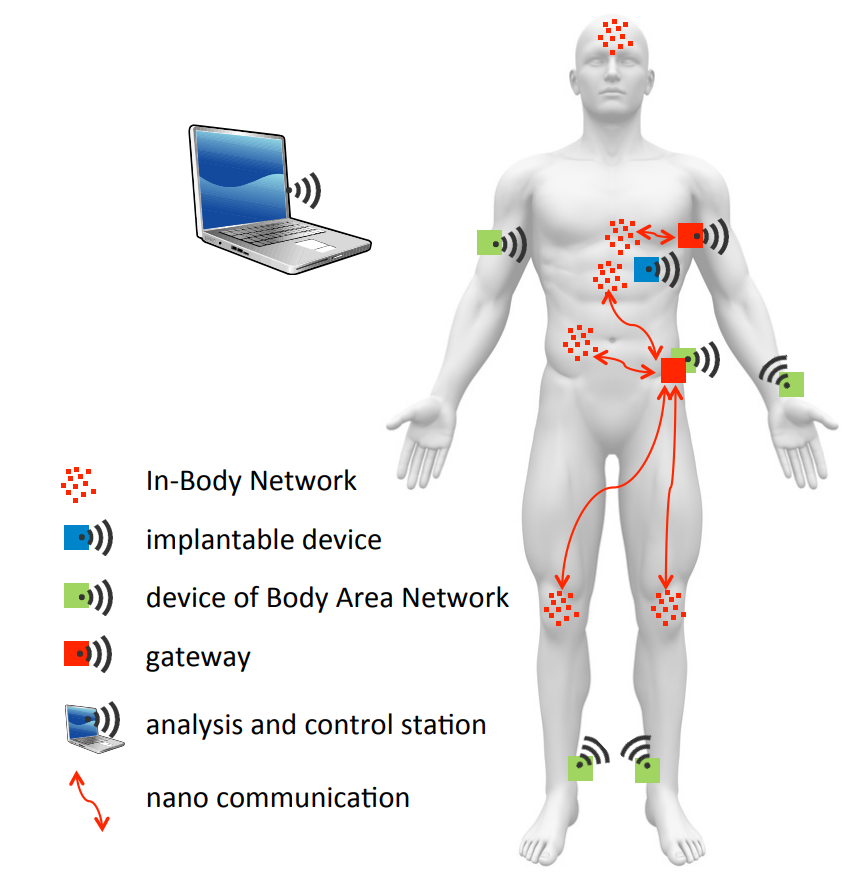
\includegraphics[width=0.53\textwidth]{images/In-Body_Networks.png}
	\caption[In-Body-Netzwerke]{In-Body-Netzwerke kombiniert mit einem Body-Area-Network (BAN). Eine Kontrollstation, welche für die Analyse von Daten zuständig ist, kommuniziert über drahtlose Verbindungen mit im Körper implantierten Geräten. Diese Geräte können wiederum miteinander oder über ein Gateway mit In-Body-Networks kommunizieren.\cite{dressler2015nanothings}}
	\label{fig:in-body_network}
\end{figure}

Wie zuvor angedeutet, gibt es einige verschiedene Anwendungsgebiete für Nanotechnologien und im Besonderen für Nanonetzwerke.
Das größte und möglicherweise wichtigste Anwendungsgebiet ist jedoch die Medizin \cite{gu2013diabetes,li2018nanorobo,wang2015light,yao2017factors}.
Nanopartikel im Spezifischen werden beispielsweise schon länger zur Krebsbekämpfung eingesetzt \cite{singhal2010cancer}.

Es lassen sich auch andere mögliche Anwendungsgebiete für diese Technologie finden, wie beispielsweise in der Geologie \cite{jin2019mapping}, in der Agrartechnik \cite{almpanis2019agent,axelos2017agri} oder in der Materialindustrie \cite{ma2010qca,taibi2019light}. Doch die Fähigkeit von Nanonetzwerken, auf einem deutlich kleineren Skalenbereich als herkömmliche Netzwerke zu agieren, verleiht ihnen ein hohes Potenzial für Anwendungen im Bereich der Humanmedizin.

Zwar werden einige diese Technologien heute schon verwendet, doch das Potenzial ist noch lange nicht voll ausgeschöpft.
So können diese bereits implementierten Technologien in ein \emph{In-Body-Network} (IBN) zusammengefügt werden.
Das theoretische Nanonetzwerk funktioniert mit einer Kontrollstation, die mit Geräten verbunden ist, die beispielsweise unter der Haut eines Menschen implantiert werden können.
Diese Geräte werden wiederum dafür verwendet, um über den menschlichen Blutkreislauf miteinander und mit der externen Kontrollstation zu kommunizieren.
Ein solches System kann nicht nur die Vitalwerte des Körpers überwachen, sondern diese Daten zur Analyse und Auswertung an die Kontrollstation geben.
Wiederum kann die Kontrollstation anhand der ausgewerteten Daten Anweisungen an das In-Body-Network senden, das daraufhin entsprechende Medikamente an spezifischen Stellen des Körpers anwenden kann.
Ein solches Netzwerk, wie es in Abbildung~\ref{fig:in-body_network} dargestellt ist, kann mit heutigem Stand zwar noch nicht \emph{in-vivo} (im lebendigen Organismus) realisiert werden, doch die theoretischen Modelle sind schon so weit, dass sie auf mathematischer Ebene funktionsfähig sind.

Jedoch gibt es bislang keine konkreten Ansätze, um die kleinschrittige Kommunikation mit DNA-Tiles und ihrer Self-Assembly zu regeln. Wie kann Information in Self-Assemblies abgebildet werden? Welche Mechanismen aus herkömmlichen Kommunikationsprotokollen lassen sich auf einer so kleinen Ebene übersetzen? Wie funktioniert Adressierung oder Fehlererkennung in einer Self-Assembly? Diese und andere Fragen haben dazu geführt, dass diese Arbeit sich kleinschrittiger und tiefer mit diesem Thema der Nanonetzwerke befasst.

\section{Der wissenschaftliche Beitrag dieser Arbeit}
Diese Arbeit soll eine umfangreiche Grundlage für die Kommunikation mit DNA-Tile-basierten Self-Assemblies schaffen. Die Ansätze und Ideen sollen dementsprechend möglichst allgemein gehalten werden, sodass sie für verschiedene Anwendungsgebiete angepasst werden können. Auch soll mit dieser Arbeit ein Gefühl übermittelt werden, welche Mechanismen herkömmlicher Kommunikationsprotokolle mit Tile-basierter Self-Assembly implementierbar sind und welche nicht. Leser*innen dieser Arbeit sollen am Ende Inspiration und Gedankenanstöße für eigene Forschung auf dem Gebiet erhalten.

\section{Struktur der Arbeit}
Die Arbeit ist in sieben Kapitel unterteilt. Nach der Einleitung in diesem Kapitel folgen mit Kapitel~\ref{cha:grundlagen} die Grundlagen für DNA-basierte Nanonetzwerke. In den Grundlagen finden sich Informationen über DNA, verschiedene Tilebildungsverfahren von DNA-Strängen, Self-Assembly der Tiles und Assemblymodelle. Auch werden Grundlagen zu herkömmlichen Kommunikationsprotokollen geliefert. Nach den Grundlagen werden in Kapitel~\ref{cha:relatedwork} wissenschaftliche Arbeiten näher betrachtet, da diese eine besondere Nähe zu dieser Arbeit besitzen.

Nach den Grundlagen werden in Kapitel~\ref{cha:konzept} die Konzepte vorgestellt, die für die Umsetzung von Mechanismen aus herkömmlichen Kommunikationsprotokollen auf Nanoebene notwendig sind. Von Adressierung, Routing, Fehlererkennung, Fehlerkorrektur, Framing, Datenflusskontrolle, Nachrichtencodierung zu Flags, werden verschiedene Ideen modelliert und vorgestellt. Einige dieser Ideen wurden in einem Python Skript \marginnote{\qrcode[height=1cm]{https://github.com/Falkenheim/Tile-Generator}} implementiert, das Tilesets für die Simulationsumgebung NetTAS verändert oder generiert. Das Skript und die Umsetzung der Mechanismen werden in Kapitel~\ref{cha:konstruktion} vorgestellt.

Die betrachteten Tilesets und ihre Simulationsergebnisse werden im Kapitel~\ref{cha:simulationen} analysiert und ausgewertet. In Kapitel~\ref{cha:zusammenfassung} wird abschließend eine Zusammenfassung der Arbeit geliefert.

Da eine Motivation und ein grober Überblick für die Arbeit geliefert wurde, kann mit dem detaillierteren Inhalt der Arbeit begonnen werden.
























%Keine Überschrift ohne Text $\dots$

%\section{Das Lübecker Holstentor}
%\label{sec:holstentor}

%\subsection{Zitieren}
%\label{sec:cite}

%Das Eigenbase-Projekt \cite{Akyildiz2008a} ist sehr cool.

%\subsection{Grafik}

%See also Grafiken in commands.tex ab Zeile 341 für subfigures etc.
%\begin{figure}[htbp]
%	\begin{center}
%		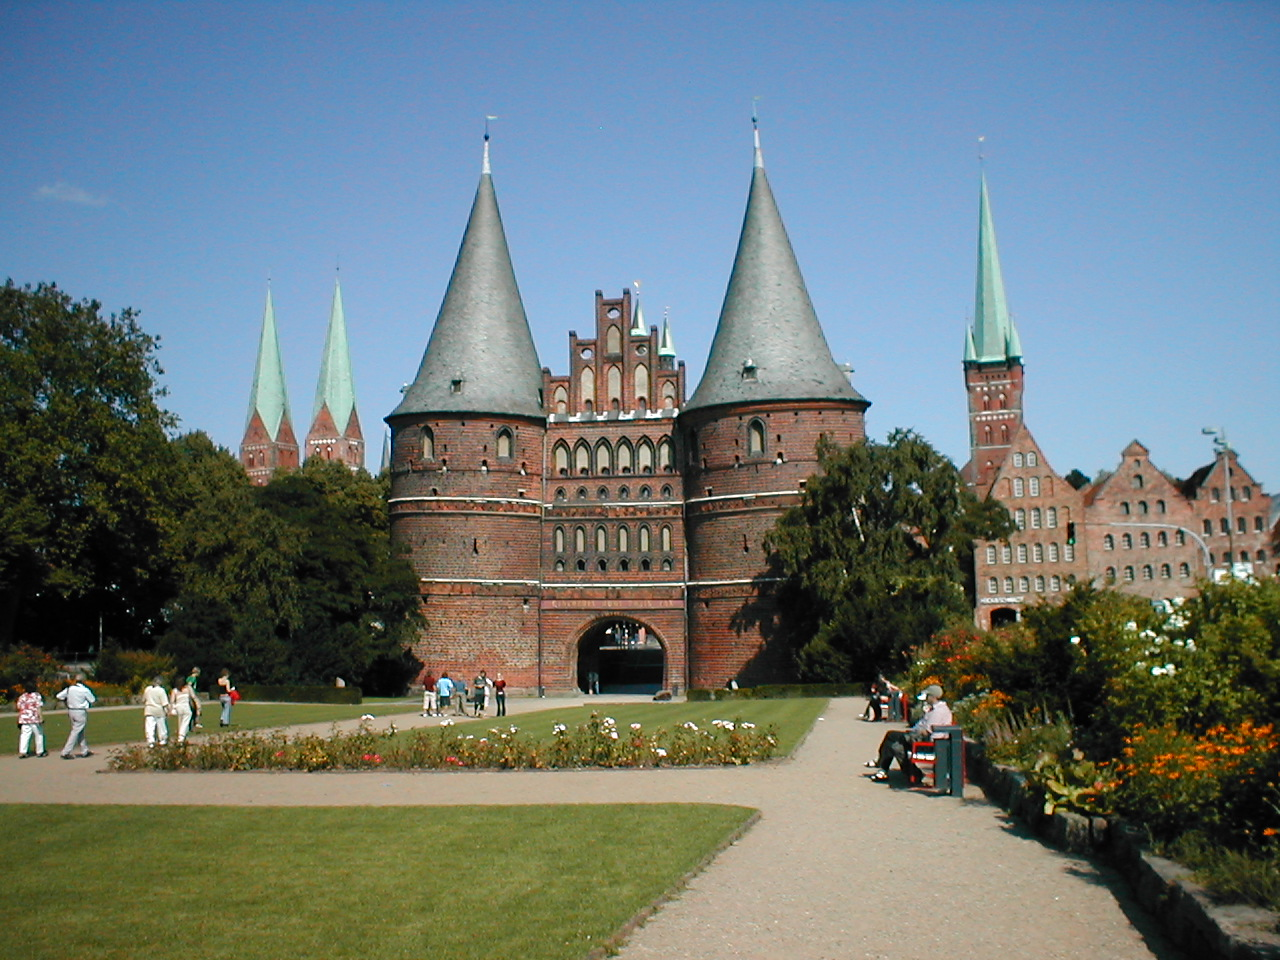
\includegraphics[width=0.75\textwidth]{images/LuebeckHolstentor}
%		\caption[Kurzfassung für Abbildungsverzeichnis]{Ausführlicher Titel}
%		\label{fig:Holstentor}
%		\end{center}
%\end{figure}

%Cref ergänzt automatisch Abbildung oder Tabellle etc.
%In \Cref{fig:Holstentor} sehen wir das \todo{Eine Randnotiz!} Lübecker Holstentor.

%\subsection{Tabelle}

%\begin{table}
%\centering
%\footnotesize
%\caption[Kurze Tabellenüberschrift]{Lange Tabellenüberschrift}
%\label{tab:eins}
%\begin{tabular}{p{1.4cm} p{2.0cm} p{2.0cm}}\toprule
%			& A 			& B 		\\[0.1cm]\midrule
%	1		& w				& s 		\\[0.2cm]
%	2 		& e				& f			\\[0.2cm]
%	3		& r				& s			\\[0.2cm]
%	4 		& t				& n 		\\\bottomrule
%\end{tabular}
%\end{table}

%In \Cref{tab:eins} sehen wir...

%\subsection{Gleichung}

%\begin{equation}\label{eq:test}
%  a=b
%\end{equation}

%In \Cref{eq:test} sehen wir...

%\subsection{Code-Listing}

%\lstinputlisting[label={lst:hello}, caption={This is a code.}]{helloworld.cpp}


%In \Cref{lst:hello} wird...

%\subsection{Zitat}

%Ein Zitat aus der Wikipedia:

%\begin{quote}
%	\begin{myquote}
%		Die Universität zu Lübeck ist eine Hochschule in der Hansestadt Lübeck (Deutschland), die 1964 zunächst als zweite Medizinische Fakultät der Universität Kiel eingerichtet wurde. Studienangebot und Forschungstätigkeit der Universität zu Lübeck haben ihren Ausgangspunkt in der Medizin.
%		\label{quote:uni}
%	\end{myquote}
%\end{quote}

%\todo[inline,color=green!40,caption={Kurzversion des Todos}]{Ein Inline-Todo}

%
% Hinweis: CRef funktioniert nicht für Zitate! Bitte \quoteref{...} verwenden
%
%In \quoteref{uni}...

%\todo[inline]{Mit Besitzer und Datum}

%\newpage

%Etwas mehr Inhalt auf einer weiteren Seite

%\newpage

%Etwas mehr Inhalt auf noch einer tollen Seite

	\chapter{Grundlagen}
\label{cha:grundlagen}

Dieses Kapitel liefert wichtige Grundlagen für die Arbeit. 
Zu Beginn werden Nanonetzwerke eingeführt und einige ihrer Herausforderungen erläutert. 
Anschließend folgt die Definition von DNA-Tile-basierten Nanonetzwerken mit der Konstruktion, Modellierung und Darstellung dieser Systeme.
Zum Abschluss des Kapitels geht es um die Kommunikationsprotokollschichten, die in dieser Arbeit besonderes Augenmerk erhalten, da sie auf die DNA-Tile-basierte Nanonetzwerkebene abstrahiert werden sollen.

\section{Einführung in Nanonetzwerke}

Der Begriff \emph{Nanonetzwerk} umfasst allgemein alle Strukturen, die Netzwerken ähneln und auf dem Skalenbereich der Nanoebene existieren. Auch wenn in dieser Arbeit nur DNA-Tile-basierte Nanonetzwerke betrachtet werden, ist es sinnvoll, zu Beginn allgemeinere Eigenschaften von Nanonetzwerken zu betrachten.

Nanonetzwerke dienen zur Kommunikation von Teilnehmern in einem Netzwerk auf Nanoebene. Auch wenn sie in ihren Aufgaben der Kommunikation zwischen Teilnehmern des Netzwerks herkömmlichen Netzwerken ähneln, gibt es bedeutende Unterschiede.
Nanonetzwerke haben eine höhere Teilnehmeranzahl als die meisten herkömmlichen Netzwerke. 
Da sie auf einem kleinen Skalenbereich funktionieren, wird dieser Faktor vorwiegend durch eine hohe Menge an Teilnehmern ausgeglichen, um für den Skalenbereich große Distanzen überbrücken zu können.
Auch weisen die meisten Nanonetzwerke eine hohe Heterogenität auf, da ein Nanogerät häufig nur eine spezifische Aufgabe übernehmen kann. Darüber hinaus existiert in den meisten Nanonetzwerken keine zentrale Kontrollinstanz, da diese auf Nanoebene schwer zu realisieren ist. So kann eine Steuerung wie im Beispiel aus Kapitel~\ref{cha:einleitung} von außen durch beispielsweise ein \emph{Body-Area-Network} (BAN) geregelt werden.\cite{buether2017formal}

Da sich Nanonetzwerke so stark von herkömmlichen Netzwerken unterscheiden, ist es schwierig, ein herkömmliches \emph{Kommunikationsprotokoll} in einem Nanonetzwerk unverändert anzuwenden.
Kommunikationsprotokolle sind in der Informatik seit vielen Jahren von zentraler Bedeutung. 
Sie definieren die Regeln und Verfahren für die Übertragung von Daten zwischen verschiedenen Endgeräten und Netzwerken. 
Ein zentraler Bestandteil der Kommunikation von verteilten Geräten ist die \emph{Synchronisation}. Für die Kommunikation von verteilten Systemen entwickelte Lamport im Jahr 1978 wichtige Grundlagen \cite{lamport1978time}. In der Informatik haben Mechanismen und Ansätze zur Synchronisation in herkömmlichen Netzwerken erhebliche Fortschritte gemacht, auch wenn sie immer noch nicht optimal sind. Auf Nanoebene ist die Synchronisation noch anspruchsvoller und muss meist über asynchrone Kommunikation oder andere Ansätze umgangen werden. Somit können einige Mechanismen zur Synchronisation eines Systems in Nanonetzwerken ausgeschlossen werden.\cite{buether2017formal}

In dieser Arbeit werden einige Kommunikationsprotokolle und -mechanismen auf die Nanoebene abstrahiert und analysiert. Bevor diese Mechanismen jedoch näher betrachtet und auf die Nanoebene übersetzt werden können, müssen im Folgenden einige Grundlagen aufgestellt werden.

\section{Grundlagen der DNA}
Die \emph{Desoxyribonukleinsäure} (DNS oder DNA) ist ein Schlüsselbaustein in der Informationsstruktur lebender Organismen, da sie den genetischen Code enthält. Da die Bezeichnung DNA gebräuchlicher ist als die deutsche Abkürzung DNS, wird im Folgenden immer von DNA die Rede sein. Dieser Code besteht aus einer Sequenz der organischen Basen Adenin (A), Guanin (G), Cytosin (C) und Thymin (T). Die spezifische Anordnung dieser Basen bildet den genetischen Code, der die Produktion von Proteinen und folglich die biologischen Funktionen von Zellen und Organismen steuert. \cite{alberts2015molecular}

Die grundlegende Struktur der DNA wurde erstmals im Jahr 1953 von Watson und Crick als Doppelhelix-Struktur vorgestellt \cite{watson1953molecular}. Diese Doppelhelix besteht aus zwei entgegengesetzten Strängen von Zucker- und Phosphat-Molekülen, die durch Basenpaare (A-T und G-C) miteinander verbunden sind, wie in Abbildung~\ref{fig:dna_doppelhelix} dargestellt. Diese Struktur ist fundamental für die Fähigkeit der DNA zur Selbsterhaltung und Replikation. Durch sie wird in lebenden Organismen das Informationsmanagement ermöglicht.

\begin{figure}
	\centering
	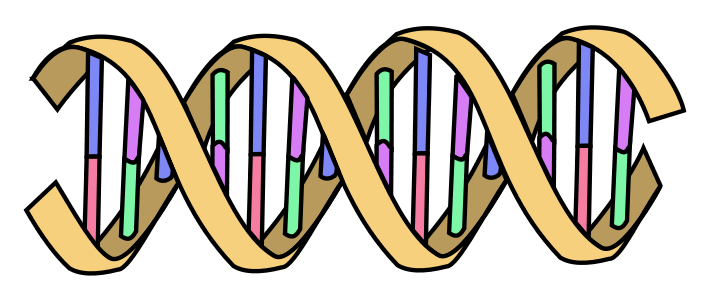
\includegraphics[width=0.8\textwidth]{images/DNA_Doppelhelix_Farbe.png}
	\caption[DNA Modell]{Ein farbcodiertes DNA Modell. Zu sehen ist das Zuckerphosphatrückgrat (gelb), das durch Basenpaare aus Adenin (A) und Thymin (T) oder Guanin (G) und Cytosin (C) verbunden ist.\cite{wikiFigDNA}}
	\label{fig:dna_doppelhelix}
\end{figure}

Das Konzept der DNA-Replikation wurde erstmals im Jahr 1958 von Meselson und Stahl beschrieben. Dabei handelt es sich um den Prozess, bei dem ein DNA-Molekül in zwei identische Kopien geteilt wird \cite{meselson1958replication}. Dieser Prozess beginnt mit der Denaturierung oder Trennung der Doppelhelix in zwei einzelne Stränge. Jeder dieser Einzelstränge dient dann als Vorlage für die Synthese eines neuen, komplementären Strangs. Dabei erkennt und bindet ein Enzym namens DNA-Polymerase die komplementären Basen (A zu T und C zu G) an den Einzelstrang. Dies führt zur Bildung einer exakten Kopie des ursprünglichen DNA-Strangs.

Diese Grundkenntnisse über die Struktur und den Replikationsmechanismus der DNA sind essenziell für das Verständnis der molekularen Genetik und können in der Nanotechnologie insbesondere bei der DNA-basierten Datenspeicherung genutzt werden. Die Fähigkeit der DNA zur Selbsterhaltung und Replikation ermöglicht die Erstellung genauer Kopien von Daten, was einen robusten und effizienten Mechanismus für die Datensicherung bietet.

\section{Self-Assembly}

\begin{figure}
	\centering 
	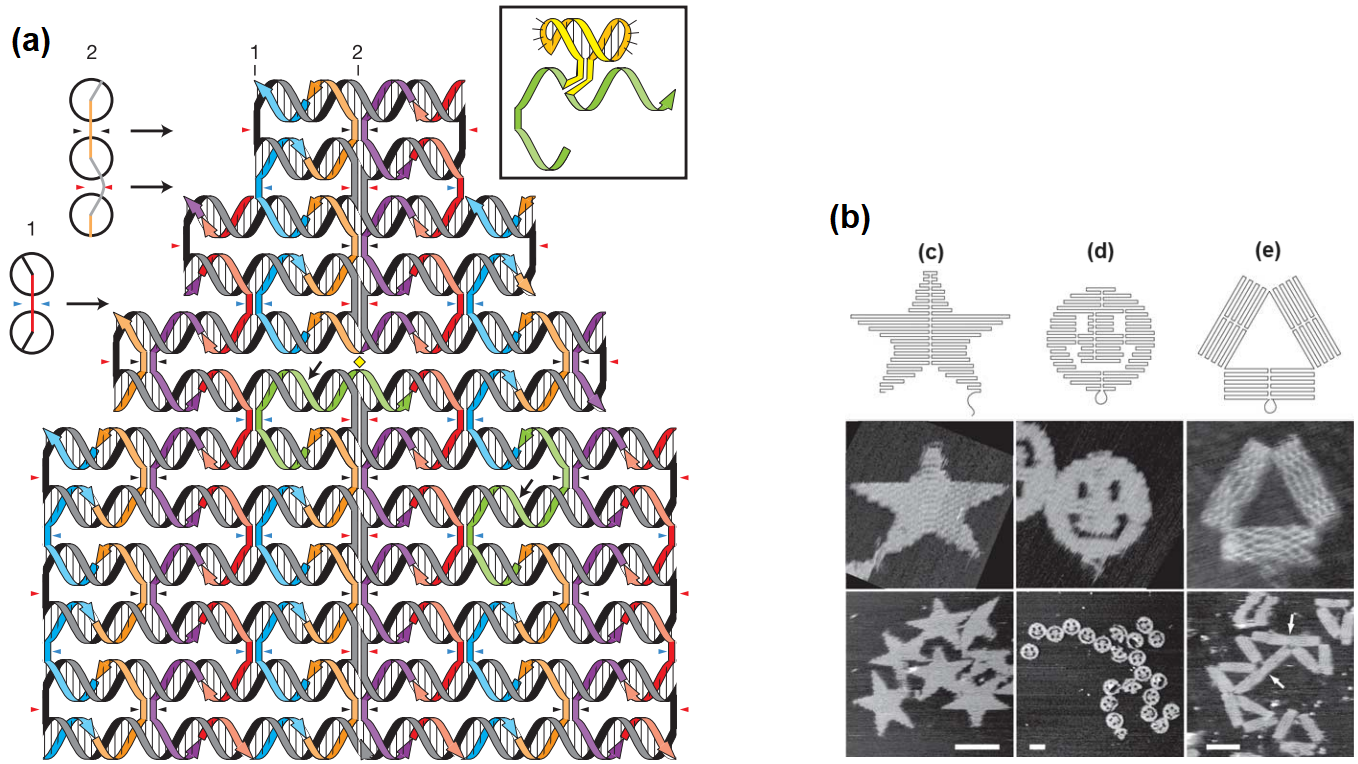
\includegraphics[width=0.9\textwidth]{DNA_Origami_Roth.png}
	\caption[DNA Origami]{DNA Origami aus der Arbeit von Rothemund \cite{rothemund2006origami}. 
	Dabei ist in (a) die Konstruktion eines langen DNA Strangs zu sehen, der durch Überkreuzungen und DNA Klammern in die gewollte Form gebracht werden kann. 
	In (b) wird ein Machbarkeitsbeweis gegeben. 
	Rothemund hat dafür verschiedene Strukturen erstellt. Von oben nach unten: Modell, Nahaufnahme einer Konstruktion und Aufnahme der Gesamtstruktur. 
	Hier abgebildet sind die folgenden Formen: ein Stern (c), ein Smiley (d) und ein Dreieck aus Rechtecken (e)}
	\label{fig:dna_origami}
\end{figure}

Für diese Arbeit von besonderem Interesse ist die \emph{DNA Self-Assembly}. 
Dabei wird DNA verwendet, um Strukturen zu bilden, die ohne weiteres äußeres Einwirken selbstständig und selbstorganisiert von den DNA-Strängen gebildet werden. Diese Technik bietet einen Bottom-Up Ansatz zur Bildung von komplexeren Strukturen auf der nanoskalaren Ebene. 

Die Grundlagen für DNA Self-Assembly legten Seeman et al. bereits in den 1980er Jahren. 
Es entstand die Idee davon, die Eigenschaften der Basenpaare gezielt zu nutzen, um die Moleküle in einer bestimmten Art und Weise anzuordnen.\cite{seeman1982dna}

Ein weiterer Grundbaustein der DNA Self-Assembly ist die Arbeit von Chad A. Mirkin et al. aus dem Jahr 1996. 
In ihrer Arbeit \glqq A DNA-based method for rationally assembling nanoparticles into macroscopic materials\grqq\, stellen die Forschenden eine Technik vor, durch die synthetisierte Goldnanopartikel durch DNA-Moleküle reversibel in spezifische Muster und Strukturen geordnet werden.\cite{mirkin1996assembling} 

Auf Basis dieser Grundbausteine wurden einige Ansätze zur DNA Self-Assembly entwickelt. 
Einer dieser Ansätze ist das \emph{DNA-Origami}. 
Erstmals vorgestellt im Jahr 2006 von Paul Rothemund, zeigte diese Technik, dass durch DNA Self-Assembly beliebige Strukturen zuverlässig konstruiert werden können. 
Ein DNA-Origami Molekül, sowie einige von Rothemund erstellte Strukturen sind in Abbildung~\ref{fig:dna_origami} zu sehen.\cite{rothemund2006origami}

%\begin{figure}
%	\centering
%	\begin{subfigure}{0.45\textwidth}
%		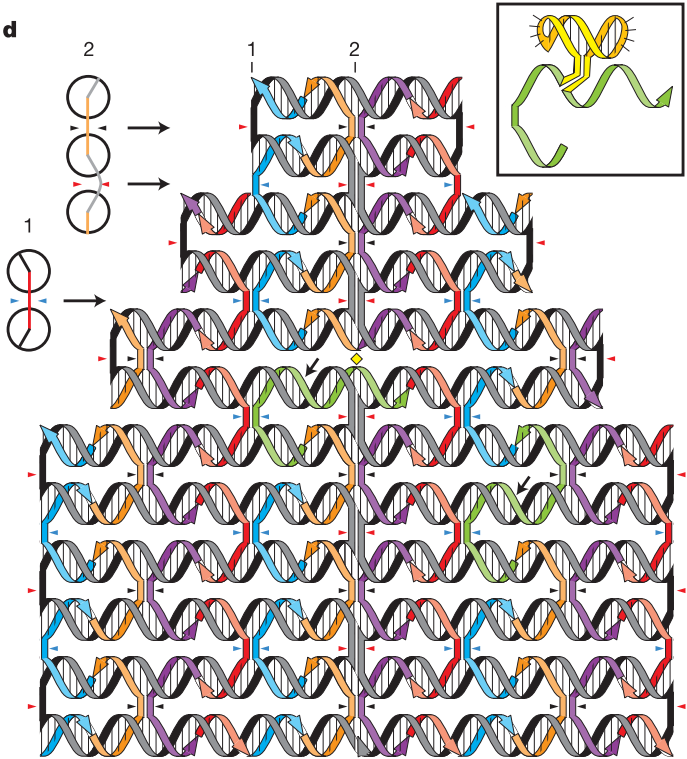
\includegraphics{DNA_Origami_Roth_A.png}
%		\subcaption{(a)}
%		\label{fig:dna_origami_a}
%	\end{subfigure}
%	\quad
%	\begin{subfigure}{0.45\textwidth}
%		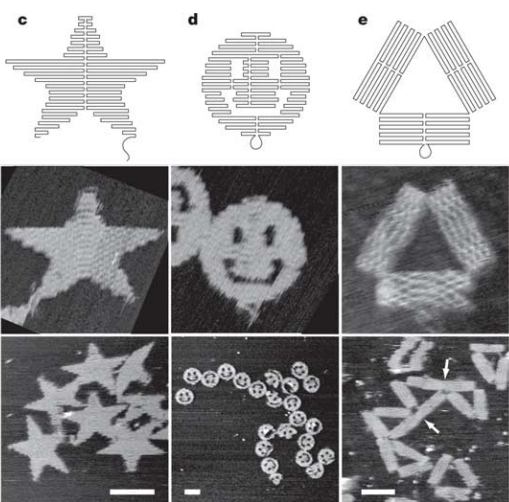
\includegraphics[width=\textwidth]{DNA_Origami_Roth_B.png}
%		\subcaption{(b)}
%		\label{fig:dna_origami_b}
%	\end{subfigure}
%	\caption{Test}
%	\label{fig:dna_origami}
%\end{figure}

Die von Rothemund vorgestellte Technik lässt sich ohne Probleme auch auf dreidimensionale Strukturen übertragen, wie die Arbeit von Ke et al. zeigt. \cite{ke2009origami3d}

\section{Tile-basierte Self-Assembly}

\begin{figure}
	\centering
	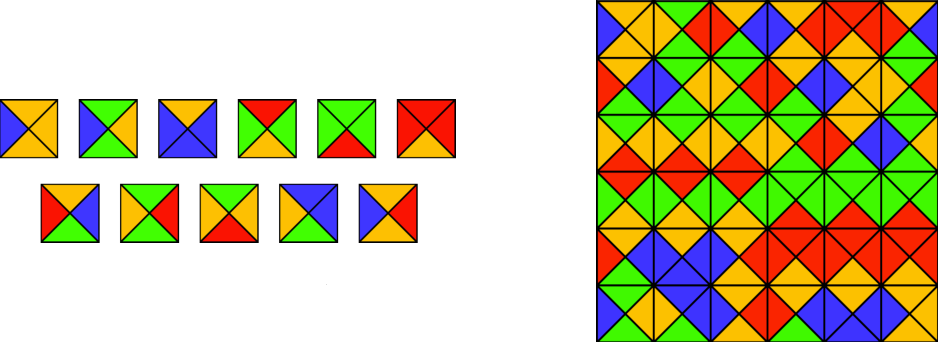
\includegraphics[width=0.65\textwidth]{images/Wang_Tiles.png}
	\caption[Wang Tiles]{Links Wang Tiles, die sich rechts zu einer lückenlosen Struktur zusammenfügen lassen.\cite{matsushima2016verfication}}
	\label{fig:wang_tiles}
\end{figure}

Basierend auf der zuvor beschriebenen Konstruktion von Nanostrukturen auf DNA-Basis, wird nun die \emph{Tile-basierte Self-Assembly} vorgestellt. 
Die theoretische Basis dieser Art der Self-Assembly sind die nach ihrem Erfinder benannten: die \emph{Wang Tiles}. 
Wang Tiles werden meist durch Quadrate mit vier farbigen Seiten dargestellt, wie in Abbildung~\ref{fig:wang_tiles} zu erkennen ist. 
Ein Tile aus einer Menge von Wang Tiles kann sich in einem $\mathbb{Z}^2$ Bereich nur mit anderen Tiles verbinden, wenn die Farben mit allen verbundenen Tiles übereinstimmen. 
Dieses Verhalten kann mit einem Puzzle verglichen werden und lässt sich direkt auf die Bindung von DNA-Tiles übertragen.\cite{wang1990tiles}

\begin{figure}
	\centering
	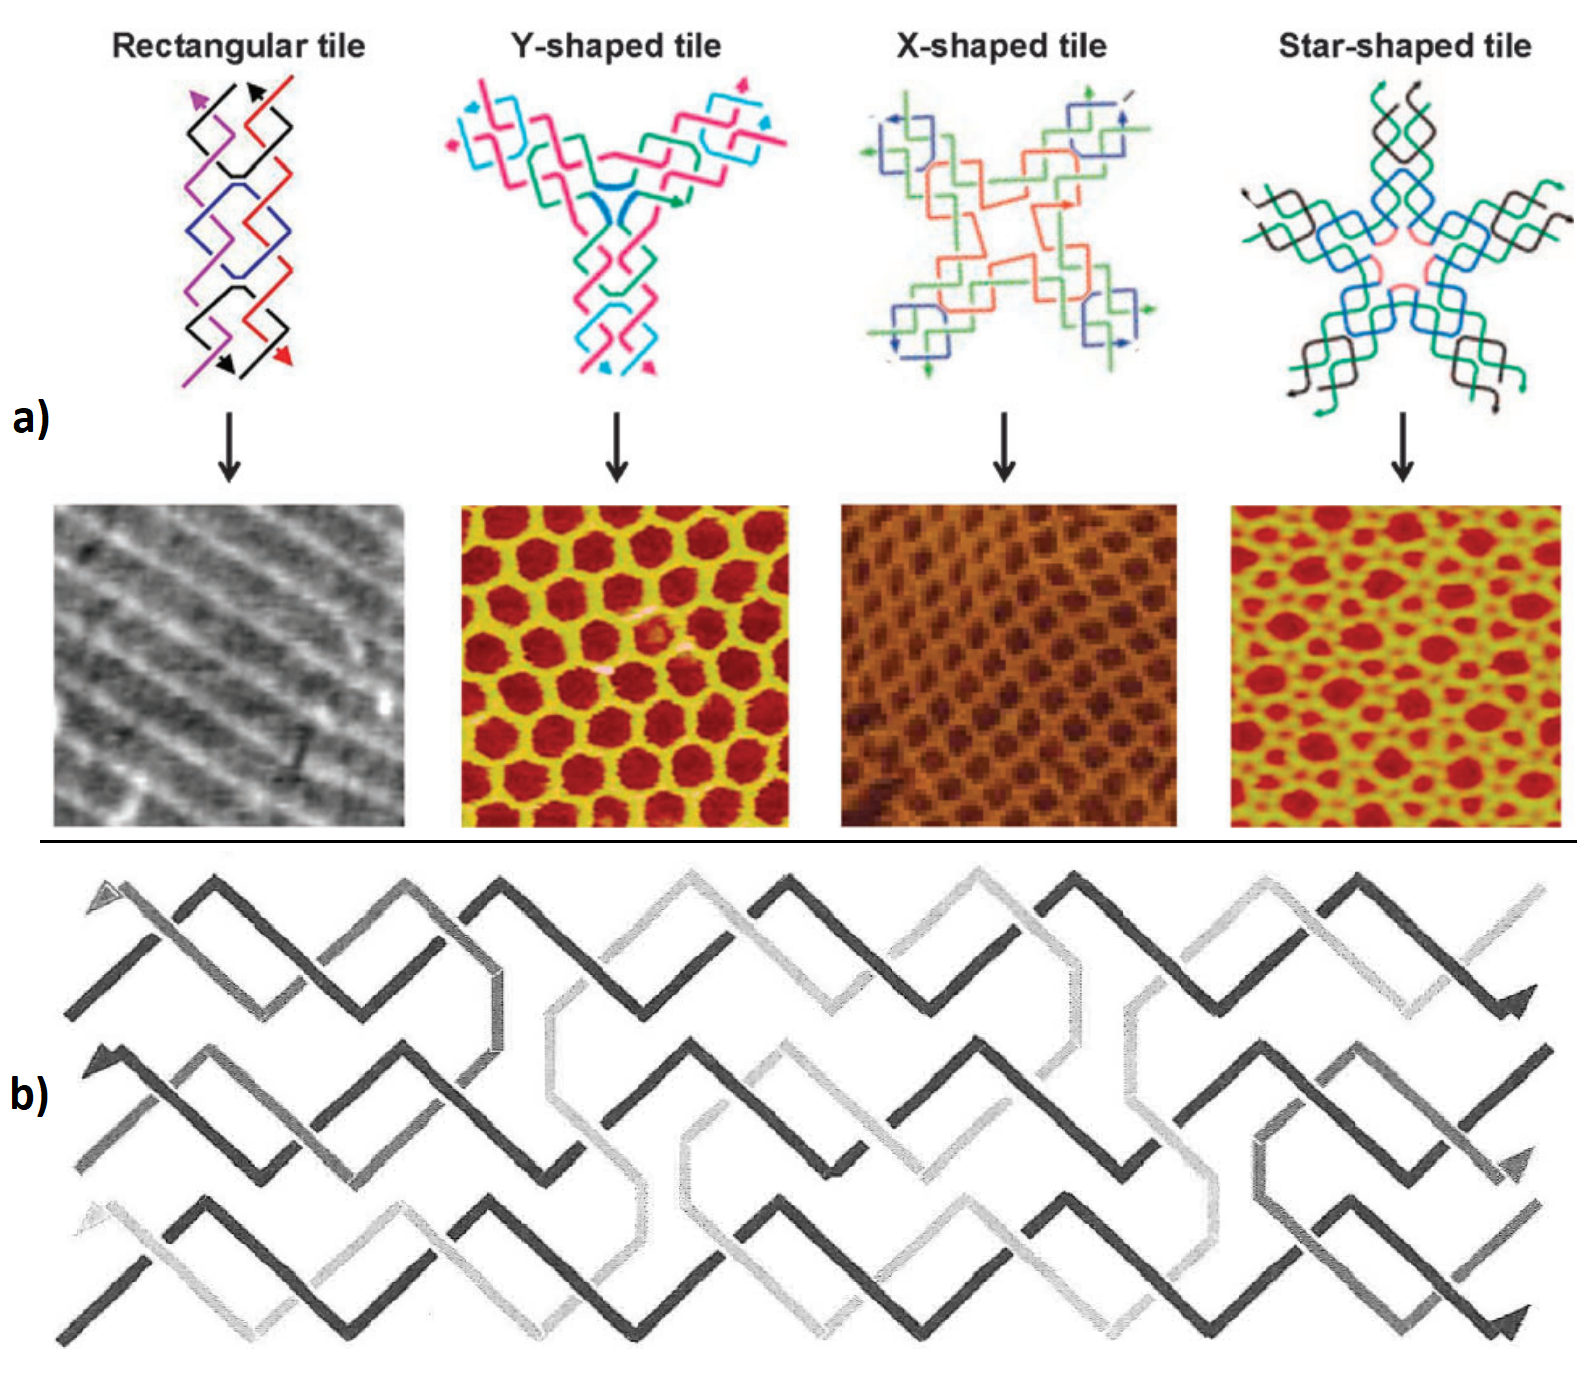
\includegraphics[width=0.8\textwidth]{images/DX_TX-Tiles.png}
	\caption[DX- und TX-Tiles]{Darstellung von zwei verschiedenen Tile-Strukturen. In a) ist das \emph{double-crossover-tile} (DX-tile) dargestellt \cite{roh2011materials}. Von links nach rechts ist eine Rechteckform, eine Y-Form, eine X-Form und eine Sternform zu sehen. Unten sind Aufnahmen der Strukturen unter einem Mikroskop dargestellt. In b) ist das Modell eines Triple-Crossover-Tiles (TX-Tiles) aus der Arbeit von Winfree et al. abgebildet \cite{winfree2000tx}. }
	\label{fig:dx_tx_tiles}
\end{figure}

Dafür werden im Weiteren einige DNA-Tiles vorgestellt. 
Es gibt verschiedene Arten von DNA-Tiles. In dieser Arbeit werden im Folgenden DX-Tiles, TX-Tiles und Holliday Junctions betrachtet. 
Diese sollten für einen allgemeinen Überblick von DNA-Tiles ausreichen, der in dieser Arbeit benötigt wird.

Die \emph{Double-Crossover-Tiles} (DX-Tiles) wurden 1993 von Fu und Seeman vorgestellt \cite{fu1993dx}. Dabei werden zwei Doppelstränge miteinander verwoben. 
Wie ganz links in Abbildung~\ref{fig:dx_tx_tiles} a) zu sehen ist, besteht die so entstandene Struktur aus zwei äußeren Strängen (orange und violett) und zwei inneren Strängen (schwarz und blau). 
Diese Verwebung von DNA bildet eine stabile Struktur. Dabei ist zu erkennen, dass das DX-Tile in dieser Grundform mehrere offene Stränge auf beiden Seiten hat. 
Es lassen sich damit weitere Strukturen wie zum Beispiel die Y-Form, X-Form oder Sternform bilden.
Auch ermöglichen die offenen Stränge die Verbindung von mehreren DX-Tiles, wodurch größere Strukturen durch Self-Assembly ermöglicht werden. Dies ist unten in Abbildung~\ref{fig:dx_tx_tiles} a) in den Aufnahmen der gebildeten Strukturen zu erkennen.

Eine Erweiterung der DX-Tiles bilden die \emph{Triple-Crossover-Tiles} (TX-Tiles). 
Vorgestellt wurden sie von Winfree et al. im Jahr 2000 \cite{winfree2000tx}. 
Durch die Verwebung von drei Doppelsträngen ist diese Struktur noch stabiler.
Außerdem ermöglicht das TX-Tile das Bilden von komplexeren Strukturen als das DX-Tile, da es einen größeren Abstand zwischen den offenen Enden aufweist.
Ein solches TX-Tile ist in Abbildung~\ref{fig:dx_tx_tiles} b) zu sehen.

Von besonderem Interesse für diese Arbeit sind die \emph{Holliday Junctions}. 
Von Seeman et al. \cite{kallenbach1983immobile} in ihrer Arbeit aus dem Jahr 1983 das erste Mal in einem Machbarkeitsbeweis vorgestellt, stammt diese Verbindung von DNA-Strängen aus der Feder von Holliday \cite{holliday1974molecular}.
Da diese Verbindung vier offene Enden in verschiedenen Richtungen hat, bietet sie sich gut zum Bilden von komplexeren Strukturen an. 
Wie in Abbildung~\ref{fig:holliday} zu erkennen ist, besteht eine Holliday Junction aus vier Strängen, die jeweils mit zwei anderen Strängen verbunden sind. 
Dabei entstehen vier offene Enden, die sich je nach Sequenz der Basenpaare nur mit ausgewählten anderen Strängen verbinden können. 
Aus Abbildung~\ref{fig:holliday} lässt sich ableiten, dass die Ausrichtung der vier offenen Enden variieren kann.
Für diese Arbeit wird jedoch nur die Ausrichtung in vier unterschiedliche Richtungen relevant sein.

Da somit der Prozess zur Bildung von DNA-Tiles vorgestellt wurde, kann im Weiteren die Modellierung und mathematische Darstellung der Tiles besprochen werden.

\begin{figure}
	\centering
	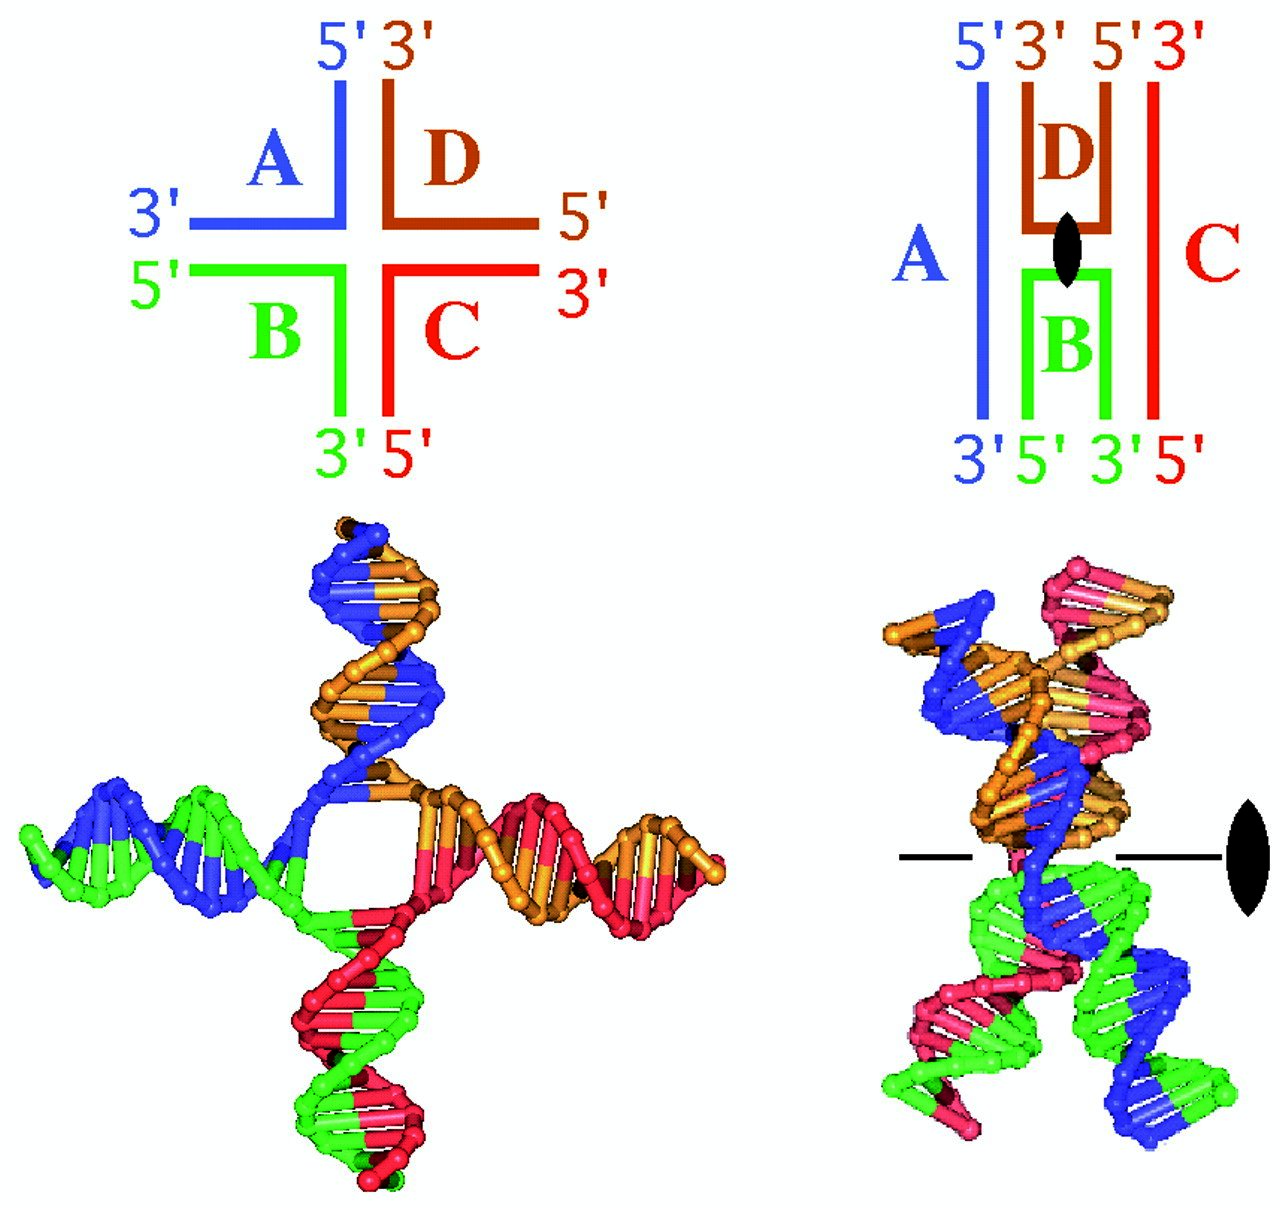
\includegraphics[width=0.5\textwidth]{images/Holliday_Junction.png}
	\caption[Holliday Junction]{Darstellung der Holliday Junction. Oben die Schemata von zwei möglichen Verbindungen. Unten die daraus entstandenen Modelle.\cite{brandt2000holliday}}
	\label{fig:holliday}
\end{figure}

\section{Nanogeräteklassen}
Um Modelle von Nanonetzwerken aus Nanogeräten und ihren Nachrichten erstellen zu können, müssen die verschiedenen Nanostrukturen zuerst definiert werden. Hierfür werden Definitionen aus der Arbeit von Büther et al. herangezogen \cite{buether2017formal}. Um Nanogeräte definieren zu können, müssen zuerst einige Kategorien festgelegt werden. 
Dazu zählen \emph{Aktuatoren} $A$, eine Komponente für die \emph{Kommunikation} mit anderen Geräten $C$, eine Komponente zur \emph{Informationsverarbeitung} $I$, eine Komponente zur \emph{Fortbewegung} $L$, ein \emph{Speicher} für Daten und Programme $M$\!, eine \emph{Energieversorgung} $P$\!, \emph{Sensoren} $S$ und \emph{Zeitgeber} $T$.

Um spezifische Nanogeräte definieren zu können, muss zu Beginn eine allgemeine Definition anhand der Kategorien zu Nanostrukturen gegeben werden. 

\begin{definition}
	Eine \emph{Nanostruktur} $\mathcal{N}_S = K_{opt}$ ist ein nanogroßes, künstliches Konstrukt, das konzipiert wurde, um eine spezifische Funktion in einer Umgebung $\Gamma$ zu erfüllen. Eine Nanostruktur besteht aus null oder mehr optionalen Komponenten $K_{opt}$. Diese sind definiert als $K_{opt} \subseteq \{A,C,I,L,M,P,S,T\}$.
\end{definition}

Eine einheitliche und klare Definition für \emph{Nanogröße} findet sich in der Literatur nicht, da sie sich je nach Angabe zwischen einem Nanometer und wenigen Mikrometern bewegt. 
Sie wird hier jedoch trotzdem verwendet, unter der Annahme, dass für den jeweiligen Anwendungsfall die Maximalgröße einer Nanostruktur beachtet wird.
Mit dieser allgemeinen Definition können im Weiteren Nanogeräte definiert werden.

\begin{definition}
	Ein \emph{Nanogerät} $\mathcal{N}_D = K_{mand} \cup K_{opt}$ ist eine Nanostruktur. Es besteht aus einer Menge notwendiger Komponenten $K_{mand} = \{P\}$ und einer Menge aus null oder mehr optionalen Komponenten $K_{opt} = \{A,C,I,L,M,S,T\}$.
\end{definition}

Um ein Nanogerät von einer passiven Nanostruktur unterscheiden zu können, benötigt das Nanogerät eine autarke Energieversorgung $P$. Die restlichen Komponenten sind wie auch bei den Nanostrukturen optional.
So können verschiedene Nanogeräte näher definiert werden.

\begin{definition}
	Eine \emph{Nanomaschine} $\mathcal{N}_M = K_{mand} \cup K_{opt}$ ist ein Nanogerät mit notwendigen Komponenten $K_{mand} = \{A,P\}$ und einer Menge aus null oder mehr optionalen Komponenten $K_{opt} \subseteq \{C,I,L,M,S,T\}$, in einer Umgebung $\Gamma$.
\end{definition}

\begin{definition}
	Ein \emph{Nanosensor} $\mathcal{N}_{Se} = K_{mand} \cup K_{opt}$ ist ein Nanogerät mit notwendigen Komponenten $K_{mand} = \{P,S\}$ und einer Menge aus null oder mehr optionalen Komponenten $K_{opt} \subseteq \{A,C,I,L,M,T\}$, in einer Umgebung $\Gamma$.
\end{definition}

\begin{definition}
	Ein \emph{Nanoknoten} $\mathcal{N}_{N} = K_{mand} \cup K_{opt}$ ist ein Nanogerät mit notwendigen Komponenten $K_{mand} = \{P,C\}$ und einer Menge aus null oder mehr optionalen Komponenten $K_{opt} \subseteq \{A,I,L,M,S,T\}$, in einer Umgebung $\Gamma$.
\end{definition}

Nanomaschinen, Nanosensoren und Nanoknoten sind in dieser Definition Nanogeräte, die entweder Aktuatoren $A$, Sensoren $S$ oder Kommunikationskomponenten $C$ besitzen. Analog zu diesen Definitionen lassen sich im Folgenden auch Nanoroboter definieren.

\begin{definition}
	Ein \emph{Nanoroboter} oder \emph{Nanobot} $\mathcal{N}_{R} = K_{mand} \cup K_{opt}$ ist ein programmierbares Nanogerät mit einem hohen Grad an Autonomie in einer Umgebung $\Gamma$. Es besteht aus einer Menge notwendiger Komponenten $K_{mand} = \{A,I,M,P,S\}$ und einer Menge aus null oder mehr optionalen Komponenten $K_{opt} \subseteq \{C,L,T\}$.
\end{definition}

Alle diese Nanostrukturen beziehungsweise Nanogeräte lassen sich mengentheoretisch mit ihren Überschneidungen in Abbildung~\ref{fig:nanostruktur} darstellen.

\begin{figure}
	\centering
	\resizebox{0.7\textwidth}{!}{
	\begin{tikzpicture}{scale=0.65}
		%% \draw[use as bounding box] (-4.2,-3.2) rectangle (4.2, 2.8);
		% \useasboundingbox (-4.2,-3.2) rectangle (4.2, 2.8);
		\fill[
		pattern=north east lines, pattern color=blue!30!white]
		(0,-1.6) ellipse[x radius=3, y radius=1.2];
		\fill[
		pattern=vertical lines, pattern color=lightgray]
		(-1.1,0) ellipse[x radius=3, y radius=1.7];
		\fill[
		pattern=horizontal lines, pattern color=green]
		(1.1,0) ellipse[x radius=3, y radius=1.7];
		\fill[
		pattern=crosshatch dots, pattern color=black!40!white]
		(0, 0) ellipse[x radius=1.7, y radius=1];
		\fill[
		pattern=crosshatch dots, pattern color=green]
		(-3.6,2.3) ellipse[x radius=1.35, y radius=1.1];
	
		\draw (-3.6,2.3) ellipse[x radius=1.35, y radius=1.1];
		\draw (0,-0.2) ellipse[x radius=6, y radius=5];
		\draw (0,-0.2) ellipse[x radius=5.2, y radius=4];
		\draw (0,-0.2) ellipse[x radius=4.2, y radius=3];
		\draw (0,-1.6) ellipse[x radius=3, y radius=1.2];
		\draw (-1.1,0) ellipse[x radius=3, y radius=1.7];
		\draw (1.1,0) ellipse[x radius=3, y radius=1.7];
		\draw (0,0) ellipse[x radius=1.7, y radius=1];
	
		\node[align=center] at (-3.55,2.35) (A2) { \contour{white}{Moleküle}\\\contour{white}{Cluster}\\\contour{white}{Fullerene} \\\contour{white}{Nanopartikel} };
		\node at (0,4.2) (A1) {Nanoobjekt $\mathcal{N}_{O}$};
		\node at (0,3.2) (A0) {Nanostruktur $\mathcal{N}_{S}$};
		\node at (0,2.2) (A) {Nanogerät $\mathcal{N}_D$};
		\node[align=center] at (-3,0) (B) { \contour{white}{Nano-}\\ \contour{white}{sensor $\mathcal{N}_{So}$}};
		\node[align=center] at (3,0) (C) { \contour{white}{Nano-}\\ \contour{white}{maschine $\mathcal{N}_M$}};
		\node at (0,0.1) (D) {\contour{white}{Nanoroboter $\mathcal{N}_R$}};
		\node at (0,-2.2) (E) {\contour{white}{Nanoknoten $\mathcal{N}_N$}};
	\end{tikzpicture}}
	\caption[Nanostrukturen Venn-Diagramm]{Venn-Diagramm verschiedener Nanostrukturen und ihren Überschneidungen.\cite{lau2020phd}}
	\label{fig:nanostruktur}
	\end{figure} 

\section{Tile-Assembly Modelle}
Neben der Definition von Nanostrukturen müssen für diese Arbeit eindeutig definierte Modelle und Modellierungverfahren vorgestellt werden, um Nanonetzwerke modellieren zu können.
Dafür werden in den folgenden Absätzen das \emph{Abstract Tile-Assembly Model} (aTAM), das \emph{Kinetic Tile-Assembly Model} (kTAM), das \emph{Two-Handed Tile-Assembly Model} (2HAM) und das \emph{Kinetic Two-Handed Tile-Assembly Model} (kTHAM) definiert. Um diese Modelle vorstellen zu können, müssen jedoch zu Beginn einige grundlegenden Begriffe definiert werden. Alle folgenden Notationen und Definitionen basieren auf den Arbeiten von Lutz et al. \cite{lathrop2009strict} und Patitz \cite{patitz2014introduction}.

\begin{definition}
	Ein $n$-dimensionales \emph{Tile} $t_n$ ist ein Objekt in $\mathbb{Z}^n$ mit Einheitslänge und 90 Grad Winkeln. 
	Eine \emph{Seite} eines Tiles $t_n$ ist durch einen Vektor $u_i \in U_t \subseteq \mathbb{Z}^n$ definiert. $U_t$ ist eine Menge von eindeutigen Richtungsvektoren. 
	Der Gegenvektor $-u_i$ beschreibt die gegenüberliegende Seite von $u_i$ in derselben Dimension. Der Vektor $u_i$ hat genau einen Eintrag, der ungleich $0$ ist. Die Seiten eines Tiles sind durch folgende Relation definiert:
	\begin{align*}
		\text{Seite: }t_n \mapsto \underbrace{U_t\times U_t\times \dots\times U_t}_n
	\end{align*} 
\end{definition}

In dieser Arbeit werden hauptsächlich zweidimensionale Tiles von Bedeutung sein. Daher wird im Folgenden immer von zweidimensionalen Tiles gesprochen, wenn die Dimension nicht angegeben ist.

In jedem \emph{Tile Assembly System (TAS)} gibt es eindeutig definierte Regeln, durch die sich zwei Tiles miteinander verbinden können. Dafür wird Folgendes definiert:

\begin{definition}
	Ein \emph{Kleber} oder \emph{Glue} $g\in G$, wobei $G$ die Menge der möglichen Kleber beschreibt, ist durch einen \emph{Bezeichner} oder ein \emph{Label} $\mathcal{L}_g\in\Sigma^*$ definiert, wobei $\Sigma$ ein Alphabet ist und $s\in\mathbb{N}$ eine \emph{Kleberstärke} mit den Funktionen:
	\begin{align*}
		\text{label : }& G\mapsto\Sigma^* \\
		\text{strength : }& G\mapsto\mathbb{N}
	\end{align*}
\end{definition}
\begin{definition}
	Zwei Tiles $t$ und $t'$, die durch $v_t$ und $v_{t'}\in\mathbb{Z}^n$ definierte Orte belegen, sind genau dann benachbart, wenn $|v_t-v_{t'}| = 1$ und der resultierende Vektor $e = v_t-v_{t'}$ genau ein Element ungleich $0$ hat.
\end{definition}
Ein Tile kann auf allen Seiten immer nur genau einen oder keinen Nachbarn haben.
\begin{definition}
	Die \emph{Temperatur} $\tau$ eines TAS beschreibt die minimale Stärke des Klebers $s$ für eine stabile Verbindung.
\end{definition}
Damit ein Tile in einem TAS eine stabile Verbindung aufbauen kann, muss die absolute Kleberstärke des Tiles mindestens der Temperatur des Systems entsprechen. Die absolute Kleberstärke ergibt sich aus der Summe aller Kleberstärken des Tiles mit den verbundenen anderen Tiles.
\begin{definition}
	Ein \emph{$n$-dimensionaler Tiletyp} $T_n$ ist eine Schablone für ein Tile $t_n$. Ein $n$ dimensionaler Tiletyp wird durch einen Bezeichner $\mathcal{L}_T\in\Sigma^*$ und einer Menge von Klebern $g_i\in G$ definiert. Ein Kleber befindet sich an jeder Seite $u_{t,i}\in U_t$ von $t_n$. Folgende Funktionen sind jedem Tiletyp zugeordnet:
	\begin{align*}
		\text{glue : }& T_n\times U_t\mapsto G \\
		\text{strength : }& g\in G \mapsto \mathbb{N}
	\end{align*}
\end{definition} 
Eine so definierte Tileschablone kann wie in Abbildung~\ref{fig:dna_tile_math} dargestellt werden. 
Hierbei bekommt jedes Tile eine eindeutige Beschriftung, in diesem Beispiel ist es die \glqq 1\grqq.
Auf den vier Seiten des Tile kann so mit einer weiteren Beschriftung die \emph{Farbe}, der \emph{Kleberbezeichner}, dargestellt werden.
Der Kleberbezeichner wird durch die Sequenz der Basenpaare an den offenen Enden definiert. Dies ist in Abbildung~\ref{fig:dna_tile_bio} zu erkennen. 
Nur wenn der Kleberbezeichner von zwei Tiles gleich ist, können sich die Tiles im Zuge der Self-Assembly verbinden. 
Im Beispiel aus Abbildung~\ref{fig:dna_tile_math} sind die Kleberbezeichner mit den Beschriftungen \glqq A,B,C,D\grqq\, gegeben. 
Außerdem wird die Kleberstärke des Tiles durch ausgefüllte schwarze Boxen an den Seiten des Tiles dargestellt. 
Dabei entscheidet die Menge an schwarzen Boxen die Stärke des Klebers.

Die Verbindung zweier Tiles funktioniert wie folgt:
\begin{definition}
	Zwei Tiles $t$ und $t'$ \emph{binden korrekt} bei Temperatur $\tau$, wenn folgende Bedingungen gelten:
	\begin{align*}
		&(1)~ t \text{ und } t' \text{ sind benachbart.}\\
		&(2)~ \exists u_i\in U_t: label(glue(t,u_i)) = label(glue(t',-u_i)) \\
		&\qquad\qquad\quad~~\land strength(glue(t,u_i)) \geq \tau \land strength(glue(t',-u_i)) \geq \tau
	\end{align*}
	Wenn eine der beiden Bedingungen $(1)$ oder $(2)$ verletzt wird, wird diese Verbindung \emph{Error} oder \emph{false} genannt.
\end{definition} 

\begin{figure}
	\centering
	\begin{tikzpicture}[scale=2.0]
		\tileBsp{1}{1}
	\end{tikzpicture}
	\caption[Mathematisches Schema eines DNA-Tiles]{Mathematisches Schema eines DNA-Tiles. Die schwarzen Boxen stellen dabei die Stärke des Klebers auf den jeweiligen Seiten dar (hier 1). Die Beschriftungen (A, B, C, D) stellen die Farbe oder die Kleberbezeichner dar. Mit der \glqq 1\grqq\, wird das Tile beschriftet und gibt damit dem Tile einen Namen, um Beschreibungen und Analysen einfacher zu machen.}
	\label{fig:dna_tile_math}
\end{figure}


\begin{figure}
	\centering
	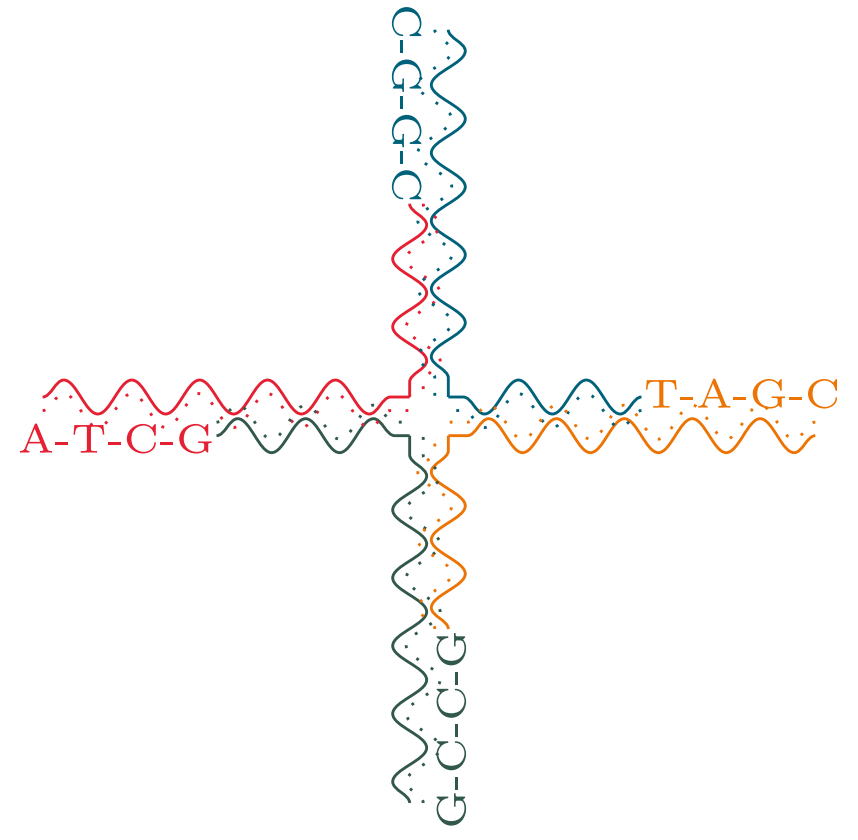
\includegraphics[width=0.5\textwidth]{images/DNA_Tile.png}
	\caption[Biologisches Schema einer Holliday Junction]{Biologisches Schema einer Holliday Junction, deren vier offenen Enden so gewählt wurden, dass sie sich oben und unten sowie rechts und links mit sich selbst verbinden kann.\cite{lau2019dnatiles}}
	\label{fig:dna_tile_bio}
\end{figure}
Die Verbindung von mehreren Tiles wird \emph{Assembly} genannt.

\begin{definition}
	Eine n-dimensionale \emph{Tile Assembly} oder \emph{Assembly} ist eine partielle Funktion $\alpha:\mathbb{Z}^n\mapsto T$ mit $T$ als Menge von n-dimensionalen Tiles. Eine Assembly $\alpha$ ist \emph{$\tau$-stabil}, wenn kein Tile $t_n\in T$ aus der Assembly entfernt werden kann, ohne dafür Kleber der Stärke $\tau\in\mathbb{N}$ entfernen zu müssen. 
\end{definition}

\begin{definition}
	Die \emph{Grenze} einer Assembly $\alpha$ ist eine Teilmenge von $\alpha$. Diese Menge enthält alle Tiles mit mindestens einem freien Nachbar-Tile.
\end{definition}

\begin{definition}
	Die \emph{Wachstumsfront} einer $n$-dimensionalen Assembly $\alpha$ ist eine Teilmenge von $\mathbb{Z}^n$. Eine Stelle ist nur dann Teil der Wachstumsfront, wenn folgende Bedingungen eintreffen:
	\begin{align*}
		&(1) \text{ Die Stelle ist nicht belegt.}\\
		&(2) \text{ Die Stelle liegt an der Grenze der Assembly.}\\
		&(3) \text{ Die benachbarte Seite des Tiles an der Grenze hat eine minimale Kleberstärke } 1.
	\end{align*}
\end{definition}

In einer gegebenen Assembly ändern sich sowohl die Grenzlinie als auch die Wachstumsfront kontinuierlich durch die Prozesse des Hinzufügens und Entfernens von Tiles. Wenn eine Assembly zu einem Zeitpunkt keine offenen Enden mit einer Kleberstärke von größer oder gleich eins aufweist, dann existiert für diese Assembly keine Wachstumsfront. Trotz dieser dynamischen Veränderungen verfügt jede Assembly zu jedem Zeitpunkt über eine klar definierte Grenze.

Das erste Tile einer Assembly, bezeichnet als $\alpha_0$ zum initialen Zeitpunkt $t=0$, erhält die Bezeichnungen \emph{Seed-Assembly} oder \emph{Seed-Tile} und wird als $\sigma$ gekennzeichnet. An der Wachstumsfront dieser Seed-Assembly kann die Anbindung weiterer Tiles auf einer nichtdeterministischen Basis erfolgen.

Im Folgenden werden die Modelle definiert, die in Kapitel~\ref{cha:simulationen} zur Simulation und Evaluation der Ergebnisse verwendet werden.

\begin{definition}
	Ein \emph{Tile Assembly Model (TAM)} ist ein Tupel $\mathcal{T}_\tau = (T,\sigma,\tau)$, mit $T$ als endliche Menge von Tiles (auch \emph{Tileset} genannt), $\sigma$ der Seed-Assembly und $\tau\in\mathbb{N}$ als Temperatur des TAM. 
\end{definition}

\begin{definition}
	$\mathcal{A}[\mathcal{T}]$ ist die Menge aller terminierten Assemblies, die als Ergebnis eines TAM in endlicher Zeit erreicht werden können. 
	Eine Assembly $\alpha\in\mathcal{A}[\mathcal{T}]$ gilt als \emph{terminiert $(\alpha_{\square})$}, wenn kein weiteres $\tau$-stabiles Tile in der Assembly hinzugefügt werden kann.
\end{definition}

\begin{definition}
	Sei $\alpha_i$ eine durch ein TAM definierte Assembly. Eine \emph{Assembly Sequenz} ist eine Sequenz $S=<\alpha_0,\alpha_1,\dots>$, wobei $\alpha_{i+1}$ die Assembly $\alpha_i$ mit einem weiteren hinzugefügten Tile darstellt. 
	Wenn die Sequenz $s$ endlich ist, dann wird das letzte Element der Sequenz \emph{Ergebnis $\alpha_\square$} oder \emph{terminiert} genannt.
\end{definition}

Aus diesen Definitionen kann so das erste Modell, das \emph{Abstract Tile Assembly Model (aTAM)} definiert werden:

\begin{definition}
	Sei $T$ eine Menge von Tiles, die nicht rotiert werden können. Sei $\sigma$ eine Seed-Assembly. Dann ist das Tupel $\mathcal{A} =(T,\sigma,\tau)$ ein Abstract Tile Assembly Model (aTAM) mit Temperatur $\tau$\!. In einem aTAM kann immer nur ein einzelnes Tile zu einem Zeitpunkt hinzugefügt werden. Des Weiteren können Tiles nicht wieder aus der Assembly entfernt werden.
\end{definition}

Das aTAM ist das einfachste in dieser Arbeit betrachtete Modell der Tile-basierten Assembly. 
Als Beispiel für solch eine Assembly dient Abbildung~\ref{fig:assembly_bsp}. 
Zu sehen ist ein aTAM $\mathcal{A} = (T,S,\tau)$ mit der Menge der Tiles $T=\{ \sigma,a,b,c\}$ und der Temperatur $\tau = 2$. 
Das Tileset ist links in der Abbildung dargestellt. Die Assembly Sequenz $S = <\alpha_0,\alpha_1,\alpha_2,\alpha_3>$ ist rechts zu erkennen. Da das Beispiel mit im aTAM durchgeführt wird, ist $\alpha_3=\alpha_\square$, da bei einer Temperatur von zwei keine weiteren Tiles mit dem Bezeichner \glqq C\grqq\, an der Wachstumsfront hinzugefügt werden können. Diese Verbindungen wären nicht $\tau$-stabil.

\begin{figure}
	\centering 
	\begin{tikzpicture}[scale=1.1]
		\tileAssemblyC{1}{2.5}
		\tileAssemblySigma{1}{1}
		\tileAssemblyA{2.5}{2.5}
		\tileAssemblyB{2.5}{1}
		%%%
		\node[scale = 1.2] at (4.5,3) {$\alpha_0$};
		\tileAssemblySigma{4.5}{1}
		%%%
		\node[scale = 1.2] at (6.5,3) {$\alpha_1$};
		\node[scale = 1.2] at (5.5,1.6) {$\rightarrow$};
		\tileAssemblyA{6.5}{2.2}
		\tileAssemblySigma{6.5}{1}
		%%%
		\node[scale = 1.2] at (9.1,3) {$\alpha_2$};
		\node[scale = 1.2] at (7.5,1.6) {$\rightarrow$};
		\tileAssemblyA{9.7}{2.2}
		\tileAssemblySigma{9.7}{1}
		\tileAssemblyB{8.5}{1}
		%%%
		\node[scale = 1.2] at (12.3,3) {$\alpha_3$};
		\node[scale = 1.2] at (10.7,1.6) {$\rightarrow$};
		\tileAssemblyA{12.9}{2.2}
		\tileAssemblySigma{12.9}{1}
		\tileAssemblyB{11.7}{1}
		\tileAssemblyC{11.7}{2.2}
	\end{tikzpicture}
	\caption[Beispiel Assembly]{Beispiel Assembly von vier Tiles (links) in Sequenz bei Temperatur $\tau = 2$. Im ersten Schritt $\alpha_0$ liegt nur die Seed-Assembly vor. In Schritten $\alpha_1$ und $\alpha_2$ binden sich nichtdeterministisch die Tiles \glqq A\grqq\, und \glqq B\grqq\, an der Seed-Assembly an. In Schritt $\alpha_3$ bindet sich so das Tile \glqq C\grqq. Da bei Temperatur zwei keine stabile Verbindung von zwei \glqq C\grqq-Tiles möglich ist, ist $\alpha_3$ das Resultat der Assembly.\cite{lau2019dnatiles}}
	\label{fig:assembly_bsp}
\end{figure}

Durch die Annahme, dass sich keine Tiles wieder aus der Assembly entfernen können und Schritt für Schritt immer nur ein Tile hinzugefügt werden kann, werden einige Grenzfälle in aTAM nicht betrachtet. Im Beispiel aus Abbildung~\ref{fig:assembly_bsp} könnte zum Beispiel durch Hinzufügen von drei \glqq C\grqq\, Tiles, wieder eine stabile Verbindung gebildet werden. Diese Betrachtung gibt es in aTAM jedoch nicht.
Dadurch gilt dieses Modellierungsverfahren als simpel, aber nicht realitätsnah.
Ein Modellierungsverfahren, das näher an der Realität und näher am Verhalten von DNA im Vorgang der Self-Assembly liegt, ist das \emph{Kinetic Tile-Assembly Model (kTAM)}.
Durch diese Eigenschaft wird kTAM die größte Rolle bei der Simulation und Auswertung von Kommunikationsprotokollen in dieser Arbeit spielen.
Im Gegensatz zu aTAM können sich in kTAM verbundene Tiles von der Assembly lösen. 
Außerdem ist es möglich, dass ein Tile sich an einer falschen Stelle bindet. 
Dies ist in aTAM nicht möglich. 
Um die Verbindung und Trennung von Tiles in kTAM darstellen zu können, muss jedoch erst einmal die \emph{Forward Rate} und \emph{Backward Rate} definiert werden. 

\begin{definition}
	Sei $\mathcal{T}_\tau$ ein TAM, $\sigma$ ein nicht leere Seed-Assembly und $T$ eine Menge an Tiles. Die \emph{Forward Rate} $r_f$, mit welcher Tiles $t$ in der Assembly hinzugefügt werden, wird wie folgt definiert:
	\begin{align*}
		r_f(t) = k_fe^{-G_{mc}}.
	\end{align*}
	$k_f$ beschreibt hier das Timing des Systems, $G_{mc}$ die benötigte Energie, um ein Tile zu binden \emph{(Binding Cost)}. Dabei gilt $G_{mc} > 0$.
\end{definition}
\begin{definition}
	Analog zur Forward Rate ist die \emph{Backward Rate} wie folgt definiert:
	\begin{align*}
		r_{r,b}(t) = k_fe^{-G_{se}}.
	\end{align*}
	Sie beschreibt mit welcher Rate sich Verbindungen in einer Assembly wieder lösen. $G_{se}$ beschreibt hierbei die benötigte Energie zum Lösen der Verbindung \emph{(Bond Breaking Cost)}. Durch $b$ wird die Anzahl der Verbindungen des Tiles angegeben.
\end{definition}

Daraus lässt sich im Weiteren das kTAM definieren:
\begin{definition}
	Sei $\sigma$ eine nicht leere Seed-Assembly, $T$ eine Tileset, $r_{r,b}$ die Backward Rate und $r_f$ Forward Rate. Dann ist ein Kinetic Tile Assembly Model wie folgt definiert:
	\begin{align*}
		\mathcal{K} = (T,\sigma,r_{r,b},r_f)
	\end{align*}
\end{definition}
Im kTAM leitet sich die Temperatur aus dem Verhältnis zwischen $G_{mc}$ (Binding Cost) und $G_{se}$ (Bond Breaking Cost) ab. Da die Temperatur selbst nicht explizit spezifiziert wird, wird sie implizit durch die zuvor definierten Forward und Backward Rates repräsentiert.
In kTAM wird in jedem Schritt ein nicht deterministisch ausgewähltes Tile an einer nicht deterministisch festgelegten Stelle der Assembly hinzugefügt. Eine korrekte Positionierung ist dabei um den Faktor $e^{G_{se}}$ wahrscheinlicher als eine falsche Positionierung. Außerdem ist bei falscher Positionierung die Wahrscheinlichkeit größer, dass durch die Backward Rate diese Verbindung wieder aufgelöst wird.

Ein weiteres realitätsnäheres Modell ist das \emph{Two-Handed Tile-Assembly Model (2HAM)}. 
Im 2HAM gibt es keine Seed-Assembly. Solange die Temperaturbeschränkungen eingehalten werden, kann jedes Tile und jede Assembly in allen Schritten mit anderen Assemblies interagieren. Dadurch wird eine Art Potenzmenge aller möglichen Assemblies gebildet.
Das Entfernen einer einzelnen Seed-Assembly, sowie das Verhalten beim Erzeugen einer Assembly macht dieses Modellierungsverfahren realitätsnäher.
Für die formale Definition des 2HAM müssen zunächst einige Definitionen gegeben werden:

\begin{definition}
	Zwei Assemblies $\alpha$ und $\beta$ sind disjunkt, wenn für alle Stellen in $\alpha$ und $\beta$ gilt: $\alpha\cap\beta = \emptyset$. Eine Assembly besteht immer aus mindestens einem Tile.
\end{definition}

\begin{definition}
	Der Zustand $S$ eines Tilesets $T$ ist eine Multimenge von Assemblies, für die Folgendes gilt:
	\begin{enumerate}
		\item Alle Assemblies $\alpha\in S$ sind $\tau$-stabil. Es müssen $\tau$ Kleber entfernt werden, damit sich die Assembly auflöst. 
		\item Alle Assemblies $\alpha\in S$ können aus der Menge $T$ durch korrekte Vereinigung gebildet werden.
	\end{enumerate}
\end{definition}

Der Zustand $S$ von $T$ ist als Multimenge definiert, da eine Verbindung eines Tiles mit sich selbst möglich sein muss. 
So müssen einige Elemente mehrfach in der Menge vorkommen. 
Zwei Asssemblies $\alpha$ und $\beta$ bilden eine \emph{korrekte Verbindung}, wenn ihre Verbindung $\tau$-stabil ist und $\alpha$ und $\beta$ disjunkt sind.

\begin{definition}
	Ein \emph{Two-Handed Tile Assembly Model (2HAM)} ist wie folgt definiert: Ein 2HAM ist ein Tupel $\mathcal{H} = (T,S_0,\tau)$ mit dem Tileset $T$, dem Startzustand $S_0$ und der Temperatur $\tau$.
\end{definition}
\begin{definition}
	Sei $\mathcal{H} = (T,S_0,\tau)$ ein 2HAM. Die Assembly Sequenz eines 2HAM ist eine Sequenz von Zuständen $S=<S_0,\dots,S_k>$ mit $k=\{1,\dots,\infty\}$. $S_{i+1}$ wird aus $S_i$ gebildet, indem alle möglichen Vereinigungen auf Assemblies $s,s'\in S_i$ durchgeführt werden.
\end{definition}
\begin{definition}
	Sei $\mathcal{H} = (T,S_0,\tau)$ ein 2HAM. Ein Zustand $S_i$ ist terminierend, wenn $S_{i+1}$ nach allen möglichen Vereinigungen äquivalent zu $S_i$ bleibt.
\end{definition}

Alle Definitionen zu aTAM, kTAM und 2HAM bis hier stammen aus der Arbeit von Patitz \cite{patitz2014introduction} und der Arbeit von Lathrop et al.\cite{lathrop2009strict}. Alle jetzt folgenden Definitionen zum \emph{Kinetic Two-Handed Tile-Assembly Model (kTHAM)} stammen aus der Arbeit von Kaussow in Zusammenarbeit mit Lau \cite{kaussow2022thesis}.

"Das Kinetic Two-Handed Tile-Assembly Model kombiniert die realitätsnahen Merkmale von 2HAM und kTAM. Analog zum 2HAM gibt es keine Seed-Assembly. Gleichzeitig, ähnlich wie im kTAM, können sich Verbindungen und Vereinigungen bilden, die nicht $\tau$-stabil sind, und bereits gebildete Verbindungen können in späteren Schritten wieder aufgelöst werden.

Dafür müssen wieder einige Definitionen aufgestellt werden.

\begin{definition}
	Eine \emph{korrekte Vereinigung} von zwei Assemblies $\alpha$ und $\beta$ im kTHAM ist eine Vereinigung, in der $\alpha$ und $\beta$ disjunkt sind.
\end{definition}

\begin{definition}
	Ein Zustand $S=\{A_S,C_S\}$ eines Tilesets $T$ ist ein Tupel von Multimengen von Assemblies und ein Vektor für ihre Nummer im kTHAM. Für das Tupel gilt Folgendes:
	\begin{enumerate}
		\item Alle Assemblies $A_S$ können aus $T$ durch korrekte Vereinigungen gebildet werden.
		\item Alle Assemblies $A_S$ sind einzigartig und ihre Häufigkeit des Auftretens ist durch den Vektor $C_S$ definiert.
		\item Die Zahl der Einträge in $C_S$ ist gleich der Anzahl von Assemblies in $A_S$.
	\end{enumerate}
\end{definition}

Die Forward Rate und Backward Rate sind analog zum kTAM.

\begin{definition}
	Ein \emph{Kinetic Tow-Handed Tile-Assembly Model (kTHAM)} ist ein Tupel $\mathcal{K_H} = (T,S_0,r_f,r_{r,b})$ mit der Menge an Tiles $T$, dem Startzustand $S_0$, der Forward Rate $r_f$ und der Backward Rate $r_{r,b}$.
\end{definition}
\begin{definition}
	Eine Assembly Sequenz in kTHAM ist eine Sequenz $S$ von Zuständen $S=<S_0,\dots,S_k>$ mit $k\in\{1,\dots,\infty\}$. Ein Zustand $S_{i+1}$ entsteht aus dem Zustand $S_i$ durch Trennung oder korrekten Vereinigung von zwei Assemblies. Assemblies, die nur aus einem Tile bestehen, dürfen nicht weiter getrennt werden.
\end{definition}

Das kTHAM ist durch diese Eigenschaften ein noch realitätsnäheres, jedoch rechenaufwendiges Modell. Dadurch, dass sowohl ganze Assemblies gebunden als auch wieder gelöst werden können, werden in kTHAM mehr Extremfälle betrachtet als in kTAM oder 2HAM.

Zur Behandlung von Extremfällen wird im Folgenden das Error-Handling betrachtet.

\section{Error-Handling in Tile-basierten Self-Assembly Systemen}
\label{sec:proofreading}
In dieser Sektion sollen mögliche Probleme und Fehler im Prozess der Tile-basierten Self-Assembly betrachtet werden.
Dafür ist anzumerken, dass die mathematische Darstellung und Berechnung von Self-Assemblies einige Aspekte der Realität auslässt, um die Berechenbarkeit zu garantieren. 
So kann es im mathematischen Modell wie in Abbildung~\ref{fig:dna_tile_math} nicht dazu kommen, dass das Tile rotiert. In diesem Betrachtungshorizont sind die Tiles einer Assembly immer fest ausgerichtet. 
Dies ist in der Natur nicht gegeben. 
Für realitätsnähere Betrachtungen müsste jedes Mal berechnet werden, in welcher Ausrichtung sich das Tile befindet. 
Außerdem müsste für die Evaluation der Ergebnisse beachtet werden, in welchem Kontext diese Assembly sich in der Realität zusammensetzen würde. Äußere Einflüsse könnten den Vorgang der Self-Assembly verändern. 

In Self-Assembly Systemen können jedoch auch ohne diese weiteren Betrachtungen einige \emph{Errors} entstehen, die im Folgenden vorgestellt werden sollen. Die Definitionen der Errors stammen alle aus der Arbeit von Lau et al. \cite{lau2019dnatiles}.

Es gibt drei typischerweise auftretende Errors in Self-Assembly Systemen. 
Nicht alle dieser Errors treten in jedem Modellierungsverfahren wie kTAM oder 2HAM gleichermaßen auf.
\begin{definition}
	Ein \emph{Growth-Error} entsteht, wenn ein Tile sich in der Assembly an einer Stelle verbindet, an der mindestens einer seiner Kleber eine nicht korrekte Bindung mit einem benachbarten Kleber eingeht.
\end{definition}
\begin{definition}
	Ein \emph{Facet-Error} entsteht, wenn ein Tile sich zwar an einer korrekten Stelle mit korrekten Verbindungen zwischen Klebern verbindet, die Temperaturbeschränkungen jedoch nicht eingehalten wurden.
\end{definition}
\begin{definition}
	Ein \emph{Nucleation-Error} entsteht, wenn eine Assembly mit keinem oder einem anderen Tile als der Seed-Assembly startet.
\end{definition}

In Tabelle ~\ref{tab:errors} ist dargestellt, welche Errors von den vier zuvor definierten Modellierungsverfahren berücksichtigt werden.

\begin{table}
	\centering
	\begin{tabular}{lcccc}
		\hline\textbf{Error} & \textbf{aTAM} & \textbf{kTAM} & \textbf{2HAM} & \textbf{kTHAM} \\\hline
		Growth-Error & \checkmark & \checkmark & \checkmark & \checkmark\\
		Facet-Error & $\times$ & \checkmark & \checkmark & \checkmark\\
		Nucleation-Error & $\times$ & $\times$ & \checkmark & \checkmark\\\hline
	\end{tabular}
	\caption[Self-Assembly Errors]{Tabellarische Darstellung der vier Modellierungsverfahren von DNA-Tile-basierter Self-Assembly mit den drei typischen Errors. \checkmark steht hierbei dafür, dass das TAM diesen Error modelliert, $\times$ nicht.}
	\label{tab:errors}
\end{table}

Um eine Assembly nicht so anfällig für Growth- und Facet-Errors zu machen, kann ein Verfahren namens \emph{$k\times k$-Proofreading} verwendet werden \cite{winfree2004kxk,chen2005kxk}.
Bei diesem Verfahren werden die Tiles aus der Menge der Tiles $T$ und einer Assembly $\alpha$ ausgetauscht. 
Dabei wird jedes einzelne Tile mit einem Block von $k \times k$ mit $k\in\mathbb{Z} \land k > 1$ Tiles ersetzt. 
Ein Beispiel für ein $2 \times 2$-Proofreading ist in Abbildung~\ref{fig:error_korrektur} (a) zu sehen. 
Dabei wird das obere Tile mit den vier Tiles darunter ausgetauscht. Bei der Ersetzung muss darauf geachtet werden, dass die logische Funktion des einzelnen Tiles erhalten bleibt. 
Durch $k \times k$-Proofreading wird ein Growth- oder Facet-Error nicht unmöglich. Es wird nur die Wahrscheinlichkeit reduziert, da mehrere Errors hintereinander passieren müssen.

Eine Erweiterung des $k \times k$-Proofreading ist das \emph  {Snaked-Proofreading} \cite{chen2005kxk}.
Dabei wird die innere Struktur des Blocks, der jedes Tile ersetzen soll, verändert.
Der Ansatz des $k\times k$-Proofreading bleibt jedoch erhalten. 
Durch das Entfernen eines inneren Klebers im Inneren des Blocks werden Facet-Errors bei ersten Verbindungsversuchen eines neuen Blocks erheblich reduziert. 
Dafür muss die Kleberstärke der restlichen inneren Kleber möglicherweise angepasst werden.
Dies ist in Abbildung~\ref{fig:error_korrektur} (b) zu erkennen. 
Beim Snaked-Proofreading muss der Block in einer festen Reihenfolge gebildet werden.

\begin{figure}
	\centering
	\begin{tikzpicture}[scale = 1.3]
		\tileProofkxkLU{1}{1}
		\tileProofkxkLO{1}{2.5}
		\tileProofkxkRU{2.5}{1}
		\tileProofkxkRO{2.5}{2.5}
		\node at (1.75,0) {(a)};
		\node[scale = 2.5] at (1.75,3.5) {$\Downarrow$};
		\tileProofStart{1.75}{4.75}
		%%%
		\tileProofSnakedLU{5}{1}
		\tileProofSnakedLO{5}{2.5}
		\tileProofSnakedRU{6.5}{1}
		\tileProofSnakedRO{6.5}{2.5}
		\node at (5.75,0) {(b)};
		\node[scale = 2.5] at (5.75,3.5) {$\Downarrow$};
		\tileProofStart{5.75}{4.75}
	\end{tikzpicture}
	\caption[Tile Ersetzung durch Proofreading Beispiel]{Darstellung einer beispielhaften Tile-Ersetzung zur Implementierung präventiver Errorkorrektur. Dabei zeigt (a) das $k \times k$-Proofreading und (b) das Snaked-Proofreading.\cite{lau2019dnatiles}}
	\label{fig:error_korrektur}
\end{figure}

\section{DNA-basierte Nanonetzwerke}
Da alle Grundlagen für DNA-Tile-basierten Self-Assembly vorgestellt wurden, kann die folgende Definition aus \cite{lau2020phd} betrachtet werden:
\begin{definition}
	Sei $\mathcal{T} = (T,\sigma,\tau)$ ein Tile Assembly System, wobei $T$ eine endliche Menge an Tiles ist, $\sigma$ eine Seed-Assembly und $\tau\in\mathbb{N}^+$ die Temperatur des TAS. 
	Ein \emph{DNA-basiertes Nanonetzwerk} $\mathcal{N}_\Phi$ ist ein Nanonetzwerk. Die Komponenten sind durch die Menge $\mathcal{N}_\Phi = \mathcal{N}_{Se} \cup \mathcal{N}_R \cup \mathcal{M}_\Phi$ gegeben, wobei $\mathcal{N}_{Se}$ eine Menge von DNA-basierten Nanosensoren und $\mathcal{N}_R$ eine Menge von DNA-basierten Nanorobotern ist. $\mathcal{M}_\Phi$ ist ein Tileset für eine Menge von Nachrichtenmolekülen.
\end{definition}

\begin{figure}
	\centering
	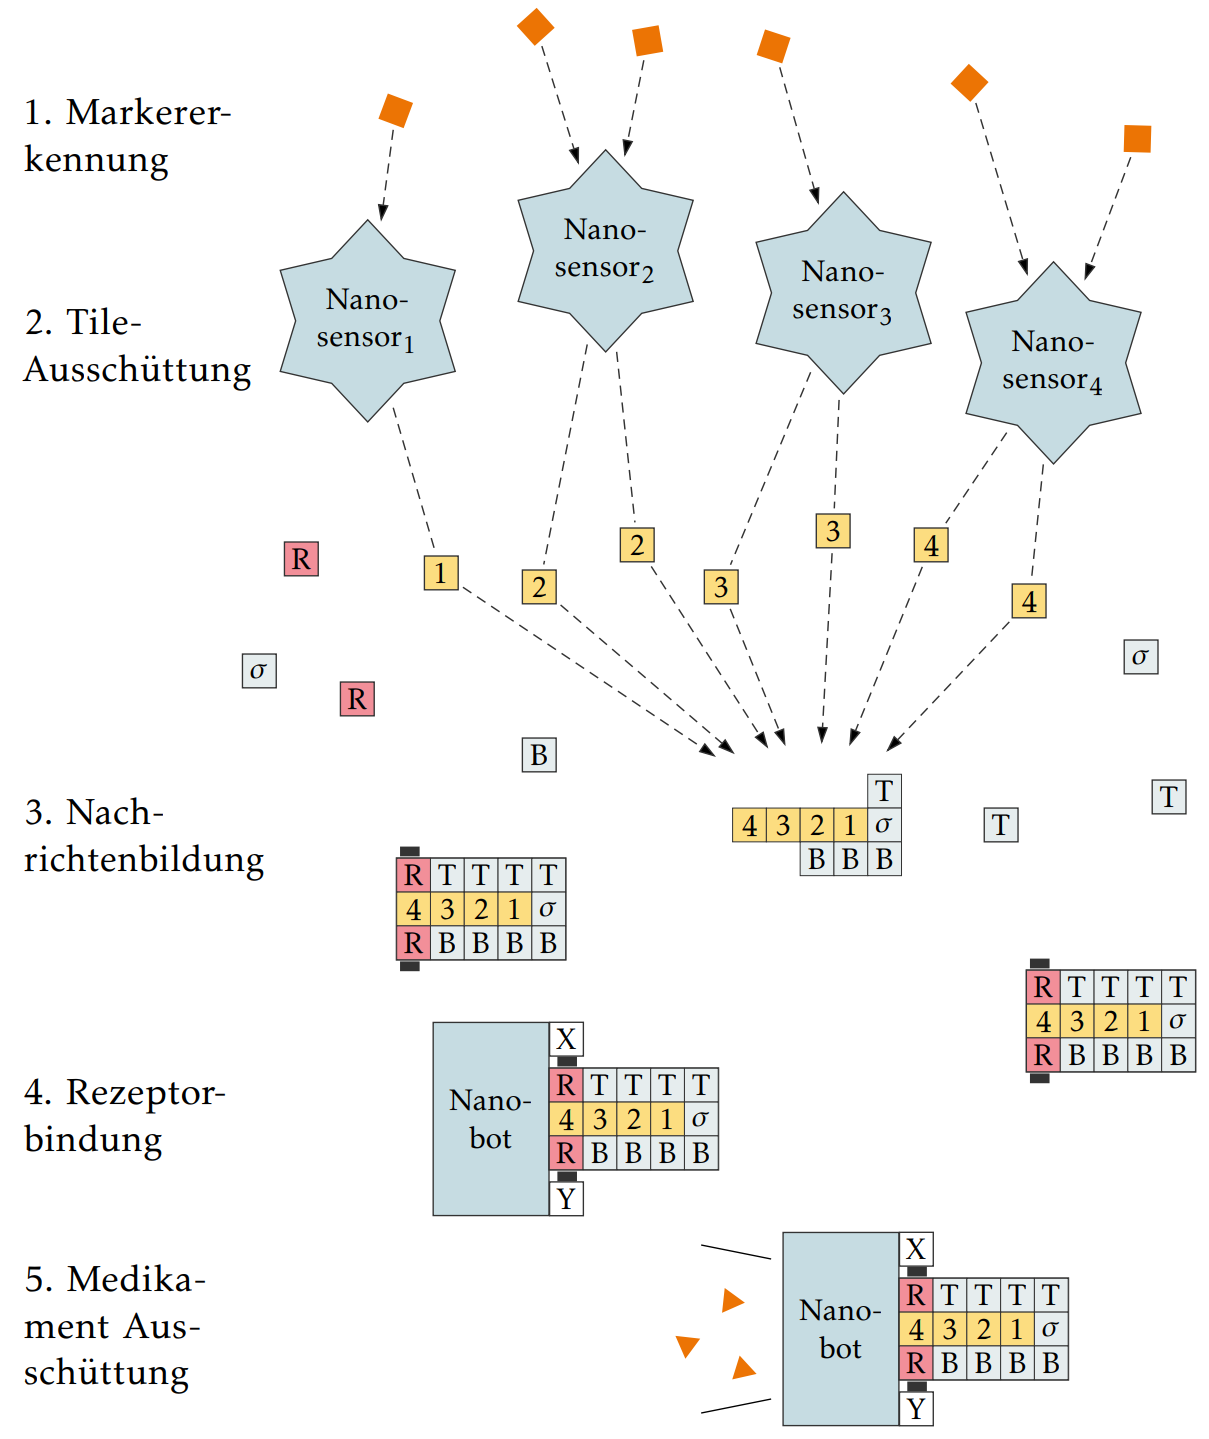
\includegraphics[width=0.9\textwidth]{images/Nanonetzwerk.png}
	\caption[Nanonetzwerk Ablauf Beispiel]{Ein beispielhafter Ablauf eines Nanonetzwerks, das ein Medikament erst dann ausschüttet, wenn vier verschiedene Sensoren Marker registriert haben. 
	Im ersten Schritt müssen Marker (hier orange) von den Nanosensoren erkannt werden, damit das System aktiviert wird. 
	Darauf folgt der zweite Schritt, in dem die Tiles ausgeschüttet werden, die zur Nachrichtenbildung benötigt werden. 
	Im dritten Schritt ist die Nachrichtenbildung dargestellt, die nur dann vollständig ist, wenn Tiles von allen vier Sensoren vorhanden sind. 
	Im vierten Schritt binden sich die Liganden der Nachricht an die Rezeptoren eines Nanoroboters. 
	Im fünften Schritt schüttet der Nanoroboter Medikamente aus, da er durch die Nachricht aktiviert wurde. \cite{lau2020phd}}
	\label{fig:nanonetzwerk_ablauf}
\end{figure}

Bei dieser Definition von DNA-basierten Nanonetzwerken ist zu beachten, dass die Nanosensoren $\mathcal{N}_{Se}$ und die Nanoroboter $\mathcal{N}_R$ korrekt aus dem Tileset $T$ gebildet werden können. 
Das muss aber nicht der Fall sein. 
In einigen Fällen kann es sinnvoller sein, die Sensoren und Roboter durch zum Beispiel DNA-Origami zu konstruieren. 
Diese Technik basiert nicht auf Tiles, sondern wie oben beschrieben auf langen DNA-Einzelsträngen und DNA-Klammern. 
Zusätzlich reduziert die eigenständige Konstruktion von Nanosensoren und Nanorobotern, beispielsweise mithilfe von DNA-Origami, die Komplexität des Tilesets $T$. 
Dementsprechend wird in dieser Arbeit der Fokus auf der Nachrichtenbildung und den dafür benötigten Tilesets liegen. 
Soweit nicht konkret von der Konstruktion von Nanosensoren oder Nanorobotern die Rede ist, wird im Folgenden bei jedem Tileset $T$ für ein Nanonetzwerk $\mathcal{N}_\Phi$ immer davon ausgegangen, dass sowohl die Nanosensoren $\mathcal{N}_{Se}$ als auch die Nanoroboter $\mathcal{N}_R$ konstruiert wurden und somit nicht im Tileset $T$ betrachtet werden müssen.

Zur Terminologie muss gesagt werden, dass hier allgemein von \emph{DNA-basierten Nanonetzwerken} gesprochen wird. Die Arbeit fokussiert sich jedoch auf die \emph{DNA-Tile-basierten Nanonetzwerke}. Das bedeutet, dass beispielsweise keine konkreten Umsetzungen von DNA-Origami-basierten Mechanismen und Geräten geliefert werden. Manchmal ist es notwendig anzunehmen, dass ein solches Gerät existiert, jedoch soll der Fokus auf den DNA-Tiles liegen.

Des Weiteren werden noch zwei neue Bausteine für die Konstruktion und Auswertung eines Nachrichtenmoleküls in einem Nanonetzwerk benötigt: \emph{Rezeptoren} und \emph{Liganden}.
Rezeptoren sind Teile eines Nanoroboters, die in der Lage sind, eine Verbindung mit Liganden einzugehen.
Liganden sind spezielle Tiles, die sich nicht nur mit einem Nachrichtenmolekül, sondern auch mit Rezeptoren eines Nanoroboters verbinden können.

Ist das Nanonetzwerk konstruiert, läuft die Kommunikation in einem solchen Netzwerk allgemein wie folgt ab:
\begin{enumerate}
	\item \emph{Markererkennung}: Die Nanosensoren des Systems können durch spezifische Marker aktiviert werden. 
	Die Art der Marker hängt von der Konstruktionsweise der Nanosensoren ab.
	Beispielsweise kann ein Nanosensor auch aus DNA-Origami gebildet werden. Durch eine Würfelform können im Inneren des Würfeln Tiles gespeichert werden. Bindet sich der Marker in Form eines DNA-Strangs, kann sich der Würfel auf einer Würfelseite öffnen.\cite{douglas2012logic}
	\item \emph{Tile-Ausschüttung}: Hat ein Nanosensor einen Marker erkannt, so schüttet dieser die Tiles aus, die zur Kommunikation im Netzwerk verwendet werden. 
	\item \emph{Nachrichtenbildung}: Die von den Sensoren freigesetzten Tiles verbinden sich durch Self-Assembly mit der bereits vorhandenen Seed-Assembly und den Liganden, um ein stabiles Nachrichtenmolekül zu bilden.
	\item \emph{Rezeptorbildung}:  Wenn die Nachricht komplett konstruiert wurde und die Liganden sich am Rand des Nachrichtenmoleküls verbunden haben, kann sich das Nachrichtenmolekül mit diesen Liganden an den Rezeptoren eines Nanoroboters binden.
	\item \emph{Nanoroboteraktivierung}: Wenn sich die Nachricht an den Rezeptoren des Nanoroboters gebunden haben, wird dieser aktiviert und erledigt die Aufgabe, für die der Nanoroboter konstruiert wurde.
\end{enumerate}

Ein Beispiel für solch eine Kommunikation ist in Abbildung~\ref{fig:nanonetzwerk_ablauf} gegeben. Hier soll ein Medikament ausgeschüttet werden, wenn vier verschiedene Sensoren ihre Marker erkennen. Dafür wird eine \glqq AND\grqq-Nachricht gebildet. 
Das Nachrichtenmolekül bildet sich nur komplett und bindet die Liganden, wenn die Tiles von allen vier Sensoren vorhanden sind. 
Diese von den Nanosensoren ausgeschütteten Tiles sind in diesem Beispiel mit \glqq 1\grqq, \glqq 2\grqq, \glqq 3\grqq\, und \glqq 4\grqq\, beschrieben.
Die Liganden sind rot mit dem Buchstaben \glqq R\grqq\, dargestellt, die Seed-Assembly durch das dafür typische $\sigma$.
Ist das Nachrichtenmolekül vollständig konstruiert, so kann es sich an den Rezeptoren (hier mit $X$ und $Y$ dargestellt) eines Nanoroboter binden.
Ist diese Verbindung fertig, wird der Nanoroboter aktiviert und lässt Medikamente aus, die dieser im Inneren gespeichert hatte.\cite{lau2020phd}

\section{Kommunikation in Nanonetzwerken}

Mit allen bis hier definierten Informationen können Nanonetzwerke erneut in Betrachtung gezogen werden. Diese Sektion wird sich auf die Kommunikation in Nanonetzwerken konzentrieren.

Die meisten Kommunikationsmethoden auf Nanoebene basieren auf \emph{Diffusion}. Dies bezeichnet die zufällige und passive Verteilung von Partikeln in einem Medium. Zu den typischen Kommunikationsmethoden, die auf diesem Prinzip aufbauen, gehören das Messen der Partikelanzahl und die Bestimmung von Konzentrationen bestimmter Partikel.
Dabei wird ein spezifischer Schwellenwert für die Partikelanzahl oder die Konzentration festgelegt, ab dem ein Ereignis als erreicht gilt. 
Wenn der Messwert den Schwellenwert überschreitet, kann dies darauf hinweisen, dass das Ereignis eingetreten ist. Es gibt jedoch Verfahren, die mehr Informationen übertragen können, aber dafür komplexere Partikelstrukturen und Messverfahren erfordern, wie das Messen von Partikeltypen und Partikelanordnungen. In solchen Fällen wird jeder Partikeltyp oder Partikelanordnung einer spezifischen Information zugeordnet. Sobald ein solcher Partikeltyp oder eine solche Anordnung durch Messungen erkannt wird, kann die entsprechende Information extrahiert werden.

In dieser Arbeit sind Tiles jedoch weiterhin die relevanteste Kommunikationsmethode. Tiles übertragen weniger Information in einem Molekül im Vergleich zum Erfassen von Partikeltypen oder -anordnungen. Allerdings ist die Bioinvasivität von Tiles deutlich geringer als bei Verfahren, die regelmäßige Messungen erfordern.\cite{farsad2016survey}

\begin{table}
	\centering
	\begin{tabular}{lll}
		\hline Problem & Signatur & Beschreibung \\\hline
		ADD & $\mathbb{Z} \times \mathbb{Z} \rightarrow \mathbb{Z}$ & Integer-Addition \\
		EQ &  $\mathbb{Z} \times \mathbb{Z} \rightarrow \{0,1\}$ & Integer-Vergleich \\
		GEQ &  $\mathbb{Z} \times \mathbb{Z} \rightarrow \{0,1\}$ & Integer-Vergleich $\geq$ \\
		LEQ &  $\mathbb{Z} \times \mathbb{Z} \rightarrow \{0,1\}$ & Integer-Vergleich $\leq$ \\
		SUB & $\mathbb{Z} \times \mathbb{Z} \rightarrow \mathbb{Z}$ & Integer-Subtraktion \\
		MULT & $\mathbb{Z} \times \mathbb{Z} \rightarrow \mathbb{Z}$ & Integer-Multiplikation \\
		DIV & $\mathbb{Z} \times \mathbb{Z} \rightarrow \mathbb{Z}$ & Integer-Division \\\hline
	\end{tabular}
	\caption[formale Problemdefinitionen]{Beispielhafte formale Definition für einige Probleme, die in Nanonetzwerken von Interesse sind. Dabei wird davon ausgegangen, dass die ganzen Zahlen binär als $\{0,1\}^k, k\in\mathbb{N}^+$ dargestellt werden.\cite{lau2020phd}}
	\label{tab:problem_definitionen}
\end{table}

Um Kommunikation mit Tiles ermöglichen zu können, müssen einige mathematische und logische Probleme algorithmisch mit Tiles gelöst werden können.
Beispiele für einige mathematische Probleme sind in Tabelle~\ref{tab:problem_definitionen} zu sehen. Diese Probleme können alle durch Self-Assembly von Tiles gelöst werden. 
Abbildung~\ref{fig:eq_bsp} zeigt beispielhaft ein Tileset sowie die resultierende Assembly für das Problem \emph{EQ}, das den Äquivalenzvergleich zweier 4-Bit Integer darstellt.
Dabei muss für die korrekte Konstruktion eine Temperatur von $\tau = 3$ angenommen werden. 

\begin{figure}
	\centering
	\begin{tikzpicture}[scale=1.2]
		\node at (0,3.25) {a)};
		% Yellow Tiles Row 1
		\tileEQSigma{1}{5.5}
		\tileEQA{2.5}{5.5}
		\tileEQB{4}{5.5}
		\tileEQC{5.5}{5.5}
		\tileEQD{7}{5.5}
		% White Tiles Row 2
		\tileEQeqNull{1}{4}
		\tileEQeqEins{2.5}{4}
		\tileEQfEinsNull{4}{4}
		\tileEQfNullEins{5.5}{4}
		% White Tiles Row 3
		\tileEQNullEins{7}{4}
		\tileEQEinsNull{8.5}{4}
		\tileEQEinsEins{10}{4}
		\tileEQNullNull{11.5}{4}
		% White Tiles Row 4
		\tileEQNotLE{1}{2.5}
		\tileEQNotUE{2.5}{2.5}
		\tileEQLE{4}{2.5}
		\tileEQUE{5.5}{2.5}
		%White Tiles Row 5 
		\tileEQNEQ{7}{2.5}
		\tileEQEQ{8.5}{2.5}
		\tileEQEn{10}{2.5}
		\tileEQEk{11.5}{2.5}
		% Red Tiles Row 6
		\tileEQUNull{1}{1}
		\tileEQUEins{2.5}{1}
		\tileEQUZwei{4}{1}
		\tileEQUDrei{5.5}{1}
		% Green Tiles Row 7
		\tileEQLNull{7}{1}
		\tileEQLEins{8.5}{1}
		\tileEQLZwei{10}{1}
		\tileEQLDrei{11.5}{1}
	\end{tikzpicture}\\\hfill\\
	\begin{tikzpicture}[scale=1.2]
		\node at (0,2.2) {b)};
		\tileEQNotUE{1}{3.4}
		\tileEQNEQ{1}{2.2}
		\tileEQNotLE{1}{1}
		%%%
		\tileEQC{2.2}{3.4}
		\tileEQEn{2.2}{2.2}
		\tileEQD{2.2}{1}
		%%%
		\tileEQUDrei{3.4}{3.4}
		\tileEQEinsEins{3.4}{2.2}
		\tileEQLDrei{3.4}{1}
		%%%
		\tileEQUZwei{4.6}{3.4}
		\tileEQfEinsNull{4.6}{2.2}
		\tileEQLZwei{4.6}{1}
		%%%
		\tileEQUEins{5.8}{3.4}
		\tileEQeqNull{5.8}{2.2}
		\tileEQLEins{5.8}{1}
		%%%
		\tileEQUNull{7}{3.4}
		\tileEQeqNull{7}{2.2}
		\tileEQLNull{7}{1}
		%%%
		\tileEQA{8.2}{3.4}
		\tileEQSigma{8.2}{2.2}
		\tileEQB{8.2}{1}
	\end{tikzpicture}
	\caption[Binärer Equivalenzvergleich auf Tile Ebene Beispiel]{Darstellung von a) dem Tileset und b) der resultierende Self-Assembly für das Problem \emph{EQ}, dem Äquivalenzvergleich zweier Integer aus Tabelle~\ref{tab:problem_definitionen}. In diesem Beispiel für 4-Bit Zahlen, lässt sich diese Konstruktion jedoch analog für beliebig lange Binärzahlen wiederholen. Das Farbschema bietet eine bessere Übersicht, wird jedoch erst im Kapitel~\ref{cha:konstruktion} notwendig. Die Binärzahlen in der Self-Assembly sind in den südlichen Kleberbezeichnern der Tiles \emph{U0}, \emph{U1}, \emph{U2} und \emph{U3} sowie in den nördlichen Kleberbezeichnern der Tiles \emph{L0}, \emph{L1}, \emph{L2} und \emph{L3} dargestellt. Die zentralen Tiles werden zur Berechnung des Problems benötigt. Von der Seed-Assembly $\sigma$ wird horizontal ein \glqq k\grqq\, in den Kleberbezeichnern weiter gegeben. Sobald eine Ziffernstelle nicht äquivalent ist, wird statt einem \glqq k\grqq\, ein \glqq n\grqq\, weitergegeben. Da in diesem Beispiel die Binärzahlen \texttt{1100} (rot) und \texttt{1000} (blau) auf Äquivalenz getestet werden, ist das Ergebnis \emph{neq} (not equal). }
	\label{fig:eq_bsp}
\end{figure}

Das Tileset und die Self-Assembly folgen dabei dem Farbschema, das im Kapitel~\ref{cha:konstruktion} definiert und benötigt wird \cite{braun2018uzlcolor}. Es wird jedoch in allen Abbildungen verwendet, da es eine einheitliche Darstellung für Assemblies bietet und neben dem später vorgestellten Nutzen auch so etwas mehr Übersicht bietet und es einfacher macht, die Abbildungen zu beschreiben.
Das gelbfarbige Tiles ist dabei die Seed-Assembly \emph{$\sigma$}. Die roten sowie blauen Tiles markieren die nördliche sowie südliche Grenze der Assembly. Dabei stellen das dunkelrote sowie dunkelblaue Tile die Liganden der Assembly dar. Das hellrote sowie hellblaue Tile stellt wiederum den \glqq Start\grqq\, der Grenze nördlich beziehungsweise südlich der Seed-Assembly dar.

In der Abbildung~\ref{fig:eq_bsp} werden die zwei zu vergleichenden Binärzahlen in den inneren Kleberbezeichnern der Tiles \emph{U0}, \emph{U1}, \emph{U2} und \emph{U3} für die erste Zahl und \emph{L0}, \emph{L1}, \emph{L2} und \emph{L3} für die zweite Zahl dargestellt.
In diesem Beispiel werden die Binärzahlen \texttt{1100} und \texttt{1000} auf Äquivalenz geprüft. 
Durch die Assembly der Tiles wird die Äquivalenz vom \emph{Least Significant Bit} (LSB) zum \emph{Most Significant Bit} (MSB) geprüft.
An den Ziffernstellen von \emph{U0} und \emph{L0} sowie von \emph{U1} und \emph{L1} ist die Berechnung noch äquivalent und es bindet sich an beiden Stellen das Tile \emph{eq0}.
Da der südliche Kleber von \emph{U2} das Label \glqq 1\grqq\,und der nördliche Kleber von \emph{L2} das Label \glqq 0\grqq\,hat, kommt es hier zur Verbindung des Tiles \emph{f10}.
Der weitere Aufbau des Moleküls folgt so nicht mehr durch weitere \emph{eq0}- oder \emph{eq1}-Tiles, da sich der horizontale Kleber in der Berechnung von \glqq k\grqq\, auf \glqq n\grqq\, ändert.
Somit bindet sich das Tile \emph{neq}. Dieses bindet nur die Liganden, die ein \glqq neq\grqq\, in den Kleberbezeichnern weitergeben.
Eine Konstruktion, wie sie in diesem Beispiel gegeben ist, funktioniert nur in aTAM fehlerfrei. 
Für kTAM, 2HAM und kTHAM könnte es sich anbieten, Snaked-Proofreading auf der Assembly zu verwenden, um Growth- oder Faceterrors zu minimieren.

Genau wie für das hier vorgestellte Äquivalenzproblem können mit dem richtigen Tileset bei einer festgelegten Temperatur $\tau$ einige mathematische und logische Probleme gelöst werden.
In Tabelle~\ref{tab:problem_definitionen} sind nur einige interessante Probleme definiert.
Eine ausführlichere Aufzählung von Problemen, die in Nanonetzwerken von Interesse sein können, findet sich in der Arbeit von Lau \cite{lau2020phd}.

Einige Routing-Protokolle lassen sich mittels Tilesets und den damit implementierten mathematischen und logischen Problemen abstrahieren. Das so vorhandene Potenzial wurde in unterschiedlichen wissenschaftlichen Arbeiten vorgestellt. Beispielsweise bedarf die in \cite{buether2018hop} beschriebene Implementierung des Hop-Count-Routings der Grundoperationen \emph{ADD, GEQ, LEQ} und \emph{EQ}. Dies veranschaulicht die Anwendbarkeit dieser Methodik und die Möglichkeiten der Problemreduktion. Einen weiteren Ansatz zeigt \cite{tsioliaridou2015corona}, in dem das Hop-Count-Routing mit noch weniger Grundoperationen umgesetzt wird. In \cite{liaskos2016routing} hingegen wird ein komplexeres Routing-Protokoll vorgestellt, das eine größere Anzahl an Operationen benötigt. Alle drei Protokolle sind im Related Work Kapitel~\ref{cha:relatedwork} genauer vorgestellt.

Diese Arbeit fokussiert sich jedoch nicht auf die konkreten mathematischen oder logischen Operationen. Eher werden Mechanismen aus herkömmlichen Kommunikationsprotokollen betrachtet und auf Nanoebene übersetzt. Dafür wichtig ist die \emph{Internationale Organisation für Normung} (ISO). Diese hat ein universelles Rahmenwerk für Kommunikationsprotokolle etabliert, das als das \emph{Open Systems Interconnection} (OSI)-Modell bekannt ist. Dieses Modell besteht aus sieben Schichten, die in zwei übergeordnete Kategorien unterteilt sind: die \emph{anwendungsorientierten Schichten} (Schichten 5-7) und die \emph{transportorientierten Schichten} (Schichten 1-4). \cite{iso1984}

Bei einer Kommunikation zwischen einem Sender und einem Empfänger, die ein dem ISO/OSI-Modell folgendes Kommunikationsprotokoll verwenden, werden diese sieben Schichten sowohl auf der Sender- als auch auf der Empfängerseite durchlaufen. Die sieben Schichten des ISO/OSI-Modells sind wie folgt:
\begin{enumerate}
	\item Bitübertragungsschicht
	\item Sicherungsschicht
	\item Vermittlungsschicht
	\item Transportschicht
	\item Kommunikationsschicht
	\item Darstellungsschicht
	\item Anwendungsschicht
\end{enumerate}

Jede Schicht des ISO/OSI-Modells bietet spezifische Dienste an und zusammen ermöglichen sie die Kommunikation und den Datenaustausch zwischen unterschiedlichen Systemen. Die Struktur und der Datenfluss durch diese Schichten sind in Abbildung~\ref{fig:osi_modell} dargestellt. Das ISO/OSI-Modell ist ein weit verbreiteter Standard für Netzwerkprotokolle. Während nicht alle Kommunikationsprotokolle strikt dem ISO/OSI-Modell folgen, verwenden zahlreiche Protokolle einige der im Modell definierten Prinzipien. Dementsprechend werden in den folgenden Untersektionen die Schichten und ihre Funktion für Nanonetzwerke vorgestellt. Dabei lassen sich alle folgenden Informationen zum ISO/OSI-Modell aus dem Buch von Tanenbaum entnehmen. \cite{tanenbaum2011computer}

\begin{figure}
	\centering
	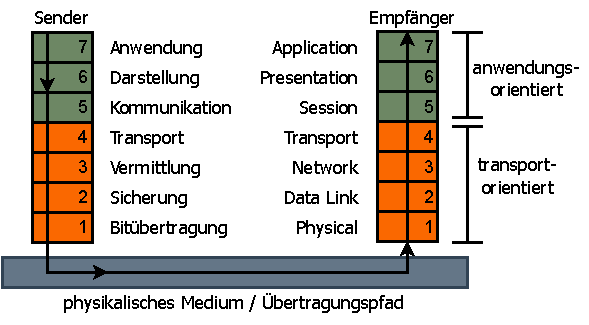
\includegraphics[width=0.7\textwidth]{images/OSI.pdf}
	\caption[OSI-Modell]{Darstellung des ISO/OSI-Modells, das eine standardisierte Kommunikation zwischen einem Sender und einem Empfänger definiert. 
	Beim Sender werden die Schichten des Modells von Anwendung, Darstellung und Kommunikation erst anwendungsorientiert durchlaufen. 
	Danach folgen die Schichten von Transport, Vermittlung, Sicherung und Bitübertragung im transportorientierten Teil. 
	Die Nachricht wird dann über das Medium an den Empfänger geschickt und in genau umgedrehter Reihenfolge entgegengenommen. Angelehnt an \cite{osi-model}.}
	\label{fig:osi_modell}
\end{figure}

\subsection{Die anwendungsorientierten Schichten}

In dieser Untersektion sollen die anwendungsorientierten Schichten des ISO/OSI-Modells näher betrachtet werden. 

Dabei ist die Anwendungsschicht im ISO/OSI-Modell die Schicht, die am nächsten an der Endbenutzer-Interaktion liegt. 
Sie ermöglicht es Anwendungen, auf das Netzwerk zuzugreifen und Dienste zu nutzen. 
Diese Schicht stellt Funktionen wie Identitätsüberprüfung, Zugangskontrolle und Ressourcenallokation zur Verfügung.

Die Darstellungsschicht im ISO/OSI-Modell kümmert sich im Wesentlichen um die Umwandlung der Daten in eine Form, die von der Anwendungsschicht verstanden werden kann. Es geht darum, wie Daten dargestellt, verschlüsselt und komprimiert werden.

Die Kommunikationsschicht spielt im ISO/OSI-Modell eine entscheidende Rolle, da sie den Datentransfer zwischen verschiedenen Netzwerken koordiniert. Sie ist zuständig für verschiedene Funktionen, wie das Routing und die Netzwerkadressierung.

Die genaue Implementierung der Mechanismen aus den anwendungsorientierten Schichten wird im Kapitel~\ref{cha:konzept} vorgestellt. Hier gibt es jedoch einige grundlegende Mechanismen, die betrachtet werden können.

Da die Anwendungsschicht durch die Benutzernähe meist eine hohe Komplexität aufweist, kann es sinnvoll sein, die Mechanismen dieser Schicht auf Mikro- statt auf Nanoebene durchzuführen. 
Am Beispiel eines In-Body-Netzwerkes kann die Aufgabe der Datenverarbeitung und der Ressourcenallokation in einem Body-Area-Netzwerk auf Mikroebene stattfinden, während das In-Body-Netzwerk sich um die niedrigeren Schichten des Modells kümmert. Dass sich unterschiedliche Netzwerktypen und Geräte um unterschiedliche Schichten des ISO/OSI-Modells kümmern, ist auch in herkömmlichen Netzwerken üblich.\cite{osi-model}

Einige Mechanismen der Darstellungsschicht sind analog in der Implementierung von Tile-basierter Self-Assembly 
enthalten. 
Ein DNA-Strang ist eine Sequenz der zwei verschiedenen Basenpaare Adenin/Thymin und Guanin/Cytosin.
So kann in einem offenen DNA-Strang, ähnlich zu einer binären Zahl, Information gespeichert und gelesen werden. Die Information, die am Ende in der Anwendungsschicht ausgelesen und genutzt werden soll, kann so in der Darstellungsschicht in die offenen DNA-Enden \glqq programmiert\grqq\, beziehungsweise codiert werden.

Auch einige Mechanismen der Kommunikationsschicht sind inhärent in Tile-basierten Self-Assemblies vorhanden. So können beispielsweise die offenen DNA-Enden der Liganden mit Adressen gleichgesetzt werden. Denn nur bestimmte Liganden können sich mit bestimmten Rezeptoren des Nachrichtenempfängers verbinden.

Ein möglicher physikalischer Prozess zur Fortbewegung ist die zuvor vorgestellte Diffusion, die beispielsweise in In-Body-Netzwerken durch den Blutfluss erzeugt wird. Andere Optionen könnten die Fortbewegung durch Flagellen oder durch molekulare Motoren sein \cite{lau2020phd}.
Wie die Mechanismen dieser Schichten in DNA-Tile-basierten Nanonetzwerken funktionieren, wird im Kapitel~\ref{cha:konzept} diskutiert. 

\subsection{Die transportorientierten Schichten}

Diese Untersektion beschäftigt sich mit den transportorientierten Schichten des ISO/OSI-Modells. Sie werden in herkömmlichen Kommunikationssystemen meist von unterschiedlichen Netzwerken oder Geräten implementiert. Dementsprechend kann für ein DNA-Tile-basiertes Nanonetzwerk nur schwer definiert werden, auf welcher Schicht der Mechanismus konkret umgesetzt wird.

Die Transportschicht des ISO/OSI-Modells ist für die End-to-End-Kommunikation und die Kontrolle des Datenflusses zwischen zwei Systemen verantwortlich.

Die Vermittlungsschicht, auch bekannt als die Datensicherungsschicht, ist im ISO/OSI-Modell dafür verantwortlich, die Kommunikation zwischen Geräten in einem Netzwerk zu kontrollieren und zu ermöglichen. Sie kümmert sich um Aufgaben wie Framing, physische Adressierung, Flusskontrolle und Fehlerkontrolle.

In der traditionellen Netzwerktechnologie stellt die Sicherungsschicht (Link Layer oder Data Link Layer im ISO/OSI-Modell) sicher, dass Daten sicher und fehlerfrei von einem Knoten zum anderen übertragen werden. Sie ist verantwortlich für die Erkennung und möglicherweise auch für die Korrektur von Fehlern, die auf der physischen Ebene auftreten können.

Die Bitübertragungsschicht, auch bekannt als die physikalische Schicht im ISO/OSI-Modell, ist für die Übertragung von rohen Bitströmen über das physische Medium zuständig. Sie befasst sich mit den technischen Aspekten der Übertragungsmedien wie Verbindungsaufbau, Verbindungstrennung, Modulation und Bitrate.

Wie zuvor angemerkt, verschwimmen die vier transportorientierten Schichten in DNA-Tile-basierten Nanonetzwerken etwas. Mechanismen zur Fehlerkorrektur sind mit dem $k \times k$-Proofreading und dem Snaked-Proofreading in der Sektion~\ref{sec:proofreading} vorgestellt worden. Mechanismen wie die Datenflusskontrolle, Framing, Fehlererkennung oder Modulation, werden im Kapitel~\ref{cha:konzept} näher betrachtet.

Dieses Kapitel hat umfassende Grundlagen von Nanonetzwerken, DNA, Tilebildung, Self-Assembly, Assembly-Modellen, Error-Handling und Kommunikationsmechanismen gebildet und geliefert. Im folgenden Kapitel werden drei Arbeiten näher betrachtet, da diese besondere Nähe zu dieser Arbeit besitzen.

	\chapter{Related Work}
\label{cha:relatedwork}
Dieses Kapitel betrachtet drei wissenschaftliche Publikationen, die dieser Arbeit nahe stehen. Dabei handelt es sich um die Arbeiten \emph{A Deployable Routing System for Nanonetworks} von Liaskos et al., \emph{CORONA: A Coordinate and Routing system for Nanonetworks} von Tsioliaridou et al. und \emph{Hop Count Routing: A Routing Algorithm for Resource Constrained, Identity-Free Medical Nanonetworks} von Büther et al., die alle verschiedene Ansätze für Routing und Koordination von Nanonetzwerken liefern \cite{buether2018hop, tsioliaridou2015corona, liaskos2016routing}. Alle drei Arbeiten wurden kurz im Kapitel~\ref{cha:grundlagen} vorgestellt. In den folgenden Sektionen sollen diese Arbeiten jedoch noch näher betrachtet und vorgestellt werden, da sie von besonderem Interesse für diese Arbeit sind.

\section{Hop Count Routing: A Routing Alogrithm for Resource Constraint, Identity-Free Medical Nanonetworks}

%\section{Hop Count Routing}

Die zuerst betrachtete Arbeit wurde im Jahr 2018 von Florian Büther, Immo Traupe und Sebastian Ebers verfasst \cite{buether2018hop}. Sie wurde mit besonderem Augenmerk auf \emph{In-Body-Networks} (IBN) und \emph{Body-Area-Networks} (BAN) verfasst. Die Nanogeräte in einem solchen Netzwerk unterliegen aufgrund des medizinischen Anwendungsfalls einigen Annahmen. So wird angenommen, dass ein Nanogerät in einem solchen Netzwerk verschiedene Komponenten besitzt: Eine Energieversorgung, eine einfache Recheneinheit, Sensoren und Aktuatoren, die eine aktive Kommunikation über elektromagnetische Terahertzwellen ermöglichen.  Da sich diese Nanogeräte jedoch im menschlichen Körper befinden, können Terahertzwellen nur auf einer Entfernung von ungefähr zwei Millimetern zuverlässig erkannt werden. Aus diesem Grund müssen die Nanogeräte ein Netzwerk aus vielen identischen Einheiten bilden. So kann der Hop-Count genutzt werden, um ein System zu entwickeln, das sowohl in Bezug auf Energie als auch Berechnung effizient ist.
Das in dieser Arbeit vorgestellte Hop-Count-Routing ist Gateway-orientiert. Es gibt ein Gateway auf Mikroebene, das Daten in das Nanonetzwerk sendet oder empfängt. Dabei gibt es zwei Phasen, die zum Routing benötigt werden: die Propagierungsphase und die Routingphase. 

In der Propagierungsphase erhalten alle Nanoknoten im System zu Beginn den Hop-Count $\infty$. Das Gateway sendet eine Nachricht in das Netzwerk mit dem eigenen Hop-Count $0$. Alle Empfängerknoten mit Hop-Count $n_r$ und einer beliebigen Nachricht mit Hop-Count $n_s$ verfahren in der Propagierungsphase wie folgt: Wenn $n_r > n_s + 1$ gilt, dann aktualisiere den eigenen Hop-Count auf $n_s + 1$ und sende den aktualisierten Wert in einer neuen Nachricht im Broadcast weiter. Wenn $n_r \leq n_s + 1$ gilt, dann mache nichts weiter. Da zu Beginn alle Knoten den Hop-Count $\infty$ besitzen, wird jeder Knoten im Netzwerk mindestens einmal aktualisiert und sendet den Hop-Count weiter. Das Ergebnis einer solchen Propagierungsphase ist in Abbildung~\ref{fig:hop-count} zu erkennen. Haben so alle Knoten den minimalen Hop-Count zum Gateway berechnet, so kann die Routingphase durchgeführt werden. 

\begin{figure}
    \centering
    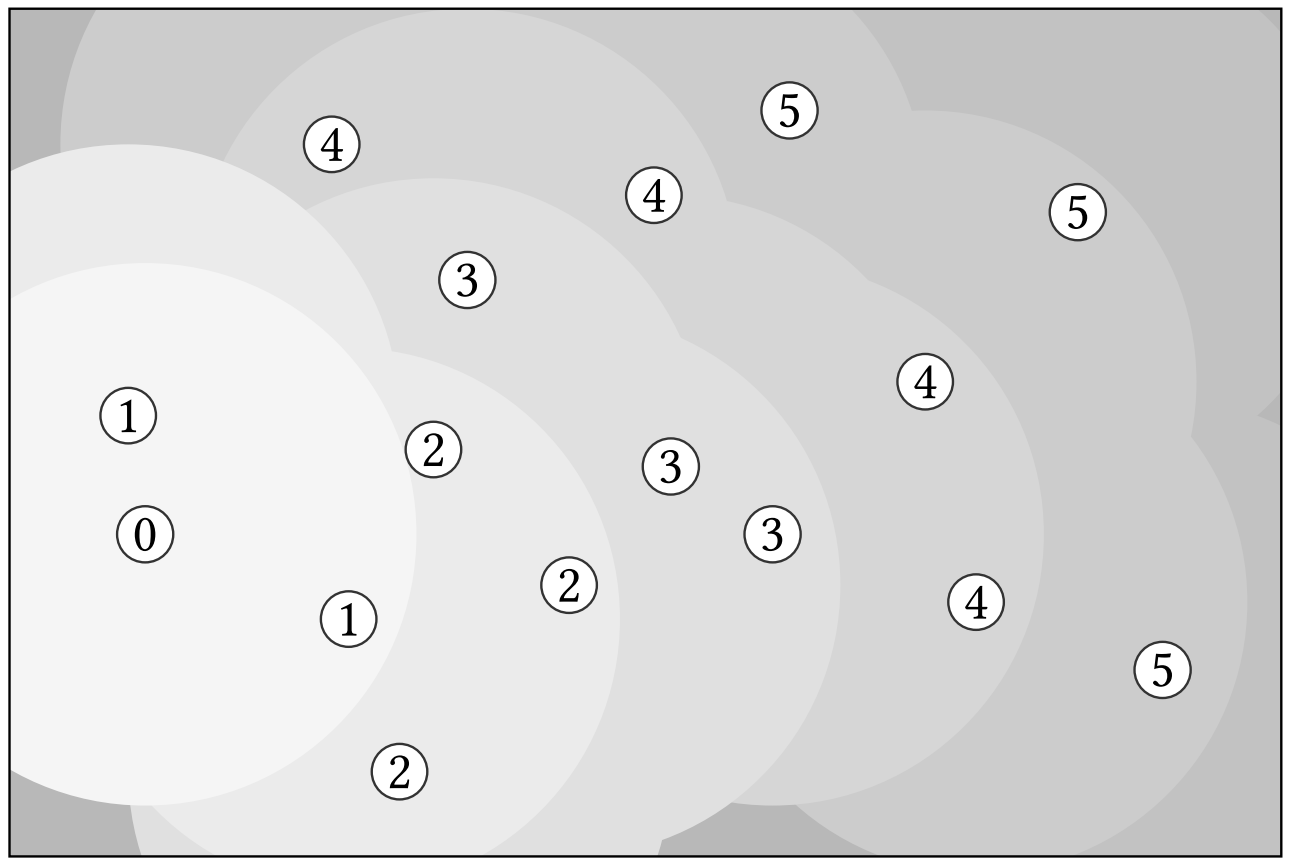
\includegraphics[width=0.65\textwidth]{images/Hop-Count.png}
    \caption[Grafische Darstellung eines gatewayorientierten Hop-Counts]{Grafische Darstellung eines gatewayorientierten Hop-Counts nach der Propagierungsphase. Dabei wird die Reichweite einzelner Knoten durch verschiedene Helligkeitsstufen dargestellt. Die Zahl, mit welcher ein Knoten bezeichnet ist, stellt dabei die Anzahl der Hops zwischen Gateway und Knoten dar.}
    \label{fig:hop-count}
\end{figure}

Während der Routingphase erfolgt eine Unterscheidung zwischen zwei Arten von Nachrichten. Die erste Art umfasst Nachrichten, die von einem Nanoknoten zum Gateway gesendet werden. In diesem Fall muss die Nachricht per Broadcast mit dem aktuellen Hop-Count versehen werden. Alle Knoten überprüfen, wenn sie eine Nachricht empfangen, ob ihr eigener Hop-Count kleiner ist als der in der Nachricht angegebene Hop-Count. Wenn dies der Fall ist, leitet der Knoten die Nachricht mit seinem eigenen Hop-Count weiter. Andernfalls wird nichts weiter unternommen. Die zweite Art von Nachrichten besteht aus Nachrichten, die vom Gateway an einen spezifischen Nanoknoten gesendet werden. In diesem Fall erfolgt eine ähnliche Überprüfung, bei der abgefragt wird, ob der eigene Hop-Count größer ist als der empfangene Hop-Count.

Bei diesem Hop-Count-Routing werden eine große Anzahl von Nanoknoten in jeder Übertragung beteiligt. Eine Optimierung, die diese Überlastung des Netzes verhindern soll, ist die \emph{destruktive Erfassung}. Dabei wird durch Änderung des Hop-Counts sichergestellt, dass alle Knoten nur einmal die Nachricht übertragen. Das führt dazu, dass Nachrichtenübertragungen in einem solchen Netzwerk nur noch sequentiell abläuft und nach einer Nachricht eine neue Propagierungsphase notwendig ist. Dieser Ansatz kann auch dazu führen, dass Übertragungen von Nanoknoten zum Gateway nicht ankommen, da die Knoten um das Gateway herum durch eine Nachricht zuvor genutzt wurden. Eine mögliche Lösung dieses Problems wäre, mehrere Gateways in einem System zu nutzen und alle Knoten den Hop-Count zu jedem Gateway speichern zu lassen. Hier würden aber erhöhte Speicherkosten und weitere Flags in der Nachricht anfallen. 

Bei der Auswertung des naiven und destruktiven Ansatzes für das Hop-Count-Routing kommen die Autoren der Arbeit zu dem Schluss, dass beide Ansätze schnell sind. Auch wenn der destruktive Ansatz eine geringere Nachrichtenmenge benötigt, ist der naive Ansatz ebenfalls einfach und schnell. Der worst-case von $\mathcal{O}(n^2)$ ist in realistischen Implementierungen unwahrscheinlich. Die Laufzeit des Algorithmus ist in der Simulation gut, jedoch wurden einige Annahmen gemacht, die in der Praxis erneut betrachtet werden müssen. In den Simulationen wird angenommen, dass die Nanoknoten statisch immer an derselben Stelle liegen. In einem medizinischen Anwendungsfall, in welchem dieses Netzwerk im menschlichen Körper liegt, ist dies wahrscheinlich nicht der Fall. Außerdem wird beim Modell des Nanoknotens nicht betrachtet, wie viel Zeit die Übertragung und Berechnung im Knoten selbst benötigt.

Abschließend ist zu dieser Arbeit zu sagen, dass ein interessanter und schneller Hop-Count-Routing Algorithmus geliefert wird, der in Hinsicht auf medizinische Body-Area-Networks entwickelt wird. Da einige vereinfachte Annahmen im Modell enthalten sind, muss sich ein solcher Ansatz jedoch noch in einem praxisnäheren Experiment bewähren.

Da sich die Arbeit auf Routing mit Terahertzwellen fokussiert, lässt sich der Algorithmus nicht auf DNA-Tiles und Self-Assemblies übertragen. Das Prinzip eines Body-Area-Networks, das die komplexeren Aufgaben des Netzwerkes übernimmt, ist jedoch interessant in Hinsicht auf die in dieser Masterarbeit betrachteten Nanonetzwerke. Ein Netzwerk auf Mikroebene, das über Gateways Tiles in ein Nanonetzwerk sendet und so mit Nanogeräten und Nanorobotern kommuniziert, stellt ein realistisches Anwendungsbeispiel für DNA-basierte Nanonetzwerke dar.

\section{CORONA: A Coordinate and Routing system for Nanonetworks}

In dieser Arbeit wird das koordinatenbasierte Routing-System CORONA vorgestellt. Das aus dem Jahr 2015 stammende Paper wurde von Ageliki Tsioliaridou, Christos Liaskos, Sotiris Ioannidis und Andreas Pitsillides verfasst \cite{tsioliaridou2015corona}. Das Routing-System basiert auf zwei Annahmen: Das Nanonetzwerk, in welchem es eingesetzt wird, ist vertrauenswürdig und benötigt keine weiteren Sicherheitsmechanismen und die Knoten befinden sich im zweidimensionalen Raum. Auch wird in dieser Arbeit davon ausgegangen, dass ein Knoten in diesem Netzwerk eine Nanomaschine ist, die aus einer Energiequelle, einem Speicher, einer Antenne und einer Recheneinheit besteht. Dabei können alle Knoten autonom einfache Operationen ausführen und über kurze Strecken kommunizieren. 

\begin{figure}
    \centering
    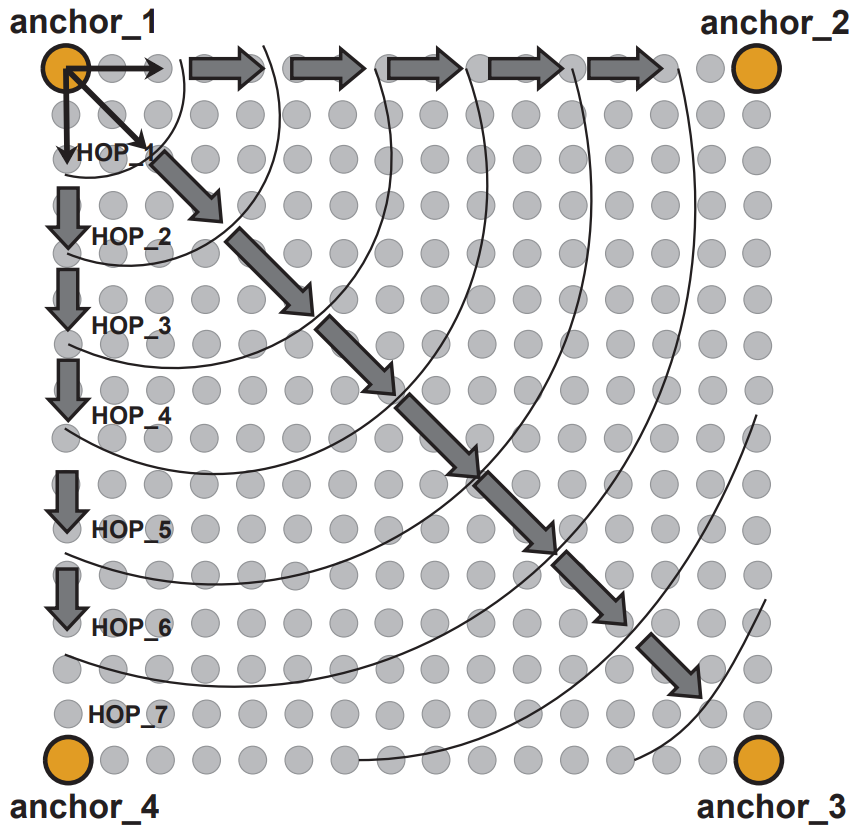
\includegraphics[width=0.5\textwidth]{images/Corona.png}
    \caption[CORONA Ankerpunkte Verbildlichung]{Darstellung eines rechteckigen Gebiets in einem Nanonetzwerk. Die vier Eckpunkte des Gebiets bilden die Ankerpunkte und definieren über die Entfernung zu den einzelnen Knoten über Hops die eindeutigen Positionen jedes Nanoknotens im Gebiet. Abbildung aus der Arbeit von Tsioliaridou et al. \cite{tsioliaridou2015corona}}
    \label{fig:corona}
\end{figure}

Das System basiert auf der Idee, dass Nanonetzwerke in den meisten Anwendungsfällen vorwiegend datenzentriert funktionieren. Ein Ansatz aus einer früheren Arbeit, der einen wiederholten Broadcast aller Nachrichten durchführt, soll in dieser Arbeit durch ein Unicast-basiertes System ersetzt werden \cite{liaskos2015flood}. Die Arbeit legt den Fokus bei Nanomaschinen auf \emph{Software-Defined Metamaterials} (SDM), einer neuen Klasse von künstlichen Materialien mit programmierbaren elektromagnetischen Eigenschaften \cite{liaskos2015sdm}. Mit diesen Grundlagen werden in einem rechteckigen Gebiet Nanoknoten platziert. Die vier Ecken des Rechtecks werden dabei als Ankerpunkte definiert. Auf Basis von Standard-Triangulation können so allen Nanoknoten in diesem Gebiet eindeutige Koordinaten gegeben werden, indem die Entfernung über Hops zwischen dem Knoten und den Ankerpunkten definiert wird. Dieser Vorgang wird während der Einrichtungsphase einmalig durchgeführt. Das System ist in Abbildung~\ref{fig:corona} beispielhaft dargestellt. 

Da sich das System im zweidimensionalen Raum befindet und die vier Ankerpunkte an den Eckpunkten des Gebietes liegen, reichen die zwei nächsten Ankerpunkte, um durch Triangulation die genaue Position eines Knotens zu definieren. Jede andere mögliche Position wäre außerhalb des Gebietes. Bei der Übertragung eines Pakets von einem Senderknoten zu einem Empfängerknoten entscheidet der Senderknoten basierend auf der geringsten Anzahl von Hops, welches Ankerpunktpaar für das Routing verwendet werden soll. Die Übertragung einer Nachricht von einem Senderknoten $S$ mit den Koordinaten $(s_1, s_2, s_3, s_4)$ zu einem Empfängerknoten $R$ mit den Koordinaten $(r_1, r_2, r_3, r_4)$ läuft so wie folgt ab: Der Senderknoten wählt das passende Ankerpaar $(anchor_i, anchor_j)$ anhand von $s_k, k\in\{1,2,3,4\}$ aus. Von diesem Ankerpaar wird auch die Position des Empfängers definiert. Das zu übertragende Paket wird wie bei einem Broadcast versendet, jedoch gibt es einen Mechanismus, durch welchen der Broadcast durch das gesamte System verhindert wird.
Ein Knoten T mit den Koordinaten $(t_1, t_2, t_3, t_4)$ muss beim Erhalten des Paketes einen Vergleich durchführen:
\begin{align*}
    (t_i \in [s_i, r_i]) \&\& (t_j \in [s_j , r_j ]) 
\end{align*}
Dabei wird im Endeffekt nur überprüft, ob der Knoten $T$ innerhalb des Gebietes ist, das von den Ankerpunkten aufgespannt wird. Ist dies nicht der Fall, so wird das Paket nicht weitergeleitet.
Wenn so die Ankerpunkte für eine Übertragung zwischen $S$ und $R$ gut gewählt sind, kann die Übertragung durchgeführt werden, ohne dabei das gesamte System mit einem Broadcast zu fluten. In den Simulationen der Arbeit konnte gezeigt werden, dass CORONA im Vergleich zu alternativen Lösungen kürzere Paketpfade bietet.

Schlussfolgernd lässt sich zu CORONA sagen, dass es gute Verbesserungen und Optimierungen für das Routing in Nanonetzwerken geliefert hat. Jedoch funktioniert dieser Ansatz bislang nur im zweidimensionalen Raum und lässt sich in Bezug auf diese Masterarbeit schwer übertragen. Ein bedeutender Grund dafür ist, dass sich diese Arbeit mit SDMs statt DNA-Tiles befasst. Deshalb ist das Routing nicht in DNA-Tile-basierten Nanonetzwerken anwendbar.

\section{A Deployable Routing System for Nanonetworks}

Diese Arbeit wurde im Jahr 2015 von Christos Liaskos, Ageliki Tsioliaridou, Andreas Pitsillides, Ian F. Akyildiz, Nikolaos V. Kantartzis, Antonios X. Lalas, Xenofontas Dimitropoulos, Sotiris Ioannidis Maria Kafesaki und C.M. Soukoulis verfasst \cite{liaskos2015sdm}. Das \emph{Deployable Routing System} (DEROUS) für ad-hoc-Nanonetzwerk nimmt genau wie das CORONA auch SDMs an. DEROUS basiert auf dem Konzept eines Beacons, um den herum dynamisch kreisförmige und radiale Routingpfade geformt werden. Wie auch CORONA setzt es auf eine zweidimensionale Topologie. Es wird angenommen, dass die Nanoknoten Nachrichten drahtlos in zwei unterschiedlichen Modi übertragen können: Im Low-Power-Modus mit geringer Reichweite und niedrigem Energieverbrauch sowie im normalen Modus mit größerem Radius und höherem Energieverbrauch.

Der Vorgang bei DEROUS ist in zwei Phasen unterteilt: die Einsatzphase und die Datenroutingphase. Die Einsatzphase ist eine kurze Phase zum Initialisieren des Systems. Dabei wird extern ein Nanoknoten als Beacon-Point festgelegt. Dieser sendet ein Paket im Broadcast zuerst im Low-Power Modus aus. Dabei wird durch Hop-Count und ein spezifisches Flag die Entfernung jedes Knotens zum Beacon lokal bei jedem Knoten festgehalten. Der gleiche Vorgang wird danach noch einmal im normalen Modus durchgeführt. Alle Knoten speichern dadurch die Hop-Count-Entfernung von beiden Modi. Ist die Einsatzphase abgeschlossen, können sowohl im Low-Power als auch im normalen Modus Nachrichten zwischen einem Sender und Empfänger gesendet werden. Dabei wird lediglich die Entfernung von Sender und Empfänger zum Beacon-Point benötigt. In der Datenroutingphase sendet der Sender $S$ ein Paket mit seiner Entfernung und der Entfernung des Empfängers zum Empfänger $R$. Dies wird wieder mit einem Broadcast gemacht, jedoch leitet ein Nanoknoten $T$ nur die Nachricht weiter, wenn eine der folgenden Voraussetzungen eingehalten ist:
\begin{align*}
    (1)& HC_S \leq HC_T \leq HC_R \land HC_S \leq HC_R\\
    (2)& HC_R < HC_T < HC_S, \land HC_R < HC_S
\end{align*}
Dabei ist $HC_X$ die Entfernung beziehungsweise der Hop-Count des Beacon zum Knoten $X$. Diese Bedingungen besagen, dass alle Knoten zwischen Sender $S$ und Empfänger $R$, die auf dem Ring um den Beacon liegen, die Nachricht weiterleiten. Dies ist in Abbildung~\ref{fig:derous} zu erkennen.

\begin{figure}
    \centering
    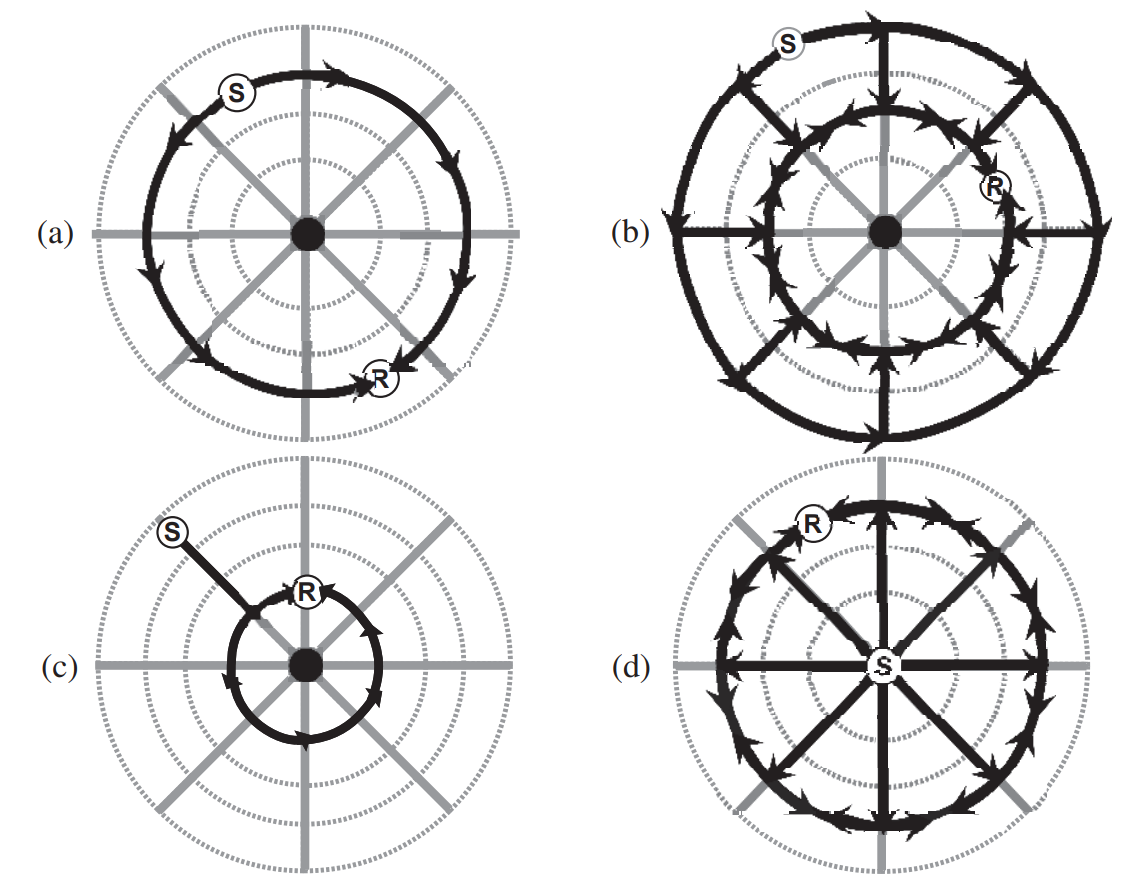
\includegraphics[width=0.75\textwidth]{images/Derous.png}
    \caption[DEROUS Protokoll Szenarien]{Darstellung von vier (a-d) verschiedenen Routing Szenarien nach dem DEROUS-Protokoll. Die schwarzen Pfeile stellen dabei die Wege dar, die ein verschicktes Paket zwischen Sender S und Empfänger R nehmen kann. \cite{liaskos2015sdm}}
    \label{fig:derous}
\end{figure}

Im Vergleich zu CORONA und anderen Routing-Systemen auf Nanoebene schneidet DEROUS gut ab. Es verringert die Anzahl von wiederholten Übertragungen und hat eine hohe Rate erfolgreicher Peer-to-Peer Übertragungen. Auch schneidet es im Vergleich zu anderen Protokollen gut ab, wenn es um die Flutungsrate geht. Dabei geht es darum, wie viel im Durchschnitt geflutet wird. Diese Rate ist in DEROUS abhängig davon, wo der Beacon gesetzt ist, jedoch sind auch worst case Szenarien noch besser als einige andere Ansätze.

Zusammenfassend lässt sich sagen, dass DEROUS einen vielversprechendes Ansatz für ad-hoc Nanonetzwerke bietet. Dabei ist es sowohl für Low-Power-Anwendungen als auch für Anwendungen mit höherem Energiebedarf geeignet. Obwohl die Betrachtung von DEROUS, ähnlich wie bei CORONA, momentan auf den zweidimensionalen Raum beschränkt ist, kann DEROUS mit relativ geringem Aufwand auf einen dreidimensionalen Raum erweitert werden. In diesem Fall würde die Kommunikation nicht radial oder kreisförmig, sondern sphärisch ablaufen.

Aus allen drei vorgestellten Arbeiten lässt sich ableiten, dass Kommunikationsprotokolle für DNA-basierten Nanonetzwerken in keiner Arbeit konkret betrachtet werden. Die meisten Arbeiten für Nanonetzwerke konzentrieren sich auf andere Materialien oder Mechanismen. Diese können als Inspiration für DNA-Tiles verwendet werden, jedoch lässt sich wegen der Eigenschaften der benutzen Materialien keines der Routing Protokolle komplett auf Nanonetzwerke mit DNA-basierter Self-Assembly übersetzen.
Nach der Betrachtung der verwandten Arbeiten und den zuvor gelegten Grundlagen kann im Folgenden das Konzept vorgestellt werden.

	\chapter{Konzeption}
\label{cha:konzept}
In diesem Kapitel wird ein Konzept vorgestellt, das alle in dieser Arbeit besprochenen Mechanismen und Anforderungen herkömmlicher Kommunikationsprotokolle umfasst. Die Anforderungen werden zunächst in drei Hauptkategorien eingeteilt:
\begin{itemize}
\item Anforderungen, die inhärent in der Ausführung von Self-Assembly durch DNA-Tiles sind,
\item Anforderungen, die speziell für die Kommunikation mit DNA-Tile-basierten Systemen definiert werden müssen,
\item Anforderungen, die auf der Nanoebene nicht umgesetzt werden sollten, da sie sich besser für eine Implementierung auf einer anderen Ebene eignen.
\end{itemize}
In den folgenden Sektionen werden diese Arten von Anforderungen besprochen und vorgestellt. Dazu gehören die Adressierung, das Übertragungsmedium, Routing, Dialogaufbau, Fehlererkennung, Fehlerkorrektur, Framing, Datenflusskontrolle, Nachrichtencodierung und Flags. Abschließend werden einige dieser Mechanismen in einem Beispiel zusammengefasst und im ISO/OSI-Modell eingeordnet.

\section{Die Adressierung in Nanonetzwerken}

\begin{figure}
    \centering 
    \begin{tikzpicture}[scale=0.87]
        % Südliche Verbindung Shapes
        \draw[fill=uzl_red_3] (7.1,-0.5) rectangle (8.3,2.9);
        \buildBaseA{0}{0}
        \buildBaseC{1.2}{0}
        \buildBaseT{2.4}{0}
        \buildBaseG{3.6}{0}
        \buildBaseA{4.8}{0}
        \buildBaseC{6}{0}
        \buildBaseA{7.2}{0}
        \buildBaseT{8.4}{0}
        \buildBaseC{9.6}{0}
        \buildBaseT[down]{0}{1.2}
        \buildBaseG[down]{1.2}{1.2}
        \buildBaseA[down]{2.4}{1.2}
        \buildBaseC[down]{3.6}{1.2}
        \buildBaseT[down]{4.8}{2.4}
        \buildBaseG[down]{6}{2.4}
        \buildBaseC[down]{7.2}{2.4}
        \buildBaseA[down]{8.4}{2.4}
        \buildBaseG[down]{9.6}{2.4}
        \buildBaseG[down]{10.8}{2.4}
        \buildBaseA[down]{12}{2.4}
        \buildBaseC[down]{13.2}{2.4}
        \buildBaseG[down]{14.4}{2.4}
        \buildBaseC{10.8}{1.2}
        \buildBaseT{12}{1.2}
        \buildBaseG{13.2}{1.2}
        \buildBaseC{14.4}{1.2}
        \draw[line width=3pt] (-0.2,0) -- (10.7,0);
        \draw[line width=3pt] (-0.2,1.2) -- (4.7,1.2);
        \draw[line width=3pt] (10.7,1.2) -- (15.5,1.2);
        \draw[line width=3pt] (4.7,2.4) -- (15.5,2.4);
        % Südliche Verbindung Bezeichner
        \node at (-0.5,1.2) {b)};
        \node at (0.5,-0.3) {AT};
        \node at (1.7,-0.3) {CG};
        \node at (2.9,-0.3) {TA};
        \node at (4.1,-0.3) {GC};
        \node at (5.3,-0.3) {A};
        \node at (6.5,-0.3) {C};
        \node[text=white] at (7.7,-0.3) {A};
        \node at (8.9,-0.3) {T};
        \node at (10.1,-0.3) {C};
        \node at (11.3,0.9) {CG};
        \node at (12.5,0.9) {TA};
        \node at (13.7,0.9) {GC};
        \node at (14.9,0.9) {CG};
        \node at (5.3,0.9) {1};
        \node at (6.5,0.9) {2};
        \node[text=white] at (7.7,0.9) {1};
        \node at (8.9,0.9) {0};
        \node at (10.1,0.9) {2};
        \node at (5.3,1.5) {T};
        \node at (6.5,1.5) {G};
        \node[text=white] at (7.7,1.5) {C};
        \node at (8.9,1.5) {A};
        \node at (10.1,1.5) {G};
        \node at (0.5,1.5) {1};
        \node at (1.7,1.5) {2};
        \node at (2.9,1.5) {0};
        \node at (4.1,1.5) {3};
        \node at (5.3,2.7) {1};
        \node at (6.5,2.7) {2};
        \node[text=white] at (7.7,2.7) {3};
        \node at (8.9,2.7) {0};
        \node at (10.1,2.7) {2};
        \node at (11.3,2.7) {2};
        \node at (12.5,2.7) {0};
        \node at (13.7,2.7) {3};
        \node at (14.9,2.7) {2};
        %
        %
        % Nördliche Verbindung Shapes
        \buildBaseA{0}{3.9}
        \buildBaseA{1.2}{3.9}
        \buildBaseC{2.4}{3.9}
        \buildBaseT{3.6}{3.9}
        \buildBaseC{4.8}{3.9}
        \buildBaseA{6}{3.9}
        \buildBaseA{7.2}{3.9}
        \buildBaseG{8.4}{3.9}
        \buildBaseT{9.6}{3.9}
        \buildBaseT[down]{0}{5.1}
        \buildBaseT[down]{1.2}{5.1}
        \buildBaseG[down]{2.4}{5.1}
        \buildBaseA[down]{3.6}{5.1}
        \buildBaseG[down]{4.8}{6.3}
        \buildBaseT[down]{6}{6.3}
        \buildBaseT[down]{7.2}{6.3}
        \buildBaseC[down]{8.4}{6.3}
        \buildBaseA[down]{9.6}{6.3}
        \buildBaseA[down]{10.8}{6.3}
        \buildBaseG[down]{12}{6.3}
        \buildBaseC[down]{13.2}{6.3}
        \buildBaseT[down]{14.4}{6.3}
        \buildBaseT{10.8}{5.1}
        \buildBaseC{12}{5.1}
        \buildBaseG{13.2}{5.1}
        \buildBaseA{14.4}{5.1}
        \draw[line width=3pt] (-0.2,3.9) -- (10.7,3.9);
        \draw[line width=3pt] (-0.2,5.1) -- (4.7,5.1);
        \draw[line width=3pt] (10.7,5.1) -- (15.5,5.1);
        \draw[line width=3pt] (4.7,6.3) -- (15.5,6.3);
        % Nördliche Verbindung Bezeichner
        \node at (-0.5,5.1) {a)};
        \node at (0.5,3.6) {AT};
        \node at (1.7,3.6) {AT};
        \node at (2.9,3.6) {CG};
        \node at (4.1,3.6) {TA};
        \node at (5.3,3.6) {C};
        \node at (6.5,3.6) {A};
        \node at (7.7,3.6) {A};
        \node at (8.9,3.6) {G};
        \node at (10.1,3.6) {T};
        \node at (11.3,4.8) {TA};
        \node at (12.5,4.8) {CG};
        \node at (13.7,4.8) {GC};
        \node at (14.9,4.8) {AT};
        \node at (5.3,4.8) {2};
        \node at (6.5,4.8) {1};
        \node at (7.7,4.8) {1};
        \node at (8.9,4.8) {3};
        \node at (10.1,4.8) {0};
        \node at (5.3,5.4) {G};
        \node at (6.5,5.4) {T};
        \node at (7.7,5.4) {T};
        \node at (8.9,5.4) {C};
        \node at (10.1,5.4) {A};
        \node at (0.5,5.4) {1};
        \node at (1.7,5.4) {1};
        \node at (2.9,5.4) {2};
        \node at (4.1,5.4) {0};
        \node at (5.3,6.6) {2};
        \node at (6.5,6.6) {1};
        \node at (7.7,6.6) {1};
        \node at (8.9,6.6) {3};
        \node at (10.1,6.6) {0};
        \node at (11.3,6.6) {0};
        \node at (12.5,6.6) {2};
        \node at (13.7,6.6) {3};
        \node at (14.9,6.6) {1};
    \end{tikzpicture}
    \caption[Konzeptionelle Darstellung offener DNA-Stränge]{Konzeptionelle Darstellung von offenen DNA-Strängen und der möglichen Codierung der Basenpaare zur Adressierung. In a) verbinden sich die Stränge mit der Adresse 03112, in b) verbinden sich die Stränge nicht, da verschiedene Adressen vorhanden sind (20121 und 20321).}
    \label{fig:dna_adressierung}
\end{figure}

Das zuerst betrachtete Konzept ist in DNA-Tile basierten Systemen inhärent. Die Adressierung von Nanogeräten muss nicht weiter implementiert werden. Kommunikation zwischen zwei Geräten funktioniert durch Verbindung der Liganden des Nachrichtenmoleküls an den Rezeptoren des Empfängergerätes. Dieser Mechanismus kann für die Adressierung genutzt werden. Wie in Abbildung~\ref{fig:dna_adressierung} zu erkennen ist, können die Basenpaare für die Adressierung codiert werden. Im gegebenen Beispiel könnte die Codierung beispielsweise wie folgt aus:
\begin{align*}
    TA &= \text{ Empfänger } T = \text{ Sender } A = 0 = 00\\
    AT &= \text{ Empfänger } A = \text{ Sender } T = 1 = 01\\
    CG &= \text{ Empfänger } C = \text{ Sender } G = 2 = 10\\
    GC &= \text{ Empfänger } G = \text{ Sender } C = 3 = 11\\
\end{align*}
Die offenen Enden der DNA-Stränge können auf diese Weise als Adressen codiert werden. In diesem Beispiel in a) kann so die Adresse 03112 dargestellt werden. In b) verbinden sich die offenen Enden nicht, da Adenin und Cytosin kein Basenpaar bilden können. Somit sind auch die Adressen unterschiedlich (20121 und 20321). Um Adressierung in DNA-Tile-basierten Nanonetzwerken zu realisieren, muss somit kein weiterer Mechanismus entworfen werden. 

\section{Das Übertragungsmedium in Nanonetzwerken}

Eine speziell in funkbasierten Netzwerken bedeutsame Anforderung betrifft die Auswahl des Übertragungsmediums. In DNA-Tile-basierten Nanonetzwerken ist das Übertragungsmedium im Anwendungsgebiet definiert. Da in dieser Arbeit besonderes Augenmerk auf die medizinische Anwendung gelegt wird, kann das Übertragungsmedium hier als der Blutkreislauf eines Menschen gesehen werden. Durch den Blutstrom und Diffusion bewegen sich so alle Geräte im System, was eine Anforderung für die Nanogeräte direkt abdeckt. Die Nanogeräte benötigen so keine externe Fortbewegungsmethode wie Nanomotoren oder ähnliche Ansätze. Andere Übertragungsmedien in anderen Anwendungsfällen sind jedoch denkbar.

\section{Routing und Dialogaufbau in Nanonetzwerken}

Zwei weitere Anforderungen von herkömmlichen Kommunikationsprotokollen ist das Routing und der Dialogaufbau zwischen einzelnen oder mehreren Geräten. Beide sind in DNA-Tile-basierten Nanonetzwerken von niedriger Priorität. Auf einem so kleinen Skalenbereich ist es schwierig, einen Dialog zwischen Teilnehmern des Systems aufzubauen. Es ist in einem solchen Kontext sinnvoll, die Nachrichten und die Kommunikation auf ein Minimum zu beschränken. Bedeutend ist dabei die schnelle Übertragung von Informationen mit geringem Overhead. Obwohl das Routing eine zentrale Anforderung in herkömmlichen Kommunikationsprotokollen ist, hat es in DNA-Tile-basierten Nanonetzwerken eine geringere Relevanz, da die meisten Szenarien ohne Routing auskommen. Da sich alle Nachrichten in einem solchen System zufällig oder durch den Blutkreislauf durch das gesamte System bewegen, muss die Nachricht nicht von anderen Teilnehmern geroutet werden. Da auch die Adressierung, wie vorgestellt wurde, durch Liganden und Rezeptoren abgebildet ist, muss kein Routing vollzogen werden. Hierbei unterscheidet sich ein Nanonetzwerk basierend auf DNA-Tiles und Self-Assembly stark von anderen Nanonetzwerken. Die im Kapitel~\ref{cha:relatedwork} vorgestellten Netzwerke benötigen beispielsweise alle eine Form des Routings, um Kommunikation zu ermöglichen. 

\section{Framing in Nanonetzwerken}

\begin{figure}
    \centering
    \begin{tikzpicture}[scale=1.1]
        \begin{scope}[on background layer]
            % Paket 1 Hintergrund
            \draw[fill=uzl_gray_2] (0.8,-2) rectangle (-2,2);
            % Paket 2a Hintergrund
            \draw[fill=uzl_gray_2] (-2.6,0.4) rectangle (-6.6,4.4);
            % Paket 2b Hintergrund
            \draw[fill=uzl_gray_2] (-2.6,-4.4) rectangle (-6.6,-0.4);
            % Paket 3a Hintergrund
            \draw[fill=uzl_gray_2] (-7.2,0.4) rectangle (-10,4.4);
            % Paket 3b Hintergrund
            \draw[fill=uzl_gray_2] (-7.2,-4.4) rectangle (-10,-0.4);
        \end{scope}
        % Paket e
        \node at (-0.6,2.3) {c)};
        \tileEQsnakedA{0}{1.2}
        \tileEQsnakedSigma{0}{0}
        \tileEQsnakedB{0}{-1.2}
        %
        \tileEQsnakedU{-1.2}{1.2}
        \tileEQsnakedE{-1.2}{0}
        \tileEQsnakedY{-1.2}{-1.2}
        %
        % Paket b
        %
        \node at (-4.6,4.7) {b)};
        \tileEQsnakedV{-3.4}{3.6}
        \tileEQsnakedE{-3.4}{2.4}
        \tileEQsnakedZ{-3.4}{1.2}
        %
        \tileEQsnakedW{-4.6}{3.6}
        \tileEQsnakedF{-4.6}{2.4}
        \tileEQsnakedEinskorrekt{-4.6}{1.2}
        %
        \tileEQsnakedX{-5.8}{3.6}
        \tileEQsnakedF{-5.8}{2.4}
        \tileEQsnakedZwei{-5.8}{1.2}
        %
        % Paket d
        %
        \node at (-4.6,-0.1) {e)};
        \tileEQsnakedV{-3.4}{-1.2}
        \tileEQsnakedL{-3.4}{-2.4}
        \tileEQsnakedZ{-3.4}{-3.6}
        %
        \tileEQsnakedW{-4.6}{-1.2}
        \tileEQsnakedJ{-4.6}{-2.4}
        \tileEQsnakedEins{-4.6}{-3.6}
        %
        \tileEQsnakedX{-5.8}{-1.2}
        \tileEQsnakedK{-5.8}{-2.4}
        \tileEQsnakedZwei{-5.8}{-3.6}
        %
        % Paket a
        %
        \node at (-8.6,4.7) {a)};
        \tileEQsnakedC{-8}{3.6}
        \tileEQsnakedT{-8}{2.4}
        \tileEQsnakedD{-8}{1.2}
        %
        \tileEQsnakedP{-9.2}{3.6}
        \tileEQsnakedR{-9.2}{2.4}
        \tileEQsnakedO{-9.2}{1.2}
        %
        % Paket c
        %
        \node at (-8.6,-0.1) {d)};
        \tileEQsnakedC{-8}{-1.2}
        \tileEQsnakedS{-8}{-2.4}
        \tileEQsnakedD{-8}{-3.6}
        %
        \tileEQsnakedN{-9.2}{-1.2}
        \tileEQsnakedQ{-9.2}{-2.4}
        \tileEQsnakedM{-9.2}{-3.6}
    \end{tikzpicture}
    \caption[Framing Problem Beispiel]{Beispielhafte Aufteilung eines Nachrichtenmoleküls in drei Teile. Die grauen Boxen verdeutlichen dabei, welche Tile-Assemblies ein Frame bilden. Dabei kann an den Kleberbezeichnern erkannt werden, dass die Frames a), b) und c) das korrekte Molekül bilden. Jedoch können sich Frame a) oder d) gleichermaßen an den Rezeptoren eines Empfängers binden. Im Fall d) würde sich e) weiter binden und bei Temperatur drei auch Frame c). Dies würde jedoch zu einem Growth-Error zwischen den Tiles \emph{E} und \emph{L} führen. Auch ist in dieser Abbildung durch die Farbkodierung zu erkennen, dass durch die Tiles \emph{A,B,P} und \texttt{O} bereits eine Art Frame vorhanden ist.}
    \label{fig:framing}
\end{figure}

Ein Verfahren, um die Paketgröße von Nachrichten zu reduzieren und somit größere Datenmengen effizient verarbeiten zu können, ist das \emph{Framing}. Framing hat in herkömmlichen Kommunikationsprotokollen großen Nutzen, in Nanonetzwerken ist Framing im Verhalten der Tile-basierten Self-Assembly enthalten. Mit der Seed-Assembly und den möglicherweise vorhandenen Tiles nördlich und südlich der Seed-Assembly kann der Frameanfang definiert werden. Die Liganden im Tileset bilden das Ende des Frames. Zusätzlich implementiertes Framing innerhalb einer Self-Assembly ist jedoch oft nicht sinnvoll. Obwohl das Aufteilen eines Nachrichtenmoleküls in mehrere kleinere Moleküle interessant und sinnvoll erscheinen mag, werden Tilesets so designt, dass sie sich kontrolliert und spezifisch bilden.

Um das Problem klarer zu machen, findet sich ein Beispiel in Abbildung~\ref{fig:framing}. Dafür wird eine Self-Assembly für den binären Äquivalenzvergleich verwendet. Dabei wird die Information, ob die Binärzahlen äquivalent sind, vom Seedtile bis zum linken Ende des Moleküls weitergegeben. Solange die beiden Binärzahlen im inneren Kleber der nördlichen und südlichen Grenze des Moleküls äquivalent sind, wird ein \emph{k} im horizontal im Moleküls weitergegeben. Sobald sich zwei Binärstellen unterscheiden, wird statt dem \emph{k} ein \emph{n} weitergegeben. In Abbildung~\ref{fig:framing} ist a), b) und c) das korrekt gebundene Molekül. Jedoch kann sich auch d) und e) gemeinsam an den Rezeptoren eines potenziellen Empfängers binden. Das Tileset ist auf Temperatur drei ausgelegt, dementsprechend kann sich auch c) an e) binden, obwohl der innere Kleber mit \emph{k} und \emph{n} unterschiedlich ist. Somit würde sich das Molekül mit einem Growth-Error falsch binden. Nur in Self-Assemblies, die keine Information horizontal in der Self-Assembly weitergeben, könnte Framing angewendet werden.

Framing kann also für speziell dafür definierte Tilesets angewandt werden. Soll Framing in Nanonetzwerken angewendet werden, so bietet es sich an, mehrere kleinere Tilesets zu bilden, die sich untereinander an den Liganden verbinden können. Die Idee wird in Abbildung~\ref{fig:framing_idee} skizziert, jedoch wird sie in dieser Arbeit nicht weiter behandelt, da die Umsetzung eines solchen Prozesses weitere Definitionen benötigt, die den Rahmen dieser Arbeit überschreiten würden. 

Bisher benötigen die vorgestellten Anforderungen keine zusätzlichen Mechanismen für ihre Implementierung in DNA-Tile-basierten Nanonetzwerken. Lediglich beim Framing wurde eine Idee präsentiert, die weiteres Eingreifen erfordert. Im Gegensatz dazu müssen die folgenden Anforderungen implementiert werden, da sie nicht bereits durch die inhärenten Mechanismen der DNA-Tile-basierten Tile-Assembly abgedeckt sind.

\begin{figure}
    \centering
    \begin{tikzpicture}
        \node[scale=0.96, draw, rotate=90] at (-1.8,1.85) {Nanogerät};
        \draw (-1,2.8) -- (-1.51,2.8);
        \draw (-1.51,0.9) -- (-1,0.9);
        %
        \draw[fill=black] (0.2,2.7) rectangle (0.3,2.8);
        \draw (0.33,2.83) -- (0.45,2.95);
        \node at (0.6,3) {L};
        %
        \draw[fill=black] (-1.2,2.7) rectangle (-1.3,2.8);
        \draw (-1.17,2.67) -- (-1.05,2.54);
        \node at (-0.9,2.49) {R};
        %
        \draw[fill=black] (-1.2,1) rectangle (-1.3,0.9);
        \draw (-1.17,1.03) -- (-1.05,1.15);
        \node at (-0.9,1.2) {R};
        %
        \draw[fill=uzl_red_3] (0,2.2) rectangle (0.5,2.7);
        \draw[fill=uzl_red_2] (0.6,2.2) rectangle (1.1,2.7);
        \draw[fill=uzl_red_2] (1.2,2.2) rectangle (1.7,2.7);
        \draw[fill=uzl_red_2] (1.8,2.2) rectangle (2.3,2.7);
        \draw[fill=uzl_red_2] (2.4,2.2) rectangle (2.9,2.7);
        \draw[fill=uzl_red_2] (3,2.2) rectangle (3.5,2.7);
        \draw[fill=uzl_red_2] (3.6,2.2) rectangle (4.1,2.7);
        \draw[fill=uzl_red_2] (4.2,2.2) rectangle (4.7,2.7);
        \draw[fill=uzl_red_2] (4.8,2.2) rectangle (5.3,2.7);
        \draw[fill=uzl_red_2] (5.4,2.2) rectangle (5.9,2.7);
        \draw[fill=uzl_red_2] (6,2.2) rectangle (6.5,2.7);
        \draw[fill=uzl_red_1] (6.6,2.2) rectangle (7.1,2.7);
        %
        \draw (0,1.6) rectangle (0.5,2.1);
        \node at (0.25,1.85) {K};
        \draw (0.6,1.6) rectangle (1.1,2.1);
        \node at (0.85,1.85) {J};
        \draw (1.2,1.6) rectangle (1.7,2.1);
        \node at (1.45,1.85) {I};
        \draw (1.8,1.6) rectangle (2.3,2.1);
        \node at (2.05,1.85) {H};
        \draw (2.4,1.6) rectangle (2.9,2.1);
        \node at (2.65,1.85) {G};
        \draw (3,1.6) rectangle (3.5,2.1);
        \node at (3.25,1.85) {F};
        \draw (3.6,1.6) rectangle (4.1,2.1);
        \node at (3.85,1.85) {E};
        \draw (4.2,1.6) rectangle (4.7,2.1);
        \node at (4.45,1.85) {D};
        \draw (4.8,1.6) rectangle (5.3,2.1);
        \node at (5.05,1.85) {C};
        \draw (5.4,1.6) rectangle (5.9,2.1);
        \node at (5.65,1.85) {B};
        \draw (6,1.6) rectangle (6.5,2.1);
        \node at (6.25,1.85) {A};
        \draw[fill=uzl_yellow_1] (6.6,1.6) rectangle (7.1,2.1);
        %
        \draw[fill=uzl_mediumblue_3] (0,1) rectangle (0.5,1.5);
        \draw[fill=black] (0.2,1) rectangle (0.3,0.9);
        \draw (0.33,0.87) -- (0.45,0.75);
        \node at (0.6,0.7) {L};
        \draw[fill=uzl_mediumblue_2] (0.6,1) rectangle (1.1,1.5);
        \draw[fill=uzl_mediumblue_2] (1.2,1) rectangle (1.7,1.5);
        \draw[fill=uzl_mediumblue_2] (1.8,1) rectangle (2.3,1.5);
        \draw[fill=uzl_mediumblue_2] (2.4,1) rectangle (2.9,1.5);
        \draw[fill=uzl_mediumblue_2] (3,1) rectangle (3.5,1.5);
        \draw[fill=uzl_mediumblue_2] (3.6,1) rectangle (4.1,1.5);
        \draw[fill=uzl_mediumblue_2] (4.2,1) rectangle (4.7,1.5);
        \draw[fill=uzl_mediumblue_2] (4.8,1) rectangle (5.3,1.5);
        \draw[fill=uzl_mediumblue_2] (5.4,1) rectangle (5.9,1.5);
        \draw[fill=uzl_mediumblue_2] (6,1) rectangle (6.5,1.5);
        \draw[fill=uzl_mediumblue_1] (6.6,1) rectangle (7.1,1.5);
        %
        %
        %
        \node[scale = 1.5] at (3.55,0.3) {$\Downarrow$};
        %
        %
        %
        \draw (-3.4,-0.9) -- (-3.91,-0.9);
        \draw (-3.91,-2.8) -- (-3.4,-2.8);
        %
        \node[scale=0.96, draw, rotate=90] at (-4.2,-1.85) {Nanogerät};
        \draw[fill=black] (-3.6,-1) rectangle (-3.7,-0.9);
        \draw (-3.57,-1.03) -- (-3.45,-1.15);
        \node at (-3.3,-1.25) {R};
        %
        \draw[fill=black] (-3.6,-2.7) rectangle (-3.7,-2.8);
        \draw (-3.57,-2.67) -- (-3.45,-2.55);
        \node at (-3.3,-2.5) {R};
        %
        \draw[fill=uzl_oceangreen_70] (0,-0.4) rectangle (0.5,-0.9);
        \draw[fill=uzl_oceangreen_70] (0.6,-0.4) rectangle (1.1,-0.9);
        \draw[fill=black] (0.8,-0.9) rectangle (0.9,-1);
        \draw (0.93,-1.03) -- (1.05,-1.15);
        \node at (1.3,-1.2) {R2};
        %
        \draw[fill=uzl_red_3] (-2.4,-1) rectangle (-1.9,-1.5);
        \draw[fill=black] (-2.2,-1) rectangle (-2.1,-0.9);
        \draw (-2.07,-0.87) -- (-1.95,-0.75);
        \node at (-1.7,-0.7) {L};
        \draw[fill=uzl_red_2] (-1.8,-1) rectangle (-1.3,-1.5);
        \draw[fill=uzl_red_2] (-1.2,-1) rectangle (-0.7,-1.5);
        \draw[fill=uzl_red_2] (-0.6,-1) rectangle (-0.1,-1.5);
        \draw[fill=uzl_red_1] (0,-1) rectangle (0.5,-1.5);
        %
        \draw (-2.4,-1.6) rectangle (-1.9,-2.1);
        \node at (-2.15,-1.85) {K};
        \draw (-1.8,-1.6) rectangle (-1.3,-2.1);
        \node at (-1.55,-1.85) {J};
        \draw (-1.2,-1.6) rectangle (-0.7,-2.1);
        \node at (-0.95,-1.85) {I};
        \draw (-0.6,-1.6) rectangle (-0.1,-2.1);
        \node at (-0.35,-1.85) {H};
        \draw[fill=uzl_yellow_1] (0,-1.6) rectangle (0.5,-2.1);
        %
        \draw[fill=uzl_mediumblue_3] (-2.4,-2.2) rectangle (-1.9,-2.7);
        \draw[fill=black] (-2.2,-2.7) rectangle (-2.1,-2.8);
        \draw (-2.07,-2.83) -- (-1.95,-2.95);
        \node at (-1.7,-3) {L};
        \draw[fill=uzl_mediumblue_2] (-1.8,-2.2) rectangle (-1.3,-2.7);
        \draw[fill=uzl_mediumblue_2] (-1.2,-2.2) rectangle (-0.7,-2.7);
        \draw[fill=uzl_mediumblue_2] (-0.6,-2.2) rectangle (-0.1,-2.7);
        \draw[fill=uzl_mediumblue_1] (0,-2.2) rectangle (0.5,-2.7);
        %
        \draw[fill=uzl_oceangreen_70] (0,-2.8) rectangle (0.5,-3.3);
        \draw[fill=uzl_oceangreen_70] (0.6,-2.8) rectangle (1.1,-3.3);
        \draw[fill=black] (0.8,-2.8) rectangle (0.9,-2.7);
        \draw (0.93,-2.67) -- (1.05,-2.55);
        \node at (1.3,-2.5) {R2};
        %
        %
        %
        \draw[fill=uzl_oceangreen_70] (4.5,-0.4) rectangle (5,-0.9);
        \draw[fill=uzl_oceangreen_70] (5.1,-0.4) rectangle (5.6,-0.9);
        \draw[fill=black] (5.3,-0.9) rectangle (5.4,-1);
        \draw (5.43,-1.03) -- (5.55,-1.15);
        \node at (5.8,-1.2) {R1};
        %
        \draw[fill=uzl_red_3] (2.1,-1) rectangle (2.6,-1.5);
        \draw[fill=black] (2.3,-1) rectangle (2.4,-0.9);
        \draw (2.43,-0.87) -- (2.55,-0.75);
        \node at (2.8,-0.7) {L2};
        \draw[fill=uzl_red_2] (2.7,-1) rectangle (3.2,-1.5);
        \draw[fill=uzl_red_2] (3.3,-1) rectangle (3.8,-1.5);
        \draw[fill=uzl_red_2] (3.9,-1) rectangle (4.4,-1.5);
        \draw[fill=uzl_red_1] (4.5,-1) rectangle (5,-1.5);
        %
        \draw (2.1,-1.6) rectangle (2.6,-2.1);
        \node at (2.35,-1.85) {G};
        \draw (2.7,-1.6) rectangle (3.2,-2.1);
        \node at (2.95,-1.85) {F};
        \draw (3.3,-1.6) rectangle (3.8,-2.1);
        \node at (3.55,-1.85) {E};
        \draw (3.9,-1.6) rectangle (4.4,-2.1);
        \node at (4.15,-1.85) {D};
        \draw[fill=uzl_yellow_1] (4.5,-1.6) rectangle (5,-2.1);
        %
        \draw[fill=uzl_mediumblue_3] (2.1,-2.2) rectangle (2.6,-2.7);
        \draw[fill=black] (2.3,-2.7) rectangle (2.4,-2.8);
        \draw (2.43,-2.83) -- (2.55,-2.95);
        \node at (2.8,-3) {L2};
        \draw[fill=uzl_mediumblue_2] (2.7,-2.2) rectangle (3.2,-2.7);
        \draw[fill=uzl_mediumblue_2] (3.3,-2.2) rectangle (3.8,-2.7);
        \draw[fill=uzl_mediumblue_2] (3.9,-2.2) rectangle (4.4,-2.7);
        \draw[fill=uzl_mediumblue_1] (4.5,-2.2) rectangle (5,-2.7);
        %
        \draw[fill=uzl_oceangreen_70] (4.5,-2.8) rectangle (5,-3.3);
        \draw[fill=uzl_oceangreen_70] (5.1,-2.8) rectangle (5.6,-3.3);
        \draw[fill=black] (5.3,-2.8) rectangle (5.4,-2.7);
        \draw (5.43,-2.67) -- (5.55,-2.55);
        \node at (5.8,-2.5) {R1};
        %
        %
        %
        \draw[fill=uzl_red_3] (6.6,-1) rectangle (7.1,-1.5);
        \draw[fill=black] (6.8,-1) rectangle (6.9,-0.9);
        \draw (6.93,-0.87) -- (7.05,-0.75);
        \node at (7.3,-0.7) {L1};
        \draw[fill=uzl_red_2] (7.2,-1) rectangle (7.7,-1.5);
        \draw[fill=uzl_red_2] (7.8,-1) rectangle (8.3,-1.5);
        \draw[fill=uzl_red_1] (8.4,-1) rectangle (8.9,-1.5);
        %
        \draw (6.6,-1.6) rectangle (7.1,-2.1);
        \node at (6.85,-1.85) {C};
        \draw (7.2,-1.6) rectangle (7.7,-2.1);
        \node at (7.45,-1.85) {B};
        \draw (7.8,-1.6) rectangle (8.3,-2.1);
        \node at (8.05,-1.85) {A};
        \draw[fill=uzl_yellow_1] (8.4,-1.6) rectangle (8.9,-2.1);
        %
        \draw[fill=uzl_mediumblue_3] (6.6,-2.2) rectangle (7.1,-2.7);
        \draw[fill=black] (6.8,-2.7) rectangle (6.9,-2.8);
        \draw (6.93,-2.83) -- (7.05,-2.95);
        \node at (7.3,-3) {L1};
        \draw[fill=uzl_mediumblue_2] (7.2,-2.2) rectangle (7.7,-2.7);
        \draw[fill=uzl_mediumblue_2] (7.8,-2.2) rectangle (8.3,-2.7);
        \draw[fill=uzl_mediumblue_1] (8.4,-2.2) rectangle (8.9,-2.7);
    \end{tikzpicture}
    \caption[Skizzierter Ansatz zur Nachrichtenverkleinerung]{Skizzierte Darstellung der in dieser Arbeit vorgestellten Idee zur Verkleinerung von Self-Assemblies. Oben ist eine große Self-Assembly dargestellt, die sich mit den Liganden L an den Rezeptoren R eines beliebigen Nanogerätes binden kann. Unten ist die Aufteilung der Self-Assembly auf drei fast gleich große Self-Assemblies dargestellt. Das ursprüngliche Tileset muss dabei so definiert sein, dass das Problem aus Abbildung~\ref{fig:framing} nicht auftreten kann.}
    \label{fig:framing_idee}
\end{figure}

\section{Fehlererkennung durch Prüfsummen in Nanonetzwerken}

Im Folgenden soll die Anforderung der Fehlererkennung betrachtet werden. Prüfsummen sind ein typisches Instrument der Umsetzung von Fehlererkennung. 
Sie finden sich in einigen Headern von herkömmlichen Kommunikationsprotokollen wieder. 
Bei Prüfsummen handelt es sich um ein einfaches Verfahren, das überprüfen soll, ob eine Nachricht richtig übertragen wurde. 
Mit ihnen kann beim Empfänger durch eine Berechnung festgestellt werden, ob die empfangene Datei unverfälscht übertragen wurde. 
Auf der Nanoebene stellt der Prüfsummemechanismus eine Herausforderung dar, insbesondere wegen des nicht-deterministischen Verhaltens von Self-Assemblies.
Für eine erfolgreiche Bildung der korrekten Prüfsumme während des Self-Assembly-Prozesses muss für jede Kombination möglicher Tiles ein spezifisches \emph{Prüfsummentile} existieren.

Trotz dieser Komplexität gibt es Anwendungsfälle, in denen dieser Mechanismus sinnvoll sein könnte.
Ein Beispiel ist die Übertragung eines spezifischen Nachrichtenmoleküls. Selbst wenn dieses Molekül nicht-deterministisch durch Self-Assembly erstellt wird, wäre ein Prüfsummentile hilfreich, wenn im Voraus bekannt ist, welches Molekül gebildet werden soll.

\begin{figure}
    \centering 
    \begin{tikzpicture}
        \node at (-1.2,0) {a)};
        \tileChecksumDetSigma{0}{0}
        \tileChecksumDetAOne{1.5}{0}
        \tileChecksumDetBZeroAlt{3}{0}
        \node at (4.2,0) {$\Rightarrow$};
        \tileChecksumDetSigma{5.4}{0}
        \tileChecksumDetCZeroOne{6.6}{0}
        \tileChecksumDetAOne{7.8}{0}
        \tileChecksumDetBZero{9}{0}
        %
        \draw[line width=1pt] (-0.6,-1) -- (10.6,-1);
        \node at (-1.2,-2) {b)};
        \tileChecksumDetBZeroAlt{0.6}{-2}
        \tileChecksumDetAOne{1.8}{-2}
        \tileChecksumDetSigma{3}{-2}        
        \node at (4.2,-2) {$\Rightarrow$};
        \tileChecksumDetCZeroOne{5.4}{-2}
        \tileChecksumDetBZero{6.6}{-2}
        \tileChecksumDetAOne{7.8}{-2}
        \tileChecksumDetSigma{9}{-2}   
        %
        \draw[line width=1pt] (-0.6,-3) -- (10.6,-3);
        \node at (-1.2,-5.5) {c)};
        \tileChecksumNonDetSigma{0}{-5.5}   
        \tileChecksumNonDetAOneAlt{1.5}{-4.75}
        \tileChecksumNonDetAZeroAlt{3}{-4.75}
        \tileChecksumNonDetBOneAlt{1.5}{-6.25}
        \tileChecksumNonDetBZeroAlt{3}{-6.25}
        \node at (4.2,-5.5) {$\Rightarrow$};
        \tileChecksumNonDetSigma{6.15}{-4}
        \tileChecksumNonDetAOne{7.65}{-4}
        \tileChecksumNonDetAZero{9.15}{-4}
        \tileChecksumNonDetBOneFromOne{5.4}{-5.5}
        \tileChecksumNonDetBOneFromZero{6.9}{-5.5}
        \tileChecksumNonDetBZeroFromOne{8.4}{-5.5}
        \tileChecksumNonDetBZeroFromZero{9.9}{-5.5}
        \tileChecksumNonDetCOneOne{5.4}{-7}
        \tileChecksumNonDetCOneZero{6.9}{-7}
        \tileChecksumNonDetCZeroOne{8.4}{-7}
        \tileChecksumNonDetCZeroZero{9.9}{-7}
        %
        \draw[line width=1pt] (-0.6,-8) -- (10.6,-8);
        \node at (-1.2,-9) {d)};
        \tileChecksumNonDetBZeroAlt{0.6}{-9}
        \tileChecksumNonDetAOneAlt{1.8}{-9}
        \tileChecksumNonDetSigma{3}{-9}
        \node at (4.2,-9) {$\Rightarrow$};
        \tileChecksumNonDetCZeroOne{5.4}{-9}
        \tileChecksumNonDetBZeroFromOne{6.6}{-9}
        \tileChecksumNonDetAOne{7.8}{-9}
        \tileChecksumNonDetSigma{9}{-9}
    \end{tikzpicture}
    \caption[Checksum Beispiel]{Beispiel für die Implementierung von Prüfsummen durch Self-Assembly. In a) ist links ein Tileset gegeben für eine Self-Assembly von drei Tiles. Rechts in a) ist das modifizierte Tileset angegeben mit einem Prüfsummentile. In b) sind die Self-Assemblies der beiden Tilesets aus a) dargestellt. In c) ist links das Tileset aus a) angeben, aber für den Fall, dass die Tiles nicht deterministisch sind, sondern durch die Tiles eine zweistellige Binärzahl codiert werden kann. Rechts in c) ist dann erneut das modifizierte Tileset angegeben für alle möglichen Prüfsummentiles \texttt{00, 01, 10} und \texttt{11}. In d) sind analog zu b) die Self-Assemblies der Tilesets aus c) dargestellt. Diese Abbildung soll verdeutlichen, dass Prüfsummen bereits in kleinen Tilesets zu großem Wachstum führt. Die Größe der Self-Assembly bei Prüfsummen wiederum bleibt konstant.}
    \label{fig:checksum}
\end{figure}

Ein Beispiel dafür ist ein System, in welchem eine Nachricht zwischen einem einzelnen Sender und Empfänger verschickt werden muss. 
Dabei kann vor der Self-Assembly festgelegt werden, welches Tile für die korrekte Prüfsumme gebunden werden muss.
Dies ist beispielhaft in Abbildung \ref{fig:checksum} a) und b) dargestellt. 
Dadurch, dass das Ergebnis der Self-Assembly bekannt ist, braucht es nur ein weiteres Tile, das als Prüfsumme dient. 
Dafür muss das Prüfsummentile zum neuen Liganden gemacht werden.

Jedoch gibt es Situationen in Nanonetzwerken, in welchen das Molekül nicht deterministisch gebildet wird.  Ein solches Szenario tritt beispielsweise auf, wenn sich das Nachrichtenmolekül aus unterschiedlichen Tilesets zusammensetzt und die Quellen dieser Tilesets keine Informationen über die Tiles anderer Quellen besitzen. 

Das Problem mit Nichtdeterminismus und Prüfsummen ist in Abbildung \ref{fig:checksum} c) und d) dargestellt. 
Es wird deutlich, dass zwar die Größe der Self-Assembly konstant bleibt, das Tileset jedoch stark anwächst. Die Größe des Tilesets hängt dabei von der Struktur des Nachrichtenmoleküls ab. Für Moleküle, die diesem Beispiel folgen, wächst das Tileset beispielsweise exponentiell an. Allgemein lässt sich das wie folgt darstellen: Für eine Zahl im $x$-ten Basissystem, mit der Anzahl der Ziffern $y$ gilt:
\begin{align*}
    &xy+1 \text{ Tiles im Tileset ohne Prüfsumme}\\
    &1 + x^y + \sum_{n=1}^y x^y \text{ Tiles im Tileset mit Prüfsumme}
\end{align*}
Da bereits kurze Nachrichten ein starkes Anwachsen des Tilesets verursachen, hängt die Verwendung von Prüfsummentiles vom jeweiligen Tileset und Anwendungsgebiet ab.


\section{Fehlerkorrektur durch Snaked-Proofreading in Nanonetzwerken}

In der letzten Sektion wurde die Fehlererkennung behandelt. Diese Sektion widmet sich der Fehlerkorrektur. Die Fehlerkorrektur in Self-Assemblies ist im Kapitel \ref{cha:grundlagen} vorgestellt worden.
Die Fehlerkorrektur in Kommunikationsprotokollen kümmert sich um die Sicherheit im Nachrichtenaustausch. Dabei sollen beim Übertragen von Daten Fehler erkannt und direkt korrigiert werden. Die Fehlererkennung wurde in der vorherigen Sektion als sehr situativ dargestellt, weshalb für diese Sektion angenommen wird, dass keine Fehlererkennung durchgeführt werden kann.  
Somit muss auf Fehlerprävention statt reaktiver Fehlerkorrektur gesetzt werden, die in Form des $k\times k$- oder erweitert durch das Snaked-Proofreading in Kapitel~\ref{cha:grundlagen} bereits vorgestellt wurde. 

In dieser Arbeit liegt der Fokus auf dem Snaked-Proofreading. Da Snaked-Proofreading eine Erweiterung von $k\times k$-Proofreading ist, lässt sich dieses daraus ableiten. Dabei ist anzumerken, dass das Snaked-Proofreading in Kapitel~\ref{cha:grundlagen} in einer sehr allgemeinen Form vorgestellt wurde.
Um es auf ein Tileset anzuwenden, sind positionelle Informationen über Tiles erforderlich. Abhängig von der Position des Tiles in der Self-Assembly müssen die inneren Kleber im Snaked-Proofreading unterschiedlich platziert werden. Der genaue Vorgang dafür wird im folgenden Kapitel \ref{cha:konstruktion} mit der Konstruktion des Skripts beleuchtet.

\section{Datenflusskontrolle in Nanonetzwerken}

Eine weitere Anforderung ist die Datenflusskontrolle. In herkömmlichen Kommunikationsprotokollen stellt sie einen essenziellen Bestandteil dar, der aus verschiedenen Gründen zur Anwendung kommt. Die Datenflusskontrolle umfasst dabei die folgenden Punkte:
\begin{enumerate}
    \item \emph{Vermeidung von Überlastung des Netzwerkes}: Ein schneller Sender kann beispielsweise einen langsamen Empfänger mit Daten überschwemmen. Dies muss verhindert werden, indem solche Geräte aufeinander angepasst werden.
    \item \emph{Effizienz}: Durch Analyse und Kontrolle der Datenmenge und Bandbreite kann das Netzwerk effizienter genutzt werden. 
    \item \emph{Fehlerbehandlung}: Bei verlorener Kommunikation oder anderen Übertragungsfehlern sollten Mechanismen zur Neuübertragung implementiert sein, um die Datenintegrität zu gewährleisten.
    \item \emph{Gerechtigkeit}: Es muss sichergestellt werden, dass alle Geräte in einem System einen gerechten Zugang zum Medium haben.
\end{enumerate}

Für die Datenflusskontrolle in Nanonetzwerken ist die Lebensdauer von DNA in verschiedenen Medien von Bedeutung. Forschung auf diesem Gebiet gibt es speziell in der forensischen Medizin. Die Lebensdauer von DNA hängt von verschiedenen Faktoren wie Umgebung, Temperatur oder Medium ab. Mehr Informationen dazu gibt es beispielsweise in diesen Arbeiten \cite{naef2023dnadegrading, mauvisseau2022dnaenvironmental,abdelhady2021dnadegradation, rahi2021dnadegradation}. Für diese Arbeit wird jedoch angenommen, dass in jedem eingesetzten Medium ein Mechanismus existiert, der die DNA-Moleküle und im spezifischen die Nachrichtenmoleküle nach einer Zeitspanne $t_{deg}$ auflöst oder anderweitig aus dem System entfernt.

Datenflusskontrolle in Nanonetzwerken und ihre Anforderungen kann durch verschiedene Mechanismen und Aspekte erreicht werden. In den folgenden Sektionen werden alle vier Anforderungen durch zwei Mechanismen abgedeckt.

Bevor jedoch näher auf die einzelnen Aspekte eingegangen wird, muss eine Unterscheidung zwischen zwei Fällen in Nanonetzwerken gemacht werden. Die folgenden Mechanismen ergeben nur Sinn, wenn sowohl Sender als auch Empfänger der Nachricht mehrere Nachrichten verschicken und empfangen können. Ist dies nicht der Fall und die Kommunikation basiert auf einem System wie in Abbildung~\ref{fig:onewaycomm}, so müssen einige der folgenden Schritte nicht beachtet werden. Ein solches System geht davon aus, dass potenzielle Sender- und Empfänger-Nanogeräte von einem anderen, möglicherweise auf der Mikroebene angesiedelten, Gerät erstellt werden. Das Sendergerät kann eine Aktion ausführen, wenn sich das richtige Nachrichtenmolekül an den Rezeptoren bindet. Der Sender kann ein bestimmtes Nachrichtenmolekül freilassen je nach gewähltem Auslöser. So könnte das Gerät zum Beispiel anhand der Konzentration eines ausgewählten Stoffes die Nachricht freilassen.

In diesem Fall wird immer nur maximal eine Nachricht zwischen einem Sender und einem Empfänger verschickt und es muss im Gesamtsystem nur auf Folgendes geachtet werden: Alle Nanogeräte, die gleichzeitig im System sind, brauchen einzigartige Rezeptoren, sodass jede Nachricht eindeutig adressiert werden kann. Dafür reicht alleine die Lebensdauer der DNA Tiles $t_{deg}$. 
Es muss sichergestellt werden, dass eine verwendete Adresse erst nach frühestens $t_{deg}$ Zeiteinheiten wieder freigegeben wird. Damit werden in diesem Fall die Anforderungen durch Überlastungsbekämpfung und Effizienz obsolet, da in diesen Blickpunkten auf die \glqq Einweg-Kommunikation\grqq\, nicht weiter eingegriffen werden kann. 
Der andere Fall, der zu betrachten ist, wird in Abbildung~\ref{fig:multiwaycomm} vorgestellt. 
Dabei kann ein Sendergerät beliebig viele Nachrichten an beliebige Adressen versenden. 
Und ein Empfängergerät kann entweder beliebig oft im System vorkommen oder beliebig viele Nachrichten empfangen. 
In diesem Fall ist sowohl die Überlastungsbekämpfung als auch die Effizienz nicht durch das System gegeben, sondern kann durch Mechanismen verbessert werden. 
Diese werden im Folgenden betrachtet.

\begin{figure}
    \centering
    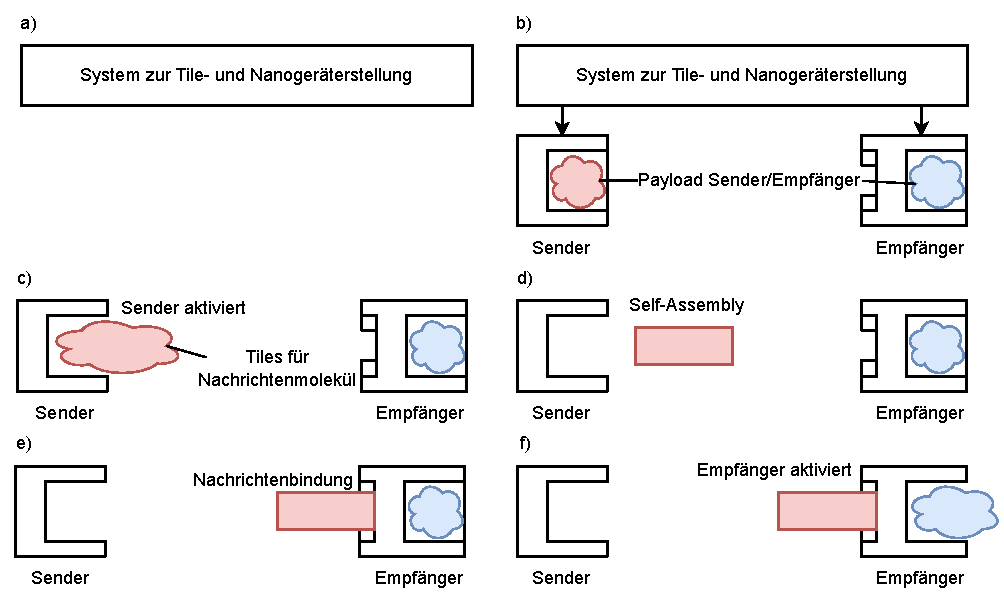
\includegraphics[width=\textwidth]{images/One-Way Communication.pdf}
    \caption[Einweg Kommunikation]{Skizzierte Darstellung einer Kommunikation von Nanogeräten, die nach dem Senden einer Nachricht aufgelöst oder aus dem System entfernt werden können. Dafür liegt in a) ein System zur Erstellung von Nanogeräten und Tiles vor. Dieses erstellt in b) den Sender und den Empfänger für den Kommunikationsschritt. Auch die Payloads beider Akteure werden durch das System gebildet. In c) werden die Tiles für die Self-Assembly durch die Aktivierung des Senders freigegeben. Diese Aktivierung kann durch unterschiedliche Mechanismen erfolgen. Das Binden von Liganden an Rezeptoren des Gerätes oder die Registrierung von Markern sind mögliche Mechanismen dafür. In d) wird das Nachrichtenmolekül durch Self-Assembly gebildet und in e) beim Empfänger gebunden. Dieser lässt daraufhin die Payload frei. Der Inhalt der Payload kann je nach Anwendungsfall unterschiedlich aussehen.}
    \label{fig:onewaycomm}
\end{figure}

\begin{figure}
    \centering
    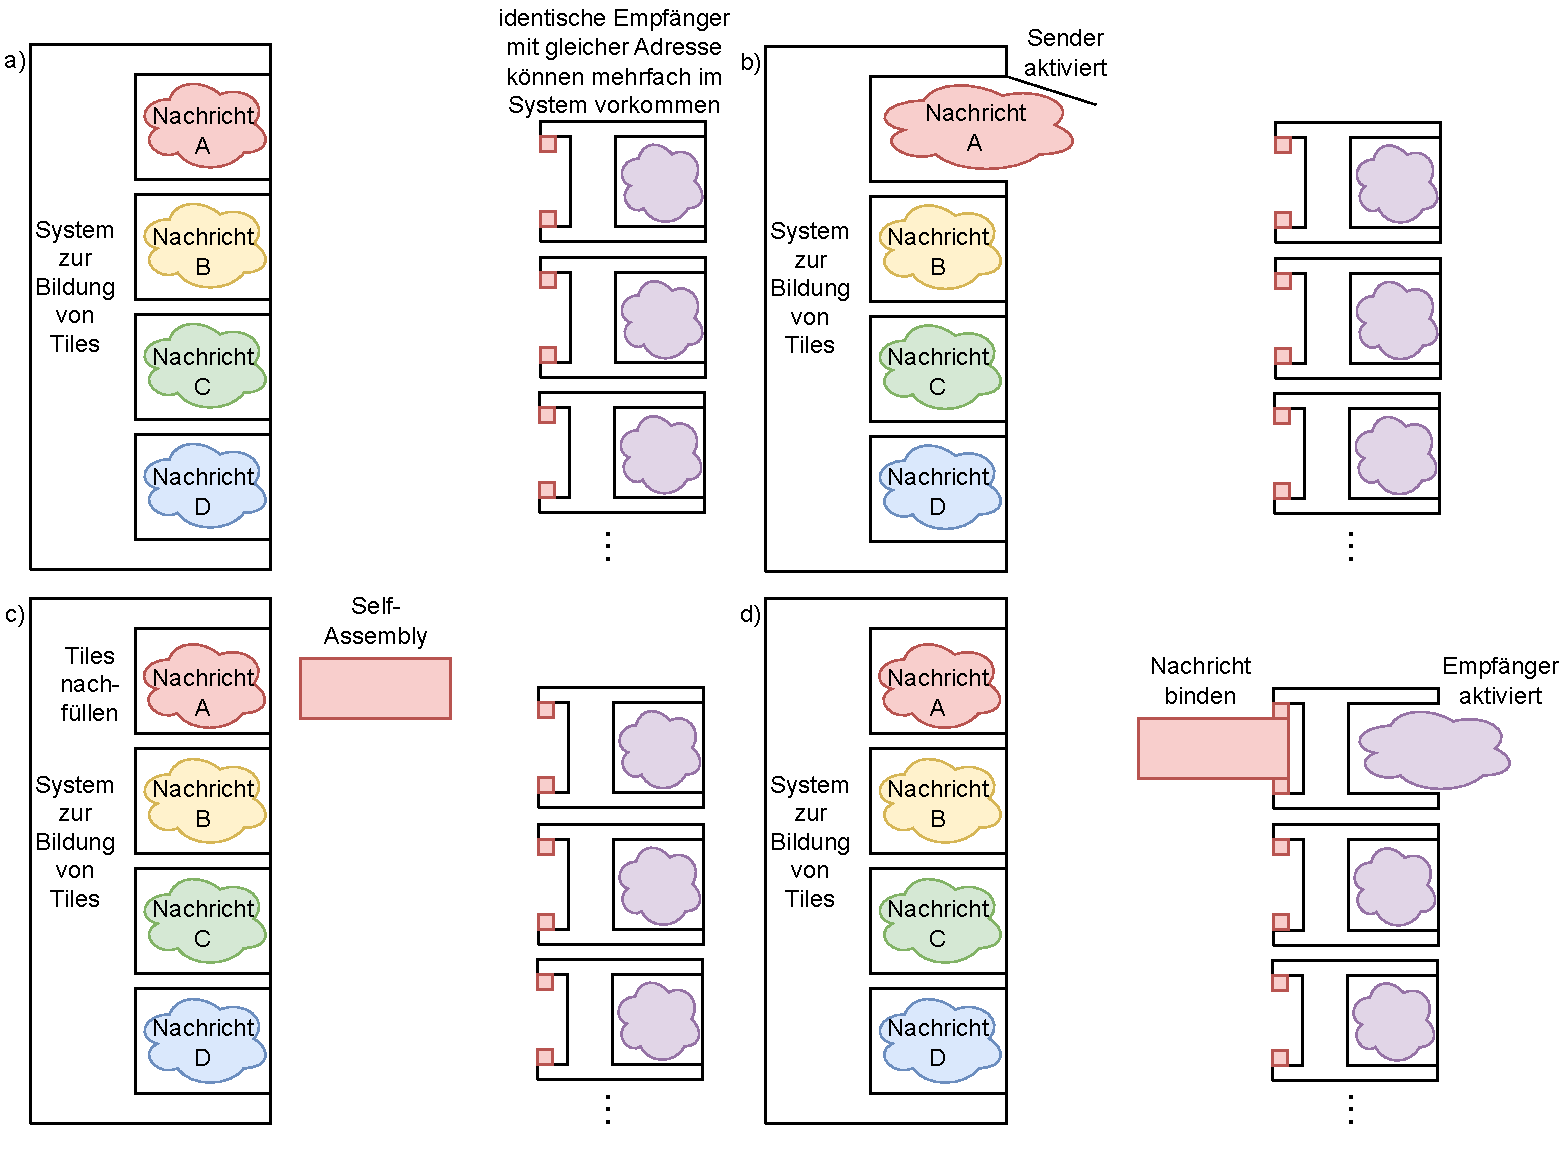
\includegraphics[width=\textwidth]{images/Multi-Way-Communication2.pdf}
    \caption[Mehrweg Kommunikation]{Skizzierte Darstellung einer Kommunikation von Nanogeräten, die erneutes Senden unterschiedlicher Nachrichten ermöglicht. In a) ist das System vorgestellt, welches das wiederholte Senden von Nachrichten ermöglicht. In b) wird das Nanogerät aktiviert, sodass eine Tileset freigelassen wird. Die Aktivierung kann durch unterschiedliche Mechanismen erfolgen. Eine Möglichkeit ist die Markererkennung oder die Bindung von Liganden an Rezeptoren. In c) kommt es zur Self-Assembly. Auch wird gezeigt, dass in so einem System die gleiche Nachricht erneut gesendet werden kann. In d) bindet sich die Nachricht beim Empfänger und dieser wird aktiviert. Damit kann beispielsweise die Payload des Empfängers freigelassen werden.}
    \label{fig:multiwaycomm}
\end{figure}

\section{Datenflusskontrolle durch Acknowledgements in Nanonetzwerken}

Der erste vorgestellte Mechanismus behandelt gleich drei der betrachteten Anforderungen an Datenflusskontrolle: die Vermeidung der Überlastung des Systems, die Effizienz und die Fehlerbehandlung.
Für Acknowledgements sind einige Faktoren interessant. Neben der Lebensdauer eines DNA-Moleküls im System $t_{deg}$ sind hier noch zwei weitere Angaben relevant. Die durchschnittliche Dauer zur Bildung eines Nachrichtenmoleküls durch Self-Assembly $t_{sa}(\tau,n)$. Diese ist abhängig von Temperatur $\tau$ des Systems und der Größe $n$ des Moleküls. Die Größe des Moleküls lässt sich dabei aus der Menge der Tiles bestimmen, die zur Konstruktion des gesamten Nachrichtenmoleküls verbunden werden. Der zweite wichtige Parameter ist die durchschnittliche Dauer des Bindens eines kompletten Moleküls nach Self-Assembly mit dem Empfänger des Nachrichtenmoleküls $t_{bind}$.

Um die Überlastung zu verringern, werden weitere Tilesets in den Prozess der Kommunikation verwendet. 
Ein Empfänger lässt beim Binden des Nachrichtenmoleküls ein solches Tileset frei. In Abbildung~\ref{fig:acks} sind zwei mögliche Self-Assemblies zu erkennen. Diese Assemblies stellen Acknowledgements dar, die schnellstmöglich gebildet und beim Sender gebunden werden, um den Erhalt der initialen Nachricht zu bestätigen. 
Dafür kann das Acknowledgement für ein möglichst kleines Molekül wie in Abbildung~\ref{fig:acks} a) nur aus einem Seed-Tile und einem Tile für die Liganden bestehen, der die Adressierung bestimmt. Eine andere Möglichkeit ist, dass es aus neun Tiles wie in Abbildung~\ref{fig:acks} b) besteht. 

Das Acknowledgement ist in diesen beiden Assemblies durch $\sigma_x$ und $K_x$ mit einen Index $x$ dargestellt. Dieser beschreibt die Notwendigkeit von eindeutigen Acknowledgements für jeden Kommunikationsvorgang. 
Es muss verhindert werden, dass ein Sender ein Acknowledgement einer vergangenen Nachricht verspätet erhält und sie für das Acknowledgement des zuletzt geschickten Nachrichtenmoleküls hält.
Das geschieht nur unter der Annahme, dass $t_{deg}$ groß genug gewählt ist. Somit können Assemblies und Tiles über mehrere Kommunikationsvorgänge nicht aus dem System entfernt werden. 
Somit benötigt jedes Acknowledgement einen eindeutigen Bezeichner, der je nach Kontext unterschiedlich festgelegt werden kann.
Die Assemblies in Abbildung~\ref{fig:acks} sind dabei nur Beispiele für Acknowledgements. In b) ist das Molekül zwar größer, jedoch kann dies je nach Anwendungsfall notwendig sein.
Ein anderer Ansatz für ein minimales Acknowledgement wie in a) könnte ein einzelnes Tile sein, welches sowohl Ligand als auch Seed-Assembly ist. 

\begin{figure}
    \centering
    \begin{tikzpicture}
        % Big ACK
        \node at (-1.2,2.3) {b)};
        \tileBigACKA{0}{1.2}
        \tileBigACKSigma{0}{0}
        \tileBigACKD{0}{-1.2}
        %
        \tileBigACKB{-1.2}{1.2}
        \tileBigACKKx{-1.2}{0}
        \tileBigACKE{-1.2}{-1.2}
        %
        \tileBigACKC{-2.4}{1.2}
        \tileBigACKM{-2.4}{0}
        \tileBigACKF{-2.4}{-1.2}
        % Small ACK
        \node at (-6.6,2.3) {a)};
        \tileSmallACKSigmax{-6}{0}
        \tileSmallACKA{-7.2}{0}
    \end{tikzpicture}
    \caption[Acknowledgements Tiles und Moleküle]{Darstellung von möglichen Acknowledgement Molekülen. In a) der Molekülhöhe eins und in b) der Molekülhöhe drei. Andere Größen und Formen für Acknowledgements sind denkbar und werden im Kapitel~\ref{cha:simulationen} näher betrachtet. Hier sind zwei Beispiele zur Veranschaulichung dargestellt.}
    \label{fig:acks}
\end{figure}

Es kann im Folgenden angenommen werden, dass ein Mechanismus im System existiert, der Acknowledgements nach dem Empfang der Nachricht freilässt. Dieses Nachrichtenmolekül kann sich dann beim Sender binden und gibt so die Bestätigung der erfolgreichen Übertragung. Auf dieser Basis kann Datenflusskontrolle durchgeführt werden.

Ein Sender lässt das Tileset für ein Nachrichtenmolekül frei. Für eine beliebige Übertragung und deren Dauer $t_{trans}$ gilt: Sei ein Nachrichtenmolekül der Größe $n$, bei einer Systemtemperatur $\tau$ und einem je nach Anwendung gewähltem Zeitpolster $t_w$ gegeben, kann folgendes betrachtet werden:
\begin{align*}
    \text{Neuübertragung}
    \begin{cases}
        \text{ja, } &\text{wenn } \lnot ACK \land t_{trans} > 2*(t_{sa}(\tau,n) + t_{bind}) + t_w\\
        \text{nein, } &\text{sonst }
    \end{cases}
\end{align*}

Dabei wird betrachtet, unter welchen Umständen es zu einer Neuübertragung kommt. Wenn innerhalb des durchschnittlichen Übertragungszeitraums zuzüglich eines Zeitpolsters kein Acknowledgement empfangen wird, erfolgt eine Neuübertragung.
Das Zeitpolster $t_w$ muss dabei so gewählt sein, dass nach Möglichkeit keine False-Positives für eine Neuübertragung entstehen. 
Dabei wird angenommen, dass das Sendermolekül größer ist als das Acknowledgement. Ist dies nicht der Fall, so muss $t_{sa}$ für das größere der beiden Moleküle betrachtet werden.

Durch diesen Mechanismus wird verhindert, dass ein langsamer Empfänger von einem schnellen Sender überlastet wird. Eine Optimierung der Zeitfenster steigert zudem die Effizienz, indem sie schnelle Neuübertragungen ermöglicht. Auch werden verlorene Nachrichten durch einen solchen Mechanismus erkannt und können durch die Neuübertragung wiederholt werden. Damit sind mit der Fehlerbehandlung drei der betrachteten Anforderungen an die Datenflusskontrolle vorgestellt. Im Folgenden soll der Aspekt der Gerechtigkeit im Medium betrachtet werden.

\section{Datenflusskontrolle durch Prioritätslevel in Nanonetzwerken}

\begin{table}
    \centering
    \begin{tabular}{l|l|l}
        & & Erlaubte Übertragung \\
        Priorität & Beispielhafter Nachrichtentyp & pro $t_{deg}$ Zyklus \\\hline 
        1 & Notfallbenachrichtigung & $\infty$ \\
        2 & Anweisung zur Medikamentausschüttung & $5$ \\
        3 & spezifische Werte anfragen & $3$ \\
        4 & allgemeiner Check & $1$
    \end{tabular}
    \caption[Prioritäten Beispiel]{Beispielhafte Einteilung von Nachrichtentypen in verschiedene Prioritätslevel für ein medizinischen System. Allen Prioritätsleveln wird aus Gerechtigkeitsgründen eine erlaubte Menge an Übertragungen pro Zyklus zugeteilt. Ein Zyklus stellt dabei die Zeitspanne $t_{deg}$ dar, welche die durchschnittliche Dauer des Verfalls oder Entfernung eines Tiles im Medium darstellt.}
    \label{tab:prio_gerechtigkeit}
\end{table}

Die Gerechtigkeit ist ein weiterer Faktor der Datenflusskontrolle. Dabei soll sichergestellt werden, dass alle Agierenden im Netzwerk regelmäßigen Zugriff auf das Medium erhalten. In einem Nanonetzwerk ist es jedoch schwierig, ohne Overhead einen Überblick darüber zu gewinnen, wer welche Nachrichten verschickt hat. Eine Lösung wäre es, durch ein zentrales Steuermedium verschiedene \emph{Prioritätslevel} für verschiedene Nachrichtentypen festzulegen. Dies ist beispielhaft in Tabelle~\ref{tab:prio_gerechtigkeit} für den Kontext In-Body-Networks dargestellt. Im Beispiel aus dieser Tabelle werden spezifischen Nachrichten eine höhere Priorität gegeben. Diese können unendlich oft oder mehrfach während eines $t_{deg}$ Zeitfensters übertragen werden. Nachrichten von niedriger Priorität jedoch nur wenige Male oder nur einmal. Durch einen solchen Mechanismus kann keine Gerechtigkeit garantiert werden, jedoch kann so verhindert werden, dass Beteiligte im Netzwerk das Medium mit \glqq unwichtigen\grqq\, Nachrichten flutet.

Dabei ist wichtig zu betonen, dass dieser Mechanismus vor allem dann von Bedeutung ist, wenn angenommen wird, dass das Medium in einem DNA-Tile-basierten Nanonetzwerk überflutet werden kann. Eine Stärke dieser Technologie ist ihre inhärente Parallelität: bei korrekt definierten Tilesets können mehrere Self-Assemblies simultan im selben Medium ablaufen, ohne Fehler zu verursachen. Dennoch könnte es Systeme geben, in denen ein Mechanismus zur Gerechtigkeit im Medium wichtig ist: beispielweise bei einer zentralen Steuerung, die durch eine Vielzahl von Nachrichten überlastet werden könnte. Daher kann ein Gerechtigkeitsmechanismus im Medium in bestimmten Anwendungsfällen durchaus sinnvoll sein.

Da einige Aspekte der Datenflusskontrolle mit Acknowledgements und Prioritätsleveln abgedeckt sind, kann mit der nächsten Anforderung weiter gemacht werden. 

\section{Nachrichtencodierung in Nanonetzwerken}
\label{sec:message_code}

Die nächste betrachtete Anforderung lässt sich schwer auf einzelne Anforderungen aus Kommunikationsprotokollen abbilden. Dabei geht es um die Darstellung von Nachrichten auf der Nanoebene. So wie in anderen Systemen müssen bei der Kommunikation in Nanonetzwerken Nachrichten zwischen Geräten verschickt werden. Diese werden durch Self-Assembly gebildet und durch die Bindung zwischen Liganden und Rezeptoren empfangen. Dabei muss das Nanogerät, das die Nachricht bindet, eine beliebige Nachricht $x$ von einer anderen Nachricht $y$ unterscheiden können.

Dafür soll in dieser Sektion eine Möglichkeit geliefert werden, mit welcher eine beliebige Anzahl an Nachrichten in einem System durch Tilesets und deren Self-Assembly gebildet werden können. Dabei liegt der Fokus darauf, die Nachrichtenmoleküle möglichst klein zu halten, ohne dabei zu große Tilesets zu erstellen. Die genaue Gewichtung dieser beiden Faktoren wird in Kapitel~\ref{cha:konstruktion} diskutiert.

Zur Codierung von Nachrichten auf Nanonetzwerkebene werden zwei Möglichkeiten vorgestellt: die Kodierung in den Kleberbezeichnern und die Kodierung in den Tilebezeichnern.
Wie beim Thema der Adressierung beschrieben wurde, können offene DNA-Stränge zur Informationskodierung verwendet werden. Somit ist auch die Informationskodierung in Kleberbezeichnern möglich.
Wenn die Information nicht in den Kleberbezeichnern codiert wird, kann sie auch in den Tilebezeichnern codiert werden. 

Dabei spielt die Struktur der gebildeten Tiles die entscheidende Rolle für die Codierung, nicht die offenen DNA-Enden.
Beispiele für beide Codierungsarten sind in Abbildung~\ref{fig:kodierung_glues} und Abbildung~\ref{fig:kodierung_label} gegeben. Beide Beispiele zeigen im Beispiel b) eine Self-Assembly für die Hexadezimalzahl \texttt{ab1}. In Abbildung~\ref{fig:kodierung_glues} sind in a) alle Tiles zu sehen, die zur Codierung von dreistelligen Hexadezimalzahlen in den Kleberbezeichnern benötigt werden. Insgesamt 100 Tiles sind notwendig und die finale Self-Assembly besteht aus zehn Tiles. Es ist möglich zwei Tiles im Tileset und der Self-Assembly zu sparen, indem die Liganden mit den Bezeichnern \glqq Z\grqq\, und \glqq K\grqq\, entfernt werden. Dann müssten alle Tiles mit den Bezeichnern \glqq Y\grqq\, und \glqq J\grqq\ die Liganden bilden. Somit würde das Tileset 98 Tiles umfassen und die Self-Assembly acht Tiles. Aus Gründen der Übersichtlichkeit wurde dies im Beispiel aus Abbildung~\ref{fig:kodierung_glues} nicht getan. Das Prinzip wird jedoch im Beispiel aus Abbildung~\ref{fig:kodierung_label} angewendet. Auch hier sind in a) alle Tiles dargestellt, die zur Codierung einer dreistelligen Hexadezimalzahl benötigt werden. In b) ist die beispielhafte Self-Assembly zu sehen. Dieser Ansatz benötigt 48 Tiles im Tileset und vier Tiles in der Self-Assembly. Wird angenommen, dass auch hier die Liganden in einzelnen Tiles gebildet werden, verändert sich das leicht. Dabei wäre das Tileset 49 Tiles und die Assembly fünf Tiles groß.

\begin{figure}
    \centering
    \begin{tikzpicture}[scale = 0.9]
        % Sigma/V/K/Z-Tile
        \node at (-1,-7.5) {a)};
        \tileCodeGluesSigma{0}{0}
        \tileCodeGluesV{1.5}{0}
        \tileCodeGluesK{3}{0}
        \tileCodeGluesZ{4.5}{0}
        % Row 1
        \tileCodeGluesWNull{0}{-1.5}
        \tileCodeGluesWEins{1.5}{-1.5}
        \tileCodeGluesWZwei{3}{-1.5}
        \tileCodeGluesWDrei{4.5}{-1.5}
        \tileCodeGluesWVier{6}{-1.5}
        \tileCodeGluesWFuenf{7.5}{-1.5}
        \tileCodeGluesWSechs{9}{-1.5}
        \tileCodeGluesWSieben{10.5}{-1.5}
        \tileCodeGluesWAcht{12}{-1.5}
        \tileCodeGluesWNeun{13.5}{-1.5}
        % Row 2
        \tileCodeGluesWA{0}{-3}
        \tileCodeGluesWB{1.5}{-3}
        \tileCodeGluesWC{3}{-3}
        \tileCodeGluesWD{4.5}{-3}
        \tileCodeGluesWE{6}{-3}
        \tileCodeGluesWD{7.5}{-3}
        \tileCodeGluesXNull{9}{-3}
        \tileCodeGluesXEins{10.5}{-3}
        \tileCodeGluesXZwei{12}{-3}
        \tileCodeGluesXDrei{13.5}{-3}
        % Row 3
        \tileCodeGluesXVier{0}{-4.5}
        \tileCodeGluesXFuenf{1.5}{-4.5}
        \tileCodeGluesXSechs{3}{-4.5}
        \tileCodeGluesXSieben{4.5}{-4.5}
        \tileCodeGluesXAcht{6}{-4.5}
        \tileCodeGluesXNeun{7.5}{-4.5}
        \tileCodeGluesXA{9}{-4.5}
        \tileCodeGluesXB{10.5}{-4.5}
        \tileCodeGluesXC{12}{-4.5}
        \tileCodeGluesXD{13.5}{-4.5}
        % Row 4
        \tileCodeGluesXE{0}{-6}
        \tileCodeGluesXF{1.5}{-6}
        \tileCodeGluesYNull{3}{-6}
        \tileCodeGluesYEins{4.5}{-6}
        \tileCodeGluesYZwei{6}{-6}
        \tileCodeGluesYDrei{7.5}{-6}
        \tileCodeGluesYVier{9}{-6}
        \tileCodeGluesYFuenf{10.5}{-6}
        \tileCodeGluesYSechs{12}{-6}
        \tileCodeGluesYSieben{13.5}{-6}
        % Row 5
        \tileCodeGluesYAcht{0}{-7.5}
        \tileCodeGluesYNeun{1.5}{-7.5}
        \tileCodeGluesYA{3}{-7.5}
        \tileCodeGluesYB{4.5}{-7.5}
        \tileCodeGluesYC{6}{-7.5}
        \tileCodeGluesYD{7.5}{-7.5}
        \tileCodeGluesYE{9}{-7.5}
        \tileCodeGluesYF{10.5}{-7.5}
        \tileCodeGluesHNull{12}{-7.5}
        \tileCodeGluesHEins{13.5}{-7.5}
        % Row 6
        \tileCodeGluesHZwei{0}{-9}
        \tileCodeGluesHDrei{1.5}{-9}
        \tileCodeGluesHVier{3}{-9}
        \tileCodeGluesHFuenf{4.5}{-9}
        \tileCodeGluesHSechs{6}{-9}
        \tileCodeGluesHSieben{7.5}{-9}
        \tileCodeGluesHSieben{9}{-9}
        \tileCodeGluesHAcht{10.5}{-9}
        \tileCodeGluesHNeun{12}{-9}
        \tileCodeGluesHA{13.5}{-9}
        % Row 7
        \tileCodeGluesHB{0}{-10.5}
        \tileCodeGluesHC{1.5}{-10.5}
        \tileCodeGluesHD{3}{-10.5}
        \tileCodeGluesHE{4.5}{-10.5}
        \tileCodeGluesHF{6}{-10.5}
        \tileCodeGluesINull{7.5}{-10.5}
        \tileCodeGluesIEins{9}{-10.5}
        \tileCodeGluesIZwei{10.5}{-10.5}
        \tileCodeGluesIDrei{12}{-10.5}
        \tileCodeGluesIVier{13.5}{-10.5}
        % H-Tiles Row 2
        \tileCodeGluesIFuenf{0}{-12}
        \tileCodeGluesISechs{1.5}{-12}
        \tileCodeGluesISieben{3}{-12}
        \tileCodeGluesIAcht{4.5}{-12}
        \tileCodeGluesINeun{6}{-12}
        \tileCodeGluesIA{7.5}{-12}
        \tileCodeGluesIB{9}{-12}
        \tileCodeGluesIC{10.5}{-12}
        \tileCodeGluesID{12}{-12}
        \tileCodeGluesIE{13.5}{-12}
        % Row 8
        \tileCodeGluesIF{0}{-13.5}
        \tileCodeGluesJNull{1.5}{-13.5}
        \tileCodeGluesJEins{3}{-13.5}
        \tileCodeGluesJZwei{4.5}{-13.5}
        \tileCodeGluesJDrei{6}{-13.5}
        \tileCodeGluesJVier{7.5}{-13.5}
        \tileCodeGluesJFuenf{9}{-13.5}
        \tileCodeGluesJSechs{10.5}{-13.5}
        \tileCodeGluesJSieben{12}{-13.5}
        \tileCodeGluesJAcht{13.5}{-13.5}
        % Row 9
        \tileCodeGluesJA{0}{-15}
        \tileCodeGluesJB{1.5}{-15}
        \tileCodeGluesJC{3}{-15}
        \tileCodeGluesJD{4.5}{-15}
        \tileCodeGluesJE{6}{-15}
        \tileCodeGluesJF{7.5}{-15}
        %%%% 
        % Bsp. Assembly Row 1
        \draw[line width=1pt] (-0.6,-16) -- (14.1,-16);
        \node at (-1,-17.8) {b)};
        \tileCodeGluesZ{0}{-17.2}
        \tileCodeGluesYA{1.2}{-17.2}
        \tileCodeGluesXB{2.4}{-17.2}
        \tileCodeGluesWEins{3.6}{-17.2}
        \tileCodeGluesV{4.8}{-17.2}
        % Bsp. Assembly Row 2
        \tileCodeGluesK{0}{-18.4}
        \tileCodeGluesJA{1.2}{-18.4}
        \tileCodeGluesIB{2.4}{-18.4}
        \tileCodeGluesHEins{3.6}{-18.4}
        \tileCodeGluesSigma{4.8}{-18.4}
        \draw[line width=1.5pt, green] (0.9,-18.2) rectangle (3.9,-17.4);
    \end{tikzpicture}
    \caption[Dreistellige Hexadezimalzahl in den Kleberbezeichnern codiert]{Beispielhafte Codierung der dreistelligen Hexadezimalzahl \texttt{ab1} (grün), wobei die Codierung in den Kleberbezeichnern stattfindet. In a) ist dafür das Tileset für alle notwendigen Tiles zur Codierung einer dreistelligen Hexadezimalzahl in den Kleberbezeichnern abgebildet. In b) ist die Self-Assembly für die Hexadezimalzahl \texttt{ab1} abgebildet.}
    \label{fig:kodierung_glues}
\end{figure}

Wird bei beiden Ansätzen davon ausgegangen, dass sie den Beispielen aus den Abbildungen \ref{fig:kodierung_glues} und \ref{fig:kodierung_label} folgen, dann lässt sich für eine Zahl im Basis-$x$-System und der Anzahl der Ziffern $y$ Folgendes sagen:
Wird die Zahl in den Kleberbezeichnern codiert, so hat das Tileset $2xy + 4$ Tiles und die Self-Assembly $2y+4$ Tiles.
Wird die Zahl in einem einzelnen Tile codiert, dann hat das Tileset $yx+1$ Tiles und die Self-Assembly $y+1$ Tiles.
In den Beispielen aus Abbildungen \ref{fig:kodierung_glues} und \ref{fig:kodierung_label} liegt eine Hexadezimalzahl mit drei Ziffernstellen vor. Somit lässt sich beispielsweise für Kleberbezeichner $2\cdot 16\cdot 3+4 = 100$ berechnen.
Für sowohl die Größe der Self-Assembly als auch für die Größe des benötigten Tilesets kann erkannt werden, dass die Codierung in den Bezeichnern des Tiles effizienter ist, da jede Ziffer eines beliebigen Zahlensystems durch ein statt zwei Tiles dargestellt werden kann.

Jedoch muss dabei betrachtet werden, dass die Tilebezeichner auf der mathematischen Ebene verwendet werden, damit Nutzer*innen des Systems eine bessere Übersicht über die verschiedenen Tiles haben. 
Um darin die Codierung durchzuführen, muss ein neuer Ansatz gefunden werden, der diese Bezeichner auch im praktischen Anwendungsfall ermöglicht. 
Ein Vorschlag dafür ist die interne Struktur des Tiles zu verwenden, um Bezeichner zu realisieren. 
Die DNA-Basenpaare im Inneren des Tiles können so analysiert und spezifisch für einen Bezeichner verwendet werden.

\begin{figure}
    \centering
    \begin{tikzpicture}[scale=0.9]
        % Sigma-Tile
        \node at (-1,-3.75) {a)};
        \tileCodeLabelSigma{0}{0}
        % X-Tiles Row 1
        \tileCodeLabelXNull{0}{-1.5}
        \tileCodeLabelXEins{1.5}{-1.5}
        \tileCodeLabelXZwei{3}{-1.5}
        \tileCodeLabelXDrei{4.5}{-1.5}
        \tileCodeLabelXVier{6}{-1.5}
        \tileCodeLabelXFuenf{7.5}{-1.5}
        \tileCodeLabelXSechs{9}{-1.5}
        \tileCodeLabelXSieben{10.5}{-1.5}
        \tileCodeLabelXAcht{12}{-1.5}
        \tileCodeLabelXNeun{13.5}{-1.5}
        % X-Tiles Row 2
        \tileCodeLabelXA{0}{-3}
        \tileCodeLabelXB{1.5}{-3}
        \tileCodeLabelXC{3}{-3}
        \tileCodeLabelXD{4.5}{-3}
        \tileCodeLabelXE{6}{-3}
        \tileCodeLabelXF{7.5}{-3}
        \tileCodeLabelYNull{9}{-3}
        \tileCodeLabelYEins{10.5}{-3}
        \tileCodeLabelYZwei{12}{-3}
        \tileCodeLabelYDrei{13.5}{-3}
        % Y-Tiles Row 1
        \tileCodeLabelYVier{0}{-4.5}
        \tileCodeLabelYFuenf{1.5}{-4.5}
        \tileCodeLabelYSechs{3}{-4.5}
        \tileCodeLabelYSieben{4.5}{-4.5}
        \tileCodeLabelYAcht{6}{-4.5}
        \tileCodeLabelYNeun{7.5}{-4.5}
        \tileCodeLabelYA{9}{-4.5}
        \tileCodeLabelYB{10.5}{-4.5}
        \tileCodeLabelYC{12}{-4.5}
        \tileCodeLabelYD{13.5}{-4.5}
        % Y-Tiles Row 2
        \tileCodeLabelYE{0}{-6}
        \tileCodeLabelYF{1.5}{-6}
        \tileCodeLabelZEins{3}{-6}
        \tileCodeLabelZZwei{4.5}{-6}
        \tileCodeLabelZDrei{6}{-6}
        \tileCodeLabelZVier{7.5}{-6}
        \tileCodeLabelZFuenf{9}{-6}
        \tileCodeLabelZSechs{10.5}{-6}
        \tileCodeLabelZSieben{12}{-6}
        \tileCodeLabelZAcht{13.5}{-6}
        % Z-Tiles Row 1
        \tileCodeLabelZNeun{0}{-7.5}
        \tileCodeLabelZA{1.5}{-7.5}
        \tileCodeLabelZB{3}{-7.5}
        \tileCodeLabelZC{4.5}{-7.5}
        \tileCodeLabelZD{6}{-7.5}
        \tileCodeLabelZE{7.5}{-7.5}
        \tileCodeLabelZF{9}{-7.5}
        %%%% 
        % Bsp. Assembly Row 1
        \draw[line width=1pt] (-0.6,-8.5) -- (14.1,-8.5);
        \node at (-1,-9.5) {b)};
        \tileCodeLabelZA{0}{-9.5}
        \tileCodeLabelYB{1.2}{-9.5}
        \tileCodeLabelXEins{2.4}{-9.5}
        \tileCodeLabelSigma{3.6}{-9.5}
        \draw[line width=1.5pt, green] (-0.3,-9.3) rectangle (2.6,-9.7);
    \end{tikzpicture}
    \caption[Dreistellige Hexadezimalzahl in den Tile Bezeichnern codiert]{Beispielhafte Codierung der dreistelligen Hexadezimalzahl \texttt{ab1} (grün), wobei die Codierung in den Tilebezeichnern stattfindet. In a) ist dafür das Tileset für alle notwendigen Tiles zur Codierung einer dreistelligen Hexadezimalzahl in den Tilebezeichnern abgebildet. In b) ist die Self-Assembly für die Hexadezimalzahl \texttt{ab1} abgebildet.}
    \label{fig:kodierung_label}
\end{figure}

Wenn in einem Nanonetzwerk eine beliebige Anzahl unterschiedlicher Nachrichten vorhanden ist, können diese in ein entsprechendes Zahlensystem übertragen werden. Als Beispiel dient dabei wieder das In-Body-Network. Gibt es im Netzwerk beispielsweise 20 unterschiedliche Kontrollnachrichten und 200 verschiedene Krankheitsbilder, die durch Nachrichten übermittelt werden sollen, so ergibt das insgesamt 220 Nachrichten. Mit einer zweistelligen Hexadezimalzahl könnten 256 Nachrichten codiert werden, wofür 33 Tiles für das Tileset und drei Tiles für die Self-Assembly benötigt werden.

Sollte das Netzwerk jedoch 300 verschiedene Krankheitsbilder unterstützen, wäre eine zweistellige Hexadezimalzahl unzulänglich.
Obwohl eine dreistellige Hexadezimalzahl die Kapazität hat, ist es ineffizient, eine Zahl zu wählen, die 4096 Nachrichten kodieren kann. Dabei werden 49 Tiles im Tileset und vier Tiles in der Self-Assembly benötigt. Da nur 320 Nachrichten kodiert werden müssen, sollte ein kleineres Zahlensystem gewählt werden. Ein effizienterer Ansatz wäre die Verwendung einer dreistelligen Oktalzahl. Hierbei würden 25 Tiles für das Tileset und vier Tiles für die Self-Assembly ausreichen, um 320 Nachrichten zu kodieren.

Die Entscheidung für das optimale Zahlensystem hängt von der Gewichtung zwischen der Größe der Self-Assembly und der Größe des Tilesets ab. Wird die Tilebezeichner-Codierung verwendet, sollte das Zahlensystem so gewählt werden, dass die Ergebnisse der Formeln $xy+1$ und $y+1$ (für $y$-stellige Zahl der Basis $x$) möglichst gering sind. Werden diesen Formeln spezifische Gewichtungen zugewiesen, kann das Auswahlverfahren durch den folgenden Pseudocode repräsentiert werden:


\begin{lstlisting}[language=Python, caption={[Pseudocode für eine Funktion zur Definition der besten Basis.]{Pseudocode für eine Funktion zur Definition der besten Basis abhängig von der Anzahl der zu codierenden Nachrichten und den Gewichtungen von Tileset und Assembly. Der gesamte Code ist im Anhang \ref{app:code} verlinkt.}}, label=lst:best_base]
# m = Anzahl der Nachrichten die codiert werden muss
# w1 = Gewichtung Formel 1 (xy+1)
# w2 = Gewichtung Formel 2 (y+1)
def get_best_base(m, w1, w2):
    # initialisieren
    best_base = 2
    best_score = inf 
    best_f1 = 0
    best_f2 = 0

    for b in range(2, m+1)
        # bestimme Anzahl der Ziffern von m zur Basis b
        y = convert_m_to_base(m, b)
        f1 = b * y + 1
        f2 = y + 1
        score = w1 * f1 * w2 * f2
        # wenn der aktuelle Score kleiner ist, 
        # liegt effizientere Basis vor
        if score < best_score
            best_score = score 
            best_base = base 
            best_f1 = f1 
            best_f2 = f2
    return best_base, best_f1, best_f2
\end{lstlisting}

Die Gewichtung der Formeln kann beliebig gewählt werden. Ist die Gewichtung beispielsweise $w_1 = 1$ und $w_2 = 10$, so bedeutet dies, dass ein Tile in der Self-Assembly das gleiche Gewicht hat wie zehn Tiles im Tileset.

In dieser Sektion wurde für Erklärungszwecke vereinfacht angenommen, dass die Codierung von DNA-Tiles auf verschiedene Zahlensysteme trivial ist. Tatsächlich erfolgt die Codierung auf Nanoebene stets in der DNA-Sprache von \emph{ATCG}. Dafür wird angenommen, dass DNA analog auf Binärzahlen übertragen werden kann. So kann jedes \emph{AT} oder \emph{TA} Basenpaar beispielsweise binär als \texttt{0} und jedes Basenpaar \emph{CG} oder \emph{GC} binär als \texttt{1} codiert werden. Auch ein ein Zahlensystem der Basis vier ist denkbar, das die Reihenfolge der Basenpaare berücksichtigt.

Die Umwandlung von Binärzahlen in andere Zahlensysteme, wie Hexadezimalzahlen, kann ohne Overhead erfolgen. Beispielsweise lässt sich eine vierstellige Binärzahl direkt in eine Hexadezimalzahl übersetzen. Komplikationen ergeben sich jedoch, wenn man Binärzahlen in ein Dezimalsystem umwandeln möchte. Während eine vierstellige Binärzahl 16 Zahlen darstellen kann, ist eine dreistellige Binärzahl auf acht Zahlen beschränkt. Dies kann zu Overhead in der Codierung führen.

Da in dieser Arbeit das mathematische Tile-Modell betrachtet wird und die Codierung in den mathematischen Bezeichnern stattfindet, wird dies in der Arbeit nicht weiter betrachtet. Sollte der Mechanismus in einem Nanonetzwerk implementiert werden, muss darauf geachtet werden.  

Nach Auswahl des effizientesten Zahlensystems können Nachrichten mittels Preprocessing in das entsprechende System umgewandelt werden. Dies ermöglicht die Erstellung von Nachrichtenmolekülen mit minimaler Anzahl an Tiles und kleinstmöglichen Assemblies für das Netzwerk. Weiterhin ermöglicht das Preprocessing eine Optimierung der benötigten Nachrichtenanzahl. Einige Nachrichten könnten eventuell durch den Einsatz von Flags optimiert werden, die in der Sektion~\ref{sec:flags} näher erläutert werden.

\section{Self-Assemblies in ihrer Höhe anpassen}

Bevor mit weiteren Anforderungen fortgefahren wird, muss zunächst die Höhe von Self-Assemblies thematisiert werden. In dieser Arbeit werden verschiedene Self-Assemblies dargestellt, die unterschiedliche Höhen aufweisen. Eine Verringerung der Höhe einer Self-Assembly ist nicht immer möglich, da hierbei Informationen verloren gehen könnten. Das bislang verwendete Beispiel für den Äquivalenzvergleich aus Abbildung~\ref{fig:eq_bsp} kann beispielsweise nicht in eine Self-Assembly der Höhe zwei oder eins umgewandelt werden, ohne grundlegende Änderungen an der Struktur und Funktionsweise der Self-Assembly vorzunehmen.

Es ist jedoch trivial, die Höhe einer Self-Assembly zu erhöhen. Dies wird beispielhaft in Abbildung~\ref{fig:assembly_height} an einer Self-Assembly der Höhe eins gezeigt. Dabei müssen lediglich die Seed-Assembly und die Liganden angepasst werden. Der im Beispiel gezeigte Ligand wird zu einem Tile umfunktioniert, der die neu hinzugefügten Liganden bindet. Daher kann einer Self-Assembly der Höhe eins einfach ein Rahmen hinzugefügt werden, um ihre Höhe auf zwei oder drei zu erhöhen, ohne die eigentliche Information der Self-Assembly zu verändern.

\begin{figure}
    \centering 
    \begin{tikzpicture}
        \tileAssemblyHeightB{0}{0}
        \tileAssemblyHeightA{1.2}{0}
        \tileAssemblyHeightSigma{2.4}{0}
        %
        \node at (3.4,0) {$\Rightarrow$};
        %
        \tileAssemblyHeightBSmall{4.4}{0}
        \tileAssemblyHeightA{5.6}{0}
        \tileAssemblyHeightSigmaSmall{6.8}{0}
        %
        \tileAssemblyHeightZ{4.4}{-1.2}
        \tileAssemblyHeightY{5.6}{-1.2}
        \tileAssemblyHeightX{6.8}{-1.2}
        %
        \node at (7.8,0) {$\Rightarrow$};
        %
        \tileAssemblyHeightO{8.8}{1.2}
        \tileAssemblyHeightN{10}{1.2}
        \tileAssemblyHeightM{11.2}{1.2}
        %
        \tileAssemblyHeightBBig{8.8}{0}
        \tileAssemblyHeightA{10}{0}
        \tileAssemblyHeightSigmaBig{11.2}{0}
        %
        \tileAssemblyHeightZ{8.8}{-1.2}
        \tileAssemblyHeightY{10}{-1.2}
        \tileAssemblyHeightX{11.2}{-1.2}
        %\draw[line width=1pt] (-0.6,-3) -- (11,-3);
    \end{tikzpicture}
    \caption[Beispiel zur Vergrößerung einer Assembly]{Beispiel für das Anpassen der Höhe einer Assembly. Links ist dabei eine Self-Assembly der Höhe eins dargestellt. Diese kann durch Anpassung der Seed-Assembly und des Liganden zu einer Assembly der Höhe zwei (mittig) oder der Höhe drei (rechts) erweitert werden. Dabei verändert sich die Information der Self-Assembly selbst nicht. Nur die inneren Kleber beziehungsweise die Liganden verändern sich.}
    \label{fig:assembly_height}
\end{figure}

Dafür muss nur entweder der südliche oder nördliche Kleber von Seed-Assembly und Liganden angepasst werden. Dieser Mechanismus lässt sich für beliebige Höhen wiederholen. Dabei wird dann nicht die Seed-Assembly angepasst, sondern die Tiles nördlich und südlich der Seed-Assembly.

Mit dem beschriebenen Ansatz ist es möglich, für alle Self-Assemblies in einem System eine einheitliche Größe festzulegen. Dabei wird jedoch nicht betrachtet, ob der hinzugefügte Rahmen Informationen speichern kann, um die Effizienz der erweiterten Self-Assembly zu steigern. Dies muss individuell für jeden Fall betrachtet und neu implementiert werden. Mit diesem Verständnis über die Höhe von Self-Assemblies können nun die weiteren Anforderungen besprochen werden.

\section{Flags in Nanonetzwerken}
\label{sec:flags}
Flags werden in herkömmlichen Kommunikationsprotokollen verwendet, um bestimmte Eigenschaften oder Zustände einer Nachricht im Header zu kennzeichnen. Typische Flags sind beispielsweise Synchronisationsflags, welche in TCP verwendet werden, um einen Three-Way-Handshake zu signalisieren. Auch Acknowledgements werden in Flags verwendet, um zu signalisieren, dass das letzte Paket beim Empfänger angekommen ist. Die Finish-Flag zeigt an, dass es sich um die letzte Nachricht der Übertragung handelt, während die Reset-Flag zur abrupten Beendung einer Übertragung genutzt wird. 

Es können je nach Anwendungsfall verschiedene Flags verwendet werden. Die hier vorgestellten Flags lassen sich jedoch nicht sinnvoll auf Nanonetzwerkebene abstrahieren. Acknowledgements wurden im letzten Absatz beschrieben und können in einem offenen System als eigene Nachricht verschickt werden. In einem auf DNA und Self-Assembly basierten Nanonetzwerk, in welchem über Nachrichtenmolekülen zwischen zwei Entitäten kommuniziert wird und mehrere Nachrichten in einer Übertragung verschickt werden, könnten sich Acknowledgement-Flags anbieten. Davon wird in dieser Arbeit jedoch nicht ausgegangen. 

Synchronisation ist in Nanonetzwerken ein weiteres Problem. Dadurch, dass bei der Self-Assembly der Vorgang der Nachrichtenübertragung aus der Hand des Nutzers gegeben wird und sich alles auf dem sehr kleinen Skalenbereich der Nanoebene bewegt, lässt sich Zeit schwer synchronisieren. Es bietet sich allgemein an, asynchron zu kommunizieren. Ein Three-Way-Handshake oder andere Mechanismen, die eine relative Synchronisation zueinander ermöglichen, könnten eine Möglichkeit auf Nanoebene bieten. Dabei wird nicht die Zeit der Geräte synchronisiert, sondern ein relativer Zähler oder ein anderer Mechanismus verwendet, damit die kommunizierenden Geräte eine gemeinsam festgelegte Möglichkeit haben, um festzustellen, ob eine Nachricht verloren gegangen ist. Jedoch wurde in diesem Kapitel beschrieben, dass in Nanonetzwerken die Nachrichtenmenge minimalisiert werden soll und der Dialog von zwei Geräten über mehrere Nachrichten ungewöhnlich für Systeme auf dieser Skala ist. Somit wird für diese Arbeit asynchrone Kommunikation angenommen, da viele der Mechanismen außerhalb der Tile-basierten Self-Assembly durchgeführt werden müssten.
\begin{figure}
    \centering 
    \begin{tikzpicture}
        % Tileset Bsp 1
        \node at (-1,0) {a)};
        \tileFlagsHeigthOneC{0}{0}
        \tileFlagsHeigthOneD{1.5}{0}
        \tileFlagsHeigthOneE{3}{0}
        \tileFlagsHeigthOneSigmaAlt{4.5}{0}
        \tileFlagsHeigthOneFOne{7}{0}
        \tileFlagsHeigthOneFZero{8.5}{0}
        \tileFlagsHeigthOneSigma{10}{0}
        % Assembly Bsp 1
        \draw[line width=1pt] (-0.6,-1) -- (11,-1);
        \node at (-1,-2) {b)};
        \tileFlagsHeigthOneE{0}{-2}
        \tileFlagsHeigthOneD{1.2}{-2}
        \tileFlagsHeigthOneC{2.4}{-2}
        \tileFlagsHeigthOneSigmaAlt{3.6}{-2}
        \node at (4.6,-2) {$\Rightarrow$};
        \tileFlagsHeigthOneE{5.6}{-2}
        \tileFlagsHeigthOneD{6.8}{-2}
        \tileFlagsHeigthOneC{8}{-2}
        \tileFlagsHeigthOneFOne{9.2}{-2}
        \tileFlagsHeigthOneSigma{10.4}{-2}
        % Tileset Bsp 2
        \draw[line width=1pt] (-0.6,-3) -- (11,-3);
        \node at (-1,-5.5) {c)};
        \tileFlagsHeigthThreeSigma{0}{-4}
        \tileFlagsHeigthThreeC{1.5}{-4}
        \tileFlagsHeigthThreeD{3}{-4}
        \tileFlagsHeigthThreeE{4.5}{-4}
        %
        \tileFlagsHeigthThreeWAlt{0}{-5.5}
        \tileFlagsHeigthThreeX{1.5}{-5.5}
        \tileFlagsHeigthThreeY{3}{-5.5}
        \tileFlagsHeigthThreeZ{4.5}{-5.5}
        %
        \tileFlagsHeigthThreeMAlt{0}{-7}
        \tileFlagsHeigthThreeN{1.5}{-7}
        \tileFlagsHeigthThreeO{3}{-7}
        \tileFlagsHeigthThreeP{4.5}{-7}
        %%%%%%%%%
        \tileFlagsHeigthThreeFOne{7}{-4}
        \tileFlagsHeigthThreeFZero{8.5}{-4}
        %
        \tileFlagsHeigthThreeG{7}{-5.5}
        \tileFlagsHeigthThreeH{8.5}{-5.5}
        %
        \tileFlagsHeigthThreeW{7}{-7}
        \tileFlagsHeigthThreeM{8.5}{-7}
        % Assembly Bsp 2
        \draw[line width=1pt] (-0.6,-8) -- (11,-8);
        \node at (-1,-10.2) {d)};
        \tileFlagsHeigthThreeZ{0}{-9}
        \tileFlagsHeigthThreeE{0}{-10.2}
        \tileFlagsHeigthThreeP{0}{-11.4}
        %
        \tileFlagsHeigthThreeY{1.2}{-9}
        \tileFlagsHeigthThreeD{1.2}{-10.2}
        \tileFlagsHeigthThreeO{1.2}{-11.4}
        %
        \tileFlagsHeigthThreeX{2.4}{-9}
        \tileFlagsHeigthThreeC{2.4}{-10.2}
        \tileFlagsHeigthThreeN{2.4}{-11.4}
        %
        \tileFlagsHeigthThreeWAlt{3.6}{-9}
        \tileFlagsHeigthThreeSigma{3.6}{-10.2}
        \tileFlagsHeigthThreeMAlt{3.6}{-11.4}
        %
        \node at (4.6,-10.2) {$\Rightarrow$};
        %
        \tileFlagsHeigthThreeZ{5.6}{-9}
        \tileFlagsHeigthThreeE{5.6}{-10.2}
        \tileFlagsHeigthThreeP{5.6}{-11.4}
        %
        \tileFlagsHeigthThreeY{6.8}{-9}
        \tileFlagsHeigthThreeD{6.8}{-10.2}
        \tileFlagsHeigthThreeO{6.8}{-11.4}
        %
        \tileFlagsHeigthThreeX{8}{-9}
        \tileFlagsHeigthThreeC{8}{-10.2}
        \tileFlagsHeigthThreeN{8}{-11.4}
        %
        \tileFlagsHeigthThreeG{9.2}{-9}
        \tileFlagsHeigthThreeFOne{9.2}{-10.2}
        \tileFlagsHeigthThreeH{9.2}{-11.4}
        %
        \tileFlagsHeigthThreeW{10.4}{-9}
        \tileFlagsHeigthThreeSigma{10.4}{-10.2}
        \tileFlagsHeigthThreeM{10.4}{-11.4}
    \end{tikzpicture}
    \caption[Flags Beispiel]{Darstellung der Erweiterung von Self-Assembly Molekülen durch Flagtiles. In a) und c) sind die jeweiligen Tilesets links dargestellt. Rechts sind jeweils die Tiles dargestellt, die entweder überarbeitet (bei gleichem Bezeichner) oder neu hinzugefügt werden müssen, um Flags zu implementieren. In b) und d) sind jeweils die Umwandlungen der originalen Self-Assembly zur Self-Assembly mit einem Flag Tile abgebildet.}
    \label{fig:flags}
\end{figure}

Einige Anwendungsmöglichkeiten für Flags existieren dennoch. Bei Übertragungen, die sich über mehr als eine Nachricht ziehen, kann eine Finish- oder eine Reset-Flag sinnvoll sein. Auch im Fall, dass immer nur einzelne Nachrichten zwischen zwei Entitäten des Netzwerks verschickt werden, kann es Anwendungsmöglichkeiten für Flags geben. Ein Beispiel dafür kann ein In-Body-Network sein, das $x$ verschiedene Diagnosenachrichten verwendet. Es wird angenommen, dass diese $x$ Nachrichten wie in Sektion~\ref{sec:message_code} codiert werden. Soll in dem System für jede Diagnose hinzugefügt werden, ob zuvor Medikamente ausgeschüttet wurden oder noch nicht, so kann dies über zwei Wege gemacht werden. Eine Möglichkeit ist es, jede Nachricht auf zwei unterschiedliche Nachrichten aufzuteilen. Somit gibt es statt $x$ verschiedenen Nachrichten $2x$ verschiedene Nachrichten, die wiederum codiert werden müssen. Das gleiche Ergebnis könnte jedoch auch durch eine \glqq Medizin ausgeschüttet\grqq-Flag erzielt werden, ohne dabei die Menge der Nachrichten zu verdoppeln. Für welches $x$ oder für welchen anderen Anwendungsfall dies sinnvoll ist, muss je nach System betrachtet werden. 

Die benötigten Tiles hängen dabei von der Höhe der Self-Assembly ab. In Abbildung~\ref{fig:flags} werden die Unterschiede in den Tilesets und Self-Assemblies zwischen einem Molekül ohne Flags und solchen mit Flags gezeigt. In diesem Beispiel für Moleküle der Höhe eins und drei.

Abbildung~\ref{fig:flags} a) zeigt das notwendige Tileset für ein Molekül ohne Flags (links) und die zusätzlichen bzw. veränderten Tiles für die Flag-Integration (rechts). Bei Hinzufügung von Flags werden ein \texttt{F}- und ein \texttt{!F}-Tile benötigt, um die unterschiedlichen Flag-Werte zu repräsentieren. Bei einem Molekül der Höhe eins muss zudem nur das Seed-Tile geändert werden, um den korrekten Kleberbezeichner für die Flag-Tiles zu haben. Abbildung~\ref{fig:flags} b) zeigt die Transformation eines Moleküls der Höhe eins, bei dem die Flag auf eins gesetzt ist.

Abbildung~\ref{fig:flags} c) und d) stellen das gleiche für ein Molekül der Höhe drei dar. Für diese Höhe müssen zusätzlich zwei weitere Tiles hinzugefügt werden und die Tiles \texttt{M} und \texttt{W} modifiziert werden. Im Worst-Case können bis zu sieben Tiles betroffen sein, obwohl in diesem Beispiel nur sechs gezeigt werden. Das liegt daran, dass das in c) definierte $\sigma$-Tile nicht angepasst werden muss, da es keinen westlichen Kleber besitzt.

Der gleiche Aufbau und Mechanismus lässt sich für die Darstellung von Prioritätsleveln in Self-Assemblies anwenden. Dies wird in der folgenden Sektion vorgestellt.

\section{Prioritätslevel auf Basis von Flags}

Beim Thema Datenflusskontrolle und Gerechtigkeit wurde über eine Priorität einer Nachricht gesprochen. Ein mögliches Anwendungsbeispiel dafür wurde in Tabelle~\ref{tab:prio_gerechtigkeit} gegeben. Mit dem gleichen Ansatz wie für Flags kann auch eine Priorität in einer Self-Assembly codiert werden. Statt der Verwendung von zwei Flag-Tiles für gesetzte und nicht gesetzte Flags, werden hier Tiles für die verschiedenen Prioritäten benötigt. Dies ist in Abbildung~\ref{fig:prio} beispielhaft am gleichen Molekül wie aus Abbildung~\ref{fig:flags} b) dargestellt. Dabei muss für jede Priorität ein Tile existieren. In der Self-Assembly in Abbildung~\ref{fig:prio} b) wird beispielsweise das \texttt{P2}-Tile verwendet. Die Menge an benötigten Tiles hängt dabei immer von der Menge an Prioritätsleveln ab. In diesem Beispiel werden für die vier Prioritätslevel aus Tabelle~\ref{tab:prio_gerechtigkeit} entsprechende Tiles erstellt.

Für sowohl die Priorität und die Flags muss ein Mechanismus existieren, der immer nur die richtigen Tiles ausschüttet. Wenn alle Flag-Tiles oder Priorität-Tiles ohne Filterung ausgeschüttet werden, dann ist es zufällig, welches Tile sich im Zuge der Self-Assembly bindet. So muss sichergestellt werden, dass bei gesetzter Flag nur das \texttt{F}-Tile ausgeschüttet wird und nicht das \texttt{!F}-Tile. Das Gleiche gilt für das richtige Prioritätstile.

\begin{figure}
    \centering 
    \begin{tikzpicture}
        % Tileset Bsp 1
        \node at (-1,-0.75) {a)};
        \tilePrioC{0}{0}
        \tilePrioD{1.5}{0}
        %
        \tilePrioE{0}{-1.5}
        \tilePrioSigmaAlt{1.5}{-1.5}
        %%%%%
        \tilePrioPOne{4}{0}
        \tilePrioPTwo{5.5}{0}
        \tilePrioPThree{7}{0}
        %
        \tilePrioPFour{4}{-1.5}
        \tilePrioSigma{5.5}{-1.5}
        % Assembly Bsp 1
        \draw[line width=1pt] (-0.6,-2.5) -- (11,-2.5);
        \node at (-1,-3.5) {b)};
        \tilePrioE{0}{-3.5}
        \tilePrioD{1.2}{-3.5}
        \tilePrioC{2.4}{-3.5}
        \tilePrioSigmaAlt{3.6}{-3.5}
        \node at (4.6,-3.5) {$\Rightarrow$};
        \tilePrioE{5.6}{-3.5}
        \tilePrioD{6.8}{-3.5}
        \tilePrioC{8}{-3.5}
        \tilePrioPTwo{9.2}{-3.5}
        \tilePrioSigma{10.4}{-3.5}
    \end{tikzpicture}
    \caption[Priorität Beispiel]{Beispielhafte Darstellung durch Implementierung von Prioritätstiles. In a) ist links das originale Tileset dargestellt und rechts die Erweiterung, die für Prioritätstiles notwendig sind. In b) ist die Umwandlung der Self-Assemblies dargestellt, wenn Prioritätstiles hinzugefügt werden sollen. Dabei ist anzumerken, dass verschiedene Prioritätstiles an derselben Stelle in der Self-Assembly binden können. Aus dem Tileset in a) darf nur eines der vier Prioritätstiles freigelassen werden, wenn die Nachricht ein festgelegtes Prioritätslevel haben soll.}
    \label{fig:prio}
\end{figure}

\section{Einordnung der vorgestellten Mechanismen im ISO/OSI-Modell}

Da so alle Mechanismen in einem gesammelten Konzept vorgestellt wurden, kann zurück auf das ISO/OSI-Modell gekommen werden, um die Mechanismen in den verschiedenen Schichten einzuordnen. Dabei werden zuerst die anwendungsorientierten  und danach die transportorientierten Schichten betrachtet.

Wie in Kapitel~\ref{cha:grundlagen} beschrieben wurde, könnte es vorteilhaft sein, höherlevelige Anforderungen aus der Anwendungsschicht auf der Mikroebene statt auf der Nanoebene zu behandeln. Einige Anforderungen, wie die Ressourcenallokation oder die Zugangskontrolle, gestalten sich bei einer Implementierung mit Tiles und Self-Assembly als herausfordernd. Auch die Anforderungen der Darstellungsschicht wurden nicht vertieft. Aus der Kommunikationsschicht wurden zwar Mechanismen wie Routing und Adressierung aus der Kommunikationsschicht berücksichtigt, doch eine konkrete Implementierung dieser anwendungsorientierten Schichten blieb aus.

Aus den transportorientierten Schichten wurde mit der Datenflusskontrolle ein Mechanismus aus der Transport- und Vermittlungsschicht vorgestellt und auf die Nanoebene übersetzt. Auch das Framing und die Fehlerbehandlung aus der Vermittlungs- und Sicherungsschicht wurde näher betrachtet und durch Prüfsummen und Snaked-Proofreading vorgestellt.

Die Codierung von Nachrichten auf die Nanoebene passt nicht nahtlos in das traditionelle ISO/OSI-Modell. Zwar zieht dieser Mechanismus Parallelen zur Modulation aus den transportorientierten Schichten, kann jedoch ebenso als eine Form von Anwendungsschnittstelle interpretiert werden. Dabei dient er als Brücke, um Nachrichten aus Systemen höherer Ebenen in die betrachtete Nanoebene zu übersetzen.

In der folgenden Sektion wird anhand eines Beispiels gezeigt, wie die vorgestellten Mechanismen in Kombination angewendet werden können.

\section{Ein zusammenfassendes Beispiel für alle Anforderungen}

Abschließend werden alle bis hierhin vorgestellten Anforderungen und deren Lösungen in einem Beispiel präsentiert. 
Dabei liegt der Schwerpunkt auf der Reihenfolge der Implementierung der verschiedenen Ansätze.
Als Beispiel dient dabei das Molekül aus Abbildung~\ref{fig:konzept_bsp_mol}. Für das Beispiel wurden die folgenden Parameter gewählt: 
\begin{itemize}
    \item Nachrichtenanzahl: $25$
    \item Tileset Gewichtung: $1$
    \item Assembly Gewichtung: $10$
    \item Temperatur: $2$
    \item Prioritätslevel: $4$
    \item Flag 1: \texttt{F}
    \item Flag 2: \texttt{R}
\end{itemize}


\begin{figure}
    \begin{subfigure}{\textwidth}
        \centering
        \begin{tikzpicture}[scale=0.89]
            \node at (-1,0) {a)}; 
            \tileConceptExampleSigma{0}{0}
            \tileConceptExampleZeroA{1.5}{0.75}
            \tileConceptExampleZeroB{1.5}{-0.75}
            \tileConceptExampleOneA{3}{0.75}
            \tileConceptExampleOneB{3}{-0.75}
            \tileConceptExampleTwoA{4.5}{0.75}
            \tileConceptExampleTwoB{4.5}{-0.75}
            \tileConceptExampleThreeA{6}{0.75}
            \tileConceptExampleThreeB{6}{-0.75}
            \tileConceptExampleFourA{7.5}{0.75}
            \tileConceptExampleFourB{7.5}{-0.75}
            \tileConceptExampleOmega{9}{0} 
            \draw[line width=1pt] (-0.5,-1.8) -- (9.5,-1.8);
        \end{tikzpicture}
    \end{subfigure}
    \vspace{0.5cm}
    \begin{subfigure}{\textwidth}
        \centering
        \begin{tikzpicture}[scale=0.89]
            %
            \node at (-1,0) {b)};       
            \tileConceptExampleOmega{0}{0}
            \tileConceptExampleTwoB{1.2}{0}
            \tileConceptExampleOneA{2.4}{0}
            \tileConceptExampleSigma{3.6}{0}
            \draw[line width=1pt] (-0.5,-1.05) -- (9.5,-1.05);
            \node at (1,1.1) {};   
        \end{tikzpicture}
    \end{subfigure}
    \vspace{0.5cm}
    \begin{subfigure}{\textwidth}
        \centering
        \begin{tikzpicture}[scale=0.89]
            %
            \node at (-1,0) {c)};     
            \tileConceptExampleFlagsSigma{0}{0}
            %
            \tileConceptExampleFlagsF{1.5}{-0.75}
            \tileConceptExampleFlagsNotF{3}{-0.75}
            \tileConceptExampleFlagsR{4.5}{-0.75}
            \tileConceptExampleFlagsNotR{6}{-0.75}
            %
            \tileConceptExampleFlagsPOne{1.5}{0.75}
            \tileConceptExampleFlagsPTwo{3}{0.75}
            \tileConceptExampleFlagsPThree{4.5}{0.75}
            \tileConceptExampleFlagsPFour{6}{0.75}
            \draw[line width=1pt] (-0.5,-1.6) -- (9.5,-1.6);
        \end{tikzpicture}
    \end{subfigure}
    \vspace{0.5cm}
    \begin{subfigure}{\textwidth}
        \centering
        \begin{tikzpicture}[scale=0.89]
            %
            \node at (-1,0) {d)};   
            \tileConceptExampleOmega{0}{0}
            \tileConceptExampleTwoB{1.2}{0}
            \tileConceptExampleOneA{2.4}{0}
            \tileConceptExampleFlagsPTwo{3.6}{0}
            \tileConceptExampleFlagsR{4.8}{0}
            \tileConceptExampleFlagsF{6}{0}
            \tileConceptExampleFlagsSigma{7.2}{0}
            \draw[line width=1pt] (-0.5,-1.05) -- (9.5,-1.05);
        \end{tikzpicture}
    \end{subfigure}
    \vspace{0.5cm}
    \begin{subfigure}{\textwidth}
        \centering
        \begin{tikzpicture}[scale=0.89]
            %
            \node at (-1,0) {e)};     
            \tileConceptExampleProofreadingPTwoFour{0}{-0.75}
            \tileConceptExampleProofreadingPTwoOne{0}{0.75}
            \tileConceptExampleProofreadingPTwoThree{1.5}{-0.75}\tileConceptExampleProofreadingPTwoTwo{1.5}{0.75}
            %
            \tileConceptExampleProofreadingFFour{3}{-0.75}
            \tileConceptExampleProofreadingFOne{3}{0.75}\tileConceptExampleProofreadingFThree{4.5}{-0.75}
            \tileConceptExampleProofreadingFTwo{4.5}{0.75}
            %
            \tileConceptExampleProofreadingOneAFour{6}{-0.75}
            \tileConceptExampleProofreadingOneAOne{6}{0.75}\tileConceptExampleProofreadingOneAThree{7.5}{-0.75}
            \tileConceptExampleProofreadingOneATwo{7.5}{0.75}
            %
            \node[scale=2] at (9,0) {$\cdots$}; 
            \draw[line width=1pt] (-0.5,-1.8) -- (9.5,-1.8);
        \end{tikzpicture}
    \end{subfigure}
    \vspace{0.5cm}
    \begin{subfigure}{\textwidth}
        \centering
        \begin{tikzpicture}[scale=0.83]
            %
            \node at (-1,0) {f)};    
            \tileConceptExampleProofreadingOmegaOne{0}{0.6}
            \tileConceptExampleProofreadingOmegaTwo{1.2}{0.6}
            \tileConceptExampleProofreadingOmegaThree{0}{-0.6}\tileConceptExampleProofreadingOmegaFour{1.2}{-0.6}
            %
            \tileConceptExampleProofreadingTwoBOne{2.4}{0.6}
            \tileConceptExampleProofreadingTwoBTwo{3.6}{0.6}
            \tileConceptExampleProofreadingTwoBThree{2.4}{-0.6}
            \tileConceptExampleProofreadingTwoBFour{3.6}{-0.6}
            %
            \tileConceptExampleProofreadingOneAOne{4.8}{0.6}
            \tileConceptExampleProofreadingOneATwo{6}{0.6}
            \tileConceptExampleProofreadingOneAThree{4.8}{-0.6}\tileConceptExampleProofreadingOneAFour{6}{-0.6}
            %
            \tileConceptExampleProofreadingPTwoOne{7.2}{0.6}
            \tileConceptExampleProofreadingPTwoTwo{8.4}{0.6}
            \tileConceptExampleProofreadingPTwoThree{7.2}{-0.6}
            \tileConceptExampleProofreadingPTwoFour{8.4}{-0.6}
            %
            \tileConceptExampleProofreadingROne{9.6}{0.6}
            \tileConceptExampleProofreadingRTwo{10.8}{0.6}
            \tileConceptExampleProofreadingRThree{9.6}{-0.6}
            \tileConceptExampleProofreadingRFour{10.8}{-0.6}
            %
            \tileConceptExampleProofreadingFOne{12}{0.6}
            \tileConceptExampleProofreadingFTwo{13.2}{0.6}
            \tileConceptExampleProofreadingFThree{12}{-0.6}
            \tileConceptExampleProofreadingFFour{13.2}{-0.6}
            %
            \tileConceptExampleProofreadingSigmaOne{14.4}{0.6}
            \tileConceptExampleProofreadingSigmaTwo{15.6}{0.6}
            \tileConceptExampleProofreadingSigmaThree{14.4}{-0.6}
            \tileConceptExampleProofreadingSigmaFour{15.6}{-0.6}
        \end{tikzpicture}
    \end{subfigure}
    \caption[Konzept Zusammenfassung Beispiel Molekül]{Darstellung von Tilesets und Assemblies nach dem Durchführen einzelner Mechanismen, die in diesem Kapitel vorgestellt werden. Dabei wurde auf die Prüfsummenerstellung verzichtet. In a) und b) wird die Nachrichtencodirung mit der Assembly für 25 Nachrichten dargestellt. Durch die gewählte Gewichtung ergibt sich die Basis fünf und Ziffernanzahl zwei. In c) wird das Tileset für die zwei Flags \texttt{F} und \texttt{R} und die vier Prioritätslevel erweitert und angepasst. In d) ist die daraus resultierende Self-Assembly dargestellt. In e) wird das Tileset angedeutet, nachdem Snaked-Proofreading auf das Tileset von a) und c) angewendet wurde. In f) ist die finale Self-Assembly abgebildet.}
    \label{fig:konzept_bsp_mol} 
\end{figure}

Die konkrete Bedeutung jedes einzelnen Parameters wird im folgenden Kapitel erläutert, wenn das Skript genauer beschrieben wird. Durch die Gewichtungen für Tileset und Assembly ergibt sich die Basis fünf mit zwei Stellen als beste Basis zur Codierung von $25$ verschiedenen Nachrichten. Die Adressierung geschieht, wie beschrieben, in den Liganden des letzten Tiles der Self-Assembly. In Abbildung~\ref{fig:konzept_bsp_mol} a) ist das so definierte Tileset abgebildet. Mit der Seed-Assembly $\sigma$ und dem Liganden $\omega$. In b) ist das durch Self-Assembly gebildete Molekül für eine Nachricht abgebildet, das mit der Zahl \texttt{21} codiert wird. 

Es wurde für dieses Beispiel darauf verzichtet, das Molekül mit einer Prüfsumme zu erstellen, da das Tileset dann statt zwölf Tiles 31 Tiles beinhalten würde. Auch die Assembly wäre um ein Tile größer, was in späteren Schritten weiter die Übersichtlichkeit beeinflussen würde. Das Vorgehen bei Prüfsummen ist in Abbildung~\ref{fig:checksum} dargestellt. 

In diesem Beispiel werden in Schritt c) sowohl zwei Flags als auch vier Prioritätslevel hinzugefügt. Dafür muss das Seedtile angepasst werden und die entsprechenden Tiles erstellt werden. Die Flagtiles sind in der Abbildung~\ref{fig:konzept_bsp_mol} grün markiert. Die Prioritätstiles haben die Farbe Türkis. Dabei werden die vier Flagtiles \texttt{F},\texttt{!F}, \texttt{R} und \texttt{!R} erstellt sowie die vier Prioritätstiles \texttt{1,2,3} und \texttt{4}. In d) ist die entsprechend neue Self-Assembly des Moleküls dargestellt. Die Flag- und Prioritätstiles binden sich zwischen Seed-Assembly und restlichem Molekül. Somit ist das gesamte Molekül vollständig erstellt. Erst hier kann Proofreading auf das Tileset angewendet werden. Das neue Tileset ist in c) angedeutet. Das gesamte Tileset umfasst $ 20 \times 4 = 80$ Tiles, da die insgesamt 20 Tiles aus a) und c) im Snaked-Proofreading durch jeweils vier neue Tiles ersetzt werden. Doch diese Menge an Tiles würde die Abbildung sprengen. In f) ist das finale Molekül abgebildet. Das Tileset mit zwölf Tiles und die Self-Assembly mit vier Tiles, welches in a) und b) dargestellt wurde, wird so durch Flag- und Prioritätstiles in c) und d) auf 20 Tiles im Tileset und sieben Tiles in der Self-Assembly erweitert. Danach wird die Menge an Tiles im Tileset durch Snaked-Proofreading auf 80 erweitert. Die Assembly beinhaltet zum Schluss 28 Tiles.

Mechanismen, die in diesem Beispiel nicht betrachtet wurden, sind: Framing, Routing, Adressierung und Fehlererkennung durch Prüfsummen. Die Fehlererkennung wurde aus Übersichtsgründen nicht in diesem Beispiel aus Abbildung~\ref{fig:konzept_bsp_mol} vorgestellt. Framing, Routing und Adressierung wurden in diesem Kapitel als in der Implementierung der Self-Assembly inhärent vorgestellt. Somit ist das Konzept vorgestellt und in einem großen Beispiel zusammengefügt.

In diesem Kapitel wurden einige Lösungen für Anforderungen aus herkömmlichen Kommunikationsprotokollen vorgestellt. Es wurden inhärente Anforderungen, wie die Adressierung, das Framing und das Routing vorgestellt. Auch nicht vorhandene Anforderungen wurden betrachtet und auf die Nanoebene übersetzt. Dazu zählt die Datenflusskontrolle, die Nachrichtencodierung, die Fehlererkennung und Fehlerkorrektur. Im folgenden Kapitel werden diese Ansätze konstruiert, um sie im Weiteren analysieren und evaluieren zu können.

	\chapter{Konstruktion des Skripts}
\label{cha:konstruktion}

Dieses Kapitel behandelt die Erstellung der Tilesets, die zur Simulation des zuvor erörterten Konzepts mit der Simulationsumgebung NetTAS benötigt werden. Im Zentrum dieses Kapitels steht ein Python-Skript, das im Rahmen dieser Arbeit entwickelt wurde. Das Skript, seine Funktionen und Eigenschaften werden im Folgenden detailiert beschrieben. Interessierte können das Skript über den QR-Code am Seitenrand \marginnote{\qrcode[height=1cm]{https://github.com/Falkenheim/Tile-Generator}} oder über die Links im Anhang~\ref{app:code} auf Github einsehen. Zunächst wird die Simulationsumgebung NetTAS erläutert. Im Folgenden wird dargelegt, wie das Skript anhand verschiedener Parameter Tilesets erstellt. Für die generierten Tilesets wird zudem eine Erweiterung vorgestellt, di Prüfsummen auf Tilesets implementiert. Es wird auch erörtert, welche Voraussetzungen für externe Tilesets bestehen, damit sie durch das Skript korrekt modifiziert werden können. Hierzu wird ein Farbcode eingeführt. Zudem wird das grafische Interface des Skripts beleuchtet. Das Kapitel endet mit einer Beschreibung des Gesamtablaufs des Skripts, einschließlich der Umsetzung von Flags, Prioritätstiles und Snaked-Proofreading auf beliebigen Tilesets.

\section{NetTAS}

Um die Konstruktion von den im vorherigen Kapitel vorgestellten Anforderungen durchführen zu können, muss zunächst auf die Simulationsumgebung NetTAS und den Aufbau von Tiles und Tilesets in diesem Kontext eingegangen werden.

Die in Kapitel \ref{cha:grundlagen} vorgestellten Tile-Assembly-Modelle können in der Simulationsumgebung \emph{NetTAS} verwendet werden, um Tilesets zu simulieren. Dabei handelt es sich um die Tile-Assembly-Modelle aTAM, kTAM, 2HAM und kTHAM. Das Tool wurde in TypeScript programmiert und kann über eine Webanwendung über den Browser verwendet werden \cite{kaussow2022thesis}. Dieses Tool wird nicht nur wegen der besseren Verfügbarkeit und Dokumentation für die Arbeit verwendet, sondern auch, weil es die einzige Simulationsumgebung ist, die das kTHAM beinhaltet.

In NetTAS können Tilesets erstellt werden, indem Label, Kleberbezeichner und Kleberstärken in einem grafischen Interface eingegeben werden. Diese Tilesets können in JSON-Dateien gespeichert und geladen werden. Die JSON-Dateien haben eine spezifische Form, die in der Konstruktion des Skripts einen entscheidenden Faktor spielt. 

Dafür wird zunächst die Form eines Tilesets in JSON vorgestellt und analysiert:
\newpage
\begin{lstlisting}[caption={[Darstellung des Tilesets in einer JSON-Datei]{Darstellung eines beispielhaften Tilesets in JSON-Form. Tiles werden in \texttt{\_tiles} gelistet. Hier ist ein weißes Tile mit dem Bezeichner \texttt{A} und den folgenden Klebern dargestellt: nördlicher Kleber \texttt{a} der Stärke eins, östlicher Kleber \texttt{b} mit Stärke zwei, südlicher Kleber \texttt{c} mit Stärke zwei und keinem Kleber oder Label auf der westlichen Seite des Tiles. Auch wird ein Tile \texttt{B} angedeutet, um zu zeigen, wie weitere Tiles aufgelistet werden.}}, label=lst:tileset_json]
{
    "_tiles": [
        {
            "label": "A",
            "glues": [
                {
                    "label": "a",
                    "strength": 1
                },
                {
                    "label": "b",
                    "strength": 2
                },
                {
                    "label": "c",
                    "strength": 2
                },
                {
                    "label": "",
                    "strength": 0
                }
            ],
            "color": "white"
        },
        {
            "label": "B",
                .
                .
                .
        }
    ]
}
\end{lstlisting}

Jedes Tile des Tilesets wird in den \emph{\_tiles} gespeichert. Ein Tile enthält den Bezeichner \emph{label} und die zugehörigen Kleber \emph{glues}. Letztere bestehen aus vier Tupeln, wobei jedes Tupel den Kleberbezeichner \emph{label} und die Kleberstärke \emph{strength} für eine bestimmte Seite des Tiles repräsentiert. Dabei ist die Reihenfolge wie folgt festgelegt:
\begin{enumerate}
    \item Tupel: nördlicher Kleber (hier Bezeichner \texttt{a}, mit Stärke eins)
    \item Tupel: östlicher Kleber (hier Bezeichner \texttt{b}, mit Stärke zwei)
    \item Tupel: südlicher Kleber (hier Bezeichner \texttt{c}, mit Stärke zwei)
    \item Tupel: westlicher Kleber (hier Bezeichner \verb|""|, mit Stärke null)
\end{enumerate}
Die letzte Information ist die Farbe des Tiles. Diese wird in der Variable \emph{color} gespeichert. Durch Aneinanderreihung solcher Tiles kann so ein Tileset mit allen benötigten Informationen gespeichert oder geladen werden.

\section{Die Generierung von Tilesets im Skript}

Diese vorgestellte Struktur kann in einem Python-Skript nachgebaut werden. So können Tilesets verändert, beziehungsweise generiert werden. Bei der Generierung eines Tilesets wird im Skript auf die Nachrichtencodierung aus dem letzten Kapitel geachtet. Für eine Anzahl an Nachrichten in einem fiktiven System mit Gewichtungen für Tileset- und Assemblygröße, wird ein Tileset automatisch generiert. Diese Codierung hält sich dabei an den Ansatz, bei welchem die Information in die Tilebezeichner codiert werden kann. So besitzt jedes generierte Tileset bei der Self-Assembly eine Molekülhöhe von eins. Der Vorgang für die Generierung des Tileset kann durch folgenden Pseudocode dargestellt werden:
\begin{lstlisting}[language=python, caption={[Pseudocode für die Generierung eines Tilesets]{Pseudocode für die Generierung eines Tilesets für gegebene Anzahl zu kodierenden Nachrichten und den Gewichtungen von Tileset- und Assemblygröße. Es wird die optimale Basis für die Anzahl der Nachrichten nach den gegebenen Gewichtungen berechnet. Anschließend werden aus der Anzahl und der Basis die erforderlichen Ziffern ermittelt. Mit beiden Parametern kann das Tileset generiert werden.}}, label=lst:generate]
# mc = message count 
# tw = tileset weight 
# aw = assembly weight
def generate_data(mc, tw, aw):
    base = find_best_base(mc, tw, aw)
    digits = get_digits_for(mc, base)
    tiles = []
    tiles.append(generate_seedtile())
    for each digit in digits:
        for each number in base:
            tiles.append(generate_tile(digit, number))
    tile.append(generate_ligand())    
    return {"_tiles": tiles}
\end{lstlisting}
Zur Generierung des optimalen Tilesets, wird zuerst die optimale Basis mit der Funktion \texttt{find\_best\_base} bestimmt. Nachdem diese Basis festgelegt wurde, lässt sich ermitteln, wie viele Ziffern codiert werden müssen. Sobald die optimale Basis und die Anzahl der Ziffern durch die Variablen \texttt{base} und \texttt{digits} festgelegt sind, kann das Tileset generiert werden. Zunächst wird die Seed-Assembly generiert. Danach kann für jede Ziffernstelle und jede Zahl in der Basis ein Tile erstellt werden. Dabei wird die Zahl im Tilebezeichner notiert, die Kleberbezeichner legen die Stelle in der Ziffernfolge fest. Zuletzt wird der Ligand erstellt, der sich an die letzte Ziffernstelle binden kann. 

\section{Die Generierung von Prüfsummen in Nanonetzwerken}

Eine Erweiterung zur Generierung von Tilesets, ist die Generierung von Tilesets mit integrierter Prüfsumme. Dabei wird die gleiche Idee verwendet, jedoch wird sie rekursiv durchgeführt. Folgender Pseudocode stellt die Idee zur Generierung von Tilesets mit Prüfsummen dar:

\begin{lstlisting}[language=python, caption={[Pseudocode für die Generierung eines Tilesets mit Prüfsumme]{Pseudocode für die Generierung eines Tilesets mit Prüfsumme. Die Rekursion wird dabei dazu genutzt, um exponentiell mehr Tiles für jede weitere Ziffernstelle zu erstellen. Auch muss statt einem einzelnen letzten Tile, wie in \texttt{generate\_tile}, für alle codierten Nachrichten ein Prüfsummentile erstellt werden.}}, label=lst:generate_checksum]
# mc = message count  
# tw = tileset weight
# aw = assembly weight
def generate_data_with_checksum(mc, tw, aw):
    base = find_best_base(mc, tw, aw)
    digits = get_digits_for(mc, base)
    tiles = []
    tiles.append(generate_seedtile())
    for each digit:
        tiles.append(generate_data_recursive(digit, base))
    for each num in message_count:
        tiles.append(generate_checksumligand())

def generate_data_recursive(digit, base):
    temp_tiles = []
    if digit == 1:
        for each num in base
            temp_tiles.append(generate_tile())
    else:
        temp_tiles.extend(generate_data_recursive(digit-1))
\end{lstlisting}
Durch die Konstruktion mit Prüfsumme ist das Tileset in den meisten Fällen sehr groß. Deshalb wurde im Skript und in dieser Arbeit darauf verzichtet, die Prüfsummengenerierung für andere Tilesets und Moleküle zu implementieren. Diese wären jedoch analog, wobei weitere Informationen gesammelt werden müssen. Dabei muss jedes Tileset auf Positionen aller Tiles in der Self-Assembly analysiert werden. Dann kann festgestellt werden, wie viele Tiles an welchen Stellen des Moleküls vorkommen können. Daraus kann durch das gleiche Prinzip wie im Code~\ref{lst:generate_checksum} das Tileset mit einer Prüfsumme versehen werden.

\section{Farbcode als Anforderung an Tilesets}

Nachdem nun die Generierung von Tilesets durch das Skript detailliert erläutert wurde, sollen im Weiteren die Anforderungen für die korrekte Anwendung der Mechanismen im Skript beschrieben werden. 

Sollen die Mechanismen auf ein bereits in NetTAS entworfenes Tileset angewendet werden, so gilt es, Informationen über die Positionen der Tiles zu sammeln. Da Tiles intrinsisch keine positionellen Informationen speichern und ihre Position erst während der Self-Assembly festgelegt wird, benötigt das Skript zusätzliche Informationen. Diese können über Farbcodierung erreicht werden. In NetTAS haben die Farben der Tiles primär ästhetische Funktionen, sie erleichtern den Nutzenden die Übersicht und Strukturierung. Genau diese Eigenschaft kann genutzt werden, um zusätzliche Informationen über die Tiles zu speichern.

In Abbildung~\ref{fig:farbkodierung_bsp} sind beispielhaft korrekte Farbkodierungen für Assemblies dargestellt. Die genaue Bedeutung der Farben für die Tiles wird im Weiteren erläutert. Dabei sollte beachtet werden, dass die Eingabe eines Tilesets für ein Molekül mit einer Höhe von mehr als drei Tiles nicht empfohlen wird, da höhere Self-Assemblies bisher nicht getestet wurden.

\begin{figure}
    \centering
    \begin{tikzpicture}
        \node at (-0.5,4.7) {a)};
        %
        \draw (0,4.2) rectangle (1,5.2);
        \draw (1.2,4.2) rectangle (2.2,5.2);
        \draw (2.4,4.2) rectangle (3.4,5.2);
        \draw[fill=uzl_yellow_1] (3.6,4.2) rectangle (4.6,5.2);
        %
        %
        %
        %
        \node at (-0.5,1.7) {c)};
        %
        \draw[fill=uzl_mediumblue_3] (0,0) rectangle (1,1);
        \draw[fill=uzl_mediumblue_2] (1.2,0) rectangle (2.2,1);
        \draw[fill=uzl_mediumblue_2] (2.4,0) rectangle (3.4,1);
        \draw[fill=uzl_mediumblue_1] (3.6,0) rectangle (4.6,1);
        %
        \draw (0,1.2) rectangle (1,2.2);
        \draw (1.2,1.2) rectangle (2.2,2.2);
        \draw (2.4,1.2) rectangle (3.4,2.2);
        \draw[fill=uzl_yellow_1] (3.6,1.2) rectangle (4.6,2.2);
        %
        \draw[fill=uzl_red_3] (0,2.4) rectangle (1,3.4);
        \draw[fill=uzl_red_2] (1.2,2.4) rectangle (2.2,3.4);
        \draw[fill=uzl_red_2] (2.4,2.4) rectangle (3.4,3.4);
        \draw[fill=uzl_red_1] (3.6,2.4) rectangle (4.6,3.4);
        %
        %
        %
        %
        \node at (5.5,4.7) {b)};
        %
        \draw (6,3) rectangle (7,4);
        \draw (7.2,3) rectangle (8.2,4);
        \draw (8.4,3) rectangle (9.4,4);
        \draw[fill=uzl_yellow_1] (9.6,3) rectangle (10.6,4);
        %
        \draw[fill=uzl_red_3] (6,4.2) rectangle (7,5.2);
        \draw[fill=uzl_red_2] (7.2,4.2) rectangle (8.2,5.2);
        \draw[fill=uzl_red_2] (8.4,4.2) rectangle (9.4,5.2);
        \draw[fill=uzl_red_1] (9.6,4.2) rectangle (10.6,5.2);
        %
        %
        %
        %
        \node at (5.5,1.7) {d)};
        %
        \draw[fill=uzl_mediumblue_3] (6,0) rectangle (7,1);
        \draw[fill=uzl_mediumblue_2] (7.2,0) rectangle (8.2,1);
        \draw[fill=uzl_mediumblue_2] (8.4,0) rectangle (9.4,1);
        \draw[fill=uzl_mediumblue_1] (9.6,0) rectangle (10.6,1);
        %
        \draw (6,1.2) rectangle (7,2.2);
        \draw (7.2,1.2) rectangle (8.2,2.2);
        \draw (8.4,1.2) rectangle (9.4,2.2);
        \draw[fill=uzl_yellow_1] (9.6,1.2) rectangle (10.6,2.2);
    \end{tikzpicture}
    \caption[Positive Farbkodierungsbeispiele]{Darstellung der korrekten Farbkodierung von Tilesets: a) für Moleküle der Höhe eins, b) sowie d) für Moleküle der Höhe zwei und c) für Moleküle der Höhe drei. Die Tiles müssen in diesem Fall so codiert werden, damit im Skript aus einzelnen Tiles positionsbezogene Informationen gewonnen werden können. Die Farbkodierung leitet sich immer aus der Position der gelb codierten Seed-Assembly ab.}
    \label{fig:farbkodierung_bsp}
\end{figure}

Insgesamt werden acht verschiedene Farben zur Codierung benötigt, die alle auf dem Farbschema der Universität Lübeck basieren \cite{braun2018uzlcolor}. Während rot, gelb und blau als Farbkombination ausgewählt wurden, standen ursprünglich die drei Grundfarben rot, grün und blau zur Debatte. Die Kombination von Grün- und Blautönen zeigte, besonders bei helleren Tönen, eine zu große Ähnlichkeit und wurde daher ausgeschlossen. Die Kombination von Rot und Grün stellt insbesondere für Personen mit einer Rot-Grün-Schwäche ein Problem dar. Zwar können Menschen ohne diese Sehschwäche die Farben klar differenzieren, jedoch birgt diese Kombination eine zweite Herausforderung: die Assoziation von rot und grün mit den Begriffen \emph{inkorrekt} und \emph{korrekt}. Aus beiden Gründen wurde die Rot-Grün-Kombination ausgeschlossen. Somit bleibt als letzte Kombination noch Rot und Blau. Diese sind gut unterscheidbar und eine Rot-Blau-Schwäche ist ungewöhnlicher als eine Rot-Grün-Schwäche \cite{birch2012colorblindness}. 
Da es jedoch drei zu betrachtende Teile eines Moleküls gibt, ist eine weitere Farbe notwendig. Diese Farbe muss gut dazu passen, aber dennoch klar von den anderen beiden Farben unterscheidbar sein. Dabei wurde gelb gewählt, da die Farbe beiden Anforderungen entspricht. Als \glqq Farbe\grqq\, für alle nicht betrachteten Tiles wird weiß verwendet. 

In NetTAS können alle Farben über den HTML-Farbcode oder den CSS-Farbcode definiert werden. Die verwendeten Farben sind in Tabelle~\ref{tab:farbkodierung} dargestellt. Die Seed-Assembly wird gelb dargestellt. Wenn eine nördliche Grenze über der Seed-Assembly existiert, wird diese in verschiedenen Rottönen kodiert. Dabei repräsentiert der hellste Rotton das Tile direkt über der Seed-Assembly, während der dunkelste Rotton den Liganden der nördlichen Grenze markiert. Alle dazwischen liegenden Tiles werden in einem mittleren, kräftigen Rot dargestellt. Analog zur roten Kodierung wird jede Grenze südlich der Seed-Assembly blau gehalten. Tiles, die westlich der Seed-Assembly liegen, sind in Weiß codiert.

Dabei ist anzumerken, dass die Farben durch CSS nicht vollständig dem Farbschema der Universität Lübeck entsprechen. Sie wurden so gewählt, dass sie möglichst nahe der jeweiligen HTML-Farbe sind. Diese sind wiederum dem Schema entsprechend. Bei der Farbkodierung sollte beachtet werden, dass konsequent entweder der CSS- oder der HTML-Farbcode genutzt werden sollte. Einzig bei den weißen Tiles ist eine Mischung möglich, da sie in beiden Farbcodes identisch sind. Zum Beispiel kann im HTML-Farbcode die Bezeichnung \texttt{white} verwendet werden. Eine andere Überschneidung existiert jedoch nicht und führt zu Errors im Skript. Es muss eine Codierung exklusiv verwendet werden und die dazugehörige Checkbox im Grafikinterface ausgewählt werden, damit das Skript korrekt ausgeführt werden kann.

\begin{table}
    \centering
    \begin{tabular}{lllll}
        \hline
        HTML & & CSS & & Position in Assembly \\\hline
        \#ecda88 & \cellcolor[HTML]{ECDA88} & khaki & \cellcolor[HTML]{F0E68C} & Seed-Assembly \\
        \#e8bfad & \cellcolor[HTML]{E8BFAD} & salmon & \cellcolor[HTML]{FA8072} & nördlich von Seed \\
        \#e42034 & \cellcolor[HTML]{E42034} & red & \cellcolor[HTML]{FF0000} & nördliche Grenze \\
        \#b51621 & \cellcolor[HTML]{B51621} & crimson & \cellcolor[HTML]{DC143C} & nördlicher Ligand \\
        \#c2d9e6 & \cellcolor[HTML]{C2D9E6} & skyblue & \cellcolor[HTML]{87CEEB} & südlich von Seed \\
        \#3ca9d5 & \cellcolor[HTML]{3CA9D5} & deepskyblue & \cellcolor[HTML]{00BFFF} & südliche Grenze \\
        \#0083ad & \cellcolor[HTML]{0083AD} & royalblue & \cellcolor[HTML]{4169E1} & südlicher Ligand \\
        \#0000 & & white & & Rest \\\hline
    \end{tabular}
    \caption[Farbschema der Tilesets]{Tabellarische Darstellung der Farbkodierung in HTML oder CSS wobei rechts davon die entsprechende Farbe abgebildet ist. Jede Farbe betrifft Tiles mit spezifischen Positionen in der Assembly.}
    \label{tab:farbkodierung}
\end{table}

\section{Das grafische Interface des Skripts}

In dieser Sektion wird das grafische Interface des Skripts \texttt{tile-generator.pyw} vorgestellt. Dieses Skript wurde speziell für Windows-Betriebssysteme konzipiert, wobei das Suffix \texttt{w} in der Dateiendung zur Ausführung durch \texttt{pythonw.exe} führt. Dadurch kann das Skript ohne die Windows-Konsole ausgeführt werden. Möchte man das Skript auf anderen Betriebssystemen nutzen, muss lediglich das \texttt{w} aus der Dateiendung entfernt werden, sodass die Datei als \texttt{tile-generator.py} vorliegt und in allen pythonfähigen Systemen lauffähig ist. 

Um sicherzustellen, dass das Skript korrekt ausgeführt wird, müssen einige Aspekte beachtet werden. Dafür wird in Abbildung~\ref{fig:gui} eine Übersicht über die grafische Nutzeroberfläche des Skripts gegeben, die zwei Screenshots des Interfaces zeigt. Dabei ist der linke Screenshot das grafische Interface in der Grundform, während der rechte Screenshot die GUI mit allen ausgeklappten und ausgewählten Optionen darstellt.

\begin{figure}
    \centering
    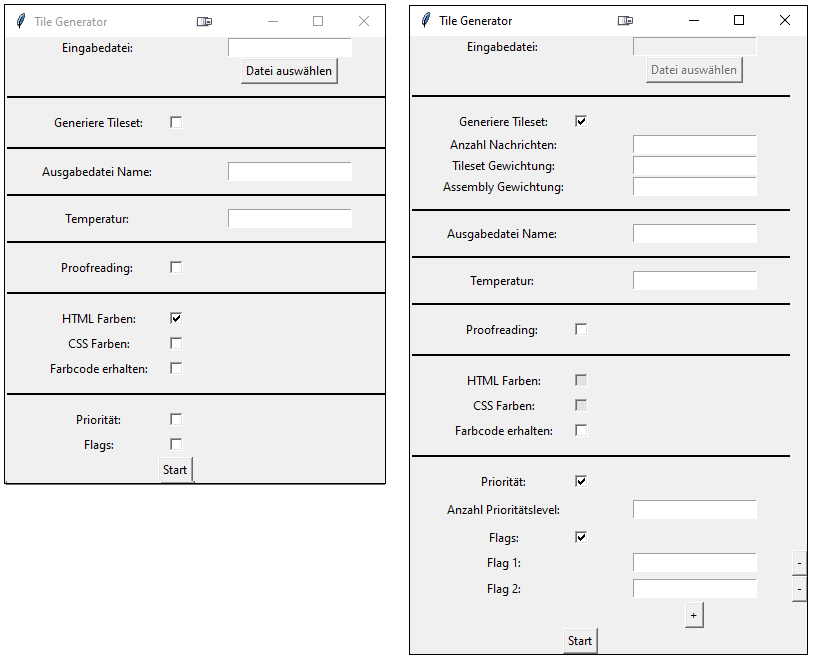
\includegraphics[width=\textwidth]{images/Tile-Generator.png}
    \caption[GUI Screenshot]{Darstellung des grafischen Interfaces des im Zuge dieser Arbeit entstandenen Skripts. Links ist dabei das Fenster ohne weitere Auswahl dargestellt. Rechts sind alle zusätzlichen Eingaben und Optionen gezeigt, die beim Auswählen aller Checkboxen hinzugefügt werden.}
    \label{fig:gui}
\end{figure}

Von Oben nach Unten sind die Einstellungsoptionen des Skripts wie folgt: Die Auswahl einer Eingabedatei fällt auf den Fall, dass ein in NetTAS erstelltes Tileset verwendet wird. Die entsprechende Datei muss über einen Datenexplorer ausgewählt werden. Wird die Checkbox \emph{Generiere Tileset} darunter ausgewählt, so öffnen sich drei Eingabefelder und eine Checkbox. Button und Eingabefeld der Eingabedatei werden dabei deaktiviert. 

In den neuen Eingabefeldern können die folgenden drei Parameter festgelegt werden: die Anzahl der Nachrichten, die durch das Tileset darstellbar sein sollen, die Gewichtung des Tileset und die Gewichtung der Self-Assembly. Alle drei Eingaben müssen ganze Zahlen beinhalten und sollte eine andere Eingabe getätigt werden, so wird diese mit einer Fehlernachricht abgefangen. Die Gewichtung von Tileset und Assembly ist relativ. Das bedeutet, dass eine Eingabe von eins in der Tileset Gewichtung und einer zehn in der Gewichtung der Assembly äquivalent zu einer Eingabe von zehn in der Tileset Gewichtung zu einer 100 in der Gewichtung der Assembly ist. Durch Aktivieren der Checkbox mit der Beschriftung \emph{Prüfsumme erstellen} wird die Prüfsummenbildung für das generierte Tileset aktiviert.

Unter dem Abschnitt zur Generierung von Tilesets findet sich das Eingabefeld der Ausgabedatei. Darin muss der Name der Datei angegeben werden. Ein \texttt{.json} am Ende des Namens ist nicht notwendig. Namen mit anderen Dateiendungen oder ohne Dateiendung werden erkannt und durch ein \texttt{.json} erweitert. Die Ausgabedatei wird immer an der gleichen Stelle im Verzeichnis wie das Skript abgespeichert.

Unter dem Eingabefeld für den Namen der Ausgabedatei ist ein weiteres Eingabefeld zu finden. Dieses dient zur Angabe der Temperatur. Auch hier kann erneut nur eine ganze Zahl angegeben werden, andere Eingaben führen zu einer Fehlermeldung. Darunter findet sich eine Checkbox mit der Beschriftung \emph{Proofreading}. Wird diese Checkbox ausgewählt, so wird auf das finale Tileset \emph{Snaked-Proofreading} angewendet.

Unter dieser Checkbox finden sich drei weitere Checkboxen. Die oberen beiden sind gegenseitig ausschließend, sodass immer nur eine aktiv sein kann. Mit ihnen kann anhand der Beschriftung angegeben werden, ob \emph{HTML Farben} oder \emph{CSS-Farben} als Farbkodierung verwendet werden. Im Fall einer Eingabedatei muss die Checkbox dem gewählten Farbschema aus dem Eingabetileset entsprechen. Ansonsten erscheint eine Fehlermeldung und das Skript kann nicht ausgeführt werden. Wird ein Tileset generiert, so sind diese beiden Checkboxen ausgegraut und nicht auswählbar, da sie keine Relevanz besitzen. Das generierte Tileset hat immer die Höhe eins und die einzige Farbkodierung ist ein Seed-Tile, das in HTML-Farbcode nach Tabelle~\ref{tab:farbkodierung} dargestellt wird. Die restlichen Tiles sind weiß codiert. Die dritte Checkbox, bezeichnet als \emph{Farbcode erhalten}, steuert die Farbkodierung des Ergebnistilesets. Ist diese Option aktiviert, bleibt die Farbkodierung im generierten Tileset bestehen. Andernfalls wird die Farbkodierung entfernt und nur die Tiles, die den Frame des Moleküls darstellen, werden in der Farbe Ozeangrün hervorgehoben, um eine bessere Übersicht zu gewährleisten. Es sei angemerkt, dass Ozeangrün die Primärfarbe des Farbschemas der Universität Lübeck ist.

Unter den drei Checkboxen für die Farbkodierung, finden sich zwei weitere Checkboxen. Die erste Checkbox für die \emph{Priorität} kann ausgewählt werden, wenn für das gegebene Tileset Prioritätstiles benötigt werden. Der genaue Ablauf wird in den folgenden Absätzen genauer betrachtet. Ist die Checkbox ausgewählt, öffnet sich ein Eingabefeld, in welchen eine ganze Zahl angegeben werden muss, um so anzugeben, wie viele Prioritätslevel es gibt. Die andere Checkbox mit dem Bezeichner \emph{Flags} öffnet beim Auswählen einen Button, der mit \glqq +\grqq~ bezeichnet wird. Durch diesen Button können beliebig viele Flags erzeugt werden, indem die dabei erscheinenden Eingabefelder mit Namen für die Tiles ausgefüllt werden. Mit dem rechts erscheinenden Button, gekennzeichnet durch ein \glqq -\grqq, kann eine falsch erstellte Flag wieder gelöscht werden. Ganz unten befindet sich der \emph{Start}-Button, der das Skript mit den oben angegeben Optionen ausführt. Danach öffnet sich der Datenexplorer an der Stelle, an der die Ausgabedatei gespeichert wird.

\section{Anforderungen für das korrekte Ausführen des Skripts}

Mit allen erforderlichen Optionen und Eingabe, können im Weiteren die Anforderungen für in NetTAS erstellte Tilesets festgelegt werden, die erfüllt werden müssen, damit das Skript funktioniert. Danach sollen auch die Anforderungen angegeben werden, die eingehalten werden sollten, um mögliche Fehler zu vermeiden. Zuletzt sollen die Anforderungen vorgestellt werden, die erfüllt werden können, um ein korrektes Skriptverhalten zu sichern.

\subsection{Notwendige Anforderungen an Tilesets}

In dieser Sektion werden die Anforderungen präsentiert, die für eine korrekte Funktionsweise des Skripts berücksichtigt werden müssen. Ein Nichtbefolgen dieser Anforderungen führt fast immer zu Fehlern. Einige dieser Fehler werden durch das Skript mit einer Fehlermeldung identifiziert, während andere zu fehlerhaften Tilesets führen können. Die erste Anforderung, das Einhalten des Farbcodes, wurde bereits bei der Beschreibung des grafischen Interfaces gegeben.

Die zweite Anforderung betrifft die Ausrichtung des Moleküls im Tileset. Das Molekül muss so konstruiert werden, dass es mit der Seed-Assembly rechts beginnt und nach links wächst. Beginnt die Seed-Assembly hingegen rechts, oben oder unten und das Molekül wächst dann in eine andere Richtung (links, unten oder oben), kann dies im Skript zu schwerwiegenden Fehlern führen.

Ein weiterer essentieller Aspekt ist die klare Definition einer Wachstumsfront an einer Molekülseite. Zur Verdeutlichung dieser Anforderung sind in Abbildung~\ref{fig:negativbsp_konstruktion} Negativbeispiele gezeigt. Es ist wichtig zu betonen, dass diese spezifische Anforderung primär im Kontext des Proofreadings relevant ist. Bei Konstruktionen ohne Proofreading könnten solche Strukturen problemlos sein. Bei Anwendung des Proofreadings ist es jedoch von zentraler Bedeutung, dass das verwendete Tileset konform mit den Wachstumsvorgaben ist. Im Proofreading-Verfahren beginnt das Wachstum stets in einem von vier festgelegten Tiles. Der Farbcode ermöglicht eine differenzierte Wachstumsdynamik in verschiedenen Molekülteilen, aber es muss stets eine konsistente Wachstumsfront beibehalten werden.

In Abbildung~\ref{fig:negativbsp_konstruktion} a) ist ein Beispiel für nicht-konformes Wachstum im Kontext des Proofreadings dargestellt. Bei Molekülen mit einer Höhe von mehr als einem Tile wird davon ausgegangen, dass das Wachstum vom Seed-Tile ausgeht. Für das in der Abbildung gezeigte Molekül wäre an der mit einem roten Kreis hervorgehobenen Position ein Kleber erforderlich.

In Abbildung~\ref{fig:negativbsp_konstruktion} b) wird ein weiteres Problem bei der Wachstumsfront dargestellt.
Für das Proofreading der zentralen Tiles bei Molekülen der Höhe drei ist es von Bedeutung, aus welcher Richtung das Wachstum erfolgt. Alle Tiles starten ihr Wachstum bei einem der vier Proofreadingtiles.
Um dies zu gewährleisten, muss eine der beiden Seiten so gebildet werden, dass sie ohne Verbindung eines zentralen Tiles auskommt. In dem dargestellten Beispiel erfordert dies das Hinzufügen von Klebern an den Stellen, die durch die blauen oder den roten Kreis markiert sind.

Das letzte Negativbeispiel ist in Abbildung~\ref{fig:negativbsp_konstruktion} c) zu sehen und ist mit dem Beispiel aus b) verbunden. In Molekülen der Höhe drei müssen die zentralen Tiles entweder von der Seed-Assembly, von der südlichen Grenze oder von der nördlichen Grenze startend wachsen. Ein Wachstum wie in c) wird durch das Skript nicht unterstützt, weshalb hier ein Kleber an einer der farbig markierten Stellen notwendig wäre.

\begin{figure}
    \centering
    \begin{tikzpicture}[scale=0.85]
        \node at (-0.4,1.7) {a)};
        \draw[fill=uzl_mediumblue_3] (0,0) rectangle (1,1);
        \draw[fill=black] (1,0.4) rectangle (1.2,0.6);
        \draw[fill=black] (2.2,0.4) rectangle (2.4,0.6);
        \draw[fill=black] (3.4,0.4) rectangle (3.6,0.6);
        \draw[fill=uzl_mediumblue_2] (1.2,0) rectangle (2.2,1);
        \draw[fill=uzl_mediumblue_2] (2.4,0) rectangle (3.4,1);
        \draw[fill=uzl_mediumblue_1] (3.6,0) rectangle (4.6,1);
        %
        \draw[fill=black] (0.4,1) rectangle (0.6,1.2);
        \draw[fill=black] (1.6,1) rectangle (1.8,1.2);
        \draw[fill=black] (2.8,1) rectangle (3,1.2);
        %
        \draw (0,1.2) rectangle (1,2.2);
        \draw[fill=black] (1,1.6) rectangle (1.2,1.8);
        \draw[fill=black] (2.2,1.6) rectangle (2.4,1.8);
        \draw[fill=black] (3.4,1.6) rectangle (3.6,1.8);
        \draw (1.2,1.2) rectangle (2.2,2.2);
        \draw (2.4,1.2) rectangle (3.4,2.2);
        \draw[fill=uzl_yellow_1] (3.6,1.2) rectangle (4.6,2.2);
        %
        \draw[fill=black] (0.4,2.2) rectangle (0.6,2.4);
        \draw[fill=black] (1.6,2.2) rectangle (1.8,2.4);
        \draw[fill=black] (2.8,2.2) rectangle (3,2.4);
        \draw[fill=black] (4,2.2) rectangle (4.2,2.4);
        %
        \draw[fill=uzl_red_3] (0,2.4) rectangle (1,3.4);
        \draw[fill=black] (1,2.8) rectangle (1.2,3);
        \draw[fill=black] (2.2,2.8) rectangle (2.4,3);
        \draw[fill=black] (3.4,2.8) rectangle (3.6,3);
        \draw[fill=uzl_red_2] (1.2,2.4) rectangle (2.2,3.4);
        \draw[fill=uzl_red_2] (2.4,2.4) rectangle (3.4,3.4);
        \draw[fill=uzl_red_1] (3.6,2.4) rectangle (4.6,3.4);
        %
        \draw[red, thick] (4.1,1.1) circle (0.3cm);
        %
        %
        %
        %
        \node at (5.4,1.7) {b)};
        \draw[fill=uzl_mediumblue_3] (5.8,0) rectangle (6.8,1);
        \draw[fill=black] (6.8,0.4) rectangle (7,0.6);
        \draw[fill=black] (9.2,0.4) rectangle (9.4,0.6);
        \draw[fill=uzl_mediumblue_2] (7,0) rectangle (8,1);
        \draw[fill=uzl_mediumblue_2] (8.2,0) rectangle (9.2,1);
        \draw[fill=uzl_mediumblue_1] (9.4,0) rectangle (10.4,1);
        %
        \draw[fill=black] (6.2,1) rectangle (6.4,1.2);
        \draw[fill=black] (7.4,1) rectangle (7.6,1.2);
        \draw[fill=black] (8.6,1) rectangle (8.8,1.2);
        \draw[fill=black] (9.8,1) rectangle (10,1.2);
        %
        \draw (5.8,1.2) rectangle (6.8,2.2);
        \draw (7,1.2) rectangle (8,2.2);
        \draw (8.2,1.2) rectangle (9.2,2.2);
        \draw[fill=uzl_yellow_1] (9.4,1.2) rectangle (10.4,2.2);
        %
        \draw[fill=black] (6.2,2.2) rectangle (6.4,2.4);
        \draw[fill=black] (7.4,2.2) rectangle (7.6,2.4);
        \draw[fill=black] (8.6,2.2) rectangle (8.8,2.4);
        \draw[fill=black] (9.8,2.2) rectangle (10,2.4);
        %
        \draw[fill=uzl_red_3] (5.8,2.4) rectangle (6.8,3.4);
        \draw[fill=black] (8,2.8) rectangle (8.2,3);
        \draw[fill=uzl_red_2] (7,2.4) rectangle (8,3.4);
        \draw[fill=uzl_red_2] (8.2,2.4) rectangle (9.2,3.4);
        \draw[fill=uzl_red_1] (9.4,2.4) rectangle (10.4,3.4);
        %
        \draw[blue, thick] (9.3,2.9) circle (0.3cm);
        \draw[blue, thick] (6.9,2.9) circle (0.3cm);
        \draw[red, thick] (8.1,0.5) circle (0.3cm);
        %
        %
        %
        %
        \node at (11.2,1.7) {c)};
        \draw[fill=uzl_mediumblue_3] (11.6,0) rectangle (12.6,1);
        \draw[fill=black] (12.6,0.4) rectangle (12.8,0.6);
        \draw[fill=black] (13.8,0.4) rectangle (14,0.6);
        \draw[fill=black] (15,0.4) rectangle (15.2,0.6);
        \draw[fill=uzl_mediumblue_2] (12.8,0) rectangle (13.8,1);
        \draw[fill=uzl_mediumblue_2] (14,0) rectangle (15,1);
        \draw[fill=uzl_mediumblue_1] (15.2,0) rectangle (16.2,1);
        %
        \draw[fill=black] (12,1) rectangle (12.2,1.2);
        \draw[fill=black] (13.2,1) rectangle (13.4,1.2);
        \draw[fill=black] (15.6,1) rectangle (15.8,1.2);
        %
        \draw (11.6,1.2) rectangle (12.6,2.2);
        \draw[fill=black] (12.6,1.6) rectangle (12.8,1.8);
        \draw[fill=black] (13.8,1.6) rectangle (14,1.8);
        \draw (12.8,1.2) rectangle (13.8,2.2);
        \draw (14,1.2) rectangle (15,2.2);
        \draw[fill=uzl_yellow_1] (15.2,1.2) rectangle (16.2,2.2);
        %
        \draw[fill=black] (12,2.2) rectangle (12.2,2.4);
        \draw[fill=black] (13.2,2.2) rectangle (13.4,2.4);
        \draw[fill=black] (15.6,2.2) rectangle (15.8,2.4);
        %
        \draw[fill=uzl_red_3] (11.6,2.4) rectangle (12.6,3.4);
        \draw[fill=black] (12.6,2.8) rectangle (12.8,3);
        \draw[fill=black] (13.8,2.8) rectangle (14,3);
        \draw[fill=black] (15,2.8) rectangle (15.2,3);
        \draw[fill=uzl_red_2] (12.8,2.4) rectangle (13.8,3.4);
        \draw[fill=uzl_red_2] (14,2.4) rectangle (15,3.4);
        \draw[fill=uzl_red_1] (15.2,2.4) rectangle (16.2,3.4);
        %
        \draw[blue, thick] (14.5,2.3) circle (0.3cm);
        \draw[green, thick] (15.1,1.7) circle (0.3cm);
        \draw[red, thick] (14.5,1.1) circle (0.3cm);
    \end{tikzpicture}
    \caption[Negativbeispiele für die Konstruktion durch das Skript]{Drei Beispiele von Tile-Assemblies, die im Skript zu Fehlern führen. Fehlen die Kleber zwischen Seedtiles und ihren nördlichen und südlichen Nachbarn, kann im Skript beim Proofreading keine korrekte Wachstumsrichtung gefunden werden. Dies ist in a) dargestellt. Auch muss entweder die nördliche Grenze oder die südliche Grenze des Moleküls durchgängig verbunden sein, da im Skript eine der beiden Seiten als Wachstumsfront definiert wird und das nicht mitten im Molekül wechseln kann. Das ist in b) zu sehen. Auch müssen alle zentralen Tiles (hier weiß codiert) von Norden, Süden oder Osten wachsen. Ein Wachstum von Westen bei zentralen Tiles ist nicht vorgesehen.}
    \label{fig:negativbsp_konstruktion}
\end{figure}

Die vierte Anforderung besagt, dass das ausgewählte Tileset für die gewählte Temperatur korrekt konstruiert sein muss. Das Skript selbst nimmt keine Korrekturen an fehlerhaften Verbindungen oder Tiles vor.

Die fünfte und abschließende Anforderung bezieht sich auf die Konsistenz von Kleberbezeichnern und Kleberstärken.Ein Tile darf auf keiner Seite einen Kleberbezeichner aufweisen, wenn dieser keine zugehörige Kleberstärke hat. Umgekehrt sollte keine Seite eines Tiles eine Kleberstärke > 0 besitzen, ohne durch einen entsprechenden Kleberbezeichner gekennzeichnet zu sein. Im Skript werden beide Werte zur Herleitung des jeweils anderen genutzt.

\subsection{Empfehlenswerte Anforderungen an Tilesets}

Im Folgenden werden empfohlene Anforderungen vorgestellt, die, obwohl nicht zwingend erforderlich, dazu beitragen, potenzielle Fehlerquellen zu minimieren. Es sollte betont werden, dass ein Nichteinhalten dieser Anforderungen nicht notwendigerweise zu Problemen führt. 

Ein zentrales Element dieser Empfehlungen ist die Notwendigkeit eines eindeutigen Bezeichners für jedes Tile. Dies ist insbesondere relevant, da beim Erstellen von Flag-, Prioritäts- und Snaked-Proofreading Tiles zusätzliche Kleberbezeichner benötigt werden. Diese werden durch Konkatenation des Tilebezeichners mit Zeichen aus einer nachfolgend dargestellten Liste generiert. Da so einige Kleberbezeichner automatisch entstehen, muss darauf geachtet werden, dass erstellte Kleberbezeichner nicht gleich heißen.
Im Skript wird für die erste Stelle der drei inneren Kleber eine kleingeschriebene Version des Tilebezeichners verwendet und danach mit drei Zeichen aus folgender Liste konkateniert:
\begin{align*}
    [0,1,\dots,8,9,a,b,\dots,y,z,aa,ab,\dots,zy,zz]
\end{align*}
Um zu verdeutlichen, wie die Kleberbezeichner generiert werden, wird das folgende Beispiel betrachtet:
\begin{description}
    \item[gegeben:]\hfill 
    \begin{itemize}
        \item vier Tiles mit dem Bezeichner $X$,
        \item ein Tile mit dem Bezeichner $Y$,
        \item zwei Tiles ohne Bezeichner.
    \end{itemize}
    \item[innere Bezeichnertripel:]\hfill
    \begin{itemize}
        \item~[$x0,x1,x2$],[$x3,x4,x5$],[$x6,x7,x8$],[$x9,xa,xb$],
        \item~[$y0,y1,y2$],
        \item~[$0,1,2$],[$3,4,5$].
    \end{itemize}
\end{description}

Dementsprechend muss beachtet werden, dass bei leeren Tilebezeichnern die generierten Kleberbezeichner einstellige Zahlen oder Buchstaben sind. Durch die Regeln der Self-Assembly kann es so beim automatischen Generieren von Kleberbezeichnern zu Wachstumsfehlern kommen. Wenn jedoch bei der Konstruktion des Tilesets in NetTAS darauf geachtet wird, muss dies keine Wachstumsfehler verursachen.

Damit verbunden sind allgemeine Regeln zur Kleberbezeichnung. Selbst wenn alle Tiles einen Bezeichner erhalten, sollte darauf geachtet werden, dass die genutzten Kleberbezeichner entweder einstellig und kleingeschrieben sind oder den folgenden Regeln entsprechen:

\begin{enumerate}
\item Bei Kleberbezeichnern mit einer Zeichenlänge von zwei oder drei darf das letzte Zeichen weder eine Zahl noch ein klein geschriebener Buchstabe sein.
\item Ein $<$ am Ende von Bezeichnern der Länge zwei kann zu Fehlern führen.
\item Kombinationen von $\{1,2\}$ am Anfang, beliebig vielen Zeichen in der Mitte und $\{F,P\}$ am Ende können von Flag- oder Prioritätstiles belegt sein.
\item Die Bezeichner $\sigma t, \sigma c$ und $\sigma b$ können belegt sein.
\item Großgeschriebene Buchstaben wie $\{A,B,\dots,Y,Z,AA,AB,\dots,ZY,ZZ\}$ werden vom Skript generiert und sollten daher nicht manuell vergeben werden.
\end{enumerate}

Während die Verwendung dieser Bezeichner nicht zwangsläufig Probleme verursacht, wird empfohlen, sie zu vermeiden, um potentiellen Fehlern vorzubeugen.

Insgesamt können durch die Zeichenmengen bis zu 237 gleich benannte Tiles unterschieden werden. Der Vollständigkeit halber muss trotzdem angemerkt werden, dass nicht mehr als 238 Mal der gleiche Tilebezeichner in einem Tileset verwendet werden sollte. 
Auch sind die Farbcodes für Flag- und Prioritätstiles im Skript zugelassen und führen nicht zu einem Error, wenn sie verwendet werden. Doch sind diese Farben nicht dafür gedacht, importiert zu werden. Sie werden im Skript als \emph{white} gewertet und müssen so platziert werden, damit es zu keinen Fehlern kommt. Es ist empfehlenswert diese Farben im gegeben Tileset nicht zu verwenden.

\subsection{Vorschläge für Tilesets}

Zuletzt werden noch einige Leitideen gegeben, denen gefolgt werden kann. Die sicherste Variante ist es, ein Tileset zu generieren. Das funktioniert bei sinnvollen und korrekten Eingaben im grafischen Interface immer fehlerfrei. Wenn jedoch ein Tileset in NetTAS erstellt wird, dann können die folgenden zwei Regeln eingehalten werden, um Fehlern vorzubeugen: Die Temperatur sollte zwischen zwei und drei gewählt werden und Tilesets für Moleküle sollten den Formen aus den Beispielen in dieser Arbeit folgen. Diese wurden alle getestet und funktionieren fehlerfrei. In Abbildung~\ref{fig:molekuel_form} sind die Molekülformen für die Höhen drei (in a,b und c), zwei ( in d und e)  und eins (in c) gegeben. All diese Strukturen wurden ausreichend getestet und funktionieren im Skript. Durch die Pfeile ist das Wachstum im Proofreading verbildlicht. Die grünen Pfeile repräsentieren die minimalen Kleberverbindungen zwischen den Molekülen. Die schwarz gestrichelten Pfeile hingegen symbolisieren zusätzliche, optionale Verbindungen. Während sie nicht zwingend für die Bildung eines Moleküls dieser Form benötigt werden, können sie dennoch notwendig sein, um eine entsprechende Berechnung in der Self-Assembly zu ermöglichen.

\begin{figure}
    \centering
    \begin{tikzpicture}[scale=0.8]
        \node at (-0.5,5.7) {a)};
        %
        \draw[fill=uzl_mediumblue_3] (0,4) rectangle (1,5);
        \draw[fill=uzl_mediumblue_2] (1.2,4) rectangle (2.2,5);
        \draw[fill=uzl_mediumblue_2] (2.4,4) rectangle (3.4,5);
        \draw[fill=uzl_mediumblue_1] (3.6,4) rectangle (4.6,5);
        %
        \draw (0,5.2) rectangle (1,6.2);
        \draw (1.2,5.2) rectangle (2.2,6.2);
        \draw (2.4,5.2) rectangle (3.4,6.2);
        \draw[fill=uzl_yellow_1] (3.6,5.2) rectangle (4.6,6.2);
        %
        \draw[fill=uzl_red_3] (0,6.4) rectangle (1,7.4);
        \draw[fill=uzl_red_2] (1.2,6.4) rectangle (2.2,7.4);
        \draw[fill=uzl_red_2] (2.4,6.4) rectangle (3.4,7.4);
        \draw[fill=uzl_red_1] (3.6,6.4) rectangle (4.6,7.4);
        %
        %
        \draw[green, thick, ->] (4.1,5.6) -- (4.1,4.5) -- (1.8,4.5);
        \draw[green, thick, ->] (4.1,5.8) -- (4.1,6.9) -- (1.8,6.9);
        \draw[green, thick, ->] (1.7,4.6) -- (1.7,5.6);
        \draw[green, thick, ->] (2.9,4.6) -- (2.9,5.6);
        \draw[green, thick, ->] (1.6,5.7) -- (0.5,5.7) -- (0.5,6.8);
        \draw[green, thick, ->] (0.5,5.7) -- (0.5,4.6);
        \draw[dashed, thick, ->] (1.6,4.5) -- (0.6,4.5);
        \draw[dashed, thick, ->] (1.6,6.9) -- (0.6,6.9);
        \draw[dashed, thick, ->] (1.7,6.8) -- (1.7,5.8);
        \draw[dashed, thick, ->] (2.9,6.8) -- (2.9,5.8);
        \draw[dashed, thick, ->] (4,5.7) -- (1.8,5.7);
        %
        %
        \node at (5.5,5.7) {b)};
        %
        \draw[fill=uzl_mediumblue_3] (6,4) rectangle (7,5);
        \draw[fill=uzl_mediumblue_2] (7.2,4) rectangle (8.2,5);
        \draw[fill=uzl_mediumblue_2] (8.4,4) rectangle (9.4,5);
        \draw[fill=uzl_mediumblue_1] (9.6,4) rectangle (10.6,5);
        %
        \draw (6,5.2) rectangle (7,6.2);
        \draw (7.2,5.2) rectangle (8.2,6.2);
        \draw (8.4,5.2) rectangle (9.4,6.2);
        \draw[fill=uzl_yellow_1] (9.6,5.2) rectangle (10.6,6.2);
        %
        \draw[fill=uzl_red_3] (6,6.4) rectangle (7,7.4);
        \draw[fill=uzl_red_2] (7.2,6.4) rectangle (8.2,7.4);
        \draw[fill=uzl_red_2] (8.4,6.4) rectangle (9.4,7.4);
        \draw[fill=uzl_red_1] (9.6,6.4) rectangle (10.6,7.4);
        %
        %
        \draw[green, thick, ->] (10.1,5.6) -- (10.1,4.5) -- (7.8,4.5);
        \draw[green, thick, ->] (10.1,5.8) -- (10.1,6.9) -- (7.8,6.9);
        \draw[dashed, thick, ->] (7.7,4.6) -- (7.7,5.6);
        \draw[dashed, thick, ->] (8.9,4.6) -- (8.9,5.6);
        \draw[green, thick, ->] (7.6,5.7) -- (6.5,5.7) -- (6.5,6.8);
        \draw[green, thick, ->] (6.5,5.7) -- (6.5,4.6);
        \draw[dashed, thick, ->] (7.6,4.5) -- (6.6,4.5);
        \draw[dashed, thick, ->] (7.6,6.9) -- (6.6,6.9);
        \draw[green, thick, ->] (7.7,6.8) -- (7.7,5.8);
        \draw[green, thick, ->] (8.9,6.8) -- (8.9,5.8);
        \draw[dashed, thick, ->] (10,5.7) -- (7.8,5.7);
        %
        %
        \node at (11.5,5.7) {c)};
        %
        \draw[fill=uzl_mediumblue_3] (12,4) rectangle (13,5);
        \draw[fill=uzl_mediumblue_2] (13.2,4) rectangle (14.2,5);
        \draw[fill=uzl_mediumblue_2] (14.4,4) rectangle (15.4,5);
        \draw[fill=uzl_mediumblue_1] (15.6,4) rectangle (16.6,5);
        %
        \draw (12,5.2) rectangle (13,6.2);
        \draw (13.2,5.2) rectangle (14.2,6.2);
        \draw (14.4,5.2) rectangle (15.4,6.2);
        \draw[fill=uzl_yellow_1] (15.6,5.2) rectangle (16.6,6.2);
        %
        \draw[fill=uzl_red_3] (12,6.4) rectangle (13,7.4);
        \draw[fill=uzl_red_2] (13.2,6.4) rectangle (14.2,7.4);
        \draw[fill=uzl_red_2] (14.4,6.4) rectangle (15.4,7.4);
        \draw[fill=uzl_red_1] (15.6,6.4) rectangle (16.6,7.4);
        %
        %
        \draw[green, thick, ->] (16.1,5.6) -- (16.1,4.5) -- (13.8,4.5);
        \draw[green, thick, ->] (16.1,5.8) -- (16.1,6.9) -- (13.8,6.9);
        \draw[dashed, thick, ->] (13.7,4.6) -- (13.7,5.6);
        \draw[dashed, thick, ->] (14.9,4.6) -- (14.9,5.6);
        \draw[green, thick, ->] (13.6,5.7) -- (12.5,5.7) -- (12.5,6.8);
        \draw[green, thick, ->] (12.5,5.7) -- (12.5,4.6);
        \draw[dashed, thick, ->] (13.6,4.5) -- (12.6,4.5);
        \draw[dashed, thick, ->] (13.6,6.9) -- (12.6,6.9);
        \draw[dashed, thick, ->] (13.7,6.8) -- (13.7,5.8);
        \draw[dashed, thick, ->] (14.9,6.8) -- (14.9,5.8);
        \draw[green, thick, ->] (16,5.7) -- (13.8,5.7);
        %
        %
        \node at (2.5,2.1) {d)};
        %
        \draw[fill=uzl_mediumblue_3] (3,1.2) rectangle (4,2.2);
        \draw[fill=uzl_mediumblue_2] (4.2,1.2) rectangle (5.2,2.2);
        \draw[fill=uzl_mediumblue_2] (5.4,1.2) rectangle (6.4,2.2);
        \draw[fill=uzl_mediumblue_1] (6.6,1.2) rectangle (7.6,2.2);
        %
        \draw (3,2.4) rectangle (4,3.4);
        \draw (4.2,2.4) rectangle (5.2,3.4);
        \draw (5.4,2.4) rectangle (6.4,3.4);
        \draw[fill=uzl_yellow_1] (6.6,2.4) rectangle (7.6,3.4);
        %
        %
        \draw[green, thick, ->] (7.1,2.8) -- (7.1,1.7) -- (4.8,1.7);
        \draw[green, thick, ->] (4.7,1.8) -- (4.7, 2.9) -- (3.5,2.9) -- (3.5,1.7);
        \draw[green, thick, ->] (5.9,1.7) -- (5.9,2.8);
        \draw[dashed, thick, ->] (7,2.9) -- (4.8,2.9);
        \draw[dashed, thick, ->] (4.6,1.7) -- (3.6,1.7);
        %
        %
        \node at (8.5,2.1) {e)};
        %
        \draw[fill=uzl_mediumblue_3] (9,1.2) rectangle (10,2.2);
        \draw[fill=uzl_mediumblue_2] (10.2,1.2) rectangle (11.2,2.2);
        \draw[fill=uzl_mediumblue_2] (11.4,1.2) rectangle (12.4,2.2);
        \draw[fill=uzl_mediumblue_1] (12.6,1.2) rectangle (13.6,2.2);
        %
        \draw (9,2.4) rectangle (10,3.4);
        \draw (10.2,2.4) rectangle (11.2,3.4);
        \draw (11.4,2.4) rectangle (12.4,3.4);
        \draw[fill=uzl_yellow_1] (12.6,2.4) rectangle (13.6,3.4);
        %
        %
        \draw[green, thick, ->] (13.1,2.8) -- (13.1,1.7) -- (10.8,1.7);
        \draw[green, thick, ->] (13, 2.9) -- (9.5,2.9) -- (9.5,1.7);
        \draw[dashed, thick, ->] (10.7,1.8) -- (10.7, 2.8);
        \draw[dashed, thick, ->] (11.9,1.7) -- (11.9,2.8);
        \draw[dashed, thick, ->] (10.6,1.7) -- (9.6,1.7);
        %
        %
        \node at (5.5,0) {f)};
        %
        \draw (6,-0.5) rectangle (7,0.5);
        \draw (7.2,-0.5) rectangle (8.2,0.5);
        \draw (8.4,-0.5) rectangle (9.4,0.5);
        \draw[fill=uzl_yellow_1] (9.6,-0.5) rectangle (10.6,0.5);
        %
        %
        \draw[green, thick, ->] (10.1,0) -- (6.6,0);
    \end{tikzpicture}
    \caption[Empfohlene Molekülformen]{Darstellung von verschiedenen Molekülformen, die empfohlen werden, um die korrekte Ausführung des Skripts zu gewährleisten. Die grünen Pfeile stellen dabei die minimal benötigten Kleber dar, die schwarz gestrichelten Pfeile sind nicht zwingend notwendig, könnten aber benötigt werden, wenn es die Logik der Assembly verlangt. a), b) und c) sind dabei verschiedene Möglichkeiten für Moleküle der Höhe drei. d) und e) sind die zwei möglichen Wachstumsrichtungen für Moleküle der Höhe zwei und f) stellt die eine triviale Wachstumsrichtung für Moleküle der Höhe eins dar.}
    \label{fig:molekuel_form}
\end{figure}

\section{Ablauf des Skripts}

Es wurden die Voraussetzungen vorgestellt, um möglichst fehlerfrei den Start-Button im grafischen Interface des Skripts drücken zu können. Damit kann im Folgenden genauer darauf eingegangen werden, was im Skript passiert, nachdem der Start-Button gedrückt wird. 

Wenn das Skript mit einer beliebigen Eingabe ausgeführt wird, erfolgt zunächst eine Prüfung der Eingabe. Dabei wird ermittelt, welche Checkboxen aktiviert wurden. Anschließend werden die zugehörigen Eingabefelder kontrolliert. So wird beispielsweise überprüft, ob die Eingabefelder von Temperatur, Nachrichtenanzahl, Tileset/Assembly Gewichtung und Priorität Zahlen sind. Für Flags, Eingabedatei und Ausgabedatei wird überprüft, ob sie nicht leer sind. Nur wenn alle Checks positiv sind, wird die Eingabe in die Main-Funktion übergeben, um dort das finale Tileset zu erstellen. Die Main-Funktion gibt das Tileset im \texttt{\_tiles} Dictionary zurück, wodurch dieses ohne weitere Änderungen in die Ausgabedatei geschrieben werden kann. Es erscheint eine Bestätigungsnachricht, dass das Skript erfolgreich ausgeführt wurde und der Datenexplorer öffnet sich am Speicherort der Ausgabedatei.

Für eine vollständig korrekte Ausführung muss noch betrachtet werden, was in der Main-Funktion passiert. Dies kann durch folgenden Pseudocode beschrieben werden: 
\begin{lstlisting}[language=python, caption={[Pseudocode der Main-Funktion des Skripts]{Pseudocode der Main-Funktion des Skripts. Es wird je nach Input eine Menge von Tiles erstellt, die für die Ausgabe vorbereitet werden. Dabei werden Informationen gesammelt, die im Code genutzt werden, um ein korrekt funktionierendes Tileset zu garantieren. Wurden in der GUI bestimmte Checkboxen aktiviert, so werden dementsprechend Flag-, Prioritäts- und Proofreadingtiles generiert.}}, label=lst:main]
def main(data, input)      
    new_tiles = []
    gatherinfo(data)
    if flags in input:
        data.add(flags)
    if priorities in input:
        data.add(priorities)
    sort(data, colorcode aus input)
    if proofreading in input:
        new_tiles = snakedproofreading(data)
    else:
        new_tiles = data 
    if not color_kept in input: 
        change_colors(new_tiles)
    return {"_tiles": new_tiles}
\end{lstlisting}

Der Hauptfunktion muss das gegebene oder generierte Tileset übergeben werden, sowie die angegebene Systemtemperatur und die Booleans für die Checkboxen im grafischen Interface. Daraufhin werden Informationen aus dem gegebenen Tileset entnommen. Dabei wird geprüft, ob das Tileset nördlich und südlich der Seed-Assembly entsprechende Tiles besitzt. Des Weiteren erfolgt die Überprüfung, ob mögliche südliche oder nördliche Grenzen innere Kleber besitzen, über die das Wachstum im Proofreading für die inneren Tiles gestartet werden kann. Zusätzlich wird der linke Kleber der Seed-Assembly vermerkt, um sicherzustellen, dass er bei der Erstellung der Flag- und Prioritätstiles erhalten bleibt. Wenn helleblaue oder hellrote Tiles existieren, werden auch ihre linken Kleber gespeichert.

In dieser Arbeit wird immer wieder von der Generierung oder Erstellung von Tiles geredet. Dies geschieht immer in einer Liste und durch eine allgemeine Definition einer \emph{generate\_tile}-Funktion. Diese Funktion gibt ein einzelnes Tile zurück, das in korrekter Darstellung nach dem Programmcode \ref{lst:tileset_json} angegeben wird. Im Folgenden ist ein Ausschnitt aus dem Skript aus Anhang \ref{app:code} \marginnote{\qrcode[height=1cm]{https://github.com/Falkenheim/Tile-Generator}} dargestellt, der jedes Mal mit passenden Parametern verwendet wird, um ein Tile zu erstellen.

\begin{lstlisting}[language=python, caption={[Codeausschnitt der \texttt{generate\_tile}-Funktion]{Die zentrale Funktion des Skriptes, mit welcher ein einzelnes Tile generiert werden kann. In \texttt{label} wird der Tilebezeichner gespeichert, im \texttt{glues}-Array die nördlichen, östlichen, südlichen und westlichen Kleber mit Bezeichner und Stärke. Dabei liegen sie auch in dieser Reihenfolge vor. Zuletzt kann noch die Füllfarbe des Tiles angegeben werden.}}, label=lst:generate_tile]
# t = tile
# l = label
# s = strength
# c = color
def generate_tile(tl, l1, s1, l2, s2, l3, s3, l4, s4, c):
    return {
        "label": tl,
        "glues": [
            {"label": l1, "strength": s1},
            {"label": l2, "strength": s2},
            {"label": l3, "strength": s3},
            {"label": l4, "strength": s4},
        ],
        "color": c
    }
\end{lstlisting}

\section{Erstellung von Flag- und Prioritätstiles}

Wenn alle Informationen gesammelt sind, dann werden Flags und Prioritätstiles erstellt. Dies passiert nur, wenn die jeweilige Checkbox ausgewählt wurde und die Eingabefelder nicht leer sind. Für alle erstellten und benannten Flags werden Tiles erstellt. 

Die Menge an benötigten Tiles ist dabei abhängig von der Höhe der Self-Assembly. Das heißt, dass aus den gesammelten Informationen entnommen wird, ob ein Tile der Farbe \emph{salmon} oder \emph{skyblue} existiert.
Diese müssen bei Existenz von Flag- oder Prioritätstiles am westlichen Kleber angepasst werden. Sie erhalten einen neuen Kleberbezeichner $\sigma t$, $\sigma c$ und $\sigma b$ für \texttt{top}, \texttt{center} und \texttt{bottom} Kleber. Somit wird in der Self-Assembly verhindert, dass sich das Molekül bindet, ohne die Flag- und Prioritätstiles hinzuzufügen. 

Auch muss beim Erstellen der Flagtiles beachtet werden, dass je nachdem, wie viele Flagtiles oder Prioritätstiles vorhanden sind, die westlichen Kleber des generierten Tiles verändert werden können. Dies ist in Abbildung \ref{fig:flag_prio_glues} dargestellt. In a) wird nur ein Flagtile ohne weitere Flag- oder Prioritätstiles erstellt. Dadurch ist der westliche Kleber des Flagtiles so gewählt, dass sich das restliche Molekül hier binden kann.
Dies ist analog für ein einzelnes Prioritätstile ohne Flag Tiles. In b) wird ein Flag- und ein Prioritätstile hinzugefügt. Dadurch braucht es einen zusätzlichen eindeutigen inneren Kleber zwischen Flag- und Prioritätstile. Der Vorgang ist wiederum analog für zwei Flagtiles. In c) ist der letzte Fall dargestellt, in welchem zwei Flagtiles und ein Prioritätstile hinzugefügt werden. Dabei werden mehrere innere Kleber benötigt. Es werden immer drei Kleberbezeichner aus der Menge $\{A,B,C,\dots,AA,AB,AC,\dots,ZX,ZY,ZZ\}$ entnommen. Somit sind bis zu 234 Flag- oder Prioritätstiles nebeneinander möglich.

\begin{figure}
    \centering
    \begin{tikzpicture}
        \tileFlagPrioZeroB{-1}{2.4}
        \tileFlagPrioZeroM{-1}{1.2}
        \tileFlagPrioZeroY{-1}{0}
        %
        \tileFlagPrioZeroA{0.2}{2.4}
        \tileFlagPrioZeroSigma{0.2}{1.2}
        \tileFlagPrioZeroX{0.2}{0}
        \node[scale=3] at (1.7,1.2) {$\Rightarrow$};
        %
        %
        %
        \node at (3,5.2) {a)};
        \tileFlagPrioOneB{4}{6.4}
        \tileFlagPrioOneM{4}{5.2}
        \tileFlagPrioOneY{4}{4}
        %
        \tileFlagPrioOneFt{5.2}{6.4}
        \tileFlagPrioOneFc{5.2}{5.2}
        \tileFlagPrioOneFb{5.2}{4}
        %
        \tileFlagPrioOneA{6.4}{6.4}
        \tileFlagPrioOneSigma{6.4}{5.2}
        \tileFlagPrioOneX{6.4}{4}
        %
        %
        %
        \node at (3,1.2) {b)};
        \tileFlagPrioTwoB{4}{2.4}
        \tileFlagPrioTwoM{4}{1.2}
        \tileFlagPrioTwoY{4}{0}
        %
        \tileFlagPrioTwoOneA{5.2}{2.4}
        \tileFlagPrioTwoOneB{5.2}{1.2}
        \tileFlagPrioTwoOneC{5.2}{0}
        %
        \tileFlagPrioTwoFt{6.4}{2.4}
        \tileFlagPrioTwoFc{6.4}{1.2}
        \tileFlagPrioTwoFb{6.4}{0}
        %
        \tileFlagPrioTwoA{7.6}{2.4}
        \tileFlagPrioTwoSigma{7.6}{1.2}
        \tileFlagPrioTwoX{7.6}{0}
        %
        %
        %
        \node at (3,-2.8) {c)};
        \tileFlagPrioThreeB{4}{-1.6}
        \tileFlagPrioThreeM{4}{-2.8}
        \tileFlagPrioThreeY{4}{-4}
        %
        \tileFlagPrioThreeOneD{5.2}{-1.6}
        \tileFlagPrioThreeOneE{5.2}{-2.8}
        \tileFlagPrioThreeOneF{5.2}{-4}
        %
        \tileFlagPrioThreeGA{6.4}{-1.6}
        \tileFlagPrioThreeGB{6.4}{-2.8}
        \tileFlagPrioThreeGC{6.4}{-4}
        %
        \tileFlagPrioThreeFt{7.6}{-1.6}
        \tileFlagPrioThreeFc{7.6}{-2.8}
        \tileFlagPrioThreeFb{7.6}{-4}
        %
        \tileFlagPrioThreeA{8.8}{-1.6}
        \tileFlagPrioThreeSigma{8.8}{-2.8}
        \tileFlagPrioThreeX{8.8}{-4}
    \end{tikzpicture}
    \caption[Kleberverhalten beim Hinzufügen von Flag- und Prioritätstiles]{Darstellung des inneren Kleberverhaltens für Flag- und Prioritätstiles. Sowohl a), b) und c) stammen original aus dem linken Molekül. In a) wird ein einzelnes Flag Tile im Molekül hinzugefügt. Dabei muss nur der Kleber an den Tiles \texttt{$\sigma$, A} und \texttt{X} geändert werden. Die Flag Tiles können dann östlich dieser Bezeichner und westlich die alten Bezeichner erhalten, an welchen \texttt{B,M} und \text{Y} gebunden werden. In b) ist das innere Kleberverhalten dargestellt. Die Kleberbezeichner \texttt{A,B,C} werden verwendet, um die Flag- und Prioritätstiles zu verbinden. Die restliche Kleberbezeichner sind analog zu a) gesetzt. In c) wird gezeigt wie die inneren Kleber sich im Weiteren verhalten. Das Flagtile mit dem Bezeichner \texttt{G} hat so komplett eigene Kleberbezeichner. Die restlichen Bezeichner sind wieder analog zu b) und a). Auch ist anzumerken, dass keine Unterscheidung in der Konstruktionsweise von zwei Flagtiles zu einem Flagtile und einem Prioritätstile gemacht wird.}
    \label{fig:flag_prio_glues}
\end{figure}

Wie angedeutet ist die Erstellung von Prioritätstiles analog zu den Flagtiles. Dabei muss nur darauf geachtet werden, ob und wie viele Flagtiles existieren, um so die korrekten östlichen Kleber erstellen zu können. Die westlichen Kleber sind immer die Kleber, die das restliche Molekül binden.

Sind Flag- und Prioritätstiles erstellt, wird zunächst das Tileset nach den Farben der Tiles sortiert. Dies wird zum einen aus Gründen der Übersicht vorgenommen, zum anderen, um sicherzustellen, dass die Seed-Assembly an erster Stelle steht. Denn so wird die Seed-Assembly in NetTAS festgelegt. Auch wird diese Sortierung bei der Anwendung von Snaked Proofreading verwendet. Wenn an dieser Stelle jedoch kein Proofreading vorgenommen werden soll, wird die Eingabemenge in die Liste \texttt{new\_tiles} übernommen. In dieser Liste wird dann noch die Farbkodierung entfernt, wenn nicht die entsprechende Checkbox ausgewählt wurde, durch die der Farbcode erhalten bleibt. Die Liste kann wie folgt zurückgegeben werden:
\begin{lstlisting}[language=python, caption={[Main-Funktion Rückgabe]{Die Rückgabe der Main-Funktion, die so erstellt wird, dass sie ohne Probleme in eine JSON-Ausgabedatei geschrieben werden kann.}}]
    return {"_tiles": new_tiles}
\end{lstlisting}

\section{Proofreading im Skript}

Wird jedoch Snaked-Proofreading auf das Tileset angewendet, dann wird die \texttt{new\_tiles}-Liste neu erstellt. Jedes Tile aus der sortierten Liste von Tiles in \texttt{data[\_tiles]} wird durch vier neue Tiles ersetzt. Dabei folgen die Tiles den Regeln des Snaked-Proofreadings aus dem Kapitel \ref{cha:grundlagen}, dargestellt in Abbildung \ref{fig:error_korrektur}. Diese vier Tiles müssen zusammen wieder die gleiche Information und Position des originalen Tiles beinhalten. 

Die so erstellten Tiles müssen dabei von einem der vier Tiles aus mit ihrem Wachstum starten. Je nach Position im Molekül kann dieses Wachstum mit einem anderen Tile starten. In Abbildung \ref{fig:snaked_wachstum} ist dies für alle farbcodierten Tiles dargestellt. 

\begin{figure}
    \centering
    \begin{tikzpicture}
        \node at (-0.8,6.6) {a)};
        \tileDirectionsLBtoRBOne{0}{7.2}{uzl_red_3}
        \tileDirectionsLBtoRBTwo{1.2}{7.2}{uzl_red_3}
        \tileDirectionsLBtoRBThree{0}{6}{uzl_red_3}
        \tileDirectionsLBtoRBFour{1.2}{6}{uzl_red_3}
        \draw[green, line width=2pt, ->] (1,6.2) -- (1,7) -- (0.2,7) -- (0.2,6.2);
        \draw[line width=2pt, ->] (2,6) -- (1.4,6);
        \draw[line width=2pt, ->] (1.2,5.2) -- (1.2,5.8);
        %
        \node at (2.2,6.6) {b)};
        \tileDirectionsLBtoRBOne{3}{7.2}{uzl_red_2}
        \tileDirectionsLBtoRBTwo{4.2}{7.2}{uzl_red_2}
        \tileDirectionsLBtoRBThree{3}{6}{uzl_red_2}
        \tileDirectionsLBtoRBFour{4.2}{6}{uzl_red_2}
        \draw[green, line width=2pt, ->] (4,6.2) -- (4,7) -- (3.2,7) -- (3.2,6.2);
        \draw[line width=2pt, ->] (5,6) -- (4.4,6);
        %
        \node at (5.2,6.6) {c)};
        \tileDirectionsLBtoRBOne{6}{7.2}{uzl_red_1}
        \tileDirectionsLBtoRBTwo{7.2}{7.2}{uzl_red_1}
        \tileDirectionsLBtoRBThree{6}{6}{uzl_red_1}
        \tileDirectionsLBtoRBFour{7.2}{6}{uzl_red_1}
        \draw[green, line width=2pt, ->] (7,6.2) -- (7,7) -- (6.2,7) -- (6.2,6.2);
        \draw[line width=2pt, ->] (7.2,5.2) -- (7.2,5.8);
        %
        \node at (-3.8,3.6) {d)};
        \tileDirectionsRTtoLTOne{-3}{4.2}{white}
        \tileDirectionsRTtoLTTwo{-1.8}{4.2}{white}
        \tileDirectionsRTtoLTThree{-3}{3}{white}
        \tileDirectionsRTtoLTFour{-1.8}{3}{white}
        \draw[green, line width=2pt, ->] (-2,4) -- (-2,3.2) -- (-2.8,3.2) -- (-2.8,4);
        \draw[line width=2pt, ->] (-1.8,5) -- (-1.8,4.4);
        %
        \node at (-0.8,3.6) {e)};
        \tileDirectionsLBtoRBOne{0}{4.2}{white}
        \tileDirectionsLBtoRBTwo{1.2}{4.2}{white}
        \tileDirectionsLBtoRBThree{0}{3}{white}
        \tileDirectionsLBtoRBFour{1.2}{3}{white}
        \draw[green, line width=2pt, ->] (1,3.2) -- (1,4) -- (0.2,4) -- (0.2,3.2);
        \draw[line width=2pt, ->] (2,3) -- (1.4,3);
        %
        \node at (2.2,3.6) {f)};
        \tileDirectionsLBtoRBOne{3}{4.2}{white}
        \tileDirectionsLBtoRBTwo{4.2}{4.2}{white}
        \tileDirectionsLBtoRBThree{3}{3}{white}
        \tileDirectionsLBtoRBFour{4.2}{3}{white}
        \draw[green, line width=2pt, ->] (4,3.2) -- (4,4) -- (3.2,4) -- (3.2,3.2);
        \draw[line width=2pt, ->] (4.2,2.2) -- (4.2,2.8);
        %
        \node at (5.2,3.6) {g)};
        \tileDirectionsLTtoLBOne{6}{4.2}
        \tileDirectionsLTtoLBTwo{7.2}{4.2}{white}
        \tileDirectionsLTtoLBFour{6}{3}{white}
        \tileDirectionsLTtoLBThree{7.2}{3}{white}
        \draw[green, line width=2pt, ->] (6.2,4) -- (7,4) -- (7,3.2) -- (6.2,3.2);
        %
        \node at (-0.8,0.6) {h)};
        \tileDirectionsRTtoLTOne{0}{1.2}{uzl_mediumblue_3}
        \tileDirectionsRTtoLTTwo{1.2}{1.2}{uzl_mediumblue_3}
        \tileDirectionsRTtoLTThree{0}{0}{uzl_mediumblue_3}
        \tileDirectionsRTtoLTFour{1.2}{0}{uzl_mediumblue_3}
        \draw[green, line width=2pt, ->] (1,1) -- (1,0.2) -- (0.2,0.2) -- (0.2,1);
        \draw[line width=2pt, ->] (2,1.2) -- (1.4,1.2);
        \draw[line width=2pt, ->] (1.2,2) -- (1.2,1.4);
        %
        \node at (2.2,0.6) {i)};
        \tileDirectionsRTtoLTOne{3}{1.2}{uzl_mediumblue_2}
        \tileDirectionsRTtoLTTwo{4.2}{1.2}{uzl_mediumblue_2}
        \tileDirectionsRTtoLTThree{3}{0}{uzl_mediumblue_2}
        \tileDirectionsRTtoLTFour{4.2}{0}{uzl_mediumblue_2}
        \draw[green, line width=2pt, ->] (4,1) -- (4,0.2) -- (3.2,0.2) -- (3.2,1);
        \draw[line width=2pt, ->] (5,1.2) -- (4.4,1.2);
        %
        \node at (5.2,0.6) {j)};
        \tileDirectionsRTtoLTOne{6}{1.2}{uzl_mediumblue_1}
        \tileDirectionsRTtoLTTwo{7.2}{1.2}{uzl_mediumblue_1}
        \tileDirectionsRTtoLTThree{6}{0}{uzl_mediumblue_1}
        \tileDirectionsRTtoLTFour{7.2}{0}{uzl_mediumblue_1}
        \draw[green, line width=2pt, ->] (7,1) -- (7,0.2) -- (6.2,0.2) -- (6.2,1);
        \draw[line width=2pt, ->] (7.2,2) -- (7.2,1.4);
    \end{tikzpicture}
    \caption[Wachstumrichtung für Tiles mit Snaked-Proofreading je nach Farbcode]{Darstellung der verschiedenen Wachstumsrichtungen von Tiles mit Snaked-Proofreading. Die Richtung ist durch die grünen Pfeile dargestellt, während durch die schwarzen Pfeile der Kleber angegeben wird, über welchen die Tiles beim Start gebunden werden. In g) ist die Seed-Assembly abgebildet, die nicht durch irgendwelche Kleberverbindungen gestartet wird. a), b) und c) sind die Tiles der nördlichen Grenze. h), i) und j) sind die Tiles der südlichen Grenze. Die drei Möglichkeiten in d), e) und f) für die weißen zentralen Tiles hängen von der Wachstumsfront während der Self-Assembly ab. d) wächst von Norden, e) von Osten und f) von Süden.}
    \label{fig:snaked_wachstum}
\end{figure}

Die Seed-Assembly wird als einziges Tile aus \glqq Nichts\grqq\, gebildet und ist dementsprechend an keine Regel gebunden, wenn es um die Wachstumsrichtung geht. Im Skript wurde diese Wachstumsrichtung gewählt, da in NetTAS, dass erste angegebene Tile als neues Seedtile dient. Da dies das linksobere Tile im Proofreading ist, kann somit die in Abbildung~\ref{fig:snaked_wachstum} g) dargestellte Richtung verwendet werden. 

Das hellrote Tile nördlich des Seedtiles muss das Wachstum mit dem Tile rechts unten starten. Der Grund dafür ist, dass sobald die beiden linken Tiles gebunden sind, die roten Tiles daneben gebunden werden können. Das soll aber erst passieren, wenn alle hellroten Tiles gebunden sind. Somit müssen zuerst die beiden rechten und danach die beiden linken Tiles gebunden werden.Die Kleber zwischen Seedtiles und den nördlichen Tiles müssen so angepasst werden, dass die rechten Tiles sich verbinden können. Gleichzeitig muss die Kleberstärke zwischen den linken Tiles so gewählt werden, dass sie sich erst dann verbinden, wenn alle drei anderen hellroten Tiles bereits gebunden sind. Die roten Tiles bilden die nördliche Grenze des Moleküls. Für sie gilt dieselbe Wachstumsrichtung. Nur der Kleber, über welchen das erste Tile gebunden wird, ist in diesem Fall östlich, statt südlich. Die dunkelroten Tiles repräsentieren die nördlichen Liganden. Es wird davon ausgegangen, dass sie sich erst dann bilden, wenn das gesamte Molekül korrekt verbunden ist. Dementsprechend wächst dieses zwar genau wie das hellrote und rote Tile, jedoch benötigt das erste Tile sowohl den östlichen als auch den südlichen Kleber dafür. Wenn ein Kleber auf einer Seite fehlt, muss der jeweils andere Kleber ausreichend stark sein, um die korrekte Bindung sicherzustellen.

Für die hellblauen, blauen und dunkelblauen Tiles ist dieses Verhalten analog zu den roten, nur dass das 
Wachstum mit den oberen Tiles starten muss, da die Tiles nach Süden wachsen müssen. Diese Tiles werden immer genau gleich gebildet. Jedoch hat nicht jedes durch Self-Assembly gebildete Molekül die gleiche Höhe. Dementsprechend müssen die inneren Tiles (weiß) immer abhängig von den Informationen über das Tileset gebildet werden. Auch kann es bei Molekülen der Höhe drei zu dem Problem kommen, dass sowohl der nördliche als auch der südliche Kleber benötigt wird, um ein Tile zu binden. Da beim Snaked-Proofreading jedoch zwei Tiles gebunden werden müssen, bevor südliche und nördliche Kleber verbunden werden, könnte Information verloren gehen. 

Das beschriebene Problem ist in Abbildung~\ref{fig:assembly_problem} aufgezeichnet. Dabei ist in a) eine Self-Assembly abgebildet, die bei Snaked-Proofreading ein Problem verursacht. Die inneren und weißen Tiles sind abhängig vom südlichen und nördlichen Tile.
Je nach nördlichem Kleber des Tiles \texttt{Y} und südlichem Kleber des Tiles \texttt{B} bindet sich ein anderes zentrales Tile. 

In b) kann das Problem erkannt werden, das entsteht, wenn auf solchen Tilesets Snaked-Proofreading angewendet wird. Das Wachstum der vier zentralen Tiles startet unten rechts. Damit sich dieses Tile bindet, muss der Kleber verstärkt werden. Dadurch kann sich jedoch ein falsches Tile binden, da noch keine Information des nördlichen Klebers verwendet wird. In b) bindet sich das Tile \texttt{0}. Damit gibt es im Tileset kein Tile mehr, das sich oben rechts binden kann. Die einzigen potenziellen Kandidaten sind über dem Molekül dargestellt. Die roten Markierungen weisen dabei darauf hin, weshalb auch diese Tiles nicht gebunden werden können.

Um das Problem zu lösen, muss wie in c) dargestellt, die Information des südlichen Klebers weitergegeben werden. Durch die Konkatenation mit dem Zeichen \glqq <\grqq\,wird sichergestellt, dass keine falsche Bindung entstehen kann. Die Information des südlichen Klebers wird dabei im inneren Kleber des Proofreadings mitgegeben. Somit kann sich das \glqq falsche\grqq\, Tile unten rechts bilden, ohne ein Problem zu verursachen. Das korrekte Tile bindet sich immer oben rechts.

\begin{figure}
    \centering
    \begin{tikzpicture}[scale=0.9]
        \node at (-6.2,3) {a)};
        \tileSPProblemBZero{-3.4}{6}
        \tileSPProblemYOne{-3.4}{0}
        \tileSPProblemOneBot{-5.2}{4.5}
        \tileSPProblemZero{-5.2}{3}
        \tileSPProblemTwo{-5.2}{1.5}
        %
        \tileSPProblemBOne{-3.4}{4.2}
        \tileSPProblemOneTop{-3.4}{3}
        \tileSPProblemYZero{-3.4}{1.8}
        %
        \tileSPProblemA{-2.2}{4.2}
        \tileSPProblemSigma{-2.2}{3}
        \tileSPProblemX{-2.2}{1.8}
        %
        %
        %
        \tileSPProblemSnakedZeroRT{0.3}{7.6}
        \draw[red, thick] (0.3,7.95) circle (0.2cm);
        \tileSPProblemSnakedOneTRT{1.8}{7.6}
        \draw[red, thick] (1.8,7.2) circle (0.2cm);
        \tileSPProblemSnakedTwoRT{3.3}{7.6}
        \draw[red, thick] (3.3,7.2) circle (0.2cm);
        %
        \node at (-1,3) {b)};
        \tileSPProblemSnakedBOneLT{0}{6}
        \tileSPProblemSnakedBOneRT{1.2}{6}
        \tileSPProblemSnakedBOneLB{0}{4.8}
        \tileSPProblemSnakedBOneRB{1.2}{4.8}
        %
        \tileSPProblemSnakedZeroRB{1.2}{2.4}
        %
        \tileSPProblemSnakedYZeroLT{0}{1.2}
        \tileSPProblemSnakedYZeroRT{1.2}{1.2}
        \tileSPProblemSnakedYZeroLB{0}{0}
        \tileSPProblemSnakedYZeroRB{1.2}{0}
        %
        \tileSPProblemSnakedALT{2.4}{6}
        \tileSPProblemSnakedART{3.6}{6}
        \tileSPProblemSnakedALB{2.4}{4.8}
        \tileSPProblemSnakedARB{3.6}{4.8}
        %
        \tileSPProblemSnakedSigmaLT{2.4}{3.6}
        \tileSPProblemSnakedSigmaRT{3.6}{3.6}
        \tileSPProblemSnakedSigmaLB{2.4}{2.4}
        \tileSPProblemSnakedSigmaRB{3.6}{2.4}
        %
        \tileSPProblemSnakedXLT{2.4}{1.2}
        \tileSPProblemSnakedXRT{3.6}{1.2}
        \tileSPProblemSnakedXLB{2.4}{0}
        \tileSPProblemSnakedXRB{3.6}{0}
        %
        %
        %
        %
        \node at (5,3) {c)};
        \tileSPProblemSnakedBOneLT{6}{6}
        \tileSPProblemSnakedBOneRT{7.2}{6}
        \tileSPProblemSnakedBOneLB{6}{4.8}
        \tileSPProblemSnakedBOneRB{7.2}{4.8}
        %
        \tileSPProblemSnakedOneTLT{6}{3.6}
        \tileSPProblemSnakedOneTRTFix{7.2}{3.6}
        \tileSPProblemSnakedOneTLB{6}{2.4}
        \tileSPProblemSnakedZeroRBFix{7.2}{2.4}
        %
        \tileSPProblemSnakedYZeroLT{6}{1.2}
        \tileSPProblemSnakedYZeroRT{7.2}{1.2}
        \tileSPProblemSnakedYZeroLB{6}{0}
        \tileSPProblemSnakedYZeroRB{7.2}{0}
        %
        \tileSPProblemSnakedALT{8.4}{6}
        \tileSPProblemSnakedART{9.6}{6}
        \tileSPProblemSnakedALB{8.4}{4.8}
        \tileSPProblemSnakedARB{9.6}{4.8}
        %
        \tileSPProblemSnakedSigmaLT{8.4}{3.6}
        \tileSPProblemSnakedSigmaRT{9.6}{3.6}
        \tileSPProblemSnakedSigmaLB{8.4}{2.4}
        \tileSPProblemSnakedSigmaRB{9.6}{2.4}
        %
        \tileSPProblemSnakedXLT{8.4}{1.2}
        \tileSPProblemSnakedXRT{9.6}{1.2}
        \tileSPProblemSnakedXLB{8.4}{0}
        \tileSPProblemSnakedXRB{9.6}{0}
    \end{tikzpicture}
    \caption[Snaked-Proofreading Problem für Moleküle der Höhe drei.]{Darstellung eines Problems von Snaked-Proofreading bei Molekülen der Höhe drei. In a) ist ein solches Molekül dargestellt. Abhängig vom südlichen Kleber von Tile \texttt{B} und dem nördlichen Kleber von Tile \texttt{Y} existieren die vier unterschiedlichen Tiles: \texttt{0,1,1} und \texttt{2}. Das Tile mit dem Bezeichner \texttt{1} gibt es dabei zweimal, da einmal die \texttt{1} von oben und einmal von unten geliefert wird. In b) kann das Problem bei dieser Self-Assembly erkannt werden. Da das zentrale Tile an der unteren rechten Seite das Wachstum starten muss, ist dort der Kleber stärker. So kann sich das Tile \texttt{0} binden und bei Temperatur drei halten. Jedoch müsste sich zur korrekten Bindung das Tile \texttt{1} binden. Es kann sich jedoch kein weiteres Tile binden, wie durch die rote Markierung darüber dargestellt wurde. Die Lösung für das Problem wird in c) dargestellt. Der Kleberbezeichner im Süden der Tiles (\texttt{0} bei Tiles \texttt{1} und \texttt{0} und \texttt{1} bei Tiles \texttt{1} und \texttt{2}) muss nach oben weitergegeben werden. Dafür wird der Bezeichner mit \texttt{<} konkateniert. Damit bindet sich rechtsoben das richtige Tile. Auch wenn unten \texttt{0} gebunden wird, kann durch die Weitergabe der \texttt{0} an den nördlichen Kleber, das korrekte Tile darüber gebunden werden.}
    \label{fig:assembly_problem}
\end{figure}

Wie in Abbildung~\ref{fig:snaked_wachstum} dargestellt wird, gibt es je nach Existenz der jeweiligen Tiles drei mögliche Wachstumsrichtungen. Gibt es blaue Tiles, die alle nördliche Kleber besitzen, so wachsen die inneren Tiles vom südlichen Kleber des rechten unteren Tiles aus. Das ist in Abbildung~\ref{fig:snaked_wachstum} f) dargestellt. Gibt es keine blauen Tiles im Tileset oder haben nicht alle blauen Tiles nördliche Kleber, so wird überprüft, ob es rote Tiles gibt. Falls alle diese Tiles einen südlichen Kleber besitzen, beginnt das Wachstum der inneren Tiles vom nördlichen Kleber aus, wobei mit dem rechtsoberen Tile gestartet wird. Das wird in Abbildung~\ref{fig:snaked_wachstum} d) gezeigt. Gilt keiner der beiden genannten Fälle, so müssen die inneren Tiles von der Seed-Assembly aus gebildet werden. Dabei wachsen die vier Tiles vom linken unteren Tile und dessen östlichem Kleber aus. Dies ist in Abbildung~\ref{fig:snaked_wachstum} e) zu sehen.

Damit sind alle Regeln für das Bilden der Tiles ausgelegt. So können die vier Tiles durch die entsprechenden Abfragen generiert werden. Für jedes Tile werden diese in der \texttt{new\_tiles}-Liste gesammelt. Sind alle Schritte und Funktionen aus Code~\ref{lst:main} durchlaufen, so wird der Inhalt in eine JSON-Datei geschrieben, die in NetTAS geladen und simuliert werden kann. 

In diesem Kapitel wurde die Konstruktion des Python-Skripts vorgestellt, mit welchem einige der Mechanismen aus dem vorherigen Kapitel in Tilesets implementiert werden. Auch wurde näher beschrieben, wie diese Mechanismen sinnvoll in Tilesets eingebaut werden können. Mit dem Skript und der Vorstellung dieser Mechanismen können im Weiteren Simulationen durchgeführt und die Ergebnisse evaluiert werden.
	\chapter{Simulationen}
\label{cha:simulationen}

In diesem Kapitel steht nach der Darstellung von Konzept und Struktur der Anforderungen die Evaluation der Simulationsergebnisse an. Einige dieser Ergebnisse werden mithilfe von Boxplots präsentiert, da diese eine umfassende Darstellung der Messwerte ermöglichen: Sie zeigen das Minimum und Maximum sowie den Median und die Quartile. Dadurch wird die gesamte Messreihe kompakt dargestellt. Die vorgestellte Simulationsumgebung NetTAS dient zur Generierung der Messergebnisse. Zunächst wird die Gewichtung bei der Generierung von Tilesets untersucht. Danach werden für acht durch das Skript generierte und in NetTAS erstellte Tilesets Simulation und Evaluation von Acknowledgements, Prioritätleveln, Flags, Prüfsummen und Snaked-Proofreading durchgeführt.

\section{Simulation und Evaluation der Gewichtungen zur Generierung von Tilesets}

Zur Evaluation und Analyse der im vorherigen Kapitel vorgestellten und implementierten Anforderungen werden Tilesets zur Simulation und Evaluation benötigt. Vier Tilesets wurden in NetTAS erstellt. Diese Tilesets werden später in diesem Kapitel noch genauer beschrieben. Vier weitere Tilesets wurden mit dem Skript generiert. Bei der Beschreibung des Vorgangs im vorherigen Kapitel wurde jedoch eine sinnvolle Gewichtung zwischen Tileset- und Assemblygröße offengelassen.

So muss zunächst die Generierung von Tilesets analysiert werden. Da die Tilegenerierung von drei Faktoren abhängt, müssen diese zuerst betrachtet und analysiert werden. Die Anzahl an Nachrichten in einem System ist zwar eine anwendungsabhängige Eingabe, jedoch muss für unterschiedlich große Nachrichtensätze gute Gewichtungen von Tileset und Assembly gefunden werden. Dabei ist erneut anzumerken, dass eine \glqq gute Gewichtung\grqq\, anwendungsabhängig sein kann.

Eine gute Gewichtung wird hier durch die Simulationsumgebung NetTAS gefunden, indem das Tileset und die Self-Assembly in \texttt{kTAM} simuliert wird. In \texttt{kTAM} wird durch die Bond Breaking Cost und Binding Cost definiert, wie sich ein zufällig an einer Stelle der Self-Assembly gebundenes Tile bindet oder löst. Dies ist in der Simulation abhängig von der Größe der Self-Assembly, da so mehr mögliche Wachstumsfronten entstehen. Auch die Größe des Tilesets beeinflusst die Simulation, da häufiger \glqq falsche\grqq\, Bindungen getestet werden. 


\begin{figure}
    \centering
    \begin{subfigure}[b]{0.49\textwidth}
        \begin{tikzpicture}[scale=0.8]
        \plottingTilesetWeights
        {40}{1}{70}
        {40}{1}{15}
        {(1.0,10)(2.0,10)(3.0,12)(40.0,12)}
        {(1.0,4)(2.0,4)(3.0,3)(40.0,3)}
        \end{tikzpicture}
        \caption{Nachrichtenanzahl = 10}
    \end{subfigure}
    \hfill
    \begin{subfigure}[b]{0.49\textwidth}
        \begin{tikzpicture}[scale=0.8]
        \plottingTilesetWeights
        {40}{1}{70}
        {40}{1}{15}
        {(1.0,17)(5.0,17)(6.0,22)(40.0,22)}
        {(1.0,5)(5.0,5)(6.0,4)(40.0,4)}
        \end{tikzpicture}
        \caption{Nachrichtenanzahl = 100}
    \end{subfigure}
    \hfill
    \begin{subfigure}[b]{0.49\textwidth}
        \begin{tikzpicture}[scale=0.8]
        \plottingTilesetWeights
        {40}{1}{70}
        {40}{1}{15}
        {(1.0,22)(4.0,22)(5.0,26)(6.0,26)(7.0,32)(34.0,32)(35.0,66)(40.0,66)}
        {(1.0,7)(4.0,7)(5.0,6)(6.0,6)(7.0,5)(34.0,5)(35.0,4)(40.0,4)}
        \end{tikzpicture}
        \caption{Nachrichtenanzahl = 1000}
    \end{subfigure}
    \hfill
    \begin{subfigure}[b]{0.49\textwidth}
        \begin{tikzpicture}[scale=0.8]
        \plottingTilesetWeights
        {40}{1}{70}
        {40}{1}{15}
        {(1.0,30)(2.0,30)(3.0,32)(5.0,32)(6.0,42)(26.0,42)(27.0,68)(40.0,68)}
        {(1.0,9)(2.0,9)(3.0,8)(5.0,8)(6.0,6)(26.0,6)(27.0,5)(40.0,5)}
        \end{tikzpicture}
        \caption{Nachrichtenanzahl = 10000}
    \end{subfigure}
    \hfill
    \begin{subfigure}[b]{0.49\textwidth}
        \begin{tikzpicture}[scale=0.8]
        \plottingAssemblyWeights
        {40}{1}{70}
        {40}{1}{15}
        {(1.0,17)(3.0,17)(4.0,16)(40.0,16)}
        {(1.0,5)(3.0,5)(4.0,9)(40.0,9)}
        \end{tikzpicture}
        \caption{Nachrichtenanzahl = 100}
    \end{subfigure}
    \hfill
    \begin{subfigure}[b]{0.49\textwidth}
        \begin{tikzpicture}[scale=0.8]
        \plottingAssemblyWeights
        {40}{1}{70}
        {40}{1}{15}
        {(1.0,30)(2.0,29)(40.0,29)}
        {(1.0,9)(2.0,11)(40.0,11)}
        \end{tikzpicture}
        \caption{Nachrichtenanzahl = 10000}
    \end{subfigure}
    \caption[Graphen zur Relation von Gewichtungen zur Nachrichtenmenge]{Graphen zur Relation von Gewichtungen und Anzahl von zu codierenden Nachrichten. Die Anzahl der Nachrichten ist unter den Graphen abgebildet. Die Graphen (a) bis (d) stellen die Tileset:Assembly Gewichtung mit wachsender Tileset-Gewichtung dar, (e) und (f) mit wachsender Assembly-Gewichtung. In den Graphen ist die Tilesetgröße an der linken y-Achse und Assemblygröße an der rechten y-Achse dargestellt.}
    \label{fig:eval_gewichtungen}
\end{figure}

Dieser Faktor ist eine der größten Schwächen von \texttt{kTAM}, da in einer realitätsnäheren Betrachtung nicht immer nur ein zufälliges Tile an einer zufälligen Stelle versucht eine Bindung aufzubauen. In der Realität läuft dies parallel an allen Stellen mit mehreren Tiles ab. Doch für die Betrachtung und Analyse der Gewichtungen von Tileset und Assembly hilft es dabei eine Argumentationsbasis aufzubauen. Braucht kTAM bedeutend länger für die Bildung einer Self-Assembly, dann kann davon ausgegangen werden, dass die Gewichtung falsch gewählt wurde, weil entweder die Assembly oder das Tileset in Relation zum jeweils anderen zu groß gewählt wurde. 

Mit dieser Information können Tilesets mit unterschiedlichen Gewichtungen erstellt werden. Dafür werden verschiedene Nachrichtenanzahlen verwendet und durch unterschiedliche Gewichtungen auf die Größe von Tileset und Assembly getestet. Dies ist in Abbildung~\ref{fig:eval_gewichtungen} abgebildet. "In Abbildung 6.1 wird die Gewichtung zwischen Tileset und Assembly dargestellt. Für das Tileset-Gewicht wird ein Spektrum bis zu einer Gewichtung von 100:1 im Vergleich zur Assembly untersucht. Umgekehrt wird für das Assembly-Gewicht eine Betrachtung bis zu einer Gewichtung von 1:100 vorgenommen. Gewichtungen darüber werden nicht betrachtet. Die Temperatur des Systems wird auf zwei festgelegt.

Aus der Abbildung~\ref{fig:eval_gewichtungen} lässt sich entnehmen, welche Gewichtungen für eine gegebene Nachrichtenmenge angemessen sind. Bei einer kleinen Nachrichtenmenge machen Verhältnisse wie $1:4$ und $1:40$ keinen Unterschied, daher genügt die Simulation eines Verhältnisses. Aus den Abbildungen zeigt sich, dass für Nachrichtenanzahlen unter $1000$ relativ ähnliche Verhältnisse getestet werden können. Bei höheren Nachrichtenzahlen sollte ein größeres Verhältnis berücksichtigt werden. Gemäß den Gewichtungen aus Abbildung~\ref{fig:eval_gewichtungen} e) und f) erhält das Tileset ein größeres Gewicht als die Assembly. Sowohl bei kleinen als auch großen Nachrichtenmengen bleibt die Größe des Tilesets und der Assembly für bereits geringe Verhältnisse konstant. Alle sechs Graphen bilden das Verhältnis zwar nur bis zur Gewichtung von \texttt{40:1}, beziehungsweise \texttt{1:40} ab, jedoch wurden alle Verhältnisse bis zu der Gewichtung \texttt{1:100} und \texttt{100:1} getestet. In keinem der Fälle gab es zwischen $40$ und $100$ weitere Veränderungen in Tileset- und Assemblygröße. So werden nun folgende Simulationen durchgeführt, um eine sinnvolle Gewichtung von Tileset- und Assemblygröße für den Rest der Evaluation zu finden. Dafür werden die Nachrichtenmengen und Gewichtungen wie folgt gewählt:
\begin{description}
    \item[Nachrichtenmenge $10$:] \texttt{1:1, 1:3, 4:1}
    \item[Nachrichtenmenge $100$:] \texttt{1:1, 1:5, 1:6, 4:1}
    \item[Nachrichtenmenge $1.000$:] \texttt{1:1, 1:5, 1:7, 1:35, 2:1}
    \item[Nachrichtenmenge $10.000$:] \texttt{1:3, 1:6, 1:27, 1:1, 2:1}
\end{description}


\begin{table}
    \centering
    \begin{tabular}{lrrrr}
         & \multicolumn{4}{c}{Nachrichtenmenge} \\
        Verhältnis & 10 & 100 & 1.000 & 10.000\\\hline 
        \texttt{4:1} & 122 & 1.425 &  &  \\
        \texttt{2:1} &  &  & 735 & 3.153 \\
        \texttt{1:1} & \underline{106} & 335 & 1249 &  \\
        \texttt{1:3} & 109 &  &  & 1.316 \\
        \texttt{1:5} &  & 353 & 1.038 &  \\
        \texttt{1:6} &  & \underline{250} &  & 1.214 \\
        \texttt{1:7} &  &  & \underline{531} &  \\
        \texttt{1:27} &  &  &  & \underline{1.021} \\
        \texttt{1:35} &  &  & 721 &   \\\hline
    \end{tabular}
    \caption[Simulationsergebnisse für verschiedene Gewichtungsverhältnisse]{Darstellung des Medians der Messergebnisse in \texttt{kTAM} für verschiedene Verhältnisse (Tileset:Assembly), die aus Abbildung~\ref{fig:eval_gewichtungen} entnommen wurden. Zur Berechnung der dargestellten Werte wurden 20 Simulationsdurchläufe in \texttt{kTAM} durchgeführt. Angesichts signifikanter Ausreißer wurde der Median für alle 20 Durchläufe bestimmt und dann die 15 \% der Messungen mit dem größten Abstand zum Median ausgeschlossen. Nachdem so die drei größten Ausreißer entfernt wurden, wurde der Median der verbleibenden 17 Messungen genommen. Diese Ergebnisse sind hier abgebildet. Für jede Nachrichtenmenge wurde die niedrigste Messung unterstrichen.}
    \label{tab:eval_weights}
\end{table}

Für die Messungen in Tabelle~\ref{tab:eval_weights} wurden 20 Messungen in \texttt{kTAM} durchgeführt. Die generierten Daten wurden mit Temperatur zwei erstellt und die dafür gewählten Parameter in \texttt{kTAM} sind wie folgt gewählt:
\begin{description}
    \item[Sleep Time:] $10$
    \item[Forward Rate:] $10$
    \item[Binding Cost:] $16$ 
    \item[Bond Breaking Cost:] $11$
\end{description}
Die Werte für \emph{Binding Cost} und \emph{Bond Breaking Cost} sind passend zur Temperatur zwei gewählt. Um größere Moleküle in realistischer Zeit simulieren zu können, müssen die Kosten für die Bindung von Tiles in einem System der Temperatur zwei unter $20$ gewählt werden. Jede niedriger der Wert, desto wahrscheinlicher bindet und hält sich jedoch eine Verbindung mit Stärke eins. Dementsprechend darf der Wert nicht zu niedrig sein, da sonst fehlerhafte Verbindungen entstehen können. Bei Kosten zum Brechen von Verbindungen von über elf wird gewährleistet, dass Verbindungen der Stärke eins schnell wieder getrennt werden. Gleichzeitig brechen Verbindungen der Stärke zwei nur selten, wodurch auch größere Moleküle stabil gebunden werden können. Auch folgt aus niedrigerer \emph{Binding Cost} und höherer \emph{Bond Breaking Cost} eine geringe Zahl von Ausreißern im \emph{kTAM}. Somit kann ein leicht angepasster Median auf die Messungen angewandt werden. Bei 20 Messungen kann ein Cutoff von 15 \% für den Median gewählt werden. So wird zunächst der Median der gesamten Messreihe berechnet. Für den Cutoff werden die drei Messwerte aus der Reihe entfernt, die den größten Abstand zum Median haben. Aus den restlichen 17 Messwerten wird erneut der Median berechnet. Aus den Messungen in Tabelle~\ref{fig:eval_gewichtungen} kann gelesen werden, dass sich das Verhältnis in Relation zur Nachrichtenmenge verhält. Bei einer großen Nachrichtenmenge (hier: $10000$) sollte ein Verhältnis gewählt werden, das die Größe der Assembly stärker gewichtet. Bei kleinen Nachrichtenmengen kann dieses Verhältnis kleiner gewählt werden. Jedoch sollte trotzdem die Assembly ein klar größeres Gewicht haben. Nur bei kleinen Nachrichtenmengen kann die Gewichtung gleichmäßig gewählt werden. Dem Tileset ein höheres Gewicht zuzuordnen, ist für keine der gegebenen Nachrichtenmengen ratsam. Ein solches Vorgehen würde in der Simulation zu einer erhöhten Anzahl an Schritten führen.

\section{Die Tilesets}

Mit diesen ersten Simulationsergebnissen können im Folgenden Datensätze generiert werden, um die Mechanismen aus Kapitel~\ref{cha:konzept} simulieren und evaluieren zu können. Um alle Anforderungen vergleichen zu können, werden die acht Tilesets erstellt, die in Abbildung~\ref{fig:sim_assemblies} dargestellt werden. Ihre Parameter und Eigenschaften sind in Tabelle~\ref{tab:eval_gen_tilesets} und Tabelle~\ref{tab:eval_build_tilesets} abgebildet. 

\begin{table}
    \centering
    \begin{tabular}{lrrrr}
        Name & \texttt{H-1-mini} & \texttt{H-1-klein} & \texttt{H-1-norm} & \texttt{H-1-groß} \\\hline
        Tilset Größe & 10 & 22 & 32 & 68 \\[1ex]
        Assembly Höhe & 1 & 1 & 1 & 1 \\[1ex]
        Assembly Länge & 4 & 4 & 5 & 5 \\[1ex]
        Nachrichtenanzahl & 10 & 100 & 1000 & 10000 \\
        \multirow{2}{*}{Tileset:Assembly} & \raisebox{-2.2ex}{1:1} & \raisebox{-2.2ex}{1:6} & \raisebox{-2.2ex}{1:7} & \raisebox{-2.2ex}{1:27}\\[0.7ex]
        Gewichtung\\\hline
    \end{tabular}
    \caption[Automatisch generierte Tilesets für Simulation und Analyse]{Darstellung der in diesem Kapitel zur Simulation verwendeten Tilesets mit einigen Parametern. Die Tilesets in dieser Tabelle sind alle durch das vorgestellte Skript generiert worden und haben dementsprechend in der Assembly eine Höhe von eins. Die nicht generierten Tilesets sind in Tabelle~\ref{tab:eval_build_tilesets} dargestellt.}
    \label{tab:eval_gen_tilesets}
\end{table}

\begin{table}
    \centering
    \begin{tabular}{lrrrr}
        Name & \texttt{H-2-klein} & \texttt{H-2-norm} & \texttt{H-3-klein} & \texttt{H-3-norm}\\\hline
        Tilset Größe & 6 & 22 & 9 & 26 \\[1ex]
        Assembly Höhe & 2 & 2 & 3 & 3 \\[1ex]
        Assembly Länge & 3 & 5 & 3 & 5 \\\hline
    \end{tabular}
    \caption[In NetTAS erstellte Tilesets für Simulation und Analyse]{Darstellung der in diesem Kapitel zur Simulation verwendeten Tilesets mit einigen Parametern. Die Tilesets in dieser Tabelle wurden alle in NetTAS erstellt. Die generierten Tilesets sind in Tabelle~\ref{tab:eval_gen_tilesets} dargestellt.}
    \label{tab:eval_build_tilesets}
\end{table}

Die Tilesets wurden aus folgenden Gründen ausgewählt: Im Sinne des im vorherigen Kapitel vorgestellten Skriptes werden nur Moleküle erstellt und getestet, die durch das Skript entweder generiert oder erweitert werden können. Somit werden Tilesets für Assemblies der Höhe ein, zwei und drei erstellt. Für die Höhe zwei und drei wird jeweils ein Tileset mit minimalen Tiles erstellt und ein Tileset mit einigen Variationsmöglichkeiten in der finalen Assembly. Für die Moleküle der Höhe eins werden vier verschiedene Größen in Hinsicht auf die Nachrichtenanzahl generiert und für weitere Simulationen verwendet. 

Die Eigenschaften der Tilesets können in den Simulationsergebnissen von 2HAM dargestellt werden. Diese Ergebnisse sind in Tabelle~\ref{tab:2HAM_assemblies} dargestellt. Aus der Tabelle lassen sich die maximalen Assemblygrößen für alle Tilesets ablesen. Auch kann bei der jeweils maximalen Größe die Anzahl an verschiedenen Assemblies erkannt werden, die durch das Tileset gebildet werden können.

\begin{table}
    \begin{tabular}{lrrrrrrrr}
        Größe & 1-mini & 1-klein & 1-norm & 1-groß & 2-klein & 2-norm & 3-klein & 3-norm\\\hline
        1 & 10 & 22  & 32   & 68    & 6 & 22 & 9 & 26\\
        2 & 24 & 120 & 220  & 1012  & 3 & 25 & 5 & 26\\
        3 & 32 & 200 & 1200 & 11616 & 1 & 39 & 3 & 29\\
        4 & 16 & 100 & 2000 & 21296 & 1 & 39 & 2 & 36\\
        5 & -  & -   & 1000 & 10648 & 1 & 36 & 1 & 68\\
        6 & -  & -   & -    & -     & 1 & 36 & 1 & 128\\
        7 & -  & -   & -    & -     & 1 & 27 & 1 & 200\\
        8 & -  & -   & -    & -     & 1 & 27 & 2 & 288\\
        9 & -  & -   & -    & -     & - & 27 & 1 & 400\\
        10 & - & -   & -    & -     & - & 27 & - & 672\\
        11 & - & -   & -    & -     & - & -  & - & 960\\
        12 & - & -   & -    & -     & - & -  & - & 1088\\
        13 & - & -   & -    & -     & - & -  & - & 512\\
        14 & - & -   & -    & -     & - & -  & - & 512\\
        15 & - & -   & -    & -     & - & -  & - & 192\\
        16 & - & -   & -    & -     & - & -  & - & - \\\hline
    \end{tabular}
    \caption[2HAM Ergebnisse]{2HAM Ergebnisse für alle acht erstellten Tilesets. Das führende \glqq H-\grqq\, in den Namen der Tilesets wurde in dieser Tabelle aus Platzgründen weggelassen. Aus diesen Ergebnissen lässt sich ablesen, ob eine abgeschlossene Assembly erreicht wird und dass das Molekül nicht unendlich durch einen Fehler wächst. Auch kann anhand des Wertes der größten Assembly (beispielsweise 1000 für Assemblies der Größe fünf für \texttt{H-1-norm}) festgestellt werden, ob die richtige Anzahl an möglichen Molekülen gebildet werden.}
    \label{tab:2HAM_assemblies}
\end{table}

So kann abgelesen werden, das \texttt{H-2-klein} nur ein eindeutiges finales Molekül mit sechs Tiles in der Assembly  bilden kann, während \texttt{H-2-norm} 27 Assemblies der Größe zehn bilden kann. Da die Tabelle hier für noch eher kleine Tilesets bereits sehr groß wird, werden die Ergebnisse für 2HAM für keine weiteren Tilesets dargestellt. Die 2HAM-Simulationen für die Tilesets \texttt{H-1-groß} und \texttt{H-3-norm} erwiesen sich außerdem bereits in ihrer Grundform als besonders zeitaufwendig. 

Dementsprechend werden im Folgenden alle getesteten Implementierungen nur auf den Tilesets \texttt{H-1-mini}, \texttt{H-2-klein} und \texttt{H-3-klein} in 2HAM getestet, um evaluieren zu können, ob die Tilesets und Assemblies korrekt und fehlerfrei erweitert werden. Die Ergebnisse werden wie beschrieben nicht tabellarisch dargestellt. Wenn in den jeweiligen Absätzen nichts Weiteres beschrieben wird, kann davon ausgegangen werden, dass die 2HAM-Simulationen wie beschrieben durchgeführt wurden. Nur wenn unerwartete Ergebnisse oder Probleme in der 2HAM Simulation entstanden sind, werden diese Simulationen erwähnt. 

Bei der 2HAM-Simulation von \texttt{H-3-norm} trat ein Problem mit dem Tileset auf. Für eine Assemblygröße von 15 wurden mehr Assemblies gefunden, als durch die Konstruktion des Tilesets erwartet wurde. Das Tileset sollte 64 verschiedene Self-Assemblies der Größe 15 darstellen. Doch in Tabelle~\ref{tab:2HAM_assemblies} zeigt sich, dass 192 solcher Self-Assemblies in 2HAM gefunden wurden. Dabei handelt es sich um einen Facet-Error, der in der Sektion~\ref{sec:snaked_proof_tiles} bei der Evaluation von Snaked-Proofreading näher betrachtet wird.

Des Weiteren ist vor der Evaluation der Mechanismen anzumerken, dass das Assembly-Modell kTHAM und die Simulation dieses Modells in NetTAS nur durchgeführt wurde. Das Modell ist zwar für dieses Kapitel interessant, allerdings stand zum Zeitpunkt der Arbeit nicht die nötige Rechenleistung zur Verfügung, um kTHAM für alle betrachteten Tilesets durchführen zu können. Während die Tilesets \texttt{H-1-mini}, \texttt{H-2-klein} und \texttt{H-3-klein} in kTHAM simuliert wurden, erwiesen sich schon die Simulationen der unmodifizierten Tilesets als sehr rechenaufwendig. Bei allen anderen getesteten Tilesets dauerte die Berechnung einzelner Iterationen mehrere Minuten bis Stunden. Bei der Durchführung dieser Simulationen kam es zum Einfrieren der Anwendung. Es war möglich, einige kleinere Simulationen abzuschließen, jedoch sind einzelne Iterationen nicht unbedingt repräsentativ. Für eine aussagekräftige Datenbasis wären 20 bis 30 Messungen besser. Da die Durchführung so vieler Messungen für einzelne Tilesets aus Zeitgründen unpraktikabel erschien, wurde entschieden, keine Simulationen in kTHAM durchzuführen. Obwohl kTAM in Bezug auf Realitätsnähe kTHAM unterlegen ist, zeigt es sich bei der Simulationszeit großer Assemblies und Tilesets als überlegen, weshalb es als zentrales Simulationsmodell gewählt wurde.

\begin{figure}
    \centering 
    \begin{tikzpicture}
        \node at (-1,2.5) {a)};
        \tileHOneMiniC{0}{2.5}
        \node[scale=0.9] at (1.2,3.3) {$(0-3)$};
        \tileHOneMiniB{1.2}{2.5}
        \node[scale=0.9] at (2.4,3.3) {$(0-3)$};
        \tileHOneMiniA{2.4}{2.5}
        \tileHOneMiniSigma{3.6}{2.5}
        \node at (1.8,3.8) {\texttt{H-1-mini}};
        %
        \node at (6,2.5) {b)};
        \tileHOneKleinC{7}{2.5}
        \node[scale=0.9] at (8.2,3.3) {$(0-9)$};
        \tileHOneKleinB{8.2}{2.5}
        \node[scale=0.9] at (9.4,3.3) {$(0-9)$};
        \tileHOneKleinA{9.4}{2.5}
        \tileHOneKleinSigma{10.6}{2.5}
        \node at (8.8,3.8) {\texttt{H-1-klein}};
        %
        \node at (-1,0) {c)};
        \tileHOneNormD{0}{0}
        \node[scale=0.9] at (1.2,0.8) {$(0-9)$};
        \tileHOneNormC{1.2}{0}
        \node[scale=0.9] at (2.4,0.8) {$(0-9)$};
        \tileHOneNormB{2.4}{0}
        \node[scale=0.9] at (3.6,0.8) {$(0-9)$};
        \tileHOneNormA{3.6}{0}
        \tileHOneNormSigma{4.8}{0}
        \node at (2.4,1.3) {\texttt{H-1-norm}};
        %
        \node at (6,0) {d)};
        \tileHOneGrossD{7}{0}
        \node[scale=0.9] at (8.2,0.8) {$(0-\text{L})$};
        \tileHOneGrossC{8.2}{0}
        \node[scale=0.9] at (9.4,0.8) {$(0-\text{L})$};
        \tileHOneGrossB{9.4}{0}
        \node[scale=0.9] at (10.6,0.8) {$(0-\text{L})$};
        \tileHOneGrossA{10.6}{0}
        \tileHOneGrossSigma{11.8}{0}
        \node at (9.4,1.3) {\texttt{H-1-groß}};
        %
        \node at (-1,-3.1) {e)};
        \tileHTwoKleinZ{0}{-2.5}
        \tileHTwoKleinB{0}{-3.7}
        \tileHTwoKleinY{1.2}{-2.5}
        \tileHTwoKleinA{1.2}{-3.7}
        \tileHTwoKleinX{2.4}{-2.5}
        \tileHTwoKleinSigma{2.4}{-3.7}
        \node at (1.2,-1.7) {\texttt{H-2-klein}};
        %
        \node at (6,-3.1) {f)};
        \tileHTwoNormD{7}{-2.5}
        \tileHTwoNormW{7}{-3.7}
        \node[scale=0.9] at (8.2,-1.7) {$(\text{a}-\text{c})$};
        \tileHTwoNormZ{8.2}{-2.5}
        \node[scale=0.9] at (8.2,-4.5) {$(\text{a}-\text{c})$};
        \tileHTwoNormV{8.2}{-3.7}
        \node[scale=0.9] at (9.4,-1.7) {$(\text{a}-\text{c})$};
        \tileHTwoNormY{9.4}{-2.5}
        \node[scale=0.9] at (9.4,-4.5) {$(\text{a}-\text{c})$};
        \tileHTwoNormU{9.4}{-3.7}
        \node[scale=0.9] at (10.6,-1.7) {$(\text{a}-\text{c})$};
        \tileHTwoNormX{10.6}{-2.5}
        \node[scale=0.9] at (10.6,-4.5) {$(\text{a}-\text{c})$};
        \tileHTwoNormT{10.6}{-3.7}
        \tileHTwoNormSigma{11.8}{-2.5}
        \tileHTwoNormS{11.8}{-3.7}
        \node at (9.4,-1.2) {\texttt{H-2-norm}};
        %
        \node at (-1,-7.7) {g)};
        \tileHThreeKleinZ{0}{-6.5}
        \tileHThreeKleinQ{0}{-7.7}
        \tileHThreeKleinC{0}{-8.9}
        \tileHThreeKleinY{1.2}{-6.5}
        \tileHThreeKleinP{1.2}{-7.7}
        \tileHThreeKleinB{1.2}{-8.9}
        \tileHThreeKleinX{2.4}{-6.5}
        \tileHThreeKleinSigma{2.4}{-7.7}
        \tileHThreeKleinA{2.4}{-8.9}
        \node at (1.2,-5.7) {\texttt{H-3-klein}};
        %
        \node at (6,-7.7) {h)};
        \tileHThreeNormE{7}{-6.5}
        \tileHThreeNormX{7}{-7.7}
        \tileHThreeNormW{7}{-8.9}
        \node[scale=0.9] at (8.2,-5.7) {$(\text{o},\text{i})$};
        \tileHThreeNormD{8.2}{-6.5}
        \tileHThreeNormO{8.2}{-7.7}
        \node[scale=0.9] at (8.2,-9.7) {$(\text{o},\text{i})$};
        \tileHThreeNormV{8.2}{-8.9}
        \node[scale=0.9] at (9.4,-5.7) {$(0,1)$};
        \tileHThreeNormC{9.4}{-6.5}
        \tileHThreeNormOne{9.4}{-7.7}
        \node[scale=0.9] at (9.4,-9.7) {$(0,1)$};
        \tileHThreeNormU{9.4}{-8.9}
        \node[scale=0.9] at (10.6,-5.7) {$(0,1)$};
        \tileHThreeNormB{10.6}{-6.5}
        \tileHThreeNormZero{10.6}{-7.7}
        \node[scale=0.9] at (10.6,-9.7) {$(0,1)$};
        \tileHThreeNormT{10.6}{-8.9}
        \tileHThreeNormA{11.8}{-6.5}
        \tileHThreeNormSigma{11.8}{-7.7}
        \tileHThreeNormS{11.8}{-8.9}
        \node at (9.4,-5.2) {\texttt{H-3-norm}};
    \end{tikzpicture}
    \caption[Grafische Darstellung der Assemblies für die Evaluation]{Grafische Darstellung der Assemblies, die für die Simulationen ausgewählt wurden. In a), b), c) und d) sind die Assemblies der Tilesets abgebildet, die durch das Skript generiert wurden. Über den Assemblies sind die Namen sowie die möglichen Wertebereiche der darunterliegenden Tiles angegeben. Am Beispiel von a) gibt es im Tileset jeweils vier Tiles mit den Bezeichnern 0,1,2 und 3. Damit können 16 Werte abgebildet werden, unter denen sich die zehn benötigten Nachrichten befinden. Neben den vier generierten Tilesets wurden zwei Beispiele für die Molekülhöhe zwei erstellt: ein Minimalbeispiel in e) und ein Beispiel mit Variation in f). Das Gleiche für Moleküle der Höhe drei in g) und h). In h) umfasst das Tileset zusätzlich zu den unten und oben angegebenen Variationen noch entsprechende Tiles für die Mitte. Diese wurden aus Platzgründen nicht angegeben, umfassen aber fünf weitere Tiles für alle Fälle der inneren Kleber.}
    \label{fig:sim_assemblies}
\end{figure}

Alle erstellten Tilesets werden mit einer Temperatur von zwei definiert. Eine Variation der Temperaturen in den Simulationen ist aus folgendem Grund nicht sinnvoll: Die Temperatur spielt in allen Assembly-Modellen eine zentrale Rolle, und in NetTAS ist dies nicht anders. Wenn die Simulation mit einer anderen als der vorgesehenen Temperatur durchgeführt wird, resultiert dies in fehlerhaften Bindungen der Tiles. 

Zwei Self-Assemblies können trotz unterschiedlicher Temperatur identisch strukturiert sein, wobei nur die Kleber entsprechend angepasst werden müssen. In \texttt{kTAM} wird die Temperatur jedoch nicht direkt angegeben, sondern durch \emph{Binding Cost} und \emph{Bond Breaking Cost} repräsentiert. Das führt dazu, dass für unterschiedliche Tilesets unterschiedliche Parameter in \texttt{kTAM} angegeben werden müssen, wenn sich die Temperaturen unterscheiden.

Dadurch entsteht eine potenzielle Fehlerquelle, die durch eine einheitliche Temperatur über alle Tilesets verhindert wird. Dementsprechend wird in der Simulation und Analyse der Ergebnisse immer eine Temperatur von zwei verwendet, um alle Messungen miteinander vergleichen zu können und mögliche Fehlerquellen auszuschließen.

\section{Evaluation der Adressierung in DNA-Tile-basierten Tile-Assemblies}

Die Simulation von Adressierung ist in NetTAS nicht möglich. Dies liegt daran, dass die Adressierung in dieser Implementierung im Kleberbezeichner definiert ist und die konkreten Basenpaare im offenen DNA-Strang des Tiles nicht im mathematischen Modell berücksichtigt werden. Eine Möglichkeit zur Evaluierung von mehreren Adressen besteht darin, mehrere Liganden zu erstellen. Dabei muss beachtet werden, dass dies eher die Varianz im Tileset simuliert als die eigentliche Adressierung. Für eine umfassendere Simulation der Adressen wäre ein Modell interessant, das den Einfluss von offenen DNA-Strängen unterschiedlicher Länge und Codierung testet.

Zur Evaluation von Adressierung kann hier also festgestellt werden, dass die Implementierung trivial ist, da sie in der Bildung von Liganden inhärent ist. Auch kann eine große Menge von verschiedenen Adressen dazu führen, dass viele Liganden für das gleiche Tileset benötigt werden. Dadurch wären Mechanismen notwendig, die die richtigen Liganden abhängig von der Empfängeradresse im Medium freilassen. Dieser Vorgang kann jedoch nicht in NetTAS simuliert werden. Deshalb werden im Folgenden die Mechanismen betrachtet, welche durch Simulationsergebnisse in NetTAS evaluiert werden können.

\section{Simulation und Evaluation von Acknowledgements}
\label{sec:eval_ack}

In dieser Sektion wird ein Mechanismus der Datenflusskontrolle evaluiert. Dafür wird zunächst betrachtet, wie aufwendig verschieden große Acknowledgements in \texttt{kTAM} sind. 

\begin{figure}
    \centering 
    \begin{tikzpicture}
        \node at (0,-2.2) {\texttt{Ack-1}};
        \tileAckOneSigma{0}{0}
        %
        %
        %
        \node at (2.6,-2.2) {\texttt{Ack-2}};
        \tileAckTwoSigma{3.2}{0.6}
        \tileAckTwoX{3.2}{-0.6}
        \tileAckTwoY{2}{-0.6}
        \tileAckTwoA{2}{0.6}
        %
        %
        %
        \node at (6.4,-2.2) {\texttt{Ack-3}};
        \tileAckThreeM{7.6}{1.2}
        \tileAckThreeSigma{7.6}{0}
        \tileAckThreeX{7.6}{-1.2}
        %
        \tileAckThreeN{6.4}{1.2}
        \tileAckThreeAck{6.4}{0}
        \tileAckThreeY{6.4}{-1.2}
        %
        \tileAckThreeO{5.2}{1.2}
        \tileAckThreeB{5.2}{0}
        \tileAckThreeZ{5.2}{-1.2}
    \end{tikzpicture}
    \caption[Acknowledgement Assemblies]{Darstellung der drei simulierten und analysierten Acknowledgement Self-Assemblies mit den Bezeichnern unter den Self-Assemblies, mit welchen sie in dieser Arbeit angesprochen werden.}
    \label{fig:ack_assemblies}
\end{figure}

Simuliert werden drei unterschiedliche Möglichkeiten für Acknowledgements. Diese sind in Abbildung~\ref{fig:ack_assemblies} dargestellt. Im Folgenden werden sie auch mit den in der Abbildung gegebenen Namen angesprochen. Bei der Simulation der \texttt{Ack-1} Assembly kann zu allen Simulationsmodellen in NetTAS gesagt werden, dass die Simulationen trivial sind. Da das Tileset und die Assembly nur aus der Seed-Assembly besteht, kann auch keine Self-Assembly im herkömmlichen Sinne simuliert werden. Das Problem mit diesem Tile ist auch, so wie bei allen Assemblies der Höhe eins, dass sich das Tile als Ligand an Rezeptoren binden kann, ohne den Prozess der Self-Assembly durchlaufen zu haben. Wenn das kein Problem im System darstellt, so ist Ack-1 die effizienteste Möglichkeit zur Implementierung von Acknowledgements. 

In dieser Sektion werden jedoch noch zwei weitere Möglichkeiten simuliert und analysiert. Beide Tilesets benötigen für die korrekte Bindung der Tiles die Temperatur zwei. Obwohl die \texttt{Ack-2} Self-Assembly mit vier Tiles komplexer ist als \texttt{Ack-1}, bleibt ihr Aufbau dennoch relativ einfach. Ein besonderes Merkmal dieses Moleküls ist, dass durch eine fehlerhafte Bindung des A- und Y-Tiles (siehe Abbildung~\ref{fig:ack_assemblies}) eine Bindung an den Rezeptoren eines Empfängergeräts möglich ist, ohne dass die Seed-Assembly gebunden werden muss.

Dementsprechend gibt es mit \texttt{Ack-3} einen Vorschlag für eine Self-Assembly, bei welcher sich die Liganden nur durch zwei gleichzeitig fehlerhafte Bindungen an Rezeptoren binden können. Sonst muss das gesamte Molekül gebildet werden, damit es sich binden kann. Eine andere Möglichkeit wäre Snaked-Proofreading auf den Acknowledgements anzuwenden, um dieses Problem zu erschweren. Dazu wird jedoch in späteren Sektionen mehr beschrieben.

\begin{figure}
    \centering 
    \begin{tikzpicture}[scale=0.8]
        \begin{axis}[
            ymin=1, ymax=1500,
            boxplot/draw direction=y,
            ylabel={kTAM Schritte},
            xlabel={},
            xmajorgrids=true,
            xtick={1,2,3},
            xticklabels={Ack-1,Ack-2,Ack-3},
            xticklabel style={align=center, font=\small},
            xtick align=inside,
            xticklabel pos=right
        ]
        \addplot+[
            draw = uzl_oceangreen,
            boxplot prepared={
                lower whisker=1,
                lower quartile=1,
                median=1,
                upper quartile=1,
                upper whisker=1
            }
        ] coordinates {};

        \addplot+[
            draw = uzl_red_2,
            boxplot prepared={
                lower whisker=32,
                lower quartile=78,
                median=95,
                upper quartile=128,
                upper whisker=166
            }
        ] coordinates {};
        
        \addplot+[
            boxplot prepared={
                lower whisker=393,
                lower quartile=533,
                median=641,
                upper quartile=959,
                upper whisker=1347
            }
        ] coordinates {};
    
        \end{axis}
    \end{tikzpicture}
    \caption[Simulationsergebnisse für Acknowledgement Assemblies]{Grafische Darstellung der Simulationsergebnisse für Acknowledgement Assemblies. Da Ack-1 nur aus einem Tile besteht, ist der Boxplot nur angedeutet dargestellt. Alle Durchläufe werden theoretisch bei null Schritten beendet, da keine Verbindung benötigt wird. Es kann jedoch ein klarer Unterschied zwischen Ack-2 und Ack-3 erkannt werden.}
    \label{fig:ack_simulationen}
\end{figure}

Die Simulation der Acknowledgement Assemblies zeigt, dass \texttt{Ack-3} im Median fast siebenmal so viele Schritte in kTAM benötigt wie \texttt{Ack-2}. Dies ist in Abbildung~\ref{fig:ack_simulationen} dargestellt. Auch Minima, Quartile und Maxima sind eindeutig kleiner in der \texttt{Ack-2} Simulation. Die Gründe für \texttt{Ack-3} statt \texttt{Ack-2} wurden beschrieben. Hat die mögliche Fehlbildung in Ack-2 eine geringere Priorität, bietet es sich wegen der Komplexität an, dieses Molekül oder sogar Ack-1 zu verwenden. Ist die korrekte Bindung jedoch von hoher Relevanz, so kann zu \texttt{Ack-3} gesagt werden, dass ein Median von 641 Schritten in kTAM eine immer noch sehr schnelle Simulationszeit darstellt.
Eine weitere Möglichkeit ist das \texttt{Ack-1}, \texttt{Ack-2} oder \texttt{Ack-3} Molekül mit Snaked-Proofreading zu erweitern, um fehlerhafte Bindungen weiter zu erschweren. Das wird in der Sektion~\ref{sec:eval_proof_ack} später in diesem Kapitel aufgegriffen und betrachtet.

\section{Simulation und Evaluation von Prioritätsleveln}

Zu Datenflusskontrolle und speziell zur Gerechtigkeit im System gehören die Prioritätslevel. Auch diese können mit der Laufzeit der Self-Assembly in verschiedenen Tilesets simuliert werden. Die Ergebnisse sind in Abbildung~\ref{fig:prio_simulationen} angegeben. Jedes in Tabelle~\ref{tab:eval_gen_tilesets} und Tabelle~\ref{tab:eval_build_tilesets} dargestellte Tileset wird dabei mit drei unterschiedlichen Prioritätsleveln erweitert und verglichen. Sie wurde wie folgt gewählt: ein Minimalbeispiel mit zwei Leveln, ein größeres aber noch realistisches Beispiel mit acht Prioritätsleveln und ein Maximalbeispiel mit 20 Leveln. Ein einzelnes Prioritätslevel als Minimalbeispiel widerspricht dem Sinn des Mechanismus, weshalb zwei Level das Minimalbeispiel darstellen. Mehr Level als 20 Prioritätslevel werden für ein Maximalbeispiel nicht angenommen. Ein höherer Wert kann implementiert werden, aber 20 Prioritätslevel werden in den meisten Anwendungsfällen nicht benötigt und können so als Maximalbeispiel verwendet werden.


\begin{figure}
    \centering 
    \begin{subfigure}[b]{0.49\textwidth}
        \begin{tikzpicture}[scale=0.68]
            \begin{axis}[
                ymin=1, ymax=3500,
                boxplot/draw direction=y,
                ylabel={kTAM Schritte},
                xlabel={},
                xmajorgrids=true,
                xtick={1,2,3,4},
                xticklabels={P0,P2,P8,P20},
                xticklabel style={align=center, font=\small},
                xtick align=inside,
                xticklabel pos=right
            ]
            
            \addplot+[
                draw = uzl_oceangreen,
                boxplot prepared={
                    lower whisker=44,
                    lower quartile=70,
                    median=136,
                    upper quartile=232,
                    upper whisker=772
                }
            ] coordinates {};
            
            \addplot+[
                draw = uzl_red_2,
                boxplot prepared={
                    lower whisker=99,
                    lower quartile=175,
                    median=224,
                    upper quartile=341,
                    upper whisker=1057
                }
            ] coordinates {};

            \addplot+[
                boxplot prepared={
                    lower whisker=105,
                    lower quartile=277,
                    median=408,
                    upper quartile=673,
                    upper whisker=1035
                }
            ] coordinates {};
                
            \addplot+[
                boxplot prepared={
                    lower whisker=169,
                    lower quartile=379,
                    median=660,
                    upper quartile=1559,
                    upper whisker=3061
                }
            ] coordinates {}; 
    
            \end{axis}
        \end{tikzpicture}
        \caption{\texttt{H-1-mini}}
    \end{subfigure}
    \begin{subfigure}[b]{0.49\textwidth}
        \begin{tikzpicture}[scale=0.68]
            \begin{axis}[
                ymin=1, ymax=3500,
                boxplot/draw direction=y,
                ylabel={kTAM Schritte},
                xlabel={},
                xmajorgrids=true,
                xtick={1,2,3,4},
                xticklabels={P0,P2,P8,P20},
                xticklabel style={align=center, font=\small},
                xtick align=inside,
                xticklabel pos=right
            ]
            
            \addplot+[
                draw = uzl_oceangreen,
                boxplot prepared={
                    lower whisker=52,
                    lower quartile=130,
                    median=282,
                    upper quartile=690,
                    upper whisker=1420
                }
            ] coordinates {};
            
            \addplot+[
                draw = uzl_red_2,
                boxplot prepared={
                    lower whisker=121,
                    lower quartile=261,
                    median=516,
                    upper quartile=759,
                    upper whisker=1575
                }
            ] coordinates {};

            \addplot+[
                boxplot prepared={
                    lower whisker=113,
                    lower quartile=305,
                    median=501,
                    upper quartile=1137,
                    upper whisker=3223
                }
            ] coordinates {};
                
            \addplot+[
                boxplot prepared={
                    lower whisker=85,
                    lower quartile=367,
                    median=540,
                    upper quartile=1061,
                    upper whisker=3001
                }
            ] coordinates {}; 
    
            \end{axis}
        \end{tikzpicture}
        \caption{\texttt{H-1-klein}}
    \end{subfigure}
    \begin{subfigure}[b]{0.49\textwidth}
        \begin{tikzpicture}[scale=0.68]
            \begin{axis}[
                ymin=1, ymax=9999,
                boxplot/draw direction=y,
                ylabel={kTAM Schritte},
                xlabel={},
                xmajorgrids=true,
                xtick={1,2,3,4},
                xticklabels={P0,P2,P8,P20},
                xticklabel style={align=center, font=\small},
                xtick align=inside,
                xticklabel pos=right
            ]
            
            \addplot+[
                draw = uzl_oceangreen,
                boxplot prepared={
                    lower whisker=119,
                    lower quartile=249,
                    median=357,
                    upper quartile=1009,
                    upper whisker=4453
                }
            ] coordinates {};
            
            \addplot+[
                draw = uzl_red_2,
                boxplot prepared={
                    lower whisker=114,
                    lower quartile=514,
                    median=717,
                    upper quartile=1326,
                    upper whisker=3400
                }
            ] coordinates {};
            
            \addplot+[
                boxplot prepared={
                    lower whisker=138,
                    lower quartile=642,
                    median=1280,
                    upper quartile=1878,
                    upper whisker=4750
                }
            ] coordinates {};
                
            \addplot+[
                boxplot prepared={
                    lower whisker=164,
                    lower quartile=584,
                    median=1139,
                    upper quartile=1594,
                    upper whisker=6396
                }
            ] coordinates {}; 
    
            \end{axis}
        \end{tikzpicture}
        \caption{\texttt{H-1-norm}}
    \end{subfigure}
    \begin{subfigure}[b]{0.49\textwidth}
        \begin{tikzpicture}[scale=0.68]
            \begin{axis}[
                ymin=1, ymax=9999,
                boxplot/draw direction=y,
                ylabel={kTAM Schritte},
                xlabel={},
                xmajorgrids=true,
                xtick={1,2,3,4},
                xticklabels={P0,P2,P8,P20},
                xticklabel style={align=center, font=\small},
                xtick align=inside,
                xticklabel pos=right
            ]
            
            \addplot+[
                draw = uzl_oceangreen,
                boxplot prepared={
                    lower whisker=117,
                    lower quartile=409,
                    median=829,
                    upper quartile=1763,
                    upper whisker=5855
                }
            ] coordinates {};
            
            \addplot+[
                draw = uzl_red_2,
                boxplot prepared={
                    lower whisker=542,
                    lower quartile=924,
                    median=1525,
                    upper quartile=2448,
                    upper whisker=6164
                }
            ] coordinates {};
            
            \addplot+[
                boxplot prepared={
                    lower whisker=598,
                    lower quartile=1048,
                    median=1206,
                    upper quartile=2840,
                    upper whisker=4148
                }
            ] coordinates {};
                
            \addplot+[
                boxplot prepared={
                    lower whisker=304,
                    lower quartile=674,
                    median=1206,
                    upper quartile=2380,
                    upper whisker=7716
                }
            ] coordinates {}; 
    
            \end{axis}
        \end{tikzpicture}
        \caption{\texttt{H-1-groß}}
    \end{subfigure}
    \begin{subfigure}[b]{0.49\textwidth}
        \begin{tikzpicture}[scale=0.68]
            \begin{axis}[
                ymin=1, ymax=30000,
                boxplot/draw direction=y,
                ylabel={kTAM Schritte},
                xlabel={},
                xmajorgrids=true,
                xtick={1,2,3,4},
                xticklabels={P0,P2,P8,P20},
                xticklabel style={align=center, font=\small},
                xtick align=inside,
                xticklabel pos=right
            ]
            
            \addplot+[
                draw = uzl_oceangreen,
                boxplot prepared={
                    lower whisker=98,
                    lower quartile=188,
                    median=258,
                    upper quartile=346,
                    upper whisker=730
                }
            ] coordinates {};
            
            \addplot+[
                draw = uzl_red_2,
                boxplot prepared={
                    lower whisker=442,
                    lower quartile=682,
                    median=821,
                    upper quartile=1090,
                    upper whisker=2030
                }
            ] coordinates {};
            
            \addplot+[
                boxplot prepared={
                    lower whisker=912,
                    lower quartile=1268,
                    median=1691,
                    upper quartile=2172,
                    upper whisker=3552
                }
            ] coordinates {};
                
            \addplot+[
                boxplot prepared={
                    lower whisker=1690,
                    lower quartile=3254,
                    median=4715,
                    upper quartile=6564,
                    upper whisker=12328
                }
            ] coordinates {}; 
    
            \end{axis}
        \end{tikzpicture}
        \caption{\texttt{H-2-klein}}
    \end{subfigure}
    \begin{subfigure}[b]{0.49\textwidth}
        \begin{tikzpicture}[scale=0.68]
            \begin{axis}[
                ymin=1, ymax=30000,
                boxplot/draw direction=y,
                ylabel={kTAM Schritte},
                xlabel={},
                xmajorgrids=true,
                xtick={1,2,3,4},
                xticklabels={P0,P2,P8,P20},
                xticklabel style={align=center, font=\small},
                xtick align=inside,
                xticklabel pos=right
            ]
            
            \addplot+[
                draw = uzl_oceangreen,
                boxplot prepared={
                    lower whisker=686,
                    lower quartile=1804,
                    median=2228,
                    upper quartile=2840,
                    upper whisker=4872
                }
            ] coordinates {};
            
            \addplot+[
                draw = uzl_red_2,
                boxplot prepared={
                    lower whisker=1766,
                    lower quartile=3796,
                    median=4706,
                    upper quartile=5342,
                    upper whisker=6976
                }
            ] coordinates {};
            
            \addplot+[
                boxplot prepared={
                    lower whisker=3776,
                    lower quartile=5106,
                    median=6172,
                    upper quartile=8010,
                    upper whisker=12224
                }
            ] coordinates {};
                
            \addplot+[
                boxplot prepared={
                    lower whisker=5114,
                    lower quartile=6830,
                    median=9171,
                    upper quartile=13994,
                    upper whisker=27694
                }
            ] coordinates {}; 
    
            \end{axis}
        \end{tikzpicture}
        \caption{\texttt{H-2-norm}}
    \end{subfigure}
    \begin{subfigure}[b]{0.49\textwidth}
        \begin{tikzpicture}[scale=0.68]
            \begin{axis}[
                ymin=1, ymax=40000,
                boxplot/draw direction=y,
                ylabel={kTAM Schritte},
                xlabel={},
                xmajorgrids=true,
                xtick={1,2,3,4},
                xticklabels={P0,P2,P8,P20},
                xticklabel style={align=center, font=\small},
                xtick align=inside,
                xticklabel pos=right
            ]
            
            \addplot+[
                draw = uzl_oceangreen,
                boxplot prepared={
                    lower whisker=295,
                    lower quartile=605,
                    median=836,
                    upper quartile=1091,
                    upper whisker=3071
                }
            ] coordinates {};
            
            \addplot+[
                draw = uzl_red_2,
                boxplot prepared={
                    lower whisker=1016,
                    lower quartile=1670,
                    median=2091,
                    upper quartile=2526,
                    upper whisker=3644
                }
            ] coordinates {};
            
            \addplot+[
                boxplot prepared={
                    lower whisker=1604,
                    lower quartile=2900,
                    median=4020,
                    upper quartile=4730,
                    upper whisker=7364
                }
            ] coordinates {};
                
            \addplot+[
                boxplot prepared={
                    lower whisker=3024,
                    lower quartile=5956,
                    median=8561,
                    upper quartile=12422,
                    upper whisker=15224
                }
            ] coordinates {}; 
    
            \end{axis}
        \end{tikzpicture}
        \caption{\texttt{H-3-klein}}
    \end{subfigure}
    \begin{subfigure}[b]{0.49\textwidth}
        \begin{tikzpicture}[scale=0.68]
            \begin{axis}[
                ymin=1, ymax=40000,
                boxplot/draw direction=y,
                ylabel={kTAM Schritte},
                xlabel={},
                xmajorgrids=true,
                xtick={1,2,3,4},
                xticklabels={P0,P2,P8,P20},
                xticklabel style={align=center, font=\small},
                xtick align=inside,
                xticklabel pos=right
            ]
            
            \addplot+[
                draw = uzl_oceangreen,
                boxplot prepared={
                    lower whisker=873,
                    lower quartile=2985,
                    median=3791,
                    upper quartile=4899,
                    upper whisker=10501
                }
            ] coordinates {};
            
            \addplot+[
                draw = uzl_red_2,
                boxplot prepared={
                    lower whisker=3392,
                    lower quartile=5014,
                    median=6169,
                    upper quartile=7464,
                    upper whisker=10386
                }
            ] coordinates {};
            
            \addplot+[
                boxplot prepared={
                    lower whisker=4704,
                    lower quartile=7822,
                    median=10208,
                    upper quartile=12022,
                    upper whisker=21616
                }
            ] coordinates {};
                
            \addplot+[
                boxplot prepared={
                    lower whisker=6804,
                    lower quartile=13802,
                    median=16825,
                    upper quartile=20728,
                    upper whisker=34866
                }
            ] coordinates {}; 
    
            \end{axis}
        \end{tikzpicture}
        \caption{\texttt{H-3-norm}}
    \end{subfigure}
    \caption[Simulationsergebnisse für Prioritätsassemblies]{Darstellung der Simulationsergebnisse von Assemblies mit unterschiedlichen Prioritätsleveln. Jedes Tileset wurde dabei mit keinen, zwei, acht und 20 Prioritätsleveln simuliert.}
    \label{fig:prio_simulationen}
\end{figure}

Die Simulationsergebnisse aus Abbildung~\ref{fig:prio_simulationen} zeigen, dass Prioritätslevel in kleineren Assemblies geringen Mehraufwand verursachen. In (a),(b),(c) und (d) lässt sich aus dem Median ablesen, dass sich die Schritte in kTAM zwischen unterschiedlichen Prioritätsleveln nur gering verändern. Die Ausreißer und Quartile zeigen, dass das Tileset größer ist, jedoch bleibt bei den Prioritätstiles die Assembly konstant in ihrer Größe. Bei Assemblies mit einer Höhe von zwei, wie in (e) und (f), oder einer Höhe von drei, wie in (g) und (h), präsentiert sich die Situation anders. Die Assembly wächst je nach Höhe an, was einen größeren Einfluss auf die Laufzeit der Self-Assembly hat als die Größe des Tilesets. Die Simulationsergebnisse zeigen auch, dass für Assemblies der Höhe eins das Prioritätslevel nur einen geringen Einfluss auf die Laufzeit hat. Assemblies und Molekülen der Höhe zwei und drei können niedrige Prioritätslevel noch mit geringem Mehraufwand implementiert werden, bei höheren Leveln wird jedoch das Tileset weit aufgebläht, was zu größeren Ausreißern in allen Messungen führt. 

Es kann jedoch in sowohl (c) als auch (d) erkannt werden, dass die Simulationen mit 20 Prioritätsleveln in Quartilen und im Median schneller als mit acht Prioritätleveln konstruiert werden. Eine mögliche Erklärung dafür könnte sein, dass das originale Tileset bereits groß ist. Die Tilesets sind mit den Größen 32 für \texttt{H-1-norm} und 68 für \texttt{H-1-groß} relativ groß. Durch acht Prioritätstiles wird diese Menge auf 40 und 76 erhöht, mit 20 Prioritätstiles auf 52 und 88. Aus allen Simulationen kann gefolgert werden, dass die Assemblygröße ein bedeutenderer Faktor für die Laufzeit ist als die Tilesetgröße. Ein größeres Tileset führt in kTAM zu mehr Ausreißern und größerer Differenz zwischen den Simulationen. Damit kann erklärt werden, warum in Abbildung~\ref{fig:prio_simulationen} (c) und (d) die Quartile und der Median für 20 Prioritätslevel jeweils niedriger ist als für acht Prioritätslevel, während die Maxima deutlich größer sind. 

Allgemein lässt sich zum Mechanismus der Prioritätstiles sagen, dass eine geringe Anzahl an Prioritätslevel einen geringen Einfluss auf Assembly und Tileset haben. Je größer die Self-Assemblies in ihrer Höhe sind und je mehr Prioritätslevel benötigt werden, desto mehr schlägt sich dieser Mechanismus auf die Laufzeit aus. Für $p$ Prioritätslevel und Assemblyhöhe $h$ wird hier das Tileset um $ph$ und die Assembly um $h$ Tiles erweitert. Dadurch werden vor allem die Ausreißer in den Simulationen größer, da die Assemblygröße konstant bleibt, die Tilesetgröße jedoch abhängig vom Prioritätslevel wächst.

Damit sind beide Mechanismen der Datenflusskontrolle evaluiert und vorgestellt. Sowohl Acknowledgements als auch Prioritätslevel lassen sich durch DNA-basierte Self-Assembly realisieren. Beide Mechanismen zeigen in den Simulationen, dass sie ohne großen Mehraufwand implementiert werden können. Es kann so mit der Evaluation der Flags weitergemacht werden.

\section{Simulation und Evaluation von Flags}

\begin{figure}
    \centering 
    \begin{subfigure}[b]{0.49\textwidth}
        \begin{tikzpicture}[scale=0.68]
            \begin{axis}[
                ymin=1, ymax=20000,
                boxplot/draw direction=y,
                ylabel={kTAM Schritte},
                xlabel={},
                xmajorgrids=true,
                xtick={1,2,3,4},
                xticklabels={F0,F1,F3,F10},
                xticklabel style={align=center, font=\small},
                xtick align=inside,
                xticklabel pos=right
            ]
            
            \addplot+[
                draw = uzl_oceangreen,
                boxplot prepared={
                    lower whisker=44,
                    lower quartile=70,
                    median=136,
                    upper quartile=232,
                    upper whisker=772
                }
            ] coordinates {};
            
            \addplot+[
                draw = uzl_red_2,
                boxplot prepared={
                    lower whisker=69,
                    lower quartile=235,
                    median=351,
                    upper quartile=583,
                    upper whisker=973
                }
            ] coordinates {};
            
            \addplot+[
                boxplot prepared={
                    lower whisker=247,
                    lower quartile=621,
                    median=837,
                    upper quartile=1111,
                    upper whisker=2159
                }
            ] coordinates {};
                
            \addplot+[
                boxplot prepared={
                    lower whisker=3056,
                    lower quartile=4412,
                    median=6039,
                    upper quartile=8388,
                    upper whisker=9826
                }
            ] coordinates {}; 
    
            \end{axis}
        \end{tikzpicture}
        \caption{\texttt{H-1-mini}}
    \end{subfigure}
    \begin{subfigure}[b]{0.49\textwidth}
        \begin{tikzpicture}[scale=0.68]
            \begin{axis}[
                ymin=1, ymax=20000,
                boxplot/draw direction=y,
                ylabel={kTAM Schritte},
                xlabel={},
                xmajorgrids=true,
                xtick={1,2,3,4},
                xticklabels={F0,F1,F3,F10},
                xticklabel style={align=center, font=\small},
                xtick align=inside,
                xticklabel pos=right
            ]
            
            \addplot+[
                draw = uzl_oceangreen,
                boxplot prepared={
                    lower whisker=52,
                    lower quartile=130,
                    median=282,
                    upper quartile=690,
                    upper whisker=1420
                }
            ] coordinates {};
            
            \addplot+[
                draw = uzl_red_2,
                boxplot prepared={
                    lower whisker=55,
                    lower quartile=287,
                    median=492,
                    upper quartile=861,
                    upper whisker=1367
                }
            ] coordinates {};
            
            \addplot+[
                boxplot prepared={
                    lower whisker=471,
                    lower quartile=739,
                    median=1019,
                    upper quartile=1529,
                    upper whisker=3989
                }
            ] coordinates {};
                
            \addplot+[
                boxplot prepared={
                    lower whisker=2272,
                    lower quartile=5622,
                    median=8542,
                    upper quartile=10910,
                    upper whisker=16012
                }
            ] coordinates {}; 
    
            \end{axis}
        \end{tikzpicture}
        \caption{\texttt{H-1-klein}}
    \end{subfigure}
    \begin{subfigure}[b]{0.49\textwidth}
        \begin{tikzpicture}[scale=0.68]
            \begin{axis}[
                ymin=1, ymax=30000,
                boxplot/draw direction=y,
                ylabel={kTAM Schritte},
                xlabel={},
                xmajorgrids=true,
                xtick={1,2,3,4},
                xticklabels={F0,F1,F3,F10},
                xticklabel style={align=center, font=\small},
                xtick align=inside,
                xticklabel pos=right
            ]
            
            \addplot+[
                draw = uzl_oceangreen,
                boxplot prepared={
                    lower whisker=119,
                    lower quartile=249,
                    median=357,
                    upper quartile=1009,
                    upper whisker=4453
                }
            ] coordinates {};
            
            \addplot+[
                draw = uzl_red_2,
                boxplot prepared={
                    lower whisker=174,
                    lower quartile=924,
                    median=1257,
                    upper quartile=1560,
                    upper whisker=4498
                }
            ] coordinates {};
            
            \addplot+[
                boxplot prepared={
                    lower whisker=800,
                    lower quartile=1072,
                    median=1385,
                    upper quartile=2832,
                    upper whisker=8170
                }
            ] coordinates {};
                
            \addplot+[
                boxplot prepared={
                    lower whisker=6245,
                    lower quartile=8433,
                    median=10978,
                    upper quartile=13905,
                    upper whisker=19795
                }
            ] coordinates {}; 
    
            \end{axis}
        \end{tikzpicture}
        \caption{\texttt{H-1-norm}}
    \end{subfigure}
    \begin{subfigure}[b]{0.49\textwidth}
        \begin{tikzpicture}[scale=0.68]
            \begin{axis}[
                ymin=1, ymax=30000,
                boxplot/draw direction=y,
                ylabel={kTAM Schritte},
                xlabel={},
                xmajorgrids=true,
                xtick={1,2,3,4},
                xticklabels={F0,F1,F3,F10},
                xticklabel style={align=center, font=\small},
                xtick align=inside,
                xticklabel pos=right
            ]
            
            \addplot+[
                draw = uzl_oceangreen,
                boxplot prepared={
                    lower whisker=117,
                    lower quartile=409,
                    median=829,
                    upper quartile=1763,
                    upper whisker=5855
                }
            ] coordinates {};
            
            \addplot+[
                draw = uzl_red_2,
                boxplot prepared={
                    lower whisker=248,
                    lower quartile=908,
                    median=1830,
                    upper quartile=2616,
                    upper whisker=6664
                }
            ] coordinates {};
            
            \addplot+[
                boxplot prepared={
                    lower whisker=1176,
                    lower quartile=1796,
                    median=3092,
                    upper quartile=4640,
                    upper whisker=13668
                }
            ] coordinates {};
                
            \addplot+[
                boxplot prepared={
                    lower whisker=10759,
                    lower quartile=12607,
                    median=17217,
                    upper quartile=22239,
                    upper whisker=29211
                }
            ] coordinates {}; 
    
            \end{axis}
        \end{tikzpicture}
        \caption{\texttt{H-1-groß}}
    \end{subfigure}
    \begin{subfigure}[b]{0.49\textwidth}
        \begin{tikzpicture}[scale=0.68]
            \begin{axis}[
                ymin=1, ymax=30000,
                boxplot/draw direction=y,
                ylabel={kTAM Schritte},
                xlabel={},
                xmajorgrids=true,
                xtick={1,2,3,4},
                xticklabels={F0,F1,F3,F10},
                xticklabel style={align=center, font=\small},
                xtick align=inside,
                xticklabel pos=right
            ]
            
            \addplot+[
                draw = uzl_oceangreen,
                boxplot prepared={
                    lower whisker=98,
                    lower quartile=188,
                    median=258,
                    upper quartile=346,
                    upper whisker=730
                }
            ] coordinates {};
            
            \addplot+[
                draw = uzl_red_2,
                boxplot prepared={
                    lower whisker=222,
                    lower quartile=444,
                    median=690,
                    upper quartile=956,
                    upper whisker=1374
                }
            ] coordinates {};
            
            \addplot+[
                boxplot prepared={
                    lower whisker=844,
                    lower quartile=1658,
                    median=2054,
                    upper quartile=2512,
                    upper whisker=3516
                }
            ] coordinates {};
                
            \addplot+[
                boxplot prepared={
                    lower whisker=9942,
                    lower quartile=16110,
                    median=20740,
                    upper quartile=25248,
                    upper whisker=28674
                }
            ] coordinates {}; 
    
            \end{axis}
        \end{tikzpicture}
        \caption{\texttt{H-2-klein}}
    \end{subfigure}
    \begin{subfigure}[b]{0.49\textwidth}
        \begin{tikzpicture}[scale=0.68]
            \begin{axis}[
                ymin=1, ymax=70000,
                boxplot/draw direction=y,
                ylabel={kTAM Schritte},
                xlabel={},
                xmajorgrids=true,
                xtick={1,2,3,4},
                xticklabels={F0,F1,F3,F10},
                xticklabel style={align=center, font=\small},
                xtick align=inside,
                xticklabel pos=right
            ]
            
            \addplot+[
                draw = uzl_oceangreen,
                boxplot prepared={
                    lower whisker=686,
                    lower quartile=1804,
                    median=2228,
                    upper quartile=2840,
                    upper whisker=4872
                }
            ] coordinates {};
            
            \addplot+[
                draw = uzl_red_2,
                boxplot prepared={
                    lower whisker=1996,
                    lower quartile=2902,
                    median=4008,
                    upper quartile=5082,
                    upper whisker=12440
                }
            ] coordinates {};
            
            \addplot+[
                boxplot prepared={
                    lower whisker=3592,
                    lower quartile=6190,
                    median=7569,
                    upper quartile=9032,
                    upper whisker=11514
                }
            ] coordinates {};
                
            \addplot+[
                boxplot prepared={
                    lower whisker=23598,
                    lower quartile=30260,
                    median=35286,
                    upper quartile=40334,
                    upper whisker=67784
                }
            ] coordinates {}; 
    
            \end{axis}
        \end{tikzpicture}
        \caption{\texttt{H-2-norm}}
    \end{subfigure}
    \begin{subfigure}[b]{0.49\textwidth}
        \begin{tikzpicture}[scale=0.68]
            \begin{axis}[
                ymin=1, ymax=70000,
                boxplot/draw direction=y,
                ylabel={kTAM Schritte},
                xlabel={},
                xmajorgrids=true,
                xtick={1,2,3,4},
                xticklabels={F0,F1,F3,F10},
                xticklabel style={align=center, font=\small},
                xtick align=inside,
                xticklabel pos=right
            ]
            
            \addplot+[
                draw = uzl_oceangreen,
                boxplot prepared={
                    lower whisker=295,
                    lower quartile=605,
                    median=836,
                    upper quartile=1091,
                    upper whisker=3071
                }
            ] coordinates {};
            
            \addplot+[
                draw = uzl_red_2,
                boxplot prepared={
                    lower whisker=918,
                    lower quartile=1362,
                    median=1603,
                    upper quartile=2050,
                    upper whisker=3154
                }
            ] coordinates {};
            
            \addplot+[
                boxplot prepared={
                    lower whisker=2164,
                    lower quartile=5076,
                    median=5869,
                    upper quartile=8126,
                    upper whisker=13334
                }
            ] coordinates {};
                
            \addplot+[
                boxplot prepared={
                    lower whisker=21703,
                    lower quartile=25895,
                    median=32540,
                    upper quartile=36540,
                    upper whisker=68417
                }
            ] coordinates {}; 
    
            \end{axis}
        \end{tikzpicture}
        \caption{\texttt{H-3-klein}}
    \end{subfigure}
    \begin{subfigure}[b]{0.49\textwidth}
        \begin{tikzpicture}[scale=0.68]
            \begin{axis}[
                ymin=1, ymax=90000,
                boxplot/draw direction=y,
                ylabel={kTAM Schritte},
                xlabel={},
                xmajorgrids=true,
                xtick={1,2,3,4},
                xticklabels={F0,F1,F3,F10},
                xticklabel style={align=center, font=\small},
                xtick align=inside,
                xticklabel pos=right
            ]
                 
            \addplot+[
                draw = uzl_oceangreen,
                boxplot prepared={
                    lower whisker=873,
                    lower quartile=2985,
                    median=3791,
                    upper quartile=4899,
                    upper whisker=10501
                }
            ] coordinates {};
            
            \addplot+[
                draw = uzl_red_2,
                boxplot prepared={
                    lower whisker=3340,
                    lower quartile=5218,
                    median=6205,
                    upper quartile=7298,
                    upper whisker=13480
                }
            ] coordinates {};
                
            \addplot+[
                boxplot prepared={
                    lower whisker=5316,
                    lower quartile=8630,
                    median=10333,
                    upper quartile=14514,
                    upper whisker=17560
                }
            ] coordinates {}; 
    
            \addplot+[
                boxplot prepared={
                    lower whisker=18755,
                    lower quartile=40717,
                    median=48573,
                    upper quartile=59367,
                    upper whisker=82477
                }
            ] coordinates {};

            \end{axis}
        \end{tikzpicture}
        \caption{\texttt{H-3-norm}}
    \end{subfigure}
    \caption[Simulationsergebnisse für Flagassemblies]{Darstellung der Simulationsergebnisse von Assemblies mit unterschiedlichen Anzahlen von Flags in Boxplot Form. Jedes Tileset wurde dabei mit keiner, einer, drei und zehn Flags simuliert.}
    \label{fig:flag_simulationen}
\end{figure}

So wie die Prioritätslevel wird in dieser Sektion der Mechanismus der Flags simuliert. Die Ergebnisse dafür sind in Abbildung~\ref{fig:flag_simulationen} zu sehen. Genau wie bei den Prioritätsleveln wurden für jedes Tileset die Minimalgröße von Flags mit einer Flag, eine realistische Flagmenge mit drei Flags und eine Maximalgröße mit zehn Flags simuliert. Mehr als zehn Flags können auch hier implementiert werden. Jedoch gibt es kaum Anwendungsfälle, in denen zehn oder mehr Flags benötigt werden. 

Im Gegensatz zu den Simulationen der Prioritätslevel ist bei Flags der Unterschied zwischen diesen drei Flagmengen bedeutend größer. Während für eine oder drei Flags die Simulationen zwar merkbar mehr Schritte benötigen, sind die Unterschiede der Laufzeit relativ gering. Die Simulationen mit zehn Flags zeigen, dass viele Flags zu stark erhöhten Simulationsschritten führen. Das liegt daran, dass Flags im Gegensatz zu Prioritätsleveln nicht nur das Tileset, sondern auch noch zusätzlich die Größe der Assembly beeinflussen. Für $f$ Flags und Molekülhöhe $h$ wird das Tileset mit $f(h+1)$ Tiles und die Assemblygröße mit $fh$ Tiles erweitert. Somit wächst nicht nur die Tilesetgröße, sondern auch die Assemblygröße abhängig von der Menge an Flags. Wenn nur eine Flag verwendet wird, ist die Assemblygröße analog zu der Implementierung mit zwei Prioritätsleveln. Jedoch, mit einer steigenden Anzahl von Flags wächst die Größe der Assembly linear, während sie bei einem Anstieg der Prioritätslevel konstant bleibt.

Die Simulationsergebnisse in Abbildung~\ref{fig:flag_simulationen} zeigen, dass die Implementierung von einer bis drei Flags zu einer erkennbaren Zunahme der Schritte in der Self-Assembly führt. Dennoch liegt die resultierende Erhöhung innerhalb eines akzeptablen und realisierbaren Rahmens. Bei einer größeren Menge von Flagtiles wird die Laufzeit in kTAM jedoch bedeutend größer. Dabei sollte beim kTAM Simulationsmodell beachtet werden, dass eine große Assembly die Schrittzahl erheblich beeinflusst. Die Simulation von so großen Tilesets war in 2HAM mit den für diese Arbeit vorhandene Rechenleistung nicht möglich, da die Simulationen zu lange gedauert hätten.

\section{Simulation und Evaluation von Prüfsummen}

In den folgenden zwei Sektionen wird die letzte betrachtete Anforderung analysiert: die Fehlerbehandlung. Begonnen wird mit der Implementierung von Prüfsummen und somit mit der Fehlererkennung. Bei Prüfsummen in Self-Assemblies ist zur Simulation Folgendes zu sagen: Die Self-Assembly wächst durch Prüfsummen nicht bedeutend an, da nur ein weiteres Tile am Ende des Moleküls hinzukommt. Die Größe des Tilesets vergrößert sich abhängig von der Anzahl der Nachrichten wiederum deutlich. 

\begin{figure}
    \centering 
    \begin{tikzpicture}[scale=0.8]
        \plottingChecksumGrowth
        {10000}{1}{30000}
        {10000}{1}{10}
        {(1,4)(500,1082)(1000,2081)(1500,3613)(2000,4577)(2500,5699)(3000,6991)(3500,8465)(4000,8465)(4500,10133)(5000,12007)(5500,12007)(6000,13942)(6500,13942)(7000,16421)(7500,16421)(8000,16421)(8500,18985)(9000,18985)(9500,21111)(10000,21111)}
        {(1,2)(10,3)(20,3)(40,4)(1200,4)(1300,5)(5000,5)(5800,5)(5900,6)(6500,6)(6600,5)(7000,5)(9000,5)(9200,5)(9300,6)(10000,6)}
        \end{tikzpicture}
    \caption[Wachstum des Tilesets in Prüfsummen-Assemblies]{Grafische Darstellung des Wachstums von Tilesetgröße und Assemblygröße im Verhältnis zur Nachrichtenmenge bei Prüfsummen. Dabei ist zu erkennen, dass die Assemblygröße schwankt, allgemein jedoch klein und fast konstant bleibt, während die Tilesetgröße linear steigt, mit einigen kleineren Plateaus.}
    \label{fig:chksm_growth}
\end{figure}


Dies ist in Abbildung~\ref{fig:chksm_growth} verdeutlicht. In dem Graphen ist klar zu erkennen, dass das Tileset linear zur Nachrichtenmenge wächst. Die Assemblygröße steigt in den ersten 1.000 Nachrichten zwar an, jedoch bleibt die Größe danach zwischen fünf und sechs relativ konstant. Die Assemblygröße wächst jedoch nicht durch die implementierte Prüfsumme, sondern wegen der wachsenden Nachrichtenmenge. Prüfsummen vergrößern Assemblies der Höhe eins konstant um ein einzelnes Tile.
Es ist bei dem Graphen anzumerken, dass eine konstante Gewichtung gewählt wurde, da die Assemblygröße und Tilesetgröße ungleich anwächst. 
Bei einer Nachrichtenmenge von 10.000 ist das Tileset mit einer Größe von 21.111 im Vergleich zur Assembly mit Größe sechs derart größer, dass ein Verhältnis von mindestens \texttt{1:3519} benötigt wird, um eine Veränderung herbeizuführen.

Mit diesen Voraussetzungen kann die Simulation und Analyse von Prüfsummen in Self-Assemblies durchgeführt werden. Dazu ist jedoch anzumerken, dass in einem realistischeren Modell nicht alle Tiles zur Self-Assembly verwendet werden. Nur Tiles, welche die korrekte Nachricht bilden, sollten auf diese Weise verwendet werden. Dabei wäre die Simulation in NetTAS jedoch trivial. Eine Self-Assembly der Höhe eins mit fünf Tiles bildet sich schnell und wäre identisch zu allen anderen Self-Assemblies dieser Größe. Deshalb wird in dieser Evaluation die Laufzeit der Self-Assembly mit allen Tiles verwendet, um einen einheitlichen Vergleich zwischen verschieden Tilesets zu haben. Somit kann ein Vergleich zwischen Prüfsummen-Assemblies für 100 Nachrichten mit Assemblies für 1000 Nachrichten verglichen werden. Diese haben gleich große Assemblies und wären somit in der Laufzeit im deterministischen Fall identisch. Die Simulationsergebnisse sind in Abbildung~\ref{fig:chksm_simulation} dargestellt.


\begin{table}
    \centering 
    \begin{tabular}{lrr}
        Tileset & Assemblygröße & Tilesetgröße \\\hline
        \texttt{H-1-mini} & 4 & 10 \\
        \texttt{H-1-mini} + chksm & 3 & 21 \\
        \texttt{H-1-klein} & 4 & 22 \\
        \texttt{H-1-klein} + chksm & 4 & 211 \\
        \texttt{H-1-norm} & 5 & 32 \\
        \texttt{H-1-norm} + chksm & 4 & 2.081 \\
        \texttt{H-1-groß} & 5 & 68 \\
        \texttt{H-1-groß} + chksm & 6 & 21.111 \\\hline
    \end{tabular}
    \caption[Tileset- und Assemblygrößen für die generierten Tilesets]{Darstellung von Tileset- und Assemblygrößen für die vier generierten Tilesets aus Tabelle~\ref{tab:eval_gen_tilesets} und ihre Prüfsummenäquivalenten.}
    \label{tab:chksm_growth}
\end{table}

Alle bisherigen Simulationen nutzen die acht Tilesets aus Tabelle~\ref{tab:eval_gen_tilesets} und Tabelle~\ref{tab:eval_build_tilesets}. Bei den Prüfsummen werden jedoch nur die vier Tilesets aus Tabelle~\ref{tab:eval_gen_tilesets} herangezogen, da die Prüfsummenerstellung in Self-Assemblies im Skript lediglich für die generierten Tilesets der Höhe eins implementiert wurde. Obwohl das Prinzip für höhere Moleküle analog ist, und die Information jedes Tiles von dem Seed-Tile zum letzten Tile in jeder Reihe weitergegeben werden muss, genügt es für den Konzeptionsbeweis, den Mechanismus bei Molekülen der Höhe eins zu betrachten.

\begin{figure}
    \centering
    \begin{subfigure}[b]{0.49\textwidth}
        \begin{tikzpicture}[scale=0.8]
            \begin{axis}[
                ymin=1, ymax=1000,
                boxplot/draw direction=y,
                ylabel={kTAM Schritte},
                xlabel={},
                xmajorgrids=true,
                xtick={1,2},
                xticklabels={\texttt{H-1-mini}, \texttt{H-1-mini} + chksm},
                xticklabel style={align=center, font=\small},
                xtick align=inside,
                xticklabel pos=right
            ]
            
            \addplot+[
                draw = uzl_oceangreen,
                boxplot prepared={
                    lower whisker=6,
                    lower quartile=92,
                    median=123,
                    upper quartile=196,
                    upper whisker=562
                }
            ] coordinates {};
            
            \addplot+[
                draw = uzl_red_2,
                boxplot prepared={
                    lower whisker=19,
                    lower quartile=97,
                    median=285,
                    upper quartile=397,
                    upper whisker=917
                }
            ] coordinates {};
        
            \end{axis}
        \end{tikzpicture}
    \end{subfigure}
    \hfill
    \begin{subfigure}[b]{0.49\textwidth}
        \begin{tikzpicture}[scale=0.8]
            \begin{axis}[
                ymin=1, ymax=20000,
                boxplot/draw direction=y,
                ylabel={kTAM Schritte},
                xlabel={},
                xmajorgrids=true,
                xtick={1,2},
                xticklabels={\texttt{H-1-klein}, \texttt{H-1-klein} + chksm},
                xticklabel style={align=center, font=\small},
                xtick align=inside,
                xticklabel pos=right
            ]
            
            \addplot+[
                draw = uzl_oceangreen,
                boxplot prepared={
                    lower whisker=20,
                    lower quartile=104,
                    median=242,
                    upper quartile=610,
                    upper whisker=1666
                }
            ] coordinates {};
            
            \addplot+[
                draw = uzl_red_2,
                boxplot prepared={
                    lower whisker=202,
                    lower quartile=1814,
                    median=2914,
                    upper quartile=5128,
                    upper whisker=15592
                }
            ] coordinates {};
        
            \end{axis}
        \end{tikzpicture}
    \end{subfigure}
    \hfill
    \begin{subfigure}[b]{0.49\textwidth}
        \begin{tikzpicture}[scale=0.8]
            \begin{axis}[
                ymin=1, ymax=120000,
                boxplot/draw direction=y,
                ylabel={kTAM Schritte},
                xlabel={},
                xmajorgrids=true,
                xtick={1,2},
                xticklabels={\texttt{H-1-norm}, \texttt{H-1-norm} + chksm},
                xticklabel style={align=center, font=\small},
                xtick align=inside,
                xticklabel pos=right
            ]
            
            \addplot+[
                draw = uzl_oceangreen,
                boxplot prepared={
                    lower whisker=103,
                    lower quartile=277,
                    median=625,
                    upper quartile=839,
                    upper whisker=1303
                }
            ] coordinates {};
            
            \addplot+[
                draw = uzl_red_2,
                boxplot prepared={
                    lower whisker=2312,
                    lower quartile=10528,
                    median=29841,
                    upper quartile=58918,
                    upper whisker=106278
                }
            ] coordinates {};
        
            \end{axis}
        \end{tikzpicture}
    \end{subfigure}
    \hfill
    \begin{subfigure}[b]{0.49\textwidth}
        \begin{tikzpicture}[scale=0.8]
            \begin{axis}[
                ymin=1, ymax=510000,
                boxplot/draw direction=y,
                ylabel={kTAM Schritte},
                xlabel={},
                xmajorgrids=true,
                xtick={1,2},
                xticklabels={\texttt{H-1-groß}, \texttt{H-1-groß} + chksm},
                xticklabel style={align=center, font=\small},
                xtick align=inside,
                xticklabel pos=right
            ]
            
            \addplot+[
                draw = uzl_oceangreen,
                boxplot prepared={
                    lower whisker=81,
                    lower quartile=575,
                    median=1011,
                    upper quartile=1405,
                    upper whisker=6063
                }
            ] coordinates {};
            
            \addplot+[
                draw = uzl_red_2,
                boxplot prepared={
                    lower whisker=150000,
                    lower quartile=150000,
                    median=150000,
                    upper quartile=150000,
                    upper whisker=500000
                }
            ] coordinates {};

            \end{axis}
        \end{tikzpicture}
    \end{subfigure}
    \caption[Simulationsergebnisse für Prüfsummen in Assemblies]{Boxplots zur Darstellung der Messergebnisse von den Tilesets im Vergleich zu den Prüfsummenäquivalenten. Die zugehörigen Namen sind links und rechts über dem Graphen abgebildet und sind der Tabelle~\ref{tab:chksm_growth} entnommen. Bis auf \texttt{H-1-groß + chksm} wurde für jedes Tileset 30 Messungen durchgeführt, aus welchen in diesen Graphen Minimum, unteres Quartil, Median, oberes Quartil und Maximum abgebildet werden. Nur bei \texttt{H-1-groß + chksm} wurde auf die 30 Messungen verzichtet, da die Simulationen auf einem so großen Tileset zu lange gedauert hätten. Die dargestellten Werte sind aus insgesamt vier Messungen, die im Fließtext näher erläutert werden.}
    \label{fig:chksm_simulation}
\end{figure}

Aus den Simulationergebnissen in Abbildung~\ref{fig:chksm_simulation} lässt sich Folgendes ablesen. Für den kleinsten Datensatz ist die Laufzeit für Prüfsummen in \emph{kTAM} noch relativ gering. Der Median des Tilesets ohne Prüfsumme liegt bei 123 Schritten in kTAM, während der Median mit Prüfsumme bei 285 Schritten liegt. Das untere Quartil ohne und mit Prüfsumme zeigt ebenfalls nur geringe Unterschiede mit 92 bzw. 97 Schritten. Ein etwas größerer Unterschied ist im oberen Quartil sichtbar, wo es ohne Prüfsumme 196 Schritte und mit Prüfsumme 397 Schritte sind, allerdings bleibt dieser Unterschied im Gesamtkontext noch relativ unbedeutend.

Jedoch muss für das kleinste Tileset folgendes betrachtet werden. Die Assembly- und Tilesetgröße wird aus der Gewichtung gewonnen. Dadurch, dass die Gewichtung im \texttt{H-1-mini} Tileset \texttt{1:1} ist, wird die Assembly im Prüfsummenfall kleiner, da das Tileset sonst stark vergrößert wird. Die Assemblygröße mit Prüfsumme für zehn Nachrichten ist also drei. Das Tileset besteht dabei aus einem Seed-Tile, zehn verschiedenen Tiles für die verschiedenen Nachrichten (die sich neben dem Seed-Tile befinden) und den Prüfsummen-Tiles. Dabei sind die Prüfsummen-Tiles im Wesentlichen Kopien der mittleren zehn Tiles, mit dem Unterschied, dass sie sich nicht am Seed-Tile, sondern an den mittleren Tiles binden. Dieses Konzept kann auch auf Tilesets mit mehr Nachrichten ausgeweitet werden. Jedoch würde das den Sinn von Prüfsummen missinterpretieren, da so immer nur ein Tile mit identischem Prüfsummentile daneben erstellt werden würde. Die Größe des Tilesets für $x$ zu kodierenden Nachrichten wäre so immer $2x+1$. Um Prüfsummen besser testen zu können, wurde für die anderen Tilesets ausgeschlossen, eine Assemblygröße von drei zu verwenden, auch wenn dies bei der gewählten Gewichtung für besser erachtet wird. Somit erklären sich die Assembly- und Tilesetgrößen in Abbildung~\ref{fig:chksm_growth} und Tabelle~\ref{tab:chksm_growth}. Auch wenn durch die zuvor beschriebene Methode kleinere Assemblies und Tilesets möglich wären, widerspricht dies dennoch dem Prinzip der Prüfsummen.

In den Boxplots der anderen drei Tilesets zeigt sich, wie lange die Simulation braucht, um die gleiche Assembly mit einer Prüfsumme zu erstellen. Der Boxplot des größten Tilesets sieht wie in der Abbildung dargestellt aus, da nur vier Messungen durchgeführt wurden, die alle abgebrochen wurden. Das liegt daran, dass selbst nach 150.000 Schritten in \texttt{kTAM} mit den gleichen Parametern (Bining Cost = 16 und Bond Breaking Cost = 11) die Assembly nur zwischen den Größen eins und zwei hin und her wechselt. Auch bei niedriger Binding Cost und vergleichsweise hoher Bond Breaking Cost zeigt die Simulation, dass das erste Tile neben dem Seed-Tile häufig bricht, bevor ein weiteres Tile sich binden kann. Obwohl die finale Assembly eine Größe von sechs aufweist, erreicht sie bis zum 150.000. Schritt nie eine Größe von mehr als zwei. Aufgrund der langen Dauer dieser Simulationen wurden sie in drei weiteren Durchläufen getestet. In keinem dieser Durchläufe zeigte sich eine Verbesserung gegenüber dem ersten Lauf.

Zuletzt wurde ein Durchlauf mit Parametern gewählt, die bei einem Molekül der Höhe eins mit Temperatur zwei funktioniert, da es nur eine Bindungsmöglichkeit von rechts nach links gibt. Die gewählten Parameter Binding Cost = 11 und Bond Breaking Cost = 21 führen dazu, dass sich Verbindungen der Stärke zwei nicht mehr lösen können. Solche Parameter für ein Tileset der Stärke zwei entfernen einen der zentralen Aspekte des \texttt{kTAM}. Um das Problem der Simulation der Prüfsumme im größten Tileset zu lösen, können die Parameter trotzdem angepasst werden. Dieser Simulationsdurchlauf wurde nach 500.000 Schritten abgebrochen, da zwischen dem 40.000. Schritt und dem 500.000. Schritt die Assembly immer auf Größe fünf geblieben ist. Dies liegt daran, dass in \texttt{kTAM} zwölf offene Wachstumsmöglichkeiten bei einer Assembly der Höhe eins und Länge fünf existieren. Bei einem Tileset der Größe 21.111 führt dies dazu, dass statistisch 253.332 verschiedene zufällige Tileplatzierungen in \texttt{kTAM} möglich sind. Weitere Simulationsdurchläufe wurden aus zeittechnischen Gründen nicht durchgeführt.

Abschließend zu den Prüfsummen in DNA-Tile-basierten Assemblies lässt sich Folgendes festhalten: Bei kleinen Assemblies, die eine geringe Anzahl an variablen Tiles enthalten, bieten Prüfsummen eine Möglichkeit, die korrekte Bildung nach der Seed-Assembly zu bestätigen. Allerdings wird hierbei nicht überprüft, ob das korrekte Tile am Seed-Tile gebunden wurde. Auch muss angemerkt werden, dass bei größeren Assemblies mit variablen Tiles die Anzahl der notwendigen Prüfsummentiles rapide ansteigt. Falls solch eine umfangreiche Tilemenge in einem konkreten Anwendungsfall vertretbar ist, könnte der Mechanismus dennoch implementiert werden. Dies begründet sich darin, dass die in Abbildung~\ref{fig:chksm_simulation} dargestellten Simulationen nicht die Laufzeit eines einzelnen Prüfsummenmoleküls, sondern das gesamte Tileset berücksichtigen. Insgesamt erscheint dieser Fehlerbehandlungsmechanismus aufgrund der hohen Anzahl an Tiles jedoch nur für geringe Nachrichtenmengen praktikabel.

\section{Simulation und Evaluation von Snaked-Proofreading }

Der andere vorgestellte Mechanismus zur Fehlerbehandlung ist das Snaked-Proofreading, die Fehlerkorrektur. Im Vergleich zu den vorherigen Betrachtungen, die sich gegenseitig nicht beeinflussen und dementsprechend getrennt voneinander betrachtet werden können, muss beim Snaked-Proofreading betrachtet werden, wie sich die Simulationszeit im Zusammenhang zu allen vorherigen Mechanismen verhält. Deshalb wird das Snaked-Proofreading als Letztes in diesem Kapitel analysiert. 

\subsection{Snaked-Proofreading für das H-3-norm Tileset}
\label{sec:snaked_proof_tiles}

An dieser Stelle ist anzumerken, dass in den vorherigen Simulationen einige Fehlkonstruktionen entstanden sind. In den Simulationen des Tilesets \texttt{H-3-norm} entstand jeweils einmal eine fehlerhafte Konstruktion, sowohl in der Simulation mit drei Flags als auch in der mit zehn Flags. Eine Fehlerquote von zwei aus 120 Läufen ist hoch genug, um über Fehlerkorrektur für diese Assemblies nachzudenken. Der Fehler ist in Abbildung~\ref{fig:H3errors} dargestellt und ist unabhängig zu den Flagtiles. In a) ist die Assembly, wie vorhergesehen konstruiert. Bindet sich das Tile mit dem Bezeichner \glqq 1\grqq, so gibt es in dem Durchlauf kein Problem. Dies ist durch die Farbe Grün im Übergang und in d) dargestellt. 


\begin{figure}
    \centering 
    \begin{tikzpicture}[scale=0.95]
        %\node[scale=1.5] at (0,3) {A};
        \node at (-1.2,1.2) {a)};
        %
        \tileHThreeNormU{-1.2}{-1.2}
        %
        \tileHThreeNormB{0}{1.2}
        \tileHThreeNormT{0}{-1.2}
        %
        \tileHThreeNormA{1.2}{1.2}
        \tileHThreeNormSigma{1.2}{0}
        \tileHThreeNormS{1.2}{-1.2}
        %
        \draw[green, thick] (0,0) circle (2.5cm);
        \draw[orange, thick, ->] (0,2.5) to[bend left] (2.7,3.6);
        \node[scale=1.5] at (0.3,4.3) {$+$};
        \tileHThreeNormBAlt{1.35}{4.3}
        %
        \draw[green, thick, ->] (1.8,-1.75) to (2.9,-2.6);
        \node[scale=1.5] at (1,-3) {$+$};
        \tileHThreeNormOne{2}{-3}
        % 
        % 
        %
        %\node[scale=1.5] at (5.2,6.6) {B};
        \node at (4,4.8) {b)};
        \tileHThreeNormU{4}{2.4}
        %
        \tileHThreeNormBAlt{5.2}{4.8}
        \tileHThreeNormBAlt{5.2}{3.6}
        \tileHThreeNormT{5.2}{2.4}
        %
        \tileHThreeNormA{6.4}{4.8}
        \tileHThreeNormSigma{6.4}{3.6}
        \tileHThreeNormS{6.4}{2.4}
        %
        \draw[orange, thick] (5.2,3.6) circle (2.5cm);
        %
        \draw[red, thick, ->] (6.4,5.8) to[bend left] (9.2,5.8);
        \node[scale=1.5] at (6.8,7) {$+$};
        \tileHThreeNormC{7.8}{7}
        %
        \draw[green, thick, ->] (5.2,1.1) to[bend left] (2.5,0);
        \node[scale=1.5] at (4.3,0) {$-$};
        \tileHThreeNormBAlt{5.3}{0}
        %
        \draw[green, thick] (5.2,3) circle (0.2cm);
        %
        %
        %
        %\node[scale=1.5] at (5.2,-0.6) {C};
        \node at (4,-2.4) {d)};
        \tileHThreeNormU{4}{-4.8}
        %
        \tileHThreeNormBAlt{5.2}{-2.4}
        \tileHThreeNormOne{5.2}{-3.6}
        \tileHThreeNormT{5.2}{-4.8}
        %
        \tileHThreeNormA{6.4}{-2.4}
        \tileHThreeNormSigma{6.4}{-3.6}
        \tileHThreeNormS{6.4}{-4.8}
        %
        \draw[green, thick] (5.2,-3.6) circle (2.5cm);
        %
        \draw[green, thick, ->] (7.7,-3.6) to (8.8,-3.6);
        %
        \draw[green, thick] (5.2,-3) circle (0.2cm);
        \draw[green, thick] (5.2,-4.2) circle (0.2cm);
        %
        \node at (9.2,-3.6) {$\cdots$};
        %
        %
        %
        %\node[scale=1.5] at (10.4,6.6) {D};
        \node at (9.2,4.8) {c)};
        \tileHThreeNormC{9.2}{3.6}
        \tileHThreeNormU{9.2}{2.4}
        %
        \tileHThreeNormBAlt{10.4}{4.8}
        \tileHThreeNormBAlt{10.4}{3.6}
        \tileHThreeNormT{10.4}{2.4}
        %
        \tileHThreeNormA{11.6}{4.8}
        \tileHThreeNormSigma{11.6}{3.6}
        \tileHThreeNormS{11.6}{2.4}
        %
        \draw[red, thick] (10.4,3.6) circle (2.5cm);
        %
        \draw[dashed, thick, ->] (9.2,1.4) to[bend left] (6.4,1.4);
        \draw[red, line width=.2ex] (7.6,0.8) -- (8,1.2) (7.6,1.2) -- (8,0.8);
        %
        \draw[green, thick] (10.4,3) circle (0.2cm);
        \draw[green, thick] (9.8,3.35) circle (0.2cm);
        \draw[green, thick] (9.8,3.85) circle (0.2cm);
        \draw[green, thick] (9.2,3) circle (0.2cm);
    \end{tikzpicture}
    \caption[Errors im \texttt{H-3-norm} Tileset]{Grafische Darstellung des Errors im \texttt{H-3-norm} Tilesets. Die farblichen Kreise deuten dabei Zustände an, zwischen welchen in kTAM durch Aufbau und Lösung von Bindungen gewechselt werden kann. Bindet sich, wie abgebildet, das Tile mit dem Bezeichner \glqq B1\grqq\, an das Molekül in a), so bildet sich das Molekül wie in d) korrekt und das Tile kann durch Kleberstärke zwei nur schwer wieder gebrochen werden. Das ist durch die grüne Farbe des Zustandes gekennzeichnet. Bindet sich jedoch das Tile mit dem Bezeichner \glqq B\grqq\, an das Molekül in a), so wird ein gefährlicher Zustand in b) erreicht. Noch ist das Molekül nicht falsch gebildet, dementsprechend ist der Zustand mit der Farbe Orange dargestellt. Das Tile hat nur die Kleberstärke eins, dargestellt durch den kleinen grünen Kreis. Es sollte im richtigen System gelöst werden. Bindet sich das Tile vor dem Lösen des B-Tiles mit dem Tile, das den Bezeichner \glqq C\grqq trägt, entsteht ein gravierender Fehler in der Konstruktion. Wie in c) durch die kleinen grünen Kreise dargestellt, sind die beiden Tiles mit Kleberstärke zwei verbunden, sowie jeweils mit einem Kleber am restlichen Molekül. Somit ist die Verbindung stark genug, um in einem System der Temperatur zwei nicht nach kurzer Zeit wieder gelöst zu werden. Es ist zwar möglich, dass das Molekül so wieder aufbricht, jedoch ist dies laufzeittechnisch nicht wünschenswert.}
    \label{fig:H3errors}
\end{figure}

Bindet sich das Tile mit dem Bezeichner \glqq B\grqq, wie im Übergang zwischen a) und b) zu sehen ist, so kommt es dadurch zu einem gefährlichen Zustand. Das Molekül ist in b) jedoch noch nicht fehlkonstruiert, da das System auf eine Temperatur von zwei festgelegt ist. In b) wird grün markiert, dass das Tile nur mit einer Stärke von eins mit dem restlichen Molekül gebunden ist. Mit den richtigen Parametern in kTAM kann dieses Molekül durch die Bond Breaking Cost wieder entfernt werden. Dies ist durch den grünen Übergang von b) zu a) angedeutet. 

Wird jedoch das Tile mit dem Bezeichner \glqq C\grqq\, gebunden, bevor sich das Tile lösen kann, so kommt es zu einem fehlerhaften Zustand in der Konstruktion. In c) ist zu erkennen, dass für Temperatur zwei sowohl die beiden Tiles untereinander als auch die zwei Tiles zusammen mit dem restlichen Molekül eine ausreichende Kleberstärke besitzen, um nur schwer wieder gebrochen zu werden. Da in kTAM die Kleberstärke jedes einzelnen Tiles betrachtet wird, hat jedes Tile in dem Modell sogar eine Kleberstärke von drei. Dadurch brechen diese Tiles noch unwahrscheinlicher. Mit genügend Zeit und Schritten in kTAM kann das zwar trotzdem passieren, jedoch ist das dem Zufall überlassen.

Zur Lösung des Problems stehen verschiedene Ansätze jenseits des Snaked-Proofreadings zur Verfügung. Eine alternative Implementierung der Assembly könnte in Erwägung gezogen werden. Jedoch ist zu beachten, dass bei bestimmten Implementierungen, etwa beim Äquivalenzvergleich, ähnliche Fehlerstrukturen auftreten können. Dieser Fehler wurde im Kapitel~\ref{cha:grundlagen} vorgestellt. Facet-Errors können durch Snaked-Proofreading erschwert werden, da im hier implementierten Snaked-Proofreading vier Tiles falsch gebunden werden müssen, um den gleichen Fehler zu erhalten. Somit soll im Folgenden zunächst das Tileset \texttt{H-3-norm} simuliert und betrachtet werden. 



\begin{figure}
    \centering 
    \begin{subfigure}[b]{0.49\textwidth}
        \begin{tikzpicture}[scale=0.7]
            \begin{axis}[
                ymin=1, ymax=299999,
                boxplot/draw direction=y,
                ylabel={kTAM Schritte},
                xlabel={},
                xmajorgrids=true,
                xtick={1,2},
                xticklabels={ohne SP, mit SP},
                xticklabel style={align=center, font=\small},
                xtick align=inside,
                xticklabel pos=right
            ]
            
            \addplot+[
            draw = uzl_oceangreen,
            boxplot prepared={
                lower whisker=3392,
                lower quartile=5014,
                median=6169,
                upper quartile=7464,
                upper whisker=10386
            }
            ] coordinates {};
            
            \addplot+[
                draw = uzl_red_2,
                boxplot prepared={
                    lower whisker=136056,
                    lower quartile=173876,
                    median=189694,
                    upper quartile=213680,
                    upper whisker=249202
                }
            ] coordinates {};
    
            \end{axis}
        \end{tikzpicture}
        \caption{\texttt{H-3-norm} + 2 Priolevel}
    \end{subfigure}
    \begin{subfigure}[b]{0.49\textwidth}
        \begin{tikzpicture}[scale=0.7]
            \begin{axis}[
                ymin=1, ymax=299999,
                boxplot/draw direction=y,
                ylabel={kTAM Schritte},
                xlabel={},
                xmajorgrids=true,
                xtick={1,2},
                xticklabels={ohne SP, mit SP},
                xticklabel style={align=center, font=\small},
                xtick align=inside,
                xticklabel pos=right
            ]
            \addplot+[
                draw = uzl_oceangreen,
                boxplot prepared={
                    lower whisker=3340,
                    lower quartile=5218,
                    median=6205,
                    upper quartile=7298,
                    upper whisker=13480
                }
            ] coordinates {};

            \addplot+[
                draw = uzl_red_2,
                boxplot prepared={
                    lower whisker=136696,
                    lower quartile=149817,
                    median=176048,
                    upper quartile=191343,
                    upper whisker=224928
                }
            ] coordinates {};
    
            \end{axis}
        \end{tikzpicture}
        \caption{\texttt{H-3-norm} + 1 Flagtile}
    \end{subfigure}
    \begin{subfigure}[b]{0.49\textwidth}
        \begin{tikzpicture}[scale=0.7]
            \begin{axis}[
                ymin=1, ymax=499999,
                boxplot/draw direction=y,
                ylabel={kTAM Schritte},
                xlabel={},
                xmajorgrids=true,
                xtick={1,2},
                xticklabels={ohne SP, mit SP},
                xticklabel style={align=center, font=\small},
                xtick align=inside,
                xticklabel pos=right
            ]
            
            \addplot+[
            draw = uzl_oceangreen,
            boxplot prepared={
                lower whisker=4704,
                lower quartile=7822,
                median=10208,
                upper quartile=12022,
                upper whisker=21616
            }
            ] coordinates {};
            
            \addplot+[
                draw = uzl_red_2,
                boxplot prepared={
                    lower whisker=211044,
                    lower quartile=242750,
                    median=300960,
                    upper quartile=361454,
                    upper whisker=402402
                }
            ] coordinates {};
    
            \end{axis}
        \end{tikzpicture}
        \caption{\texttt{H-3-norm} + 8 Priolevel}
    \end{subfigure}
    \begin{subfigure}[b]{0.49\textwidth}
        \begin{tikzpicture}[scale=0.7]
            \begin{axis}[
                ymin=1, ymax=499999,
                boxplot/draw direction=y,
                ylabel={kTAM Schritte},
                xlabel={},
                xmajorgrids=true,
                xtick={1,2},
                xticklabels={ohne SP, mit SP},
                xticklabel style={align=center, font=\small},
                xtick align=inside,
                xticklabel pos=right
            ]
            \addplot+[
                draw = uzl_oceangreen,
                boxplot prepared={
                    lower whisker=5316,
                    lower quartile=8630,
                    median=10333,
                    upper quartile=14514,
                    upper whisker=17569
                }
            ] coordinates {};

            \addplot+[
                draw = uzl_red_2,
                boxplot prepared={
                    lower whisker=276958,
                    lower quartile=291009,
                    median=331204,
                    upper quartile=383453,
                    upper whisker=426904
                }
            ] coordinates {};
    
            \end{axis}
        \end{tikzpicture}
        \caption{\texttt{H-3-norm} + 3 Flagtiles}
    \end{subfigure}
    \begin{subfigure}[b]{0.49\textwidth}
        \begin{tikzpicture}[scale=0.7]
            \begin{axis}[
                ymin=1, ymax=699999,
                boxplot/draw direction=y,
                ylabel={kTAM Schritte},
                xlabel={},
                xmajorgrids=true,
                xtick={1,2},
                xticklabels={ohne SP, mit SP},
                xticklabel style={align=center, font=\small},
                xtick align=inside,
                xticklabel pos=right
            ]
            
            \addplot+[
            draw = uzl_oceangreen,
            boxplot prepared={
                lower whisker=6804,
                lower quartile=13802,
                median=16825,
                upper quartile=20728,
                upper whisker=34866
            }
            ] coordinates {};
            
            \addplot+[
                draw = uzl_red_2,
                boxplot prepared={
                    lower whisker=373644,
                    lower quartile=454620,
                    median=557126,
                    upper quartile=592870,
                    upper whisker=613694
                }
            ] coordinates {};
    
            \end{axis}
        \end{tikzpicture}
        \caption{\texttt{H-3-norm} + 20 Priolevel}
    \end{subfigure}
    \begin{subfigure}[b]{0.49\textwidth}
        \begin{tikzpicture}[scale=0.7]
            \begin{axis}[
                ymin=1, ymax=1699999,
                boxplot/draw direction=y,
                ylabel={kTAM Schritte},
                xlabel={},
                xmajorgrids=true,
                xtick={1,2},
                xticklabels={ohne SP, mit SP},
                xticklabel style={align=center, font=\small},
                xtick align=inside,
                xticklabel pos=right
            ]
            \addplot+[
                draw = uzl_oceangreen,
                boxplot prepared={
                    lower whisker=18755,
                    lower quartile=40717,
                    median=48573,
                    upper quartile=59367,
                    upper whisker=82477
                }
            ] coordinates {};

            \addplot+[
                draw = uzl_red_2,
                boxplot prepared={
                    lower whisker=1453274,
                    lower quartile=1453274,
                    median=1610823,
                    upper quartile=1623695,
                    upper whisker=1623695
                }
            ] coordinates {};
    
            \end{axis}
        \end{tikzpicture}
        \caption{\texttt{H-3-norm} + 10 Flagtiles}
    \end{subfigure}
    \begin{subfigure}[b]{0.49\textwidth}
        \begin{tikzpicture}[scale=0.7]
            \begin{axis}[
                ymin=1, ymax=299999,
                boxplot/draw direction=y,
                ylabel={kTAM Schritte},
                xlabel={},
                xmajorgrids=true,
                xtick={1,2},
                xticklabels={ohne SP, mit SP},
                xticklabel style={align=center, font=\small},
                xtick align=inside,
                xticklabel pos=right
            ]
            
            \addplot+[
                draw = uzl_oceangreen,
                boxplot prepared={
                    lower whisker=873,
                    lower quartile=2985,
                    median=3791,
                    upper quartile=4899,
                    upper whisker=10501
                }
            ] coordinates {};
            
            \addplot+[
                draw = uzl_red_2,
                boxplot prepared={
                    lower whisker=100434,
                    lower quartile=151746,
                    median=175599,
                    upper quartile=190106,
                    upper whisker=247784
                }
            ] coordinates {};
    
            \end{axis}
        \end{tikzpicture}
        \caption{\texttt{H-3-norm}}
    \end{subfigure}
    \caption[Simulationsergebnisse für Proofreading für fehleranfällige Assembly]{Darstellung der Simulationsergebnisse von Proofreading für die fehleranfällige Assembly des Tilesets \texttt{H-3-norm} mit verschiedenen Variationen des Tilesets.}
    \label{fig:proof_error_assemblies}
\end{figure}

\begin{table}
    \centering 
    \begin{tabular}{lrr}
        Tileset & Assemblygröße & Tilesetgröße \\\hline
        \texttt{H-3-norm} (mit SP)           & 15 (60)  & 26 (104) \\
        \texttt{H-3-norm}-1F (mit SP)       & 18 (72) & 30 (120) \\
        \texttt{H-3-norm}-3F (mit SP)       & 24 (96) & 38 (152) \\
        \texttt{H-3-norm}-10F (mit SP)      & 45 (180) & 66 (264) \\
        \texttt{H-3-norm}-2P (mit SP)       & 18 (72) & 32 (128) \\
        \texttt{H-3-norm}-8P (mit SP)       & 18 (72) & 50 (200) \\
        \texttt{H-3-norm}-20P (mit SP)      & 18 (72) & 86 (344) \\\hline
    \end{tabular}
    \caption[Tileset- und Assemblygrößen für das \texttt{H-3-norm} Tileset]{Tileset- und Assemblygrößen für das \texttt{H-3-norm} Tileset und Varianten. In Klammern ist die jeweilige Größe mit Snaked-Proofreading (SP) abgebildet, die immer das Vierfache sind. Die Größen sind für sowohl alle drei Flag- (F) als auch Prioritätslevelfälle (P) mit den entsprechenden Quantitäten angegeben.}
    \label{tab:proof_growth}
\end{table}

Die Fehler in den vorherigen Simulationen traten zwar im Fall von drei und zehn Flags auf, doch das Problem liegt nicht bei den Flags. Der Fehler kann bei allen Self-Assemblies des \texttt{H-3-norm} Tileset vorkommen, weshalb im Folgenden alle Fälle betrachtet werden, obwohl die Fehler nur bei Flags vorgekommen sind.

Das Tileset \texttt{H-3-norm} weist ohne weitere Ergänzungen eine beachtliche Größe von 26 Tiles auf. Bei Anwendung des Snaked-Proofreading-Verfahrens führt allein dies zur vierfachen Größe in der Assembly. Kombiniert mit einer Molekülhöhe von drei, erhöht sich die Anzahl der notwendigen Tiles für Mechanismen wie Flags und Prioritätslevel weiter. Das Resultat dieses deutlichen Wachstums ist in Tabelle~\ref{tab:proof_growth} zu sehen. Solch umfangreiche Assemblies resultieren in kTAM in langwierigen Simulationen, da ein umfangreiches Molekül in Kombination mit einem großen Tileset eine Vielzahl an möglichen Verbindungsstellen für zufällige Tests bietet. Bei der ersten Messung von \texttt{H-3-norm} mit drei Flags und Snaked-Proofreading wurde die Messung in kTAM nach zwei Millionen Schritten abgebrochen, da die Simulation einige Stunden lief und die Assembly für 500.000 Schritte zwischen 86 und 89 Tiles von finalen 96 Tiles hin- und herschwankte. Dementsprechend wurden alle folgenden Simulationen mit anderen Parametern durchgeführt. Die Binding Cost wurde auf 15 gesetzt. Diese ist in allen anderen Simulationen auf 16 gesetzt. Die Bond Breaking Cost wurde auf zwölf gesetzt. Diese ist in allen anderen Simulationen auf elf.


Die Simulationsergebnisse für Snaked-Proofreading sind in Abbildung~\ref{fig:proof_error_assemblies} zu sehen und zeigen, dass Snaked-Proofreading auf einer Assembly wie \texttt{H-3-norm} zu großen Problemen in der Laufzeit führt. Auch auf dem unveränderten Tileset ist der Unterschied in kTAM hoch, doch sobald weitere Mechanismen hinzukommen, wird dieser Unterschied noch merkbarer. Das liegt an der Höhe und Länge der Assembly. Dadurch, dass \texttt{H-3-norm} eine Höhe von drei besitzt, müssen für die Implementierung von Flags oder Prioritätsleveln mindestens drei Tiles in der Assembly hinzugefügt werden. Mit Snaked-Proofreading bedeutet das mindestens zwölf zusätzliche Tiles für dieselbe Implementierung. Das Extrembeispiel mit zehn Flags verdeutlicht das Problem besonders: Hier wird die Assembly statt um 30 Tiles um ganze 120 Tiles erweitert, was zu besonders hohen Schrittzahlen führt.

Für \texttt{H-3-norm} kann festgehalten werden, dass das Snaked-Proofreading mit einem hohen Preis in der Laufzeit einhergeht. In keiner der teilweise mehrere Stunden dauernden Simulationen trat jedoch derselbe Fehler auf wie in den Simulationen ohne Snaked-Proofreading. In bestimmten Anwendungsfällen kann Snaked-Proofreading trotzdem die richtige Entscheidung sein. Dies ist insbesondere dann der Fall, wenn die Laufzeit eine geringe Priorität hat oder die korrekte Bildung der Self-Assembly eine hohe Priorität besitzt.

\subsection{Snaked-Proofreading für die erstellten Tilesets}

\begin{figure}
    \centering 
    \begin{subfigure}[b]{0.49\textwidth}
        \begin{tikzpicture}[scale=0.7]
            \begin{axis}[
                ymin=1, ymax=29999,
                boxplot/draw direction=y,
                ylabel={kTAM Schritte},
                xlabel={},
                xmajorgrids=true,
                xtick={1,2},
                xticklabels={ohne SP, mit SP},
                xticklabel style={align=center, font=\small},
                xtick align=inside,
                xticklabel pos=right
            ]
            \addplot+[
                draw = uzl_oceangreen,
                boxplot prepared={
                    lower whisker=44,
                    lower quartile=70,
                    median=136,
                    upper quartile=232,
                    upper whisker=772
                }
            ] coordinates {};    

            \addplot+[
                draw = uzl_red_2,
                boxplot prepared={
                    lower whisker=6112,
                    lower quartile=9914,
                    median=13973,
                    upper quartile=16370,
                    upper whisker=21450
                }
            ] coordinates {};
    
            \end{axis}
        \end{tikzpicture}
        \caption{\texttt{H-1-mini}}
    \end{subfigure}
    \begin{subfigure}[b]{0.49\textwidth}
        \begin{tikzpicture}[scale=0.7]
            \begin{axis}[
                ymin=1, ymax=69999,
                boxplot/draw direction=y,
                ylabel={kTAM Schritte},
                xlabel={},
                xmajorgrids=true,
                xtick={1,2},
                xticklabels={ohne SP, mit SP},
                xticklabel style={align=center, font=\small},
                xtick align=inside,
                xticklabel pos=right
            ]
            \addplot+[
                draw = uzl_oceangreen,
                boxplot prepared={
                    lower whisker=52,
                    lower quartile=130,
                    median=282,
                    upper quartile=690,
                    upper whisker=1420
                }
            ] coordinates {};    

            \addplot+[
                draw = uzl_red_2,
                boxplot prepared={
                    lower whisker=16270,
                    lower quartile=28010,
                    median=32559,
                    upper quartile=38410,
                    upper whisker=53748
                }
            ] coordinates {};
    
            \end{axis}
        \end{tikzpicture}
        \caption{\texttt{H-1-klein}}
    \end{subfigure}
    \begin{subfigure}[b]{0.49\textwidth}
        \begin{tikzpicture}[scale=0.7]
            \begin{axis}[
                ymin=1, ymax=99999,
                boxplot/draw direction=y,
                ylabel={kTAM Schritte},
                xlabel={},
                xmajorgrids=true,
                xtick={1,2},
                xticklabels={ohne SP, mit SP},
                xticklabel style={align=center, font=\small},
                xtick align=inside,
                xticklabel pos=right
            ]
            \addplot+[
                draw = uzl_oceangreen,
                boxplot prepared={
                    lower whisker=119,
                    lower quartile=249,
                    median=357,
                    upper quartile=1009,
                    upper whisker=4453
                }
            ] coordinates {};    

            \addplot+[
                draw = uzl_red_2,
                boxplot prepared={
                    lower whisker=39418,
                    lower quartile=57774,
                    median=66744,
                    upper quartile=81674,
                    upper whisker=95938
                }
            ] coordinates {};
    
            \end{axis}
        \end{tikzpicture}
        \caption{\texttt{H-1-norm}}
    \end{subfigure}
    \begin{subfigure}[b]{0.49\textwidth}
        \begin{tikzpicture}[scale=0.7]
            \begin{axis}[
                ymin=1, ymax=499999,
                boxplot/draw direction=y,
                ylabel={kTAM Schritte},
                xlabel={},
                xmajorgrids=true,
                xtick={1,2},
                xticklabels={ohne SP, mit SP},
                xticklabel style={align=center, font=\small},
                xtick align=inside,
                xticklabel pos=right
            ]
            \addplot+[
                draw = uzl_oceangreen,
                boxplot prepared={
                    lower whisker=117,
                    lower quartile=409,
                    median=829,
                    upper quartile=1763,
                    upper whisker=5855
                }
            ] coordinates {};    

            \addplot+[
                draw = uzl_red_2,
                boxplot prepared={
                    lower whisker=71076,
                    lower quartile=182384,
                    median=253978,
                    upper quartile=304278,
                    upper whisker=400446
                }
            ] coordinates {};
    
            \end{axis}
        \end{tikzpicture}
        \caption{\texttt{H-1-groß}}
    \end{subfigure}
    \begin{subfigure}[b]{0.49\textwidth}
        \begin{tikzpicture}[scale=0.7]
            \begin{axis}[
                ymin=1, ymax=19999,
                boxplot/draw direction=y,
                ylabel={kTAM Schritte},
                xlabel={},
                xmajorgrids=true,
                xtick={1,2},
                xticklabels={ohne SP, mit SP},
                xticklabel style={align=center, font=\small},
                xtick align=inside,
                xticklabel pos=right
            ]
            \addplot+[
                draw = uzl_oceangreen,
                boxplot prepared={
                    lower whisker=98,
                    lower quartile=188,
                    median=258,
                    upper quartile=346,
                    upper whisker=730
                }
            ] coordinates {};    

            \addplot+[
                draw = uzl_red_2,
                boxplot prepared={
                    lower whisker=6462,
                    lower quartile=8802,
                    median=10540,
                    upper quartile=13670,
                    upper whisker=17766
                }
            ] coordinates {};
    
            \end{axis}
        \end{tikzpicture}
        \caption{\texttt{H-2-klein}}
    \end{subfigure}
    \begin{subfigure}[b]{0.49\textwidth}
        \begin{tikzpicture}[scale=0.7]
            \begin{axis}[
                ymin=1, ymax=299999,
                boxplot/draw direction=y,
                ylabel={kTAM Schritte},
                xlabel={},
                xmajorgrids=true,
                xtick={1,2},
                xticklabels={ohne SP, mit SP},
                xticklabel style={align=center, font=\small},
                xtick align=inside,
                xticklabel pos=right
            ]
            \addplot+[
                draw = uzl_oceangreen,
                boxplot prepared={
                    lower whisker=686,
                    lower quartile=1804,
                    median=2228,
                    upper quartile=2840,
                    upper whisker=4872
                }
            ] coordinates {};    

            \addplot+[
                draw = uzl_red_2,
                boxplot prepared={
                    lower whisker=56870,
                    lower quartile=75340,
                    median=98118,
                    upper quartile=123668,
                    upper whisker=210810
                }
            ] coordinates {};
    
            \end{axis}
        \end{tikzpicture}
        \caption{\texttt{H-2-norm}}
    \end{subfigure}
    \begin{subfigure}[b]{0.49\textwidth}
        \begin{tikzpicture}[scale=0.7]
            \begin{axis}[
                ymin=1, ymax=69999,
                boxplot/draw direction=y,
                ylabel={kTAM Schritte},
                xlabel={},
                xmajorgrids=true,
                xtick={1,2},
                xticklabels={ohne SP, mit SP},
                xticklabel style={align=center, font=\small},
                xtick align=inside,
                xticklabel pos=right
            ]
            \addplot+[
                draw = uzl_oceangreen,
                boxplot prepared={
                    lower whisker=295,
                    lower quartile=605,
                    median=836,
                    upper quartile=1091,
                    upper whisker=3071
                }
            ] coordinates {};    

            \addplot+[
                draw = uzl_red_2,
                boxplot prepared={
                    lower whisker=18620,
                    lower quartile=23416,
                    median=25564,
                    upper quartile=29290,
                    upper whisker=55950
                }
            ] coordinates {};
    
            \end{axis}
        \end{tikzpicture}
        \caption{\texttt{H-3-klein}}
    \end{subfigure}
    \caption[Simulationsergebnisse für Proofreading-Assemblies]{Darstellung der Simulationsergebnisse von Proofreading auf den erstellten Assemblies abzüglich des zuvor betrachteten \texttt{H-3-norm} Tilesets.}
    \label{fig:proof_simulation}
\end{figure}

Die Messergebnisse in Abbildung~\ref{fig:proof_simulation} weisen ein ähnliches Bild zur vorherigen Sektion auf. Der Unterschied in den Simulationen der Tilesets in kTAM ist merklich größer für Snaked-Proofreading. So groß, dass für die Tilesets wie zum Beispiel in d) in einem vernünftigen Skalenbereich die Messungen ohne Snaked-Proofreading kaum noch zu erkennen sind. Für kleine Tilesets kann jedoch festgestellt werden, dass Snaked-Proofreading einen kleineren Einfluss hat.

Wenn eine präventive Fehlerbehandlung in einem Kontext benötigt wird, so könnte der Einsatz von Snaked-Proofreading trotzdem gerechtfertigt sein. Dabei zeigen die Messreihen, dass kleinere Assemblies generell weniger Probleme mit diesem Verfahren haben. Es ist zu beachten, dass solche kleineren Assemblies auch insgesamt weniger fehleranfällig sind. In Tilesets für Assemblies der Höhe eins ist es beispielsweise fast unmöglich einen Facet-Error zu erhalten, da das Molekül nicht über mehrere Kleber innerhalb verbunden ist. Daraus kann gefolgert werden, dass Snaked-Proofreading für die Tilesets \texttt{H-1-groß} und \texttt{H-1-norm} nicht notwendig sein dürfte, da bei so großen Tilesets für Moleküle der Höhe eins der Effekt gering und die Kosten hoch sind. Gleichzeitig sind die hier diskutierten Ergebnisse mit anderen Parametern verbunden als die Simulationen von \texttt{H-3-norm}. Dementsprechend kann angenommen werden, dass der Effekt von Snaked-Proofreading hier nicht so stark ist wie bei dem Größten der acht Tilesets.

\subsection{Snaked-Proofreading für Acknowledgements}

\label{sec:eval_proof_ack}
\begin{figure}
    \centering 
    \begin{subfigure}[b]{0.49\textwidth}
        \begin{tikzpicture}[scale=0.7]
            \begin{axis}[
                ymin=1, ymax=250,
                boxplot/draw direction=y,
                ylabel={kTAM Schritte},
                xlabel={},
                xmajorgrids=true,
                xtick={1,2},
                xticklabels={ohne SP, mit SP},
                xticklabel style={align=center, font=\small},
                xtick align=inside,
                xticklabel pos=right
            ]
            
            \addplot+[
                draw = uzl_oceangreen,
                boxplot prepared={
                    lower whisker=1,
                    lower quartile=1,
                    median=1,
                    upper quartile=1,
                    upper whisker=1
                }
            ] coordinates {};
            
            \addplot+[
                draw = uzl_red_2,
                boxplot prepared={
                    lower whisker=18,
                    lower quartile=60,
                    median=75,
                    upper quartile=106,
                    upper whisker=226
                }
            ] coordinates {};
    
            \end{axis}
        \end{tikzpicture}
        \caption{Ack-1}
    \end{subfigure}
    \begin{subfigure}[b]{0.49\textwidth}
        \begin{tikzpicture}[scale=0.7]
            \begin{axis}[
                ymin=1, ymax=9999,
                boxplot/draw direction=y,
                ylabel={kTAM Schritte},
                xlabel={},
                xmajorgrids=true,
                xtick={1,2},
                xticklabels={ohne SP, mit SP},
                xticklabel style={align=center, font=\small},
                xtick align=inside,
                xticklabel pos=right
            ]
            
            \addplot+[
            draw = uzl_oceangreen,
            boxplot prepared={
                lower whisker=32,
                lower quartile=78,
                median=95,
                upper quartile=128,
                upper whisker=166
            }
            ] coordinates {};
            
            \addplot+[
                draw = uzl_red_2,
                boxplot prepared={
                    lower whisker=1214,
                    lower quartile=3342,
                    median=3714,
                    upper quartile=4046,
                    upper whisker=5672
                }
            ] coordinates {};
    
            \end{axis}
        \end{tikzpicture}
        \caption{Ack-2}
    \end{subfigure}
    \begin{subfigure}[b]{0.49\textwidth}
        \begin{tikzpicture}[scale=0.7]
            \begin{axis}[
                ymin=1, ymax=39999,
                boxplot/draw direction=y,
                ylabel={kTAM Schritte},
                xlabel={},
                xmajorgrids=true,
                xtick={1,2},
                xticklabels={ohne SP, mit SP},
                xticklabel style={align=center, font=\small},
                xtick align=inside,
                xticklabel pos=right
            ]
            \addplot+[
                draw = uzl_oceangreen,
                boxplot prepared={
                    lower whisker=393,
                    lower quartile=533,
                    median=641,
                    upper quartile=959,
                    upper whisker=1347
                }
            ] coordinates {};

            \addplot+[
                draw = uzl_red_2,
                boxplot prepared={
                    lower whisker=18536,
                    lower quartile=23298,
                    median=25806,
                    upper quartile=29980,
                    upper whisker=34476
                }
            ] coordinates {};
    
            \end{axis}
        \end{tikzpicture}
        \caption{Ack-3}
    \end{subfigure}
    \begin{subfigure}[b]{0.49\textwidth}
        \begin{tikzpicture}[scale=0.7]
            \begin{axis}[
                ymin=1, ymax=6999,
                boxplot/draw direction=y,
                ylabel={kTAM Schritte},
                xlabel={},
                xmajorgrids=true,
                xtick={1,2},
                xticklabels={Ack-3, Ack-2 mit SP},
                xticklabel style={align=center, font=\small},
                xtick align=inside,
                xticklabel pos=right
            ]
            \addplot+[
                draw = uzl_oceangreen,
                boxplot prepared={
                    lower whisker=393,
                    lower quartile=533,
                    median=641,
                    upper quartile=959,
                    upper whisker=1347
                }
            ] coordinates {};

            \addplot+[
                draw = uzl_red_2,
                boxplot prepared={
                    lower whisker=1214,
                    lower quartile=3342,
                    median=3714,
                    upper quartile=4046,
                    upper whisker=5672
                }
            ] coordinates {};
    
            \end{axis}
        \end{tikzpicture}
        \caption{Ack-3 ohne SP vs. Ack-2 mit SP}
    \end{subfigure}
    \caption[Simulationsergebnisse für Proofreading-Assemblies von Acknowledgements.]{Darstellung der Simulationsergebnisse von Proofreading auf den Assemblies für Acknowledgements. Neben den Vergleichen der Tilesets in (a), (b) und (c), wird in (d) das Ack-3 Tileset ohne Snaked-Proofreading mit dem Ack-2 Tileset mit Snaked-Proofreading verglichen.}
    \label{fig:proof_simulation_acks}
\end{figure}

In dieser Untersektion soll betrachtet werden, was in Sektion~\ref{sec:eval_ack} angedeutet wurde: der Vergleich von Acknowledgement Self-Assemblies mit und ohne Snaked-Proofreading. Besonders interessant ist der Vergleich des \texttt{Ack-2} Tilesets mit Snaked-Proofreading gegenüber dem \texttt{Ack-3} Tileset ohne dieses Verfahren.

In Abbildung~\ref{fig:proof_simulation_acks} sind die Messergebnisse dargestellt. Der leere Boxplot in a) zeigt, dass \texttt{Ack-1} ohne Snaked-Proofreading konstant ohne einen Schritt in jeglichen Simulationsmodellen durchgeführt werden kann. Mit Snaked-Proofreading gibt es in \texttt{Ack-1} vier Tiles, die simuliert werden können, weshalb dafür Ergebnisse dargestellt werden können. Der Unterschied zwischen \texttt{Ack-2} und \texttt{Ack-3} ist klarer erkennbar. Trotz Snaked-Proofreading bleiben die Tilesets, aufgrund der ursprünglichen Größe, relativ klein. Im Vergleich zu vorherigen Messreihen zeigt nur \texttt{Ack-3} eine deutlich höhere Komplexität im Snaked-Proofreading. Doch auch diese führt mit einem Median von 25.000 Schritten in kTAM recht schnell die Self-Assembly durch. Das ist vergleichbar mit \texttt{H-2-klein} oder \texttt{H-3-klein} aus der vorherigen Untersektion.

Der bedeutende Vergleich in dieser Untersektion ist jedoch zwischen dem Tileset \texttt{Ack-3} und dem Snaked-Proofreading Tileset von \texttt{Ack-2}. Das Problem des \texttt{Ack-2} Tilesets ist, dass durch einen einzelnen Wachstums- und Nukleationsfehler die Liganden gebunden werden können, ohne dass sich die gesamte Assembly bildet. Durch Snaked-Proofreading wird dies auf acht wiederholte Wachstumsfehler erweitert, während in Ack-3 zwei Wachstumsfehler benötigt werden, um den gleichen Fehler von zuvor zu wiederholen. In Abbildung~\ref{fig:proof_simulation_acks} d) sind die Simulationsergebnisse beider Tilesets visualisiert. Es wird deutlich, dass \texttt{Ack-2} mit Snaked-Proofreading mehr Schritte für die Self-Assembly benötigt als \texttt{Ack-3}. Im Durchschnitt beansprucht \texttt{Ack-2} mit Snaked-Proofreading viermal so viele Schritte wie \texttt{Ack-3}. Jedoch können in der Self-Assembly auch viermal so viele Wachstumsfehler gemacht werden. 

Die Entscheidung für eine bestimmte Acknowledgement-Implementierung hängt von der jeweiligen Anwendung ab: Es muss abgewogen werden zwischen der Schnelligkeit der Self-Assembly und der gewünschten Zuverlässigkeit.

\subsection{Snaked-Proofreading für Flags}

Diese Untersektion wird die Simulationsergebnisse von Snaked-Proofreading im Hinblick auf die Implementierung von Flags evaluieren. Dabei wurde das Beispiel mit drei Flags für mehrere Tilesets verwendet und simuliert. Es wurden drei Flags gewählt, da es sich dabei um ein nicht minimales und gleichzeitig realistisches Beispiel handelt.

Die Messergebnisse in Abbildung~\ref{fig:proof_simulation_flags} zeigen, dass Snaked-Proofreading auf Flags einen großen Einfluss hat. Die Abbildung ist für jeden Graphen wie folgt aufgeteilt: Links sind die Simulationsergebnisse für Tilesets mit Flags, jedoch ohne Snaked-Proofreading, dargestellt. In der Mitte befinden sich die Messergebnisse für Tilesets mit Snaked-Proofreading, aber ohne Flags. Rechts werden schließlich die Ergebnisse für Tilesets mit sowohl Snaked-Proofreading als auch Flags präsentiert. 

Der hohe Aufwand für Snaked-Proofreading mit Flags liegt daran, dass Flags einen großen Einfluss auf die Assemblygröße haben. Im Beispiel des \texttt{H-1-mini} Tilesets erhöht sich durch die drei Flags die Assembly von der Größe vier auf die Größe sieben. Mit Snaked-Proofreading wächst die Assembly von 16 Tiles auf 25 Tiles. Es ist dabei klar zu erkennen, dass in a) und b) für \texttt{H-1-mini} und \texttt{H-1-norm} ein großer Sprung zwischen Snaked-Proofreading ohne Flags zu Snaked-Proofreading mit Flags existiert. Dieser Unterschied ist in c) und d) für \texttt{H-2-klein} und \texttt{H-3-klein} noch einmal deutlicher. Das liegt daran, dass bei Molekülhöhe zwei und drei weitere Tiles für Flags benötigt werden.

\begin{figure}
    \centering 
    \begin{subfigure}[b]{0.49\textwidth}
        \begin{tikzpicture}[scale=0.7]
            \begin{axis}[
                ymin=1, ymax=149999,
                boxplot/draw direction=y,
                ylabel={kTAM Schritte},
                xlabel={},
                xmajorgrids=true,
                xtick={1,2,3},
                xticklabels={ohne SP, ohne Flag, mit SP},
                xticklabel style={align=center, font=\small},
                xtick align=inside,
                xticklabel pos=right
            ]
            \addplot+[
                draw = uzl_oceangreen,
                boxplot prepared={
                    lower whisker=247,
                    lower quartile=621,
                    median=837,
                    upper quartile=1111,
                    upper whisker=2159
                }
            ] coordinates {};    

            \addplot+[
                draw = uzl_red_2,
                boxplot prepared={
                    lower whisker=6112,
                    lower quartile=9914,
                    median=13973,
                    upper quartile=16370,
                    upper whisker=21450
                }
            ] coordinates {};

            \addplot+[
                boxplot prepared={
                    lower whisker=39658,
                    lower quartile=49888,
                    median=59273,
                    upper quartile=65282,
                    upper whisker=100373
                }
            ] coordinates {};
    
            \end{axis}
        \end{tikzpicture}
        \caption{\texttt{H-1-mini} + Flags}
    \end{subfigure}
    \begin{subfigure}[b]{0.49\textwidth}
        \begin{tikzpicture}[scale=0.7]
            \begin{axis}[
                ymin=1, ymax=399999,
                boxplot/draw direction=y,
                ylabel={kTAM Schritte},
                xlabel={},
                xmajorgrids=true,
                xtick={1,2,3},
                xticklabels={ohne SP, ohne Flag, mit SP},
                xticklabel style={align=center, font=\small},
                xtick align=inside,
                xticklabel pos=right
            ]

            \addplot+[
                draw = uzl_oceangreen,
                boxplot prepared={
                    lower whisker=800,
                    lower quartile=1072,
                    median=1385,
                    upper quartile=2832,
                    upper whisker=8170
                }
            ] coordinates {};    
            
            \addplot+[
                draw = uzl_red_2,
                boxplot prepared={
                    lower whisker=39418,
                    lower quartile=57774,
                    median=66744,
                    upper quartile=81674,
                    upper whisker=95938
                }
            ] coordinates {};

            \addplot+[
                boxplot prepared={
                    lower whisker=124124,
                    lower quartile=176754,
                    median=229513,
                    upper quartile=267809,
                    upper whisker=397180
                }
            ] coordinates {};
    
            \end{axis}
        \end{tikzpicture}
        \caption{\texttt{H-1-norm} + Flags}
    \end{subfigure}
    \begin{subfigure}[b]{0.49\textwidth}
        \begin{tikzpicture}[scale=0.7]
            \begin{axis}[
                ymin=1, ymax=149999,
                boxplot/draw direction=y,
                ylabel={kTAM Schritte},
                xlabel={},
                xmajorgrids=true,
                xtick={1,2,3},
                xticklabels={ohne SP, ohne Flag, mit SP},
                xticklabel style={align=center, font=\small},
                xtick align=inside,
                xticklabel pos=right
            ]

            \addplot+[
                draw = uzl_oceangreen,
                boxplot prepared={
                    lower whisker=844,
                    lower quartile=1658,
                    median=2054,
                    upper quartile=2512,
                    upper whisker=3516
                }
            ] coordinates {};    
            
            \addplot+[
                draw = uzl_red_2,
                boxplot prepared={
                    lower whisker=6462,
                    lower quartile=8802,
                    median=10540,
                    upper quartile=13670,
                    upper whisker=17766
                }
            ] coordinates {};

            \addplot+[
                boxplot prepared={
                    lower whisker=46118,
                    lower quartile=65058,
                    median=75188,
                    upper quartile=86822,
                    upper whisker=107768
                }
            ] coordinates {};
    
            \end{axis}
        \end{tikzpicture}
        \caption{\texttt{H-2-klein} + Flags}
    \end{subfigure}
    \begin{subfigure}[b]{0.49\textwidth}
        \begin{tikzpicture}[scale=0.7]
            \begin{axis}[
                ymin=1, ymax=249999,
                boxplot/draw direction=y,
                ylabel={kTAM Schritte},
                xlabel={},
                xmajorgrids=true,
                xtick={1,2,3},
                xticklabels={ohne SP, ohne Flag, mit SP},
                xticklabel style={align=center, font=\small},
                xtick align=inside,
                xticklabel pos=right
            ]

            \addplot+[
                draw = uzl_oceangreen,
                boxplot prepared={
                    lower whisker=2164,
                    lower quartile=5076,
                    median=5869,
                    upper quartile=8126,
                    upper whisker=13334
                }
            ] coordinates {};    

            \addplot+[
                draw = uzl_red_2,
                boxplot prepared={
                    lower whisker=18620,
                    lower quartile=23416,
                    median=25564,
                    upper quartile=29290,
                    upper whisker=55950
                }
            ] coordinates {};
            
            \addplot+[
                boxplot prepared={
                    lower whisker=104688,
                    lower quartile=140949,
                    median=185341,
                    upper quartile=202361,
                    upper whisker=211156
                }
            ] coordinates {};
    
            \end{axis}
        \end{tikzpicture}
        \caption{\texttt{H-3-klein} + Flags}
    \end{subfigure}
    \caption[Simulationsergebnisse für Proofreading-Assemblies mit Flags.]{Darstellung der Simulationsergebnisse von Proofreading-Assemblies mit Flags. Dabei werden für jedes Tileset links die Messergebnisse mit Flags, aber ohne Snaked-Proofreading dargestellt. Mittig sind die Messergebnisse ohne Flags aber mit Snaked-Proofreading dargestellt und rechts die Messergebnisse mit beiden Mechanismen.}
    \label{fig:proof_simulation_flags}
\end{figure}

Ein Tileset mit Flags durch Snaked-Proofreading zu erweitern, wirkt durch die Messungen schwierig. Wird beides benötigt, so ist aber für Assemblies mit niedriger Molekülhöhe mit weniger Aufwand verbunden, diese Self-Assembly in kTAM durchzuführen. 

\subsection{Snaked-Proofreading für Prioritätslevel}

In dieser Untersektion wird der Einfluss von Snaked-Proofreading auf Prioritätslevel in Assemblies betrachtet. Die Graphen in  Abbildung~\ref{fig:proof_simulation_prio} sind dabei gleich strukturiert wie für die Flag-Simulationen aus der vorherigen Untersektion. In jedem Graphen werden links Tilesets mit Prioritätsleveln ohne Snaked-Proofreading dargestellt. Mittig finden sich die Messergebnisse des Tilesets mit Snaked-Proofreading ohne Prioritätslevel und rechts die Messergebnisse des Tilesets mit Snaked-Proofreading und Prioritätsleveln. Für die Prioritätslevel wurde, genauso wie zuvor bei den Flags, ein nicht minimales und gleichzeitig noch realistisches Beispiel mit acht Prioritätsleveln gewählt.

\begin{figure}
    \centering 
    \begin{subfigure}[b]{0.49\textwidth}
        \begin{tikzpicture}[scale=0.7]
            \begin{axis}[
                ymin=1, ymax=199999,
                boxplot/draw direction=y,
                ylabel={kTAM Schritte},
                xlabel={},
                xmajorgrids=true,
                xtick={1,2,3},
                xticklabels={ohne SP, ohne Prio, mit SP},
                xticklabel style={align=center, font=\small},
                xtick align=inside,
                xticklabel pos=right
            ]
            \addplot+[
                draw = uzl_oceangreen,
                boxplot prepared={
                    lower whisker=114,
                    lower quartile=514,
                    median=717,
                    upper quartile=1326,
                    upper whisker=3400
                }
            ] coordinates {};    

            \addplot+[
                draw = uzl_red_2,
                boxplot prepared={
                    lower whisker=16270,
                    lower quartile=28010,
                    median=32559,
                    upper quartile=38410,
                    upper whisker=53748
                }
            ] coordinates {};
    
            \addplot+[
                boxplot prepared={
                    lower whisker=29506,
                    lower quartile=51768,
                    median=72470,
                    upper quartile=84174,
                    upper whisker=129446
                }
            ] coordinates {};
    
            \end{axis}
        \end{tikzpicture}
        \caption{\texttt{H-1-klein} + Prio}
    \end{subfigure}
    \begin{subfigure}[b]{0.49\textwidth}
        \begin{tikzpicture}[scale=0.7]
            \begin{axis}[
                ymin=1, ymax=999999,
                boxplot/draw direction=y,
                ylabel={kTAM Schritte},
                xlabel={},
                xmajorgrids=true,
                xtick={1,2,3},
                xticklabels={ohne SP, ohne Prio, mit SP},
                xticklabel style={align=center, font=\small},
                xtick align=inside,
                xticklabel pos=right
            ]

            \addplot+[
                draw = uzl_oceangreen,
                boxplot prepared={
                    lower whisker=598,
                    lower quartile=1048,
                    median=1841,
                    upper quartile=2840,
                    upper whisker=4148
                }
            ] coordinates {};    

            \addplot+[
                draw = uzl_red_2,
                boxplot prepared={
                    lower whisker=71076,
                    lower quartile=182384,
                    median=253978,
                    upper quartile=304278,
                    upper whisker=400446
                }
            ] coordinates {};

            \addplot+[
                boxplot prepared={
                    lower whisker=182324,
                    lower quartile=230160,
                    median=351831,
                    upper quartile=477846,
                    upper whisker=612284
                }
            ] coordinates {};
    
            \end{axis}
        \end{tikzpicture}
        \caption{\texttt{H-1-groß} + Prio}
    \end{subfigure}
    \begin{subfigure}[b]{0.49\textwidth}
        \begin{tikzpicture}[scale=0.7]
            \begin{axis}[
                ymin=1, ymax=199999,
                boxplot/draw direction=y,
                ylabel={kTAM Schritte},
                xlabel={},
                xmajorgrids=true,
                xtick={1,2,3},
                xticklabels={ohne SP, ohne Prio, mit SP},
                xticklabel style={align=center, font=\small},
                xtick align=inside,
                xticklabel pos=right
            ]

            \addplot+[
                draw = uzl_oceangreen,
                boxplot prepared={
                    lower whisker=912,
                    lower quartile=1268,
                    median=1691,
                    upper quartile=2172,
                    upper whisker=3552
                }
            ] coordinates {};    

            \addplot+[
                draw = uzl_red_2,
                boxplot prepared={
                    lower whisker=6462,
                    lower quartile=8802,
                    median=10540,
                    upper quartile=13670,
                    upper whisker=17766
                }
            ] coordinates {};
            
            \addplot+[
                boxplot prepared={
                    lower whisker=42574,
                    lower quartile=56694,
                    median=75624,
                    upper quartile=96718,
                    upper whisker=104288
                }
            ] coordinates {};
    
            \end{axis}
        \end{tikzpicture}
        \caption{\texttt{H-2-klein} + Prio}
    \end{subfigure}
    \begin{subfigure}[b]{0.49\textwidth}
        \begin{tikzpicture}[scale=0.7]
            \begin{axis}[
                ymin=1, ymax=499999,
                boxplot/draw direction=y,
                ylabel={kTAM Schritte},
                xlabel={},
                xmajorgrids=true,
                xtick={1,2,3},
                xticklabels={ohne SP, ohne Prio, mit SP},
                xticklabel style={align=center, font=\small},
                xtick align=inside,
                xticklabel pos=right
            ]

            \addplot+[
                draw = uzl_oceangreen,
                boxplot prepared={
                    lower whisker=1604,
                    lower quartile=2900,
                    median=4020,
                    upper quartile=4730,
                    upper whisker=7364
                }
            ] coordinates {};    
            
            \addplot+[
                draw = uzl_red_2,
                boxplot prepared={
                    lower whisker=18620,
                    lower quartile=23416,
                    median=25564,
                    upper quartile=29290,
                    upper whisker=55950
                }
            ] coordinates {};

            \addplot+[
                boxplot prepared={
                    lower whisker=130512,
                    lower quartile=159406,
                    median=190536,
                    upper quartile=237314,
                    upper whisker=284582
                }
            ] coordinates {};
    
            \end{axis}
        \end{tikzpicture}
        \caption{\texttt{H-3-klein} + Prio}
    \end{subfigure}
    \caption[Simulationsergebnisse für Proofreading-Assemblies mit Prioritätsleveln.]{Darstellung der Simulationsergebnisse von Proofreading-Assemblies mit Prioritätsleveln. Dabei werden links für jedes Tileset die Messergebnisse dargestellt, die das Tileset mit Prioritätslevel, aber ohne Snaked-Proofreading, zeigen. Mittig sind die Messergebnisse des Tilesets ohne Prioritätslevel aber mit Snaked-Proofreading dargestellt und rechts die Messergebnisse des Tilesets mit beiden Mechanismen.}
    \label{fig:proof_simulation_prio}
\end{figure}

Die Simulationsergebnisse zeigen, dass der Aufwand für Snaked-Proofreading in Kombination mit Prioritätsleveln in kTAM merklich ansteigt. Dennoch ist dieser Anstieg nicht so ausgeprägt wie bei der Verwendung von Flags. Das liegt daran, dass mit acht Prioritätstiles das Tileset zwar stark anwächst, die Assembly jedoch konstant gleich groß bleibt, unabhängig von der Größe des Prioritätslevels. Dies ist bei Flags nicht der Fall. In Abbildung~\ref{fig:proof_simulation_prio} a) und b) ist eindeutig zu sehen, dass Prioritätslevel für Moleküle der Höhe eins einen relativ geringen Einfluss haben. Für höhere Moleküle, wie in c) und d) ist der Aufwand eindeutiger, jedoch ist auch dieser nicht so groß, wie zuvor bei den Flags.

Somit ist zu sagen, dass Snaked-Proofreading auf einem Tileset, welches Prioritätslevel implementiert, einen klar höheren Aufwand verursacht. Im Vergleich zu Flags ist dies jedoch bedeutend geringer. Je nach Anwendung ist es somit möglich, die beiden Mechanismen zusammen zu implementieren, ohne dabei die Dauer der Self-Assembly zu stark zu erhöhen.

\subsection{Snaked-Proofreading für Prüfsummen}

Abschließend wird in dieser Sektion das Snaked-Proofreading für Prüfsummen evaluiert. Während Prüfsummen primär zur Fehlererkennung dienen, fällt das Proofreading in den Bereich der Fehlerkorrektur. Eine Kombination beider Mechanismen kann also in Betracht gezogen werden.
\begin{figure}
    \centering 
    \begin{subfigure}[b]{0.49\textwidth}
        \begin{tikzpicture}[scale=0.7]
            \begin{axis}[
                ymin=1, ymax=39999,
                boxplot/draw direction=y,
                ylabel={kTAM Schritte},
                xlabel={},
                xmajorgrids=true,
                xtick={1,2},
                xticklabels={ohne SP, mit SP},
                xticklabel style={align=center, font=\small},
                xtick align=inside,
                xticklabel pos=right
            ]
            \addplot+[
                draw = uzl_oceangreen,
                boxplot prepared={
                    lower whisker=19,
                    lower quartile=97,
                    median=285,
                    upper quartile=397,
                    upper whisker=917
                }
            ] coordinates {};    

            \addplot+[
                draw = uzl_red_2,
                boxplot prepared={
                    lower whisker=6226,
                    lower quartile=12404,
                    median=15765,
                    upper quartile=21630,
                    upper whisker=37876
                }
            ] coordinates {};
    
            \end{axis}
        \end{tikzpicture}
        \caption{\texttt{H-1-mini} + Prüfsumme}
    \end{subfigure}
    \begin{subfigure}[b]{0.49\textwidth}
        \begin{tikzpicture}[scale=0.7]
            \begin{axis}[
                ymin=1, ymax=549999,
                boxplot/draw direction=y,
                ylabel={kTAM Schritte},
                xlabel={},
                xmajorgrids=true,
                xtick={1,2,3,4},
                xticklabels={ohne SP, mit SP},
                xticklabel style={align=center, font=\small},
                xtick align=inside,
                xticklabel pos=right
            ]
            \addplot+[
                draw = uzl_oceangreen,
                boxplot prepared={
                    lower whisker=202,
                    lower quartile=1814,
                    median=2914,
                    upper quartile=5128,
                    upper whisker=15592
                }
            ] coordinates {};

            \addplot+[
                draw = uzl_red_2,
                boxplot prepared={
                    lower whisker=89053,
                    lower quartile=191340,
                    median=261384,
                    upper quartile=298930,
                    upper whisker=449340
                }
            ] coordinates {};
    
            \end{axis}
        \end{tikzpicture}
        \caption{\texttt{H-1-klein} + Prüfsumme}
    \end{subfigure}
    \caption[Simulationsergebnisse für Proofreading-Assemblies mit Prüfsummen.]{Darstellung der Simulationsergebnisse von Proofreading-Assemblies für Prüfsummen. Dabei ist anzumerken, dass die Messreihen für \texttt{H-1-norm} und \texttt{H-1-groß} nicht abgebildet werden. Das liegt daran, dass die Simulationen der Tilesets mit Prüfsummen nicht abgeschlossen werden konnten, da bei so großen Tilesets die Simulationen teilweise nach über zwei Millionen Schritte noch immer nur ein einzelnes Tile beinhalten. Die Größe der Tilesets und damit das Problem wird in Tabelle~\ref{tab:chksm_growth} dargestellt.}
    \label{fig:proof_simulation_chksm}
\end{figure}

Die Messungen für Prüfsummen mit Snaked-Proofreading haben sich als schwierig herausgestellt. Wie in Abbildung~\ref{fig:proof_simulation_chksm} zu erkennen ist, konnte für \texttt{H-1-mini} noch simuliert werden, wie sich das Tileset mit Prüfsumme und Snaked-Proofreading bildet. Auch wenn in Abbildung~\ref{fig:proof_simulation_chksm} b) Messergebnisse für das Tileset \texttt{H-1-klein} dargestellt werden, wurde bereits diese Simulation zuerst abgebrochen. Der Grund davor war, dass nach über zwei Millionen Schritten in \texttt{kTAM} immer noch nicht die Seed-Assembly abgeschlossen wurde. Diese umfasst zwar vier Tiles, doch die finale Self-Assembly endet erst mit 16 Tiles. 

Das liegt daran, dass das \texttt{H-1-klein} Tileset mit Prüfsumme und Snaked-Proofreading 844 Tiles beinhaltet. Deshalb wurden wie zuvor schon bei \texttt{H-3-norm} die Parameter auf Binding Cost = 15 und Bond Breaking Cost = 12 gesetzt, wobei dabei immer noch der in Abbildung~\ref{fig:proof_simulation_chksm} b) dargestellte Abstand vorhanden ist. Simulationen für \texttt{H-1-norm} oder \texttt{H-1-groß} wurden abgebrochen, da diese das Problem nur noch weiter verstärken. 

Wenn sowohl Prüfsummen als auch Snaked-Proofreading berücksichtigt werden, kann die Implementierung in einem Tileset komplex werden. Dennoch sollte betont werden, dass in speziellen Anwendungsfällen, bei denen die Größe des Tilesets in \texttt{kTAM}-Simulationen nicht im Vordergrund steht, eine kombinierte Implementierung beider Ansätze durchaus machbar ist.

Allgemein lässt sich aus allen Simulationen für Snaked-Proofreading schließen, dass dieser Mechanismus stark erhöhte Laufzeiten für die Bildung der Self-Assembly bedeutet. Jedoch gibt es auf der Ebene der Nanogeräte und spezifisch im Anwendungsgebiet der DNA-Tiles wenige Mechanismen, die Fehlerkorrekturen ermöglichen. Der zuvor betrachtete Ansatz für Prüfsummen ist noch aufwendiger als Snaked-Proofreading und beeinflusst keine Growth- oder Facet-Errors. Auch Acknowledgements behandeln diese Fehler nicht. Diese zwei Errorarten sind in Self-Assemblies jedoch von großer Bedeutung. Es kann daher gerechtfertigt sein, Snaked-Proofreading auf ein Tileset anzuwenden, auch wenn dies mit einem erhöhten Aufwand im Prozess der Self-Assembly verbunden ist.

\section{Evaluation Zusammenfassung}

Zusammenfassend lässt sich zur gesamten Evaluation sagen, dass die Größe der Assembly den mit Abstand größten Einfluss auf die Laufzeit einer Self-Assembly hat. Die Größe des Tilesets beeinflusst auch die Laufzeit, jedoch mehr in den Extremen. 
Das bedeutet, dass der Abstand zwischen den minimal benötigten Schritten und den maximal benötigten Schritten mit der Größe des Tilesets ansteigt.

Die Ergebnisse dieses Kapitels müssen jedoch immer in dem Kontext des zentralen Problems der Tilesetbetrachtung analysiert werden. Für die Evaluation wurde immer das gesamte Tileset gebrachtet, auch wenn in einem realistischen Anwendungsfall immer nur ausgewählte Tiles aus der Menge für die Self-Assembly verwendet werden. Da die Simulation und der Vergleich verschiedener Tilesets sonst jedoch trivial wäre, wurde die Entscheidung für alle Messungen getroffen. Daraus resultieren höhere Schrittzahlen und extremeren Messungen in allen Messungen in \texttt{kTAM}. Bei so großen Molekülen und Tilesets konnten 2HAM und kTHAM wegen der verfügbaren Rechenleistung nicht durchgeführt werden, weshalb kTAM als weniger optimales Simulationsmodell verwendet wurde. 

In diesem Kapitel wurde deutlich, dass die Simulationsergebnisse für die meisten der vorgestellten Mechanismen überzeugende Ergebnisse erzielt haben. Lediglich die beiden Mechanismen zur Fehlerbehandlung, nämlich Prüfsummen und Proofreading, haben sich als besonders anspruchsvoll erwiesen. Besonders die Kombination mehrerer Mechanismen mit Snaked-Proofreading resultierte in deutlich erhöhten Laufzeiten. Dennoch demonstrieren die Ergebnisse dieses Kapitels, dass alle vorgestellten Mechanismen, trotz des gelegentlichen hohen Aufwands, erfolgreich durch Self-Assembly implementiert werden können.

	\chapter{Zusammenfassung und Aussichten}
\label{cha:zusammenfassung}

Da alle Themenblöcke der Arbeit somit abgearbeitet wurden, kann im Folgenden ein finaler Ausblick in die Zukunft dieses Themengebiets gegeben werden. Auch wird die gesamte Arbeit abschließend zusammengefasst.

\section{Aussicht für die Zukunft}

Das in dieser Arbeit vorgestellte und behandelte Themengebiet steckt trotz jahrelanger Forschung immer noch in den Kinderschuhen. Die DNA-Tile-basierte Self-Assembly wird fast ausschließlich auf dem Papier und in der Theorie diskutiert und analysiert, da praktische Tests und Versuche aufwendig und teuer sind.

Trotzdem lässt sich in den präsentierten theoretischen Modellen das Potenzial dieser Technologie erkennen. DNA ermöglicht einen Bottom-Up Ansatz für Nanostrukturen. Durch Arbeiten wie diese wird klar, dass mit DNA-Tiles nicht nur komplexe Berechnungen möglich sind, sondern auch komplexere Kommunikation. Die Vorstellung, auf diese Weise Nanonetzwerke zu implementieren, wird immer greifbarer. Besonders für den Bereich der Medizin ist dies von großem Interesse. Ein In-Body-Kommunikationssystem, das Krankheiten frühzeitig identifizieren und lokal behandeln kann, rückt durch kontinuierliche und intensive Forschung im Bereich der DNA-Tiles immer näher.

Die Medizin ist nur eines von vielen potenziellen Anwendungsfeldern. Auf Nanoebene gibt es einige vielversprechende Möglichkeiten. Mit weiterer Forschung könnten Nanonetzwerke in verschiedenen Bereichen wertvolle Beiträge leisten.

Wenn auf dieser Arbeit aufbauend weiter geforscht werden soll, dann wäre zum Beispiel eine Möglichkeit, die Simulationsergebnisse durch Simulationen in kTHAM zu erweitern. Dies war aus Gründen der Rechenleistung in dieser Arbeit nicht möglich. Ein Vergleich der Ergebnisse zwischen kTAM und kTHAM wäre jedoch interessant und könnte bessere Einblicke in die Umsetzbarkeit der Mechanismen bieten. 

Auch wurden einige Konzepte offengelassen. Der Dialogaufbau, das Routing und Framing wurden beispielsweise in dieser Arbeit als unnötig oder inhärent in DNA-Tile-basierter Self-Assembly beschrieben. Ist ein Mechanismus dieser Art jedoch für ausgewählte Anwendung notwendig, könnten weitere Implementierungen vorgestellt werden, die noch spezifischere Aspekte von Kommunikationsmechanismen in Netzwerken umsetzen. 

In dieser Arbeit wurde oft über den medizinischen Kontext gesprochen. Es wurde oftmals angenommen, dass so ein System im Blutkreislauf eines Menschen implementiert werden soll. Doch die Simulationen und die Modelle basieren alle auf rein mathematischer Ebene und betrachten nicht den Unterschied zwischen in-vivo und in-vitro. Ein darauf fokussiertes Modell könnte weitere Informationen für die in dieser Arbeit entwickelten Mechanismen bringen. 

Auch wurde in den Grundlagen angedeutet, dass einige Mechanismen sinnvoller auf Mikroebene durchgeführt werden könnten. Als Beispiel wurde ein Body-Area-Netzwerk genannt, das die zentrale Steuerung des Systems übernimmt. Für diese Arbeit wurde immer angenommen, dass Mechanismen existieren, die DNA-Tiles bilden und kontrolliert freilassen. Weitere Forschung könnte sich mit solchen Systemen befassen. 

\section{Zusammenfassung}
Diese Arbeit hat sich tiefgründig mit DNA-Tile-basierten Nanonetzwerken durch Tiles und deren Self-Assembly befasst. Nach der Einleitung wurden dafür die Grundlagen angefangen bei der Desoxyribonukleinsäure, über die Tilebildung, bis hin zu Self-Assembly und den Tile-Assembly Modellen dargelegt. Auch setzen sich die Grundlagen in der Arbeit mit Mechanismen auseinander, die in herkömmlichen Netzwerken durch Protokolle definiert werden. Zusätzlich zu den Grundlagen stellt diese Arbeit drei verwandte Publikationen vor, die genauer vorgestellt wurden. Jedoch gibt es keine Arbeiten, die sich mit dem konkreten Problem befassen, das in dieser Arbeit behandelt wird. Übersetzung von Kommunikationsprotokollen und ihren Mechanismen auf Nanoebene wird in den meisten wissenschaftlichen Publikationen in anderen Nanosystemen durchgeführt.

In dieser Arbeit wurde ein umfassendes Konzept für eine Vielzahl von Mechanismen vorgestellt, darunter Adressierung, Fehlererkennung, Fehlerkorrektur, Framing, Datenflusskontrolle, Nachrichtencodierung und Flags. Zu jedem dieser Themen wurden sowohl die Herausforderungen als auch die Implementierungsansätze beschrieben. Nach Möglichkeit wurden diese Mechanismen in einem Python-Skript umgesetzt\marginnote{\qrcode[height=1cm]{https://github.com/Falkenheim/Tile-Generator}}, um die in der Simulationsumgebung NetTAS erstellten Tilesets zu erweitern.

Im Rahmen dieser Arbeit wurden die vorgestellten Mechanismen mithilfe der Simulationsumgebung NetTAS untersucht und evaluiert. Die Ergebnisse zeigen, dass bei einigen Mechanismen der Self-Assembly-Prozess durch den jeweiligen Ansatz deutlich verlängert wird. Dennoch können einige dieser Mechanismen in bestimmten Anwendungen essenziell sein. Ein Limitierungsfaktor dieser Untersuchung war, dass aufgrund der zur Verfügung stehenden Rechenkapazitäten das komplexere und realitätsnähere Simulationsmodell kTHAM nicht eingesetzt werden konnte. Stattdessen basieren alle Simulationsergebnisse ausschließlich auf dem Tile-Assembly-Modell kTAM. Empfehlungen für zukünftige Forschungsansätze im Kontext dieser Limitation und darüber hinaus finden sich im Ausblick dieses Kapitels.



%!TEX root = thesis.tex
%\chapter{Zusammenfassung und Ausblick}
%\label{cha:zusammenfassung}

%In \Cref{cha:einleitung} wurde...

%In \Cref{sec:holstentor} ...

%In \Cref{sec:cite} ...

	%\chapter{Besprechungen}

\section{Besprechung 27-02-23}
Fragen:
\begin{itemize}
  \item Sprache der Arbeit
  \begin{description}
    \item[Antwort: ] deutsch
  \end{description}
  \item Anmeldedatum noch etwas aufschieben (eine Woche maximal 2) smart?
  \begin{description}
    \item[Antwort: ]
  \end{description}
  \item Reihenfolge des Vorgehens bei Kapiteln checken
  \begin{enumerate}
    \item Grundlagen, die 100$\%$-ig benutzt werden
    \item Related Works
    \item Hauptkapitel / Simulationen
    \item Grundlagen, die im Detail gebraucht wurden
    \item Evaluation
    \item Conclusion
    \item Introduction
    \item Abstract
  \end{enumerate}
  \begin{description}
    \item[Antwort: ] passt
  \end{description}
  \item Fokus auf DNA-Tile based Nanonetze - nur in-vivo, oder auch in-vitro (Sicherheitfaktor)
  \begin{description}
    \item[Antwort: ] siehe unten
  \end{description}
  \item Kommunikationsprotokolle Problem
  \begin{itemize}
    \item bislang nicht wirklich mehrere Protokolle für eine Technologie gefunden
    \item eher immer verschiedene Nenotechnologien, die dann auf eine bestimmte Art kommunizieren -> Kommunikationsprotkoll für den speziellen Fall
    \item Sicherheit Faktor jetzt schonmal diskutieren - vllt etwas früh (für Recherche)
    \item nicht mehr vorhandene Artikel in Wiss. Magazinen
  \end{itemize}
  \begin{description}
    \item[Antwort: ] andere Kommunikationsprotkolle auf unsere Technologie. Bad Actor nicht darauf eingehen, nochmal anders. In vitro, in vivo beides beachten. 6LowPAN, o.Ä. Protokolle COAB betrachten ... 1-3 aus der Forschung. Aus den Protokollen Anforderungen ableiten, die in NET-TAS simuliert werden können -> a-tam, k-tam ... wie gut werden die Anforderungen. Skript schreiben, für JSON Objekte, die in die Simulation eingefügt werden können.
  \end{description}
  \item Organisation: meine Wunschvorstellung: Festgelegter Tag/Uhrzeit alle 2, maximal 3 Wochen. Brauche Zeitdruck, Bringschuld. Im Meeting einmal kurz Zusammenfassen, was ich gemacht habe und was mein Plan für die nächsten Wochen ist. Wenn das nicht geht, dann würde ich das über email machen.
  \begin{description}
    \item[Antwort: ] Anmeldung zur Masterarbeit auf Homepage
  \end{description}
  \item ITM Logo (am besten pdf)
  \begin{description}
    \item[Antwort: ]
  \end{description}
  \item weitere Notizen:
  \begin{itemize}
    \item Unsetzung von Protokollen in DNA-Tile-basierten Nanosystemen
  \end{itemize}
\end{itemize}

\section{Besprechung 18-04-23}
  \begin{itemize}
    \item Frage: In-Vitro/In-Vivo in Grundlagen erklären? oder als Vorwissen erwarten?
    \begin{description}
      \item[Antwort:] Ja erklären, schräg setzen beim ersten Erwähnen allgemein
    \end{description}
    \item Frage: Simulation und JSON-Skript nochmal im Detail klären/unklar (Beispiel)
    \begin{description}
      \item[Antwort:] nettas.item.uni-luebeck.de -> ausprobieren für Skript
    \end{description}
    \item Frage: Grundlagen Struktur richtig? Was davon sollte eher in Related Works? Was fehlt?
    \begin{itemize}
      \item DNA
      \item Kommunikationsprotokolle
      \item Nanonetzwerke
      \begin{itemize}
        \item DNA-Self-Assembly
        \item DNA-based Nanonetze
        \item Nanonetzspezifische Kommunikationsprotkolle
      \end{itemize}
    \end{itemize}
    \begin{description}
      \item[Antwort:] self Assembly kann auch in DNA direkt
    \end{description}
    \item Frage: Allgemeine Struktur der Arbeit so richtig? Nach Leitfaden sollte "Simulationen" und "Evaluation" eher in den Hauptteil. Kann mir persönlich aber vorstellen, dass damit ein Kapitel 90\% der Arbeit ausmachen würde.
    \begin{description}
      \item[Antwort:] Related Work, Konzeption in den Hauptteil
    \end{description}
    \item Frage: Was genau soll auf die "Aufgabenstellung" Seite?
    \begin{description}
      \item[Antwort:]
    \end{description}
    \item Frage: Zitierung in Überschrift? Ja/Nein?
    \begin{description}
      \item[Antwort:] Nein
    \end{description}
  \end{itemize}

\section{Besprechung 04.05.23}
  \begin{itemize}
    \item Frage: Allgemein unsicher zur Struktur der Nanonetzwerke Section. Sollte ich immer wieder neue Sections mache, obwohl das ein großer Überschlag zum Thema Nanonetzwerke ist?
    \begin{description}
      \item[Antwort:] erst Grundlagen. Am Ende erst Kapitel Nanonetzwerke. In der Regel immer der gleiche Aufbau. Im Ganzen und im Kleinen
    \end{description}
    \item Frage: Grundlagen/histroische Einordnung verschmelzen bei mir aktuell. Wie viel Historie darf in Grundlagen sein?
    \begin{description}
      \item[Antwort:] Lass es in den Grundlagen.
    \end{description}
    \item Frage: Quelle des DNA Modell Bildes checken
    \begin{description}
      \item[Antwort:] den Author von wikimedia immer nachschlagen. Hier: Leyo
    \end{description}
    \item Frage: Was ist bessere Form? Lange Bildbeschreibung und dann nur verweis auf Bild im Fließtext? Oder kurze Bildbeschreibung und ausführlichere Beschreibung des Bildes im Fließtext? Oder beides?
    \begin{description}
      \item[Antwort:] Beides!
    \end{description}
    \item Frage: Latex Hilfe bei subfigures. Irgendwie wirkt das alles richtig für mich, aber LaTeX stirbt so einfach nur. 
    \begin{description}
      \item[Antwort:] GPT hilft hoffentlich
    \end{description}
    \item Frage: Wie zitiere ich (zitiere ich überhaupt?) "logische" Informationen? Bsp.: Merkmale von Nanonetzwerken (Viele Teilnehmer, Hohe Topologie, Heterogenität, Zeit-/Platzbeschränkungen, usw.) Ich kann diese Sachen ja nicht einfach behaupten. Wie zitiere ich die/finde Arbeiten, die diese Dinge in meinem Kontext definieren?
    \begin{description}
      \item[Antwort:] Allgemeine Arbeit suchen zum zitieren
    \end{description}
    \item Frage: Verwirrung von deutschen/englischen Anführungsstrichen. Allgemein unsicher wann Anführungsstriche notwendig und wann kursiv schreiben ausreicht.
    \begin{description}
      \item[Antwort:] Anführungsstriche bei Umgangssprache. Erklärung des zu definierenden Wort, schräg. Name Schräg. Abkürzung in Klammern dahinter nicht schräg. Definient, Definiendum, etc.
    \end{description}
    \item Frage: DX-/TX-Tiles Verbindung zur Holiday Junction unklar. Wofür brauche ich Holiday Junction, wenn ich auch X-Shaped DX-Tiles verwenden könnte?
    \begin{description}
      \item[Antwort:] Holliday Junction z.b. kleiner. Aber es ist eine möglichkeit, nicht die einzige
    \end{description}
    \item Frage: Muss ich bei Bilder, die ich leicht bearbeitet habe (Bsp: Farbfilter) irgendwas in der Zitierung ergänzen?
    \begin{description}
      \item[Antwort:] Autor fragen, ob ich das Bild verändern darf. Dann in der Bildbeschreibung angeben.
    \end{description}
    \item Frage: Tabelle aTAM usw. Error behandlung sinnvoll/richtig?
    \begin{description}
      \item[Antwort:]
    \end{description}
    \item Frage: Klarstellung mit Definitionen aus Skript/Buch-Draft wegen den richtigen Quellen.
    \begin{description}
      \item[Antwort:] nur Dinge Definieren, die am Ende auch in der Arbeit benötigt werden.
    \end{description}
    \item Frage: mir fehlt irgendwie eine klare Quelle für das kxk Proofreading
    \begin{description}
      \item[Antwort:] suchen!
    \end{description}
    \item Frage: Laufzeit und Abhängigkeit zur Größe des Tilesets von Self-Assemblies
    \begin{description}
      \item[Antwort:]Simulation dauert länger, realität nicht. sondern eher schneller, da es mehr stellen gibt, an denen sich Moleküle binden können.
    \end{description}
    \item Frage: Lebenszeit eines solchen Moleküls. Möglichkeit des "Aufräumens"?
    \begin{description}
      \item[Antwort:] in vitro ohne uv 15000 jahre. in-vivo durch milz ein paar Stunden
    \end{description}
    \item Frage: Quelle für das Nanonetzwerk Beispiel
    \begin{description}
      \item[Antwort:] Dis Lau
    \end{description}
    \item Frage: Wenn ich das OSI-Modell Bild in schön dem Bild nachempfinde, wie zitiere ich dann richtig?
    \begin{description}
      \item[Antwort:] primärquelle zitieren
    \end{description}
    \item Frage: Grundsatz Diskussion um Kommunikationsprotokolle in diesen Systemen. Wo setzt das Protokoll genau an? ist das Sensor -> Robotor Beispiel nicht eigentlich schon eine Art Protokoll?
    \begin{description}
      \item[Antwort:]Kommunikation im Draft definiert. Drum herum. klare Definition nochmal durchgehen.
    \end{description}
  \end{itemize}

\section{Besprechung 18.05.2023}
\begin{itemize}
  \item Allgemeines zur Kommunikation
  \begin{description}
    \item[Antwort:] etwas mehr an der VL halten erstmal. Nicht stumpf einzelne Protokolle übernehmen. Stapel anschauen. Was gibt es schon, was nicht.
  \end{description}
\end{itemize}

\section{Besprechung Skelett}
  \begin{itemize}
    \item Frage:
    \begin{description}
      \item[Antwort:]
    \end{description}
  \end{itemize}



%---------------------------------------------------------------------------
% Anhang
%---------------------------------------------------------------------------
	\newpage
	\pagenumbering{roman}
	\setcounter{page}{1}
	\appendix


		\listoffigures

	    \listoftables

		\lstlistoflistings

		%---------------------------------------------------------------------------

    %using: \abk{Abk.}{Abkürzung}
		\printnomenclature

		\printbibliography

	\begin{appendices}
    \chapter{Zugriff auf den Code}
    \label{app:code}
    Der für diese Arbeit entwickelte Code umfasst über 1600 Zeilen und ist aus Gründen der Übersichtlichkeit nicht direkt in dieser Arbeit aufgenommen. Das vollständige Code-Repository ist jedoch öffentlich auf GitHub zugänglich. Ein QR-Code für den direkten Zugriff ist unten abgebildet.
    
    \begin{center}
        \vspace{1cm} % Abstand vor dem QR-Code
        \url{https://github.com/Falkenheim/Tile-Generator}
        \par % Zeilenumbruch erzwingen
        \vspace{0.5cm} % Optionaler Abstand zwischen Link und QR-Code
        \qrcode{https://github.com/Falkenheim/Tile-Generator}
        \vspace{1cm} % Abstand nach dem QR-Code
    \end{center}
    
    
\end{appendices}
    

    \printindex

\end{document}
